% 1.) The document uses graphviz which generates .ps files and
%     auto-pst-pdf to convert to pdf.
%     => Build command needs an update:
%        --enable-write18
%     Example:
%       pdflatex -synctex=1 -interaction=nonstopmode --enable-write18 FILE.tex
%If using an editor to build the document, enable shell escape:
%	--shell-escape
%	Example (under "Engines" in TexShop Preferences):
%pdflatex --file-line-error --synctex=1 --enable-write18 --shell-escape
 %2.) Execute Sage:
%     a.) build latex
%     b.) sage moonmath.sagetex.sage
%     c.) build latex again MANY TIMES! :-) (3x according to Mirco)
%
\documentclass[a4paper,oneside,12pt]{book}

%margins
\usepackage[a4paper, margin=2.5cm]{geometry}

%headers and footers
\usepackage{fancyhdr}%version 4.0.1 or above should be used
\pagestyle{fancy}
\setlength{\headheight}{15pt}

\fancyhead[L]{\leftmark}%current chapter
\fancyhead[R]{\rightmark}%current section

\fancyfoot{}%cancel default footer
\fancyfoot[C]{\thepage}%footer center

% Use listings for all algorithms?
\usepackage{listings}

%fonts
% times is the font I (Mirco) thinks looks the most calm, ordered and math-textbook like
\usepackage{times}
% use times style for mathmode, too
\usepackage{mathptmx}
\usepackage[T1]{fontenc}
\usepackage[utf8]{inputenc}

% integer long division
\usepackage{longdivision}
% polynomial long division
\usepackage{polynom}

\usepackage{amssymb,amsmath,amsthm,mathrsfs,xspace}
\usepackage{polydiv}
\usepackage{amscd}
\usepackage[all]{xy}
\usepackage{comment}

\usepackage{algorithm}
\usepackage{algpseudocode}
% We use algorithmicX, since we need to customize commands (\algblockdefx)
% See https://ftp.agdsn.de/pub/mirrors/latex/dante/macros/latex/contrib/algorithmicx/algorithmicx.pdf for howTo customize
\usepackage{algorithmicx}

% writing complex graphs by hand is tedious and often not visually optimal
% let graphviz handle this
% graphs are written in the 'dot'-language
\usepackage[singlefile, pdf,tmpdir]{graphviz}
%\usepackage{auto-pst-pdf}

\usepackage{enumitem} % for personalizing enumeration with itemize

% the sagetex evironment
\usepackage{sagetex}
% long numbers need proper line break in sage environment
% from https://ask.sagemath.org/question/53064/sagetex-linebreak/
\usepackage{seqsplit}
\lstset{
literate=
{1}{1\allowbreak}1
{2}{2\allowbreak}1
{3}{3\allowbreak}1
{4}{4\allowbreak}1
{5}{5\allowbreak}1
{6}{6\allowbreak}1
{7}{7\allowbreak}1
{8}{8\allowbreak}1
{9}{9\allowbreak}1
{0}{0\allowbreak}1,
breaklines=true}
% sagecommandline color sheme
\usepackage{xcolor}
% color of the sagecommandline-tex-environment
\lstset{language=Sage,
commentstyle={\ttfamily\color{black}},
keywordstyle={\ttfamily\color{black}\bfseries},
stringstyle ={\ttfamily\color{black}\bfseries},
tabsize = 4,
basicstyle={\small \ttfamily},
backgroundcolor= \color{white},
}


%add line numbers to the PDF
%\usepackage{lineno}
%\linenumbers

\usepackage{tabularx}

%Load the following packages last
\usepackage{hyperref} % for all kinds of links
\usepackage{cleveref}%must be loaded after `hyperref`


%bibliography management
\usepackage{natbib}
\bibliographystyle{unsrtnat}%we can discuss what style we want to use

%math typesetting
\usepackage{amsfonts}

% standard \mathcal
\DeclareMathAlphabet{\mathcal}{OMS}{cmsy}{m}{n}

% Table of Contents
\setcounter{tocdepth}{4}

%	Macros
% Fields and categories
\newcommand{\C}{\mathbb{C}}
\newcommand{\G}{\mathbb{G}}
\newcommand{\Prim}{\mathbb{P}}
\newcommand{\R}{\mathbb{R}}
\newcommand{\Z}{\mathbb{Z}}
\newcommand{\N}{\mathbb{N}}
\newcommand{\Q}{\mathbb{Q}}
\newcommand{\NN}{\mathbb{N}_0}
\newcommand{\K}{\mathbb{K}}
\newcommand{\F}{\mathbb{F}}
\newcommand{\X}{\mathfrak{X}}
\newcommand{\Oinf}{\mathcal{O}}

\newcommand{\Zdiv}[2]{#1 \text{ div } #2}
\newcommand{\Zmod}[2]{#1 \text{ mod } #2}
\newcommand{\kongru}[3]{#1 \equiv #2 \quad \text{( mod } #3 \text{ )}}

\newcommand{\checkeq}{\mathrel{\substack{?\\[-.07em]=}}}
\newcommand{\legsym}[2]{\left(\frac{#1}{#2}\right)}

% inline code
\newcommand{\icode}[1]{\lstinline{#1}}

% theorem styles
\theoremstyle{remark}
\newtheorem{theorem}{Theorem}[subsection]
\newtheorem{prop}[theorem]{Proposition}
\newtheorem{lemma}[theorem]{Lemma}
\newtheorem{corollary}[theorem]{Corollary}
\newtheorem{definition}[theorem]{Definition}
\newcommand{\deftitle}[1]{\textbf{#1}}%used in the optional title of definitions
\newtheorem{conjecture}{Conjecture}
\newtheorem{remark}{Remark}
\newtheorem{notation}{Notation and Symbols}

% Examples get their own counter
\newcounter{ExampleCounter}
\newtheorem{example}[ExampleCounter]{Example}

% Exercises get their own counter
\newcounter{ExerciseCounter}
\newtheorem{exercise}[ExerciseCounter]{Exercise}

% Jargon get their own counter
\newcounter{JargonCounter}
\newtheorem{jargon}[JargonCounter]{Jargon}

% algorithmicx commands
%\algnewcommand\algorithmicinput{\textbf{Statement:}}
%\algnewcommand\Statement{\item[\algorithmicinput]}

%colors
\definecolor{la-purple}{HTML}{312265}%primary purple
\definecolor{la-purple-med}{HTML}{594982}%primary purple at 80%
\definecolor{la-purple-light}{HTML}{D3CDDE}%primary purple at 20%

%text highlighting
\usepackage[textwidth=2cm,textsize=small,colorinlistoftodos]{todonotes}
\newcommand{\final}[1]{\fboxsep=0pt\todo[color=yellow]{#1}}%things that need to be checked only at the very final typesetting stage
\newcommand{\finallong}[1]{\colorbox{yellow}{#1}}%things that need to be checked only at the very final typesetting stage
\newcommand{\tbds}[1]{\textcolor{orange}{#1}\todo{#1}}%notes to self/TBD for Sylvia - the argument of the command is repeated on purpose to appear in both the inline text and the margin note/list of to do items
\newcommand{\tbdslong}[1]{\textcolor{orange}{#1}}%longer inline notes to self/TBD for Sylvia
\newcommand{\sme}[1]{\todo[color=green]{#1}}%comments/questions for subject matter experts
\newcommand{\smelong}[1]{\textcolor{green}{#1}}%longer inline comments/questions for subject matter experts
\newcommand{\hilight}[1]{\textbf{#1}}%basically, our own version of \emph. we can decide later if it'll be italic, boldface or a highlight color
\newcommand{\term}[1]{\textbf{#1}}%technical terms that are being defined
\newcommand{\uterm}[1]{\textcolor{red}{#1}\todo[color=red]{#1}}%new terms introduced in the text that have not been defined or are not being defined. Note: these are only highlighted when they are used in non-meta text, e.g. not in the text outlining the structure of the chapter ahead.  The argument of the command is repeated on purpose to appear in both the inline text and the margin note/list of to do items
\newcommand{\utermlong}[1]{\textcolor{red}{#1}}%longer inline notes to self/TBD for Sylvia
\newcommand{\comms}[1]{\textcolor{la-purple-med}{#1}\todo[color=la-purple-med,textcolor=white]{#1}}%new terms introduced in the text that have not been defined or are not being defined. Note: these are only highlighted when they are used in non-meta text, e.g. not in the text outlining the structure of the chapter ahead.  The argument of the command is repeated on purpose to appear in both the inline text and the margin note/list of to do items
\newcommand{\commslong}[1]{\textcolor{la-purple}{#1}}%longer inline notes to self/TBD for Sylvia

%get rid of TODO notes and highlights
\renewcommand{\final}[1]{}
\renewcommand{\finallong}[1]{}
\renewcommand{\tbds}[1]{}
\renewcommand{\sme}[1]{}
\renewcommand{\uterm}[1]{}
\renewcommand{\utermlong}[1]{}
\renewcommand{\comms}[1]{}
\renewcommand{\commslong}[1]{}

\title{MoonMath manual}
\author{Least Authority}
\date{\today}

%only typesets the chapters specified here, but keeps the TOC, page and section numbering, etc. comment the following line out if you want the whole book to be typeset; modify file names accordingly if you want to typeset other chapters
%\includeonly{chapters/ops-notes-moonmath,%
%chapters/arithmetics-moonmath,%
%chapters/algebra-moonmath,%
%chapters/elliptic-curves-moonmath,%
%chapters/statements-moonmath,%
%chapters/circuit-compilers-moonmath,%
%chapters/zk-protocols-moonmath,%
%}
%the following command is a placeholder for the text that describes which chapters are typeset. it should be used in Operational notes. Define it as empty when the whole document is typeset.
\newcommand{\inclonlytext}[1]{{%
%\Large NB: This PDF only includes the Elliptic Curves chapter
}}

%whole page graphics for titlepage
\usepackage{pdfpages}

\begin{document}
% set the language for the listings package
\lstset{language=python }

\frontmatter

%title page using the packege `pdfpages`
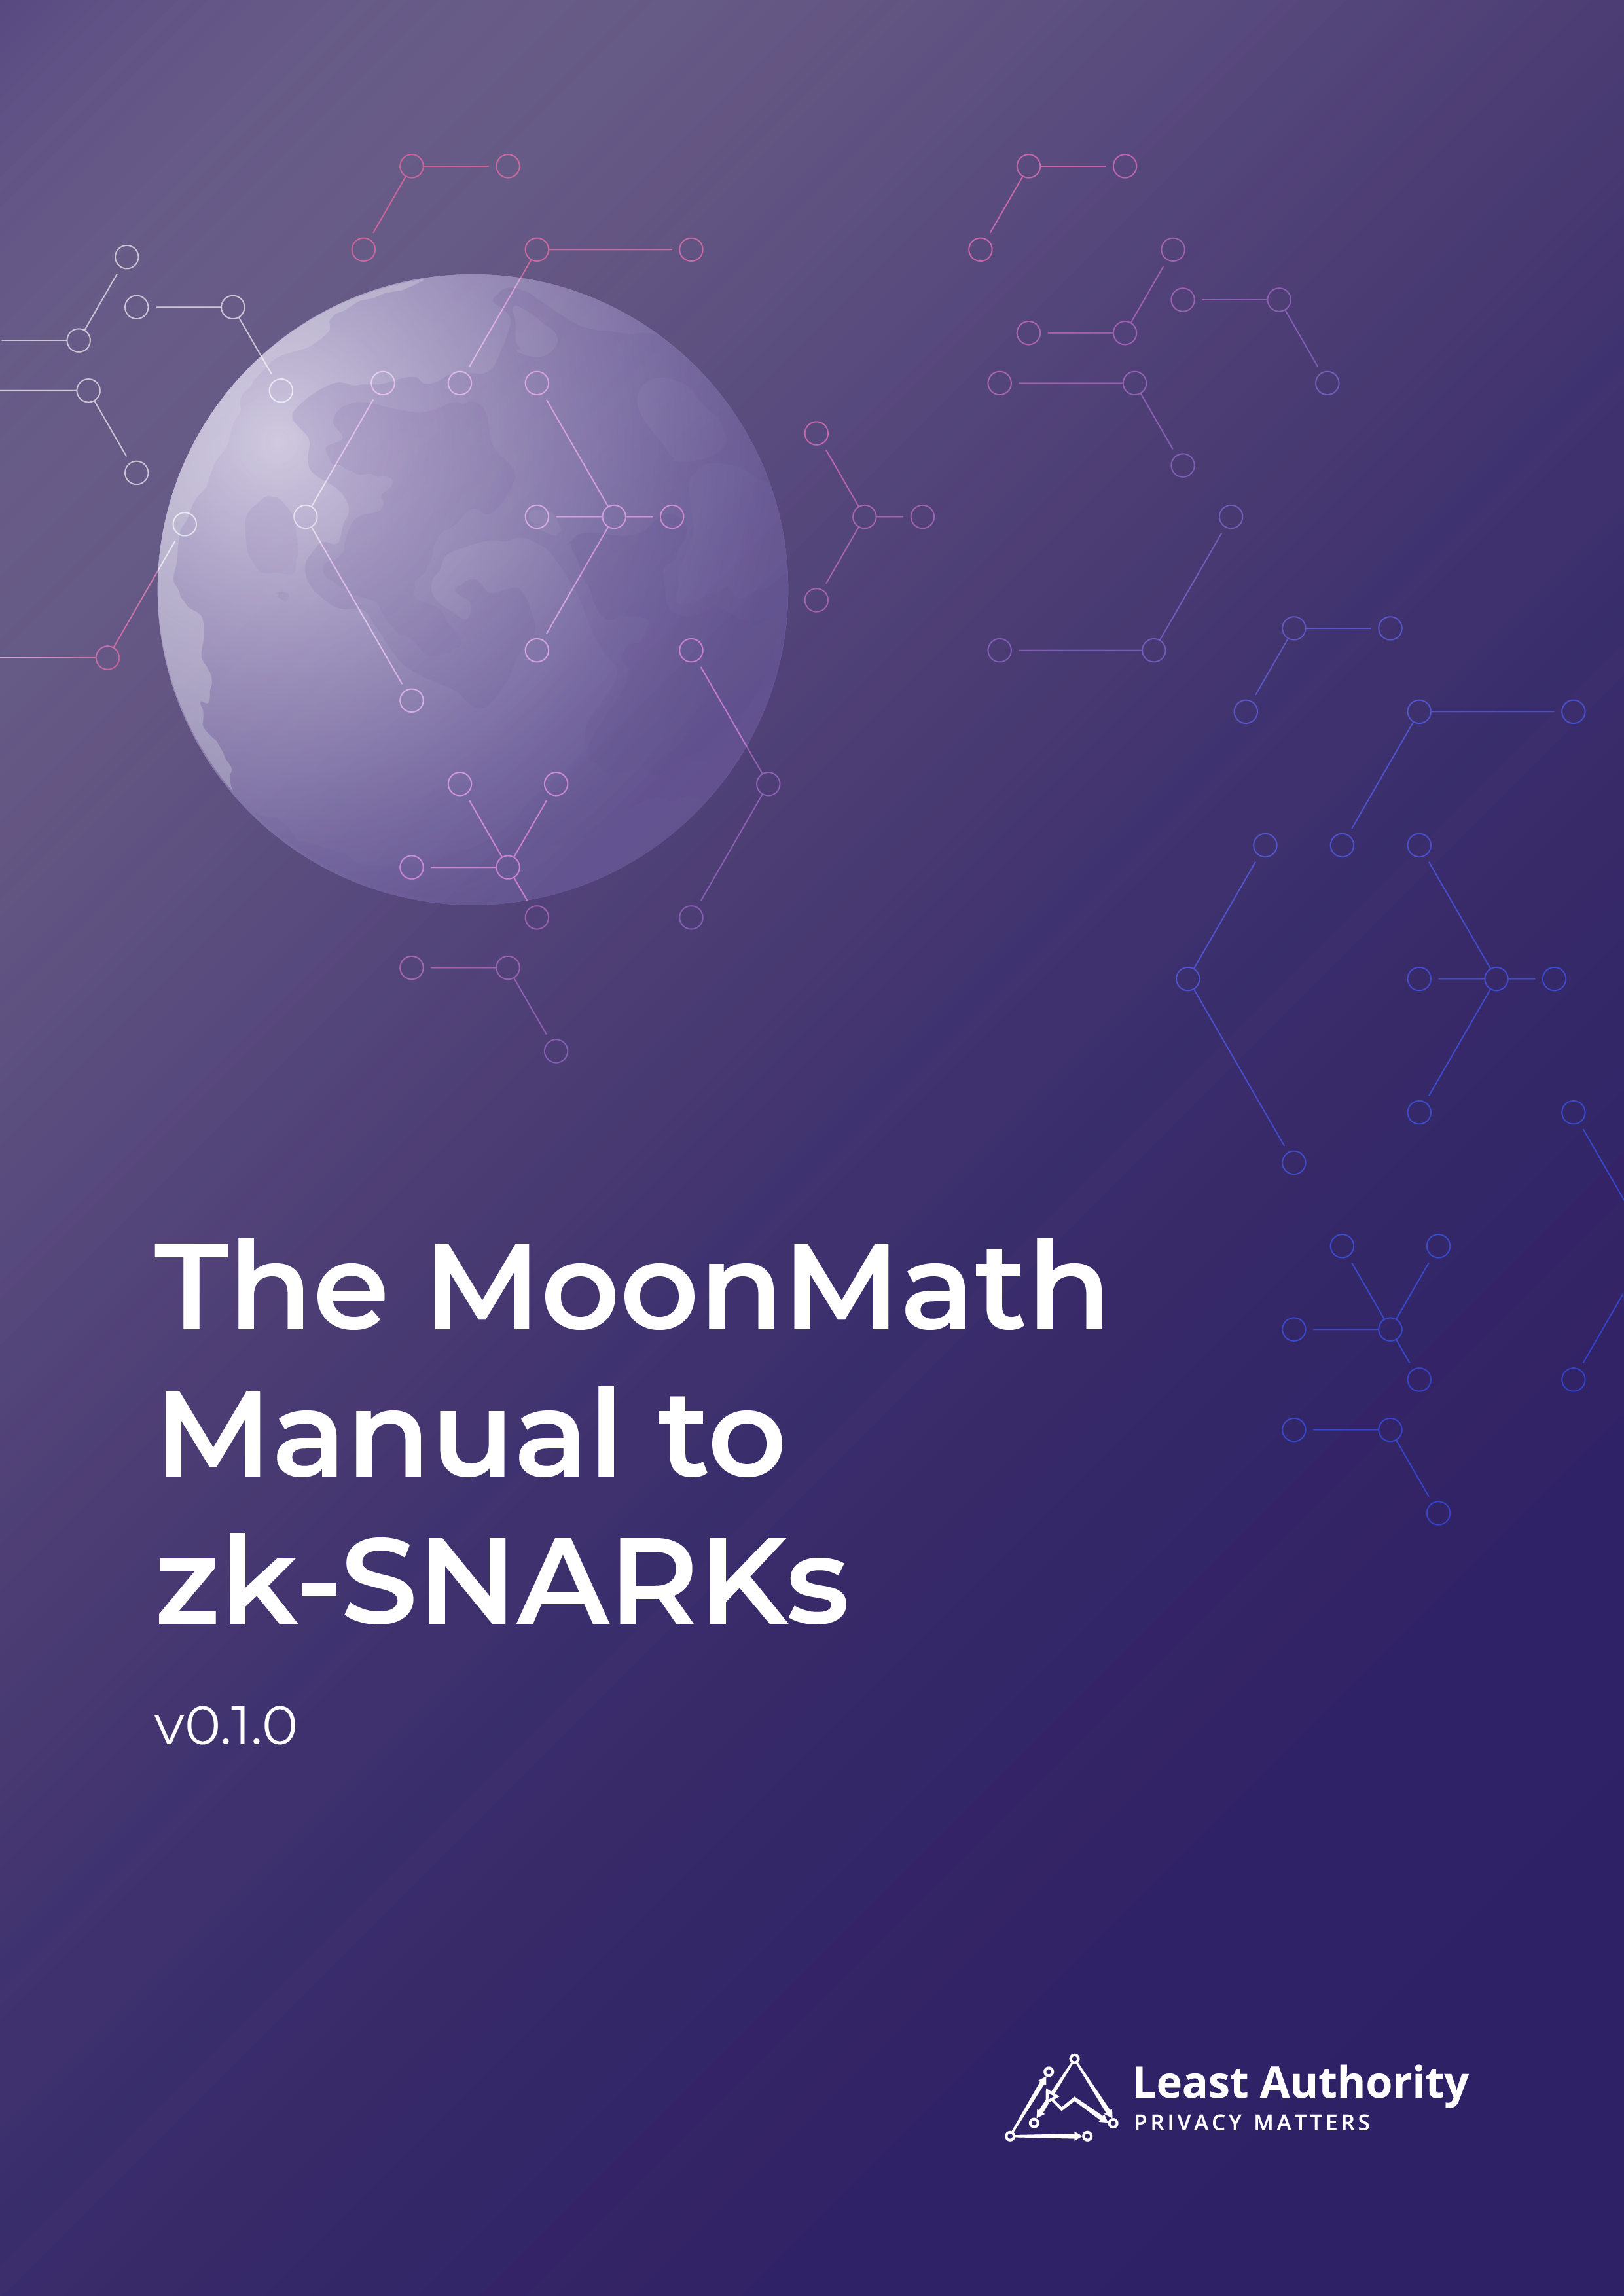
\includepdf{figures/LA_MoonMath_Manual_Cover_Text.png}
 

\begin{center}\Large
Creative Commons Attribution-NonCommercial-NoDerivatives 4.0 International Public License
\end{center}


By exercising the Licensed Rights (defined below), You accept and agree to be bound by the terms and conditions of this Creative Commons Attribution-NonCommercial-NoDerivatives 4.0 International Public License (``Public License''). To the extent this Public License may be interpreted as a contract, You are granted the Licensed Rights in consideration of Your acceptance of these terms and conditions, and the Licensor grants You such rights in consideration of benefits the Licensor receives from making the Licensed Material available under these terms and conditions.

\subsection*{Section 1 – Definitions.}
\begin{itemize}
\item[a.] \textbf{Adapted Material} means material subject to Copyright and Similar Rights that is derived from or based upon the Licensed Material and in which the Licensed Material is translated, altered, arranged, transformed, or otherwise modified in a manner requiring permission under the Copyright and Similar Rights held by the Licensor. For purposes of this Public License, where the Licensed Material is a musical work, performance, or sound recording, Adapted Material is always produced where the Licensed Material is synched in timed relation with a moving image.

\item[b.] \textbf{Copyright and Similar Rights} means copyright and/or similar rights closely related to copyright including, without limitation, performance, broadcast, sound recording, and Sui Generis Database Rights, without regard to how the rights are labeled or categorized. For purposes of this Public License, the rights specified in Section \href{https://creativecommons.org/licenses/by-nc-nd/4.0/legalcode#s2b}{2(b)(1)-(2)} are not Copyright and Similar Rights.

\item[c.] \textbf{Effective Technological Measures} means those measures that, in the absence of proper authority, may not be circumvented under laws fulfilling obligations under Article 11 of the WIPO Copyright Treaty adopted on December 20, 1996, and/or similar international agreements.

\item[d.] \textbf{Exceptions and Limitations} means fair use, fair dealing, and/or any other exception or limitation to Copyright and Similar Rights that applies to Your use of the Licensed Material.

\item[e.] \textbf{Licensed Material} means the artistic or literary work, database, or other material to which the Licensor applied this Public License.

\item[f.] \textbf{Licensed Rights} means the rights granted to You subject to the terms and conditions of this Public License, which are limited to all Copyright and Similar Rights that apply to Your use of the Licensed Material and that the Licensor has authority to license.

\item[g.] \textbf{Licensor} means the individual(s) or entity(ies) granting rights under this Public License.

\item[h.] \textbf{NonCommercial} means not primarily intended for or directed towards commercial advantage or monetary compensation. For purposes of this Public License, the exchange of the Licensed Material for other material subject to Copyright and Similar Rights by digital file-sharing or similar means is NonCommercial provided there is no payment of monetary compensation in connection with the exchange.

\item[i.] \textbf{Share} means to provide material to the public by any means or process that requires permission under the Licensed Rights, such as reproduction, public display, public performance, distribution, dissemination, communication, or importation, and to make material available to the public including in ways that members of the public may access the material from a place and at a time individually chosen by them.

\item[j.] \textbf{Sui Generis Database Rights} means rights other than copyright resulting from Directive 96/9/EC of the European Parliament and of the Council of 11 March 1996 on the legal protection of databases, as amended and/or succeeded, as well as other essentially equivalent rights anywhere in the world.

\item[k.] \textbf{You} means the individual or entity exercising the Licensed Rights under this Public License. Your has a corresponding meaning.
\end{itemize}

\subsection*{Section 2 – Scope.}
\begin{itemize}
\item[a.] \textbf{License grant.}
	\begin{enumerate}
	\item Subject to the terms and conditions of this Public License, the Licensor hereby grants You a worldwide, royalty-free, non-sublicensable, non-exclusive, irrevocable license to exercise the Licensed Rights in the Licensed Material to:
	\begin{enumerate}
		\item[A.] reproduce and Share the Licensed Material, in whole or in part, for NonCommercial purposes only; and
		\item[B.] produce and reproduce, but not Share, Adapted Material for NonCommercial purposes only.
	\end{enumerate}
	\item \underline{Exceptions and Limitations.} For the avoidance of doubt, where Exceptions and Limitations apply to Your use, this Public License does not apply, and You do not need to comply with its terms and conditions.
	\item \underline{Term.} The term of this Public License is specified in Section \href{https://creativecommons.org/licenses/by-nc-nd/4.0/legalcode#s6a}{6(a)}.
	\item \underline{Media and formats; technical modifications allowed.} The Licensor authorizes You to exercise the Licensed Rights in all media and formats whether now known or hereafter created, and to make technical modifications necessary to do so. The Licensor waives and/or agrees not to assert any right or authority to forbid You from making technical modifications necessary to exercise the Licensed Rights, including technical modifications necessary to circumvent Effective Technological Measures. For purposes of this Public License, simply making modifications authorized by this Section \href{https://creativecommons.org/licenses/by-nc-nd/4.0/legalcode#s2a4}{2(a)(4)} never produces Adapted Material.
	\item \underline{Downstream recipients.}
		\begin{enumerate}
		\item[A.] \underline{Offer from the Licensor – Licensed Material.} Every recipient of the Licensed Material automatically receives an offer from the Licensor to exercise the Licensed Rights under the terms and conditions of this Public License.
		\item[B.] \underline{No downstream restrictions.} You may not offer or impose any additional or different terms or conditions on, or apply any Effective Technological Measures to, the Licensed Material if doing so restricts exercise of the Licensed Rights by any recipient of the Licensed Material.
		\end{enumerate}
\item \underline{No endorsement.} Nothing in this Public License constitutes or may be construed as permission to assert or imply that You are, or that Your use of the Licensed Material is, connected with, or sponsored, endorsed, or granted official status by, the Licensor or others designated to receive attribution as provided in Section \href{https://creativecommons.org/licenses/by-nc-nd/4.0/legalcode#s3a1Ai}{3(a)(1)(A)(i)}.
	\end{enumerate}
\item[b.] \textbf{Other rights.}
	\begin{enumerate}
	\item Moral rights, such as the right of integrity, are not licensed under this Public License, nor are publicity, privacy, and/or other similar personality rights; however, to the extent possible, the Licensor waives and/or agrees not to assert any such rights held by the Licensor to the limited extent necessary to allow You to exercise the Licensed Rights, but not otherwise.
	\item Patent and trademark rights are not licensed under this Public License.
	\item To the extent possible, the Licensor waives any right to collect royalties from You for the exercise of the Licensed Rights, whether directly or through a collecting society under any voluntary or waivable statutory or compulsory licensing scheme. In all other cases the Licensor expressly reserves any right to collect such royalties, including when the Licensed Material is used other than for NonCommercial purposes.
	\end{enumerate}
\end{itemize}

\subsection*{Section 3 – License Conditions.}
Your exercise of the Licensed Rights is expressly made subject to the following conditions.
\begin{itemize}
\item[a.] \textbf{Attribution.}
	\begin{enumerate}
	\item If You Share the Licensed Material, You must:
		\begin{enumerate}
		\item[A.] retain the following if it is supplied by the Licensor with the Licensed Material:
			\begin{enumerate}
			\item identification of the creator(s) of the Licensed Material and any others designated to receive attribution, in any reasonable manner requested by the Licensor (including by pseudonym if designated);
			\item a copyright notice;
			\item a notice that refers to this Public License;
			\item a notice that refers to the disclaimer of warranties;
			\item a URI or hyperlink to the Licensed Material to the extent reasonably practicable;
			\end{enumerate}
		\item[B.] indicate if You modified the Licensed Material and retain an indication of any previous modifications; and
		\item[C.] indicate the Licensed Material is licensed under this Public License, and include the text of, or the URI or hyperlink to, this Public License.
		\end{enumerate}
For the avoidance of doubt, You do not have permission under this Public License to Share Adapted Material.
\item You may satisfy the conditions in Section \href{https://creativecommons.org/licenses/by-nc-nd/4.0/legalcode#s3a1A}{3(a)(1)} in any reasonable manner based on the medium, means, and context in which You Share the Licensed Material. For example, it may be reasonable to satisfy the conditions by providing a URI or hyperlink to a resource that includes the required information.
\item If requested by the Licensor, You must remove any of the information required by Section \href{https://creativecommons.org/licenses/by-nc-nd/4.0/legalcode#s3a1A}{3(a)(1)(A)} to the extent reasonably practicable.
	\end{enumerate}
\end{itemize}

\subsection*{Section 4 – Sui Generis Database Rights.}
Where the Licensed Rights include Sui Generis Database Rights that apply to Your use of the Licensed Material:
\begin{itemize}
\item[a.]
for the avoidance of doubt, Section \href{https://creativecommons.org/licenses/by-nc-nd/4.0/legalcode#s2a1}{2(a)(1)} grants You the right to extract, reuse, reproduce, and Share all or a substantial portion of the contents of the database for NonCommercial purposes only and provided You do not Share Adapted Material;
\item[b.] if You include all or a substantial portion of the database contents in a database in which You have Sui Generis Database Rights, then the database in which You have Sui Generis Database Rights (but not its individual contents) is Adapted Material; and
\item[c.] You must comply with the conditions in Section \href{https://creativecommons.org/licenses/by-nc-nd/4.0/legalcode#s3a}{3(a)} if You Share all or a substantial portion of the contents of the database.
\end{itemize}
For the avoidance of doubt, this Section \href{https://creativecommons.org/licenses/by-nc-nd/4.0/legalcode#s4}{4} supplements and does not replace Your obligations under this Public License where the Licensed Rights include other Copyright and Similar Rights.

\subsection*{Section 5 – Disclaimer of Warranties and Limitation of Liability.}
\begin{itemize}
\item[\textbf{a.}] \textbf{Unless otherwise separately undertaken by the Licensor, to the extent possible, the Licensor offers the Licensed Material as-is and as-available, and makes no representations or warranties of any kind concerning the Licensed Material, whether express, implied, statutory, or other. This includes, without limitation, warranties of title, merchantability, fitness for a particular purpose, non-infringement, absence of latent or other defects, accuracy, or the presence or absence of errors, whether or not known or discoverable. Where disclaimers of warranties are not allowed in full or in part, this disclaimer may not apply to You.}
\item[\textbf{b.}] \textbf{To the extent possible, in no event will the Licensor be liable to You on any legal theory (including, without limitation, negligence) or otherwise for any direct, special, indirect, incidental, consequential, punitive, exemplary, or other losses, costs, expenses, or damages arising out of this Public License or use of the Licensed Material, even if the Licensor has been advised of the possibility of such losses, costs, expenses, or damages. Where a limitation of liability is not allowed in full or in part, this limitation may not apply to You.}
\item[c.] The disclaimer of warranties and limitation of liability provided above shall be interpreted in a manner that, to the extent possible, most closely approximates an absolute disclaimer and waiver of all liability.
\end{itemize}

\subsection*{Section 6 – Term and Termination.}
\begin{itemize}
\item[a.] This Public License applies for the term of the Copyright and Similar Rights licensed here. However, if You fail to comply with this Public License, then Your rights under this Public License terminate automatically.
\item[b.] Where Your right to use the Licensed Material has terminated under Section \href{https://creativecommons.org/licenses/by-nc-nd/4.0/legalcode#s6a}{6(a)}, it reinstates:
	\begin{enumerate}
	\item automatically as of the date the violation is cured, provided it is cured within 30 days of Your discovery of the violation; or
	\item upon express reinstatement by the Licensor.
	\end{enumerate}
For the avoidance of doubt, this Section \href{https://creativecommons.org/licenses/by-nc-nd/4.0/legalcode#s6b}{6(b)} does not affect any right the Licensor may have to seek remedies for Your violations of this Public License.
\item[c.] For the avoidance of doubt, the Licensor may also offer the Licensed Material under separate terms or conditions or stop distributing the Licensed Material at any time; however, doing so will not terminate this Public License.
\item[d.] Sections \href{https://creativecommons.org/licenses/by-nc-nd/4.0/legalcode#s1}{1}, \href{https://creativecommons.org/licenses/by-nc-nd/4.0/legalcode#s5}{5}, \href{https://creativecommons.org/licenses/by-nc-nd/4.0/legalcode#s6}{6}, \href{https://creativecommons.org/licenses/by-nc-nd/4.0/legalcode#s7}{7}, and \href{https://creativecommons.org/licenses/by-nc-nd/4.0/legalcode#s8}{8} survive termination of this Public License.
\end{itemize}

\subsection*{Section 7 – Other Terms and Conditions.}
\begin{itemize}
\item[a.] The Licensor shall not be bound by any additional or different terms or conditions communicated by You unless expressly agreed.
\item[b.] Any arrangements, understandings, or agreements regarding the Licensed Material not stated herein are separate from and independent of the terms and conditions of this Public License.
\end{itemize}

\subsection*{Section 8 – Interpretation.}
\begin{itemize}
\item[a.] For the avoidance of doubt, this Public License does not, and shall not be interpreted to, reduce, limit, restrict, or impose conditions on any use of the Licensed Material that could lawfully be made without permission under this Public License.
\item[b.] To the extent possible, if any provision of this Public License is deemed unenforceable, it shall be automatically reformed to the minimum extent necessary to make it enforceable. If the provision cannot be reformed, it shall be severed from this Public License without affecting the enforceability of the remaining terms and conditions.
\item[c.] No term or condition of this Public License will be waived and no failure to comply consented to unless expressly agreed to by the Licensor.
\item[d.] Nothing in this Public License constitutes or may be interpreted as a limitation upon, or waiver of, any privileges and immunities that apply to the Licensor or You, including from the legal processes of any jurisdiction or authority.
\end{itemize}

Creative Commons is not a party to its public licenses. Notwithstanding, Creative Commons may elect to apply one of its public licenses to material it publishes and in those instances will be considered the “Licensor.” The text of the Creative Commons public licenses is dedicated to the public domain under the \href{https://creativecommons.org/publicdomain/zero/1.0/legalcode}{\textsl{CC0 Public Domain Dedication}}. Except for the limited purpose of indicating that material is shared under a Creative Commons public license or as otherwise permitted by the Creative Commons policies published at \href{https://creativecommons.org/policies}{creativecommons.org/policies}, Creative Commons does not authorize the use of the trademark “Creative Commons” or any other trademark or logo of Creative Commons without its prior written consent including, without limitation, in connection with any unauthorized modifications to any of its public licenses or any other arrangements, understandings, or agreements concerning use of licensed material. For the avoidance of doubt, this paragraph does not form part of the public licenses.

Creative Commons may be contacted at \href{creativecommons.org}{creativecommons.org}.

\begin{center}\Large 
Sideletter for Contributions to the MoonMath Manual To zk-SNARKs (the ``\textbf{Sideletter}'')
\end{center}

between Least Authority TFA GmbH, Thaerstraße 28a, 10249 Berlin (hereinafter referred to as ``\textbf{Least Authority}'') and any natural person or legal entity submitting Contributions to the MoonMath Manual (hereinafter referred to as ``\textbf{You}'' or ``\textbf{Your}''). 
\begin{center}\bfseries
Preamble
\end{center}
\begin{itemize}
\item[(A)] Least Authority is the initial creator of the so-called MoonMath Manual To zk-SNARKs (the ``\textbf{Manual}'') which serves as a resource for anyone interested in understanding and unlocking the potential of the so-called ``zk-SNARK'' technology (``\textbf{zk-SNARK}''). The acronym zk-SNARK stands for “Zero-Knowledge Succinct Non-Interactive Argument of Knowledge” and refers to a cryptographic technique where one can prove possession of certain information without revealing the information itself. Most explanations struggle to clarify how and why they work. Resources are scattered across blog posts and Github libraries. This results in a high barrier to entry, thereby slowing the widespread adoption of zk-SNARKs and associated privacy-enhancing technologies. 
\item[(B)] Least Authority wants to change that with the Manual by continuing the Manual as a community-based project to collect useful and practical information on the zk-SNARK. Third-party authors like You shall be able to contribute parts, ideas and practical information to the Manual. 
\item[(C)] The Manual itself is licensed under the Creative Commons Public License, version \textsl{Attri\-bution-NonCommercial-NoDerivatives 4.0 International} (``\textbf{CC BY-NC-ND-4.0}''), which allows usage and distribution as well as modification of the Manual. However, if You modify the Manual or create ``\textbf{Adapted Material}'' of the Manual in the sense of Section 1.a. of the CC BY-NC-ND-4.0, those are not allowed to be distributed by You because Section 3.a.1. subsection 2 of the CC BY-NC-ND-4.0 prohibits the distribution of Adapted Material. 
\item[(D)] If You wish to participate in the Manual, You can submit Adapted Material on the Manual as well as material created independently from the Manual (``\textbf{Independent Creations}'') to Least Authority. If You are interested in adding a major Contribution to the Manual, please contact Least Authority directly under \href{mailto:mmm@leastauthority.com}{mmm@leastauthority.com} and we can discuss if Your contribution can be handled individually with different terms.
\item[(E)] Subject of this Sideletter shall be the licensing of Your Contribution to Least Authority. 
\end{itemize}
Now it is agreed as follows:

\begin{center}
$\S$1\\\bfseries
License on Your Submitted Contribution
\end{center}

\begin{itemize}
\item[(1)] You can contribute any written work, graphic, calculation method, compilation of information, database, or any other work of authorship, including any modifications or additions to the Manual that is created by You by submitting it to Least Authority for the purpose of the inclusion in the Manual, regardless of whether it is an Independent Creation or Adapted Material (each of them a ``\textbf{Contribution}''). ``\textbf{Submission}'' in this sense includes any form of electronic, verbal, or written communication sent to Least Authority under \href{mailto:mmm@leastauthority.com}{mmm@leastauthority.com} or uploaded to https://github.com/LeastAuthority/moonmath-manual. For clarity: Least Authority is not obligated to include Your Contribution in the Manual.

\item[(2)] You hereby grant Least Authority a perpetual, worldwide, non-exclusive, sublicensable, irrevocable and royalty-free right to use, modify, edit, make publicly available and distribute Your Contribution in tangible and intangible form or any other way now known or in the future developed in their original or modified way (within the limits of the prohibition of defacement), as well as to combine it in the original or modified way with or into the Manual (``\textbf{License}''). The License does at least include all rights required to license the Contribution under the CC BY-NC-ND-4.0 and in particular allows Least Authority to use, modify, edit, make publicly available and distribute in tangible and intangible form or any other way now known or in the future developed the Contribution as part of the Manual. Least Authority hereby accepts the grant of the License. 
\item[(3)] If Least Authority decides that Your Contribution or parts thereof shall be included in the Manual, Least Authority will ensure the following: 
	\begin{itemize}
	\item[a)] the Contribution as part of the Manual is licensed under the CC BY-NC-ND-4.0, 
	\item[b)]You will be identified as a Contributor (including by pseudonym if designated) in the Manual. 
	\end{itemize}
The rule § 1 (3) b) only applies if Your name or pseudonym is supplied with the Contribution. 
\item[(4)] In case Least Authority decides that only parts or revisions of Your Contribution will be included in the Manual, Least Authority will inform You within a reasonable period of time and obtain Your consent to license the parts / revisions of Your Contribution corresponding to §1 (2). No consent is needed if only editorial changes are made by Least Authority. In case You decide to submit Your Contribution with no information to contact You, this clause § 1 (4) shall not apply since Least Authority has no possibility to obtain Your consent.      
\item[(5)] In case Least Authority decides that Your Contribution will not be part of the Manual, Least Authority shall use reasonable means to inform you on its decision within a reasonable period of time after Your Submission. The License You granted to Least Authority ends with the decision by Least Authority not to include the Contributions into the Manual. 
\end{itemize}

\begin{center}
$\S$2\\\bfseries
Disclaimer
\end{center}
\begin{itemize}
\item[(1)] Unless otherwise separately undertaken by You, to the extent possible, You offer the Contribution as-is and as-available, and make no representations or warranties of any kind concerning the Contribution, whether express, implied, statutory, or other. This includes, without limitation, warranties of title, merchantability, fitness for a particular purpose, non-infringement, absence of latent or other defects, accuracy, or the presence or absence of errors, whether or not known or discoverable. Where disclaimers of warranties are not allowed in full or in part, this disclaimer may not apply to You.
\item[(2)] To the extent possible, in no event will You be liable to us on any legal theory (including, without limitation, negligence) or otherwise for any direct, special, indirect, incidental, consequential, punitive, exemplary, or other losses, costs, expenses, or damages arising out of this Side Letter or use of the Contribution, even if You have been advised of the possibility of such losses, costs, expenses, or damages. Where a limitation of liability is not allowed in full or in part, this limitation may not apply to You.
\item[(3)] The disclaimer of warranties and limitation of liability provided above shall be interpreted in a manner that, to the extent possible, most closely approximates an absolute disclaimer and waiver of all liability.
\end{itemize}

\begin{center}
$\S$3\\\bfseries
Miscellaneous
\end{center}

\begin{itemize}
\item[(1)] This Sideletter is valid without signature. It is concluded between You and Least Authority at the time of the submission of the Contribution by You to Least Authority. 
\item[(2)] This Sideletter and its interpretation and any non-contractual obligations in connection with it are subject to German substantive law. The UN Convention on Contracts for the International Sale of Goods (CISG) shall not apply.
\item[(3)] English language terms used in this Sideletter describe German legal concepts only and shall not be interpreted by reference to any meaning attributed to them in any jurisdiction other than Germany. Where a German term has been inserted in brackets and/or italics it alone (and not the English term to which it relates) shall be authoritative for the purpose of the interpretation of the relevant term whenever it is used in this Agreement.
\item[(4)] Should one or more provisions of this Sideletter be or become invalid or unenforceable in whole or in part, this shall not affect the validity and enforceability of the remaining provisions of this Sideletter. In place of any Standard Terms of Business (\textsl{Allgemeine Geschäftsbedingungen}) which are invalid or not incorporated in the Sideletter the statutory provisions shall apply (§ 306 (2) of the German Civil Code (BGB)). In all other cases, the parties shall agree a valid provision to replace the invalid or unenforceable provision which reflects as closely as possible the original economic purpose, provided a supplementary interpretation of the Sideletter (\textsl{ergänzende Vertragsauslegung}) does not have precedence or is not possible.
\item[(5)] Amendments and additions to this Sideletter shall be valid only if made in writing. This also applies to any amendment to this written form clause. 
\item[(6)] Any disputes arising out of or in connection with this Sideletter, including disputes on its conclusion, binding effects, amendment and termination, shall be dealt with exclusively by the competent court in Berlin, Germany, if legally possible.
\end{itemize}




%\include{chapters/ops-notes-moonmath}
\tableofcontents

\mainmatter


\chapter{Introduction}
% ATTENTION! THIS IS ALL COPY PASTED FROM SOMEWHERE; SO CAN ONLY BE USED AS GUIDENCE AND NEEDS TO BE REWRITTEN

% Climate Dao whitepaper
\begin{comment}
Zero knowledge proofs are a class of cryptographic protocols in which one can prove
honest computation without revealing the inputs to that computation. A simple high-level
example of a zero-knowledge proof is the ability to prove one is of legal voting age
without revealing the respective age. In a typical zero knowledge proof system, there
are two participants: a prover and a verifier. A prover will present a mathematical proof
of computation to a verifier to prove honest computation. The verifier will then confirm
whether the prover has performed honest computation based on predefined methods.
Zero knowledge proofs are of particular interest to public blockchain activities as the
verifier can be codified in smart contracts as opposed to trusted parties or third-party
intermediaries.

% https://docs.zkproof.org/reference.pdf

Zero-knowledge proofs (ZKPs) are an important privacy-enhancing tool from cryptography. Theyallow proving the veracity of a statement, related to confidential data, without revealing any in-formation beyond the validity of the statement. ZKPs were initially developed by the academiccommunity in the 1980s, and have seen tremendous improvements since then. They are now ofpractical feasibility in multiple domains of interest to the industry, and to a large community ofdevelopers and researchers. ZKPs can have a positive impact in industries, agencies, and for per-sonal use, by allowing privacy-preserving applications where designated private data can be madeuseful to third parties, despite not being disclosed to them. 

ZKP systems involve at least two parties: a prover and a verifier. The goal of the prover is toconvince the verifier that a statement is true, without revealing any additional information. Forexample, suppose the prover holds a birth certificate digitally signed by an authority. In orderto access some service, the prover may have to prove being at least 18 years old, that is, thatthere exists a birth certificate, tied to the identify of the prover and digitally signed by a trustedcertification authority, stating a birthdate consistent with the age claim. A ZKP allows this, withoutthe prover having to reveal the birthdate.
\end{comment}

\section{Target audience}

% copy pasted from https://claritybook.netlify.app/ch00-00-introduction.html
% need adoption to our case
This book is accessible for both beginners and experienced developers alike. Concepts are gradually introduced in a logical and steady pace. Nonetheless, the chapters lend themselves rather well to being read in a different order. More experienced developers might get the most benefit by jumping to the chapters that interest them most. If you like to learn by example, then you should go straight to the chapter on Using Clarinet.

It is assumed that you have a basic understanding of programming and the underlying logical concepts. The first chapter covers the general syntax of Clarity but it does not delve into what programming itself is all about. If this is what you are looking for, then you might have a more difficult time working through this book unless you have an (undiscovered) natural affinity for such topics. Do not let that dissuade you though, find an introductory programming book and press on! The straightforward design of Clarity makes it a great first language to pick up.

\begin{comment}
\section{The Zoo of Zero-Knowledge Proofs}

{First, a list of zero-knowledge proof systems:

\begin{enumerate}
	\item Pinocchio (2013): \href{https://eprint.iacr.org/2013/279.pdf}{{Paper}}
	\begin{itemize}[label={--}]
		\item Notes: trusted setup
	\end{itemize}

	\item BCGTV (2013): \href{https://eprint.iacr.org/2013/507.pdf}{{Paper}}
	\begin{itemize}[label={--}]
		\item Notes: trusted setup, implementation
	\end{itemize}

	\item BCTV (2013): \href{https://eprint.iacr.org/2013/879.pdf}{{Paper}}
	\begin{itemize}[label={--}]
		\item Notes: trusted setup, implementation
	\end{itemize}

	\item Groth16 (2016): 	\href{https://eprint.iacr.org/2016/260.pdf}{Paper}
	\begin{itemize}[label={--}]
		\item Notes: trusted setup
		\item Other resources: \href{https://www.gakonst.com/zksummit2019.pdf}{Talk in 2019 by Georgios Konstantopoulos}
	\end{itemize}

	\item GM17 (207): 	\href{https://eprint.iacr.org/2017/540.pdf}{Paper}
	\begin{itemize}[label={--}]
		\item Notes: trusted setup
		\item Other resources: later \href{https://eprint.iacr.org/2018/187}{Simulation extractability in ROM, 2018}
	\end{itemize}

	\item Bulletproofs (2017): \href{https://eprint.iacr.org/2017/1066.pdf}{Paper}
	\begin{itemize}[label={--}]
		\item Notes: no trusted setup
		\item Other resources: \href{https://eprint.iacr.org/2016/263.pdf}{Polynomial Commitment Scheme on DL, 2016} and \href{https://www.iacr.org/archive/asiacrypt2010/6477178/6477178.pdf}{KZG10, Polynomial Commitment Scheme on Pairings, 2010}
	\end{itemize}

	\item Ligero (2017): \href{https://acmccs.github.io/papers/p2087-amesA.pdf}{Paper}
	\begin{itemize}[label={--}]
		\item Notes: no trusted setup
		\item Other resources: 
	\end{itemize}

	\item Hyrax (2017): \href{https://eprint.iacr.org/2017/1132.pdf}{Paper}
	\begin{itemize}[label={--}]
		\item Notes: no trusted setup
		\item Other resources: 
	\end{itemize}

	\item STARKs (2018): \href{https://eprint.iacr.org/2018/046.pdf}{Paper}
	\begin{itemize}[label={--}]
		\item Notes: no trusted setup 
		\item Other resources: 
	\end{itemize}

	\item Aurora (2018): \href{https://eprint.iacr.org/2018/828.pdf}{Paper}
	\begin{itemize}[label={--}]
		\item Notes: transparent SNARK
		\item Other resources:
	\end{itemize}

	\item Sonic (2019): \href{https://eprint.iacr.org/2019/099.pdf}{Paper}
	\begin{itemize}[label={--}]
		\item Notes: SNORK - SNARK with universal and updateable trusted setup, PCS-based
		\item Other resources: \href{https://www.benthamsgaze.org/2019/02/07/introducing-sonic-a-practical-zk-snark-with-a-nearly-trustless-setup/}{Blog post by Mary Maller from 2019} and \href{https://eprint.iacr.org/2018/280}{work on updateable and universal setup from 2018}
	\end{itemize}

	\item Libra (2019): \href{https://eprint.iacr.org/2019/317}{Paper}
	\begin{itemize}[label={--}]
		\item Notes: trusted setup
		\item Other resources:
	\end{itemize}

	\item Spartan (2019): \href{https://eprint.iacr.org/2019/550.pdf}{Paper}
	\begin{itemize}[label={--}]
		\item Notes: transparent SNARK
		\item Other resources:
	\end{itemize}

	\item PLONK (2019): \href{https://eprint.iacr.org/2019/953.pdf}{Paper}
	\begin{itemize}[label={--}]
		\item Notes: SNORK, PCS-based
		\item Other resources: \href{https://www.plonk.cafe/t/welcome-to-discussion-of-plonk-related-research/24}{Discussion on Plonk systems} and \href{https://github.com/Fluidex/awesome-plonk}{Awesome Plonk list}
	\end{itemize}

	\item Halo (2019): \href{https://eprint.iacr.org/2019/1021}{Paper}
	\begin{itemize}[label={--}]
		\item Notes: no trusted setup, PCS-based, recursive
		\item Other resources: 
	\end{itemize}

	\item Marlin (2019): \href{https://eprint.iacr.org/2019/1047.pdf}{Paper}
	\begin{itemize}[label={--}]
		\item Notes: SNORK, PCS-based
		\item Other resources: \href{https://github.com/arkworks-rs/marlin}{Rust Github}
	\end{itemize}

	\item Fractal (2019): \href{https://eprint.iacr.org/2019/1076.pdf}{Paper}
	\begin{itemize}[label={--}]
		\item Notes: Recursive, transparent SNARK
		\item Other resources: 
	\end{itemize}

	\item SuperSonic (2019): \href{https://eprint.iacr.org/2019/1229.pdf}{Paper}
	\begin{itemize}[label={--}]
		\item Notes: transparent SNARK, PCS-based
		\item Other resources: \href{https://eprint.iacr.org/2021/358}{Attack on DARK compiler in 2021}
	\end{itemize}

	\item Redshift (2019): \href{https://eprint.iacr.org/2019/1400}{Paper}
	\begin{itemize}[label={--}]
		\item Notes: SNORK, PCS-based
		\item Other resources: 
	\end{itemize}



\end{enumerate}

\textbf{Other resources on the zoo: } \href{https://github.com/matter-labs/awesome-zero-knowledge-proofs}{Awesome ZKP list on Github}, \href{https://zkp.science/}{ZKP community} with the \href{https://docs.zkproof.org/reference.pdf}{reference document}

}

\paragraph{To Do List}
\begin{itemize}
	\item Make table for prover time, verifier time, and proof size
	\item Think of categories - \textit{Achieved Goals}: Trusted setup or not, Post-quantum or not, \dots
	\item Think of categories - \textit{Mathematical background}: Polynomial commitment scheme, \dots
	\item \dots while we discuss the points above, we should also discuss a common notation/language for all these things. (E.g. transparent SNARK/no trusted setup/STARK)
\end{itemize}

\paragraph{Points to cover while writing}
\begin{itemize}
	\item Make a historical overview over the "discovery" of the different ZKP systems
	\item Make reader understand what paper is build on what result etc. - the tree of publications!
	\item Make reader understand the different terminology, e.g. SNARK/SNORK/STARK, PCS, R1CS, updateable, universal, $\dots$
	\item Make reader understand the mathematical assumptions - and what this means for the zoo.
	\item Where will the development/evolution go? What are bottlenecks?
\end{itemize}

\vspace*{1em}
{\footnotesize
\hspace*{-1em}\textbf{Other topics I fell into while compiling this list}
\begin{itemize}
	\item Vector commitments: \url{https://eprint.iacr.org/2020/527.pdf}
	\item Snarkl: \url{http://ace.cs.ohio.edu/~gstewart/papers/snaarkl.pdf}
	\item Virgo?: \url{https://people.eecs.berkeley.edu/~kubitron/courses/cs262a-F19/projects/reports/project5_report_ver2.pdf}
\end{itemize} 
}

\end{comment}



\chapter{Preliminaries}

\section{Preface and Acknowledgements}
This book began as a set of lecture and notes accompanying the zk-Summit 0x and 0xx .... It arose from the desire to collect the scattered information of snarks [] and present them to an audience that does not have a strong backgroud in cryptography []

\section{Purpose of the book}
The first version of this book is written by security auditors at Least Authority where we audited quite a few snark based systems. Its included "what we have learned" destilate of the time we spend on various audits.  


We intend to let illus-
trative examples drive the discussion and present the key concepts of pairing
computation with as little machinery as possible. For those that are fresh to
pairing-based cryptography, it is our hope that this chapter might be particu-
larly useful as a first read and prelude to more complete or advanced expositions
(e.g. the related chapters in [Gal12]).

On the other hand, we also hope our beginner-friendly intentions do not leave
any sophisticated readers dissatisfied by a lack of formality or generality, so in
cases where our discussion does sacrifice completeness, we will at least endeavour
to point to where a more thorough exposition can be found.

One advantage of writing a survey on pairing computation in 2012 is that,
after more than a decade of intense and fast-paced research by mathematicians
and cryptographers around the globe, the field is now racing towards full matu-
rity. Therefore, an understanding of this text will equip the reader with most
of what they need to know in order to tackle any of the vast literature in this
remarkable field, at least for a while yet.

Since we are aiming the discussion at
active readers, we have matched every example with a corresponding snippet of
(hyperlinked) Magma [BCP97] code 1 , where we take inspiration from the helpful
Magma pairing tutorial by Dominguez Perez et al. [DKS09].

Early in the book we will develop examples that we then later extend with most of the things we learn in each chapter. This way we incrementally build a few real world snarks but over full fledged cryptographic systems that are nevertheless simple enough to be computed by pen and paper to illustrate all steps in great detail.

\begin{comment}

\section{How to read this book}

Books and papers to read: XXXXXXXXXXX

Software to try: XXXXXXXXXXXXXXXXXXX

Correctly prescribing the best reading route for a beginner naturally requires individual diagnosis that depends on their prior knowledge and technical preparation.

\section{Cryptological Systems}
The science of information security is referred to as \textit{cryptology}. In the broadest sense, it deals with encryption and decryption processes, with digital signatures, identification protocols, cryptographic hash functions, secrets sharing, electronic voting procedures and electronic money. EXPAND

\section{SNARKS}



\section{complexity theory}
Before we deal with the mathematics behind zero knowledge proof systems, we must first clarify what is meant by the runtime of an algorithm or the time complexity of an entire mathematical problem. This is particularly important for us when we analyze the various snark systems...

For the reader who is interested in complexity theory, we recommend, or example 
%\cite{BE} 
or 
%\cite{AB}
, as well as the references contained therein.

\subsection{Runtime complexity}
The runtime complexity of an algorithm describes, roughly speaking, the amount of elementary computation steps that this algorithm requires in order to solve a problem, depending on the size of the input data.

Of course, the exact amount of arithmetic operations required depends on many factors such as the implementation, the operating system used, the CPU and many more. However, such accuracy is seldom required and is mostly meaningful to consider only the asymptotic computational effort.

In computer science, the runtime of an algorithm is therefore not specified in individual calculation steps, but instead looks for an upper limit which approximates the runtime as soon as the input quantity becomes very large. This can be done using the so-called \textit{Landau notation} (also called big -$\mathcal{O}$-notation) A precise definition
would, however, go beyond the scope of this work and we therefore refer the reader to 
%\cite{AB}
.

For us, only a rough understanding of transit times is important in order to be able to talk about the security of crypographic systems. For example, $\mathcal{O}(n)$ means that the running time of the algorithm to be considered is linearly dependent on the size of the input set $n$, $\mathcal{O}(n^k)$ means that the running time is polynomial and $\mathcal{O}(2^n) $ stands for an exponential running time (%\cite{JB} 
chapter 2.4).


An algorithm which has a running time that is greater than a polynomial is often simply referred to as \textit{slow}.

A generalization of the runtime complexity of an algorithm is the so-called \textit{time complexity of a mathematical problem}, which is defined as the runtime of the fastest possible algorithm that can still solve this problem (
%\cite{AB} 
chapter 3.1).

Since the time complexity of a mathematical problem is concerned with the runtime analysis of all possible (and thus possibly still undiscovered) algorithms, this is often a very difficult and deep-seated question .

For us, the time complexity of the so-called discrete logarithm problem will be important. This is a problem for which we only know slow algorithms on classical computers at the moment, but for which at the same time we cannot rule out that faster algorithms also exist.
 

STUFF ON CRYPTOGRAPHIC HASH FUNCTIOND

\end{comment}


\section{Software Used in This Book}

\subsection{Sagemath}
\label{sagemath_setup}
It order to provide an interactive learning experience, and to allow getting hands-on with the concepts described in this book, we give examples for how to program them in the Sage programming language. Sage is a dialect of the learning-friendly programming language Python, which was extended and optimized for computing with, in and over algebraic objects. Therefore, we recommend installing Sage before diving into the following chapters.

The installation steps for various system configurations are described on the sage websit \footnote{\url{https://doc.sagemath.org/html/en/installation/index.html}}. Note however that we use Sage version 9, so if you are using Linux and your package manager only contains version 8, you may need to choose a different installation path, such as using prebuilt binaries.

We recommend the interested reader, who is not familiar with sagemath to read on the many tutorial before starting this book. For example 
%https://doc.sagemath.org/pdf/en/tutorial/SageTutorial.pdf

% Note: Logging Input and Output
% You can use this command to log all input you type, all output, and even play back that input in a future session (by simply reloadingthe log file).



\chapter{Arithmetics}\label{chap:arithmetic}\label{chap:arithmetics}

\section{Introduction}

The goal of this chapter is to bring a reader with only basic school-level algebra up to speed in arithmetic. We start with a brief recapitulation of basic integer arithmetics, discussing long division, the greatest common divisor and \concept{Euclidean division}. After that, we introduce modular arithmetic as \hilight{the most important} skill to compute our pen-and-paper examples. We then introduce polynomials, compute their analogs to integer arithmetics and introduce the important concept of \concept{Lagrange interpolation}.

\section{Integer arithmetic}
\label{integer_arithmetic}
In a sense, integer arithmetic is at the heart of large parts of modern cryptography. Fortunately, most readers will probably remember integer arithmetic from school. It is, however, important that you can confidently apply those concepts to understand and execute computations in the many pen-and-paper examples that form an integral part of the MoonMath Manual. We will therefore recapitulate basic arithmetic concepts to refresh your memory and fill any knowledge gaps.

Even though the terms and concepts in this chapter might not appear in the literature on zero-knowledge proofs directly, understanding them is necessary to follow subsequent chapters and beyond: terms like \term{groups} or \term{fields} also crop up very frequently in academic papers on zero-knowledge cryptography.

Many of the ideas presented in this chapter are taught in basic mathematical education in most schools around the globe. Much of the ideas presented in this section can be found in \cite{wu-1}. An approach more oriented towards computer science can be found in \cite{mignotte-1992}.

\subsection{Integers, natural numbers and rational numbers}

Integers are also known as \term{whole numbers}, that is, numbers that can be written without fractional parts. Examples of numbers that are \hilight{not} integers are $\frac{2}{3}$, $1.2$ and $-1280.006$.\footnote{Whole numbers, along with their basic laws of operations, are introduced for example in chapters 1 – 6 of \cite{wu-1}.}

Throughout this book, we use the symbol $\mathbb{Z}$ as a shorthand for the set of all \term{integers}:

\begin{equation}
\label{integer_symbol}
\Z := \{\ldots, -3,-2,-1,0,1,2,3,\ldots\}
\end{equation}

If $a\in \Z$ is an integer, then we write $|a|$ for the \term{absolute value} of $a$, that is, the the non-negative value of $a$ without regard to its sign:

\begin{equation}
|4|= 4
\end{equation}
\begin{equation}
|-4|= 4
\end{equation}

We use the symbol $\N$ for the set of all positive integers, usually called the set of \term{natural numbers}. Furthermore, we use $\NN$ for the set of all non-negative integers. This means that $\mathbb{N}$ does not contain the number $0$, while $\NN$ does:
\begin{align*}
\label{natural_symbol}
\N := \{1,2,3,\ldots\} & & \NN := \{0,1,2,3,\ldots\}
\end{align*}

In addition, we use the symbol $\Q$ for the set of all \term{rational numbers}, which can be represented as the set of all fractions $\frac{n}{m}$, where $n\in \Z$ is an integer and $m\in \N$ is a natural number, such that there is no other fraction $\frac{n'}{m'}$ and natural number $k\in \N$ with $k\neq 1$ and the following equation:\footnote{A more in-depth introduction to rational numbers, their representation as well as their arithmetic operations can be found in part 2. of \cite{wu-1} and in \chaptname{} 1, \secname{} 2 of \cite{mignotte-1992}.}
\begin{equation}
\frac{n}{m} = \frac{k\cdot n'}{k\cdot m'}
\end{equation}

The sets $\N$, $\Z$ and $\Q$ have a notion of addition and multiplication defined on them. Most of us are probably able to do many integer computations in our head, but this gets more and more difficult as these increase in complexity.  We will frequently use the  SageMath system (\ref{sagemath_setup}) for more complicated computations (we define rings and fields later in this book):
\begin{sagecommandline}
sage: ZZ #  Sage notation for the set of integers
sage: NN # Sage notation for the set of natural numbers
sage: QQ # Sage notation for the set of rational numbers
sage: ZZ(5) # Get an element from the set of integers
sage: ZZ(5) + ZZ(3)
sage: ZZ(5) * NN(3)
sage: ZZ.random_element(10**6)
\end{sagecommandline}

A set of numbers of particular interest to us is the set of \term{prime numbers}. A prime number is a natural number $ p \in \N $ with $ p \geq 2 $ that is only divisible by itself and by $1$. All prime numbers apart from the number $ 2 $ are called \term{odd} prime numbers. We use $ \Prim $ for the set of all prime numbers and $ \Prim _{\geq 3} $ for the set of all odd prime numbers.\footnote{As prime numbers are of central importance to our topic, the interested reader might benefit from consulting the wide range of books available on the topic of number theory. An introduction is given for example in  \chaptname{} 1 and 2 of \cite{hardy-2008}. An elementary school level introduction can be found in  \chaptname{} 33 of \cite{wu-1}. Chapter 34 of \cite{wu-1} gives an introduction to the fundamental theorem of arithmetic \eqref{def:fundamental_theorem_arithmetic}. \cite{fine-2016} could be of particular interest to more advanced readers.}

The set of prime numbers $\Prim$ is an infinite set, and it can be ordered according to size. This means that, for any prime number $p\in\Prim$, one can always find another prime number $p'\in\Prim$ with $p<p'$. As a result, there is no largest prime number. Since prime numbers can be ordered by size, we can write them as follows:
\begin{equation}
\label{eq: primenumber_sequence}
2, 3, 5, 7, 11, 13, 17, 19, 23, 29, 31, 37, 41, 43, 47, 53, 59, 61, 67, \ldots
\end{equation}
As the \term{fundamental theorem of arithmetic} tells us, prime numbers are, in a certain sense, the basic building blocks from which all other natural numbers are composed: every natural number can be derived by multiplying prime numbers with each other. To see that, let $ n \in \N $ be any natural number with $n>1$. Then there are always prime numbers $ p_1, p_2, \ldots, p_k \in \Prim $, such that the following equation holds:
\begin{equation}
\label{def:fundamental_theorem_arithmetic}
n = p_1 \cdot p_2 \cdot \ldots \cdot p_k \;
\end{equation}
This representation is unique for each natural number (except for the order of the \term{factors} $ p_1, p_2, \ldots, p_k$) and is called the \term{prime factorization} of $n$.

\begin{example}[Prime Factorization]\label{ex-prime-factorization} To see what we mean by the prime factorization of a number, let's look at the number $504\in\N$. To get its prime factors, we can successively divide it by all prime numbers in ascending order starting with $2$:
\begin{equation*}
504 = 2\cdot 2\cdot 2\cdot 3\cdot 3\cdot 7
\end{equation*}
We can double check our findings invoking  Sage, which provides an algorithm for factoring natural numbers:
\begin{sagecommandline}
sage: n = NN(504)
sage: factor(n)
\end{sagecommandline}
\end{example}

The computation from the previous example reveals an important observation: computing the factorization of an integer is computationally expensive, because we have to divide repeatedly by all prime numbers smaller than the number itself until all factors are prime numbers themselves. From this, an important question arises: how fast can we compute the prime factorization of a natural number? This question is the famous \hilight{integer factorization problem} and, as far as we know, there is currently no known method that can factor integers much faster than the naive approach of just dividing the given number by all prime numbers in ascending order.

On the other hand, computing the product of a given set of prime numbers is fast: you just multiply all factors. This simple observation implies that the two processes, ``prime number multiplication'' on the one side and its inverse process ``natural number factorization'' have very different computational costs. The factorization problem is therefore an example of a so-called \term{one-way function}: an invertible function that is easy to compute in one direction, but hard to compute in the other direction 
%(see Wikipedia for a description of \href{https://en.wikipedia.org/wiki/Time_complexity}{time complexity} and \href{https://en.wikipedia.org/wiki/Time_complexity#Polynomial_time}{polynomial time})
. 
\footnote{It should be noted that what is ``easy'' and ``hard'' to compute depends on the computational power available to us. Currently available computers cannot easily compute the prime factorization of natural numbers (in formal terms, the cannot compute it in polynomial time). However, the American mathematician Peter W. Shor developed an algorithm in \citeyear{shor94} which can calculate the prime factorization of a natural number in polynomial time on a quantum computer. The consequence of this is that cryptosystems, which are based on the prime factor problem being computationally hard on currently available computers, become unsafe as soon as practically usable quantum computers become available.}


\begin{exercise}
What is the absolute value of the integers $-123$, $27$ and $0$?
\end{exercise}
\begin{exercise}
Compute the factorization of $30030$ and double check your results using  Sage.
\end{exercise}
\begin{exercise}
Consider the following equation:
\begin{equation*}4\cdot x + 21 = 5\end{equation*}
Compute the set of all solutions for $x$ under the following alternative assumptions:
\begin{enumerate}
\item The equation is defined over the set of natural numbers.
\item The equation is defined over the set of integers.
\end{enumerate}
\end{exercise}
\begin{exercise}
Consider the following equation:
\begin{equation*} 2 x^3 - x^2 - 2 x = - 1.\end{equation*}
Compute the set of all solutions $x$ under the following assumptions:
\begin{enumerate}
\item The equation is defined over the set ofnatural numbers.
\item The equation is defined over the set of integers.
\item The equation is defined over the set of rational numbers.
\end{enumerate}
\end{exercise}

\subsection{\concept{Euclidean division}}
\label{Euclidean_division}
As we know from high school mathematics, integers can be added, subtracted and multiplied, and the result of these operations is guaranteed to always be an integer as well.
On the contrary, division (in the commonly understood sense) is not defined for integers, as, for example, $7$ divided by $3$ will not result in an integer. However, it is always possible to divide any two integers if we consider \term{division with a remainder}. For example, $7$ divided by $3$ is equal to $2$ with a remainder of $1$, since $7 = 2\cdot 3 + 1$.

This section introduces division with a remainder for integers, usually called \term{\concept{Euclidean division}}. It is an essential technique underlying many concepts in this book.\footnote{\concept{Euclidean division} is introduced in \chaptname{} 1, \secname{} 5 of \cite{mignotte-1992} and in \chaptname{} 1, \secname{} 1.3 of \cite{cohen-2010}.} The precise definition is as follows:

Let $ a \in \Z $ and $ b \in \Z $ be two integers with $b\neq 0$. Then there is always another integer $ m \in \Z $ and a natural number $ r \in \N $, with $ 0 \leq r <|b| $ such that the following holds:
\begin{equation}
\label{eq_euclidean_division}
a = m \cdot b + r
\end{equation}
This decomposition of $a$ given $b$ is called \term{\concept{Euclidean division}}, where $ a $ is called the \term{dividend}, $ b $ is called the \term{divisor}, $m$ is called the \term{quotient} and $r$ is called the \term{remainder}. It can be shown that both the quotient and the remainder always exist and are unique, as long as the divisor is different from $0$.
\begin{notation}
\label{eq_euclidean_division_notation}
Suppose that the numbers $a$, $b$, $m$ and $r$ satisfy equation (\ref{eq_euclidean_division}). We can then use the following notation for the quotient and the remainder of the \concept{Euclidean division} as follows:
\begin{equation}
\label{def_integer_division_and_modulus}
\begin{array}{lcr}
\Zdiv{a}{b}: = m, & & \Zmod{a}{b}: = r
\end{array}
\end{equation}

We also say that an integer $ a $ is \term{divisible} by another integer $ b $ if $ \Zmod{a}{b} = 0 $ holds. In this case, we write $ b | a $, and call the integer $\Zdiv{a}{b}$ the \term{cofactor}\label{def:cofactor} of $b$ in $a$.
\end{notation}
So, in a nutshell, \concept{Euclidean division} is the process of dividing one integer by another in a way that produces a quotient and a non-negative remainder, the latter of which is smaller than the absolute value of the divisor.

\begin{example}
\label{example:euclidean_division_1}
 Because $ -17 = -5 \cdot 4 + 3 $  is the \concept{Euclidean division} of $-17$ by $4$, applying \concept{Euclidean division} and the notation defined in \ref{def_integer_division_and_modulus} to the dividend $-17$ and the divisor $4$, we get the following:
\begin{equation}
\begin{array}{lcr}
\Zdiv{-17}{4} = - 5, & & \Zmod{-17}{4} = 3
\end{array}
\end{equation}
The remainder, by definition, is a non-negative number. In this case, $4$ does not divide $-17$, as the remainder is not zero. The truth value of the expression $4 | -17 $ therefore is \textsc{false}. On the other hand, the truth value of $4 | 12$ is \bool{true}, since $4$ divides $12$, as $ \Zmod{12}{4} = 0 $. If we use  Sage to do the computation for us, we get the following:
\begin{sagecommandline}
sage: ZZ(-17) // ZZ(4) # Integer quotient
sage: ZZ(-17) % ZZ(4) # remainder
sage: ZZ(4).divides(ZZ(-17)) # self divides other
sage: ZZ(4).divides(ZZ(12))
\end{sagecommandline}
\end{example}
\begin{remark} In \ref{def_integer_division_and_modulus}, we defined the notation of  \hilight{$\Zdiv{a}{b}$} and \hilight{$\Zmod{a}{b}$} in terms of \concept{Euclidean division}. It should be noted, however, that many programing languages (like Python and  Sage) implement both the operator $(/)$ amd the operator $(\%)$ differently. Programers should be aware of this, as the discrepancy between the mathematical notation and the implementation in programing languages might become the source of subtle bugs in implementations of cryptographic primitives.

To give an example, consider the the dividend $-17$ and the divisor $-4$. Note that, in contrast to the previous \examplename{} \ref{example:euclidean_division_1}, we now have a negative divisor. According to our definition we have the following:
\begin{equation}\label{euclidean-negative}
\begin{array}{lcr}
\Zdiv{-17}{-4} = 5, & & \Zmod{-17}{-4} = 3
\end{array}
\end{equation}
$ -17 = 5 \cdot (-4) + 3 $  is the \concept{Euclidean division} of $-17$ by $-4$ (the remainder is, by definition, a non-negative number). However, using the operators $(/)$ and $(\%)$ in  Sage, we get a different result: 

\begin{sagecommandline}
sage: ZZ(-17) // ZZ(-4) # Integer quotient
sage: ZZ(-17) % ZZ(-4) # remainder
sage: ZZ(-17).quo_rem(ZZ(-4)) # not Euclidean Division
\end{sagecommandline}
\end{remark}

Methods to compute \concept{Euclidean division} for integers are called \term{integer division algorithms}. Probably the best known algorithm is the so-called \term{long division}, which most of us might have learned in school. An extensive elementary school introduction to long division can be found in \chaptname{} 7 of \cite{wu-1}.

In a nutshell, the long division algorithm loops through the digits of the dividend from the left to right, subtracting the largest possible multiple of the divisor (at the digit level) at each stage. The multiples then become the digits of the quotient, and the remainder is the first digit of the dividend.

As long division is the standard method used for pen-and-paper division of multi-digit numbers expressed in decimal notation, we use it throughout this book when we do simple pen-and-paper computations, so readers should become familiar with it. However, instead of defining the algorithm formally, we  provide some examples instead, as this will hopefully make the process more clear.

\begin{example}[Integer Long Division] To give an example of integer long division algorithm, let's divide the integer $a=143785$ by the number $b=17$. Our goal is therefore to find solutions to equation \ref{eq_euclidean_division}, that is, we need to find the quotient $m\in\Z$ and the remainder $r \in \N$ such that $143785 = m\cdot 17 + r$. Using a notation that is mostly used in English-speaking countries, we compute as follows:\smecomb{SB: I think a more detailed explanation is needed for those unfamiliar with this notation/algorithm. MIRCO: I think we have to make a cut somewhere. Explaining third grade integer division is ot of scope and a requirement to read the book}{Add explanation}
\begin{equation}
\intlongdivision{143785}{17}
\end{equation}
We calculated $m=8457$ and $r=16$, and, indeed, the equation $143785 = 8457\cdot 17 + 16$ holds.  We can double check this invoking  Sage:
\begin{sagecommandline}
sage: ZZ(143785).quo_rem(ZZ(17))
sage: ZZ(143785) == ZZ(8457)*ZZ(17) + ZZ(16) # check
\end{sagecommandline}

\end{example}
\begin{exercise}[Integer Long Division]
Find an $m\in\Z$ and an $r\in\N$ with $0\leq r< |b|$ such that $a= m\cdot b +r$ holds for the following pairs:
\begin{itemize}\compactlist{}
 \item $(a,b) = (27,5)$ 
 \item $(a,b)=(27,-5)$
 \item $(a,b)=(127,0)$
 \item $(a,b)= (-1687, 11)$
 \item $(a,b)= (0, 7)$
 \end{itemize}
 In which cases are your solutions unique?
\end{exercise}
\begin{exercise}[Long Division Algorithm]
Using the programming language of your choice, write an algorithm that computes integer long division and handles all edge cases properly.
\end{exercise}
\begin{exercise}[Binary Representation]
Write an algorithm that computes the binary representation \ref{def:binary_representation_integer} of any non-negative integer.
\end{exercise}

\subsection{The Extended Euclidean Algorithm}
\label{sec:gcd}
One of the most critical parts of this book is the modular arithmetic, defined in section \ref{modular_arithmetic}, and its application in the computations of \term{prime fields}, defined in section \ref{prime_fields}. To be able to do computations in modular arithmetic, we have to get familiar with the so-called \term{Extended Euclidean Algorithm}, used to calculate the \term{greatest common divisor} (GCD) of integers.\footnote{A more in-depth introduction to the content of this section can be found in \chaptname{} 1, \secname{} 1.3 of \cite{cohen-2010} and in \chaptname{} 1, \secname{} 8 of \cite{mignotte-1992}.}

The {greatest common divisor} of two non-zero integers $a$ and $b$ is defined as the largest non-zero natural number $d$ such that $d$ divides both $a$ and $b$, that is, $d|a$ as well as $d|b$ are true. We use the notation $ gcd (a, b):=d $ for this number. Since the natural number $1$ divides any other integer, $1$ is always a common divisor of any two non-zero integers, but it is not necessarily the greatest.

A common method for computing the greatest common divisor is the so-called Euclidean Algorithm. However, since we don't need that algorithm in this book, we will introduce the Extended Euclidean Algorithm, which is a method for calculating the greatest common divisor of two natural numbers $ a $ and $ b \in \N $, as well as two additional integers $ s, t \in \Z $, such that the following equation holds:
\begin{equation}
\label{eq: erw_Eukl_algo}
gcd (a, b) = s \cdot a + t \cdot b
\end{equation}

The pseudocode in algorithm \ref{alg_ext_euclid_alg} shows in detail how to calculate the greatest common divisor and the numbers $s$ and $t$ with the Extended Euclidean Algorithm:

\begin{algorithm}\caption{Extended Euclidean Algorithm}
\label{alg_ext_euclid_alg}
\begin{algorithmic}[0]
\Require $a,b \in \N$ with $a\geq b$
\Procedure{Ext-Euclid}{$a,b$}
\State $r_0\gets a$ and $r_1\gets b$
\State $s_0\gets 1$ and $s_1\gets 0$
\State $t_0\gets 0$ and $t_1\gets 1$
\State $k\gets 2$
\While{$ r_{k-1} \neq 0 $}
\State $ q_k\gets \Zdiv{r_{k-2}}{r_{k-1}} $
\State $ r_{k}\gets \Zmod{r_{k-2}}{r_{k-1}} $
\State $ s_{k}\gets s_{k-2} -q_k \cdot s_{k-1} $
\State $ t_{k}\gets t_{k-2} -q_k \cdot t_{k-1} $
\State $ k \gets k + 1 $
\EndWhile
\State \textbf{return} $gcd(a,b)\gets r_{k-2}$, $s\gets s_{k-2}$ and $ t \gets t_{k-2} $
\EndProcedure
\Ensure $ gcd (a, b) = s \cdot a + t \cdot b $
\end{algorithmic}
\end{algorithm}
The algorithm is simple enough to be used effectively in pen-and-paper examples. It is commonly written as a table where the rows represent the while-loop and the columns represent the values of the the array $r$, $s$ and $t$ with index $k$. The following example provides a simple execution.
\begin{example}
\label{example:extended_Euclidean_division_1}
To illustrate algorithm \ref{alg_ext_euclid_alg}, we apply it to the numbers $a=12$ and $b=5$. Since $12,5\in \N$ and $12\geq 5$, all requirements are met, and we compute as follows:
\begin{center}
  \begin{tabular}{c | c c l}
    k & $ r_k $ & $ s_k $ & $ t_k $ \\\hline
    0 & 12 & 1 & 0 \\
    1 & 5 & 0 & 1 \\
    2 & 2 & 1 & -2 \\
    3 & 1 & -2 & 5 \\
    4 & 0 &  &  \\
    5 & $\cdot$ & &\\
  \end{tabular}
  \end{center}

  
  \begin{comment}
  \begin{tabularx}{1.02\textwidth}{c| r  r  r  r@{}c@{\hspace{0.5cm}}>{\small}X>{\small}X>{\small}X>{\small}X@{}}
    k & $ r_k $ & $ s_k $ & $ t_k $ &$q_k$&&&&& \\\cline{1-5}
    0 & 12 & 1 & 0 &--&& $r_0 \gets a = 12$ & $s_0 \gets 1$ & $t_0 \gets 0$ & \\\\
    1 & 5 & 0 & 1 &--&& $r_1 \gets b = 5$ & $s_1 \gets 0$ & $t_1 \gets 1$ & \\\\
    2 & 2 & 1 & -2 &2 && $r_2 \gets \Zmod{r_0}{r_1} = \newline\Zmod{12}{5} = 2 $  & $s_2 \gets s_0 - q_2\cdot s_1 =\newline 1-2\cdot 0 = 1$ & $t_2 \gets t_0 - q_2\cdot t_1 =\newline 0 - 2\cdot 1 = -2$  &$q_2 \gets \Zdiv{r_0}{r_1} = \newline\Zdiv{12}{5} = 2$\\\\
    3 & 1 & -2 & 5 &2 && $r_3 \gets \Zmod{r_1}{r_2} =\newline \Zmod{5}{2} = 1 $  & $s_3 \gets s_1 - q_3\cdot s_2 =\newline 0-2\cdot 1 = -2$ & $t_3 \gets t_1 - q_3\cdot t_2 =\newline 1 - 2\cdot -2 = 5$   &$q_3 \gets \Zdiv{r_1}{r_2} = \newline\Zdiv{5}{2} = 2$\\\\
    4 & 0 & &  & &  &     $r_4 \gets \Zmod{r_2}{r_3} =\newline \Zmod{2}{1}= 0 $&  &  & \\
  \end{tabularx}
  
  
\sme{SB: I'll streamline the outlook of this table once the discrepancy above is resolved.}
\end{comment}

From this we can see that the greatest common divisor of $12$ and $5$ is $ gcd (12, 5) = 1 $ and that the equation $ 1 = (-2) \cdot 12 + 5 \cdot 5 $ holds. We can also use  Sage to double check our findings:
\begin{sagecommandline}
sage: ZZ(12).xgcd(ZZ(5)) # (gcd(a,b),s,t)
\end{sagecommandline}
\end{example}
\begin{exercise}[Extended Euclidean Algorithm]
\label{exercise:extended_Euclidean_division_1}
Find integers $s,t\in\Z$ such that $gcd(a,b)= s\cdot a +t\cdot b$ holds for the following pairs:
\begin{itemize}\compactlist{}
\item $(a,b) = (45,10)$
\item $(a,b)=(13,11)$
\item $(a,b)=(13,12)$
\end{itemize}
\end{exercise}
\begin{exercise}[Towards Prime fields]
\label{exercise_towards_counting_numbers}
Let $n\in \N$ be a natural number and $p$ a prime number, such that $n<p$. What is the greatest common divisor $gcd(p,n)$?
\end{exercise}
\begin{exercise}
Find all numbers $k\in\N$ with $0\leq k \leq 100$ such that $gcd(100,k) = 5$.
\end{exercise}
\begin{exercise}
Show that $gcd(n,m) = gcd(n+m,m)$ for all $n,m\in\N$.
\end{exercise}
\subsection{Coprime Integers}
\label{def:coprime_integers}
\term{Coprime integers} are integers that do not share a prime number as a factor. As we will see in \secname{} \ref{modular_arithmetic}, coprime integers are important for our purposes, because, in modular arithmetic, computations that involve coprime numbers are substantially different from computations on non-coprime numbers (\defname{} \ref{def:modular_arithmetic_rules}).\footnote{An introduction to coprime numbers can be found in \chaptname{} 5, \secname{} 1 of \cite{hardy-2008}.}

The naive way to decide if two integers are coprime would be to divide both numbers successively by all prime numbers smaller than those numbers, to see if they share a common prime factor. However, two integers are coprime if and only if their greatest common divisor is $1$.  Computing the $gcd$ is therefore the preferred method, as it is computationally more efficient.

\begin{example} Consider \examplename{} \ref{example:extended_Euclidean_division_1} again. As we have seen, the greatest common divisor of $12$ and $5$ is $1$. This implies that the integers $12$ and $5$ are coprime, since they share no divisor other than $1$, which is not a prime number.
\end{example}
\begin{exercise} Consider \exercisename{} \ref{exercise:extended_Euclidean_division_1} again. Which pairs $(a,b)$ from that exercise are coprime?
\end{exercise}
\subsection{Integer Representations}
\label{sec:integer-rep}
So far we have represented integers in the so called \term{decimal positional system}, which represents any integer as a sequence of elements from the set of decimal digits $\{0,1,2,3,4,5,6,7,8,9\}$. However there are other representations of integers used in computer science and cryptography which we want to highlight:

The so called \term{binary positional system} (or binary representation), represents every integer as a sequence of elements from the set of binary digits (or bits) $\{0,1\}$. To be more precise, let $n\in\NN$ be a non-negative integer in decimal representation and $b=b_{k-1}b_{k-2}\ldots b_{0}$ a sequence of \term{bits} $b_j\in\{0,1\}\subset\NN$ for some positive integer $k\in\N$. Then $b$ is the \term{binary representation} of $n$ if the following equation holds:

\begin{equation}
\label{def:binary_representation_integer}
n = \sum_{j=0}^{k-1} b_j\cdot 2^j
\end{equation}

In this case, we write $Bits(n):= b_{k-1}b_{k-2}\ldots b_{0}$ for the binary representation of $n$, say that $n$ is a $k$-bit number and call $k:= |n|_2$ the \term{bit length} of $n$. 

It can be shown, that the binary representation of any non negative integer is unique. We call $b_0$ the \term{least significant bit} and $b_{k-1}$ the \term{most significant} bit and define the \term{Hamming weight} of an integer as the number of $1$s in its binary representation.\footnote{For more on binary and general base integer representation see, for example, \chaptname{} 1 in \cite{mignotte-1992}.}

Another commonly used representation is the so called \term{hexadecimal positional system}, which represents every integer as a sequence of elements from a set of $16$ digits usually written as $\{0,1,2,3,4,5,6,7,8,9,a,b,c,d,e,f\}$. 

If not stated otherwise, we use the decimal positional system throughout this book in order to represent numbers, like integers or rational numbers. It should be noted though, that since real world cryptographic systems often have to deal with large integers, the hexadecimal system is a common choice in those circumstances, since hexadecimal representations need less digits to represent an integer then decimal representation.  
\begin{sagecommandline}
sage: NN(27713).str(2) # Binary representation
sage: ZZ(27713).str(16) # Hexadecimal representation
\end{sagecommandline}
If a positional system with a $k$ digest set $\{d_0,d_1,\ldots, d_{k-1}\}$ is given, then an integer representation $d_{j_h}\cdots d_{j_1} d_{j_0}$ in that system can be transformed into 
an integer representation $n$ in the decimal system by the following equation:
\begin{equation}
\label{eq:from-k-digits-to-deci}
n = \sum_{i=0}^h j_i\cdot k^{i}
\end{equation}
Similar equations exist to transform an integer representation from any positional system into any other positional system. The decimal system is therefore not special, just the most common. To deal with this ambiguity many computer systems accept prefixes to a number which specify which positional system this number is expressed in. Common prefix notations are:
 
\begin{center}
\begin{tabular}{rl}
 0x & hexadecimal \\
 0b & binary
\end{tabular}
\end{center} 
\begin{example}
To understand the difference between an integer representation and the integer itself, consider the expression $11$ as an integer representation. Note that without a reference to a positional system this expression is ambiguous. One might consider this expression to represent the integer $11$ in decimal representation. However if $11$ is considered as an expression in the binary system, then it refers to the integer $3$ in decimal representation. Moreover when $11$ is considered as an expression in the hexadecimal system, then it refers to the integer $17$ in the decimal representation. It is therefore common practice to use a prefix in order to uniquely specify an integer in a positional system. We get
\begin{align*}
0x11 & = 17\\
0b11 & = 3
\end{align*}
\end{example}
\begin{example} In order to see how equation 
\ref{eq:from-k-digits-to-deci} can transform any representation into a decimal representation, consider the set of hexadecimal digits $\{0,1,2,3,4,5,6,7,8,9,a,b,c,d,e,f\}$  which we can write as 
$$\{0_0,1_1,2_2,3_3,4_4,5_5,6_6,7_7,8_8,9_9,a_{10},b_{11},c_{12},d_{13},e_{14},f_{15}\}$$
If we want to transform the integer $y=0x3f7a$ we can write it as $0x3_3f_{15}7_7a_{10}$ and use equation \ref{eq:from-k-digits-to-deci} to compute its decimal representation. Since the hexadecimal system has $16$ digest and $y$ is a $4$-digits number in hexadecimal, we get
\begin{align*}
n = & \sum_{i=0}^4 j_i\cdot 16^{i} \\
  = & 10\cdot 16^0+7\cdot 16^1+15\cdot 16^2+3\cdot 16^3\\
  = & 16250
\end{align*}
\end{example}
\begin{exercise}Consider the \term{octal} positional system, which represents integers with 8 digits, usually written as $\{0,1,2,3,4,5,6,7\}$. Numbers in this system are characterized by the prefix $0o$. Write the numbers $0o1354$ and $0o777$ into their decimal representation.
\end{exercise}

\section{Modular arithmetic}
\label{modular_arithmetic}
\term{Modular arithmetic} is a system of integer arithmetic where numbers ``wrap around'' when reaching a certain value, much like calculations on a clock wrap around whenever the value exceeds the number $12$. For example, if the clock shows that it is $11$ o'clock, then $20$ hours later it will be $7$ o'clock, not $31$ o'clock. The number $31$ has no meaning on a normal clock that shows hours.

The number at which the wrap occurs is called the \term{modulus}. Modular arithmetic generalizes the clock example to arbitrary moduli, and studies equations and phenomena that arise in this new kind of arithmetic. It is of central importance for understanding most modern cryptographic systems, in large parts because modular arithmetic provides the computational infrastructure for algebraic types that have cryptographically useful examples of one-way functions.\

Although modular arithmetic appears very different from ordinary integer arithmetic that we are all familiar with, we encourage you to work through the examples and discover that, once they get used to the idea that this is a new kind of calculation, it will seem much less daunting. A detailed introduction to modular arithmetic and its applications in number theory can be found in \chaptname{} 5 - 8 of \cite{hardy-2008}. An elementary school introduction to parts of the topic in section can be found in part 4 of \cite{wu-1}.

\subsection{Congruence}
In what follows, let $n\in\N$ with $n\geq 2$ be a fixed natural number that we will call the \term{modulus} of our modular arithmetic system. With such an $n$ given, we can then group integers into classes: two integers are in the same class whenever their \concept{Euclidean division} (\ref{Euclidean_division}) by $n$ will give the same remainder. Two numbers that are in the same class are called \term{congruent}.

\begin{example}
If we choose $n=12$ as in our clock example, then the integers $-7$, $5$, $17$ and $29$ are all congruent with respect to $12$, since all of them have the remainder $5$ if we perform \concept{Euclidean division} on them by $12$. Imagining the picture of an analog $12$-hour clock, starting at $5$ o'clock and adding  $12$ hours, we are at $5$ o'clock again, representing the number $17$. Indeed, in many countries, 5:00 in the afternoon is written as 17:00. On the other hand, when we subtract $12$ hours, we are at $5$ o'clock again, representing the number $-7$.
\end{example}
We can formalize this intuition of what congruence should be into a proper definition utilizing \concept{Euclidean division} (as explained previously in \ref{integer_arithmetic}). Let $ a $, $ b \in \Z $ be two integers, and $ n \in \N $ be a natural number such that $n\geq 2$. The integers $ a $ and $ b $ are said to be \term{congruent with respect to the modulus} $ n $ if and only if the following equation holds:
\begin{equation}
\Zmod{a}{n} = \Zmod{b}{n}
\end{equation}

If, on the other hand, two numbers are not congruent with respect to a given modulus $n$, we call them \term{incongruent} w.r.t. $n$.

In other words, \term{congruence} is an equation ``up to congruence'', which means that the equation only needs to hold if we take the modulus of both sides. This is expressed with the following notation:
\footnote{A more in-depth introduction to the notion of congruency and their basic properties and
application in number theory can be found in \chaptname{} 5 of \cite{hardy-2008}.}
\begin{equation}
\kongru{a}{b}{n}
\end{equation}
\begin{exercise}
Which of the following pairs of numbers are congruent with respect to the modulus $13$:
\begin{itemize}\compactlist
\item $(5,19)$
\item $(13,0)$
\item $(-4,9)$
\item $(0,0)$
\end{itemize}
\end{exercise}
\begin{exercise}
Find all integers $x$, such that the congruence $\kongru{x}{4}{6}$ is satisfied.
\end{exercise}
\subsection{Computational Rules} Having defined the notion of a congruence as an equation ``up to a modulus'', a follow-up question is if we can manipulate a congruence similarly to an equation. Indeed, we can almost apply the same substitution rules to a congruency as to an equation, with the main difference being that, for some non-zero integer $k\in \Z$, the congruence $\kongru{a}{b}{n}$ is equivalent to the congruence $\kongru{k\cdot a}{k\cdot b}{n}$ only if $k$ and the modulus $n$ are coprime (see \ref{def:coprime_integers}). 

Suppose that integers $a_1,a_2,b_1,b_2, k\in\Z$ are given (cf. \chaptname{} 5 of \cite{hardy-2008}). Then the following arithmetic rules hold for congruences:
\begin{itemize}
\label{def:modular_arithmetic_rules}
\item $\kongru{a_1}{b_1}{n}\Leftrightarrow \kongru{a_1+k}{b_1+k}{n}$ (compatibility with translation)
\item $\kongru{a_1}{b_1}{n}\Rightarrow\kongru{k\cdot a_1}{k\cdot b_1}{n}$ (compatibility with scaling)
\item $gcd(k,n)=1 \text{ and } \kongru{k\cdot a_1}{k\cdot b_1}{n}\Rightarrow \kongru{a_1}{b_1}{n}$
\item $\kongru{k\cdot a_1}{k\cdot b_1}{k\cdot n}\Rightarrow\kongru{a_1}{b_1}{n}$
\item $\kongru{a_1}{b_1}{n}\text{ and } \kongru{a_2}{b_2}{n}\Rightarrow \kongru{a_1+a_2}{b_1+b_2}{n}$ (compatibility with addition)
\item $\kongru{a_1}{b_1}{n}\text{ and } \kongru{a_2}{b_2}{n}\Rightarrow\kongru{a_1\cdot a_2}{b_1\cdot b_2}{n}$ (compatibility with multiplication)
\end{itemize}
Other rules, such as compatibility with subtraction, follow from the rules above. For example, compatibility with subtraction follows from compatibility with scaling by $k=-1$ and compatibility with addition.

Another property of congruences not found in the traditional arithmetic of integers is \term{\concept{Fermat's little theorem}}. Simply put, it states that, in modular arithmetic, every number raised to the power of a prime number modulus is congruent to the number itself. Or, to be more precise, if $ p \in \Prim $ is a prime number and $ k \in \mathbb{Z} $ is an integer, then the following holds:
\begin{equation}\label{fermats-little-theorem}
\kongru{k ^ p}{k}{p} 
\end{equation}
If $k$ is coprime to $p$, then we can divide both sides of this congruence by $k$ and rewrite the expression into the following equivalent form:\footnote{Fermat’s little theorem is of high importance in number theory. For a detailed proof and an extensive introduction to it’s consequences see for example \chaptname{} 6 in \cite{hardy-2008}.}
\begin{equation}
\label{eq_fermat_lt_2}
\kongru{k ^{p-1}}{1}{p}
\end{equation}
The  Sage code below computes examples of \concept{Fermat's little theorem} and highlights the effects of the exponent $k$ being coprime to $p$ (as in the case of 137 and 64) and not coprime to $p$ (as in the case of 1918 and 137):
\begin{sagecommandline}
sage: ZZ(137).gcd(ZZ(64))
sage: ZZ(64)^ ZZ(137) % ZZ(137) == ZZ(64) % ZZ(137)
sage: ZZ(64)^ ZZ(137-1) % ZZ(137) == ZZ(1) % ZZ(137)
sage: ZZ(1918).gcd(ZZ(137))
sage: ZZ(1918)^ ZZ(137) % ZZ(137) == ZZ(1918) % ZZ(137)
sage: ZZ(1918)^ ZZ(137-1) % ZZ(137) == ZZ(1) % ZZ(137)
\end{sagecommandline}

The following example  contains most of the concepts described in this section.

\begin{example}
\label{example_first_congruence}
To better understand congruences, let us solve the following congruence for $x\in \Z$ in modular $6$ arithmetic:
$$\kongru{7\cdot(2x+21) + 11}{x-102}{6}$$
As many rules for congruences are more or less same as for equations, we can proceed in a  similar way as we would if we had an equation to solve. Since both sides of a congruence contain ordinary integers, we can rewrite the left side as follows: 

$$7\cdot(2x+21) + 11 = 14x + 147 + 11 = 14x +158$$

Using this expression, we can rewrite the congruence into the following equivalent form:

$$\kongru{14x +158}{x-102}{6}$$

In the next step, we want to shift all instances of $x$ to the left and every other term to the right. So we apply the``compatibility with translation'' rule twice. In the first step, we choose $k=-x$, and in a second step, we choose $k=-158$. \sme{SB: let's separate these two steps in the equivalence below -- separate steps 1 and 2} Since ``compatibility with translation'' transforms a congruence into an equivalent form, the solution set will not change, and we get the following:
\begin{multline*}
\kongru{14x +158}{x-102}{6} \Leftrightarrow\\
\kongru{14x-x +158-158}{x-x-102-158}{6} \Leftrightarrow \\
\kongru{13x}{-260}{6}
\end{multline*}
If our congruence was just a regular integer equation, we would divide both sides by $13$ to get $x=-20$ as our solution. However, in case of a congruence, we need to make sure that the modulus and the number we want to divide by are coprime to ensure that the result of the division is an expression equivalent to the original one (see rule \ref{eq_fermat_lt_2}\sme{check reference}). This means that we need to find the greatest common divisor $gcd(13,6)$. Since $13$ is prime and $6$ is not a multiple of $13$, we know that $gcd(13,6)=1$, so these numbers are indeed coprime. We therefore compute as follows:
$$
\kongru{13x}{-260}{6} \Leftrightarrow \kongru{x}{-20}{6}
$$
Our task now is  to find all integers $x$ such that $x$ is congruent to $-20$ with respect to the modulus $6$. In other words, we have to find all $x$ such that the following equation holds:
$$
\Zmod{x}{6} = \Zmod{-20}{6}
$$
Since $-4\cdot 6 +4 = -20$, we know that $ \Zmod{-20}{6} = 4$, and hence we know that $x=4$ is a solution to this congruence. However, $22$ is another solution, since $ \Zmod{22}{6} = 4$ as well. Another solution is $-20$. In fact, there are infinitely many solutions given by the following set:
$$
\{\ldots, -8,-2, 4,10, 16,\ldots\} = \{4+k\cdot 6 \;|\; k\in \Z\}
$$
Putting all this together, we have shown that every $x$ from the set $\{x=4+k\cdot 6 \;|\; k\in \Z\}$ is a solution to the congruence $\kongru{7\cdot(2x+21) + 11}{x-102}{6}$. We double check for two arbitrary numbers from this set, $x=4$ and $x=4 + 12\cdot 6 = 76$ using  Sage:
\begin{sagecommandline}
sage: (ZZ(7)* (ZZ(2)*ZZ(4) + ZZ(21)) + ZZ(11))  % ZZ(6) == (ZZ(4) - ZZ(102))  % ZZ(6)
sage: (ZZ(7)* (ZZ(2)*ZZ(76) + ZZ(21)) + ZZ(11))  % ZZ(6) == (ZZ(76) - ZZ(102))  % ZZ(6)
\end{sagecommandline}
\end{example}
If you had not been familiar with modular arithmetic until now and who might be discouraged by how complicated modular arithmetic seems at this point, you should keep two things in mind. First, computing congruences in modular arithmetic is not really more complicated than computations in more familiar number systems (e.g. rational numbers), it is just a matter of getting used to it. Second, once we introduce the idea of remainder class representations in \ref{def:remainder_class_representation}, computations become conceptually cleaner and easier to handle.
\begin{exercise}
\label{exercise_congruence_in_F13}
Consider the modulus $13$ and find all solutions $x\in \Z$ to the following congruence: $$\kongru{5x+4}{28+2x}{13}$$
\end{exercise}
\begin{exercise}Consider the modulus $23$ and find all solutions $x\in \Z$ to the following congruence: $$\kongru{69x}{5}{23}$$
\end{exercise}
\begin{exercise}Consider the modulus $23$ and find all solutions $x\in \Z$ to the following congruence: $$\kongru{69x}{46}{23}$$
\end{exercise}
\begin{exercise}
Let $a,b,k$ be integers, such that $\kongru{a}{b}{n}$ holds. Show $\kongru{a^k}{b^k}{n}$.
\end{exercise}
\begin{exercise}
Let $a,n$ be integers, such that $a$ and $n$ are not coprime. For which $b\in\Z$ does the congruence $\kongru{a\cdot x}{b}{n}$ have a solution $x$ and how does the solution set look in that case?
\end{exercise}
\subsection{The Chinese Remainder Theorem} We have seen how to solve congruences in modular arithmetic. In this section, we look at how to solve systems of congruences with different moduli using the \term{Chinese Remainder Theorem}. This states that, for any $ k \in \N $ and coprime natural numbers $ n_1, \ldots n_k \in \N $, as well as integers $ a_1, \ldots a_k \in \Z $, the so-called \term{simultaneous congruences} (in \ref{eq_simultaneous_congruence}
 below) have a solution, and all possible solutions of this congruence system are congruent modulo
the product $N= n_1 \cdot \ldots \cdot n_k $.\footnote{This is the classical Chinese Remainder Theorem as it was already known in ancient China. Under certain circumstances, the theorem can be extended to non-coprime moduli $ n_1, \ldots, n_k $ but this is beyond the scope of this book. Interested readers should consult \chaptname{} 1, \secname{} 1.3.3 of \cite{cohen-2010} for an introduction to the theorem and its application in computational number theory. A proof of the theorem is given for example in \chaptname{} 1, \secname{} 10 of \cite{mignotte-1992}.} 
\begin{equation}
\label{eq_simultaneous_congruence}
\begin{array}{c}
\kongru{x}{a_1}{n_1} \\
\kongru{x}{a_2}{n_2} \\
\cdots \\
\kongru{x}{a_k}{n_k} \\
\end{array}
\end{equation}

The solution set is computed by \algname{} \ref{chinese-remainder-theorem} below. 
\begin{algorithm}\caption{Chinese Remainder Theorem}
\label{chinese-remainder-theorem}
\begin{algorithmic}[0]
\Require , $k\in \Z$, $j\in \NN$ and $n_0,\ldots,n_{k-1} \in \N$ coprime
\Procedure{Congruence-Systems-Solver}{$a_{0},\ldots,a_{k-1}$}
\State $N\gets n_0\cdot \ldots \cdot n_{k-1}$
\While{$j< k $}
\State $N_j\gets N/n_j$
\State $(\_,s_j,t_j)\gets EXT-EUCLID (N_j,n_j)$
  \Comment{$1 = s_j\cdot N_j + t_j\cdot n_j$}
\EndWhile
\State $x'\gets \sum_{j=0}^{k-1}a_j\cdot s_j\cdot N_j$
\State $x\gets \Zmod{x'}{N}$
\State \textbf{return} $\{x+ m\cdot N\;|\; m\in \Z\}$
\EndProcedure
\Ensure $\{x+ m\cdot N\;|\; m\in \Z\}$ is the complete solution set to \ref{eq_simultaneous_congruence}.
\end{algorithmic}
\end{algorithm}


\begin{example} To illustrate how to solve simultaneous congruences using the Chinese Remainder Theorem, let's look at the following system of congruences:
$$
\begin{array}{c}
\kongru{x}{4}{7} \\
\kongru{x}{1}{3} \\
\kongru{x}{3}{5} \\
\kongru{x}{0}{11} \\
\end{array}
$$
Clearly, all moduli are coprime (since they are all prime numbers).  Now we calculate as follows: 
$$
\begin{array}{l}
N = 7 \cdot 3 \cdot 5 \cdot 11 = 1155\\
N_1 = 1155/7 = 165\\
N_2 = 1155/3 = 385\\
N_3 = 1155/5 = 231\\
N_4 = 1155/11 = 105\\
\end{array}
$$

From this, we calculate with the Extended Euclidean Algorithm:\sme{add more explanation}
$$
\begin{array}{cccc}
 1 = & 2 \cdot 165  & + & -47 \cdot 7 \\
 1 = & 1 \cdot 385  & + &  -128 \cdot 3 \\
 1 = & 1 \cdot 231  & + &  -46 \cdot 5 \\
 1 = & 2 \cdot 105  & + &  -19 \cdot 11 \\
\end{array}
$$
As a result, we get $x = 4 \cdot 2 \cdot 165 + 1 \cdot 1 \cdot 385 + 3 \cdot 1 \cdot 231 + 0 \cdot 2 \cdot 105 = 2398$
as one solution. Because $ \Zmod{2398}{1155} = 88, $ the set of all solutions is
$ \{\ldots, -2222, -1067,88,1243, 2398, \ldots \} $. We can use  Sage's computation of the Chinese Remainder Theorem (CRT) to double check our findings:
\begin{sagecommandline}
sage: CRT_list([4,1,3,0], [7,3,5,11])
\end{sagecommandline}
\end{example}

\subsection{Remainder Class Representation}
\label{def:remainder_class_representation}
As we have seen in various examples before, computing congruences can be cumbersome, and solution sets are large in general. It is therefore advantageous to find some kind of simplification for modular arithmetic.

Fortunately, this is possible and relatively straightforward once we identify each set of numbers that have equal remainders with that remainder itself, and call this set the \term{remainder class} or \term{residue class} representation in modulo $n$ arithmetic.

It then follows from the properties of \concept{Euclidean division} that there are exactly $ n $ different remainder classes for every modulus $n$, and that integer addition and multiplication can be projected to a new kind of addition and multiplication on those classes.

Informally speaking, the new rules for addition and multiplication are then computed by taking any element of the first remainder class and some element of the second remainder class, then add or multiply them in the usual way and see which remainder class the result is contained in. The following example makes this abstract description more concrete.

\begin{example} [Arithmetic modulo $6$]
\label{def_residue_ring_z_6}
Choosing the modulus $ n = 6 $, we have six remainder classes of integers which are congruent modulo $ 6 $, that is, they have the same remainder when divided by $6$. When we identify each of those remainder classes with the remainder, we get the following identification:
$$
\begin{array}{l}
0: = \{\ldots, -6,0,6,12, \ldots \}\\
1: = \{\ldots, -5,1,7,13, \ldots \}\\
2: = \{\ldots, -4,2,8,14, \ldots \} \\
3: = \{\ldots, -3,3,9,15, \ldots \}\\
4: = \{\ldots, -2,4,10,16, \ldots \}\\
5: = \{\ldots, -1,5,11,17, \ldots \}
\end{array}
$$
To compute the new addition law of those remainder class representatives, say $2+5$, we choose an arbitrary element from each class, say $14$ and $-1$, adds those numbers in the usual way, and then looks at the remainder class of the result.

Adding $14$ and $(-1)$, we get $13$, and $13$ is in the remainder class (of) $1$. Hence, we find that $2+5=1$ in modular $6$ arithmetic, which is a more readable way to write the congruence $\kongru{2+5}{1}{6}$.

Applying the same reasoning to all remainder classes, addition and multiplication can  be transferred to the representatives of the remainder classes. The results for modulus $6$ arithmetic are summarized in the following addition and multiplication tables:
\begin{equation}\label{eq:Z6_tables}
  \begin{tabular}{c | c c c c c c}
    + & 0 & 1 & 2 & 3 & 4 & 5\\\hline
    0 & 0 & 1 & 2 & 3 & 4 & 5 \\
    1 & 1 & 2 & 3 & 4 & 5 & 0\\
    2 & 2 & 3 & 4 & 5 & 0 & 1\\
    3 & 3 & 4 & 5 & 0 & 1 & 2\\
    4 & 4 & 5 & 0 & 1 & 2 & 3\\
    5 & 5 & 0 & 1 & 2 & 3 & 4
  \end{tabular} \quad \quad \quad \quad
  \begin{tabular}{c | c c c c c c}
$ \cdot $ & 0 & 1 & 2 & 3 & 4 & 5 \\\hline
        0 & 0 & 0 & 0 & 0 & 0 & 0\\
        1 & 0 & 1 & 2 & 3 & 4 & 5\\
        2 & 0 & 2 & 4 & 0 & 2 & 4\\
        3 & 0 & 3 & 0 & 3 & 0 & 3\\
        4 & 0 & 4 & 2 & 0 & 4 & 2\\
        5 & 0 & 5 & 4 & 3 & 2 & 1
  \end{tabular}
\end{equation}
This way, we have defined a new arithmetic system that contains just $6$ numbers and comes with its own definition of addition and multiplication. We call it \term{modular 6 arithmetic} and write the associated type as $\Z_6$.

To see why identifying a remainder class with its remainder is useful and actually simplifies congruence computations significantly, let's go back to the congruence from \examplename{} \ref{example_first_congruence}:
\begin{equation}
\label{example_congruence_two_1}
\kongru{7\cdot(2x+21) + 11}{x-102}{6}
\end{equation}

As shown in \examplename{} \ref{example_first_congruence}, the arithmetic of congruences can deviate from ordinary arithmetic: for example, division needs to check whether the modulus and the dividend are coprimes, and solutions are not unique in general.

We can rewrite the congruence  in \eqref{example_congruence_two_1} as an \hilight{equation} over our new arithmetic type $\Z_6$ by \term{projecting onto the remainder classes}: since $\Zmod{7}{6}= 1$, $\Zmod{21}{6}= 3$, $\Zmod{11}{6}= 5$ and $\Zmod{102}{6}= 0$, we get the following:
\begin{align*}
\kongru{7\cdot(2x+21) + 11}{x-102}{6} \text{ over } \Z\\
\Leftrightarrow & \; \; 1\cdot (2x+3) + 5 = x \text{ over } \Z_6
\end{align*}
We can use the multiplication and addition table in \eqref{eq:Z6_tables} above to solve the equation on the right like we would solve normal integer equations:

\begin{align*}
1\cdot (2x+3) + 5 &= x & \text{ }\\
2x+3 + 5 &= x & \text{\# addition table: } 3+5 = 2 \\
2x+2 &= x & \text{\# add 4 and $-x$ on both sides} \\
2x+2 +4 -x &= x + 4 -x & \text{\# addition  table: } 2+4 = 0 \\
x &= 4 &
\end{align*}

As we can see, despite the somewhat unfamiliar rules of addition and multiplication, solving congruences this way is very similar to solving normal equations. And, indeed, the solution set is identical to the solution set of the original congruence, since $4$ is identified with the set $\{4+6\cdot k\;|\; k\in\Z\}$.

We can use  Sage to do computations in our modular $6$ arithmetic type. This is particularly useful to double-check our computations:
\begin{sagecommandline}
sage: Z6 = Integers(6)
sage: Z6(2) + Z6(5)
sage: Z6(7)*(Z6(2)*Z6(4)+Z6(21))+Z6(11) == Z6(4) - Z6(102)
\end{sagecommandline}
\end{example}

\begin{remark}[$k$-bit modulus] In cryptographic papers, we sometimes read phrases like ``$[\ldots]$ using a 4096-bit modulus''. This means that the underlying modulus $n$ of the modular arithmetic used in the system has a binary representation with a length of $4096$ bits. In contrast, the number $6$ has the binary representation $110$ and hence our \examplename{} \ref{def_residue_ring_z_6}
 describes a $3$-bit modulus arithmetic system.
\end{remark}
\begin{exercise}
Define $\Z_{13}$ as the the arithmetic modulo $13$\sme{modulo/ modulus/ modular? unify throughout} analogously to \examplename{} \ref{def_residue_ring_z_6}. Then consider the congruence from \exercisename{} \ref{exercise_congruence_in_F13} and rewrite it into an equation in $\Z_{13}$.
\end{exercise}

\subsection{Modular Inverses}
\label{sec:modular_inverses}
As we know, integers can be added, subtracted and multiplied so that the result is also an integer, but this is not true for the division of integers in general: for example, $3/2$ is not an integer. To see why this is so from a more theoretical perspective, let us consider the definition of a multiplicative inverse first. When we have a set that has some kind of multiplication defined on it, and we have a distinguished element of that set that behaves neutrally with respect to that multiplication (doesn't change anything when multiplied with any other element), then we can define \term{multiplicative inverses} in the following way:

\begin{definition}

Let $S$ be our set that has some notion $a\cdot b$ of multiplication and a \term{neutral element} $1\in S$, such that $1\cdot a = a$ for all elements $a\in S$. Then a \term{multiplicative inverse} $a^{-1}$ of an element $a\in S$ is defined as follows:
\begin{equation}
a\cdot a^{-1} = 1
\end{equation}
\end{definition}
Informally speaking, the definition of a multiplicative inverse is means that it ``cancels'' the original element, so that multiplying the two results in $1$.

Numbers that have multiplicative inverses are of particular interest, because they immediately lead to the definition of division by those numbers. In fact, if $a$ is number such that the multiplicative inverse $a^{-1}$ exists, then we define \term{division} by $a$ simply as multiplication by the inverse:
\begin{equation}
\frac{b}{a}:= b\cdot a^{-1}
\end{equation}
\begin{example} Consider the set of rational numbers, also known as fractions, $\mathbb{Q}$. For this set, the neutral element of multiplication is $1$, since $1\cdot a = a$ for all rational numbers. For example, $1\cdot 4=4$, $1\cdot \frac{1}{4}=\frac{1}{4}$, or $1\cdot 0 =0$ and so on.

Every rational number $a\neq 0$ has a multiplicative inverse, given by $\frac{1}{a}$.
For example, the multiplicative inverse of $3$ is $\frac{1}{3}$, since $3\cdot \frac{1}{3}=1$, the multiplicative inverse of $\frac{5}{7}$ is $\frac{7}{5}$, since $\frac{5}{7}\cdot \frac{7}{5}=1$, and so on.
\end{example}
\begin{example}Looking at  the set $\Z$ of integers, we see that the neutral element of multiplication is the number $1$ We can also see that no integer other than $1$ or $-1$ has a multiplicative inverse, since the equation $a\cdot x =1$ has no integer solutions for $a\neq 1$ or $a\neq -1$.

The definition of multiplicative inverse has an analog definition for addition called the \term{additive inverse}. In the case of integers, the neutral element with respect to addition is $0$, since $a+0=0$ for all integers $a\in\Z$. The additive inverse always exists, and is given by the negative number $-a$, since $a+(-a)=0$.
\end{example}
\begin{example} Looking at the set $\Z_6$ of residue classes modulo $6$ from \examplename{} \ref{def_residue_ring_z_6}, we can use the multiplication table in \eqref{eq:Z6_tables} to find multiplicative inverses. To do so, we look at the row of the element and find the entry equal to $1$. If such an entry exists, the element of that column is the multiplicative inverse. If, on the other hand, the row has no entry equal to $1$, we know that the element has no multiplicative inverse.

For example in, $\Z_6$, the multiplicative inverse of $5$ is $5$ itself, since $5\cdot 5=1$. We can also see that $5$ and $1$ are the only elements that have multiplicative inverses in $\Z_6$.

Now, since $5$ has a multiplicative inverse in modulo $6$ arithmetic, we can divide by $5$ in $\Z_6$, since we have a notation of multiplicative inverse and division is nothing but multiplication by the multiplicative inverse:
$$
\frac{4}{5}= 4\cdot 5^{-1} = 4\cdot 5 = 2
$$
\end{example}
From the last example, we can make the interesting observation that, while $5$ has no multiplicative inverse as an integer, it has a multiplicative inverse in modular $6$ arithmetic.

This raises the question of which numbers have multiplicative inverses in modular arithmetic. The answer is that, in modular $n$ arithmetic, a number $r$ has a multiplicative inverse if and only if $n$ and $r$ are coprime. Since $gcd(n,r)=1$ in that case, we know from the Extended Euclidean Algorithm that there are numbers $s$ and $t$, such that the following equation holds:
\begin{equation}
\label{eq_compute_multiplicative_inverse}
1 = s\cdot n + t\cdot r
\end{equation}
If we take the modulus $n$ on both sides, the term $s\cdot n$ vanishes, which tells us that $\Zmod{t}{n}$ is the multiplicative inverse of $r$ in modular $n$ arithmetic.\sme{expand on this}
\begin{example}[Multiplicative inverses in $\Z_6$] In the previous example, we looked up multiplicative inverses in $\Z_6$ from the lookup table in \eqref{eq:Z6_tables}. In real-world examples, it is  usually impossible to write down those lookup tables, as the modulus is too large, and the sets occasionally contain more elements than there are atoms in the observable universe.

Now, trying to determine that $2\in \Z_6$ has no multiplicative inverse in $\Z_6$ without using the lookup table, we immediately observe that $2$ and $6$ are not coprime, since their greatest common divisor is $2$. It follows that equation \ref{eq_compute_multiplicative_inverse} has no solutions $s$ and $t$, which means that $2$ has no multiplicative inverse in $Z_6$.

The same reasoning works for $3$ and $4$, as neither of these are coprime with $6$. The case of  $5$ is different, since $gcd(6,5)=1$. To compute the multiplicative inverse of $5$, we use the Extended Euclidean Algorithm and compute  the following:
\begin{center}
  \begin{tabular}{c | c c l}
    k & $ r_k $ & $ s_k $ & $ t_k = \Zdiv{(r_k-s_k \cdot a)}{b} $ \\\hline
    0 & 6 & 1 & 0 \\
    1 & 5 & 0 & 1 \\
    2 & 1 & 1 & -1 \\
    3 & 0 & . & . \\
  \end{tabular}
\end{center}

We get $s=1$ as well as $t=-1$ and have $1 = 1\cdot 6 -1\cdot 5$. From this, it follows that $\Zmod{-1}{6}=5$ is the multiplicative inverse of $5$ in modular $6$ arithmetic. We can double check using  Sage:
\begin{sagecommandline}
sage: ZZ(6).xgcd(ZZ(5))
\end{sagecommandline}
\end{example}
At this point, the attentive reader might notice that the situation where the modulus is a prime number is of particular interest, because we know from \exercisename{} \ref{exercise_towards_counting_numbers} that, in these cases, all remainder classes must have modular inverses, since $gcd(r,n)=1$ for prime $n$ and any $r<n$. In fact, \concept{Fermat's little theorem} \eqref{fermats-little-theorem} provides a way to compute multiplicative inverses in this situation, since, in case of a prime modulus $p$ and $r<p$, we get the following:
\begin{align*}
\kongru{r^p}{r}{p} & \Leftrightarrow \\
\kongru{r^{p-1}}{1}{p} & \Leftrightarrow \\
\kongru{r\cdot r^{p-2}}{1}{p}
\end{align*}
This tells us that the multiplicative inverse of a residue class $r$ in modular $p$ arithmetic is precisely $r^{p-2}$.
\begin{example} [Modular $5$ arithmetic]
\label{primfield_z_5}
To see the unique properties of modular arithmetic when the modulus is a prime number, we will replicate our findings from \examplename{} \ref{def_residue_ring_z_6}, but this time for the prime modulus $5$.
For $ p = 5 $ we have five equivalence classes of integers which are congruent modulo $ 5 $. We write this as follows:
$$
\begin{array}{ccc}
0: = \{\ldots, -5,0,5,10, \ldots \}\\
1: = \{\ldots, -4,1,6,11, \ldots \}\\
2: = \{\ldots, -3,2,7,12, \ldots \} \\
3: = \{\ldots, -2,3,8,13, \ldots \}\\
4: = \{\ldots, -1,4,9,14, \ldots \}
\end{array}
$$
Addition and multiplication can be transferred to the equivalence classes, in a way exactly parallel to \examplename{} \ref{def_residue_ring_z_6}. This results in the following addition and multiplication tables:
\begin{equation}\label{Z5_tables}
  \begin{tabular}{c | c c c c c}
    + & 0 & 1 & 2 & 3 & 4 \\\hline
    0 & 0 & 1 & 2 & 3 & 4 \\
    1 & 1 & 2 & 3 & 4 & 0 \\
    2 & 2 & 3 & 4 & 0 & 1 \\
    3 & 3 & 4 & 0 & 1 & 2 \\
    4 & 4 & 0 & 1 & 2 & 3 \\
  \end{tabular} \quad \quad \quad \quad
  \begin{tabular}{c | c c c c c}
$ \cdot $ & 0 & 1 & 2 & 3 & 4 \\\hline
      0 & 0 & 0 & 0 & 0 & 0 \\
      1 & 0 & 1 & 2 & 3 & 4 \\
      2 & 0 & 2 & 4 & 1 & 3 \\
      3 & 0 & 3 & 1 & 4 & 2 \\
      4 & 0 & 4 & 3 & 2 & 1 \\
  \end{tabular}
\end{equation}
Calling the set of remainder classes in modular $5$ arithmetic with this addition and multiplication $\Z_5$, we see some subtle but important differences to the situation in $\Z_6$. In particular, we see that in the multiplication table, every remainder $r\neq 0$ has the entry $1$ in its row and therefore has a multiplicative inverse. In addition, there are no non-zero elements such that their product is zero.

To use \concept{Fermat's little theorem} in $\Z_5$ for computing multiplicative inverses (instead of using the multiplication table), let's consider $3\in\Z_5$. We know that the multiplicative inverse is given by the remainder class that contains $3^{5-2}=3^3=3\cdot 3\cdot 3= 4\cdot 3 = 2$. And indeed $3^{-1}=2$, since $3\cdot 2 =1$ in $\Z_5$.

We can use  Sage to do computations in our modular $5$ arithmetic type to double-check our computations:
\begin{sagecommandline}
sage: Z5 = Integers(5)
sage: Z5(3)**(5-2)
sage: Z5(3)**(-1)
sage: Z5(3)**(5-2) == Z5(3)**(-1)
\end{sagecommandline}
\end{example}
\begin{example}
To understand one of the principal differences between prime number modular arithmetic and non-prime number modular arithmetic, consider the linear equation $a\cdot x +b=0$ defined over both types $\Z_5$ and $\Z_6$. Since every non-zero element has a multiplicative inverse in $\Z_5$, we can always solve these equations in $\Z_5$, which is not true in $\Z_6$. To see that, consider the equation $3x+3=0$. In $\Z_5$ we have the following:
\begin{align*}
3x+3    &= 0 & \text{\# add 2 and on both sides} \\
3x+3+2  &= 2 & \text{\# addition-table: } 2+3 = 0 \\
3x      &= 2 & \text{\# divide by } 3  \text{ (which equals multiplication by 2)}\\
2\cdot(3x)      &= 2\cdot 2 & \text{\# multiplication-table: } 2\cdot 2=4 \\
 x      &= 4 &
\end{align*}
So in the case of our prime number modular arithmetic, we get the unique solution $x=4$. Now consider $\Z_6$:
\begin{align*}
3x+3    &= 0 & \text{\# add 3 and on both sides} \\
3x+3+3  &= 3 & \text{\# addition-table: } 3+3 = 0 \\
3x      &= 3 & \text{\# division not possible (no multiplicative inverse of 3  exists)}
\end{align*}
So, in this case, we cannot solve the equation for $x$ by dividing by $3$. And, indeed, when we look at the multiplication table of $\Z_6$ (\examplename{} \ref{def_residue_ring_z_6}), we find that there are three solutions $x\in\{1,3,5\}$, such that $3x+3=0$ holds true for all of them.
\end{example}
\begin{exercise}
Consider the modulus $n=24$. Which of the integers $7$, $1$, $0$, $805$, $-4255$ have multiplicative inverses in modular $24$ arithmetic? Compute the inverses, in case they exist.
\end{exercise}
\begin{exercise}
Find the set of all solutions to the congruence $\kongru{17(2x+5)-4}{2x+4}{5}$. Then project the congruence into $\Z_5$ and solve the resulting equation in $\Z_5$. Compare the results.
\end{exercise}
\begin{exercise}
Find the set of all solutions to the congruence $\kongru{17(2x+5)-4}{2x+4}{6}$. Then project the congruence into $\Z_6$ and try to solve the resulting equation in $\Z_6$.
\end{exercise}
\section{Polynomial arithmetic}
\label{sec:polynomial_arithmetics}
A polynomial is an expression consisting of variables (also-called indeterminates) and coefficients that involves only the operations of addition, subtraction and multiplication. All coefficients of a polynomial must have the same type, e.g. they must all be integers or they must all be rational numbers, etc.\footnote{An introduction to the theory of polynomials can be found, for example, in \chaptname{} 3 of \cite{mignotte-1992} and a detailed description of many algorithms used in computations on polynomials are given in \chaptname{} 3 of \cite{cohen-2010}.}

To be more precise, an \term{univariate polynomial}\footnote{In our context, the term univariate means that the polynomial contains a single variable only.}  is an expression  as shown below:
\begin{equation}\label{eq:polynomial}
P(x) := \sum _{j = 0} ^{m}{a} _{j}{x} ^{j} ={a} _{m}x^m +{a} _{m-1} x^{m-1} + \dots + a_1 x + a_0 \;,
\end{equation}

Expression \eqref{eq:polynomial} is called the \term{coefficient form} of the polynomial $P$,  $x$ is called the \term{variable}, and each $ a$ is called a \term{coefficient}. If $R$ is the type of the coefficients, then the set of all \hilight{univariate polynomials with coefficients in $R$} is written as $R[x]$. Univariate polynomials are often simply called polynomials, and written as $ P (x) \in R[x]$. The constant term $a_0$ as is also written as $ P(0)$.

A polynomial is called the \term{zero polynomial} if all its coefficients are zero. A polynomial is called the \term{one polynomial} if the constant term is $1$ and all other coefficients are zero.

Given a univariate polynomial $P(x)=\sum_{j=0}^m a_jx^j$ that is not the zero polynomial, we call the non-negative integer $deg(P):=m$  the \textit{degree} of $P$, and define the degree of the zero polynomial to be $-\infty$, where $-\infty$ (negative infinity) is a symbol with the properties that $-\infty + m = -\infty$ and $-\infty < m$ for all non-negative integers $m\in\NN$. 

In polynomial arithmetic, the coefficient of the term with the highest degree is frequently of significance, thus it is referred to as the \term{leading coefficient} of the polynomial $P$ and denoted as follows: 
\begin{equation}
\label{def_leading_coefficient}
Lc(P):=a_m
\end{equation}

We can restrict the set $R[x]$ of \hilight{all} polynomials with coefficients in $R$ to the set of all such polynomials that have a degree that does not exceed a certain value. If $m$ is the maximum degree allowed, we write $R_{\leq m}[x]$ for the set of all polynomials with a degree less than or equal to $m$.

\begin{example}[Integer Polynomials]
\label{example:integer_polynomials} The coefficients of a polynomial must all have the same type. The set of polynomials with integer coefficients is written as $\Z[x]$. Some examples of such polynomials are listed below:
\begin{align*}
P_1(x) &= 2x^2 -4x +17 & \text{ \# with } deg(P_1)=2 \text{ and } Lc(P_1)=2\\
P_2(x) &= x^{23} & \text{ \# with } deg(P_2)=23 \text{ and } Lc(P_2)=1\\
P_3(x) &= x & \text{ \# with }  deg(P_3)=1 \text{ and } Lc(P_3)=1\\
P_4(x) &= 174 & \text{ \# with }  deg(P_4)=0 \text{ and } Lc(P_4)=174\\
P_5(x) &= 1 & \text{ \# with }  deg(P_5)=0 \text{ and } Lc(P_5)=1\\
P_6(x) &= 0 & \text{ \# with }  deg(P_6)=-\infty \text{ and } Lc(P_6)=0\\
P_7(x) &= (x-2)(x+3)(x-5)
\end{align*}

Every integer can be seen as an integer polynomial of degree zero. $P_7$ is a polynomial, because we can expand its definition into $P_7(x)=x^3 - 4 x^2 - 11 x + 30$, which is a polynomial of degree $3$ and leading coefficient $1$. 

The following expressions are not integer polynomials:
\begin{align*}
Q_1(x) &= 2x^2 + 4 + 3x^{-2}\\
Q_2(x) &= 0.5x^4 -2x\\
Q_3(x) &=2^x
\end{align*}

$Q_1$ is not an integer polynomial because the expression $x^{-2}$ has a negative exponent. $Q_2$ is not an integer polynomial because the coefficient $0.5$ is not an integer. $Q_3$ is not an integer polynomial because the variable appears in the exponent of a coefficient.

We can use  Sage to do computations with polynomials. To do so, we have to specify the symbol for the variable and the type for the coefficients. \smecomb{(For the definition of rings see \ref{sec:rings}.)}{why is this ref here?} \smecomb{Note, however, that  Sage defines the degree of the zero polynomial to be $-1$.}{what does this imply?}
\begin{sagecommandline}
sage: Zx = ZZ['x'] # integer polynomials with indeterminate x
sage: Zt.<t> = ZZ[] # integer polynomials with indeterminate t
sage: Zx
sage: Zt
sage: p1 = Zx([17,-4,2])
sage: p1
sage: p1.degree()
sage: p1.leading_coefficient()
sage: p2 = Zt(t^23)
sage: p2
sage: p6 = Zx([0])
sage: p6.degree()
\end{sagecommandline}
\end{example}
\begin{example}[Polynomials over $\mathbb{Z}_6$]
\label{example:integer_mod_6_polynomials} Recall the definition of modular $6$ arithmetics $\Z_6$ from \examplename{} \ref{def_residue_ring_z_6}. The set of all polynomials with indeterminate $x$ and coefficients in $\Z_6$ is symbolized as $\Z_6[x]$. Some examples of polynomials from $\Z_6[x]$ are given below:
\begin{align*}
P_1(x) &= 2x^2 -4x +5 & \text{ \# with } deg(P_1)=2 \text{ and } Lc(P_1)=2\\
P_2(x) &= x^{23} & \text{ \# with } deg(P_2)=23 \text{ and } Lc(P_2)=1\\
P_3(x) &= x & \text{ \# with }  deg(P_3)=1 \text{ and } Lc(P_3)=1\\
P_4(x) &= 3 & \text{ \# with }  deg(P_4)=0 \text{ and } Lc(P_4)=3\\
P_5(x) &= 1 & \text{ \# with }  deg(P_5)=0 \text{ and } Lc(P_5)=1\\
P_6(x) &= 0 & \text{ \# with }  deg(P_5)=-\infty \text{ and } Lc(P_6)=0\\
P_7(x) &= (x-2)(x+3)(x-5)
\end{align*}
Just like in the previous example, $P_7$ is a polynomial. However, since we are working with coefficients from $\Z_6$ now, the expansion of $P_7$ is computed differently, as we have to use addition and multiplication in $\Z_6$ as defined in \eqref{eq:Z6_tables}\sme{check reference}. We get the following:
\begin{align*}
(x-2)(x+3)(x-5) &= (x+4)(x+3)(x+1) & \text{\# additive inverses in } \Z_6 \\
                &= (x^2+4x+3x+3\cdot 4)(x+1) & \text{\# bracket expansion} \\
                &= (x^2+1x+0)(x+1) & \text{\# computation in } \Z_6 \\
                &= x^3+x^2+x^2+x & \text{\# bracket expansion}\\
                &= x^3+2x^2+x
\end{align*}
Again, we can use  Sage to do computations with polynomials that have their coefficients in $\Z_6$. \smecomb{(For the definition of rings see \ref{sec:rings}.)}{why is this ref here?} To do so, we have to specify the symbol for the indeterminate and the type for the coefficients:
\begin{sagecommandline}
sage: Z6 = Integers(6)
sage: Z6x = Z6['x']
sage: Z6x
sage: p1 = Z6x([5,-4,2])
sage: p1
sage: p1 = Z6x([17,-4,2])
sage: p1
sage: Z6x(x-2)*Z6x(x+3)*Z6x(x-5) == Z6x(x^3 + 2*x^2 + x)
\end{sagecommandline}
\end{example}

Given some element from the same type as the coefficients of a polynomial, the polynomial can be evaluated at that element, which means that we insert the given element for every occurrence of the indeterminate $x$ in the polynomial expression.

To be more precise, let $P\in R[x]$, with $P(x)=\sum_{j=0}^m a_j x^j$ be a polynomial with a coefficient of type $R$ and let $b\in R$ be an element of that type. Then the \term{evaluation} of $P$ at $b$ is given as follows:
\begin{equation}
P(b) = \sum_{j=0}^m a_j b^j
\end{equation}
\begin{example}Consider the integer polynomials from \examplename{} \ref{example:integer_polynomials} again. To evaluate them at given points, we have to insert the point for all occurences of $x$ in the polynomial expression. Inserting arbitrary values from $\Z$, we get the following:\sme{is this right?}
\begin{align*}
 &P_1(2)    = 2\cdot 2^2 -4\cdot 2 +17 = 17 \\
 &P_2(3)    = 3^{23}=94143178827 \\
 &P_3(-4)   =\smelong{ -4 = -4 }\\
 &P_4(15)   = 174 \\
 &P_5(0)    = 1 \\
 &P_6(1274) =0 \\
 &P_7(-6)   = (-6-2)(-6+3)(-6-5) = -264 \\
\end{align*}
Note, however, that it is not possible to evaluate any of those polynomial on values of different type. For example, it is not strictly correct to write $P_1(0.5)$, since $0.5$ is not an integer. We can verify our computations using  Sage:
\begin{sagecommandline}
sage: Zx = ZZ['x']
sage: p1 = Zx([17,-4,2])
sage: p7 = Zx(x-2)*Zx(x+3)*Zx(x-5)
sage: p1(ZZ(2))
sage: p7(ZZ(-6)) == ZZ(-264)
\end{sagecommandline}

\end{example}
\begin{example} Consider the polynomials with coefficients in $\Z_6$ from \examplename{} \ref{example:integer_mod_6_polynomials}\sme{check reference} again. To evaluate them at given values from $\Z_6$, we have to insert the point for all occurrences of $x$ in the polynomial expression. We get the following:
\begin{align*}
 & P_1(2)= 2\cdot 2^2 -4\cdot 2 +5 = 2 - 2 + 5 = 5\\
 &P_2(3)= 3^{23}=3\\
 &P_3(-4)= P_3(2) = 2\\
 &P_5(0)= 1\\
 &P_6(4)=0
\end{align*}
\begin{sagecommandline}
sage: Z6 = Integers(6)
sage: Z6x = Z6['x']
sage: p1 = Z6x([5,-4,2])
sage: p1(Z6(2)) == Z6(5)
\end{sagecommandline}

\end{example}
\begin{exercise}
Compare both expansions of $P_7$ from $\Z[x]$ in \examplename{} \ref{example:integer_polynomials} and from  from $\Z_6[x]$ in \examplename{} \ref{example:integer_mod_6_polynomials} , and consider the definition of $\Z_6$ as given in \examplename{} \ref{def_residue_ring_z_6}. Can you see how the definition of $P_7$ over $\Z$ projects to the definition over $\Z_6$ if you consider the residue classes of $\Z_6$?\sme{the task could be defined more clearly}
\end{exercise}
\subsection{Polynomial arithmetic}\sme{this is the same as the section title}
Polynomials behave like integers in many ways. In particular, they can be added, subtracted and multiplied. In addition, they have their own notion of \concept{Euclidean division}. Informally speaking, we can add two polynomials  by simply adding the coefficients of the same index, and we can multiply them by applying the distributive property, that is, by multiplying every term of the left factor with every term of the right factor and adding the results together.

To be more precise, let $ \sum _{n = 0} ^{m_1}{a} _{n}{x} ^{n} $ and
$ \sum _{n = 0} ^{m_2}{b} _{n}{x^n} $ be two polynomials from $ R[x]$. Then the \term{sum} and the \term{product} of these polynomials is defined as follows:
\begin{equation}
\label{def:polynomial_arithmetic}
\sum _{n = 0} ^{m_1}{a} _{n}{x} ^{n} + \sum _{n = 0} ^{m_2}{b} _{n}{x } ^{n} = \sum _{n = 0} ^{max(\{m_1,m_2\})}{({a} _{n} +{b} _{n})}{x} ^{n}
\end{equation}
\begin{equation}
\label{def:polynomial_arithmetic_mul}
\bigg (\sum _{n = 0} ^{m_1}{a} _{n}{x} ^{n} \bigg) \cdot \bigg (\sum _{n = 0} ^{m_2 }{b} _{n}{x} ^{n} \bigg) = \sum _{n = 0} ^{m_1+m_2} \sum _{i = 0} ^{n}{a} _{i }{{b} _{n-i}}{x} ^{n}
\end{equation}
A rule for polynomial subtraction can be deduced from these two rules by first multiplying the \uterm{subtrahend} with (the polynomial) $-1$ and then add the result to the \uterm{minuend}.

Regarding the definition of the degree of a polynomial, we see that the degree of the sum is always the maximum of the degrees of both summands, and the degree of the product is always the degree of the sum of the factors, since we defined $-\infty + m= - \infty$ for every integer $m\in\Z$.
\begin{example}
\label{example:integer_polynomial_arithmetic_1}
 To give an example of how polynomial arithmetic works, consider the following two integer polynomials $P,Q\in \Z[x]$ with $P(x)= 5x^2 -4x +2$ and $Q(x)=x^3-2x^2 +5$. The sum of these two polynomials is computed by adding the coefficients of each term with equal exponent in $x$. This gives the following:
\begin{align*}
(P+Q)(x) & = (0+1)x^3 + (5-2)x^2 + (-4 +0) x +(2+5) \\
         & = x^3 +3x^2 -4x +7
\end{align*}
The product of these two polynomials is computed by multiplying each term in the first factor with each term in the second factor. We get the following:
\begin{align*}
(P\cdot Q)(x) & = (5x^2 -4x +2)\cdot (x^3-2x^2 +5) \\
              & = (5 x^5 -10 x^4 +25 x^2)+ (-4x^4 +8 x^3 -20x) + (2x^3 -4x^2+10) \\
              & = 5 x^5 -14x^4 +10x^3+21x^2-20x +10
\end{align*}
\begin{sagecommandline}
sage: Zx = ZZ['x']
sage: P = Zx([2,-4,5])
sage: Q = Zx([5,0,-2,1])
sage: P+Q == Zx(x^3 +3*x^2 -4*x +7)
sage: P*Q == Zx(5*x^5 -14*x^4 +10*x^3+21*x^2-20*x +10)
\end{sagecommandline}
\end{example}
\begin{example}
\label{example:integer_mod_6_polynomial_arithmetic_1} Let us consider the polynomials of the previous \examplename{} \ref{example:integer_polynomial_arithmetic_1}, but interpreted in modular $6$ arithmetic. So we consider $P,Q\in \Z_6[x]$ again with $P(x)= 5x^2 -4x +2$ and $Q(x)=x^3-2x^2 +5$. This time we get the following:
\begin{align*}
(P+Q)(x) & = (0+1)x^3 + (5-2)x^2 + (-4 +0) x +(2+5) \\
         & = (0+1)x^3 + (5+4)x^2 + (2 +0) x +(2+5) \\
         & = x^3 +3x^2 +2x +1\\
         \\
(P\cdot Q)(x) & = (5x^2 -4x +2)\cdot (x^3-2x^2 +5) \\
              & = (5x^2 +2x +2)\cdot (x^3+4x^2 +5) \\
              & = (5 x^5 +2 x^4 +1x^2)+ (2x^4 +2x^3 +4x) + (2x^3 +2x^2+4) \\
              & = 5 x^5 +4x^4 +4x^3+3x^2+4x +4
\end{align*}
\begin{sagecommandline}
sage: Z6x = Integers(6)['x']
sage: P = Z6x([2,-4,5])
sage: Q = Z6x([5,0,-2,1])
sage: P+Q == Z6x(x^3 +3*x^2 +2*x +1)
sage: P*Q == Z6x(5*x^5 +4*x^4 +4*x^3+3*x^2+4*x +4)
\end{sagecommandline}
\end{example}
\begin{exercise}
Compare the sum $P+Q$ and the product $P\cdot Q$ from the previous two examples \ref{example:integer_polynomial_arithmetic_1} and \ref{example:integer_mod_6_polynomial_arithmetic_1}, and consider the definition of $\Z_6$ as given in \examplename{} \ref{def_residue_ring_z_6}. How can we derive the computations in $\Z_6[x]$ from the computations in $Z[x]$?
\end{exercise}
\subsection{\concept{Euclidean division} with polynomials}
The arithmetic of polynomials shares a lot of properties with the arithmetic of integers. As a consequence, the concept of \concept{Euclidean division} and the algorithm of long division is also defined for polynomials. Recalling the \concept{Euclidean division} of integers \ref{Euclidean_division}, we know that, given two integers $a$ and $b\neq 0$, there is always another integer $m$ and a natural number $r$ with $r<|b|$ such that $a = m\cdot b +r$ holds.

We can generalize this to polynomials whenever the leading coefficient of the dividend polynomial has a notion of multiplicative inverse. In fact, given two polynomials $A$ and $B\neq 0$ from $R[x]$ such that $Lc(B)^{-1}$ exists in $R$, there exist two polynomials $Q$ (the quotient) and $P$ (the remainder), such that the following equation holds and $deg(P) < deg(B)$:
\begin{equation}
\label{eq_polynomial_euclidean_division_notation}
A = Q\cdot B + P
\end{equation}

Similarly to integer \concept{Euclidean division}, both $Q$ and $P$ are uniquely defined by these relations.

\begin{notation}
\label{notation_polynomial_euclidean_division_notation}
Suppose that the polynomials $ A, B, Q $ and $ P $ satisfy equation \ref{eq_polynomial_euclidean_division_notation}. We often use the following notation to describe the quotient and the remainder polynomials of the \concept{Euclidean division}:\footnote{Polynomial \concept{Euclidean division} is explained in more detail in \cite{mignotte-1992}. A detailed description of the associated algorithm can be found in \chaptname{} 3, \secname{} 1 of \cite{cohen-2010}. }
\begin{equation}
\label{def_polynomial_division_and_modulus}
\begin{array}{lcr}
\Zdiv{A}{B}: = Q, & & \Zmod{A}{B}: = P
\end{array}
\end{equation}
We also say that a polynomial $ A $ is divisible by another polynomial $ B $ if $ \Zmod{A}{B} = 0 $ holds. In this case, we also write $ B | A $ and call $B$ a \textit{factor} of $A$.
\end{notation}
Analogously to integers, methods to compute \concept{Euclidean division} for polynomials are called \term{polynomial division algorithms}. Probably the best known algorithm is the so-called \term{polynomial long division} (\algname{} \ref{alg_polynom_euclid_alg} below).
\begin{algorithm}\caption{Polynomial Euclidean Algorithm}
\label{alg_polynom_euclid_alg}
\begin{algorithmic}[0]
\Require $A,B \in R[x]$ with $B\neq 0$, such that $Lc(B)^{-1}$ exists in $R$
\Procedure{Poly-Long-Division}{$A,B$}
\State $Q \gets 0$
\State $P \gets A$
\State $d \gets deg(B)$
\State $c \gets Lc(B)$
\While{$ deg(P) \geq d$}
\State  $S := Lc(P)\cdot c^{-1}\cdot x^{deg(P)-d}$
\State $Q \gets Q + S$
\State $P \gets P - S\cdot B$
\EndWhile
\State \textbf{return} $(Q, P)$
\EndProcedure
\Ensure $ A=  Q \cdot B + P$
\end{algorithmic}
\end{algorithm}

% https://math.stackexchange.com/questions/2140378/division-algorithm-for-polynomials-in-rx-where-r-is-a-commutative-ring-with-u
This algorithm works only when there is a notion of division by the leading coefficient of $B$. It can be generalized, but we will only need this somewhat simpler method in what follows.
\begin{example}[Polynomial Long Division] To give an example of how the previous algorithm works, let us divide the integer polynomial $A(x)=x^5+2x^3-9\in \Z[x]$ by the integer polynomial $B(x)=x^2+4x-1\in\Z[x]$. Since $B$ is not the zero polynomial, and the leading coefficient of $B$ is $1$, which is invertible as an integer, we can apply algorithm \ref{alg_polynom_euclid_alg}. Our goal is to find solutions to equation XXX\sme{add reference}, that is, we need to find the quotient polynomial $Q\in\Z[x]$ and the remainder polynomial $P \in \Z[x]$ such that $x^5+2x^3-9 = Q(x)\cdot (x^2+4x-1) + P(x)$. Using a the long division notation that is mostly used in anglophone countries, we compute as follows:
\begin{equation}
\polylongdiv{X^5+2X^3-9}{X^2+4X-1}
\end{equation}
We therefore get $Q(x)=x^3-4x^2+19x-80$ and $P(x)=339x-89$, and indeed, the equation $ A=  Q \cdot B + P$ is true with these values, since $x^5+2x^3-9 = (x^3-4x^2+19x-80)\cdot (x^2+4x-1) + (339x-89)$. We can double check this invoking  Sage:
\begin{sagecommandline}
sage: Zx = ZZ['x']
sage: A = Zx([-9,0,0,2,0,1])
sage: B = Zx([-1,4,1])
sage: Q = Zx([-80,19,-4,1])
sage: P = Zx([-89,339])
sage: A == Q*B + P
\end{sagecommandline}
\end{example}
\begin{example} In the previous example, polynomial division gave a non-trivial (non-vanishing, i.e non-zero) remainder. Divisions that don't give a remainder are of special interest. In these cases, divisors are called \term{factors of the dividend}.

For example, consider the integer polynomial $P_7$ from \examplename{} \ref{example:integer_polynomials} again. As we have shown, it can be written both as $x^3 - 4 x^2 - 11 x + 30$ and as $(x-2)(x + 3)(x-5)$. From this, we can see that the polynomials $F_1(x)=(x-2)$, $F_2(x)=(x+3)$ and $F_3(x)=(x-5)$ are all factors of $x^3 - 4 x^2 - 11 x + 30$, since division of $P_7$ by any of these factors will result in a zero remainder.
\end{example}
\begin{exercise} Consider the polynomial expressions $A(x):= -3x^4 + 4x^3 + 2x^2 +4$ and $B(x)= x^2-4x+2$. Compute the \concept{Euclidean division} of $A$ by $B$ in the following types:
\begin{enumerate}
\item $A,B\in \Z[x]$
\item $A,B\in \Z_6[x]$
\item $A,B\in \Z_5[x]$
\end{enumerate}
Now consider the result in $\Z[x]$ and in $\Z_6[x]$. How can we compute the result in $\Z_6[x]$ from the result in $\Z[x]$?
\end{exercise}
\begin{exercise}
Show that the polynomial $B(x)= 2x^4-3x+4\in \Z_5[x]$ is a factor of the polynomial $A(x)=x^7 + 4x^6 + 4x^5 + x^3 + 2x^2 + 2x + 3\in\Z_5[x]$, that is, show that $B|A$. What is $\Zdiv{B}{A}$?
\end{exercise}
\subsection{Prime Factors} Recall that the fundamental theorem of arithmetic \ref{def:fundamental_theorem_arithmetic} tells us that every natural number is the product of prime numbers. In this chapter, we will see that something similar holds for univariate polynomials $R[x]$, too.\footnote{Strictly speaking, this is not true for polynomials over arbitrary types $R$. However, in this book, we assume $R$ to be a so-called unique factorization domain for which the content of this section holds.}
\footnote{A more detailed description can be found in \chaptname{} 3, \secname{} 4 of \cite{mignotte-1992}.}


The polynomial analog to a prime number is a so-called \term{irreducible polynomial}, which is defined as a polynomial that cannot be factored into the product of two non-constant polynomials using \concept{Euclidean division}. Irreducible polynomials are to polynomials what prime numbers are to integers: they are the basic building blocks from which all other polynomials can be constructed. 

To be more precise, let $P \in R[x]$ be any polynomial. Then there always exist irreducible polynomials $F_1, F_2, \ldots, F_k \in R[x]$, such that the following holds:
\begin{equation}
\label{def_polynomial_prime_factorization}
P = F_1 \cdot F_2 \cdot \ldots \cdot F_k \;.
\end{equation}
This representation is unique (except for permutations in the factors) and is called the \term{prime factorization} of $P$. Moreover, each factor $F_i$ is called a \term{prime factor} of $P$.

\begin{example}
\label{example:irreducible_integer_polynomial_1}
 Consider the polynomial expression $P=x^2-3$. When we interpret $P$ as an integer polynomial $P\in\Z[x]$, we find that this polynomial is irreducible, since any factorization other then $1\cdot(x^2-3)$, must look like $(x-a)(x+a)$ for some integer $a$, but there is no integers $a$ with $a^2=3$.
\begin{sagecommandline}
sage: Zx = ZZ['x']
sage: p = Zx(x^2-3)
sage: p.factor()
\end{sagecommandline}
On the other hand, interpreting $P$ as a polynomial $P\in \Z_6[x]$ in modulo $6$ arithmetic, we see that $P$ has two factors $F_1=(x-3)$ and $F_2=(x+3)$, since
$(x-3)(x+3)= x^2 -3x +3x -3\cdot 3= x^2-3$.
\end{example}
Points where a polynomial evaluates to zero are called \term{roots} of the polynomial. To be more precise, let $P\in R[x]$ be a polynomial. Then a root is a point $x_0\in R$ with $P(x_0)=0$ and the set of all roots of $P$ is defined as follows:
\begin{equation}
R_0(P):=\{x_0\in R\;|\; P(x_0)=0\}
\end{equation}
The roots of a polynomial are of special interest with respect to its prime factorization, since it can be shown that, for any given root $x_0$ of $P$, the polynomial $F(x)=(x-x_0)$ is a prime factor of $P$.

Finding the roots of a polynomial is sometimes called \term{solving the polynomial}. It is a difficult problem that has been the subject of much research throughout history.

It can be shown that if $m$ is the degree of a polynomial $P$, then $P$ cannot have more than $m$ roots. However, in general, polynomials can have less than $m$ roots.
\begin{example}
Consider the integer polynomial $P_7(x)=x^3 - 4 x^2 - 11 x + 30$ from \examplename{} \ref{example:integer_polynomials} again. We know that its set of roots is given by $R_0(P_7)=\{-3,2,5\}$.

On the other hand, we know from \examplename{} \ref{example:irreducible_integer_polynomial_1} that the integer polynomial $x^2-3$ is irreducible. It follows that it has no roots, since every root defines a prime factor.
\end{example}
\begin{example}To give another example, consider the integer polynomial
$P=x^7 + 3 x^6 + 3 x^5 + x^4 - x^3 - 3 x^2 - 3 x - 1$. We can use  Sage to compute the roots and prime factors of $P$:
\begin{sagecommandline}
sage: Zx = ZZ['x']
sage: p = Zx(x^7 + 3*x^6 + 3*x^5 + x^4 - x^3 - 3*x^2 - 3*x - 1)
sage: p.roots()
sage: p.factor()
\end{sagecommandline}
We see that $P$ has the root $1$, and that the associated prime factor $(x-1)$ occurs once in $P$. We can also see that  $P$ has the root $-1$, where the associated prime factor $(x+1)$ occurs $4$ times in $P$. This gives the following prime factorization:
$$
P= (x - 1)(x + 1)^4(x^2 + 1)
$$
\end{example}
\begin{exercise}
Show that if a polynomial $P\in R[x]$ of degree $deg(P)=m$ has less than $m$ roots, it must have a prime factor $F$ of degree $deg(F)>1$.
\end{exercise}
\begin{exercise}
Consider the polynomial $P=x^7 + 3 x^6 + 3 x^5 + x^4 - x^3 - 3 x^2 - 3 x - 1\in \Z_6[x]$. Compute the set of all roots of $R_0(P)$ and then compute the prime factorization of $P$.
\end{exercise}
\subsection{\concept{The Point-Value Form}}
\label{sec:point-value-form}
Thus far, polynomials have been represented in their coefficient form as defined in \ref{eq:polynomial}. However, depending on the application, alternative representations may exist that lead to more efficient algorithms in specific scenarios. A significant example of such alternative representation is the \term{point-value representation} of a polynomial, which facilitates multiplication algorithms that exhibit linear complexity with respect to the polynomial's degree.

The point-value form of a polynomial can be comprehended by recognizing that any polynomial of degree $m$ is uniquely determined by its values at $m+1$ distinct evaluation points, which means that we can construct a unique polynomial of degree $m$ from any point-value set $S= \{(x_0,y_0), (x_1,y_1),\ldots,(x_m,y_m);|; x_i\neq x_j\text{ for all i and j}\}$.

To understand how this works, suppose that the type for the coefficients of the desired polynomial has multiplicative inverses. In this scenario, it is possible to use \concept{Lagrange Interpolation} to compute a degree $m$ polynomial $P$ from set $S$ such that $P(x_i)=y_i$ holds true for all $(x_i,y_i) \in S$. The procedure is described in Algorithm \ref{alg_lagrange_interplation} below:

\begin{algorithm}\caption{Lagrange Interpolation}
\label{alg_lagrange_interplation}
\begin{algorithmic}[0]
\Require $R$ must have multiplicative inverses
\Require $S= \{(x_0,y_0), (x_1,y_1),\ldots,(x_m,y_m)\;|\; x_i,y_i\in R, x_i\neq x_j\text{ for all indices i and j}\}$
\Procedure{Lagrange-Interpolation}{$S$}
\For{$j \in (0\ldots m)$}
\State  $L_j(x) \gets \Pi_{i=0;i\neq j}^{m}\frac{x-x_i}{x_j-x_i} = \frac{(x-x_0)}{(x_j-x_0)} \cdots \frac{(x-x_{j-1})}{(x_j-x_{j - 1})} \frac{(x-x_{j+1})}{(x_j-x_{j+1})} \cdots \frac{(x-x_m)}{(x_j-x_m)}$
\EndFor
\State $P\gets \sum_{j=0}^m y_j\cdot l_j$
\State \textbf{return} $P$
\EndProcedure
\Ensure $P\in R[x]$ with $deg(P)=m$
\Ensure $P(x_j)=y_j$ for all pairs $(x_j,y_j)\in S$
\end{algorithmic}
\end{algorithm}

A polynomial of degree $m$, given in coefficient form as $P(x)= a_m x^m + a_{m-1}x^{m-1}+\ldots a_1 x + a_0$, can be transformed into its so-called \term{point-value representation} by evaluating it at $m+1$ different points $x_0, x_1,\ldots,x_m$:
\begin{equation}
\label{def_lagrange_interpolation_set}
S= \{(x_0,P(x_0)), (x_1,P(x_1)),\ldots,(x_m,P(x_m));|; x_i\neq x_j\text{ for all i and j}\}
\end{equation}
Conversely, it can be shown that any point-value representation of a polynomial can be transformed into a coefficient representation through Langrange Interpolation, and that both transformations are inverse to each other. This establishes a 1:1 correspondence between degree $m$ polynomials and their evaluations on a given set of points. Thus, coefficient and point-value representations are two equivalent ways of presenting a polynomial.

Both representations have their advantages and disadvantages, but the point-value representation has a specific advantage in fast polynomial multiplication algorithms. The multiplication of a degree $m$ polynomial and a degree $n$ polynomial in coefficient form typically requires $m \cdot n$ operations, whereas in point-value representation, the same multiplication only needs $max\{m,n\}$ operations. This is because, in the point-value representation, only the values at each point need to be multiplied to compute the product of the polynomials.  

\begin{example}
\label{ex:point-value-Q}
 Let us consider the set $S=\{(0,4),(-2,1),(2,3)\}$. Our task is to compute a polynomial of degree $2$ in $\mathbb{Q}[x]$ with coefficients from the set of rational numbers $\Q$. Since $\mathbb{Q}$ has multiplicative inverses, we can use method of \concept{Lagrange interpolation} from Algorithm  \ref{alg_lagrange_interplation} to compute the polynomial:
\begin{align*}
L_0(x) & = \frac{x-x_1}{x_0-x_1}\cdot\frac{x-x_2}{x_0-x_2}
         = \frac{x+2}{0+2}\cdot\frac{x-2}{0-2}
         =  -\frac{(x+2)(x-2)}{4}\\
       & = -\frac{1}{4}(x^2-4)
\end{align*}
\begin{align*}
L_1(x) & = \frac{x-x_0}{x_1-x_0}\cdot\frac{x-x_2}{x_1-x_2}
          = \frac{x-0}{-2-0}\cdot \frac{x-2}{-2-2}
          = \frac{x(x-2)}{8}\\
       & = \frac{1}{8}(x^2-2x)
\end{align*}  
\begin{align*}   
L_2(x) & = \frac{x-x_0}{x_2-x_0}\cdot\frac{x-x_1}{x_2-x_1}
          = \frac{x-0}{2-0}\cdot\frac{x+2}{2+2}
          = \frac{x(x+2)}{8}\\
       & = \frac{1}{8}(x^2+2x)
\end{align*}
\begin{align*}
P(x)   & =  4\cdot (-\frac{1}{4}(x^2-4)) + 1\cdot \frac{1}{8}(x^2-2x) + 3\cdot \frac{1}{8}(x^2+2x)\\
       & = -x^2+4 + \frac{1}{8}x^2-\frac{1}{4} x + \frac{3}{8}x^2+\frac{3}{4} x \\
       & = -\frac{1}{2} x^2 +\frac{1}{2} x + 4
\end{align*}
And, indeed, evaluation of $P$ on the $x$-values of $S$ gives the correct points, since $P(0)=4$, $P(-2)=1$ and $P(2)=3$.  Sage confirms this result:
\begin{sagecommandline}
sage: Qx = QQ['x']
sage: S=[(0,4),(-2,1),(2,3)]
sage: Qx.lagrange_polynomial(S)
\end{sagecommandline}
This implies that the polynomial $P$ can be expressed in two different forms: its coefficient representation $P(x) = -\frac{1}{2} x^2 +\frac{1}{2} x + 4$, and its point-value representation $S=\{(0,4),(-2,1),(2,3)\}$. It's important to note, though that the point-value representation of $P$ is not unique, as different evaluation points would result in a different point-value representation.
\end{example}
\begin{example} 
\label{ex:point-value-Z5}
To give another example more relevant to the topics of this book, let us consider the same set as in the previous example, $S=\{(0,4),(-2,1),(2,3)\}$ . This time, the task is to compute a polynomial $P\in\Z_5[x]$ from this data. Since we know
from \examplename{} \ref{primfield_z_5} that multiplicative inverses exist in $\Z_5$, algorithm \ref{alg_lagrange_interplation} is applicable and we can compute a unique polynomial of degree 2 in $\Z_5[x]$ from $S$. We can use the lookup tables from  \eqref{Z5_tables} for computations in $\Z_5$ and get the following:
\begin{align*}
L_0(x) & = \frac{x-x_1}{x_0-x_1}\cdot\frac{x-x_2}{x_0-x_2}
         = \frac{x+2}{0+2}\cdot\frac{x-2}{0-2}
         =  \frac{(x+2)(x-2)}{-4}
         =  \frac{(x+2)(x+3)}{1}\\
       & =  x^2+1
\end{align*}  
\begin{align*}
L_1(x) & =  \frac{x-x_0}{x_1-x_0}\cdot\frac{x-x_2}{x_1-x_2}
         = \frac{x-0}{-2-0}\cdot \frac{x-2}{-2-2}
         = \frac{x}{3}\cdot \frac{x+3}{1}
         = 2(x^2+3x)\\
       & =  2x^2+x
\end{align*}  
\begin{align*}       
L_2(x) & = \frac{x-x_0}{x_2-x_0}\cdot\frac{x-x_1}{x_2-x_1}
         = \frac{x-0}{2-0}\cdot\frac{x+2}{2+2}
         = \frac{x(x+2)}{3}
         = 2(x^2+2x)\\
       & = 2x^2+4x
\end{align*}  
\begin{align*}       
P(x)   & = 4\cdot (x^2+1) + 1\cdot (2x^2+x) + 3\cdot (2x^2+4x) \\
       & = 4x^2+4 + 2x^2 +x + x^2+2x\\
       & = 2x^2 +3x +4
\end{align*}
And, indeed, evaluation of $P$ on the $x$-values of $S$ gives the correct points, since $P(0)=4$, $P(-2)=1$ and $P(2)=3$. We can double check our findings using  Sage:
\begin{sagecommandline}
sage: F5 = GF(5)
sage: F5x = F5['x']
sage: S=[(0,4),(-2,1),(2,3)]
sage: F5x.lagrange_polynomial(S)
\end{sagecommandline}
This implies that the polynomial $P$ can be expressed in two different forms: its coefficient representation $P(x) = 2x^2 + 3x + 4$, and its point-value representation $S=\{(0,4),(-2,1),(2,3)\}$. It's important to note, though that the point-value representation of $P$ is not unique, as different evaluation points would result in a different point-value representation.
\end{example}
\begin{exercise}
Consider modular $5$ arithmetic from \examplename{} \ref{primfield_z_5}, and the set
$S=\{(0,0),(1,1),(2,2),(3,2)\}$. Find a polynomial $P\in\Z_5[x]$ such that $P(x_i)=y_i$ for all $(x_i,y_i)\in S$.
\end{exercise}
\begin{exercise}
Consider the set $S$ from the previous example. Why is it not possible to apply algorithm \ref{alg_lagrange_interplation} to construct a polynomial $P\in \Z_6[x]$  such that $P(x_i)=y_i$ for all $(x_i,y_i)\in S$?
\end{exercise}
\begin{exercise}
Consider modular $5$ arithmetic from \examplename{} \ref{primfield_z_5}, and the polynomial $P(x) = 3x^2 + x +1$. Compute the point-value representation of $P$ on the following two sets of evaluation points $S_1 = \{0,1,2\}$ and $S_2 = \{2,3,4\}$.
\end{exercise}
\begin{exercise}
Consider modular $5$ arithmetic from \examplename{} \ref{primfield_z_5}, and the polynomial $P(x) = x^2 + x +1$. Compute the point-value representation of $P$ on the following set of evaluation points $S = \{0,1,2,4\}$. Show that Lagrange's interpolation computes the same polynomial for every 3-element subset of $S$.
\end{exercise}
\subsection{Lagrange Base}
In mathematics, the concept of a \term{base} typically refers to a minimal set of elements that are selected from a larger set, such that every element in the larger set can be constructed from this smaller set in a unique way. 

For instance, consider the example of a sheet of paper. By introducing a coordinate system, we can represent any point on the sheet in terms of its horizontal and vertical distance from a predefined reference point. In this scenario, a base can be formed by using a point of unit length in the horizontal direction along with a point of unit length in the vertical direction. Using this base, any other point on the sheet can be constructed by scaling and adding these two points in a specific manner.

The objective of this section is to utilize the point-value representation \ref{def_lagrange_interpolation_set} of a polynomial and the polynomials $L_j$ as computed in Lagrange's interpolation \ref{alg_lagrange_interplation} to introduce the idea of a base for polynomials with bounded degrees. Specifically, we aim to define a set comprising of $k+1$ polynomials that can be used to construct any polynomial of degree $\leq k$ through a combination of multiples of these polynomials.

To elaborate, let $S:=\{x_0, x_1, \ldots, x_k\}$ be a set of $k+1$ distinct points from a type $R$ that has multiplicative inverses \ref{sec:modular_inverses}, where $x_i \neq x_j$ for all $i \neq j$, and define the degree $k$ polynomial $L_j$ by
\begin{equation}
\label{def:lagrange-coordinate}
L_j(x) = \frac{(x-x_0)\cdots(x-x_{j-1})(x-x_{j+1})\cdots(x-x_k)}{(x_j-x_0)\cdots(x_j-x_{j-1})(x_j-x_{j+1})\cdots(x_j-x_k)}
\end{equation}
Each $L_j$ is known as a \term{Lagrange base polynomial}, and by virtue of Lagrange's interpolation \ref{alg_lagrange_interplation}, it is a polynomial of degree $k$ such that the following identity holds for all $x_i\in S$:
\begin{equation}
L_j(x_i)=
\begin{cases}
0 & \text{for } i\neq j \\
1 & \text{for } i = j 
\end{cases}
\end{equation}
As utilized in algorithm \ref{alg_lagrange_interplation}, Lagrange base polynomials are of particular interest because every other polynomial of degree $\leq k$ can be expressed as a scaled sum over those polynomials. Therefore, any set $S$ of distinct points defines a basis for polynomials of degree $\leq k$ known as a \term{Lagrange basis}:
\begin{equation}
\label{def:lagrange-base}
L_S := \{L_0, L_1, \ldots, L_k\}
\end{equation}
To illustrate how a Lagrange basis can be utilized to construct any other polynomial of degree $\leq k$, consider the point-value form $\{(x_0,y_0), (x_1,y_1), \ldots, (x_k,y_k)\}$ (See \ref{def_lagrange_interpolation_set}) of a polynomial $P$. Then, the \term{representation} of $P$ in the Lagrange basis $L_S$ is given by:
\begin{equation}
P(x) = \sum_{j=0}^{k} y_j L_j(x).
\end{equation}
If a polynomial $P$ is given in coordinate representation, its coordinates in a Lagrange base over the evaluation point set $S$ is therefore given by evaluating $P$ at the elements of $S$.
\begin{example}
\label{ex:lagrange-Q}
Let us consider the set of evaluation points $S=\{x_0,x_1,x_2\}=\{0,-2,2\}$ from example \ref{ex:point-value-Q} again. Our task is to compute the Lagrange base $L_S$ for this set and to show how to represent polynomial of degree $\leq 2$ from $\mathbb{Q}[x]$. Starting with the Lagrange base polynomials we get
\begin{align*}
L_0(x) = & \frac{(x-x_{1})(x-x_2)}{(x_0-x_{1})(x_0-x_2)}
       =  \frac{(x+2)(x-2)}{(2)(-2)}
       =  -\frac{x^2-4}{4}\\
       = &  -\frac{1}{4} x^2 +1
\end{align*}
\begin{align*}
L_1(x) = & \frac{(x-x_0)(x-x_{2})}{(x_1-x_0)(x_1-x_{2})}
       =  \frac{(x)(x-2)}{(-2)(-2-2)}
       =  \frac{x^2 -2x}{8} \\
       = & \frac{1}{8}x^2 -\frac{1}{4}x
\end{align*}
\begin{align*}
L_2(x) = & \frac{(x-x_0)(x-x_{1})}{(x_2-x_0)(x_2-x_{1})}
       =  \frac{(x)(x+2)}{(2)(2+2)}
       =  \frac{x^2 +2x}{8} \\
       = & \frac{1}{8}x^2 +\frac{1}{4}x
\end{align*}
We can observe that the polynomials obtained are identical to the ones generated by Lagrange's interpolation algorithm, which were calculated in example \ref{ex:point-value-Q}. Furthermore, we can deduce that the Lagrange basis for the evaluation points $\{0, -2, 2\}$ is represented by the following set:
$$
L_S=\{-\frac{1}{4} x^2 +1, \frac{1}{8}x^2 -\frac{1}{4}x, \frac{1}{8}x^2 +\frac{1}{4}x\}
$$
The purpose of this set is to provide a basis that can represent any other polynomial $P\in\mathbb{Q}_{\leq 2}[x]$ of degree $\leq 2$. This means that for any such polynomial $P$, we can express it as a linear combination of the Lagrange basis polynomials, that is, $P= c_0\cdot L_0 + c_1 \cdot L_1 + c_2\cdot L_2$. This is similar to how we represent a point in a flat coordinate system using 'x' and 'y' coordinates.

To illustrate this in more detail, let us consider the polynomial $P=-\frac{1}{2} x^2 +\frac{1}{2} x + 4$ from example \ref{ex:point-value-Q}. As we know from that example, we have $P = 4\cdot L_0 + 1\cdot L_1 + 3\cdot L_2$. Therefore, the coordinates of $P$ in the basis $L_S$ are given by $(4,1,3)$. 

Now consider the polynomial $Q$ in its coordinate representation $Q(x) = 2x^2 +x -4$. To represent this polynomial in the Lagrange base $L_S$, we evaluate $Q$ at the elements of $S$, which gives:
\begin{align*}
c_0 = & Q(x_0) = 2x_0^2 +x_0 -4 = -4 \\
c_1 = & Q(x_1) = 2x_1^2 +x_1 -4 = 2(-2)^2 + (-2) -4 = 2 \\
c_1 = & Q(x_2) = 2x_2^2 +x_2 -4 = 2(2)^2 + (2) - 4 = 6 \\
\end{align*}
Therefore, the coordinates of the polynomial $Q$ in the basis $L_S$ are given by $(-4,2,6)$ and we have $Q = -4\cdot L_0 + 2\cdot L_1 + 6\cdot L_2$. 
\end{example}
\begin{exercise}
Consider example \ref{ex:point-value-Z5} and compute the Lagrange base for the evaluation point set $\{0,3,2\}$. Compute the coordinates of $P(x)=2x^2 +3x +4$ and $Q(2x^2 + x+1)$ in that base.
\end{exercise}
\subsection{\concept{Schwartz–Zippel lemma}}
\label{sec:point-value-form}
An essential characteristic of zk-SNARKs is their succinctness, meaning that the data required to prove the validity of a computation to a verifier is significantly smaller than the actual data involved in the computation. However, this advantage comes with a trade-off of a slight possibility of a fraudulent proof being able to deceive an honest verifier.

To comprehend a crucial technique for achieving succinctness and the potential consequences of its implementation, we will discuss the Schwartz-Zippel lemma and its application in polynomial identity testing.

In our context, the \term{Schwartz-Zippel lemma} states that if a polynomial $P\in R[x]$ with a degree of $m$ is given and the set $R$ is finite and consists of $k$ elements, and if a random value $\tau$ is selected uniformly from $R$, then the likelihood of $\tau$ being a root of $P$ is less or equal than $\frac{d}{k}$.

In other words, if the set $R$ is very large in comparison to the degree of the polynomial, then it is very unlikely that any uniformly random value will be a root of the polynomial.

To understand how this is useful in transforming proofs for computations into \textit{succinct} arguments for the same computation, assume that there is a way to transform the algorithm of the computation into a polynomial $P$ in such a way that the polynomial is the zero polynomial if the computation was done correctly and is some other polynomial if the compuation as not done correctly.

In this case proofing the correctness of the computation can be achieved by showing that the polynomial is indeed the zero polynomial, e.g. by showing that all coefficients of that polynomial vanish. While this is possible, it is not succinct because one has to test every single coefficient. 

However if the polynomial is defined for coefficient from a very large set $R$, then another much faster way to execute the test would be to simply insert a uniformly chosen random value into the polynomial 
 
 
\chapter{Algebra}\label{chap:algebra}

In the previous chapter, we gave an introduction to the basic computational tools needed for a pen-and-paper approach to SNARKs. In this chapter, we provide a more abstract clarification of relevant mathematical terminology such as \term{groups}, \term{rings} and \term{fields}.

Scientific literature on cryptography frequently contains such terms, and it is necessary to get at least some understanding of these terms to be able to follow the literature.

\section{Commutative Groups}
\label{sec:groups}
Commutative groups are abstractions that capture the essence of mathematical phenomena, like addition and subtraction, or multiplication and division.

To understand commutative groups, let us think back to when we learned about the addition and subtraction of integers in school. We have learned that, whenever we add two integers, the result is guaranteed to be an integer as well. We have also learned that adding zero to any integer means that ``nothing happens'' since the result of the addition is the same integer we started with. Furthermore, we have learned that the order in which we add two (or more) integers does not matter, that brackets have no influence on the result of addition, and that, for every integer, there is always another integer (the negative) such that we get zero when we add them together.

These conditions are the defining properties of a commutative group, and mathematicians have realized that the exact same set of rules can be found in very different mathematical structures. It therefore makes sense to give an abstract, formal definition of what a group should be, detached from any concrete examples such as integers. This lets us handle entities of very different mathematical origins in a flexible way, while retaining essential structural aspects of many objects in abstract algebra and beyond.

Distilling these rules to the smallest independent list of properties and making them abstract, we arrive at the following definition of a commutative group:

\tbds{revise the counter for definitions, current one too long}

\begin{definition}
\label{def:commutative_group}
A \term{commutative group} $(\G,\cdot) $ consists of a set $\G$ and a \term{map} $\cdot:\G \times \G \to \G $. The map is called the \term{group law}, and it combines two elements of the set $ \G$ into a third one such that the following properties hold:
\begin{itemize}
\item \hilight{Commutativity}: For all $g_1,g_2\in\G$, the equation $g_1\cdot g_2=g_2\cdot g_1$ holds.
\item \hilight{Associativity}: For every $g_1,g_2,g_3\in\G$ the equation
$g_1\cdot(g_2\cdot g_3) = (g_1\cdot g_2)\cdot g_3$ holds.
\item \hilight{Existence of a neutral element}:  For every $g\in\G$, there is an $e\in\G$ such that $e\cdot g=g$.
\item \hilight{Existence of an inverse}: For every $g\in\G$, there is an $e\in\G$ such that $g\cdot g^{-1}=e$.
\end{itemize}
If $(\G,\cdot)$ is a group, and $\G'\subset\G$ is a subset of $\G$ such that the \term{restriction} of the group law $\cdot: \G'\times \G' \to \G'$ is a group law on $\G'$, then $(\G',\cdot)$ is called a \term{subgroup} of $(\G,\cdot)$.
\end{definition}

Rephrasing the abstract definition in layman's terms, a group is something where we can do computations in a way that resembles the behavior of the addition of integers. Specifically, this means we can combine some element with another element into a new element in a way that is reversible and where the order of combining elements doesn't matter.

\begin{notation}Since we are exclusively concerned with commutative groups in this book, we often just call them groups, keeping the notation of commutativity implicit.\footnote{Commutative groups are also called \term{Abelian groups}. A set $\G$ with a map $\cdot$ that satisfies all previously mentioned rules except for the commutativity law is called a \term{non-commutative group.}} 

If there is no risk of ambiguity (about what the group law of a group is), we frequently drop the symbol $\cdot$ and simply write $\mathbb{G}$ as notation for the group, keeping the group law implicit. In this case we also say that $\G$ is of group type, indicating that $\G$ is not simply a set but a set together with a group law.
\end{notation}

\begin{notation}[\deftitle{Additive notation}]\label{def:additive_notation}
For commutative groups $(\G,\cdot)$, we sometimes use the so-called \term{additive notation} $(\G,+)$, that is, we write $+$ instead of $\cdot$ for the group law, $0$ for the neutral element and $-g:=g^{-1}$ for the inverse of an element $g\in\G$.
\end{notation}
As we will see in the following chapters, groups are heavily used in cryptography and in SNARKs.\footnote{A more in-depth introduction to commutative groups can be found for example in \chaptname{} 1, \secname{} 1 of \cite{nieder-1986} or in \chaptname{} 1 of \cite{fuchs-2015}. An introduction more tailored to the needs in cryptography can be found for example in \chaptname{} 3, \secname{} 8.1.3 of \cite{katz-2007}.} But let us look at some more familiar examples fist.

\begin{example}[Integer Addition and Subtraction]
\label{example:group_of_integers}
The set $(\Z,+)$ of integers with integer addition is the archetypical example of a commutative group, where the group law is traditionally written in additive notation (\notationname{} \ref{def:additive_notation}). 

To compare integer addition against the abstract axioms of a commutative group, we first note that integer addition is \hilight{commutative and associative}, since $a+b = b+a$ as well as $(a+b)+c=a+(b+c)$ for all integers $a,b,c\in \Z$. The \hilight{neutral element} $e$ is the number $0$, since $a+0=a$ for all integers $a\in \Z$. Furthermore, the \hilight{inverse} of a number is its negative counterpart, since $a+(-a)=0$ for all $a\in\Z$. This implies that integers with addition are indeed a commutative group in the abstract sense.

To give an example of a subgroup of the group of integers, consider the set of even numbers, including $0$. 

$$\Z_{even}:=\{\ldots,-4,-2,0,2,4,\ldots\}$$

We can see that this set is a subgroup of $(\Z,+)$, since the sum of two even numbers is always an even number again, since the neutral element $0$ is a member of $\Z_{even}$ and since the negative of an even number is itself an even number. 
\end{example}
\begin{example}[The trivial group]\label{example:trivial_group}
The most basic example of a commutative group is the group with just one element $\{\bullet\}$ and the group law $\bullet\cdot \bullet=\bullet$. We call it the \term{trivial group}.

The trivial group is a subgroup of any group. To see that, let $(\G,\cdot)$ be a group with the neutral element $e\in\G$. Then $e\cdot e = e$ as well as $e^{-1}=e$ both hold. Consequently, the set $\{e\}$ is a subgroup of $\G$. In particular, $\{0\}$ is a subgroup of $(\Z,+)$, since $0+0=0$.
\end{example}

\begin{example} Consider addition in modulo $6$ arithmetics $(\Z_6,+)$, as defined in in example \ref{def_residue_ring_z_6}. As we see, the remainder $0$ is the neutral element in modulo $6$ addition, and the inverse of a remainder $r$ is given by $6-r$, because $r+(6-r)=6$. $6$ is congruent to $0$ since $\Zmod{6}{6}=0$. Moreover, $r_1+r_2 = r_2 + r_1$ as well as $(r_1+r_2)+r_3=r_1+(r_2+r_3)$ are inherited from integer addition. We therefore see that $(\Z_6,+)$ is a group.
\end{example}
The previous example of a commutative group is a very important one for this book. Abstracting from this example and considering residue classes $(\Z_n,+)$ for arbitrary moduli $n$, it can be shown that $(\Z_n,+)$ is a commutative group with the neutral element $0$ and the additive inverse $n-r$ for any element $r\in\Z_n$. We call such a group the \term{remainder class group} of modulus $n$.
\begin{exercise}\label{fstar} Consider example \ref{primfield_z_5} again, and let $\Z_5^*$ be the set of all remainder classes from $\Z_5$ without the class $0$. Then $\Z_5^*=\{1,2,3,4\}$. Show that $(\Z_5^*,\cdot)$ is a commutative group.
\end{exercise}
\begin{exercise}\label{ex:Zn*} Generalizing the previous exercise, consider the general modulus $n$, and let $\Z_n^*$ be the set of all remainder classes from $\Z_n$ without the class $0$. Then $\Z_n^*=\{1,2,\ldots,n-1\}$. Provide a counter-example to show that $(\Z^*_n,\cdot)$ is not a group in general.

Find a condition such that $(\Z^*_n,\cdot)$ is a commutative group, compute the neutral element, give a closed form for the inverse of any element and prove the commutative group axioms.
\end{exercise}
\subsection{Finite groups}
\label{sec:finite-groups}
 As we have seen in the previous examples, groups can either contain infinitely many elements (such as integers) or finitely many elements (as for example the remainder class groups $(\Z_n,+)$). To capture this distinction, a group is called a \term{finite group} if the underlying set of elements is finite. In that case, the number of elements of that group is called its \term{order}.\footnote{An introduction to finite groups is given in \chaptname{} 1 of \cite{fuchs-2015}. An introduction from the perspective of cryptography can be found in \chaptname{} 3, \secname{} 8.3.1 of \cite{katz-2007}.}
\begin{notation}
Let $\mathbb{G}$ be a finite group. We write $ord(\mathbb{G})$ or  $|\mathbb{G}|$ for the order of $\mathbb{G}$.
\end{notation}
\begin{example}\label{example:Zn}
Consider the remainder class groups $(\Z_6,+)$ from example \ref{def_residue_ring_z_6}, the group $(\Z_5,+)$ from example \ref{primfield_z_5}, and the group $(\Z_5^*,\cdot)$ from exercise \ref{fstar}. We can easily see that the order of $(\Z_6,+)$ is $6$, the order of $(\Z_5,+)$ is 5 and the order of $(\Z_5^*,\cdot)$ is $4$.
\end{example}
\begin{exercise}
\label{ex:Zn} Let $n\in\N$ with $n\geq 2$ be some modulus. What is the order of the remainder class group $(\Z_n,+)$?
\end{exercise}
\subsection{Generators}\label{generators} Listing the set of elements of a group can be {complicated}, and it is not always obvious how to actually compute elements of a given group. From a practical point of view, it is therefore desirable to have groups with a \term{generator set}. This is a small subset of elements from which all other elements can be generated by applying the group law repeatedly to only the elements of the generator set and/or their inverses. 

Of course, every group $\G$ has a trivial set of generators, when we just consider every element of the group to be in the generator set. The more interesting question is to find smallest possible generator set for a given group. Of particular interest in this regard are groups that have a generator set that contains a single element only. In this case, there exists a (not necessarily unique) element $g\in\G$ such that every other element from $\G$ can be computed by the repeated combination of $g$ and its inverse $g^{-1}$ only. 

\begin{definition}[\deftitle{Cyclic groups}]\label{cyclic-groups}
Groups with single, not necessarily unique, generators are called \term{cyclic groups} and any element $g\in \G$ that is able to generate $\G$ is called a \term{generator}.
\end{definition}
If a cyclic group $G$ is given, it can be shown that there is a natural number $m$ for every group element $g\in \G$, such that the $m$-fold repeated application of the group law to $g$ 
gives the neutral element of the group, i.e
\begin{equation}
\label{def:order_of_elements}
g\cdot g \cdot \ldots \cdot g = 1
\end{equation}
In this case $m$ is called the \term{order of the element} $g$. An element $g$ is a generator of $G$, if $m$ is equal to the order of the group. 

\begin{example}
\label{example:cyclic_group_of_integers} The most basic example of a cyclic group is the group of integers with integer addition $(\Z,+)$. In this case, the number $1$ is a generator of $\Z$, since every integer can be obtained by repeatedly adding either $1$ or its inverse $-1$ to itself. For example, $-4$ is generated by $1$, since $-4=-1+(-1)+(-1)+(-1)$. Another generator of $\Z$ is the number $-1$.
\end{example}
\begin{example}
\label{example:cyclic_group_F5*} Consider the group $(\Z_5^*,\cdot)$ from exercise \ref{fstar}. Since $2^1=2$, $2^2=4$, $2^3=3$ and $2^4=1$, the element $2$ is a generator of $(\Z_5^*,\cdot)$. Moreover, since $3^1=3$, $3^2=4$, $3^3=2$ and $3^4=1$, the element $3$ is another generator of $(\Z_5^*,\cdot)$. Cyclic groups can therefore have more than one generator. However since $4^1=4$, $4^2=1$, $4^3=4$ and in general $4^k=4$ for $k$ odd and $4^k=1$ for $k$ even the element $4$ is not a generator of $(\Z_5^*,\cdot)$, but that $4$ has order $2$ in the group $\F_5^*$. It follows that in general not every element of a finite cyclic group is a generator.
\end{example}
\begin{example} Consider a modulus $n$ and the remainder class groups $(\Z_n,+)$ from exercise \ref{ex:Zn}. These groups are cyclic, with generator $1$, since every other element of that group can be constructed by repeatedly adding the remainder class $1$ to itself. Since $\Z_n$ is also finite, we know that $(\Z_n,+)$ is a finite cyclic group of order $n$.
\end{example}
\begin{exercise}
\label{example:cyclic_group_F6}
Consider the group $(\Z_6,+)$ of modular 6 addition from example \ref{def_residue_ring_z_6}. Show that $5\in \Z_6$ is a generator, and then show that $2\in \Z_6$ is not a generator.
\end{exercise}
\begin{exercise}\label{ex:modulus-prime-group} Let $p\in\mathbb{P}$ be prime number and $(\Z_p^*,\cdot)$ the finite group from exercise \ref{ex:Zn*}. Show that $(\Z_p^*,\cdot)$ is cyclic.
\end{exercise}

\subsection{The exponential map}
Observe that, when $\G$ is a cyclic group of order $n$ and $g\in \G$ is a generator of $\G$, then there exists a so-called \textbf{exponential map}, which maps the additive group law of the remainder class group $(\Z_n,+)$ onto the group law of $\G$ in a one-to-one correspondence. The exponential map can be formalized as in \eqref{exponentialmap} below (where $g^x$ means ``multiply $g$ by itself $x$ times'' and $g^0=e_{\G}$).

\begin{equation}\label{exponentialmap}
g^{(\cdot)}: \Z_n \to \G\; x \mapsto g^x
\end{equation}

To see how the exponential map works, first observe that, since $g^0:=e_{\G}$ by definition, the neutral element of $\Z_n$ is mapped to the neutral element of $\G$. Furthermore, since $g^{x+y}=g^x\cdot g^y$, the map respects the group law.

\begin{notation}[\deftitle{Scalar multiplication}]
\label{def:scalar_multiplication} If a group $(\G,+)$ is written in additive notation (\notationname{} \ref{def:additive_notation}), then the exponential map is often called \term{scalar multiplication}, and written as follows:

\begin{equation}\label{scalarmultiplication}
(\cdot)\cdot g: \Z_n \to \G\;;\; x \mapsto x\cdot g
\end{equation}
In this notation, the symbol $x\cdot g$  is defined as ``add the generator $g$ to itself $x$ times'' and the symbol $0\cdot g$ is defined to be the neutral element in $\G$.
\end{notation}

Cryptographic applications often utilize finite cyclic groups of a very large order $n$, which means that computing the exponential map by repeated multiplication of the generator with itself is infeasible for very large remainder classes.\footnote{However, methods for fast exponentiations have been known for a long time. A detailed introduction can be found, for example, in \chaptname{} 1, \secname{} 7 of \cite{mignotte-1992}. }
 Algorithm \ref{alg_square-and-mul}, called \term{square and multiply},\sme{unify title of Alg with text} solves this problem by computing the exponential map in approximately $k$ steps, where $k$ is the bit length of the exponent (\ref{def:binary_representation_integer}):\smecomb{SB: I think moving the explanation of bit length here would work better}{move \ref{def:binary_representation_integer} here}

\begin{algorithm}\caption{Cyclic Group Exponentiation}
\label{alg_square-and-mul}
\begin{algorithmic}[0]
\Require $g$ group generator of order $n$
\Require $x \in \Z_n$ 
\Procedure{Exponentiation}{$g,x$}
\State Let $(b_0,\ldots,b_k)$ be a binary representation of $x$ \Comment{see example XXX}
\State $h \gets g$
\State $y \gets e_{\G}$
\For{$0\leq j < k$}
	\If{$b_j = 1$}
		\State $y\gets y\cdot h$ \Comment{multiply}
	\EndIf
	\State $h \gets h\cdot h$ \Comment{square}
\EndFor
\State \textbf{return} $y$
\EndProcedure
\Ensure $ y = g^x$
\end{algorithmic}
\end{algorithm}

Because the exponential map respects the group law, it doesn't matter if we do our computation in $\Z_n$ before we write the result into the exponent of $g$ or afterwards: the result will be the same in both cases. The latter method is usually referred to as doing computations ``in the exponent''. In cryptography in general, and in SNARK development in particular, we often perform computations ``in the exponent'' of a generator.
\begin{example}\label{ex:in-the-exponent} Consider the multiplicative group $(\Z_{5}^*,\cdot)$ from exercise \ref{fstar}. We know from \ref{ex:modulus-prime-group} that $\Z_{5}^*$ is a cyclic group of order $4$, and that the element $3\in\Z_5^*$ is a generator. This means that we also know that the following map respects the group law of addition in $\Z_4$ and the group law of multiplication in $\Z_5^*$:
$$
3^{(\cdot)}: \Z_4 \to \Z_5^* \;;\; x \mapsto 3^x
$$

To do an example computation ``in the exponent'' of $3$ , let's perform the calculation  $1+3+2$ in the exponent of the generator $3$:
\begin{align}
3^{1+3+2} &=3^{2}\label{3_Z4_exponent}\\
          & = 4\label{3_Z4_exp_map}
\end{align}
In \eqref{3_Z4_exponent} above, we first performed the computation $1+3+2$ in the remainder class group $(\Z_4,+)$ and then applied the exponential map $3^{(\cdot)}$ to the result in \eqref{3_Z4_exp_map}. 

However, since the exponential map \eqref{exponentialmap} respects the group law, we also could map each summand into $(\Z_5^*,\cdot)$ first and then apply the group law of $(\Z_5^*,\cdot)$. The result is guaranteed to be the same:

\begin{align*}
3^1 \cdot 3^3 \cdot 3^{2}
          & = 3\cdot 2 \cdot 4\\
          & = 1\cdot 4\\
          & = 4
\end{align*}
\end{example}
Since the exponential map \eqref{exponentialmap} is a one-to-one correspondence that respects the group law, it can be shown that this map has an inverse with respect to the base $g$, called the \term{base g discrete logarithm map}:
\begin{equation}
\label{logarithm_map}
log_g(\cdot): \G \to \Z_n\; x \mapsto log_g(x)
\end{equation}
Discrete logarithms are highly important in cryptography, because there are finite cyclic groups where the exponential map and its inverse, the discrete logarithm map, are believed to be one-way functions, which informally means that computing the exponential map is fast, while computing the logarithm map is slow (We will look into a more precise definition in \ref{crypto_groups}).
\begin{example}Consider the exponential map $3^{(\cdot)}$ from example \ref{ex:in-the-exponent}. Its inverse is the discrete logarithm to the base $3$, given by the map below:
$$
log_3(\cdot): \Z_5^* \to \Z_4\; x \mapsto log_3(x)
$$ 
In contrast to the exponential map $3^{(\cdot)}$, we have no way to actually compute this map, other than by trying all elements of the group until we find the correct one. For example, in order to compute $log_3(4)$, we have to find some $x\in \Z_4$ such that $3^x=4$, and all we can do is repeatedly insert elements $x$ into the exponent of $3$ until the result is $4$. To do this, let's write down all the \uterm{images} of $3^{(\cdot)}$: 
$$
\begin{array}{cccc}
3^0 = 1, & 3^1 = 3, & 3^2 = 4, & 3^3 = 2
\end{array}
$$
Since the discrete logarithm $log_3(\cdot)$ is defined as the inverse to this function, we can use those images to compute the discrete logarithm:
$$
\begin{array}{ccccc}
log_3(1) = 0, & log_3(2) = 3, & log_3(3) = 1, & log_3(4) = 2
\end{array}
$$
Note that this computation was only possible because we were able to write down all images of the exponential map. However, in real world applications the groups in consideration are too large to write down the images of the exponential map. 
\end{example}
\begin{exercise}[Efficient Scalar Multiplication]
\label{alg_double-and-add} Let $(\G,+)$ be a finite cyclic group of order $n$. Consider algorithm \ref{alg_square-and-mul} and define its analog for groups in additive notation.
\end{exercise}


\subsection{Factor Groups}
As we know from the fundamental theorem of arithmetic (\ref{def:fundamental_theorem_arithmetic}), every natural number $n$ is a product of factors, the most basic of which are prime numbers. This parallels subgroups of finite cyclic groups in an interesting way.

\begin{definition}[\deftitle{The fundamental theorem of finite cyclic groups}]\label{def:fundamental_theorem_groups}
If $\G$ is a finite cyclic group of order $n$, then every subgroup $\G'$ of $\G$ is finite and cyclic, and the order $\G'$ is a factor of $n$. Moreover for each factor $k$ of $n$, $\G$ has exactly one subgroup of order $k$. This is known as the \term{fundamental theorem of finite cyclic groups}.
\end{definition}

\begin{notation}If $\G$ is a finite cyclic group of order $n$ and $k$ is a factor of $n$, then we write $\G[k]$ for the unique finite cyclic group which is the order $k$ subgroup of $\G$, and call it a \term{factor group} of $\G$.
\end{notation}

One particularly interesting situation occurs if the order of a given finite cyclic group is a prime number. As we know from the fundamental theorem of arithmetic (\ref{def:fundamental_theorem_arithmetic}), prime numbers have only two factors: the number $1$ and the prime number itself. It then follows from the fundamental theorem of finite cyclic groups (definition \ref{def:fundamental_theorem_groups}) that those groups have no subgroups other than the trivial group (\examplename{} \ref{example:trivial_group}) and the group itself.

Cryptographic protocols often assume the existence of finite cyclic groups of prime order. However  some real-world implementations of those protocols are not defined on prime order groups, but on groups where the order consist of a (usually large) prime number that has small cofactors (see \notationname{} \ref{def:cofactor}). In this case, a method called \term{cofactor clearing} has to be applied to ensure that the computations are not done in the group itself but in its (large) prime order subgroup.

To understand cofactor clearing in detail, let $\G$ be a finite cyclic group of order $n$, and let $k$ be a factor of $n$ with associated factor group $\G[k]$. We can project any element $g\in\G[k]$ onto the neutral element $e$ of $\G$ by multiplying $g$ $k$-times with itself:

\begin{equation}
g^k = e
\end{equation}

Consequently, if $c:=\Zdiv{n}{k}$ is the cofactor of $k$ in $n$, then any element from the full group $g\in \G$ can be projected into the factor group $\G[k]$ by multiplying $g$ $c$-times with itself. This defines the following map, which is often called \term{cofactor clearing} in cryptographic literature:
\begin{equation}
\label{def:cofactor_clearing}
(\cdot)^c: \G \to \G[k]\; : \; g \mapsto g^c
\end{equation}

\begin{example}\label{example:factor_groupds_of_F*5} Consider the finite cyclic group $(\Z_5^*,\cdot)$ from example \ref{example:cyclic_group_F5*}. Since the order of $\Z^*_5$ is $4$, and $4$ has the factors $1$, $2$ and $4$, it follows from the fundamental theorem of finite cyclic groups (\defname{} \ref{def:fundamental_theorem_groups}) that $\Z^*_5$ has $3$ unique subgroups. In fact, the unique subgroup $\Z^*_5[1]$ of order $1$ is given by the trivial group $\{1\}$ that contains only the multiplicative neutral element $1$. The unique subgroup $\Z^*_5[4]$ of order $4$ is $\Z^*_5$ itself, since, by definition, every group is trivially a subgroup of itself. The unique subgroup $\Z^*_5[2]$ of order $2$ is more interesting, and is given by the set $\Z^*_5[2]=\{1,4\}$.

Since $\Z^*_5$ is not a prime order group, and, since the only prime factor of $4$ is $2$, the ``large'' prime order subgroup of $\Z^*_5$ is $\Z^*_5[2]$. Moreover, since the cofactor of $2$ in $4$ is also $2$, we get the cofactor clearing map $(\cdot)^2:\Z^*_5 \to \Z^*_5[2]$.  As expected, when we apply this map to all elements of $\Z^*_5$, we see that it maps onto the elements of $\Z^*_5[2]$ only:

\begin{equation}
1^2 = 1\quad{}  2^2 = 4\quad{}  3^2 = 4\quad{}  4^2 = 1
\end{equation}

We can therefore use this map to ``clear the cofactor'' of any element from $\Z^*_5$, which means that the element is projected onto the ``large'' prime order subgroup $\Z^*_5[2]$.
\end{example}
\begin{exercise}Consider the previous \examplename{} \ref{example:factor_groupds_of_F*5}, and show that $\Z^*_5[2]$ is a commutative group.
\end{exercise}
\begin{exercise}
Consider the finite cyclic group $(\Z_6,+)$ of modular 6 addition from \examplename{} \ref{example:cyclic_group_F6}. Describe all subgroups of $(\Z_6,+)$. Identify the large prime order subgroup of $\Z_6$, define its cofactor clearing map and apply that map to all elements of $\Z_6$.
\end{exercise}
\begin{exercise}
\label{ex:multiplicative_group_generator}
Let $(\Z_p^*,\cdot)$ be the cyclic group from \exercisename{} \ref{ex:modulus-prime-group}. Show that, for $p\geq 5$, not every element $x\in \F_p^*$ is a generator of $\F_p^*$.
\end{exercise}
\subsection{Pairings}
Of particular importance for the development of SNARKs are so-called \term{pairing maps} on commutative groups, defined below.

\begin{definition}[\deftitle{Pairing map}]\label{def:pairing-map} 
Let $\G_1$, $\G_2$ and $\G_3$ be three commutative groups. Then a \textbf{pairing map} is a function
\begin{equation}\label{pairing-map}
e(\cdot,\cdot): \G_1 \times \G_2 \to \G_3
\end{equation}

This function takes pairs $(g_1,g_2)$ of elements from $\G_1$ and $\G_2$, and maps them to elements from $\G_3$ such that the \term{bilinearity} property holds, which means that for all $g_1,g_1'\in \G_1$ and $g_2, g_2'\in \G_2$ the following two identities are satisfied:
\begin{equation}\label{eq:bilinearity}
\begin{array}{lcr}
e(g_1 \cdot g_1',g_2)= e(g_1,g_2)\cdot e(g_1',g_2) &\text{and}&
e(g_1,g_2 \cdot g_2')= e(g_1,g_2)\cdot e(g_1,g_2')\\
\end{array}
\end{equation}
\end{definition}

Informally speaking, bilinearity means that it doesn't matter if we first execute the group law on one side and then apply the bilinear map, or if we first apply the bilinear map and then apply the group law in $\G_3$. 

A pairing map is called \term{non-degenerate} if, whenever the result of the pairing is the neutral element in $\G_3$, one of the input values is the neutral element of $\G_1$ or $\G_2$. To be more precise, $e(g_1,g_2)=e_{\G_3}$ implies $g_1=e_{\G_1}$ or $g_2=e_{\G_2}$.

\begin{example}
\label{example:integer_addition_pairing}
One of the most basic examples of a non-degenerate pairing involves the groups $\G_1$, $\G_2$ and $\G_3$ all being groups of integers with addition $(\Z,+)$. In this case, the following map defines a non-degenerate pairing:
\begin{equation}
e(\cdot,\cdot): \Z \times \Z \to \Z \; (a,b)\mapsto a\cdot b
\end{equation}

Note that bilinearity follows from the distributive law of integers, meaning that, for $a,b,c\in \Z$, the equation $e(a+b,c)=(a+b)\cdot c = a\cdot c + b\cdot c = e(a,c)+ e(b,c)$ holds (and the same reasoning is true for the second argument \smecomb{$b$}{$b$}).

To see that $e(\cdot,\cdot)$ is non-degenerate, assume that $e(a,b)=0$. Then $a\cdot b =0$ implies that $a$ or $b$ must be zero.
\end{example}
\begin{exercise}[Arithmetic laws for pairing maps]
\label{ex:pairing-arithmetics} Let $\G_1$, $\G_2$ and $\G_3$ be finite cyclic groups of the same order $n$, and let $e(\cdot,\cdot): \G_1 \times \G_2 \to \G_3$ be a pairing map. Show that, for given $g_1\in \G_1$, $g_2\in \G_2$ and all $a,b\in \Z_n$, the following identity holds:
\begin{equation}
e(g_1^a, g_2^b) = e(g_1,g_2)^{a\cdot b}
\end{equation}
\end{exercise}
\begin{exercise} Consider the remainder class groups $(\Z_n,+)$ from \examplename{} \ref{example:Zn} for some modulus $n$. Show that the following map is a pairing map. 
\begin{equation}
e(\cdot,\cdot): \Z_n \times \Z_n \to \Z_n \; (a,b)\mapsto a\cdot b
\end{equation}

Why is the pairing not non-degenerate in general, and what condition must be imposed on $n$ such that the pairing will be non-degenerate?
\end{exercise}

\subsection{Cryptographic Groups}
\label{crypto_groups} In this section, we look at classes of groups that are believed to satisfy certain \term{computational hardness assumptions}, meaning that it is not feasible to compute them in polynomial time.\footnote{A more detailed introduction to computational hardness assumptions and their applications in cryptography can be found in \chaptname{} 3, \secname{} 8 in \cite{katz-2007}.}

\begin{example}\label{ex:computational-hardness}

To give an example for a well-known computational hardness assumption, consider the problem of factorization, i.e. computing the prime factors of a composite integer (see \examplename{} \ref{ex-prime-factorization}). If the prime factors are very large, this is infeasible to do, and is expected to remain infeasible. We assume the problem is \term{computationally hard} or \term{infeasible}.

\end{example}

Note that, in  \examplename{} \ref{ex:computational-hardness}, {we say that} the problem is infeasible to solve \hilight{if the prime factors are large enough}. Naturally, this is made more precise in the cryptographic standard model, where we have a security parameter, and we say that ``there exists a security parameter such that it is not feasible to compute a solution to the problem''. In the following examples, the security parameter roughly correlates with the order of the group in consideration. In this book, we do not include the security parameter in our definitions, since we only aim to provide an intuitive understanding of the cryptographic assumptions, not teach the ability to perform rigorous analysis.

Furthermore, understand that these are \hilight{assumptions}. Academics have been looking for efficient prime factorization algorithms for a long time, and they have been getting better and better while computers have become faster and faster -- but there always was a higher security parameter for which the problem still was infeasible.% This is also why new RSA keys are 4096 bits long, in contrast to the 1024 bits 20 years ago.

In what follows, we describe a few problems arising in the context of groups in cryptography that are assumed to be infeasible. We will refer to them throughout the book.


\subsubsection{The \capitalisewords{discrete logarithm problem}}
\label{def:DL-secure}
The so-called \term{\capitalisewords{discrete logarithm problem} (DLP)}, also called the \term{\capitalisewords{discrete logarithm assumption}}, is one of the most fundamental assumptions in cryptography. 

\begin{definition}[]
Let $\G$ be a finite cyclic group of order $r$ and let $g$ be a generator of $\G$. We know from \eqref{exponentialmap} that there is an exponential map $g^{(\cdot)}: \Z_r \to \G\; ;\; x\mapsto g^x$ that maps the residue classes from modulo $r$ arithmetic onto the group in a $1:1$ correspondence.
The \textbf{\capitalisewords{discrete logarithm problem}} is the task of finding an inverse to this map, that is, to find a solution $x\in\Z_r$ to the following equation for some given $h, g \in \G$:

\begin{equation}
h = g^x
\end{equation}
\end{definition}

There are groups in which the DLP is assumed to be infeasible to solve, and there are groups in which it isn't. We call the former group \term{DL-secure} groups.

Rephrasing the previous definition, it is believed that, in DL-secure groups, there is a number $n$  such that it is infeasible to compute some number $x$ that solves the equation $h=g^x$ for a given $h$ and $g$, assuming that the order of the group $n$ is large enough. The number $n$ here corresponds to the security parameter discussed above.

\begin{example}[Public key cryptography]\label{ex:publ-key}

One the most basic examples of an application for DL-secure groups is in public key cryptography, where the parties publicly agree on some pair $(\G,g)$  such that $\G$ is a finite cyclic group of appropriate order $n$, believed to be a DL-secure group, and $g$ is a generator of $\G$.

In this setting, a secret key is some number $sk \in \Z_r$ and the associated public key $pk$ is the group element $pk=g^{sk}$. Since discrete logarithms are assumed to be hard, it is infeasible for an attacker to compute the secret key from the public key, as this would involve finding solutions $x$ to the following equation (which is believed to be infeasible):

\begin{equation}
pk = g^{x}
\end{equation}

\end{example}

As \examplename{} \ref{ex:publ-key} shows, identifying DL-secure groups is an important practical problem. Unfortunately, it is easy to see that it does not make sense to assume the hardness of the \capitalisewords{discrete logarithm problem} in all finite cyclic groups: counterexamples are common and easy to construct.\sme{mention a few examples}

\begin{comment}
\begin{example}[Modular arithmetics for Fermat's primes]

It is widely believed that the \capitalisewords{discrete logarithm problem} is hard in multiplicative groups $\Z_p^*$ of prime number modular arithmetics. However, not all such groups are DL-secure. To see that, consider any so-called Fermat's prime, which is a prime number $p\in\Prim$ such that $p=2^n+1$ for some number $n$.

We know from exercise \ref{ex:Zn*}\sme{check reference} that in this case $\Z_p^* = \{1,2,\ldots, p-1\}$ is a group with respect to integer multiplication in modular $p$ arithmetics and since $p=2^n+1$, the order of $\Z_p^*$ is $2^n$, which implies that the associated security parameter is given by $log_2(2^n)=n$.

We show that, in this case, $\Z_p^*$ is not a DL-secure group, by constructing an algorithm, which is able compute some $x\in\Z_{2^n}$ for any given generator $g$ and arbitrary element $h$ of $\F_p^*$ such that equation \ref{eq:hgx} holds, and the runtime complexity of the constructed algorithm is $\mathcal{O}(n^2)$, which is quadratic in the security parameter $n=log_2(2^n)$.

\begin{equation}
h = g^x
\end{equation}

(eq:hgx)

To define such an algorithm, let us assume that the generator $g$ is a public constant and that a group element $h$ is given. Our task is to compute $x$ efficiently.

The first thing to note is that, since $x$ is a number in modular $2^n$ arithmetic, we can write the binary representation of $x$ as in \ref{eq:binary-x}, with binary coefficients $c_j\in\{0,1\}$. In particular, $x$ is an $n$-bit number if interpreted as an integer.\sme{explain last sentence more}

\begin{equation}
x = c_0\cdot 2^0 + c_1\cdot 2^1 + \cdots + c_n \cdot 2^n
\end{equation}

(eq:binary-x)


We then use this representation to construct an algorithm that computes the bits $c_j$ one after another, starting at $c_0$. To see how this can be achieved, observe that we can determine $c_0$ by raising the input $h$ to the power of $2^{n-1}$ in $\F_p^*$. We use the exponential laws and compute as follows:
\begin{align*}
h^{2^{n-1}} & = \left(g^x\right)^{2^{n-1}}\\
            & = \left(g^{c_0\cdot 2^0 + c_1\cdot 2^1 + \ldots + c_n\cdot 2^n}\right)^{2^{n-1}}\\
            & = g^{c_0\cdot 2^{n-1}}\cdot g^{c_1\cdot 2^1\cdot 2^{n-1}} \cdot
            g^{c_2\cdot 2^2\cdot 2^{n-1}} \cdots g^{c_n\cdot 2^n\cdot 2^{n-1}}\\
            & = g^{c_0 2^{n-1}}\cdot g^{c_1\cdot 2^0\cdot 2^{n}} \cdot
            g^{c_2\cdot 2^1\cdot 2^{n}} \cdots g^{c_n\cdot 2^{n-1}\cdot 2^{n}}
\end{align*}
Now, since $g$ is a generator and $\F_p^*$ is cyclic of order $2^n$, we know $g^{2^n}=1$ and therefore $g^{k\cdot 2^n}= 1^k=1$. From this, it follows that all but the first factor in the last expression are equal to $1$ and we can simplify the expression into the following:
\begin{equation}
h^{2^{n-1}} = g^{c_0 2^{n-1}}
\end{equation}
Now, in case $c_0=0$, we get $h^{2^{n-1}} = g^0=1$. In case $c_0=1$, we get
$h^{2^{n-1}} = g^{2^{n-1}}\neq 1$ (To see that $g^{2^{n-1}}\neq 1$, recall that $g$ is a generator of $\F_p^*$ and hence, is $\F_p^*$  a cyclic group of order $2^n$, which implies $g^y\neq 1$ for all $y<2^n$).

Raising $h$ to the power of $2^{n-1}$ determines $c_0$, and we can apply the same reasoning to the coefficient $c_1$ by raising $h\cdot g^{-c_0\cdot 2^0}$ to the power of $2^{n-2}$. This approach can then be repeated until all the coefficients $c_j$ of $x$ are found.

Assuming that exponentiation in $\F_p^*$ can be done in logarithmic runtime complexity $log(p)$, it follows that our algorithm has a runtime complexity of
$\mathcal{O}(log^2(p))=\mathcal{O}(n^2)$, since we have to execute $n$ exponentiations to determine the $n$ binary coefficients of $x$.

From this, it follows that whenever $p$ is a Fermat's prime, the discrete logarithm assumption does not hold in $F_p^*$.

\end{example}
\end{comment}

\subsubsection{The decisional Diffie--Hellman assumption}
\label{def:DDH-secure}

\begin{definition}
Let $\G$ be a finite cyclic group of order $n$ and let $g$ be a generator of $\G$. The decisional Diffie--Hellman (DDH) problem is to distinguish $(g^a,g^b, g^{ab})$ from the triple $(g^a,g^b,g^c)$ for uniformly random values $a,b,c\in \Z_r$. 
\end{definition}

If we assume the DDH problem is infeasible to solve in $\G$, we call $\G$ a \term{DDH-secure} group.

DDH-security is a stronger assumption than DL-security (\ref{def:DL-secure}), in the sense that if the DDH problem is infeasible, so is the DLP, but not necessarily the other way around.

To see why this is the case, assume that the discrete logarithm assumption does not hold. In that case, given a generator $g$ and a group element $h$, it is easy to compute some element $x\in\Z_p$ with $h=g^x$. Then the decisional Diffie--Hellman assumption cannot hold, since given some triple $(g^a , g^b , z )$, one could efficiently decide whether $z = g^{ab}$ is true by first computing the discrete logarithm $b$ of  $g^b$, then computing $g^{ab}= (g^a)^b$ and deciding whether or not $z=g^{ab}$.

On the other hand, the following example shows that there are groups where the discrete logarithm assumption holds but the \capitalisewords{decisional  Diffie--Hellman assumption} does not.

\begin{example}[Efficiently computable bilinear pairings]

Let $\G$ be a DL-secure, finite, cyclic group of order $r$ with generator $g$, and $\G_T$ another group such that there is an efficiently computable pairing map $e(\cdot,\cdot): \G \times \G \to \G_T$ that is bilinear and non degenerate (\ref{pairing-map}).

In a setting like this, it is easy to show that solving DDH cannot be infeasible, since, given some  triple $(g^a, g^b, z)$, it is possible to efficiently check whether $z = g^{ab}$ by making use of the following pairing:

\begin{equation}
e(g^a,g^b) \checkeq e(g,z)
\end{equation}

Since the bilinearity properties of $e(\cdot,\cdot)$ imply $e(g^a,g^b)= e(g,g)^{ab}= e(g,g^{ab})$, and $e(g,y)=e(g,y')$ implies $y=y'$ due to the non-degenerate property, the equality means $z=g^{ab}$.

\end{example}

It follows that the DDH assumption is indeed stronger than the discrete log assumption, and groups with efficient pairings cannot be DDH-secure groups. %The following example shows another important class of groups where DDH-security does not hold: multiplicative groups of prime number residue classes.

\begin{comment}
\begin{example}

Let $p$ be a prime number and $\F_p^*=\{1,2,\ldots,p-1\}$ the multiplicative group of modular $p$ arithmetics as in exercise \ref{ex:Zn*}. To see that $\F_p^*$ cannot be a DDH-secure group, recall from XXX that the \uterm{Legendre symbol} $\legsym{x}{p}$ of any $x\in \F_p^*$ is efficiently computable by \uterm{Euler's formular}.\sme{These are only explained later in the text, `\ref{eq: Legendre-symbol}`} But the  Legendre symbol of $g^{a}$ reveals whether $a$ is even or odd. Given $g^{a}$, $g^{b}$ and $g^{ab}$, one can thus efficiently compute and compare the least significant bit of $a$, $b$ and $a b$, respectively, which provides a probabilistic method to distinguish $g^{ab}$ from a random group element $g^c$.

\end{example}
\end{comment}

\subsubsection{The \capitalisewords{computational  Diffie--Hellman assumption}}
%
\begin{definition}
Let $\G$ be a finite cyclic group of order $n$ and let $g$ be a generator of $\G$. The \term{computational Diffie--Hellman assumption} stipulates that, given randomly and independently  chosen elements $a,b\in\Z_r$, it is not possible to compute $g^{ab}$ if only $g$, $g^a$ and $g^b$ (but not $a$ and $b$) are known. If this is the case for $\G$, we call $\G$ a \term{CDH-secure} group.
\end{definition}

In general, we don't know if CDH-security is a stronger assumption than DL-security, or if both assumptions are equivalent. We know that DL-security is necessary for CDH-security, but the other direction is currently not well understood. In particular, there are no known DL-secure groups  that are not also CDH-secure. %\citep{Fifield12theequivalence}.% https://web.stanford.edu/class/cs259c/finalpapers/dlp-cdh.pdf

To see why the discrete logarithm assumption is necessary, assume that it does not hold. Then, given a generator $g$ and a group element $h$, it is easy to compute some element $x\in\Z_p$ with $h=g^x$. In that case, the computational Diffie--Hellman assumption cannot hold, since, given $g$, $g^a$ and $g^b$, it is possible to efficiently compute $b$, meaning that $g^{ab}=(g^a)^b$ can be computed from this data.

The computational Diffie--Hellman assumption is a weaker assumption than the \capitalisewords{decisional  Diffie--Hellman assumption}. This means that there are groups where CDH holds and DDH does not hold, while there cannot be groups in which DDH holds but CDH does not hold. To see that, assume that it is efficiently possible to compute $g^{ab}$ from $g$, $g^a$ and $g^b$. Then, given $(g^a,g^b,z)$ it is easy to decide whether $z=g^{ab}$ holds or not.

Several variations and special cases of CDH exist. For example, the \term{square \capitalisewords{computational  Diffie--Hellman assumption}} assumes that, given $g$ and $g^x$, it is computationally hard to compute $g^{x^2}$. The \term{inverse \capitalisewords{computational  Diffie--Hellman assumption}} assumes that, given $g$ and $g^x$, it is computationally hard to compute $g^{x^{-1}}$.

\subsection{Hashing to Groups}\label{sec:hashing-to-groups}
% https://crypto.stackexchange.com/questions/78017/simple-hash-into-a-prime-field
\subsubsection{Hash functions}\label{sec:hash-functions} Generally speaking, a hash function is any function that can be used to map data of arbitrary size to fixed-size values. Since binary strings of arbitrary length are a way to represent data in general, we can understand a \textbf{hash function} as the following map where $\{0,1\}^*$ represents the set of all binary strings of arbitrary but finite length and $\{0,1\}^k$ represents the set of all binary strings that have a length of exactly $k$ bits:
\begin{equation}
\label{def:hash_function}
H: \{0,1\}^* \to \{0,1\}^k
\end{equation}
The \term{images} of $H$, that is, the values returned by the hash function $H$, are called \term{hash values}, \term{digests}, or simply \term{hashes}.

\begin{notation}
\label{string_and_hash_notations}
In what follows, we call an element $b\in\{0,1\}$ a \term{bit}. If $s\in\{0,1\}^*$\sme{check footnote} is a binary string, we write $|s|=k$ for its \term{length}, that is, for the number of bits in $s$. We write $<>$ for the empty binary string, and $s=<b_1,b_2,\ldots,b_k>$ for a binary string of length $k$.\footnote{The difference between the notations $b\in\{0,1\}$ and $s\in\{0,1\}^*$ is the following: $b\in\{0,1\}$ means that $b$ is equal to either $0$ or $1$, whereas $s$ is a string composed of an arbitrary number of $0$s and $1$s (and $s$ can also be an empty string).}

If two binary strings $s=<b_1,b_2,\ldots,b_k>$ and $s'=<b'_1,b'_2,\ldots,b'_l>$ are given, then we write $s||s'$ for the \term{concatenation} that is the string 
$s||s'=<b_1,b_2,\ldots,b_k,b'_1,b'_2,\ldots,b'_l>$.

If $H$ is a hash function that maps binary strings of arbitrary length onto binary strings of length $k$, and $s\in\{0,1\}^*$ is a binary string, we write $H(s)_j$ for the bit at position $j$ in the image $H(s)$.
\end{notation}

\begin{example}[$k$-truncation hash]\label{ex:k-truncation-hash} One of the most basic hash functions $H_k:\{0,1\}^*\to \{0,1\}^k$ is given by simply truncating every binary string $s$ of size $|s|> k$ to a string of size $k$ and by filling any string $s'$ of size $|s'|<k$ with zeros. To make this hash function deterministic, we define that both truncation and filling should happen ``on the left''.

For example, if the parameter $k$ is given by $k=3$, $s_1=<0,0,0,0,1,0,1,0,1,1,1,0>$ and $s_2=1$, then \smecomb{$H_3(s_1)=<1,1,0>$ and $H_3(s_2)=<0,0,1>$}.
\end{example}

A desirable property of a hash function is \term{uniformity}, which means that it should map input values as evenly as possible over its output range. In mathematical terms, every string of length $k$  from $\{0,1\}^k$ should be generated with roughly the same probability.

Of particular interest are so-called \term{cryptographic} hash functions, which are hash functions that are also \term{one-way functions}, which essentially means that, given a string $y$ from $\{0,1\}^k$ it is infeasible to find a string $x\in\{0,1\}^*$ such that $H(x)=y$ holds. This property is usually called \term{preimage-resistance}.

Moreover, if a string $x_1\in\{0,1\}^*$ is given, then it should be infeasible to find another string $x_2\in\{0,1\}^*$ with $x_1\neq x_2$ and $H(x_1)=H_(x_2)$

In addition, it should be infeasible to find two strings $x_1,x_2 \in\{0,1\}^*$ such that $H(x_1)=H(x_2)$, which is called \term{collision resistance}. It is important to note, though, that collisions always exist, since a function $H: \{0,1\}^* \to \{0,1\}^k$ inevitably maps infinitely many values onto the same hash. In fact, for any hash function with digests of length $k$, finding a preimage to a given digest can always be done using a brute force search in $2^k$ evaluation steps. It should just be practically impossible to compute those values, and statistically very unlikely to generate two of them by chance.

A third property of a cryptographic hash function is that small changes in the input string, like changing a single bit, should generate hash values that look completely different from each other. This is called \term{diffusion} or the avalanche effect.

Because cryptographic hash functions map tiny changes in input values onto large changes in the output, implementation errors that change the outcome are usually easy to spot by comparing them to expected output values. The definitions of cryptographic hash functions are therefore usually accompanied by some test vectors of common inputs and expected digests. Since the empty string $<>$ is the only string of length $0$, a common test vector is the expected digest of the empty string.
\begin{example}[$k$-truncation hash] Consider the $k$-truncation hash from example \ref{ex:k-truncation-hash}. Since the empty string has length $0$, it follows that the digest of the empty string is the string of length $k$ that only contains $0$s:
\begin{equation}
H_k(<>)= <0,0,\ldots, 0,0>
\end{equation}
It is pretty obvious from the definition of $H_k$ that this simple hash function is not a cryptographic hash function. In particular, every digest is its own preimage, since $H_k(y)=y$ for every string of size exactly $k$. Finding preimages is therefore easy, so the property of preimage resistance does not hold.

In addition, it is easy to construct collisions, as all strings $s$ of size $|s|>k$ that share the same $k$-bits ``on the right'' are mapped to the same hash value. This means that this function is not collision resistant, either.

Finally, this hash function does not have a lot of diffusion, as changing bits that are not part of the $k$ right-most bits won't change the digest at all.
\end{example}

Computing cryptographically secure hash functions in pen-and-paper style is possible but tedious. Fortunately, Sage can import the \term{\code{hashlib}} library, which is intended to provide a reliable and stable base for writing Python programs that require cryptographic functions. The following examples explain how to use \code{hashlib} in Sage.

\begin{example}\label{ex:SHA256}An example of a hash function that is generally believed to be a cryptographically secure hash function is the so-called \term{SHA256} hash, which, in our notation, is a function that maps binary strings of arbitrary length onto binary strings of length $256$:
\begin{equation}
SHA256: \{0,1\}^* \to \{0,1\}^{256}
\end{equation}

 To evaluate a proper implementation of the $SHA256$ hash function, the digest of the empty string is supposed to be the following:
 
\begin{equation}
SHA256(<>)= {\scriptstyle e3b0c44298fc1c149afbf4c8996fb92427ae41e4649b934ca495991b7852b855}
\end{equation}

For better human readability, it is common practice to represent the digest of a string not in its binary form, but in a hexadecimal representation. We can use Sage to compute $SHA256$ and freely transit between binary, hexadecimal and decimal representations. To do so, we import \code{hashlib}'s implementation of SHA256:
\begin{sagecommandline}
sage: import hashlib
sage: test = 'e3b0c44298fc1c149afbf4c8996fb92427ae41e4649b934ca495991b7852b855' 
sage: empty_string = ""
sage: binary_string = empty_string.encode()
sage: hasher = hashlib.sha256(binary_string) 
sage: result = hasher.hexdigest()
sage: type(result)	# Sage represents digests as strings
sage: d = ZZ('0x'+ result) # conversion to an integer
sage: d.str(16) == test	# hash is equal to test vector
sage: d.str(16) # hexadecimal representation
sage: d.str(2) # binary representation
sage: d.str(10) # decimal representation
\end{sagecommandline}
\end{example}

\subsubsection{Hashing to cyclic groups} As we have seen in the previous section, general hash functions map binary strings of arbitrary length onto binary strings of some fixed length. However, it is desirable in various cryptographic primitives to not simply hash to binary strings of fixed length, but to hash into algebraic structures like groups, while keeping (some of) the properties of the hash function, like preimage resistance or collision resistance.


Hash functions like this can be defined for various algebraic structures, but, in a sense, the most fundamental ones are hash functions that map into groups, because they can be easily extended to map into other structures like rings or fields.

To give a more precise definition, let $\G$ be a group and $\{0,1\}^*$ the set of all finite, binary strings, then a \term{hash-to-group} function is a deterministic map
\begin{equation}
H : \{0,1\}^* \to \G
\end{equation}

As the following example shows, hashing to finite cyclic groups can be trivially achieved for the price of some undesirable properties of the hash function:

\begin{example}[Naive cyclic group hash]\label{naive-cyclic-group-hash} Let $\G$ be a finite cyclic group of order $n$. If the task is to implement a hash-to-group function, one immediate approach can be based on the observation that binary strings of size $k$ can be interpreted as integers $z\in\Z$ in the range $0\leq z < 2^k$ using equation \ref{def:binary_representation_integer}.

To be more precise, let $H:\{0,1\}^*\to \{0,1\}^k$ be a hash function for some parameter $k$, $g$ a generator of $\G$, and $s\in\{0,1\}^*$ a binary string. Using equation \ref{def:binary_representation_integer} and notation \ref{string_and_hash_notations}, the following expression is a non-negative integer:

\begin{equation}
z_{H(s)}= H(s)_0\cdot 2^0 + H(s)_1\cdot 2^1 + \ldots + H(s)_k \cdot 2^k
\end{equation}

A hash-to-group function for the group $\G$ can then be defined as a composition of the exponential map $g^{(\cdot)}$ of $g$ with the interpretation of $H(s)$ as an integer:

\begin{equation}
H_{g} : \{0,1\}^* \to \G:\; s \mapsto g^{z_{H(s)}}
\end{equation}

Constructing a hash-to-group function like this is easy for cyclic groups, and it might be good enough in certain applications.\sme{a few examples?} It is, however, almost never adequate in cryptographic applications, as a discrete log relation might be constructible between some hash values $H_g(s)$ and $H_g(t)$, regardless of whether or not $\G$ is DL-secure (see \secname \ref{def:DL-secure}).

To be more precise, a discrete log relation between the group elements $H_g(s)$ and $H_g(t)$ is any element $x\in \Z_n$ such that $H_g(s) = H_g(t)^x$. To see how such an $x$ can be constructed, assume that $z_{H(s)}$ has a multiplicative inverse in $\Z_n$. In this case, the element $x=z_{H(t)}\cdot z_{H(s)}^{-1}$ from $\Z_n$ is a discrete log relation between $H_g(s)$ and $H_g(t)$:
\begin{align*}
g^{z_{H(t)}} & = g^{z_{H(t)}} & \Leftrightarrow\\
g^{z_{H(t)}} & = g^{z_{H(t)}\cdot z_{H(s)}\cdot z_{H(s)}^{-1}} & \Leftrightarrow \\
g^{z_{H(t)}} & = g^{z_{H(s)}\cdot x} & \Leftrightarrow \\
H_g(t) & = (H_g(s))^x
\end{align*}
\end{example}
Therefore, applications where discrete log relations between hash values are undesirable need different approaches. Many of these approaches start with a way to hash into the set $\Z_r$ of modular $r$ arithmetics.

\subsubsection{\capitalisewords{Pedersen hash}es}
\label{def:Pedersen_hash}
% T. P. Pedersen. “Non-interactive and information-theoretic secure verifiable secret shar- ing”. In: Annual International Cryptology Conference. Springer. 1991, pp. 129–140.
% https://fmouhart.epheme.re/Crypto-1617/TD08.pdf
The so-called \term{\capitalisewords{Pedersen hash function}} \citep{Pedersen92} provides a way to map fixed size tuples of elements from modular arithmetics onto elements of finite cyclic groups in such a way that discrete log relations (see \examplename{} \ref{naive-cyclic-group-hash}) between different images are avoidable. Compositions of a \capitalisewords{Pedersen hash} with a general hash function \eqref{def:hash_function} then provide hash-to-group functions that map strings of arbitrary length onto group elements.

To be more precise, let $j$ be an integer, $\G$ a finite cyclic group of order $n$, and $\{g_1, \ldots, g_j\} \subset \G$ a uniform and randomly generated set of generators of $\G$. Then \term{Pedersen’s hash function} is defined as follows:
\begin{equation}\label{eq:Pedersen_hash}
H_{\{g_1,\ldots,g_j\}} : \left(\Z_r\right)^j \to \G:\; (x_1,\ldots,x_j)\mapsto \Pi_{i=1}^j g_i^{x_i}
\end{equation}

It can be shown that Pedersen’s  hash  function  is  collision-resistant under the assumption that $\G$ is DL-secure (see \secname \ref{def:DL-secure}). It is important to note though, that the following family of functions does not qualify as a \uterm{pseudorandom function family}.

\begin{equation}
\label{Pedersen_not_pseudorandom}
\{H_{\{g_1,\ldots,g_j\}}\;|\;g_1,\ldots,g_j\in \G\}
\end{equation}

From an implementation perspective, it is important to derive the set of generators $\{g_1,\ldots,g_k\}$ in such a way that they are as uniform and random as possible. In particular, any known discrete log relation between two generators, that is, any known $x\in \Z_n$ with $g_h = (g_i)^x$, must be avoided.

\begin{example} To compute an actual Pedersen’s  hash, consider the cyclic group $\Z^*_{5}$ from \examplename{} \ref{example:cyclic_group_F5*}. We know from \examplename{} \ref{example:factor_groupds_of_F*5} that the elements $2$ and $3$ are generators of  $\Z^*_{5}$, and it follows that the following map is a Pedersen's hash function:
\begin{equation}
H_{\{2,3\}}: \Z_4 \times Z_4 \to \Z^*_{5}\;;\; (x,y)\mapsto 2^x \cdot 3^y
\end{equation}

To see how this map can be calculated, we choose the input value $(1,3)$ from $\Z_4 \times Z_4$. Then, using the multiplication table from \eqref{Z5_tables}, we calculate $H_{\{2,3\}}(1,3)= 2^1\cdot 3^3= 2\cdot 2 =4$. 

To see how the composition of a hash function with $H_{\{2,3\}}$ defines a hash-to-group function, consider the $SHA256$ hash function from example \ref{ex:SHA256}. Given some binary string $s\in\{0,1\}^*$, we can insert the two least significant bits $SHA256(s)_0$ and $SHA256(s)_1$ from the image $SHA256(s)$ into $H_{\{2,3\}}$ to get an element in $\F_5^*$. This defines the following hash-to-group function
$$
SHA256\_H_{\{2,3\}}: \{0,1\}^* \to \Z_5^*\;;\; s \mapsto 2^{SHA256(s)_0}\cdot 3^{SHA256(s)_1}
$$
To see how this hash function can be calculated, consider the empty string $<>$. Since we know from the Sage computation in \examplename{} \ref{ex:SHA256}, that $SHA256(<>)_0=1$ and that $SHA256(<>)_1=0$, we get $SHA\_256H_{\{2,3\}}(<>)= 2^1 \cdot 3^0 = 2$. 

Of course, computing $SHA256\_H_{\{2,3\}}$ in a pen-and-paper style is difficult. However, we can easily implement this function in Sage in the following way:
\begin{sagecommandline}
sage: import hashlib
sage: def SHA256_H(x):
....:     Z5 = Integers(5) # define the group type
....:     hasher = hashlib.sha256(x) # compute SHA256
....:     digest = hasher.hexdigest()
....:     z = ZZ(digest, 16) # cast into integer
....:     z_bin = z.digits(base=2, padto=256) # cast to 256bits
....:     return Z5(2)^z_bin[0] * Z5(3)^z_bin[1]
sage: SHA256_H(b"") # evaluate on empty string
sage: SHA256_H(b"SHA") # possible images are {1,2,3}
sage: SHA256_H(b"Math")
\end{sagecommandline}
\end{example}
\begin{exercise}
\label{exercise:Pedersen_hash_1}
Consider the multiplicative group $\Z_{13}^*$ of modular $13$ arithmetic from \examplename{} \ref{ex:Zn*}. Choose a set of $3$ generators of $\Z_{13}^*$, define its associated \capitalisewords{Pedersen hash function}, and compute the \capitalisewords{Pedersen hash} of $(3,7,11)\in \Z_{12}$.
\end{exercise}
\begin{exercise}
Consider the \capitalisewords{Pedersen hash} from \exercisename{} \ref{exercise:Pedersen_hash_1}. Compose it with the $SHA256$ hash function from \examplename{} \ref{ex:SHA256} to define a hash-to-group function. Implement that function in Sage.
\end{exercise}

%\citep{cryptoeprint:2016:492}
\subsubsection{Pseudorandom Function Families in DDH-secure groups}
% https://fmouhart.epheme.re/Crypto-1617/TD08.pdf
% Proper description in https://eprint.iacr.org/2016/492.pdf sec 3.3
As noted in \ref{def:Pedersen_hash}, the family of Pederson's hash functions, parameterized by a set of generators $\{g_1,\ldots,g_j\}$ does not qualify as a family of pseudorandom functions, and should therefore not be instantiated as such. To see an example of a proper family of pseudorandom functions in groups where the decisional Diffie--Hellman assumption (see \secname \ref{def:DDH-secure}) is assumed to hold true, let $\G$ be a DDH-secure cyclic group of order $n$ with generator $g$, and let $\{a_0,a_1,\ldots,a_k\}\subset \Z_{n}^*$ be a uniform randomly generated set of numbers invertible in modular $n$ arithmetics. Then a family of pseudorandom functions, parameterized by the \uterm{seed} $\{a_0,a_1,\ldots,a_k\}$ is given as follows:
\begin{equation}
\label{prf_in_cyclic_group}
F_{\{a_0,a_1,\ldots,a_k\}}: \{0,1\}^{k+1} \to \G:\; (b_0,\ldots,b_k)\mapsto g^{b_0\cdot \Pi_{i=1}^k a_i^{b_i}}
\end{equation}
\begin{exercise} Consider the multiplicative group $\Z_{13}^*$ of modular $13$ arithmetic from \examplename{} \ref{ex:Zn*} and the parameter $k=3$. Choose a generator of $\Z_{13}^*$, a seed and \uterm{instantiate} a member of the family given in \eqref{prf_in_cyclic_group} for that seed. Evaluate that member on the binary string $<1,0,1>$.
\end{exercise}
%\begin{example}[p\&{}p-$\F_{13}$-drop-hash]We can consider the same pen\&paper hash function from XXX and define another hash into $\F_{13}$, by deleting the first leading bit from the hash. The result is then a $3$-digit number and therefore guaranteed to be smaller then $13$, since $13$ is equal to $(1101)$ in base $2$.

%Considering the string $S=(1110011101110011)$ from example XXX again we know $\mathcal{H}_{PaP}(S)=(1110)$ and stripping of the leading bit we get $(110)_{10}=6$ as our hash value.

%As we can see this hash function has the drawback of an uneven distribution in $\F_{13}$. In fact this hash function is unable to map to values from $\{8,9,10,11,12\}$ as those numbers have a $1$-bit in position $4$. However as we will see in XXX, this hash is cheaper to implement as a circuit as no expensive modulus operation has to be used.
%\end{example}

\section{Commutative Rings}\label{sec:rings}
In the previous section, we have seen that integers are a commutative group with respect to integer addition. However, as we know, there are two arithmetic operations defined on integers: addition and multiplication. However, in contrast to addition, multiplication does not define a group structure, given that integers generally don't have multiplicative inverses. Configurations like these constitute so-called \term{commutative rings with unit}, and are defined as follows: 

\begin{definition}[Commutative ring with unit]\label{def:comm-ring-unit}
A \term{commutative ring with unit} $ (R, +, \cdot, 1) $ is a set $R$ with two maps, $ +: R \times R \to R $ and $ \cdot: R \times R \to R $, called \term{addition} and \term{multiplication}, and an element $1\in R$, called the \term{unit}, such that the following conditions hold:
\begin{itemize}
\item $ (R, +) $ is a commutative group where the neutral element is denoted  with $ 0 $.
\item \hilight{Commutativity of multiplication}: $r_1\cdot r_2 = r_2\cdot r_1$ for all $r_1, r_2\in R$.
\item \hilight{Multiplicative neutral unit }: $1\cdot g=g$ for all $g\in R$.
\item \hilight{Associativity}: For every $g_1,g_2,g_3\in\R$, the equation
$g_1\cdot(g_2\cdot g_3) = (g_1\cdot g_2)\cdot g_3$ holds.
\item \hilight{Distributivity}: For all $ g_1, g_2, g_3 \in R $, the distributive law
$ g_1 \cdot \left (g_2 + g_3 \right) = g_1 \cdot g_2 + g_1 \cdot g_3$ holds.
\end{itemize}
If $(R,+,\cdot,1)$ is a commutative ring with unit, and $R'\subset R$ is a subset of $R$ such that the restriction of addition and multiplication to $R'$ define a commutative ring with addition $+: R'\times R' \to R'$, multiplication $\cdot: R'\times R' \to R'$ and unit $1$ on $R'$, then $(R',+,\cdot,1)$ is called a \term{subring} of $(R,+,\cdot,1)$.
\end{definition}
\begin{notation}Since we are exclusively concerned with commutative rings in this book, we often just call them rings, keeping the notation of commutativity implicit.
A set $R$ with two maps, $+$ and $\cdot$, which satisfies all previously mentioned rules except for the commutativity law of multiplication, is called a non-commutative ring. 

If there is no risk of ambiguity (about what the addition and multiplication maps  of a ring are), we frequently drop the symbols $+$ and $\cdot$ and simply write $R$ as notation for the ring, keeping those maps implicit. In this case we also say that $R$ is of ring type, indicating that $R$ is not simply a set but a set together with an addition and a multiplication map.\footnote{Commutative rings are a large field of research in mathematics, and countless books on the topic exist. For our purposes, an introduction is given in \chaptname{} 1, \secname{} 2 of \cite{nieder-1986}.}
\end{notation}
\begin{example}[The ring of integers] The set $\Z$ of integers with the usual addition and multiplication is the archetypical example of a commutative ring with unit $1$. 
\begin{sagecommandline}
sage: ZZ
\end{sagecommandline}
\end{example}
\begin{example}[Underlying commutative group of a ring] Every commutative ring with unit $(R,+,\cdot,1)$ gives rise to a group, if we disregard multiplication.
\end{example}
The following example is somewhat unusual, but we encourage you to think through it because it helps to detach the mind from familiar styles of computation, and concentrate on the abstract algebraic explanation.
\begin{example} Let $S:=\{\bullet,\star,\odot,\otimes\}$ be a set that contains four elements, and let addition and multiplication on $S$ be defined as follows:
\begin{equation}\label{moon-table}
  \begin{tabular}{c | c c c c c c}
    $\cup$ & $\bullet$ & $\star$ & $\odot$ & $\otimes$ \\\hline
    $\bullet$ & $\bullet$ & $\star$ & $\odot$ & $\otimes$ \\
    $\star$ & $\star$ & $\odot$ & $\otimes$ & $\bullet$ \\
    $\odot$ & $\odot$ & $\otimes$ & $\bullet$ & $\star$ \\
    $\otimes$ & $\otimes$ & $\bullet$ & $\star$ & $\odot$ \\
  \end{tabular} \quad \quad \quad \quad
  \begin{tabular}{c | c c c c c c}
$ \circ $ & $\bullet$ & $\star$ & $\odot$ & $\otimes$ & \\\hline
        $\bullet$ & $\bullet$ & $\bullet$ & $\bullet$ & $\bullet$ &\\
        $\star$ & $\bullet$ & $\star$ & $\odot$ & $\otimes$ &\\
        $\odot$ & $\bullet$ & $\odot$ & $\bullet$ & $\odot$ &\\
        $\otimes$ & $\bullet$ & $\otimes$ & $\odot$ & $\star$ &\\
  \end{tabular}
\end{equation}
Then $(S,\cup,\circ, \star)$ is a ring with unit $\star$ and zero $\bullet$. It therefore makes sense to ask for solutions to equations like the following one:
\begin{equation}\label{eq:moon}
\otimes \circ (x \cup \odot ) = \star
\end{equation}

The task here is to find $x\in S$ such that \eqref{eq:moon} holds. To see how such a ``moonmath equation'' can be solved, we have to keep in mind that rings behave mostly like normal numbers when it comes to bracketing and computation rules. The only differences are the symbols, and the actual way to add and multiply them. With this in mind, we solve the equation for $x$ in the ``usual way'': \footnote{Note that there are more efficient ways to solve this equation. The point of our computation is to show how the axioms of a ring can be used to solve the equation.}
\begin{align*}
\otimes \circ (x \cup \odot ) &= \star & \text{ \# apply the distributive law}\\
\otimes \circ x \cup \otimes \circ \odot  &= \star &\# \otimes \circ \odot = \odot\\
\otimes \circ x \cup \odot  &= \star & \text{\# concatenate the $\cup$ inverse of $\odot$ to both sides}\\
\otimes \circ x \cup \odot \cup -\odot  &= \star \cup -\odot & \# \odot \cup -\odot = \bullet\\
\otimes \circ x \cup \bullet &= \star \cup -\odot & \text{\# $\bullet$ is the $\cup$ neutral element}\\
\otimes \circ x &= \star \cup -\odot & \text{\# for $\cup$ we have $-\odot = \odot$} \\
\otimes \circ x &= \star \cup \odot &\# \star \cup \odot = \otimes \\
\otimes \circ x &= \otimes  &\text{\# concatenate the $\circ$ inverse of $\otimes$ to both sides}\\
(\otimes)^{-1}\circ \otimes \circ x &= (\otimes)^{-1}\circ \otimes & \text{\# multiply with the multiplicative inverse}\\
\star \circ x &= \star\\
x &= \star
\end{align*}
Even though this equation looked really alien at first glance, we could solve it basically exactly the way we solve ``normal'' equations containing numbers.

Note, however, that whenever a multiplicative inverse is needed to solve an equation in the usual way in a ring, things can be very different than most of us are used to.  For example, the following equation cannot be solved for $x$ in the usual way, since there is no multiplicative inverse for $\odot$ in our ring.

\begin{equation}
\odot \circ x = \otimes
\end{equation}

We can confirm this by looking at the multiplication table in \eqref{moon-table} to see that no such $x$ exits.

As another example, the following equation does not have a single solution but two: $x\in\{\star, \otimes\}$.

\begin{equation}
\odot \circ x = \odot
\end{equation}

Having no solution or two solutions is certainly not something we are used to from types like the rational numbers $\mathbb{Q}$.
\end{example}

\begin{example}[Ring of Polynomials] Considering the definition of polynomials from section \ref{sec:polynomial_arithmetics} again, we notice that what we have informally called the type $R$ of the coefficients must in fact be a commutative ring with a unit, since we need addition, multiplication, commutativity and the existence of a unit for $R[x]$ to have the properties we expect.

In fact, if we consider $R$ to be a ring and we define addition and multiplication of polynomials as in \eqref{def:polynomial_arithmetic}, the set $R[x]$ is a commutative ring with a unit, where the polynomial $1$ is the multiplicative unit. We call this ring the \term{ring of polynomials with coefficients in} $R$.
\begin{sagecommandline}
sage: ZZ['x']
\end{sagecommandline}
\end{example}
\begin{example}[Ring of modular $n$ arithmetic]
\label{def:ring_of_mod_n_arithmetics}
 Let $n$ be a modulus and $(\Z_n,+,\cdot)$ the set of all remainder classes of integers modulo $n$, with the projection of integer addition and multiplication as defined in \secname \ref{def:remainder_class_representation}. Then $(\Z_n,+,\cdot)$ is a commutative ring with unit $1$.
\begin{sagecommandline}
sage: Integers(6)
\end{sagecommandline}
\end{example}
\begin{example}[Binary Representations in Modular Arithmetic]
\smecomb{TODO}{add example} (Non unique)
\end{example}

\begin{example}[Polynomial evaluation in the exponent of group generators] As we show in \secname{} \ref{sec:QAP}, a key insight in many zero-knowledge protocols is the ability to encode computations as polynomials and then to hide the information of that computation by evaluating the polynomial ``in the exponent'' of certain cryptographic groups (\secname{} \ref{sec:gorth_16}).

To understand the underlying principle of this idea, consider the exponential map \eqref{exponentialmap} again. If $\G$ is a finite cyclic group of order $n$ with generator $g\in\G$, then the ring structure of $(\Z_n,+,\cdot)$ corresponds to the group structure of $\G$ in the following way:
\begin{align}
\label{def:ring_exponential_laws}
g^{x+y} &= g^x\cdot g^y & 
g^{x\cdot y} &= \left( g^x\right)^y & \text{for all } x,y\in\Z_n
\end{align}
This correspondence allows polynomials with coefficients in $\Z_n$ to be evaluated ``in the exponent'' of a group generator. To see what this means, let $p\in \Z_n[x]$ be a polynomial with $p(x)=a_m\cdot x^m+a_{m-1}x^{m-1}+\ldots + a_1x +a_0$, and let $s\in\Z_n$ be an evaluation point. Then the previously defined exponential laws \ref{def:ring_exponential_laws} imply the following identity:
\begin{align}
\label{def:polynomial_ring_exponential_laws}
g^{p(s)} & = g^{a_m\cdot s^m+a_{m-1}s^{m-1}+\ldots + a_1s +a_0}\\
         & = \left(g^{s^m}\right)^{a_m}\cdot \left(g^{s^{m-1}}\right)^{a_{m-1}}\cdot \ldots\cdot \left(g^{s}\right)^{a_1}\cdot g^{a_0}\notag
\end{align}
Utilizing these identities, it is possible to evaluate any polynomial $p$ of degree $deg(p)\leq m$ at a ``secret'' evaluation point $s$ in the exponent of $g$ without any knowledge about $s$, assuming that $\G$ is a DL-group. To see this, assume that the set $\{g,g^s, g^{s^2},\ldots, g^{s^m}\}$ is given, but $s$ is unknown. Then 
$g^{p(s)}$ can be computed using \eqref{def:polynomial_ring_exponential_laws}, but it is not feasible to compute $s$.   
\end{example}

\begin{example} To give an example of the evaluation of a polynomial in the exponent of a finite cyclic group, consider the exponential map from \examplename{} \ref{ex:in-the-exponent}:

\begin{equation}
3^{(\cdot)}: \Z_4 \to \Z_5^* \;;\; x \mapsto 3^x
\end{equation}

Choosing the polynomial $p(x)= 2x^2 +3x +1$ from $\Z_4[x]$, we first evaluate the polynomial at the point $s=2$, and then write the result into the exponent $3$ as follows:
\begin{align*}
3^{p(2)} &=3^{2\cdot 2^2+3\cdot 2 +1}\\
          & = 3^{2\cdot 0 +2 +1}\\
          & = 3^{3}\\
          & = 2
\end{align*}
This was possible because we had access to the evaluation point $2$. On the other hand, if we only had access to the set $\{3, 4, 1\}$ and we knew that this set represents the set $\{3,3^s, 3^{s^2}\}$ for some secret value $s$, we could evaluate
$p$ at the point $s$ in the exponent of $3$ as follows:
\begin{align*}
3^{p(s)} &= 1^2 \cdot 4^3\cdot 3^1\\
         &= 1\cdot 4\cdot 3\\
         &= 2
\end{align*}
Both computations \comms{agree}, since the secret point $s$ was equal to $2$ in this example. However the second evaluation was possible without any knowledge about $s$.
\end{example}

\subsection{Hashing into Modular Arithmetic}
\label{hash-to-modular-arithmetics}
As we have seen in \secname{} \ref{sec:hashing-to-groups}, various constructions for hashing to groups are known and used in applications. As commutative rings are commutative groups when we disregard the multiplication, hash-to-group constructions can be applied for hashing into commutative rings.  We review some frequently used applications below.

\sme{put subsubsection title here}

One of the most widely used applications of hash-into-ring constructions are hash functions that map into the ring $\Z_n$ of modular $n$ arithmetics for some modulus $n$. Different approaches of constructing such a function are known, but probably the most widely used ones are based on the insight that the images of general hash functions can be interpreted as binary representations of integers, as explained in \examplename{} \ref{naive-cyclic-group-hash}.

It follows from this interpretation that one simple method of hashing into $\Z_n$ is constructed by observing that if $n$ is a modulus with a bit length \eqref{def:binary_representation_integer} of $k=|n|$, then every binary string $<b_0,b_1,\ldots,b_{k-2}>$ of length $k-1$ defines an integer $z$ in the rage $0\leq z \leq 2^{k-1}-1< n $:
\begin{equation}
z = b_0\cdot 2^0 + b_1\cdot 2^1 + \ldots + b_{k-2}\cdot 2^{k-2}
\end{equation}
Now, since $z<n$, we know that $z$ is guaranteed to be in the set $\{0,1,\ldots,n-1\}$, and hence it can be interpreted as an element of $\Z_n$. Consequently, if $H:\{0,1\}^*\to\{0,1\}^{k-1}$ is a hash function, then a hash-to-ring function can be constructed as follows:
\begin{equation}\label{eq:hash-Zr}
H_{|n|_2-1}: \{0,1\}^* \to \Z_r: \; s \mapsto
H(s)_0\cdot 2^0 + H(s)_1\cdot 2^1 + \ldots + H(s)_{k-2}\cdot 2^{k-2}
\end{equation}

A drawback of this hash function is that the distribution of the hash values in $\Z_n$ is not necessarily uniform. In fact, if $n$ is larger than $2^{k-1}$, then by design $H_{|n|_2-1}$ will never hash onto values $z\geq 2^{k-1}$. Using this hashing method therefore generates approximately uniform hashes only if $n$ is very close to $2^{k-1}$. In the worst case, when $n=2^k-1$, it misses almost half of all elements from $\Z_n$.

An advantage of this approach is that properties like preimage resistance or collision resistance (see \secname{} \ref{sec:hash-functions}) of the original hash function $H(\cdot)$ are preserved.
\begin{example} To analyze a particular implementation of a $H_{|n|_2-1}$ hash function, we use a $5$-bit truncation of the $SHA256$ hash from \examplename{} \ref{ex:SHA256} and define a hash into $\Z_{16}$ as follows:
$$
H_{|16|_2-5}: \{0,1\}^* \to \Z_{16}:\; s\mapsto
SHA256(s)_0\cdot 2^0 + SHAH256(s)_1\cdot 2^1 + \ldots + SHA256(s)_4\cdot 2^4
$$
Since $k=|16|_2=5$ and $16-2^{k-1}=0$, this hash maps uniformly onto $\Z_{16}$. We can use Sage to implement it:
\begin{sagecommandline}
sage: import hashlib
sage: def Hash5(x):
....:     Z16 = Integers(16)
....:     hasher = hashlib.sha256(x) # compute SHA56
....:     digest = hasher.hexdigest()
....:     d = ZZ(digest, base=16) # cast to integer
....:     d = d.str(2)[-4:] # keep 5 least significant bits
....:     d = ZZ(d, base=2) # cast to integer
....:     return Z16(d) # cast to Z16
sage: Hash5(b'')
\end{sagecommandline}
We can then use Sage to apply this function to a large set of input values in order to plot a visualization of the distribution over the set $\{0,\ldots,15\}$. Executing over $500$ input values gives the following plot:
\begin{sagesilent}
H1 = list_plot([Hash5(ZZ(k).str(2).encode('utf-8')) for k in range(500)])
\end{sagesilent}
\begin{center}
\sageplot[scale=.5]{H1}
\end{center}
To get an intuition of uniformity, we can count the number of times the hash function $H_{|16|_2-1}$ maps onto each number in the set $\{0,1,\ldots,15\}$ in a loop of $100000$ hashes, and compare that to the ideal uniform distribution, which would map exactly 6250 samples to each element. This gives the following result:
\begin{sagesilent}
arr = []
arr = [0 for i in range(16)]
for i in range(100000):
    arr[Hash5(ZZ(i).str(2).encode('utf-8'))] +=1
H2 = list_plot(arr, ymin=0,ymax=10000)
\end{sagesilent}
\begin{center}
\sageplot[scale=.5]{H2}
\end{center}
The lack of uniformity becomes apparent if we want to construct a similar hash function for $\Z_n$ for any other $5$ bit integer $n$ in the range $17\leq n \leq 31$. In this case, the definition of the hash function is exactly the same as for $\Z_{16}$, and hence, the images will not exceed the value $15$. So, for example, even in the case of hashing to $\Z_{31}$, the hash function never maps to any value larger than $15$, leaving almost half of all numbers out of the image range.
\begin{sagesilent}
arr = []
arr = [0 for i in range(31)]
for i in range(100000):
    arr[Hash5(ZZ(i).str(2).encode('utf-8'))] +=1
H3 = list_plot(arr, ymin=0,ymax=10000)
\end{sagesilent}
\begin{center}
\sageplot[scale=.5]{H3}
\end{center}
\end{example}

\sme{put subsubsection title here}

A second widely used method of hashing into $\Z_n$ is constructed by observing the following: If $n$ is a modulus with a bit-length of $|n|_2=k_1$, and $H:\{0,1\}^*\to \{0,1\}^{k_2}$ is a hash function that produces digests of size $k_2$, and $k_2\geq k_1$, then a hash-to-ring function can be constructed by interpreting the image of $H$ as a binary representation of an integer, and then taking the modulus by $n$ to map into $\Z_n$:.
\begin{equation}
H'_{mod_n}: \{0,1\}^* \to \Z_n: \; s \mapsto
\Zmod{\left(H(s)_0\cdot 2^0 + H(s)_1\cdot 2^1 + \ldots + H(s)_{k_2}\cdot 2^{k_2}\right)}{n}
\end{equation}

A drawback of this hash function is that computing the modulus requires some computational effort. In addition, the distribution of the hash values in $\Z_n$ might not be uniform, depending on the number $\Zmod{2^{k_2+1}}{n}$. An advantage of this function is that potential properties of the original hash function $H(\cdot)$ (like preimage resistance or collision resistance) are preserved, and the distribution can be made almost uniform, with only negligible bias depending on what modulus $n$ and images size $k_2$ are chosen.
\begin{example} To give an implementation of the $H_{mod_n}$ hash function, we use  $k_2$-bit truncation of the $SHA256$ hash from \examplename{} \ref{ex:SHA256}, and define a hash into $\Z_{23}$ as follows:
\begin{multline*}
H_{mod_{23},k_2}: \{0,1\}^* \to \Z_{23}:\; \\
s\mapsto
\Zmod{\left(SHA256(s)_0\cdot 2^0 + SHAH256(s)_1\cdot 2^1 + \ldots + SHA256(s)_{k_2}\cdot 2^{k_2}\right)}{23}
\end{multline*}
We want to use various instantiations of $k_2$ to visualize the impact of truncation length on the distribution of the hashes in $\Z_{23}$. We can use Sage to implement it as follows:
\begin{sagecommandline}
sage: import hashlib
sage: Z23 = Integers(23)
sage: def Hash_mod23(x, k2):
....:     hasher = hashlib.sha256(x.encode('utf-8')) # Compute SHA256
....:     digest = hasher.hexdigest()
....:     d = ZZ(digest, base=16) # cast to integer
....:     d = d.str(2)[-k2:] # keep k2+1 LSB
....:     d = ZZ(d, base=2) # cast to integer
....:     return Z23(d) # cast to Z23
\end{sagecommandline}

We can then use Sage to apply this function to a large set of input values in order to plot visualizations of the distribution over the set $\{0,\ldots,22\}$ for various values of $k_2$, by counting the number of times it maps onto each number in a loop of $100000$ hashes. We get the following plot:
\begin{sagesilent}
arr1 = []
arr1 = [0 for i in range(23)]
for i in range(100000):
    arr1[Hash_mod23(ZZ(i).str(2),5)] +=1
H3 = list_plot(arr1, ymin=0,ymax=10000,color='red', legend_label='k2=5')
arr2 = []
arr2 = [0 for i in range(23)]
for i in range(100000):
    arr2[Hash_mod23(ZZ(i).str(2),7)] +=1
H4 = list_plot(arr2, ymin=0,ymax=10000,color='blue', legend_label='k2=7')
arr3 = []
arr3 = [0 for i in range(23)]
for i in range(100000):
    arr3[Hash_mod23(ZZ(i).str(2),9)] +=1
H5 = list_plot(arr3, ymin=0,ymax=10000,color='yellow', legend_label='k2=9')
arr4 = []
arr4 = [0 for i in range(23)]
for i in range(100000):
    arr4[Hash_mod23(ZZ(i).str(2),16)] +=1
H6 = list_plot(arr4, ymin=0,ymax=10000,color='black', legend_label='k2=16')
\end{sagesilent}
\begin{center}
\sageplot[scale=.6]{H3+H4+H5+H6}
\end{center}
\end{example}

\subsubsection{The ``try-and-increment'' method}\label{def:try_and_increment_hash}

A third method that can sometimes be found in implementations is the so-called \term{``try-and-increment'' method}. To understand this method, we define an integer $z\in\Z$ from any hash value $H(s)$ as we did in the previous methods:

\begin{equation}
z = H(s)_0\cdot 2^0 + H(s)_1\cdot 2^1 + \ldots + H(s)_{k-1}\cdot 2^{k}
\end{equation}

Hashing into $\Z_n$ is then achievable by first computing $z$, and then trying to see if $z\in\Z_n$. If it is, then the hash is done; if not, the string $s$ is modified in a deterministic way and the process is repeated until a suitable element $z\in\Z_n$ is found. A suitable, deterministic modification could be to concatenate the original string by some bit counter. A ``try-and-increment'' algorithm would then work like in \algname{} \ref{alg_try_and_increment}.
\begin{algorithm}\caption{Hash-to-$\Z_n$}
\label{alg_try_and_increment}
\begin{algorithmic}[0]
\Require $n \in \Z$ with $|n|_2=k$ and $s\in\{0,1\}^*$
\Procedure{Try-and-Increment}{$n,k,s$}
\State $c \gets 0$
\Repeat
\State $s' \gets s||c\_bits()$
\State $z \gets H(s')_0\cdot 2^0 + H(s')_1\cdot 2^1 + \ldots + H(s')_{k}\cdot 2^{k}$
\State $c\gets c+1$
\Until{$z<n$}
\State \textbf{return} $x$
\EndProcedure
\Ensure $ z\in \Z_n$
\end{algorithmic}
\end{algorithm}

Depending on the parameters, this method can be very efficient. In fact, if $k$ is sufficiently large and $n$ is close to $2^{k+1}$, the probability for $z<n$ is very high, and the repeat loop will almost always be executed a single time only. A drawback is, however, that the probability of having to execute the loop multiple times is not zero.

\section{Fields}\label{sec:fields}
We started this chapter with the definition of a group (\secname{} \ref{sec:groups}), which we then expanded into the definition of a commutative ring with a unit (\secname \ref{sec:rings}). These types of rings generalize the behavior of integers. In this section, we look at those special cases of commutative rings where every element other than the neutral element of addition has a multiplicative inverse. Those structures behave very much like the set of rational numbers $\mathbb{Q}$. Rational numbers are, in a sense, an extension of the ring of integers, that is, they are constructed by including newly defined multiplicative inverses (fractions) to the integers. Fields are defined as follows:

\begin{definition}[Field]\label{def:field}
A \term{field} $ (\F, +, \cdot) $ is a set $\F$  with two maps $ +: \F \times \F \to \F $ and $ \cdot: \F \times \F \to \F $ called \term{addition} and \term{multiplication}, such that the following conditions hold:
\begin{itemize}
\item $ \left (\F, + \right) $ is a commutative group, where the neutral element is denoted by $ 0 $.
\item $ \left (\F \setminus \left \{0 \right \}, \cdot \right) $ is a commutative group, where the neutral element is denoted by $ 1 $.
\item (Distributivity) The equation $g_1 \cdot \left (g_2 + g_3 \right) = g_1 \cdot g_2 + g_1 \cdot g_3$  holds for all $ g_1, g_2, g_3 \in \F $.
\end{itemize}
If $(\F,+,\cdot)$ is a field and $\F'\subset \F$ is a subset of $\F$ such that the restriction of addition and multiplication to $\F'$ define a field with addition $+: \F'\times \F' \to \F'$ and multiplication $\cdot: \F'\times \F' \to \F'$ on $\F'$, then $(\F',+,\cdot)$ is called a \term{subfield} of $(\F,+,\cdot)$ and $(\F,+,\cdot)$ is called an \term{extension field} of $(\F',+,\cdot)$.
\end{definition}

\begin{notation} If there is no risk of ambiguity (about what the addition and multiplication maps  of a field are), we frequently omit the symbols $+$ and $\cdot$, and simply write $\F$ as notation for a field, keeping  maps implicit. In this case, we also say that $\F$ is of field type, indicating that $\F$ is not simply a set but a set with an addition and a multiplication map that satisfies the definition of a field (\ref {def:field}).\footnote{Since fields are of great importance in cryptography and number theory, many books exists on that topic. For a general introduction, see, for example, \chaptname{} 6, \secname{} 1 in \cite{mignotte-1992}, or \chaptname{} 1, \secname{} 2 in \cite{nieder-1986}.}

We call $(\F,+)$ the \term{additive group} of the field. We use the notation $\F^*:= \F \setminus \left \{0 \right \}$ for the set of all elements excluding the neutral element of addition, called  $(\F^*,\cdot)$ the \term{multiplicative group} of the field.
\end{notation}

The \term{characteristic}\label{def:characteristic} of a field $ \F $, represented as $char(\F)$, is the smallest natural number $ n \geq 1 $ for which the $n$-fold sum of the multiplicative neutral element  $ 1 $ equals zero, i.e. for which $ \sum_{i = 1} ^ n 1 = 0 $. If such an $ n> 0 $ exists, the field is  said to have a \term{finite characteristic}. If, on the other hand, every finite sum of $1$ is such that it is not equal to zero, then the field is defined to have characteristic $ 0 $.\sme{Check change of wording} \smelong{S: Tried to disambiguate the scope of negation between 1. ``It is true of every finite sum of $1$ that it is not equal to 0''  and 2. ``It is not true of every finite sum of $1$ that it is  equal to 0'' From the example below, it looks like 1. is the intended meaning here, correct?}
\begin{example}[Field of rational numbers] Probably the best known example of a field is the set of rational numbers $\mathbb{Q}$ together with the usual definition of addition, subtraction, multiplication and division. Since there is no natural number $n\in \N$ such that $\sum_{j=0}^n 1 =0$ in the set of rational numbers, the characteristic of the field $\mathbb{Q}$ is given by $char(\mathbb{Q})=0$. 
\begin{sagecommandline}
sage: QQ
\end{sagecommandline}
\end{example}
\begin{example}[Field with two elements]\label{ex:field-2-elements} It can be shown that, in any field, the neutral element of addition $0$ must be different from the neutral element of multiplication $1$, that is, $0\neq 1$ always holds in a field. This means that the smallest field must contain at least two elements. As the following addition and multiplication tables show, there is indeed a field with two elements, which is usually called $\F_2$:

Let $\F_2:=\{0,1 \}$ be a set that contains two elements, and let addition and multiplication on $\F_2$ be defined as follows:
\begin{equation}
  \begin{tabular}{c | c c c}
    + & 0 & 1 \\\hline
    0 & 0 & 1\\
    1 & 1 & 0 \\
  \end{tabular} \quad \quad \quad \quad
  \begin{tabular}{c | c c c}
$\cdot$ & 0 & 1 \\\hline
      0 & 0 & 0 \\
      1 & 0 & 1 \\
  \end{tabular}
\end{equation}
Since $1+1=0$ in the field $\F_2$, we know that the characteristic of $\F_2$ given by $char(\F_2)=2$.  The multiplicative subgroup $\F_2^*$ of $\F_2$ is given by the trivial group $\{1\}$.
\begin{sagecommandline}
sage: F2 = GF(2)
sage: F2(1) # Get an element from GF(2)
sage: F2(1) + F2(1) # Addition
sage: F2(1) / F2(1) # Division
\end{sagecommandline}
\end{example}
\begin{exercise}
Consider the ring of modular $5$ arithmetics $(\Z_5,+,\cdot)$ from \examplename{} \ref{primfield_z_5}. Show that $(\Z_5,+,\cdot)$ is a field. What is the characteristic of $\Z_5$? Prove that the equation $a\cdot x = b$ has only a single solution $x\in \Z_5$  for any given $a,b\in \Z_5^*$. 
\end{exercise}
\begin{exercise}
Consider the ring of modular $6$ arithmetics $(\Z_6,+,\cdot)$ from \examplename{} \ref{def_residue_ring_z_6}. Show that $(\Z_6,+,\cdot)$ is not a field.
\end{exercise}

\subsection{Prime fields}
\label{prime_fields}
As we have seen in many of the examples in previous sections, modular arithmetic behaves similarly to the ordinary arithmetics of integers  in many ways. This is due to the fact that remainder class sets $\Z_n$ are commutative rings with units (see \examplename{} \ref{def:ring_of_mod_n_arithmetics}).

However, we have also seen in \examplename{} \ref{ex:modulus-prime-group} that, whenever the modulus is a prime number, every remainder class other than the zero class has a modular multiplicative inverse. This is an important observation, since it immediately implies that, in case the modulus is a prime number, the remainder class set $\Z_n$ is not just a ring but actually a \term{field}. Moreover, since $\sum_{j=0}^n 1 = 0$ in $\Z_n$, we know that those fields have the finite characteristic $n$.

\begin{notation}[Prime Fields]
\label{def:prime_fields}
Let $p \in \Prim$ be a prime number and $(\Z_p,+,\cdot)$ the ring of modular $p$ arithmetics (see \examplename{} \ref{def:ring_of_mod_n_arithmetics}). To distinguish prime fields from arbitrary modular arithmetic rings, we write  $ (\F_p, +, \cdot) $ for the ring of modular $p$ arithmetics and call it the \term{prime field} of characteristic $p$.
\end{notation}

Prime fields are the foundation of many of the contemporary algebra-based cryptographic systems, as they have a number of desirable properties. One of these is that any prime field of characteristic $p$ contains exactly $p$ elements, which can be represented on a computer with not more than $log_2(p)$ many bits. On the other hand, fields like rational numbers require a potentially unbounded amount of bits for any full-precision representation.\footnote{For a detailed introduction to the theory of prime fields, see, for example, \chaptname{} 2 in \cite{nieder-1986}, or \chaptname{} 6 in \cite{mignotte-1992}.}

Since prime fields are special cases of modular arithmetic rings, addition and multiplication can be computed by first doing normal integer addition and multiplication, and then considering the remainder in Euclidean division by $p$ as the result. For any prime field element $x\in \F_p$, its additive inverse (the negative) is given by $-x=\Zmod{p-x}{p}$. For $x\neq 0$, the multiplicative inverse always exists, and is given by $x^{-1}=x^{p-2}$. Division is then defined by multiplication with the multiplicative inverse, as explained in \secname{} \ref{sec:modular_inverses}. Alternatively, the multiplicative inverse can be computed using the Extended Euclidean Algorithm as explained in \eqref{eq_compute_multiplicative_inverse}.

\begin{example}
The smallest field is the field $\F_2$ of characteristic $2$, as we have seen in \examplename{}  \ref{ex:field-2-elements}. It is the prime field of the prime number $2$.
\end{example}
\begin{example}
The field $\F_5$ from \examplename{} \ref{primfield_z_5} is a prime field, as defined by its addition and multiplication table \eqref{Z5_tables}. 
\end{example}

\begin{example}\label{prime-field-F5}
To summarize the basic aspects of computation in prime fields, let us consider the prime field $\F_5$ (\examplename{} \ref{primfield_z_5}) and simplify the following expression:
\begin{equation}
\left(\frac{2}{3} - 2\right)\cdot 2
\end{equation}
The first thing to note is that, since $\F_5$ is a field, all rules are identical to the rules we learned in school when we where dealing with rational, real or complex numbers. This means we can use methods like bracketing (distributivity) or addition as usual. For ease of computation, we can consult the addition and multiplication tables in \eqref{Z5_tables}.
\begin{align*}
\left(\frac{2}{3} - 2\right)\cdot 2 &=
 \frac{2}{3}\cdot 2 - 2\cdot 2 & \text{\# distributive law}\\
 &= \frac{2\cdot 2}{3} - 2\cdot 2 & \Zmod{4}{5}=4 \\
 &= \frac{4}{3} - 4 & \text{\# multiplicative inverse of 3 is } \Zmod{3^{5-2}}{5}=2\\
 &= 4\cdot 2 - 4 & \text{\# additive inverse of 4 is } 5-4=1\\
 &= 4\cdot 2 +1 & \Zmod{8}{5}=3\\
 &= 3 +1 & \Zmod{4}{5}=4\\
 &= 4
\end{align*}
In this example, we computed the multiplicative inverse of $3$ using the identity
$x^{-1}=x^{p-2}$ in a prime field. This is impractical for large prime numbers. Recall that another way of computing the multiplicative inverse is the Extended Euclidean Algorithm (see \ref{eq: erw_Eukl_algo}).  To refresh our memory, the algorithm solves the equation $x^{-1}\cdot 3 + t \cdot 5 =1$, for $x^{-1}$ (even though $t$ is irrelevant  in this case). We get the following:
\begin{equation}
  \begin{tabular}{c | c c l}
    k & $ r_k $ & $ x^{-1}_k $ & $ t_k $ \\\hline
    0 & 3 & 1 & $\cdot$\ \\
    1 & 5 & 0 & $\cdot$ \\
    2 & 3 & 1 & $\cdot$ \\
    3 & 2 &-1 & $\cdot$ \\
    4 & 1 & 2  & $\cdot$ \\
  \end{tabular}
\end{equation}
So the multiplicative inverse of $3$ in $\Z_5$ is $2$, and, indeed, if we compute the product of $3$ with its multiplicative inverse $2$, we get the neutral element $1$ in $\F_5$.
\end{example}
\begin{exercise}[Prime field $\F_3$]\label{exercise:F3} Construct the addition and multiplication table of the prime field $\F_3$.
\end{exercise}
\begin{exercise}[Prime field $\F_{13}$]\label{prime_field_F13} Construct the addition and multiplication table of the prime field $\F_{13}$.
\end{exercise}
\begin{exercise} Consider the prime field $\F_{13}$ from \exercisename{} \ref{prime_field_F13}. Find the set of all pairs $(x,y)\in \F_{13}\times \F_{13}$ that satisfy the following equation:
\begin{equation}
x^2+y^2 = 1 + 7\cdot x^2\cdot y^2
\end{equation}
\end{exercise}
\subsection{Roots} 
As is common knowledge in integer arithmetic, certain integers, such as $4$, $27$, or $16$, can be expressed as powers of other integers. For instance, $4=2^2$, $27=3^3$, and $16=2^4$. Nevertheless, not all integers can be represented as powers of other integers, as exemplified by the lack of an integer $x\in\Z$ such that $x^2=2$, or $x^n=3$ for any power $n\in \N$. Thus, when an integer $a$ is the square of another integer $b$, it is appropriate to define the square root of $a$ as $b$. Similarly, when an integer $c$ is the $n$-th power of another integer $d$, it makes sense to define the $n$-th root of $c$ as $d$.

Given that an understanding of roots in prime fields is critical for solving a variety of mathematical problems and has significant practical applications in cryptography, we will look at square roots and more general $n$-th roots of elements in prime fields. So called $n$-th roots of unity are of particular interest in zero knowledge proof systems such as Plonk \ref{sec:PLONK}.

\subsubsection{Square Roots}
When dealing with prime fields, an element that can be expressed as the square of another element is known as a \term{square} or a \term{quadratic residue}, whereas an element that cannot be expressed as the square of another element is referred to as a \term{quadratic non-residue}. This differentiation is particularly relevant to our exploration of elliptic curves (\chaptname{} \ref{chap:elliptic_curves}), as only square numbers have the potential to serve as the $y$-coordinate for points on an elliptic curve.
\begin{definition}
Let $p \in \Prim $ be a prime number and $\F_p $ its associated prime field. Then a number $x\in \F_p$ is called a \textbf{square root} of another number $y\in\F_p$, if $x$ is a solution to the following equation:
\begin{equation}
\label{ded:square_root_def_eq}
x^2 = y
\end{equation}
In this case, $y$ is called a \term{quadratic residue}. On the other hand, if $y$ is given and the quadratic equation has no solution $x$ , we call $ y $ a \term{quadratic non-residue}.\footnote{A more detailed introduction to quadratic residues and their square roots in addition with an introduction to algorithms that compute square roots can be found, for example, in \chaptname{} 1, \secname{} 1.5 of \cite{cohen-2010}.}
\end{definition}
Since equation \ref{ded:square_root_def_eq} often has multiple solutions, square roots form a set. To represent the set of all square roots of a field element $y \in \F_p$ in $\F_p$, we use the following notation:
\begin{equation}
\label{ded:square_root}
\sqrt{y}: = \{x \in \F_p \; | \; x^2 = y \}
\end{equation}
In layman's terms, quadratic residues are numbers that possess a square root, whereas quadratic non-residues are numbers that lack square roots. The situation therefore parallels the familiar case of integers, where some integers like $4$ or $9$ have a square root, and others like $2$ or $3$ don't (within the ring of integers).

If $ y $ is a quadratic non-residue, then $ \sqrt{y} = \emptyset $ (an empty set), and if $ y = 0 $, then $ \sqrt{y} = \{0 \} $. Moreover if $y\neq 0$ is a quadratic residue, then it has precisely two square roots $\sqrt{y}=\{x,p-x\}$ for some $x\in \F_p$ and we adopt the convention to call the smaller one (when interpreted as an integer) the \term{positive square root} and the larger one the \term{negative square root}. 

If $ p \in \Prim_{\geq 3} $ is an odd prime number with associated prime field $\F_p$, then there are precisely $(p+1)/2$ many quadratic residues and $(p-1)/2$ quadratic non-residues.

\begin{example} [Quadratic residues and roots in $ \F_5 $]
\label{example:quadratic_residue_F5}
Let us consider the prime field $\F_5$ from \examplename{} \ref{primfield_z_5} again. All square numbers can be found on the main diagonal of the multiplication table in  \eqref{Z5_tables}. As you can see, in $ \F_5 $, only the numbers $ 0 $, $ 1 $ and $ 4 $ have square roots: $ \sqrt{0} = \{0 \} $, $ \sqrt{1} = \{1,4 \} $, $ \sqrt{2} = \emptyset $, $ \sqrt{3} = \emptyset $ and $ \sqrt{4} = \{2,3 \} $. The numbers $0$, $1$ and $4$ are therefore quadratic residues, while the numbers $2$ and $3$ are quadratic non-residues.
\end{example}
In order to describe whether an element of a prime field is a square number or not, the so-called \term{Legendre symbol} can sometimes be found in the literature (e.g. \chaptname{} 1, \secname{} 1.5. of \cite{cohen-2010}).

Let $ p \in \Prim $ be a prime number and $ y \in \F_p $ an element from the associated prime field. Then the \textit{Legendre symbol} of $ y $ is defined as follows:
\begin{equation}
\label{eq: Legendre-symbol}
\left (\frac{y}{p} \right): =
\begin{cases}
1 & \text{if $ y $ has square roots} \\
-1 & \text{if $ y $ has no square roots} \\
0 & \text{if $ y = 0 $}
\end{cases}
\end{equation}
\begin{example}
\label{example:quadratic_residue_F5_legendre}
Looking at the quadratic residues and non-residues in $\F_5$ from \examplename{} \ref{primfield_z_5} again, we can deduce the following Legendre symbols based on \examplename{} \ref{example:quadratic_residue_F5}.

$$
\begin{array}{ccccc}
\left (\frac{0}{5} \right) = 0, &
\left (\frac{1}{5} \right) = 1, &
\left (\frac{2}{5} \right) = -1, &
\left (\frac{3}{5} \right) = -1, &
\left (\frac{4}{5} \right) = 1 \;.
\end{array}
$$
\end{example}
The Legendre symbol provides a criterion to decide whether or not an element from a prime field has a quadratic root or not. This, however, is not just of theoretical use: the  so-called \term{Euler criterion} provides a compact way to actually compute the Legendre symbol. To see that, let $ p \in \Prim_{\geq 3} $ be an odd prime number and $ y \in \F_p $. Then the Legendre symbol can be computed as follows:
\begin{equation}
\label{eq: Euler_criterion}
\left (\frac{y}{p} \right) = y^{\frac{p-1}{2}} 
\end{equation}
\begin{example}
\label{example:quadratic_residue_F5_euler}
Looking at the quadratic residues and non-residues in $\F_5$ from \examplename{} \ref{example:quadratic_residue_F5} and the Legendre symbols from example \ref{example:quadratic_residue_F5_legendre}, we can compute the same Legendre symbols using  Euler's criterion:
\begin{align*}
\left (\frac{0}{5} \right) &= 0^{\frac{5-1}{2}}= 0^2=0\\
\left (\frac{1}{5} \right) &= 1^{\frac{5-1}{2}}= 1^2=1\\
\left (\frac{2}{5} \right) &= 2^{\frac{5-1}{2}}= 2^2=4 = -1\\
\left (\frac{3}{5} \right) &= 3^{\frac{5-1}{2}}= 3^2=4 =-1\\
\left (\frac{4}{5} \right) &= 4^{\frac{5-1}{2}}= 4^2=1
\end{align*}
\end{example}
\begin{exercise}
Consider the prime field $\F_{13}$ from \exercisename{} \ref{prime_field_F13}. Compute the Legendre symbol $\left(\frac{x}{13} \right)$ and the set of roots $\sqrt{x}$ for all elements $x\in \F_{13}$. 
\end{exercise}
% I think this isn't needed. Will just leave it here in case this changes
%
%So the question remains how to actually compute square roots in prime field. The following algorithms give a solution
%\begin{definition}[Tonelli-Shanks algorithm]
%\label{def: Tonelli-Shanks}
%Let $ p $ be an odd prime number $ p \in \Prim _{\geq 3} $ and $ y $ a quadratic residue in $ \Z_p $. Then the so-called Tonneli \cite{TA} and Shanks \cite{SD} algorithm computes the two square roots of $ y $. It is defined as follows:
%\begin{enumerate}
%\item Find $ Q, S \in \Z $ with $ p-1 = Q \cdot 2 ^ S $ such that $ Q $ is odd.
%\item Find an arbitrary quadratic non-remainder $ z \in \Z_p $.
%\item
%\begin{algorithmic}
%\State $ \begin{array}{ccccc}
%M: = S, & c: = z ^ Q, & t: = y ^ Q, & R: = y ^{\frac{Q + 1}{2}}, & M, c, t, R \in \Z_p
%\end{array} $
%\While{$ t \neq 1 $}
%\State Find the smallest $ i $ with $ 0 <i <M $ and $ t ^{2 ^ i} = 1 $
%\State $ b: = c ^{2 ^{M-i-1}} $
%\State $ \begin{array}{ccccc}
%M: = i, & c: = b ^ 2, & t: = tb ^ 2, & R: = R \cdot b
%\end{array} $
%\EndWhile
%\end{algorithmic}
%The results are then the square roots $ r_1: = R $ and $ r_2: = p-R $ of $y$ in $\F_p$.
%\end{enumerate}
%\end{definition}

%\begin{remark}The algorithm (\ref{def: Tonelli-Shanks}) works in prime fields for any odd prime numbers. From a practical point of view, however, it is efficient only if the prime number is congruent to $ 1 $ modulo $ 4 $, since in the other case the formula from the proposition \ref{theorem: square_roots}, which can be calculated more quickly, can be used.\end{remark}
\subsubsection{Higher Order Roots}
The concept of square roots and quadratic (non)-residues from the previous section can be extended to higher powers beyond two. Specifically, an element that can be expressed as the $n$-th power of another element is referred to as an \term{$n$-th power residue}, while an element that cannot be expressed as the $n$-th power of another element is called an \term{$n$-th power non-residue}.

To formally define the notions of $n$-th power residues and their roots, we adopt the definition presented in Chapter 4.1 of \cite{Lemmermeyer-00}

\begin{definition}
Let $p \in \Prim $ be a prime number, $\F_p $ its associated prime field and let $n\in \N$ be a natural number with $n\geq 2$. Then a number $x\in \F_p$ is called an \textbf{$n$-th root} of another number $y\in\F_p$, if $x$ is a solution to the following equation:
\begin{equation}
\label{ded:nth_root_def_eq}
x^n = y
\end{equation}
In this case, $y$ is called an \term{$n$-th power residue}. On the other hand, if $y$ is given and the quadratic equation has no solution $x$ , we call $ y $ an \term{$n$-th power non-residue}.
\end{definition}

Similar to the definition of a square root \ref{ded:square_root}, equation \ref{ded:nth_root_def_eq} has multiple solutions in general, and we use the following notation to denote the set of all $n$-th roots of a prime field element $y\in\F_p$:
\begin{equation}
\label{ded:higher_root}
\sqrt[n]{y}:=\{x\in\F_p ;|; x^n=y\}
\end{equation} 
\begin{example} [Third power residues and roots in $ \F_5 $]
\label{example:higher_residue_F5}
Let us consider the prime field $\F_5$ from \examplename{} \ref{primfield_z_5} again. Then a third root of the element $2\in \F_5$ (also sometimes called a cubic root) is given by the element $3\in \F_5$, since
$$
3^3 = 3\cdot 3 \cdot 3 = 4\cdot 3 = 2
$$ 
While we know from example \ref{example:quadratic_residue_F5} that $2$ has no square root in $\F_5$, the element has a third root in $\F_5$. The number $2$ is therefore a third power residue in $\F_5$. Moreover since $1^3=1$, $2^3=3$ and $4^3=4$, we know that $3$ is the only third root of $2$ in $\F_5$ and hence we have
$$
\sqrt[3]{2} = \{3\}
$$
\end{example}
The set of all $n$-th roots of the multiplicative identity element $1\in\F_p$ is of particular interest for zero knowledge proof systems like Plonk \ref{sec:PLONK}. This set is referred to as the set of \term{$n$-th roots of unity}. It can be shown that the $n$-th roots of unity form a group, and generators of this group are called primitive roots of unity.
\begin{definition}[Primitive Roots of Unity]
Let $p \in \Prim $ be a prime number, $\F_p $ its associated prime field and let $n\in \N$ be a natural number with $n\geq 2$. Then a field element $\omega\in \F_p$ is called a \term{primitive $n$-th root of unity}, if $\omega^n=1$ and $\omega^k \neq 1$ for all $1\leq k < n$. 
\end{definition}
The existence of primitive $n$-th roots of unity is not guaranteed, as it has been proven that if $n$ is coprime to $p-1$ (see Definition \ref{def:coprime_integers}), then the only $n$-th root of unity is the unit itself, which is not a primitive root by definition. On the other hand, if $n$ divides $p-1$, then there are exactly $n$ roots of unity, and the set $\sqrt[n]{1}$ forms a subgroup of $\F_p^*$ of order $n$. This subgroup can be generated by any primitive root of unity $\omega$. Therefore, in this case, we use the following notation for the set of all $n$-th roots of unity:
\begin{equation}
\label{nth-root-unity}
\sqrt[n]{1}= \{1,\omega,\omega^2,\ldots,\omega^{n-1}\}
\end{equation} 
\begin{example} [$n$ power residues and roots in $ \F_5 $]
\label{example:roots-of-unity_F5}
Since the multiplicative group $\F_5^*$ of the prime field $\F_5$ has order $4$ four and the integers $3$ and $4$ are coprime, we know that there are no primitive third roots of unity, and hence third roots of unity are the trivial group 
$$ 
\sqrt[3]{1}=\{1\}
$$
On the other hand since $2$ is a factor of $\F_5^*$'s order, we know that the second roots of unity contain a primitive root and indeed example \ref{example:quadratic_residue_F5}  gives:
$$ 
\sqrt[2]{1}=\{1,4\}
$$
In this case $\omega = 4$ is a primitive quadratic root of unity and hence a generator of the 
group $\sqrt[2]{1}$.

To understand the $4$-th roots of unity in $\F_5$, observe that we know from exercise \ref{ex:multiplicative_group_generator}, that every element $x\in \F_5^*$ is a generator of the multiplicative group. Since the order of this group is $4$, this implies $x^4=1$, which shows that every element of $\F_5^*$ is a $4$-th root of unity:
$$
\sqrt[4]{1}=\{1,2,3,4\}
$$
It is worth noting though, that not every element $y\in \sqrt[4]{1}$ with $y\neq 1$ is a primitive root of unit. To see that consider the element $4$. Since $4^2=1$ in $\F_5$ the element $4$ does not satisfy the definition of a primitive root of unity.

On the other hand, we have $2^2=4$ and $2^3=3$ in $\F_5$ and hence the element $2$ is a primitive root of unity and hence a generator of the group $\sqrt[4]{1}$ in $\F_5$. This implies that we can write $\sqrt[4]{1}$ in the following way:
$$
\sqrt[4]{1} =\{1,2,2^2,2^3\}
$$
\end{example}
Efficient computation of quadratic residues and non-residues is possible using the Legendre symbol for square roots (see equation \ref{eq: Legendre-symbol}) and its associated Euler criterion (see equation \ref{eq: Euler_criterion}). To determine whether an element of a prime field is an $n$-th power residue or not, we can generalize both the Legendre symbol and the Euler criterion to higher order roots. To do this, let $n\in \mathbb{N}$ be an integer with $n\geq 2$, $p \in \Prim_{\geq 3}$ be an odd prime number, $y \in \F_p$ and $d=gcd(n,p-1)$ (See \ref{sec:gcd}). We define the $n$-th power Legendre symbol as follows:
\begin{equation}
\label{eq: higher_Euler_criterion}
\left (\frac{y}{p} \right)_n: =
y^{\frac{p-1}{d}}
\end{equation}
If $y\neq 0$, then it can be shown that the $n$-th power Legendre symbol is always an $n$-th root of unity. Furthermore, $y$ is an $n$-th power residue if and only if $\left (\frac{y}{p} \right)_n=1$.

In particular, since $gcd(n,p-1)=1$, for any integer $n$ that is coprime to $p-1$, we know from Fermat's little theorem \ref{eq_fermat_lt_2} that every element $x\in\F_p$ is an $n$-th power residue. Additionally, since $gcd(p-1,p-1)=p-1$, we know that the only $(p-1)$-th order power residues in $\F_p$ are the field elements $0$ and $1$.
 
\begin{example}
\label{example:nth_power_residue_F5_euler}
Looking at the computation of the Euler criterium for elements in $\F_5$ from \examplename{} \ref{example:quadratic_residue_F5_euler} again, we can compute the third power Euler criterion. Since $gcd(3,4)=1$ we get
\begin{align*}
\left (\frac{0}{5} \right)_3 &= 0^{\frac{5-1}{1}}= 0=0\\
\left (\frac{1}{5} \right)_3 &= 1^{\frac{5-1}{1}}= 1^4=1\\
\left (\frac{2}{5} \right)_3 &= 2^{\frac{5-1}{1}}= 2^4=1\\
\left (\frac{3}{5} \right)_3 &= 3^{\frac{5-1}{1}}= 3^4=1\\
\left (\frac{4}{5} \right)_3 &= 4^{\frac{5-1}{1}}= 4^4=1
\end{align*}
Because $3$ and $4$ are coprime this was expected and it shows that in $\F_5$ every element is a third power residue and hence has a cubic root. Moreover since we know that the $n$-th power Legendre symbol computes $n$-th roots of unity for every $y\neq 0$, we see that there are no primitive third roots of unity in the field $\F_5$, since
$$
\sqrt[3]{1} = \{1\}
$$
To see how the situation looks like for $n=4$ we can compute the $4$-th power Euler criterion. Since $gcd(4,4)=4$ we get
\begin{align*}
\left (\frac{0}{5} \right)_3 &= 0^{\frac{5-1}{4}}= 0\\
\left (\frac{1}{5} \right)_3 &= 1^{\frac{5-1}{4}}= 1\\
\left (\frac{2}{5} \right)_3 &= 2^{\frac{5-1}{4}}= 2\\
\left (\frac{3}{5} \right)_3 &= 3^{\frac{5-1}{4}}= 3\\
\left (\frac{4}{5} \right)_3 &= 4^{\frac{5-1}{4}}= 4
\end{align*}
The exponent in the Euler criteria is always equal to $1$ for $n=p-1$, and we see that in this case the only $n$-th power residues are $0$ and $1$. Moreover since we know that the $n$-th power Legendre symbol compute $n$-th roots of unity for $y\neq 0$, we know that the multiplicative subgroup $\F_5^*$ is equal to the set of $4$-th roots of unity:
$$
\sqrt[4]{1} = \{1,2,3,4\}
$$
\end{example}
\begin{example}[$6$-th power roots of unity in $\F_{13}$]
\label{example:6thpowers_of_unity_in_F13} Let's examine the prime field $\F_{13}$ introduced in \exercisename{} \ref{prime_field_F13}. Our objective is to determine the group of $6$-th power roots of unity in $\F_{13}$. Since $gcd(6,12)=6$, this group is non-trivial and has precisely $6$ elements. 

As $\F_{13}^*$ comprises only $12$ elements, we can compute all $6$-th power roots by raising each element of $\F_{13}^*$ to the power of $6$. Thus, we obtain:
$$
\begin{array}{lcr}
1^6= 1, &
2^6=12, &
3^6=1, \\
4^6=1, &
5^6=12, &
6^6=12,\\
7^6=12, &
8^6=12, &
9^6=1,\\
10^6=1, &
11^6=12, &
12^6=1
\end{array}
$$
An alternative approach to computing the group of $6$-th power roots of unity is to utilize Euler's criterion on each element of $\F_{13}^*$. This is a reliable method, as the $n$-th power Euler criterion computes $n$-th order roots. Thus, we obtain:
$$
\begin{array}{lcr}
\left (\frac{1}{13} \right)_6 = 1^{\frac{13-1}{6}}= 1^2=1, &
\left (\frac{2}{13} \right)_6 = 2^{\frac{13-1}{6}}= 2^2=4, &
\left (\frac{3}{13} \right)_6 = 3^{\frac{13-1}{6}}= 3^2=9,\\
\left (\frac{4}{13} \right)_6 = 4^{\frac{13-1}{6}}= 4^2=3, &
\left (\frac{5}{13} \right)_6 = 5^{\frac{13-1}{6}}= 5^2=12, &
\left (\frac{6}{13} \right)_6 = 6^{\frac{13-1}{6}}= 6^2=10,\\
\left (\frac{7}{13} \right)_6 = 7^{\frac{13-1}{6}}= 7^2=10, &
\left (\frac{8}{13} \right)_6 = 2^{\frac{13-1}{6}}= 8^2=12, &
\left (\frac{9}{13} \right)_6 = 3^{\frac{13-1}{6}}= 9^2=3,\\
\left (\frac{10}{13} \right)_6 = 4^{\frac{13-1}{6}}= 10^2=9, &
\left (\frac{11}{13} \right)_6 = 5^{\frac{13-1}{6}}= 11^2=4, &
\left (\frac{12}{13} \right)_6 = 6^{\frac{13-1}{6}}= 12^2=1
\end{array}
$$
As expected both computations show that there are $6$ different $6$-th power roots of unity in $\F_{13}$ and using notation \ref{ded:higher_root}, we have
$$
\sqrt[6]{1}= \{1,3,4,9,10,12\}
$$
To obtain a primitive $6$-th power root of unity $\omega$, we must identify an element in $\sqrt[6]{1}$ that has an order of $6$. However, as $6$ is not a prime number and has factors of $2$ and $3$, not all elements of $\sqrt[6]{1}$ will satisfy this condition.

To demonstrate, consider the element $3$. Since $3^3=3\cdot 3\cdot 3 = 9\cdot 3 = 1$, the element $3$ is not a primitive root of unity in $\F_{13}$. Nevertheless, we can find a primitive root of unity by observing that $4^2=3$, $4^3=12$, $4^4=9$, and $4^5=10$. Therefore, we conclude that $\omega = 4$ is a primitive $6$-th power root of unity in $\F_{13}$, and we can express the set of all $6$-th power roots of unity as follows:
$$
\sqrt[6]{1}= \{1,\omega, \omega^2 \ldots, \omega^{n-1}\} = \{1,4,4^2,4^3,4^4,4^5\}
$$
This representation is particularly useful in real-world applications since, for large powers $n$, it is often impractical to express $\sqrt[n]{1}$ explicitly. Instead, we can write elements of $\sqrt[n]{1}$ as powers of the generator $\omega$.
\end{example}
\begin{example}[Scalar Field of \curvename{alt\_bn128}] As a real world illustration of the computation of $n$-th power roots in the Plonk zero knowledge proof system, let's consider the prime number:
$$
r = \scriptstyle 21888242871839275222246405745257275088548364400416034343698204186575808495617
$$
We denote the associated prime field as $\F_{bn128}:=\F_r$, because we will later see in example \ref{BN128}, that this field is linked to an elliptic curve known as \curvename{alt\_bn128}.

To find natural numbers $n\in \N$ such that the roots of unity $\sqrt[n]{1}$ form a non-trivial group, we must calculate the prime factorization of $r-1$. Each non-trivial factor corresponds to a distinct non-trivial roots of unity group. We can use Sage to compute this as follows:
\begin{sagecommandline}
sage: r = 21888242871839275222246405745257275088548364400416034343698204186575808495617
sage: (r-1).factor()
\end{sagecommandline}
Each of these factors defines a power $n$, such that the $n$-th roots of unity are a non trivial group. To see this, lets chose the factor $n=2^{28}=268435456$. We know that this group contains $268435456$ elements and hence it is to large to be written down explicitly. 

To describe this group, we need to find a generator, which is a primitive $268435456$-th root of unity. We can do this by using Sage to compute Euler's criterion in a loop on arbitrary elements of $\F_{bn128}$ until we find an element where Euler's criterion is neither $0$ nor $1$. We then determine the order of this element, and if the order equals $2^28$, we have found the generator. 
\begin{sagecommandline}
sage: r = 21888242871839275222246405745257275088548364400416034343698204186575808495617
sage: FBN128 = GF(r)
sage: d = gcd(2^28,r-1)
sage: for x in FBN128:
....:     omega= x^((r-1)/d) # Euler's criteria
....:     if omega != 0 and omega != 1: # not primitive roots
....:         if omega.multiplicative_order() == 2^28:
....:             break
sage: omega
sage: omega^(2^28) # n-th root
\end{sagecommandline} 
With the generator $\omega$ at hand we can write the group of $268435456$-th roots of unity in the prime field $\F_{bn128}$ as the following set:
$$
\sqrt[2^{28}]{1}= \{1,\omega,\omega^2,\ldots,\omega^{2^{28}-1}\}
$$
\end{example}


\subsection{Hashing into prime fields}\label{hashing-prime-fields}
In cryptography, a crucial challenge is the ability to hash data to specific subsets of elliptic curves. In \ref{chap:elliptic_curves}, we will explore how these curves are often defined over prime fields, which means that hashing to a curve may involve hashing to the prime field first. Therefore, it is crucial to have a clear understanding of how to hash into prime fields.

Previously, in \ref{hash-to-modular-arithmetics}, we examined various methods of hashing into modular arithmetic rings $\Z_n$ for any $n>1$. Since prime fields are a type of modular arithmetic ring, all the hashing methods for $\Z_n$ rings can be utilized for hashing into prime fields.


\subsubsection{MiMC Hash functions} 
In the context of zk-SNARKs, having access to cryptographically secure hash functions that map strings of elements from prime fields to elements of prime fields is essential:
\begin{equation}
H_p : (\F_p)^* \to \F_p
\end{equation}
This is because many real-world zk-SNARKs are based on computational models that use elements of prime fields as their most basic computational units, similar to how traditional computational models use bits as their most basic computation units. In these cases, it can be computationally expensive to implement common hash functions like SHA2 in the new models.

One family of a hash function suitable for use with zk-SNARKs is called MimC hashes, that was introduced in 2016 by Albrecht et al. \cite{albrecht-16}. MimC is designed to have low multiplicative complexity, which means that the number of multiplications is low in its execution. This is especially useful in protocols like Groth\_16, where multiplications are more costly than additions, as we will see in \ref{sec:gorth_16}.

Central to the family of MimC hashes are the MimC symmetric cyphers, which are invertible functions, that take a key and a plaintext and transform the plaintext reversibly into a cyphertext. 

To be more specific, let $\F_p$ be a prime field with prime modulus $p\in\Prim$, let $n$ be the smallest natural number such that $gcd(n, p-1) = 1$, let $r$ be the smallest integer greater than or equal to $\frac{log(p)}{log_2(3)}$  and let $C=\{c_i\in \F_p \;|\; 0\leq i < r\; , c_0 =0 \}$ be a set of randomly generated field elements. Then MimC's \term{symmetric (or block) cypher} for key $k\in \F_p$ is defined as follows: 
\begin{equation}
\label{def:mimc-block-cypher}
E_k(\cdot): \F_p \to \F_p\; x \mapsto F_{r-1}\left(\cdots F_1\left(F_0(x)\right)\ldots\right)
\end{equation}
In this expression the function $F_i$ is defined as $F_i(x)= (x+k+c_i)^n$ for all natural numbers $0\leq 1 < r$.
\begin{example}[MimC block cypher in $\F_{13}$]
\label{ex:mimc-block-cypher-f13}
 To give a better understanding of the MimC block cypher construction, consider the prime field $\F_{13}$ from exercise \ref{prime_field_F13}. In order to construct a MimC block cypher for plaintexts $x\in \F_{13}$, we first have to find the smallest integer $n\in\N$, such that the greatest common divisior of of $n$ and $12=(13-1)$ is $1$. Since the integers $2$, $3$ and $4$ are all factors of $12$, we see $n=5$. Choosing $n$ coprime to $p-1$, i.e $gcd(n,12)=1$ in our case, guarantees that the function $(\cdot)^n: \F_{13}\to \F_{13}$ is invertible and hence a 1:1 correspondence (also called a permutation).

In the next step we have to compute the round number $r$, which defines the number of functions $F_i$ that occur in the nested expression \ref{def:mimc-block-cypher}. We use sage's ceil function, which computes the smallest integer greater than or equal to $\frac{log(p)}{log_2(3)}$ and get:
\begin{sagecommandline}
sage: ceil(log(13)/log(3,2))  
\end{sagecommandline}
Hence the number of rounds is $r=2$ in our case, which implies that we need to choose a single 'random' constant $c_1\in \F_{13}$, which we decide to be $c_1=7$. For given key $k\in \F_{13}$ our MimC block cypher is then defined as the following polynomial:
$$
E_k(\cdot): \F_{13} \to \F_{13}: x \mapsto  ( (x+k)^5 + k + 7 )^5 + k 
$$
To see how the block cypher is computed consider the key $k=12$ and the cleartext $x=7$. In this case the expression $E_{12}(7)$ is computed as follows:
\begin{align*}
E_{12}(7) = & ( (7 + 12)^5 + 12 + 7 )^5 + 12 \\ 
          = & ( (6)^5 + 12 + 7 )^5 + 12
          = (2 + 12 + 7)^5 + 12
          =  8 + 12 \\
          = & 7
\end{align*}
We can implement the block cypher as a function in sage and apply it to all elements in $\F_{13}$ to see that it is indeed a permutation (a 1:1 correspondence): 
\begin{sagecommandline}
sage: F13= GF(13)
sage: # define our block cypher
sage: def MimC(x,k):
....:     return ( (x+k)^5 + k + F13(7) )^5 + k  
sage: # apply to the field
sage: L_F13 = [x for x in F13]
sage: Perm_F13_k0 = [MimC(x,0) for x in L_F13] # key=0
sage: Perm_F13_k12 = [MimC(x,12) for x in L_F13] # key=12
sage: L_F13
sage: Perm_F13_k0
sage: Perm_F13_k12
\end{sagecommandline}
\end{example}
In the literature, various constructions such as the Merkle–Damgård construction \cite{Mirvaziri-07}, the Miyaguchi–Preneel construction \cite{Mirvaziri-07}, and the Sponge construction \cite{Bertoni-01} are known to transform block ciphers like \ref{def:mimc-block-cypher} into a cryptographic hash function or a one-way compression function in general.

To give an example, lets look at how the Miyaguchi–Preneel construction can be used to construct a cryptographic hash function that compresses strings of field elements $X:=\langle x_1,x_2,\ldots, x_k\rangle\in (\F_p)^*$ of arbitrary length $k\in \N$ onto a single field element $H(X)$.
\begin{algorithm}\caption{Miyaguchi–Preneel MimC Hash}
\label{alg_mpmimc}
\begin{algorithmic}[0]
\Require $E_{(\cdot)}(\cdot)$ MimC block cypher for field $\F_p$
\Require $X=\langle x_1,x_2,\ldots, x_k\rangle\in (\F_p)^*$ message 
\Procedure{MimC-Hash}{$X$}
\State $H_0 \gets 0$ \Comment{initialize}
\For{$1\leq j \leq k$}
	\State $H_j = E_{H_{j-1}}(x_j) + H_{j-1} + x_j $ \Comment{update}
\EndFor
\State \textbf{return} $H_k$ \Comment{digest}
\EndProcedure
\end{algorithmic}
\end{algorithm}
\begin{example}[MimC Hash Function in $\F_{13}$]
\label{ex:mimc-hash-f13} To give a better understanding of the Miyaguchi–Preneel construction, consider the MimC block cypher from example \ref{ex:mimc-block-cypher-f13}. We can use this cypher and compute a Miyaguchi–Preneel MimC hash of the message $\langle 3, 7\rangle\in (\F_{13})^*$ using the computations from \ref{ex:mimc-block-cypher-f13}:
\begin{align*}
H(\langle 3, 7\rangle): & \#\; H_0 = 0\\
                        & \#\; H_1 = E_0(3) + 0 + 3 = 12 \\
                        & \#\; H_2 = E_{12}(7) + 12 + 7 = 0 \\
                       = &\;  0
\end{align*}
Since we will use this hash function extensively in our Plonk example XXX, we implement the hash function according to algorithm \ref{alg_mpmimc} in sage:
\begin{sagecommandline}
sage: def MimC_Hash(m):
....:     H= F13(0) # init
....:     for x in m:
....:         H = MimC(x,H) + H + x # update
....:     return H # digest
sage: # apply to message string 
sage: m = []
sage: m0 = [F13(0) ]
sage: m1 = [F13(3), F13(7) ]
sage: MimC_Hash(m) # digest of empty string
sage: MimC_Hash(m0)
sage: MimC_Hash(m1)
\end{sagecommandline}
\end{example}
\begin{exercise}
\label{ex:mimc-f43}
Consider the prime field $\F_{43}$ and define a Miyaguchi–Preneel MimC hash function $H: (\F_{43})^*\to \F_{43}$.
\end{exercise}
\subsection{Prime Field Extensions}
\label{field-extension}
% references https://blog.plover.com/math/se/finite-fields.html
Prime fields, as defined in the previous section, are basic building blocks of cryptography. However, as we will see in \chaptname{} \ref{chapter:zk-protocols}, so-called pairing-based SNARK systems are crucially dependent on certain group pairings \eqref{pairing-map} defined on elliptic curves over \term{prime field extensions}. In this section, we therefore introduce those extensions.\footnote{A more detailed introduction can be found for example in \chaptname{} 2 of \cite{nieder-1986}.}

Given some prime number $p\in \Prim$, a natural number $m\in\N$, and an irreducible polynomial $P\in \F_p[x]$ of degree $m$ with coefficients from the prime field $\F_p$,  a prime field extension $(\F_{p^m},+,\cdot)$ is defined as follows.

The set $\F_{p^m}$ of the prime field extension is given by the set of all polynomials with a degree less than $m$:
\begin{equation}
\label{eq:prime-extension-field}
\F_{p^m}:= \{a_{m-1} x^{m-1}+a_{k-2}x^{k-2}+\ldots+a_1 x+a_0\;|\; a_i\in \F_p\}
\end{equation}
The addition law of the prime field extension $\F_{p^m}$ is given by the usual addition of polynomials as defined in \eqref{def:polynomial_arithmetic}: 
\begin{equation}
+:\; \F_{p^m}\times \F_{p^m} \to \F_{p^m}\; , \textstyle (\sum_{j=0}^m a_j x^j,\sum_{j=0}^m b_j x^j)\mapsto \sum_{j=0}^m (a_j+b_j) x^j
\end{equation}
The multiplication law of the prime field extension $\F_{p^m}$ is given by first multiplying the two polynomials as defined in \eqref{def:polynomial_arithmetic_mul},  then dividing the result by the irreducible polynomial $p$ and keeping the remainder:
\begin{equation}
\cdot : \; \F_{p^m}\times \F_{p^m} \to \F_{p^m}\; , \textstyle\; (\sum_{j=0}^m a_j x^j,\sum_{j=0}^m b_j x^j)\mapsto \Zmod{\left(\sum _{n = 0} ^{2m} \sum _{i = 0} ^{n}{a} _{i }{{b} _{n-i}}{x} ^{n}\right)}{P}
\end{equation}
The neutral element of the additive group $(\F_{p^m},+)$ is given by the zero polynomial $0$. The additive inverse is given by the polynomial with all negative coefficients. The neutral element of the multiplicative group $(\F^*_{p^m},\cdot)$ is given by the unit polynomial $1$. The multiplicative inverse can be computed by the Extended Euclidean Algorithm (see \ref{eq: erw_Eukl_algo})\sme{check reference}.

We can see from the definition of $\F_{p^m}$ that the field is of characteristic $p$, since the multiplicative neutral element $1$ is equivalent to the multiplicative element $1$ from the underlying prime field, and hence $\sum_{j=0}^p 1=0$. Moreover, $\F_{p^m}$ is finite and contains $p^m$ many elements, since elements are polynomials of degree $<m$, and every coefficient $a_j$ can have $p$ many different values. In addition, we see that the prime field $\F_p$ is a subfield of $\F_{p^m}$ that occurs when we restrict the elements of $\F_{p^m}$ to polynomials of degree zero.

One key point is that the construction of $\F_{p^m}$ depends on the choice of an irreducible polynomial, and, in fact, different choices will give different multiplication tables, since the remainders from dividing a polynomial product by those polynomials will be different.

It can, however, be shown that the fields for different choices of $P$ are \term{isomorphic}, which means that there is a one-to-one correspondence between all of them. As a result, from an abstract point of view, they are the same thing. From an implementations point of view, however, some choices are preferable to others because they allow for faster computations.

\begin{remark}
Similarly to the way prime fields $\F_p$ are generated by starting with the ring of integers and then dividing by a prime number $p$ and keeping the remainder, prime field extensions $\F_{p^m}$ are generated by starting with the ring $\F_p[x]$ of polynomials and then dividing them by an irreducible polynomial of degree $m$ and keeping the remainder.

In fact, it can be shown that $\F_{p^m}$ is the set of all remainders when dividing any polynomial $Q\in \F_p[x]$ by an irreducible polynomial $P$ of degree $m$. This is analogous to how $\F_p$ is the set of all remainders when dividing integers by $p$.
\end{remark}

Any field $\F_{p^m}$ constructed in the above manner is a field extension of $\F_p$. To be more general, a field $\F_{p^{m_2}}$ is a field extension of a field $\F_{p^{m_1}}$ if and only if $m_1$ divides $m_2$. From this, we can deduce that, for any given fixed prime number, there are nested sequences of subfields whenever the power $m_j$ divides the power $m_{j+1}$:

\begin{equation}
\F_p \subset \F_{p^{m_1}} \subset \cdots \subset \F_{p^{m_k}}
\end{equation}

To get a more intuitive picture of this, we construct an extension field of the prime field  $\F_3$ in the following example, and we can see how $\F_3$ sits inside that extension field.
\begin{example}[The Extension field $\F_{3^2}$]
\label{finite_field_F3_2}
In \exercisename{} \ref{exercise:F3}, we have constructed the prime field $\F_3$. In this example, we apply the definition of a field extension \eqref{eq:prime-extension-field} to construct the extension field $\F_{3^2}$. We start by choosing an irreducible polynomial of degree $2$ with coefficients in $\F_3$. We try
$P(t)=t^2+1$. Possibly the fastest way to show that $P$ is indeed irreducible is to just insert all elements from $\F_3$ to see if the result is ever zero. We compute as follows:
\begin{align*}
P(0) = 0^2+1 &= 1\\
P(1) = 1^2+1 &= 2\\
P(2) = 2^2+1 &=  1+1  = 2
\end{align*}
This implies that $P$ is irreducible, since all factors must be of the form $(t-a)$ for $a$ being a root of $P$. The set $\F_{3^2}$ contains all polynomials of degrees lower than two with coefficients in $\F_3$, which are precisely as listed below:
\begin{equation}
\F_{3^2}=\{0,1,2,t,t+1,t+2,2t,2t+1,2t+2\}
\end{equation}

As expected, our extension field contains $9$ elements. Addition is  defined as addition of polynomials; for example $(t+2) + (2t+2)= (1+2)t +(2+2)= 1$. Doing this computation for all elements gives the following addition table
\begin{equation}\label{F32-add-table}
  \begin{tabular}{c | c c c c c c c c c}
    + & 0    & 1    & 2    & t    & t+1  & t+2  & 2t   & 2t+1 & 2t+2 \\\hline
    0 & 0    & 1    & 2    & t    & t+1  & t+2  & 2t   & 2t+1 & 2t+2 \\
    1 & 1    & 2    & 0    & t+1  & t+2  & t    & 2t+1 & 2t+2 & 2t   \\
    2 & 2    & 0    & 1    & r+2  & t    & t+1  & 2t+2 & 2t   & 2t+1 \\
    t & t    & t+1  & t+2  & 2t   & 2t+1 & 2t+2 & 0    & 1    & 2    \\
  t+1 & t+1  & t+2  & t    & 2t+1 & 2t+2 & 2t   & 1    & 2    & 0    \\
  t+2 & t+2  & t    & t+1  & 2t+2 & 2t   & 2t+1 & 2    & 0    & 1    \\
   2t & 2t   & 2t+1 & 2t+2 & 0    & 1    & 2    & t    & t+1  & t+2  \\
 2t+1 & 2t+1 & 2t+2 & 2t   & 1    & 2    & 0    & t+1  & t+2  & t    \\
 2t+2 & 2t+2 & 2t   & 2t+1 & 2    & 0    & 1    & t+2  & t    & t+1
  \end{tabular}
\end{equation}

As we can see, the group $(\F_3,+)$ is a subgroup of the group $(\F_{3^2},+)$, obtained by only considering the first three rows and columns of this table.

We can use the addition table \eqref{F32-add-table} to deduce the additive inverse (the negative) of any element from $\F_{3^2}$. For example, in $\F_{3^2}$ we have $-(2t+1)= t+2$, since $(2t+1) + (t+2)=0$.

Multiplication needs a bit more computation, as we first have to multiply the polynomials, and whenever the result has a degree $\geq 2$, we have to apply a polynomial division algorithm  (\algname{} \ref{alg_polynom_euclid_alg}) to divide the product by the polynomial $P$ and keep the remainder. To see how this works, let us compute the product of $t+2$ and $2t+2$ in $\F_{3^2}$:
\begin{align*}
(t+2) \cdot (2t+2) &= \Zmod{(2t^2 + 2t + t + 1)}{(t^2+1)} \\
                   &= \Zmod{(2t^2+1)}{(t^2+1)} & \#\; 2t^2+1:t^2+1= 2 + \frac{2}{t^2+1} \\
                   &= 2
\end{align*}
This means that the product of $t+2$ and $2t+2$ in $\F_{3^2}$ is $2$. Performing this computation for all elements gives the following multiplication table:
\begin{equation}\label{F32-mult-table}
  \begin{tabular}{c | c c c c c c c c c}
$\cdot$ & 0    & 1    & 2    & t    & t+1  & t+2  & 2t   & 2t+1 & 2t+2 \\\hline
      0 & 0    & 0    & 0    & 0    & 0    & 0    & 0    & 0    & 0 \\
      1 & 0    & 1    & 2    & t    & t+1  & t+2  & 2t   & 2t+1 & 2t+2\\
      2 & 0    & 2    & 1    & 2t   & 2t+2 & 2t+1 & t    & t+2  & t+1 \\
      t & 0    & t    & 2t   & 2    & t+2  & 2t+2 & 1    & t+1  & 2t+1  \\
    t+1 & 0    & t+1  & 2t+2 & t+2  & 2t   & 1    & 2t+1 & 2    & t   \\
    t+2 & 0    & t+2  & 2t+1 & 2t+2 & 1    & t    & t+1  & 2t   & 2    \\
     2t & 0    & 2t   & t    & 1    & 2t+1 & t+1  & 2  & 2t+2 & t+2\\
   2t+1 & 0    & 2t+1 & t+2  & t+1  & 2    & 2t   & 2t+2 & t    & 1    \\
   2t+2 & 0    & 2t+2 & t+1  & 2t+1 & t    & 2    & t+2  & 1     & 2t
  \end{tabular}
\end{equation}
As was the case in previous examples, we can use the table \eqref{F32-mult-table} to deduce the multiplicative inverse of any non-zero element from $\F_{3^2}$. For example, in $\F_{3^2}$ we have $(2t+1)^{-1}= 2t+2 $, since $(2t+1) \cdot (2t+2)=1$.

Looking at the multiplication table \eqref{F32-mult-table}, we can also see that the only quadratic residues in $\F_{3^2}$ are from the set $\{0,1,2, t, 2t\}$, with
$\sqrt{0}=\{0\}$, $\sqrt{1}=\{1,2\}$, $\sqrt{2}=\{t, 2t\}$, $\sqrt{t}=\{t+2,2t+1\}$ and $\sqrt{2t}=\{t+1,2t+2\}$.

Since $\F_{3^2}$ is a field, we can solve equations as we would for other fields (such as rational numbers). To see that, let us find all $x\in\F_{3^2}$ that solve the quadratic equation $(t+1)(x^2 + (2t+2)) = 2$. We compute as follows:
\begin{align*}
(t+1)(x^2 + (2t+2))    &= 2 &\text{\# 2 distributive law}\\
(t+1)x^2 + (t+1)(2t+2) &= 2 \\
(t+1)x^2 + (t)         &= 2 &\text{\# 2 add the additive inverse of $t$}\\
(t+1)x^2 + (t) + (2t)  &= (2) + (2t) \\
(t+1)x^2               &= 2t+2 & \text{\# multiply with the multiplicative inverse of $t+1$}\\
(t+2)(t+1)x^2          &=(t+2)(2t+2) & \text{\# multiply with the multiplicative inverse of $t+1$}\\
x^2                    &= 2 & \text{\# 2 is quadratic residue. Take the roots.}\\
x &\in \{t, 2t\}
\end{align*}
Computations in extension fields are arguably on the edge of what can reasonably be done with pen and paper. Fortunately, Sage provides us with a simple way to do these computations.
\begin{sagecommandline}
sage: Z3 = GF(3) # prime field
sage: Z3t.<t> = Z3[] # polynomials over Z3
sage: P = Z3t(t^2+1)
sage: P.is_irreducible()
sage: F3_2.<t> = GF(3^2, name='t', modulus=P) # Extension field F_3^2
sage: F3_2 
sage: F3_2(t+2)*F3_2(2*t+2) == F3_2(2)
sage: F3_2(2*t+2)^(-1) # multiplicative inverse
sage: # verify our solution to (t+1)(x^2 + (2t+2)) = 2
sage: F3_2(t+1)*(F3_2(t)**2 + F3_2(2*t+2)) == F3_2(2)
sage: F3_2(t+1)*(F3_2(2*t)**2 + F3_2(2*t+2)) == F3_2(2)
\end{sagecommandline}
\end{example}
\begin{exercise}
Consider the extension field $\F_{3^2}$ from the previous example and find all pairs of elements $(x,y)\in\F_{3^2}$, for which the following equation holds:

\begin{equation}
y^2 = x^3 + 4
\end{equation}
\end{exercise}

\begin{exercise} Show that the polynomial $Q=x^2+x+2$ from $\F_3[x]$ is irreducible. Construct the multiplication table of $\F_{3^2}$ with respect to $Q$ and compare it to the multiplication table of $\F_{3^2}$ from example \ref{finite_field_F3_2}.
\end{exercise}

\begin{exercise} Show that the polynomial $P=t^3+t+1$ from $\F_5[t]$ is irreducible. Then consider the extension field $\F_{5^3}$ defined relative to $P$. Compute the multiplicative inverse of $(2t^2+4)\in\F_{5^3}$ using the Extended Euclidean Algorithm. Then find all $x\in\F_{5^3}$ that solve the following equation:
\begin{equation}
(2t^2+4)(x-(t^2+4t+2))= (2t+3)
\end{equation}
\end{exercise}

\begin{exercise}
\label{exercise:finite_fieldF5_2} Consider the prime field $\F_5$. Show that the polynomial $P=x^2+2$ from $\F_5[x]$ is irreducible. Implement the finite field $\F_{5^2}$ in Sage.
\end{exercise}

\begin{comment}
\subsection{Hashing into extension fields} On page \pageref{hashing-prime-fields},\sme{check reference} we have seen how to hash into prime fields. As elements of extension fields can be seen as polynomials over prime fields, hashing into extension fields is therefore possible if every coefficient of the polynomial is hashed independently.
\end{comment}
\section{Projective Planes}\label{sec:planes}
Projective planes are particular geometric constructs defined over a given field. In a sense, projective planes extend the concept of the ordinary Euclidean plane by including ``points at infinity.''\footnote{A detailed explanation of the ideas that lead to the definition of projective planes can be found, for example, in \chaptname{} 2 of \cite{ellis-1992} or in appendix A of \cite{silverman-1994}.}

To understand the idea of constructing of projective planes, note that, in an ordinary Euclidean plane, two lines either intersect in a single point or are parallel. In the latter case, both lines are either the same, that is, they intersect in all points, or do not intersect at all. A projective plane can then be thought of as an ordinary plane, but equipped with an additional ``point at infinity'' such that two different lines always intersect in a single point. Parallel lines intersect ``at infinity''.

Such an inclusion of infinity points makes projective planes particularly useful in the description of elliptic curves, as the description of such a curve in an ordinary plane needs an additional symbol for ``the point at infinity'' to give the set of points on the curve the structure of a group \ref{sec:short_weierstrass_curve}. Translating the curve into projective geometry includes this ``point at infinity'' more naturally into the set of all points on a projective plane.

To be more precise, let $\F$ be a field, $\F^3:=\F\times \F\times \F$ the set of all tuples of three elements over $\F$ and $x\in \F^3$ with $x=(X,Y,Z)$. Then there is exactly one \textit{line} $L_x$ in $\F^3$ that intersects both $(0,0,0)$ and $x$, given by the set $L_x=\{(k\cdot X,k\cdot Y, k\cdot Z)\;|\; k\in\F\}$. A point in the \textbf{projective plane} over $\F$ can then be defined as such a \term{line} if we exclude the intersection of that line with  $(0,0,0)$. This leads to the following definition of a \term{point} in projective geometry:
\begin{equation}
\label{def:projective_coordinate}
[X:Y:Z] := \{(k\cdot X,k\cdot Y, k\cdot Z)\;|\; k\in\F^*\}
\end{equation}
Points in projective geometry are therefore lines in $\F^3$ where the intersection with $(0,0,0)$ is excluded. Given a field $\F$, the \term{projective plane} of that field is then defined as the set of all  points excluding the point $[0:0:0]$:
\begin{equation}
\F\mathbb{P}^2:=\{[X:Y:Z]\;|\; (X,Y,Z)\in \F^3\text{ with } (X,Y,Z)\neq (0,0,0)\}
\end{equation}
It can be shown that a projective plane over a finite field $\F_{p^m}$ contains $p^{2m}+p^m+1$ number of elements.

To understand why the projective point $[X:Y:Z]$ is also a line, consider the situation where the underlying field $\F$ is the set of rational numbers $\Q$. In this case, $\Q^3$ can be seen as the three-dimensional space, and $[X:Y:Z]$ is an ordinary line in this 3-dimensional space that intersects zero and the point with coordinates $X$, $Y$ and $Z$ such that the intersection with zero is excluded.

The key observation here is that points in the projective plane $\F\mathbb{P}^2$ are lines in the $3$-dimensional space $\F^3$. However, it should be kept in mind that, for finite fields, the terms \term{space} and \term{line} share very little visual similarity with their counterparts over the set of rational numbers.

It follows from this that points $[X:Y:Z]\in \F\mathbb{P}^2$ are not simply described by fixed coordinates $(X,Y,Z)$, but by \term{sets of coordinates}, where two different coordinates $(X_1,Y_1,Z_1)$ and $(X_2,Y_2,Z_2)$ describe the same point if and only if there is some non-zero field element $k\in\F^*$ such that $(X_1,Y_1,Z_1) = (k\cdot X_2,k\cdot Y_2,k\cdot Z_2)$. Points $[X:Y:Z]$ are called \term{projective coordinates}.

\begin{notation}[Projective coordinates]
%https://math.mit.edu/classes/18.783/2017/Lecture1.pdf
Projective coordinates of the form $[X:Y:1]$ are descriptions of so-called \textbf{affine points}.  Projective coordinates of the form $[X:Y:0]$ are descriptions of so-called \textbf{points at infinity}. In particular, the projective coordinate $[1:0:0]$ describes the so-called \textbf{line at infinity}.
\end{notation}
\begin{example} Consider the field $\F_3$ from \exercisename{} \ref{exercise:F3} . As this field only contains three elements, it does not take too much effort to construct its associated projective plane $\F_3\mathbb{P}^2$, which we know only contains $13$ elements.

To find $\F_3\mathbb{P}^2$, we have to compute the set of all lines in $\F_3\times \F_3\times \F_3$ that intersect $(0,0,0)$, excluding their intersection with $(0,0,0)$. Since those lines are parameterized by tuples $(x_1,x_2,x_3)$, we compute as follows:
\begin{align*}
[0:0:1] &= \{(k\cdot x_1,k\cdot x_2, k\cdot x_3)\;|\; k\in\F_3^*\}
          = \{(0,0,1), (0,0,2)\}\\
[0:0:2] &= \{(k\cdot x_1,k\cdot x_2, k\cdot x_3)\;|\; k\in\F_3^*\}
          = \{(0,0,2), (0,0,1)\}
          = [0:0:1]\\
[0:1:0] &= \{(k\cdot x_1,k\cdot x_2, k\cdot x_3)\;|\; k\in\F_3^*\}
          = \{(0,1,0), (0,2,0)\}\\
[0:1:1] &= \{(k\cdot x_1,k\cdot x_2, k\cdot x_3)\;|\; k\in\F_3^*\}
          = \{(0,1,1), (0,2,2)\}\\
[0:1:2] &= \{(k\cdot x_1,k\cdot x_2, k\cdot x_3)\;|\; k\in\F_3^*\}
          = \{(0,1,2), (0,2,1)\}\\
[0:2:0] &= \{(k\cdot x_1,k\cdot x_2, k\cdot x_3)\;|\; k\in\F_3^*\}
          = \{(0,2,0), (0,1,0)\}
          = [0:1:0]\\
[0:2:1] &= \{(k\cdot x_1,k\cdot x_2, k\cdot x_3)\;|\; k\in\F_3^*\}
          = \{(0,2,1), (0,1,2)\}
          = [0:1:2]\\
[0:2:2] &= \{(k\cdot x_1,k\cdot x_2, k\cdot x_3)\;|\; k\in\F_3^*\}
          = \{(0,2,2), (0,1,1)\}
          = [0:1:1]\\
[1:0:0] &= \{(k\cdot x_1,k\cdot x_2, k\cdot x_3)\;|\; k\in\F_3^*\}
          = \{(1,0,0), (2,0,0)\}\\
[1:0:1] &= \{(k\cdot x_1,k\cdot x_2, k\cdot x_3)\;|\; k\in\F_3^*\}
          = \{(1,0,1), (2,0,2)\}\\
[1:0:2] &= \{(k\cdot x_1,k\cdot x_2, k\cdot x_3)\;|\; k\in\F_3^*\}
          = \{(1,0,2), (2,0,1)\}\\
[1:1:0] &= \{(k\cdot x_1,k\cdot x_2, k\cdot x_3)\;|\; k\in\F_3^*\}
          = \{(1,1,0), (2,2,0)\}\\
[1:1:1] &= \{(k\cdot x_1,k\cdot x_2, k\cdot x_3)\;|\; k\in\F_3^*\}
          = \{(1,1,1), (2,2,2)\}\\
[1:1:2]&= \{(k\cdot x_1,k\cdot x_2, k\cdot x_3)\;|\; k\in\F_3^*\}
          = \{(1,1,2), (2,2,1)\}\\
[1:2:0] &= \{(k\cdot x_1,k\cdot x_2, k\cdot x_3)\;|\; k\in\F_3^*\}
          = \{(1,2,0), (2,1,0)\}\\
[1:2:1] &= \{(k\cdot x_1,k\cdot x_2, k\cdot x_3)\;|\; k\in\F_3^*\}
          = \{(1,2,1), (2,1,2)\}\\
[1:2:2] &= \{(k\cdot x_1,k\cdot x_2, k\cdot x_3)\;|\; k\in\F_3^*\}
          = \{(1,2,2), (2,1,1)\}\\
[2:0:0] &= \{(k\cdot x_1,k\cdot x_2, k\cdot x_3)\;|\; k\in\F_3^*\}
          = \{(2,0,0), (1,0,0)\}
          = [1:0:0]\\
[2:0:1] &= \{(k\cdot x_1,k\cdot x_2, k\cdot x_3)\;|\; k\in\F_3^*\}
          = \{(2,0,1), (1,0,2)\}
          = [1:0:2]\\
[2:0:2] &= \{(k\cdot x_1,k\cdot x_2, k\cdot x_3)\;|\; k\in\F_3^*\}
          = \{(2,0,2), (1,0,1)\}
          = [1:0:1]\\
[2:1:0] &= \{(k\cdot x_1,k\cdot x_2, k\cdot x_3)\;|\; k\in\F_3^*\}
          = \{(2,1,0), (1,2,0)\}
          = [1:2:0]\\
[2:1:1] &= \{(k\cdot x_1,k\cdot x_2, k\cdot x_3)\;|\; k\in\F_3^*\}
          = \{(2,1,1), (1,2,2)\}
          = [1:2:2]\\
[2:1:2] &= \{(k\cdot x_1,k\cdot x_2, k\cdot x_3)\;|\; k\in\F_3^*\}
          = \{(2,1,2), (1,2,1)\}
          = [1:2:1]\\
[2:2:0] &= \{(k\cdot x_1,k\cdot x_2, k\cdot x_3)\;|\; k\in\F_3^*\}
          = \{(2,2,0), (1,1,0)\}
          = [1:1:0]\\
[2:2:1] &= \{(k\cdot x_1,k\cdot x_2, k\cdot x_3)\;|\; k\in\F_3^*\}
          = \{(2,2,1), (1,1,2)\}
          = [1:1:2]\\
[2:2:2] &= \{(k\cdot x_1,k\cdot x_2, k\cdot x_3)\;|\; k\in\F_3^*\}
          = \{(2,2,2), (1,1,1)\}
          = [1:1:1]
\end{align*}
These lines define the $13$ points in the projective plane $\F_3\mathbb{P}$:
\begin{multline*}
\F_3\mathbb{P} = \{ [0:0:1], [0:1:0], [0:1:1], [0:1:2], [1:0:0], [1:0:1], \\ [1:0:2], [1:1:0], [1:1:1], [1:1:2], [1:2:0], [1:2:1], [1:2:2]\}
\end{multline*}
This projective plane contains $9$ affine points, three points at infinity and one line at infinity.

To understand the ambiguity in projective coordinates a bit better, let us consider the point $[1:2:2]$. As this point in the projective plane is a line in $\F_3^3\backslash\{(0,0,0)\}$, it has the projective coordinates $(1,2,2)$ as well as $(2,1,1)$, since the former coordinate gives the latter when multiplied in $\F_3$ by the factor $2$. In addition, note that, for the same reasons, the points $[1:2:2]$ and $[2:1:1]$ are the same, since their underlying sets are equal.
\end{example}
\begin{exercise}
Construct the so-called \term{Fano plane}, that is, the projective plane over the finite field $\F_2$.
\end{exercise}

\chapter{Elliptic Curves}\label{chap:elliptic-curves}
\label{chap:elliptic_curves}
%references http://infosec.pusan.ac.kr/wp-content/uploads/2019/09/Pairings-For-Beginners.pdf
Generally speaking, elliptic curves are geometric objects in projective planes (see \secname{} \ref{sec:planes}) over a given field, made up of points that satisfy certain equations. One of their key features from the point of view of cryptography is that, if the underlying field is of positive characteristic, elliptic curves are finite, cyclic groups (\secname{} \ref{sec:finite-groups}). Further, it is believed that, in this case, the \concept{discrete logarithm problem} (\secname{} \ref{def:DL-secure}) on many elliptic curve groups is hard, given that the underlying characteristic is large enough.\footnote{An in-depth introduction to elliptic curves is given, for example, in \cite{silverman-1994}. An introduction from a cryptographic point of view is given in \cite{hoffstein-2008}.}

A special class of elliptic curves are so-called pairing-friendly curves, which have a notation of a group pairing (\secname{} \ref{pairing-map}) attached to them, which has cryptographically advantageous properties. 

In this chapter, we introduce elliptic curves as they are used in pairing-based approaches to the construction of SNARKs. The elliptic curves we consider are all defined over prime fields or prime field extensions, meaning that we rely heavily on the concepts and notations from \chaptname{} \ref{chap:algebra}. 

\section{\concept{short Weierstrass} Curves}
\label{sec:short_weierstrass_curve}
In this section, we introduce \term{\concept{short Weierstrass} curves}, which are the most general types of curves over finite fields of characteristics greater than $3$ (see \chaptname{} \ref{def:characteristic}), and start with their so-called \term{affine representation}.\sme{do we still need the explanation of projective planes from the previous chapter? or can they be moved to this one?}\footnote{Introducing elliptic curves in their affine representation is probably not the most common and conceptually cleanest way, but we believe that such an introduction makes elliptic curves more understandable to beginners, since an elliptic curve in the affine representation is just a set of pairs of numbers, so it is more accessible to readers unfamiliar with projective coordinates. However, the affine representation has the disadvantage that a special ``point at infinity'' that is not a point on the curve, is necessary to describe the curve's group structure.}

We then introduce the elliptic curve group law, and describe elliptic curve scalar multiplication, which is an instantiation of the exponential map of general cyclic groups \ref{scalarmultiplication}. After that, we look at the projective representation of elliptic curves, which has the advantage that no special symbol is necessary to represent the point at infinity.\footnote{As this representation is conceptually more straightforward, this is how elliptic curves are usually introduced in math classes. We believe a the major drawback from a beginner's point of view is that in the projective representation, points are elements from projective planes, which are classes of numbers.}

We finish this section with an explicit equivalence that transforms the affine representations into projective representations and vice versa.

\subsection{Affine \concept{short Weierstrass} form} Probably the least abstract and most straight-forward way to introduce elliptic curves for non-mathematicians and beginners is the so-called \term{affine representation} of a \term{\concept{short Weierstrass} curve}. To see what this is, let $\F$ be a finite field of characteristic $q$ with $q>3$, and let $a,b\in \F$ be two field elements such that the so-called \term{discriminant} $4a^3+ 27b^2$ is not equal to zero. Then a \term{\concept{short Weierstrass} elliptic curve} $E_{a,b}(\F)$ over $\F$ in its affine representation is the set of all pairs of field elements $(x,y)\in \F\times \F$ that satisfy the \concept{short Weierstrass} cubic equation $y^2=x^3+a\cdot x+b$, together with a distinguished symbol $\Oinf$, called the \term{point at infinity}:

\begin{equation}
\label{def_short_weierstrass_curve}
E_{a,b}(\F) = \{(x,y)\in \F\times \F\;|\; y^2=x^3+a\cdot x+b \} \bigcup \{\Oinf\}
\end{equation}
The term ``curve'' is used here because, if an elliptic curve is defined over a characteristic zero field, like the field $\Q$ of rational numbers, the set of all points $(x,y)\in \Q\times \Q$ that satisfy $y^2 = x^3 +a\cdot x +b$ looks like a curve. We should note, however, that visualizing elliptic curves over finite fields as ``curves'' has its limitations, and we will therefore not dwell on the geometric picture too much, but focus on the computational properties instead. To understand the visual difference, consider the following two elliptic curves: 

\medskip

% let Sage draw some elliptic curve in R^2, but show only the picture
\begin{sagesilent}
E1 = EllipticCurve([-2,1])
C1 = E1.plot()
F = GF(9973)
E2 = EllipticCurve(F, [-2,1])
C2 = E2.plot()
\end{sagesilent}
\begin{minipage}{0.48\textwidth}
\sageplot[scale=.48]{C1} 
\end{minipage}
%
\begin{minipage}{0.48\textwidth}
\label{plot:elliptic_curve}
\sageplot[scale=.5]{C2}
\end{minipage}

Both elliptic curves are defined by the same \concept{short Weierstrass} equation $y^2 = x^3-2x+1$, but the first curve is defined over the rational numbers $\Q$, that is, the pair $(x,y)$ contains rational numbers, while the second one is defined over the prime field $\F_{9973}$, which means that both coordinates $x$ and $y$ are from the prime field $\F_{9973}$. Every blue dot represents a pair $(x,y)$ that is a solution to $y^2 = x^3-2x+1$. As we can see, the second curve hardly looks like a geometric structure one would naturally call a curve. This shows that our geometric intuitions from $\Q$ are obfuscated curves over finite fields.

The equation $4a^3+ 27b^2\neq 0$ ensures that the curve is  \term{non-singular}, which loosely means that the curve has no cusps or self-intersections in the geometric sense, if seen as an actual curve. As we will see in \ref{sec:affine_group_law}, cusps and self-intersections would make the group law potentially amibugous.

Throughout this book, we have encouraged you to do as many computations in a pen-and-paper fashion as possible, as this is helps getting a deeper understanding of the details. However, when dealing with elliptic curves, computations can quickly become cumbersome and tedious, and we might get lost in the details. Fortunately, Sage is very helpful in dealing with elliptic curves. The following snippet shows a way to define elliptic curves and how to work with them in Sage:

\begin{sagecommandline}
sage: F5 = GF(5) # define the base field
sage: a = F5(2) # parameter a
sage: b = F5(4) # parameter b
sage: # check discriminant
sage: F5(6)*(F5(4)*a^3+F5(27)*b^2) != F5(0)
sage: # Short Weierstrass curve over field F5
sage: E = EllipticCurve(F5,[a,b]) # y^2 == x^3 + ax +b 
sage: # point on a curve
sage: P = E(0,2) # 2^2 == 0^3 + 2*0 + 4
sage: P.xy() # affine coordinates
sage: INF = E(0) # point at infinity
sage: try: 	# point at infinity has no affine coordinates
....:     INF.xy()
....: except ZeroDivisionError:
....:     pass
sage: P = E.plot() # create a plotted version 
\end{sagecommandline}
The following three examples give a more practical understanding of what an elliptic curve is and how we can compute it. We advise you to read these examples carefully, and ideally also do the computations yourself. We will repeatedly build on these examples in this chapter, and use \examplename{} \ref{TJJ13}  throughout the entire book.
\begin{example}\label{E1F5} Consider the prime field $\F_5$ from \examplename{} \ref{primfield_z_5}. To define an elliptic curve over $\F_5$, we have to choose two numbers $a$ and $b$ from that field. Assuming we choose $a=1$ and $b=1$, then $\kongru{4a^3+ 27b^2}{1}{5}$. This means that the corresponding elliptic curve $E_{1,1}(\F_5)$ is given by the set of all pairs $(x,y)$ from $\F_5$ that satisfy the equation $y^2=x^3+x+1$, along with the special symbol $\Oinf$, which represents the ``point at infinity''. 

To get a better understanding of this curve, observe that, if we arbitrarily choose to test the pair $(x,y)=(1,1)$, we see that $1^2 \neq 1^3+1 + 1$, and hence $(1,1)$ is not a point on the curve $E_{1,1}(\F_5)$. On the other hand, if we choose to test the pair $(x,y)=(2,1)$, we see that $1^2 = 2^3 + 2 + 1$, and hence the pair $(2,1)$ is a point on the curve $E_{1,1}(\F_5)$ (Remember that all computations are done in modulo $5$ arithmetics.)

Since the set $\F_5\times \F_5$ of all pairs $(x,y)$ from $\F_5$ only contains  $5\cdot 5=25$ pairs, we can compute the curve by just inserting every possible pair $(x,y)$ into the \concept{short Weierstrass} equation $y^2 = x^3 + x +1$. If the equation holds, the pair is a curve point. If not, that means that the point is not on the curve. Combining the result of this computation with the point at infinity gives the curve as follows:
$$
E_{1,1}(\F_5) = \{\Oinf, (0,1),(2,1),(3,1),(4,2),(4,3),(0,4),(2,4),(3,4)\}
$$
This means that the elliptic curve is a set of $9$ elements, $8$ of which are pairs of elements from $\F_5$, and one is special symbol $\Oinf$ (the point at infinity). Visualizing $E_{1,1}(\F_5)$ gives the following plot:\sme{should $\Oinf$ also be shown as a point?}
\begin{sagesilent}
F5 = GF(5)
E1 = EllipticCurve(F5, [1,1])
C1 = E1.plot()
\end{sagesilent}
\begin{center} 
\sageplot[scale=.5]{C1}
\end{center}
% sage: AffinePoints = [P.xy() for P in E1.points() if P.order > 1]
\end{example}
In the development of SNARKs, it is sometimes necessary to do elliptic curve cryptography ``in a circuit", which basically means that the elliptic curve needs to be implemented in a certain SNARK-friendly way. We will look at what this means in chapter \ref{chap:circuit-compilers}. To be able to do this efficiently, it is desirable to have curves with special properties. The following example is a pen-and-paper version of such a curve, called Tiny-\comms{jubjub}. We design this curve especially to resemble a well-known cryptographically secure curve, called \curvename{Baby-jubjub}, the latter of which is extensively used in real-world SNARKs.\sme{insert reference}\footnote{In the literature, the \term{Baby-jubjub curve} is commonly introduced as a so-called \concept{twisted Edwards} curve, which we will cover in \ref{sec:edwards}. However, as we will see in \ref{sec:edwards}, every \concept{twisted Edwards} curve is equivalent to a \concept{short Weierstrass} curve and hence we start with an introduction of Tiny-Jubjub in its \concept{short Weierstrass} incarnation.} 
The interested reader is advised to study this example carefully, as we will use it and build on it in various places throughout the book. 

\begin{example}[The \curvename{Tiny-jubjub} curve]\label{TJJ13} Consider the prime field $\F_{13}$ from \exercisename{} \ref{prime_field_F13}. If we choose $a=8$ and $b=8$, then $\kongru{4a^3+ 27b^2}{6}{13}$, and the corresponding elliptic curve is given by all pairs $(x,y)$ from $\F_{13}$ such that $y^2=x^3+8x+8$ holds. We call this curve the \term{\curvename{Tiny-jubjub}} curve (in its affine \concept{short Weierstrass} representation), or \TJJ{} for short.

Since the set $\F_{13}\times \F_{13}$ of all pairs $(x,y)$ from $\F_{13}$  only contains  $13\cdot 13=169$ pairs, we can compute the curve by just inserting every possible pair $(x,y)$ into the \concept{short Weierstrass} equation $y^2 = x^3 +8x +8$.  We get the following result:
\begin{multline}\label{eq:TJJ13-weierstrass}
%\begin{split}
\mathit{TJJ\_13} = \{\Oinf, (1, 2), (1, 11), (4, 0), (5, 2), (5, 11), (6, 5), (6, 8), (7,2), (7, 11), \\ (8, 5), (8, 8), (9, 4), (9, 9), (10, 3), (10,10), (11, 6), (11, 7), (12, 5), (12, 8)\}
%\end{split}
\end{multline}
As we can see, the curve consists of $20$ points; $19$ pairs of elements from $\F_{13}$ and the point at infinity. To get a visual impression of the \TJJ{} curve, we might plot all of its points (except the point at infinity): 
\begin{sagesilent}
F13 = GF(13)
TJJ_13 = EllipticCurve(F13, [8,8])
CTJJ_13 = TJJ_13.plot()
\end{sagesilent}
\begin{center} 
\sageplot[scale=.5]{CTJJ_13}
\end{center}
As we will see in what follows, this curve is rather special, as it is possible to represent it in two alternative forms called the \term{Montgomery} and the \term{\concept{twisted Edwards} form} (See sections \ref{sec:montgomery} and \ref{sec:edwards}, respectively).
\end{example}
Now that we have seen two pen-and-paper friendly elliptic curves, let us look at a curve that is used in actual cryptography. Cryptographically secure elliptic curves are not \hilight{qualitatively} different from the curves we looked at so far, but the prime number modulus of their prime field is much larger. Typical examples use prime numbers that have binary representations in the magnitude of more than double the size of the desired \uterm{security level}. If, for example, a security of $128$ bits is desired, a prime modulus of binary size $\geq 256$ is chosen. The following example provides such a curve. 

\begin{example}[Bitcoin's \curvename{secp256k1} curve]\label{secp256k1}
To give an example of a real-world, cryptographically secure curve, let us look at curve \curvename{secp256k1}, which is famous for being used in the public key cryptography of \href{https://bitcoin.org/}{Bitcoin}. The prime field $\F_p$ of \curvename{secp256k1} is defined by the following prime number:
$$
p = \scriptstyle 115792089237316195423570985008687907853269984665640564039457584007908834671663
$$
 
 The binary representation of this number needs $256$ bits, which implies that the prime field $\F_p$  contains approximately $2^{256}$ many elements, which is considered quite large. To get a better impression of how large the base field is: the number $2^{256}$ is approximately in the same order of magnitude as the estimated number of atoms in the observable universe. 

The curve \curvename{secp256k1} is defined by the parameters $a,b\in \F_p$ with $a=0$ and $b=7$. Since $\Zmod{4\cdot 0^3 + 27\cdot 7^2}{p}=1323$, those parameters indeed define an elliptic curve given as follows:
$$
\mathit{secp256k1} = \{(x,y)\in \F_p\times \F_p \;|\; y^2 = x^3 +7\;\} 
$$
Clearly, the \curvename{secp256k1} curve is too large to be useful in pen-and-paper computations, since it can be shown that  the number of its elements is a prime number $r$ that also has a binary representation of $256$ bits:
$$
r = \scriptstyle 11579208923731619542357098500868790785283756427907490438260516
3141518161494337
$$
Cryptographically secure elliptic curves are therefore not useful in pen-and-paper computations, but fortunately, Sage handles large curves efficiently:
\begin{sagecommandline}
sage: p = 115792089237316195423570985008687907853269984665640564039457584007908834671663
sage: # Hexadecimal representation
sage: p.str(16)
sage: p.is_prime()
sage: p.nbits()
sage: Fp = GF(p)
sage: secp256k1 = EllipticCurve(Fp,[0,7])
sage: r = secp256k1.order() # number of elements
sage: r.str(16)
sage: r.is_prime()
sage: r.nbits()
\end{sagecommandline}
%\seqsplit{115792089237316195423570985008687907853269984665640564039457584007908834671663}
\end{example}
\begin{example}[Ethereums's \curvename{alt\_bn128} curve]\label{BN128}
To give an example of a real-world, cryptographically secure curve, that we will use in our \lgname{circom} implementations, let us look at curve \curvename{alt\_bn128} as defined in \href{https://github.com/ethereum/EIPs/blob/master/EIPS/eip-197.md}{EIP-197}. This curve is used in zk-SNARK verification on the Ethereum blockchain. The prime field $\F_p$ of \curvename{alt\_bn128} is defined by the following prime number:
$$
p = \scriptstyle 21888242871839275222246405745257275088696311157297823662689037894645226208583
$$
The binary representation of this number needs $254$ bits, which implies that the prime field $\F_p$  contains approximately $2^{254}$ many elements. We write $\F_{bn128}:=F_p$ for this prime field. 

\curvename{alt\_bn128} is a Short Weierstrass curve, defined by the parameters $a,b\in \F_p$ with $a=0$ and $b=3$. Since $\Zmod{4\cdot 0^3 + 27\cdot 3^2}{p}=243$, those parameters indeed define an elliptic curve given as follows:
$$
\mathit{alt\_bn128} = \{(x,y)\in \F_p\times \F_p \;|\; y^2 = x^3 +3\;\} 
$$
The number of points on the elliptic curve \curvename{alt\_bn128} is a prime number $r$ that also has a binary representation of $254$ bits:
$$
r = \scriptstyle 21888242871839275222246405745257275088548364400416034343698204186575808495617
$$
In order to use this curve in our circom examples, we implement this Short Weierstrass elliptic curve in Sage:
\begin{sagecommandline}
sage: p = 21888242871839275222246405745257275088696311157297823662689037894645226208583
sage: p.is_prime()
sage: p.nbits()
sage: Fbn128 = GF(p)
sage: bn128 = EllipticCurve(Fbn128,[0,3])
sage: r = bn128.order() # number of elements
sage: r.is_prime()
sage: r.nbits()
\end{sagecommandline}
\end{example}

\begin{exercise} Consider the curve $E_1(\F)$ from \examplename{} \ref{E1F5} and compute the set of all curve points $(x,y)\in E_1(\F)$.
\end{exercise}
\begin{exercise} Consider the curve $TJJ\_13$ from \examplename{} \ref{TJJ13} and compute the set of all curve points $(x,y)\in TJJ\_13$.
\end{exercise}
\begin{exercise}
Look up the definition of curve \curvename{BLS12-381}, implement it in Sage, and compute the number of all curve points.
\end{exercise}
\subsubsection{Isomorphic affine \concept{short Weierstrass} curves}
\label{sec:isomorphic_curves} As explained previously in this chapter, elliptic curves are defined by pairs of parameters $(a, b)\in \F\times \F$ for some field $\F$. An important question in classifying elliptic curves is to decide which pairs of parameters $(a,b)$ and $(a',b')$ instantiate equivalent curves in the sense that there is a 1:1 correspondence between the set of curve points.

To be more precise, let $\F$ be a field, and let $(a,b)$ and $(a',b')$ be two pairs of parameters such that there is an invertible field element $c\in \F^*$ such that $a' = a\cdot c^4$ and $b' = b\cdot c^6$ hold. Then the elliptic curves $E_{a,b}(\F)$ and $E_{a',b'}(\F)$ are called \term{isomorphic}, and there is a map that maps the curve points of $E_{a,b}(\F)$ onto the curve points of $E_{a',b'}(\F)$:
\begin{equation}
\label{eq:curve_isomorphism}
I: E_{a,b}(\F) \to E_{a',b'}(\F):\; \begin{cases}(x,y)\\\Oinf\end{cases}
\mapsto \begin{cases}(c^2\cdot x,c^2\cdot y)\\\Oinf\end{cases}
\end{equation}
This map is a 1:1 correspondence, and its inverse map is given by mapping the point at infinity onto the point at infinity, and mapping each curve point $(x,y)$ onto the curve point $(c^{-2}x,c^{-2}y)$.
\begin{example}
\label{ex:isomorphic_E1F5}
 Consider the \concept{short Weierstrass} elliptic curve $E_{1,1}(\F_5)$ from \examplename{} \ref{E1F5} and the following elliptic curve:
\begin{equation}
E_{1,4}(\F_5):= \{(x,y)\in \F_5\times \F_5 \; | \; y^3 = x^3 + x + 4 \}
\end{equation}

If we insert all pairs of elements $(x,y)\in \F_5\times \F_5$ into the \concept{short Weierstrass} equation $y^3 = x^3 + x + 4$ of $E_{1,4}(\F_5)$, we get the following set of points:
\begin{equation}
E_{1,4}(\F_5) = \{
\Oinf, (0,2), (0,3), (1,1), (1,4), (2,2), (2,3), (3,2), (3,3)\}
\end{equation}

As we can see, both curves are of the same order. Since $2$ is an invertible element from $\F_5$ with $1 = 2^4\cdot 1$ and $4=2^6\cdot 1$, $E_{1,4}(\F)$ and $E_{1,1}(\F)$ are isomorphic: the map $I: E_{1,1}(\F_5)\to E_{1,4}(\F_5): (x,y)\mapsto (4x,4y)$ from \ref{eq:curve_isomorphism} defines a 1:1 correspondence. For example, the point $(4,3)\in E_{1,1}(\F)$ is mapped onto the point $I(4,3)=(4\cdot 4, 4\cdot 3) = (1,2)\in E_{1,4}(\F)$.
\end{example}
  
\begin{exercise}
Let $\F$ be a finite field, let $(a,b)$ and $(a',b')$ be two pairs of parameters, and let $c\in \F^*$ be an invertible field element such that $a' = a\cdot c^4$ and $b' = b\cdot c^6$ hold. Show that the function $I$ from \eqref{eq:curve_isomorphism} maps curve points onto curve points.
\end{exercise}

\begin{exercise}
\label{ex:isomorphic_TJJ13} Consider the \curvename{Tiny-jubjub} curve from \examplename{} \ref{TJJ13} and the elliptic curve $E_{5,12}(\F_{13})$ defined as follows:
\begin{equation}
E_{5,12}(\F_{13}) = \{ (x,y)\in \F_{13}\times \F_{13}\;|\; y^2 = x^3 + 5x +12\}
\end{equation}
Show that $TJJ\_13$ and $E_{5,12}(\F_{13})$ are isomorphic. Then compute the set of all points from $E_{5,12}(\F_{13})$, construct $I$ and map all points of $TJJ\_13$ onto $E_{5,12}(\F_{13})$.
\end{exercise}

\subsubsection{Affine compressed representation}
\label{sec:affine_point_compression}
As we have seen in \examplename{} \ref{secp256k1}, cryptographically secure elliptic curves are defined over large prime fields, where elements of those fields typically need more than $255$ bits of storage on a computer. Since elliptic curve points consist of pairs of those field elements, they need double that amount of storage.

However, we can reduce the amount of space needed to represent a curve point by using a technique called \term{point compression}. To understand this, note that, for each given $x\in\F$, there are only $2$ possible $y$s $\in \F$ such that the pair $(x,y)$ is a point on an affine \concept{short Weierstrass} curve, since $x$ and $y$ have to satisfy the equation $y^2 = x^3 + a\cdot x + b$. From this, it follows that $y$ can be computed from $x$, since it is an element from the set of square roots $\sqrt{x^3 + a\cdot x +b}$ (see \ref{ded:square_root}), which contains exactly two elements for $x^3 + a\cdot x +b\neq 0$ and exactly one element for $x^3 + a\cdot x +b=0$. 

This implies that we can represent a curve point in \term{compressed form} by simply storing the $x$ coordinate together with a single bit called the \term{sign bit}, the latter of which deterministically decides which of the two roots to choose. One convention could be to always choose the root closer to $0$ when the sign bit is $0$, and the root closer to the order of $\F$ when the sign bit is $1$. In case the $y$ coordinate is zero, both sign bits give the same result.

\begin{example}[\curvename{Tiny-jubjub}] To understand the concept of compressed curve points a bit better, consider the \TJJ{} curve from \examplename{} \ref{TJJ13} again. Since this curve is defined over the prime field $\F_{13}$, and numbers between $0$ and $13$ need approximately $4$ bits to be represented, each \TJJ{} point on this curve needs $8$ bits of storage in uncompressed form. The following set represents the uncompressed form of the points on this curve:
\begin{multline}
\mathit{TJJ\_13} = \{\Oinf, (1, 2), (1, 11), (4, 0), (5, 2), (5, 11), (6, 5), (6, 8), (7,2), (7, 11), \\ (8, 5), (8, 8), (9, 4), (9, 9), (10, 3), (10,
10), (11, 6), (11, 7), (12, 5), (12, 8)\}
\end{multline}
Using the technique of point compression, we can reduce the bits needed to represent the points on this curve to  $5$ per point. To achieve this, we can replace the $y$ coordinate in each $(x,y)$ pair by a sign bit indicating whether or not $y$ is closer to $0$ or to $13$. As a result, $y$ values in the range $[0,\ldots,6]$ will have the sign bit $0$, while $y$-values in the range $[7,\ldots,12]$ will have the sign bit $1$. Applying this to the points in \TJJ{} gives the compressed representation as follows:
\begin{multline}
\mathit{TJJ\_13} = \{\Oinf, (1, 0), (1, 1), (4, 0), (5, 0), (5, 1), (6, 0), (6, 1), (7,0), (7, 1), \\ (8, 0), (8, 1), (9, 0), (9, 1), (10, 0), (10,1), (11, 0), (11, 1), (12, 0), (12, 1)\}
\end{multline} 
Note that the numbers $7,\ldots, 12$ are the negatives (additive inverses) of the numbers $1,\ldots, 6$ in modular $13$ arithmetics, and that $-0=0$.

To recover the uncompressed counterpart of, say, the compressed point $(5,1)$, we insert the $x$ coordinate $5$ into the \concept{short Weierstrass} equation and get $y^2 = 5^3 + 8\cdot 5 +8 = 4$. As expected, $4$ is a quadratic residue in $\F_{13}$ with roots $\sqrt{4}= \{2,11\}$. Since the sign bit of the point is $1$, we have to choose the root closer to the modulus $13$, which is $11$. The uncompressed point is therefore $(5,11)$. 
\end{example}
\begin{comment}
Looking at the previous examples, the compression rate does not look very impressive. However, looking at the real-life example of the \curvename{secp256k1} curve shows that compression is has significant practical advantages.
\begin{example}
Consider the \curvename{secp256k1} curve from \examplename{} \ref{secp256k1} again. The following code uses Sage to generate a random affine curve point, then applies our compression method to it:
\begin{sagecommandline}
sage: P = secp256k1.random_point().xy()
sage: P
sage: # uncompressed affine point size
sage: ZZ(P[0]).nbits()+ZZ(P[1]).nbits()
sage: # compute the compression
sage: if P[1] > Fp(-1)/Fp(2):
....:     PARITY = 1
....: else:
....:     PARITY = 0
sage: PCOMPRESSED = [P[0],PARITY]
sage: PCOMPRESSED
sage: # compressed affine point size
sage: ZZ(PCOMPRESSED[0]).nbits()+ZZ(PCOMPRESSED[1]).nbits()
\end{sagecommandline}
\end{example}\sme{add explanation of how this shows what we claim}
\end{comment}

\subsection{\concept{Affine group law}}
\label{sec:affine_group_law}
%group law
% http://wwwmayr.informatik.tu-muenchen.de/konferenzen/Jass07/courses/1/Lukyanenko/Lukyanenk_Paper.pdf
One of the key properties of an elliptic curve is that it is possible to define a group law on the set of its points such that the point at infinity serves as the neutral element, and inverses are reflections on the $x$-axis. The origin of this law can be understood in a geometric picture and is known as the \term{chord-and-tangent rule}. In the affine representation of a \concept{short Weierstrass} curve, the rule can be described in the following way, using the symbol $\oplus$ for the group law:

\begin{definition}[\deftitle{Chord-and-tangent rule: geometric definition}]\label{def:chord-and-tangent}

\defvsep{}

\begin{itemize}
\label{def:chord-and-tangent}
\item (Point at infinity) We define the point at infinity $\Oinf$ as the neutral element of addition, that is, we define $P\oplus\Oinf = P$ for all points $P\in E(\F)$.
\item (Chord Rule) Let $P$ and $Q$ be two distinct points on an elliptic curve, neither of them the point at infinity: $P, Q\in E(\F)\textbackslash \{\Oinf\}$ and $P\neq Q$\\
The sum of $P$ and $Q$ is defined as follows:\\
Consider the line $l$ which intersects the curve in $P$ and $Q$. If $l$ intersects the elliptic curve at a third point $R'$, define the sum of $P$ and $Q$ as the reflection of $R'$ at the $x$-axis: $R=P\oplus Q$. If the line $l$ does not intersect the curve at a third point, define the sum to be the point at infinity $\Oinf$. Calling such a line a \term{chord}, it can be shown that no chord will intersect the curve in more than three points. This implies that addition is not ambiguous.
\item (Tangent Rule) Let $P$ be a point on an elliptic curve, which is not the point at infinity: $P \in E(\F)\textbackslash \{\Oinf\}$\\
 The sum of $P$ with itself (the doubling of $P$) is defined as follows:\\
Consider the line which is tangential to the elliptic curve at $P$, in the sense that it ``just touches'' the curve at that point. If this line intersects the elliptic curve at a second point $R'$, the sum $P\oplus P$ is the reflection of $R'$ at the $x$-axis. If it does not intersect the curve at a third point, define the sum to be the point at infinity $\Oinf$. Calling such a line a \term{tangent}, it can be shown that no such tangent will intersect the curve in more than two points. This implies that doubling is not ambiguous.
\end{itemize}
\end{definition}

It can be shown that the points of an elliptic curve form a commutative group with respect to the previously stated chord-and-tangent rule such that $\Oinf$ acts the neutral element, and the inverse of any element $P\in E(\F)$ is the reflection of $P$ on the $x$-axis. 

The chord-and-tangent rule defines the group law of an elliptic curve geometrically, and we just stated it informally as an intuition above. In order to apply those rules on a computer, we have to translate it into algebraic equations. To do so, first observe that, for any two given curve points $(x_1,y_1), (x_2,y_2)\in E(\F)$, the identity $x_1=x_2$ implies $y_2=\pm y_1$ as explained in \secname{} \ref{sec:affine_point_compression}. This shows that the following rules are a complete description of the elliptic curve group $(E(\F),\oplus)$:

\begin{definition}[\deftitle{Chord-and-tangent rule: algebraic definition}]\label{def:chord-tangent-algebra}
\defvsep{}
\begin{itemize}
\item (The neutral element) The point at infinity $\Oinf$ is the neutral element.
\item (The inverse element) The inverse of $\mathcal{O}$ is $\mathcal{O}$. For any other curve point $(x,y) \in E(\F)\textbackslash \{\mathcal{O}\}$, the inverse is given by $(x,-y)$.
\item (The group law) For any two curve points $P, Q \in E(\F)$, the group law is defined by one of the following cases:
\begin{enumerate}
\item (Neutral element) If $Q=\Oinf$, then the group law is defined as $P\oplus Q=P$.
\item (Inverse elements)  If $P=(x,y)$ and $Q=(x,-y)$, the group law is defined as $P\oplus Q=\Oinf$.
\item (Tangent Rule) If $P=(x,y)$ with $y\neq 0$, the group law $P\oplus P=(x',y')$ is defined as follows:
$$
\begin{array}{llr}
x' = \left(\frac{3x^2+a}{2y}\right)^2 -2x &,&
y' = \left(\frac{3x^2+a}{2y}\right)^2\left(x-x'\right) - y
\end{array} 
$$
\item (Chord Rule) If $P=(x_1,y_1)$ and $Q=(x_2,y_2)$ such that $x_1 \neq x_2$, the group law $R=P\oplus Q$ with $R=(x_3,y_3)$ is defined as follows:
$$
\begin{array}{llr}
x_3 = \left(\frac{y_2-y_1}{x_2-x_1}\right)^2 -x_1-x_2 &, &
y_3 = \left(\frac{y_2-y_1}{x_2-x_1} \right)\left(x_1-x_3\right) - y_1
\end{array} 
$$
\end{enumerate}
\end{itemize}
\end{definition}
\begin{notation}
Let $\F$ be a field and $E(\F)$ an elliptic curve over $\F$. We write $\oplus$ for the group law on $E(\F)$, $(E(\F),\oplus)$ for the commutative group of elliptic curve points, and use the additive notation (\notationname{} \ref{def:additive_notation}) on this group. If $P$ is a point on a \concept{short Weierstrass} curve with $P=(x,0)$ then $P$ is called \term{self-inverse}.
\end{notation}
As we can see, it is very efficient to compute inverses on elliptic curves. However, computing the addition of elliptic curve points in the affine representation needs to consider many cases, and involves extensive finite field divisions. As we will see in \ref{sec:projective_group_law}, the addition law is simplified in projective coordinates.

Let us look at some practical examples of how the group law on an elliptic curve is computed.

\begin{example}\label{ex:01+42}
Consider the elliptic curve $E_{1,1}(\F_5)$ from \examplename{} \ref{E1F5} again. As we have seen, the curve conists of the following $9$ elements:
\begin{equation}
E_{1,1}(\F_5) = \{\Oinf, (0,1),(2,1),(3,1),(4,2),(4,3),(0,4),(2,4),(3,4)\}
\end{equation}
We know that this set defines a group, so we can perform addition on any two elements from $E_{1,1}(\F_5)$ to get a third element of this group. 

To give an example, consider the elements $(0,1)$ and $(4,2)$. Neither of these elements is the neutral element $\Oinf$, and since the $x$ coordinate of $(0,1)$ is different from the $x$ coordinate of $(4,2)$, we know that we have to use the chord rule from definition \ref{def:chord-tangent-algebra} to compute the sum $(0,1)\oplus (4,2)$:
%\begin{tabular}{lr}
\begin{align*}
x_3  & = \left(\frac{y_2-y_1}{x_2-x_1}\right)^2 -x_1-x_2 & \text{\# insert points}\\
     & = \left(\frac{2-1}{4-0}\right)^2 -0-4  & \text{\# simplify in } \F_5\\
     & = \left(\frac{1}{4}\right)^2 +1
       = 4^2 +1
       = 1 +1 
       = 2
\\
\\
y_3  & = \left(\frac{y_2-y_1}{x_2-x_1} \right)\left(x_1-x_3\right) - y_1  & \text{\# insert points}\\     
     & = \left(\frac{2-1}{4-1} \right)\left(0-2\right) - 1   & \text{\# simplify in } \F_5\\    
     & = \left(\frac{1}{4} \right)\cdot 3 + 4   
       = 4\cdot 3 + 4
       = 2 + 4
       = 1          
\end{align*} 
%\end{tabular}
So, in the elliptic curve $E_{1,1}(\F_5)$, we get $(0,1)\oplus (4,2) =(2,1)$, and, indeed, the pair $(2,1)$ is an element of $E_{1,1}(\F_5)$ as expected. On the other hand, $(0,1)\oplus (0,4) =\Oinf$, since both points have equal $x$ coordinates and inverse $y$ coordinates, rendering them inverses of each other. Adding the point $(4,2)$ to itself, we have to use the tangent rule from definition \ref{def:chord-tangent-algebra}:
\begin{align*}
x'  & = \left(\frac{3x^2+a}{2y}\right)^2 -2x   & \text{\# insert points}\\
    & = \left(\frac{3\cdot 4^2+1}{2\cdot 2}\right)^2 -2\cdot 4 & \text{\# simplify in } \F_5 \\
    & = \left(\frac{3\cdot 1+1}{4}\right)^2 +3\cdot 4
      = \left(\frac{4}{4}\right)^2 +2
      = 1 +2 
      = 3
\\
\\
y'  & = \left(\frac{3x^2+a}{2y}\right)^2\left(x-x'\right) - y  & \text{\# insert points} \\
    & = \left(\frac{3\cdot 4^2+1}{2\cdot 2}\right)^2\left(4-3\right) - 2 & \text{\# simplify in } \F_5\\
    & = 1\cdot 1 + 3
      = 4
\end{align*}
So, in the elliptic curve $E_{1,1}(\F_5)$, we get the doubling  of $(4,2)$, that is, $(4,2)\oplus (4,2) =(3,4)$, and, indeed, the pair $(3,4)$ is an element of $E_{1,1}(\F_5)$ as expected. The group $E_{1,1}(\F_5)$ has no self-inverse points other than the neutral element $\Oinf$, since no point has $0$ as its $y$ coordinate. We can use Sage to double-check the computations. 
\begin{sagecommandline}
sage: F5 = GF(5)
sage: E1 = EllipticCurve(F5,[1,1])
sage: INF = E1(0) # point at infinity
sage: P1 = E1(0,1)
sage: P2 = E1(4,2)
sage: P3 = E1(0,4)
sage: R1 = E1(2,1)
sage: R2 = E1(3,4)
sage: R1 == P1+P2
sage: INF == P1+P3
sage: R2 == P2+P2
sage: R2 == 2*P2
sage: P3 == P3 + INF
\end{sagecommandline}
\end{example}
\begin{example}[\curvename{Tiny-jubjub}]\label{ex:TJJ13-self-inverse} Consider the \TJJ{} curve from \examplename{} \ref{TJJ13} again, and recall that its group of points is given as follows:
\begin{multline}
\mathit{TJJ\_13} = \{\Oinf, (1, 2), (1, 11), (4, 0), (5, 2), (5, 11), (6, 5), (6, 8), (7,2), (7, 11), \\ (8, 5), (8, 8), (9, 4), (9, 9), (10, 3), (10,
10), (11, 6), (11, 7), (12, 5), (12, 8)\}
\end{multline}
In contrast to the group from the previous example, this group contains a self-inverse point, which is different from the neutral element, defined by $(4,0)$. To see what this means, observe that we cannot add $(4,0)$ to itself using the tangent rule from \defname{} \ref{def:chord-tangent-algebra}, as the $y$ coordinate is zero. Instead, we have to use the rule for additive inverses, since $0=-0$. We get $(4,0)\oplus (4,0)=\Oinf$ in \TJJ{}, which shows that the point $(4,0)$ is  the inverse of itself, because adding it to itself results in the neutral element. We check our calculation with Sage:

\begin{sagecommandline}
sage: F13 = GF(13)
sage: TJJ = EllipticCurve(F13,[8,8])
sage: P = TJJ(4,0)
sage: INF = TJJ(0) # Point at infinity
sage: INF == P+P
sage: INF == 2*P
\end{sagecommandline}
\end{example}
\begin{example}
Consider the \curvename{secp256k1} curve from \examplename{} \ref{secp256k1} again. The following code uses Sage to generate two random affine curve points and then add these points together: 
\begin{sagecommandline}
sage: P = secp256k1.random_point()
sage: Q = secp256k1.random_point()
sage: R = P + Q
sage: P.xy()
sage: Q.xy()
sage: R.xy()
\end{sagecommandline}
\end{example}
\begin{exercise}
Consider the commutative group $(\mathit{TJJ\_13},\oplus)$ of the \curvename{Tiny-jubjub} curve from \examplename{} \ref{TJJ13}. 
\begin{enumerate}
\item Compute the inverse of $(10,10)$, $\Oinf$, $(4,0)$ and $(1,2)$.
\item Solve the equation $x \oplus (9,4) = (5,2) $ for some $x\in \mathit{TJJ\_13}$.
\end{enumerate}
\end{exercise}

\subsubsection{Scalar multiplication}
As we have seen in the previous section, elliptic curves $E(\F)$ have the structure of a commutative group associated to them. It can be shown that this group is finite and cyclic whenever the underlying field $\F$ is finite. As we know from \eqref{scalarmultiplication}, this implies that there is a notation of scalar multiplication associated to any elliptic curve over finite fields.

To understand this scalar multiplication, recall from \defname{} \ref{cyclic-groups} that every finite cyclic group of order $n$ has a generator $g$ and an associated exponential map $g^{(\cdot)}: \Z_n \to \G$, where $g^x$ is the $x$-fold product of $g$ with itself.  

Elliptic curve scalar multiplication is the exponential map written in additive notation. To be more precise, let $\F$ be a finite field, $E(\F)$ an elliptic curve of order $n$, and $P$ a generator of $E(\F)$. Then the \term{elliptic curve scalar multiplication} with base $P$ is defined as follows (where $[0]P = \Oinf$ and $[m]P = P+P+\ldots + P$ is the $m$-fold sum of $P$ with itself ):
$$
[\cdot]P: \Z_n \to E(\F)\;;\; m \mapsto [m]P
$$
Therefore, elliptic curve scalar multiplication is an instantiation of the general exponential map using additive instead of multiplicative notation.

\subsubsection{Logarithmic Ordering}
\label{def:logarithmic_ordering}
As explained in \eqref{logarithm_map}, the inverse of the exponential map exists, and it is usually called the \term{elliptic curve discrete logarithm map}. However, we don't know of any efficient way to actually compute this map, which is one reason why some elliptic curves are believed to be DL-secure (see \defname{} \ref{def:DL-secure}).

One useful property of the exponential map in regard to the examples in this book is that it can be used to greatly simplify pen-and-paper computations. As we have seen in \examplename{} \ref{ex:01+42}, computing the elliptic curve addition law takes quite a bit of effort when done without a computer. However, when $g$ is a generator of a small pen-and-paper elliptic curve group of order $n$, we can use the exponential map to write the elements of the group in the following way, which we call its \term{logarithmic order} with respect to the generator $g$:
\begin{equation}\label{def:logarithmic_order}
\G = \{[1]g\to [2]g \to [3]g\to\cdots\to [n-1]g\to \Oinf\}
\end{equation} 
For small pen-and-paper groups, the logarithmic order greatly simplifies complicated elliptic curve addition into the much simpler case of modular $n$ arithmetic. In order to add two curve points $P$ and $Q$, we only have to look up their discrete log relations with the generator $P=[l]g$ and $Q=[m]g$, and compute the group law as $P\oplus Q = [l+m]g$, where $l+m$ is addition in modular $n$ arithmetics. 

The reader should keep in mind though, that many elliptic curves are believed to be DL-secure (\defname{} \ref{def:DL-secure}), which implies that, for those curves, the logarithmic order can not be computed efficiently.  

In the following example, we look at some implications of the fact that elliptic curves are finite cyclic groups and apply the logarithmic order.
\begin{example}\label{ex:G1G2-subgroups} Consider the elliptic curve group $E_{1,1}(\F_5)$ from \examplename{} \ref{E1F5}. Since it is a finite cyclic group of order $9$, and the prime factorization of $9$ is $3\cdot 3$, we can use the fundamental theorem of finite cyclic groups (\defname{} \ref{def:fundamental_theorem_groups}) to reason about all its subgroups. In fact, since the only  factors of $9$ are $1$, $3$ and $9$, we know that $E_{1,1}(\F_5)$ has the following subgroups:
\begin{itemize}
\item $E_{1,1}(\F_5)[9]$ is a subgroup of order $9$. By definition, any group is a subgroup of itself.
\item $E_{1,1}(\F_5)[3] = \{(2,1),(2,4),\Oinf\}$ is a subgroup of order $3$. This is the subgroup associated to the prime factor $3$.
\item $E_{1,1}(\F_5)[1] = \{\Oinf\}$ is a subgroup of order $1$. This is the trivial subgroup.
\end{itemize}
Moreover, since $E_{1,1}(\F_5)$ and all its subgroups are cyclic, we know from \defname{} \ref{cyclic-groups} that they must have generators. For example, the curve point $(2,1)$ is a generator of the order $3$ subgroup $E_{1,1}(\F_5)[3]$, since every element of $E_{1,1}(\F_5)[3]$ can be generated by repeatedly adding $(2,1)$ to itself: 
\begin{align*}
[1](2,1) & = (2,1) \\
[2](2,1) & = (2,4) \\
[3](2,1) & = \Oinf
\end{align*}
Since $(2,1)$ is a generator, we know from \eqref{exponentialmap} that it gives rise to an exponential map from the finite field $\F_3$ onto $\G_2$ defined by scalar multiplication:
\begin{equation}
[\cdot](2,1): \F_3 \to E_{1,1}(\F_5)[3]\; : \; x\mapsto [x](2,1) 
\end{equation}
To give an example of a generator that generates the entire group $E_{1,1}(\F_5)$, consider the point $(0,1)$. Applying the tangent rule repeatedly, we compute as follows:
\begin{equation}
\begin{array}{lccr}
{}\begin{array}{lcl}
{}[0](0,1) &=& \Oinf \\
{}[2](0,1) &=& (4, 2) \\ 
{}[4](0,1) &=& (3, 4) \\ 
{}[6](0,1) &=& (2, 4) \\ 
{}[8](0,1) &=& (0, 4) \\ 
\end{array} & & &
{}\begin{array}{lcl}
{}[1](0,1) &=& (0, 1) \\
{}[3](0,1) &=& (2, 1) \\
{}[5](0,1) &=& (3, 1) \\
{}[7](0,1) &=& (4, 3) \\
{}[9](0,1) &=& \Oinf
\end{array}
\end{array}
\end{equation}
Again, since $(0,1)$ is a generator, we know from \eqref{exponentialmap} that it gives rise to an exponential map. However, since the group order is not a prime number, the exponential map does not map from a field, but from the ring $\Z_9$ of modular $9$ arithmetics:
\begin{equation}
[\cdot](0,1): \Z_9 \to E_{1,1}(\F_5)\; : \; x\mapsto [x](0,1) 
\end{equation}
Using the generator $(0,1)$ and its associated exponential map, we can write $E(\F_1)$ in logarithmic order with respect to $(0,1)$ as explained in \defname{} \ref{def:logarithmic_ordering}. We get the following:
\begin{equation}
E_{1,1}(\F_5) = \{(0, 1)\to (4, 2)\to (2, 1)\to (3, 4)\to (3, 1)\to (2, 4)\to (4, 3)\to (0, 4)\to \Oinf \}
\end{equation}
This indicates that the first element is a generator, and the $n$-th element is the scalar product of $n$ and the generator. To see how logarithmic orders like this simplify the computations in small elliptic curve groups, consider \examplename{} \ref{ex:01+42} again. In that example, we use the chord-and-tangent rule to compute $(0,1)\oplus (4,2)$. Now, in the logarithmic order of $E_1(\F)$, we can compute that sum much easier, since we can directly see that $(0,1)=[1](0,1)$ and $(4,2)=[2](0,1)$. We can then deduce $(0,1)\oplus (4,2)= (2,1)$ as follows:

\begin{equation}
(0,1)\oplus (4,2)=[1](0,1)\oplus [2](0,1)= [3](0,1)=(2,1)
\end{equation}
To give another example, we can immediately see that $(3,4)\oplus (4,3) = (4,2)$, without doing any expensive elliptic curve addition, since we know that $(3,4)= [4](0,1)$ and  $(4,3)= [7](0,1)$ from the logarithmic ordering of $E_{1,1}(\F_5)$. Since $4+7 = 2$ in $\Z_9$, the result must be $[2](0,1)=(4,2)$.

Finally, we can use $E_{1,1}(\F_5)$ as an example to understand the concept of cofactor clearing from \defname{} {\ref{def:cofactor_clearing}}. Since the order of $E_{1,1}(\F_5)$ is $9$, we only have a single factor, which happens to be the cofactor as well. Cofactor clearing then implies that we can map any element from $E_{1,1}(\F_5)$ onto its prime factor group $E_{1,1}(\F_5)[3]$ by scalar multiplication with $3$. For example, taking the element $(3,4)$, which is not in $E_{1,1}(\F_5)[3]$, and multiplying it with $3$, we get $[3](3,4)= (2,1)$, which is an element of $E_{1,1}(\F_5)[3]$ as expected.
\end{example}



\begin{example}\label{ex:TJJ13-cofactor-clearing} Consider the \curvename{Tiny-jubjub} curve \TJJ{} from \examplename{} \ref{TJJ13} again. In this example, we look at the subgroups of the \curvename{Tiny-jubjub} curve, define generators, and compute the logarithmic order for pen-and-paper computations. Then we take another look at the principle of cofactor clearing.

Since the order of \TJJ{} is $20$, and the prime factorization of $20$ is $2^2\cdot 5$, we know that the \TJJ{} contains a ``large'' prime-order subgroup of size $5$ and a small prime oder subgroup of size $2$. 

To compute those groups, we can apply the technique of cofactor clearing \eqref{def:cofactor_clearing}\sme{check reference} in a try-and-repeat loop. We start the loop by arbitrarily choosing an element $P\in \mathit{TJJ\_13}$, then multiplying that element with the cofactor of the group that we want to compute. If the result is $\Oinf$, we try a different element and repeat the process until the result is different from the point at infinity $\Oinf$.  

To compute a generator for the small prime-order subgroup $(\mathit{TJJ\_13})[2]$, first observe that the cofactor is $10$, since $20=2\cdot 10$. We then arbitrarily choose the curve point $(5,11)\in \mathit{TJJ\_13}$ and compute $[10](5,11)=\Oinf$. Since the result is the point at infinity, we have to try another curve point, say $(9,4)$. We get $[10](9,4)=(4,0)$ and we can deduce that $(4,0)$ is a generator of $(\mathit{TJJ\_13})[2]$. Logarithmic order then gives the following order:
\begin{equation}
(\mathit{TJJ\_13})[2] = \{(4,0)\to \Oinf\}
\end{equation}
This is expected, since we know from \examplename{} \ref{ex:TJJ13-self-inverse} that $(4,0)$ is self-inverse, with $(4,0)\oplus (4,0)=\Oinf$. We double-check the computations using Sage: 
\begin{sagecommandline}
sage: F13 = GF(13)
sage: TJJ = EllipticCurve(F13,[8,8])
sage: P = TJJ(5,11)
sage: INF = TJJ(0)
sage: 10*P == INF
sage: Q = TJJ(9,4)
sage: R = TJJ(4,0)
sage: 10*Q == R
\end{sagecommandline}
We can apply the same reasoning to the ``large'' prime-order subgroup $(\mathit{TJJ\_13})[5]$, which contains $5$ elements. To compute a generator for this group, first observe that the associated cofactor is $4$, since $20=5\cdot 4$. We choose the curve point $(9,4)\in \mathit{TJJ\_13}$ again, and compute $[4](9,4)=(7,11)$. Since the result is not the point at infinity, we know that $(7,11)$ is a generator of $(\mathit{TJJ\_13})[5]$. Using the generator $(7,11)$, we compute the exponential map $[\cdot](7,11): \F_5 \to \mathit{TJJ\_13}[5]$ and get the following:
\begin{align*}
[0](7,11) &= \Oinf\\
[1](7,11) &= (7,11)\\
[2](7,11) &= (8,5)\\
[3](7,11) &= (8,8)\\
[4](7,11) &= (7,2)
\end{align*}
We can use this computation to write the large-order prime group $(\mathit{TJJ\_13})[5]$ of the \curvename{Tiny-jubjub} curve in logarithmic order, which we will use quite frequently in what follows. We get the following:
\begin{equation}\label{eq:TJJ13-logarithmic-order}
(\mathit{TJJ\_13})[5] = \{(7,11)\to(8,5)\to(8,8)\to(7,2)\to \Oinf\}
\end{equation}
From this, we can immediately see, for example, that  $(8,8)\oplus (7,2)= (8,5)$, since 
$3+4=2$ in $\F_5$.
\end{example}
Based on the previous two examples, you  might get the impression that elliptic curve computation can be largely replaced by modular arithmetics. This however, is not true in general, but only an artifact of small groups, where it is possible to write the entire group in a logarithmic order.
\begin{exercise} Consider \examplename{} \ref{ex:G1G2-subgroups} and compute the set 
$\{[1](0,1), [2](0,1),\ldots,[8](0,1,[9](0,1)\}$ using the tangent rule only.
\end{exercise}
\begin{exercise} Consider \examplename{} \ref{ex:TJJ13-cofactor-clearing} and compute the scalarmultiplications $[10](5,11)$ as well as $[10](9,4)$ and $[4](9,4)$ with pen and paper using the algorithm from exercise \ref{alg_double-and-add}.
\end{exercise}
\subsection{Projective \concept{short Weierstrass} form}
% https://www.cosic.esat.kuleuven.be/bcrypt/lecture%20slides/wouter.pdf
As we have seen in the previous section, describing elliptic curves as pairs of points that satisfy a certain equation is relatively straight-forward. However, in order to define a group structure on the set of points, we had to add a special point at infinity to act as the neutral element. 

Recalling the definition of projective planes \ref{sec:planes},\sme{S: move that section here?} we know that points at infinity are handled as ordinary points in projective geometry. Therefore, it makes  sense to look at the definition of a \concept{short Weierstrass} curve in projective geometry.

To see what a \concept{short Weierstrass} curve in projective coordinates is, let $\F$ be a finite field of order $q$ and characteristic $>3$, let $a,b\in \F$ be two field elements such that $\Zmod{4a^3+ 27b^2}{q}\neq 0$ and let $\F\mathrm{P}^2$ be the projective plane over $\F$ as introduced in \secname{} \ref{sec:planes}. Then a \term{projective \concept{short Weierstrass} elliptic curve} over $\F$ is the set of all points $[X:Y:Z]\in \F\mathrm{P}^2$ from the projective plane that satisfy the cubic equation $Y^2\cdot Z = X^3+a\cdot X\cdot Z^2 + b\cdot Z^3$:

\begin{equation}
\label{def:projective_cubic_equation}
E(\F\mathrm{P}^2) = \{[X:Y:Z]\in \F\mathrm{P}^2\;|\; Y^2\cdot Z = X^3+a\cdot X\cdot Z^2 + b\cdot Z^3 \}
\end{equation}

To understand how the point at infinity is unified in this definition, recall from \secname{} \ref{sec:planes} that, in projective geometry, points at infinity are given by projective coordinates $[X:Y:0]$. Inserting representatives $(x_1,y_1,0)\in [X:Y:0]$ from those coordinates into the defining cubic equation \ref{def:projective_cubic_equation} results in the following identity:
\begin{align*}
y_1^2\cdot 0 & = x_1^3+a\cdot x_1\cdot 0^2 + b\cdot 0^3 & \Leftrightarrow \\
0 & = x_1^3
\end{align*} 

This implies $X=0$, and shows that the only projective point at infinity that is also a point on a projective \concept{short Weierstrass} curve is the class $[0,1,0] = \{(0,y,0)\;|\; y\in \F\}$. The point $[0:1:0]$ is the projective representation of the point at infinity $\mathcal{O}$ in the affine representation. The projective representation of a \concept{short Weierstrass} curve, therefore, has the advantage that it does not need a special symbol to represent the point at infinity from the affine definition.

\begin{example}
\label{ex:E1F5-projective}
 To get an intuition of how an elliptic curve in projective geometry looks, consider curve $E_{1,1}(\F_5)$ from \examplename{} \ref{E1F5}. We know that, in its affine representation, the set of points on the affine \concept{short Weierstrass} curve is given as follows:

\begin{equation}\label{eq:E1F5-affine}
E_{1,1}(\F_5) = \{\Oinf, (0,1),(2,1),(3,1),(4,2),(4,3),(0,4),(2,4),(3,4)\}
\end{equation}

This is defined as the set of all pairs $(x,y)\in \F_5\times \F_5$ such that the affine \concept{short Weierstrass} equation $y^2 = x^3 + ax +b$ with $a=1$ and $b=1$ is satisfied.

To find the set of elements of $E_{1,1}(\F_5)$ in the projective representation of a \concept{short Weierstrass} curve with the same parameters $a=1$ and $b=1$, we have to compute the set of projective points $[X:Y:Z]$ from the projective plane $\F_5\mathrm{P}^2$ that satisfies the following homogenous cubic equation for any representative $(x_1,y_1,z_1)\in [X:Y:Z]$:
\begin{equation}\label{eq:homogenous-cubic}
y_1^2z_1 = x_1^3 + 1\cdot x_1 z_1^2 + 1\cdot z_1^3
\end{equation}
We know from \secname{} \ref{sec:planes} that the projective plane $\F_5\mathrm{P}^2$ contains $5^2+5+1= 31$ elements, so we can insert all elements into equation \eqref{eq:homogenous-cubic} and see if both sides match.

For example, consider the projective point $[0:4:1]$. We know from \eqref{def:projective_coordinate} that this point in the projective plane represents the following line in $\F_5^3\backslash\{(0,0,0)\}$:
\begin{equation}
\label{ex:projective_coordinate_1}
[0:4:1] = \{(0,4,1),(0,3,2),(0,2,3),(0,1,4)\}
\end{equation} 

To check whether or not $[0:4:1]$ satisfies \eqref{eq:homogenous-cubic}, we can insert any representative, in other words, any element from  \eqref{ex:projective_coordinate_1}. Each element satisfies the equation if and only if all other elements satisfy the equation. As an arbitrary choice, we insert $(0,3,2)$ and get the following result:
$$
3^2\cdot 2 = 0^3 + 1\cdot 0\cdot 2^2 + 1\cdot 2^3 \Leftrightarrow
3 = 3
$$
This tells us that the affine point $[0:4:1]$ is indeed a solution to the equation \eqref{eq:homogenous-cubic}, but we could just as well have inserted any other representative of the element. For example, inserting $(0,1,4)$ also satisfies \eqref{eq:homogenous-cubic}: 
$$
1^2\cdot 4 = 0^3 + 1\cdot 0\cdot 4^2 + 1\cdot 4^3 \Leftrightarrow
4=4
$$
To find the projective representation of $E_{1,1}(\F_5)$, we first observe that the projective line at infinity $[1:0:0]$ is not a curve point on any projective \concept{short Weierstrass} curve, since it cannot satisfy the defining equation in \eqref{def:projective_cubic_equation} for any parameter $a$ and $b$. Therefore, we can exclude it from our consideration. 

Moreover, a point at infinity $[X:Y:0]$ can only satisfy the equation in \eqref{def:projective_cubic_equation} for any $a$ and $b$, if $X=0$, which implies that the only point at infinity relevant for \concept{short Weierstrass} elliptic curves is $[0:1:0]$, since $[0:k:0]= [0:1:0]$ for all $k\in\F^*$. Therefore, we can exclude all points at infinity except the point $[0:1:0]$.

All points that remain are the affine points $[X:Y:1]$. Inserting all of them into \eqref{eq:homogenous-cubic}, we get the set of all projective curve points as follows:

\begin{multline}
\label{E1F5_projective_points_set}
E_1(\F_5\mathrm{P}^2)=\{[0:1:0], [0:1:1], [2:1:1], [3:1:1], \\ [4:2:1], [4:3:1], [0:4:1], [2:4:1], [3:4:1]\}
\end{multline}

If we compare this with the affine representation, we see that there is a 1:1 correspondence between the points in the affine representation in \eqref{eq:E1F5-affine} and the affine points in projective geometry, and that the projective point $[0:1:0]$ represents the additional point $\Oinf$ in the affine representation.
\end{example} 

\begin{exercise}
Consider \examplename{} \ref{ex:E1F5-projective} and compute the set \eqref{E1F5_projective_points_set} by inserting all points from the projective plane $\F_5\mathrm{P}^2$ into the defining projective \concept{short Weierstrass} equation.
\end{exercise}

\begin{exercise}
Compute the projective representation of the \curvename{Tiny-jubjub} curve (\examplename{} \ref{TJJ13}) and the logarithmic order of its large prime-order subgroup with respect to the generator $[7:11:1]$ in projective coordinates.
\end{exercise}

\subsubsection{Projective Group law}
\label{sec:projective_group_law}
As we saw in section \ref{sec:affine_group_law}, one of the key properties of an elliptic curve is that it comes with a definition of a group law on the set of its points, described geometrically by the chord-and-tangent rule (\defname{} \ref{def:chord-and-tangent}). This rule was fairly intuitive, with the exception of the distinguished point at infinity, which appeared whenever the chord or the tangent did not have a third intersection point with the curve.

One of the key features of projective coordinates is that, in projective space, it is guaranteed that any chord will always intersect the curve in three points, and any tangent will intersect it in two points. So, the geometric picture simplifies, as we don't need to consider external symbols and associated cases. The price to pay for this mathematical simplification is that projective coordinates might be less intuitive for beginners.

It can be shown that the points of an elliptic curve in projective space form a commutative group with respect to the tangent-and-chord rule such that the projective point $[0:1:0]$ is the neutral element, and the additive inverse of a point $[X:Y:Z]$ is given by $[X:-Y:Z]$. The addition law is usually described by  \algname{} \ref{alg:projective_group_law}, minimizing the number of necessary additions and multiplications in the base field. % https://www.hyperelliptic.org/EFD/precomp.pdf

\begin{algorithm}\caption{Projective \concept{short Weierstrass} Addition Law}
\label{alg:projective_group_law}
% https://en.wikibooks.org/wiki/Cryptography/Prime_Curve/Standard_Projective_Coordinates
\begin{algorithmic}[0]
\Require $[X_1:Y_1:Z_1],[X_2:Y_2:Z_2] \in E(\F\mathbb{P}^2)$
\Procedure{Add-Rule}{$[X_1:Y_1:Z_1],[X_2:Y_2:Z_2]$}
\If{$[X_1:Y_1:Z_1] == [0:1:0]$}
  \State $[X_3:Y_3:Z_3] \gets [X_2:Y_2:Z_2]$
\ElsIf{$[X_2:Y_2:Z_2] == [0:1:0]$}
  \State $[X_3:Y_3:Z_3] \gets [X_1:Y_1:Z_1]$
\Else
  \State $U_1 \gets Y_2\cdot Z_1$
  \State $U_2 \gets Y_1\cdot Z_2$
  \State $V_1 \gets X_2\cdot Z_1$
  \State $V_2 \gets X_1\cdot Z_2$
  \If{$V_1 == V_2$}
    \If{$U_1 \neq U_2$}
      $[X_3:Y_3:Z_3] \gets [0:1:0]$
    \Else
      \If{$Y_1 == 0$}
        $[X_3:Y_3:Z_3] \gets [0:1:0]$
      \Else
        \State $W \gets a\cdot Z_1^2 + 3\cdot X_1^2$
        \State $S \gets Y_1\cdot Z_1$
        \State $B \gets X_1\cdot Y_1\cdot S$
        \State $H \gets W^2 - 8\cdot B$
        \State $X' \gets 2\cdot H\cdot S$
        \State $Y' \gets W\cdot (4\cdot B - H) - 8\cdot Y_1^2\cdot S^2$
        \State $Z' \gets 8\cdot S^3$
        \State $[X_3:Y_3:Z_3] \gets [X':Y':Z']$
      \EndIf
    \EndIf
  \Else
    \State $U = U_1 - U_2$
    \State $V = V_1 - V_2$
    \State $W = Z_1\cdot Z_2$
    \State $A = U^2\cdot W - V^3 - 2\cdot V^2\cdot V_2$
    \State $X' = V\cdot A$
    \State $Y' = U\cdot(V^2\cdot V_2 - A) - V^3\cdot U_2$
    \State $Z' = V^3\cdot W$
    \State $[X_3:Y_3:Z_3]\gets [X':Y':Z']$
  \EndIf
\EndIf
\State \textbf{return} $[X_3:Y_3:Z_3]$
\EndProcedure
\Ensure $ [X_3:Y_3:Z_3] == [X_1:Y_1:Z_1] \oplus [X_2:Y_2:Z_2]$
\end{algorithmic}
\end{algorithm}
%\begin{example}[Polynomial evaluation on secret points]
%Since scalar multiplication is assumed to be a one way function, it can be used to encrypt computations. For example it can be used to proof identities of bounded degree polynomials (with some probability), without actually revealing the polynomials. To see what this means, consider the moon-jubjub curve $TJJ(\F_{13})$ from XXX\sme{add reference} and the set $\F_{13}[x]_{\leq 2}$ of all polynomials with coefficients in $\F_{13}$ and maximum degree $2$.

%Now assume that there are two parties $A$ and $B$ such that $A$ choose polynomial $P_A$ and $B$ chooses polynomial $P_B$ from $\F_{13}[x]_{\leq 2}$. The task is to check (with some probability) weather or not $P_A$ equals $P_B$ without actually revealing any information about the polynomials. 

%This task can be solved, by evaluating the polynomials at a secret point in the exponent of a (DFHM-PROPERTY) group and then compare the results.

%So we assume that there is some trusted third party $C$ that chooses a publicly known generator of a large prime-order subgroup of $TJJ(\F_{13})$, say  a secrete point $s\in\F_{13}$, say $s=2$. $C$ then c
%\end{example}
\begin{exercise} Consider \examplename{} \ref{ex:E1F5-projective} again. Compute the following expression for projective points on $E_1(\F_5\mathrm{P}^2)$ using \algname{} \ref{alg:projective_group_law}:
\begin{itemize}
\item $[0:1:0]\oplus [4:3:1]$
\item $[0:3:0]\oplus [3:1:2]$
\item $-[0:4:1]\oplus [3:4:1]$
\item $[4:3:1]\oplus [4:2:1]$
\end{itemize}
and then solve the equation $[X:Y:Z] \oplus [0:1:1]= [2:4:1]$ for some point $[X:Y:Z]$ from the projective \concept{short Weierstrass} curve $E_1(\F_5\mathrm{P}^2)$.
\end{exercise}

\begin{exercise}
Compare the affine addition law for \concept{short Weierstrass} curves with the projective addition rule. Which branch in the projective rule corresponds to which case in the affine law? 
\end{exercise}

\subsubsection{Coordinate Transformations} As we can see by comparing the examples 
\ref{ex:E1F5-projective} and \ref{ex:E1F5-projective},\sme{same example twice} there is a close relation between the affine and the projective representation of a \concept{short Weierstrass} curve. This is not a coincidence. In fact, from a mathematical point of view, projective and affine \concept{short Weierstrass} curves describe the same thing, as there is a one-to-one correspondence (an isomorphism) between both representations for any parameters $a$ and $b$. 

To specify the correspondence, let $E(\F)$ and $E(\F\mathrm{P}^2)$ be an affine and a projective \concept{short Weierstrass} curve defined for the same parameters $a$ and $b$. Then, the function in \eqref{eq:weierstrass-isomorphism-map} maps points from the affine representation to points from the projective representation of a \concept{short Weierstrass} curve. In other words, if the pair of field elements $(x,y)$ satisfies the affine \concept{short Weierstrass} equation $y^2= x^3 + ax + b$, then all homogeneous coordinates $(x_1,y_1,z_1)\in [x:y:1]$ satisfy the projective \concept{short Weierstrass} equation $y_1^2\cdot z_1= x_1^3 + ay_1\cdot z_1^2 + b\cdot z_1^3$. 

\begin{equation}\label{eq:weierstrass-isomorphism-map}
I : E(\F) \to E(\F\mathrm{P}^2)\;:\;
\begin{array}{lcl}
(x,y)       &\mapsto & [x:y:1]\\
\mathcal{O} &\mapsto & [0:1:0]
\end{array}
\end{equation}
This map is a $1:1$ correspondence, which means that it maps exactly one point from the affine representation onto one point from the projective representation. It is therefore possible to invert this map in order to map points from the projective representation to points from the affine representation of a \concept{short Weierstrass} curve. The inverse is given by the following map:
\begin{equation}
I^{-1} : E(\F\mathbb{P}^2)\to E(\F) \;:\; [X:Y:Z] \mapsto \begin{cases}
(\frac{X}{Z},\frac{Y}{Z}) & \text{ if } Z\neq 0\\
\mathcal{O} & \text{ if } Z=0
\end{cases}
\end{equation}
Note that the only projective point $[X:Y:Z]$ with $Z = 0$ that satisfies the equation in \ref{def:projective_cubic_equation} is given by the class $[0:1:0]$. A key feature of $I$ and its inverse is that both maps respect the group structure, which means that the neutral element is mapped to the neutral element $I(\mathcal{O})=[0:1:0]$, and that  $I((x_1,y_1)\oplus (x_2,y_2))$ is equal to $I(x_1,y_1)\oplus I(x_2,y_2)$. The same holds true for the inverse map $I^{-1}$.

Maps with these properties are called \term{group isomorphisms}, and, from a mathematical point of view, the existence of function $I$ implies that the affine and the projective definition of \concept{short Weierstrass} elliptic curves are equivalent, and represent the same mathematical thing in just two different views. Implementations can therefore choose freely between these two representations. 


\section{Montgomery Curves}\label{sec:montgomery}
% https://eprint.iacr.org/2017/212.pdf
Affine and the projective \concept{short Weierstrass} forms are the most general ways to describe elliptic curves over fields of characteristics larger than $3$. However, in certain situations, it might be advantageous to consider more specialized representations of elliptic curves, in order to get faster algorithms for the group law or the scalar multiplication, for example. 

As we will see in this section, so-called \term{Montgomery curves} are a subset of all elliptic curves that can be written in the \term{Montgomery form}. Those curves allow for constant time algorithms for (specializations of) the elliptic curve scalar multiplication. 

To see what a Montgomery curve in its affine representation is, let $\F$ be a finite field of characteristic $p>3$, and let $A,B\in \F$ be two field elements such that $B\neq 0$ and $A^2 \neq 4$.  A \term{Montgomery elliptic curve} $M(\F)$ over $\F$ in its affine representation is the set of all pairs of field elements $(x,y)\in \F\times \F$ that satisfy the \term{Montgomery cubic equation} $B\cdot y^2 = x^3 + A\cdot x^2 + x$, together with a distinguished symbol $\Oinf$, called the \term{point at infinity}.

\begin{equation}
\label{eq:montgomery-curve}
M(\F) = \{(x,y)\in \F\times \F\;|\; B\cdot y^2 = x^3 + A\cdot x^2 + x  \} \bigcup \{\Oinf\}
\end{equation}

Despite the fact that Montgomery curves look different from \concept{short Weierstrass} curves, they are just a special way to describe certain \concept{short Weierstrass} curves. In fact, every curve in affine Montgomery form can be transformed into an elliptic curve in \concept{short Weierstrass} form. To see that, assume that a curve is given in Montgomery form $B y^2 = x^3 + A x^2 + x$. The associated \concept{short Weierstrass} form is then defined as follows:

\begin{equation}\label{eq:montgomery-to-weierstrass}
y^2 = x^3 + \frac{3-A^2}{3\cdot B^2}\cdot x + \frac{2\cdot A^3-(\Zmod{9}{q})\cdot A}{(\Zmod{27}{q})\cdot B^3}
\end{equation}

On the other hand, not every elliptic curve $E(\F)$ over base field $\F$ given in \concept{short Weierstrass} form $y^2 = x^3 + a x + b$ can be converted into Montgomery form. For a \concept{short Weierstrass} curve to be a Montgomery curve, the following conditions need to hold:

\begin{definition}\label{def:montgomery}
\defvsep{}

\begin{itemize}
\item The number of points on $E(\F)$ is divisible by $4$.
\item The polynomial $z^3 + a z + b \in \F[z]$ has at least one root $z_0\in\F$.
\item $3z_0^2 + a$ is a quadratic residue in $\F^*$.
\end{itemize}
\end{definition}

When these conditions are satisfied, then for $s=({\sqrt{3z_0^{2}+a}})^{-1}$, a Montgomery curve is defined by the following equation:
\begin{equation}\label{eq:montgomery-form}
sy^{2}=x^{3}+(3z_0 s)x^{2}+x
\end{equation}

In the following example, we will look at the \curvename{Tiny-jubjub} curve again, and show that it is actually a Montgomery curve.
\begin{example}\label{TJJ13-montgomery}
Consider the prime field $\F_{13}$ and the \curvename{Tiny-jubjub} curve \TJJ{} from \examplename{} \ref{TJJ13}. To see that it is a Montgomery curve, we have to check the requirements from \defname{} \ref{def:montgomery}: 

Since the order  of \TJJ{} is $20$, which is divisible by $4$, the first requirement is met.

As for the second criterion, since $a=8$ and $b=8$, we have to check that the polynomial $P(z) = z^3 + 8z + 8$ has a root in $\F_{13}$. To see this, we simply evaluate $P$ at all numbers $z\in \F_{13}$, and find that $P(4)=0$, so a root is given by $z_0=4$. 

In the last step, we have to check that $3\cdot z_0^2 + a$ has a root in $\F_{13}^*$. We compute as follows:
\begin{align*}
3z_0^2 + a & = 3\cdot 4^2 + 8 \\
           & = 3 \cdot 3 + 8 \\
           & = 9 + 8 \\
           & = 4
\end{align*}

To see that $4$ is a quadratic residue in $\F_{13}$, we use Euler's criterion (\ref{eq: Euler_criterion}) to compute the Legendre symbol of $4$. We get the following:

$$
\left(\frac{4}{13}\right) = 4^{\frac{13-1}{2}} = 4^6 = 1
$$ 
This means that $4$ does have a root in $\F_{13}$. In fact, computing a root of $4$ in $\F_{13}$ is easy, since the integer root $2$ of $4$ is also one of its roots in $\F_{13}$. The other root is given by $13-4=9$.

Since all requirements are met, we have shown that \TJJ{} is indeed a Montgomery curve, and we can use \eqref{eq:montgomery-form} to compute its associated Montgomery form as follows:
\begin{align*}
s & = \left(\sqrt{3\cdot z_0^2 +8}\right)^{-1} \\
  & = 2^{-1} & \text{\# Fermat's little theorem} \\
  & = 2^{13-2} & \text{\# }\Zmod{2048}{13} = 7\\
  & = 7
\end{align*}

The defining equation for the Montgomery form of the \curvename{Tiny-jubjub} curve is  given by as follows:
\begin{align*}
sy^{2} & =x^{3}+(3z_0 s)x^{2}+x  & \Rightarrow\\
7\cdot y^{2} & =x^{3}+(3\cdot 4 \cdot 7)x^{2}+x &\Leftrightarrow\\
7\cdot y^{2} & =x^{3}+6x^{2}+x
\end{align*}
So, we get the defining parameters as $B= 7$ and $A=6$, and we can write the \curvename{Tiny-jubjub} curve in its affine Montgomery representation as follows:
\begin{equation}\label{eq:TJJ13-montgomery-representation}
\mathit{TJJ\_13} = \{(x,y)\in \F_{13}\times \F_{13}\;|\; 7\cdot y^{2} =x^{3}+6x^{2}+x \}\bigcup \{\Oinf\}
\end{equation}

Now that we have the abstract definition of the \curvename{Tiny-jubjub} curve in Montgomery form, we can compute the set of points by inserting all pairs $(x,y)\in\F_{13}\times \F_{13}$, similarly to how we computed the curve points in its \concept{short Weierstrass} representation \eqref{eq:TJJ13-weierstrass}\sme{check reference}. We get the following:
\begin{multline}
\label{tjj_13_montgomery_points_set}
\mathit{M\_TJJ\_13} = \{\Oinf, (0, 0),(1, 4),(1, 9),(2, 4),(2, 9),(3, 5),(3, 8),(4, 4),(4, 9),\\ (5, 1),(5, 12),(7, 1),(7, 12),(8, 1),(8, 12),(9, 2),(9, 11),(10, 3),(10, 10)\}
\end{multline}

We can check the results with Sage:

\begin{sagecommandline}
sage: F13 = GF(13)
sage: L_MTJJ = []
....: for x in F13:
....:     for y in F13:
....:         if F13(7)*y^2 == x^3 + F13(6)*x^2 +x:
....:             L_MTJJ.append((x,y))
sage: MTJJ = Set(L_MTJJ)
sage: # does not compute the point at infinity
\end{sagecommandline}
\end{example}
\begin{exercise}
Consider \examplename{} \ref{TJJ13-montgomery} and compute the set in \eqref{tjj_13_montgomery_points_set} by inserting every pair of field elements $(x,y)\in \F_{13}\times \F_{13}$ into the defining Montgomery equation.
\end{exercise}
\begin{exercise}
Consider the elliptic curve $E_1(\F)$ from \examplename{} \ref{E1F5} and show that $E_1(\F)$ is not a Montgomery curve.
\end{exercise}
\begin{exercise}
Consider the elliptic curve \curvename{secp256k1} from \examplename{} \ref{secp256k1} and show that \curvename{secp256k1} is not a Montgomery curve.
\end{exercise}

\subsection{Affine Montgomery coordinate transformation} Comparing the Montgomery representation in \eqref{eq:TJJ13-montgomery-representation} with the \concept{short Weierstrass} representation of the same curve in \eqref{eq:TJJ13-weierstrass}, we see that there is a 1:1 correspondence between the curve points in these two examples. This is no accident. In fact, if $M_{A,B}$ is a Montgomery curve, and $E_{a,b}$ a \concept{short Weierstrass} curve with $a = \frac{3-A^2}{3B^2}$ and $b= \frac{2A^2 -9A}{27B^3}$, then the following function maps all points in Montgomery representation onto the points in \concept{short Weierstrass} representation:
\begin{equation}
I: M_{A,B} \to E_{a,b}\; : \; (x,y) \mapsto \left(\frac{3x + A}{3B}, \frac{y}{B}\right)
\end{equation}
The point at infinity of the Montgomery form is mapped to the point at infinity of the \concept{short Weierstrass} form. This map is a 1:1 correspondence (an isomorphism), and its inverse map is given by the following equation (where $z_0$ is a root of the polynomial $z^3 + a z + b \in \F[z]$ and $s=({\sqrt{3z_0^{2}+a}})^{-1}$).
\begin{equation}
I^{-1}: E_{a,b} \to M_{A,B}\; : \; (x,y) \mapsto \left(s\cdot(x-z_0), s\cdot y\right)
\end{equation}
The point at infinity of the \concept{short Weierstrass} form is mapped to the point at infinity of the Montgomery form. Using this map, it is therefore possible for implementations of Montgomery curves to freely transit between the \concept{short Weierstrass} and the Montgomery form. 
 
\begin{example} Consider the \curvename{Tiny-jubjub} curve again. In \ref{eq:TJJ13-weierstrass} we defined its \concept{short Weierstrass} representation and in \examplename{} \ref{eq:TJJ13-montgomery-representation}, we derived its Montgomery representation. 

To see how the coordinate transformation $I$ works in this example, let's map points from the Montgomery representation onto points from the \concept{short Weierstrass} representation. Inserting, for example, the point $(0,0)$ from the Montgomery representation \eqref{eq:TJJ13-montgomery-representation} into $I$ gives the following:
\begin{align*}
I(0,0) & = \left(\frac{3\cdot 0 + A}{3B}, \frac{0}{B}\right) \\
          & = \left(\frac{3\cdot 0 + 6}{3\cdot 7}, \frac{0}{7}\right) \\
          & = \left(\frac{6}{8}, 0\right) \\
          & = \left(4, 0\right) \\
\end{align*}

As we can see, the Montgomery point $(0,0)$ maps to the self-inverse point $(4,0)$ of the \concept{short Weierstrass} representation. On the other hand, we can use our computations of $s=7$ and $z_0=4$ from \examplename{} \ref{TJJ13-montgomery} to compute the inverse map $I^{-1}$, which maps points on the \concept{short Weierstrass} representation to points on the Mongomery form. Inserting, for example, $(4,0)$ we get the following:
\begin{align*}
I^{-1}(4,0) & = \left(s\cdot(4-z_0), s\cdot 0\right)\\
               & = \left(7\cdot(4-4), 0\right)\\
               & = (0,0)
\end{align*}

As expected, the inverse map maps the \concept{short Weierstrass} point back to where it originated in the Montgomery form. We can use Sage to check that our computation of $I$ is correct:
\begin{sagecommandline}
sage: # Compute I of Montgomery form:
sage: L_I_MTJJ = []
sage: for (x,y) in L_MTJJ: # LMTJJ as defined previously                                   
....:     v = (F13(3)*x + F13(6))/(F13(3)*F13(7))
....:     w = y/F13(7)
....:     L_I_MTJJ.append((v,w))
sage: I_MTJJ = Set(L_I_MTJJ)
sage: # Computation \concept{short Weierstrass} form
sage: C_WTJJ = EllipticCurve(F13,[8,8]) 
sage: L_WTJJ = [P.xy() for P in C_WTJJ.points() if P.order() > 1]
sage: WTJJ = Set(L_WTJJ)
sage: # check I(Montgomery) == Weierstrass
sage: WTJJ == I_MTJJ
sage: # check the inverse map I^(-1)
sage: L_IINV_WTJJ = []
sage: for (v,w) in L_WTJJ:
....:     x = F13(7)*(v-F13(4))
....:     y = F13(7)*w
....:     L_IINV_WTJJ.append((x,y))
sage: IINV_WTJJ = Set(L_IINV_WTJJ)
sage: MTJJ == IINV_WTJJ
\end{sagecommandline}
\end{example}

\subsection{Montgomery group law} We have seen that Montgomery curves are special cases of \concept{short Weierstrass} curves. As such, they have a group structure defined on the set of their points, which can also be derived from the chord-and-tangent rule. In accordance with \concept{short Weierstrass} curves, it can be shown that the identity $x_1=x_2$ implies $y_2=\pm y_1$, meaning that the following rules are a complete description of the elliptic curve group law:

\begin{definition}[\deftitle{Montgomery group law}]\label{def:montgomery-group-law}
\defvsep{}

\begin{itemize}
\item (The neutral element) The point at infinity $\Oinf$ is the neutral element.
\item (The inverse element) The inverse of $\mathcal{O}$ is $\mathcal{O}$. For any other curve point $(x,y) \in M(\F_q)\textbackslash \{\mathcal{O}\}$, the inverse is given by $(x,-y)$.
\item (The group law) For any two curve points $P, Q \in M(\F_q)$, the group law is defined by one of the following cases:
\begin{enumerate}
\item (Neutral element) If $Q=\Oinf$, then the sum is defined as $P\oplus Q=P$.
\item (Inverse elements)  If $P=(x,y)$ and $Q=(x,-y)$, the group law is defined as $P\oplus Q=\Oinf$.
\item (Tangent rule) If $P=(x,y)$ with $y\neq 0$, the group law $P\oplus P=(x',y')$ is defined as follows:
$$
\begin{array}{llr}
x' = (\frac{3x_1^2 + 2A x_1 +1}{2By_1})^2\cdot B - (x_1 + x_2) - A &,&
y' = \frac{3x_1^2 + 2A x_1 +1}{2By_1}(x_1-x') - y_1
\end{array} 
$$
\item (Chord rule) If $P=(x_1,y_1)$ and $Q=(x_2,y_2)$ such that $x_1 \neq x_2$, the group law $R=P\oplus Q$ with $R=(x_3,y_3)$ is defined as follows:
$$
\begin{array}{llr}
x' = (\frac{y_2-y_1}{x_2-x_1})^2B - (x_1 + x_2) - A &, &
y' = \frac{y_2-y_1}{x_2-x_1}(x_1-x') - y_1
\end{array} 
$$
\end{enumerate}
\end{itemize}
\end{definition}
\begin{exercise}
Consider the commutative group $(\mathit{M\_TJJ\_13},\oplus)$ of the \curvename{Tiny-jubjub} curve in its Montgomery form from \examplename{} \eqref{tjj_13_montgomery_points_set}. 
\begin{enumerate}
\item Compute the inverse of $(1,9)$, $\Oinf$, $(7,12)$ and $(4,9)$.
\item Solve the equation $x \oplus (3,8) = (10,3) $ for some $x\in \mathit{M\_TJJ\_13}$.
\end{enumerate}
Choose some element $x\in \mathit{M\_TJJ\_13}$ and test if $x$ is a generator of $\mathit{M\_TJJ\_13}$. If $x$ is not a generator, repeat until you find some generator $x$. Write $\mathit{M\_TJJ\_13}$ in logarithmic order with respect to $x$.
\end{exercise}
\begin{exercise}
Consider the curve \curvename{alt\_bn128} from example \ref{BN128}. Show that this curve is not a Montgomery curve.
\end{exercise}
%\subsubsection{Projective Montgomery Form}
%As with more general curves in \concept{short Weierstrass} form, we can look at Montgomery curves in projective space. To see how such a curve looks in projective coordinates is, let $\F_{q}$ be a finite field and $A,B\in \F_q$ two field elements such that $B\neq 0$ and $A^2\neq 4$. Then a \term{Montgomery elliptic curve} $E/\F_q$ over $\F_q$ in its projective representation is the set
%\begin{equation}
%\label{def_short_weierstrass_curve}
%E/\F_q\mathbb{P}^2 = \{[X:Y:Z]\in \F_q\mathbb{P}^2\;|\; B\cdot Y^2 \cdot Z = X^3 + A\cdot X^2\cdot Z + X\cdot Z^2  \}
%\end{equation}
%of all points $[X:Y:Z]\in \F_q\mathbb{P}^2$ from the projective plane that satisfy the \term{homogenous} cubic equation $B\cdot Y^2 \cdot Z = X^3 + A\cdot X^2\cdot Z + X\cdot Z^2$.

% TODO: https://maths-people.anu.edu.au/~brent/pd/Subramanya-thesis.pdf
% x-coordinate only aka differential arithmetics on Montgomery curves
\section{Twisted Edwards Curves}\label{sec:edwards}
As we have seen in \defname{} \ref{def:chord-tangent-algebra} and \defname{} \ref{def:montgomery-group-law}, both \concept{short Weierstrass} and Montgomery curves have somewhat complicated group laws, as many cases have to be distinguished. This can add complexity to a programming implementation, because each case translates to another branches in a computer program. However, in the context of SNARK development, computational models for bounded computations are used in which program branches are undesirably costly (more on this in \secname{} \ref{sec:R1CS} and \ref{sec:circuits}) .  To make elliptic curves ``SNARK-friendly'', it is therefore advantageous to look for curves with a group law that requires no branches and utilizes as few field operations as possible.

So-called \term{SNARK-friendly \concept{twisted Edwards} curves} are particularly useful here, as these curves have a compact and easily implementable group law that works for all points including the point at infinity. Implementing this law needs no branching. 

% https://eprint.iacr.org/2008/013.pdf
To see what a \term{\concept{twisted Edwards} curve} in its affine form looks like, let $\F$ be a finite field of characteristic $>3$, and let $a,d\in \F\backslash\{0\}$ be two non-zero field elements such that $a\neq d$.  A \term{\concept{twisted Edwards} elliptic curve} in its affine representation is  the set of all pairs $(x,y)$ from $\F\times \F$ that satisfy the \concept{twisted Edwards} equation $a\cdot x^2+y^2= 1+d\cdot x^2y^2$:
\begin{equation}\label{eq:twisted-edwards}
E(\F)=\{(x,y)\in\F\times\F\;|\; a\cdot x^2+y^2= 1+d\cdot x^2y^2\}
\end{equation} 
A \concept{twisted Edwards} curve is called a \term{SNARK-friendly \concept{twisted Edwards} curve} if the parameter $a$ is a quadratic residue and the parameter $d$ is a quadratic non-residue.

As we can see from the definition, affine \concept{twisted Edwards} curves look somewhat different from \concept{short Weierstrass} curves, as their affine representation does not need a special symbol to represent the point at infinity. In fact, the pair $(0,1)$ is always a point on any \concept{twisted Edwards} curve, and it takes the role of the point at infinity.

Despite their different appearances, \concept{twisted Edwards} curves are equivalent to Montgomery curves in the sense that, for every \concept{twisted Edwards} curve, there is a Montgomery curve, and a way to map the points of one curve onto the other (and vice versa) in a 1:1 correspondence. 

To see that, assume that a curve in \concept{twisted Edwards} form is given. The associated Montgomery curve is then defined by the Montgomery equation:
\begin{equation}
\frac{4}{a-d} y^2 = x^3 + \frac{2(a+d)}{a-d}\cdot x^2 + x 
\end{equation}

On the other hand, a Montgomery curve $By^{2}=x^{3}+Ax^{2}+x$ such that $B\neq 0$ and $A^2\neq 4$ gives rise to a \concept{twisted Edwards} curve defined by the following equation:
\begin{equation}\label{eq:montgomery-to-twisted-edwards}
(\frac{A+2}{B})x^2+y^2= 1+(\frac{A-2}{B})x^2y^2
\end{equation}

\begin{example}Consider the \curvename{Tiny-jubjub} curve from \examplename{} \ref{TJJ13} again. We know from \examplename{} \ref{TJJ13-montgomery} that it is a Montgomery curve, and, since Montgomery curves are equivalent to \concept{twisted Edwards} curves, we want to write this curve in \concept{twisted Edwards} form. We use equation \eqref{eq:montgomery-to-twisted-edwards}, and compute the parameters $a$ and $d$ as follows:
\begin{align*}
a & = \frac{A+2}{B} & \text{\# insert A=6 and B=7}\\
  & = \frac{8}{7} = 3 & \text{\# } 7^{-1}= 2 \\
  \\
d & = \frac{A-2}{B} \\
  & = \frac{4}{7} = 8 
\end{align*}

Thus, we get the defining parameters  $a= 3$ and $d=8$. 

Since our goal is to use this curve later in implementations of pen-and-paper SNARKs, let us show that \curvename{Tiny-jubjub} is also a SNARK-friendly \concept{twisted Edwards} curve. To see that, we  have to show that $a$ is a quadratic residue and $d$ is a quadratic non-residue. We therefore compute the Legendre symbols of $a$ and $d$ using Euler's criterion. We get the following:
\begin{align*}
\left(\frac{3}{13}\right) &= 3^{\frac{13-1}{2}} \\
                          & = 3^6 
                            = 1\\
                          \\
\left(\frac{8}{13}\right) &= 8^{\frac{13-1}{2}} \\
                          & = 8^6 
                            = 12
                            = -1                     
\end{align*}

This proves that \curvename{Tiny-jubjub} is SNARK-friendly. We can write the \curvename{Tiny-jubjub} curve in its affine \concept{twisted Edwards} representation as follows:
\begin{equation}\label{TJJ13-twisted-edwards}
\mathit{TJJ\_13} = \{(x,y)\in \F_{13}\times \F_{13}\;|\; 3\cdot x^{2} + y^2 =1+ 8\cdot x^{2}\cdot y^2 \}
\end{equation}

Now that we have the abstract definition of our \curvename{Tiny-jubjub} curve in \concept{twisted Edwards} form, we can compute the set of points by inserting all pairs $(x,y)\in\F_{13}\times \F_{13}$, similarly to how we computed the curve points in its \concept{short Weierstrass} or Edwards representation. We get the following:
\begin{equation}
\begin{split}
\mathit{TE\_TJJ\_13} = \{(0, 1),(0, 12),(1, 2),(1, 11),(2, 6),(2, 7),(3, 0),(5, 5),(5, 8),(6, 4),\\
(6, 9),(7, 4),(7, 9),(8, 5),(8, 8),(10, 0),(11, 6),(11, 7),(12, 2),(12, 11)\}
\end{split}
\end{equation}

We double-check our results with Sage:

\begin{sagecommandline}
sage: F13 = GF(13)
sage: L_ETJJ = []
....: for x in F13:
....:     for y in F13:
....:         if F13(3)*x^2 + y^2 == 1+ F13(8)*x^2*y^2:
....:             L_ETJJ.append((x,y))
sage: ETJJ = Set(L_ETJJ)
\end{sagecommandline}
\end{example}
\subsection{Twisted Edwards group law}
\label{sec:twisted_ed_group_law} As we have seen, \concept{twisted Edwards} curves are equivalent to Montgomery curves, and, as such, they also have a group law. However, in contrast to Montgomery and \concept{short Weierstrass} curves, the group law of SNARK-friendly \concept{twisted Edwards} curves can be described by a single computation that works in all cases, even if we add the neutral element, the inverse, or if we have to double a point. 

To see what the \concept{twisted Edwards} group law looks like, let $(x_1, y_1)$, $(x_2, y_2)$ be two points on an Edwards curve $E(\F)$. The sum of those points is then given by the following equation:

\begin{equation}\label{twisted-edwards-group-law}
(x_1, y_1) \oplus (x_2, y_2) =\left(\frac{x_1y_2+y_1x_2}{1 +dx_1x_2y_1y_2},\frac{y_1y_2-ax_1x_2}{1-dx_1x_2y_1y_2}\right)
\end{equation}

In order to see what the neutral element of the group law is, first observe that the point $(0,1)$ is a solution to the \concept{twisted Edwards} equation $a\cdot x^{2} + y^2 =1+ d\cdot x^{2}\cdot y^2$ for any parameters $a$ an $d$, and hence $(0,1)$ is a point on any \concept{twisted Edwards} curve. It can be shown that $(0,1)$ serves as the neutral element, and that the inverse of a point $(x_1, y_1)$ is given by the point $(-x_1, y1)$.
\begin{example}
\label{example:TETJJ13}
 Let's look at the \curvename{Tiny-jubjub} curve in Edwards form from \eqref{TJJ13-twisted-edwards} again. As we have seen, this curve is given by as follows:
\begin{multline}
\mathit{TE\_TJJ\_13} = \{(0, 1),(0, 12),(1, 2),(1, 11),(2, 6),(2, 7),(3, 0),(5, 5),(5, 8),(6, 4),\\
(6, 9),(7, 4),(7, 9),(8, 5),(8, 8),(10, 0),(11, 6),(11, 7),(12, 2),(12, 11)\}
\end{multline}
To get an understanding of the \concept{twisted Edwards} addition law, let's first add the neutral element $(0,1)$ to itself. We apply the group law from \eqref{twisted-edwards-group-law} and get the following:
\begin{align*}
(0, 1) \oplus (0, 1) &= \left(\frac{0\cdot 1+1 \cdot 0}{1 +8\cdot0\cdot 0\cdot 1\cdot 1},\frac{1\cdot 1-3\cdot 0\cdot 0}{1-8\cdot 0\cdot 0\cdot 1\cdot 1}\right)\\
                     & = (0,1)
\end{align*}
So, as expected, the neutral element added to itself results in the neutral element. 

Now let's add the neutral element to some other curve point. We get the following:
\begin{align*}
(0, 1) \oplus (8, 5) &= \left(\frac{0\cdot 5+1 \cdot 8}{1 +8\cdot0\cdot 8\cdot 1\cdot 5},\frac{1\cdot 5 - 3\cdot 0\cdot 8}{1-8\cdot 0\cdot 8\cdot 1\cdot 5}\right)\\
                     & = (8,5)
\end{align*}

Again, as expected, adding the neutral element to any element will result in that element. 

Given any curve point $(x,y)$, we know that its inverse is given by $(-x,y)$. To see how adding  a point to its inverse works, we compute as follows:
\begin{align*}
(5, 5) \oplus (8, 5) &= \left(\frac{5\cdot 5+5 \cdot 8}{1 +8\cdot 5\cdot 8\cdot 5\cdot 5},\frac{5\cdot 5 - 3\cdot 5\cdot 8}{1-8\cdot 5\cdot 8\cdot 5\cdot 5}\right)\\
                     &= \left(\frac{12+1}{1 +5},\frac{12 - 3}{1-5}\right)\\
                     &= \left(\frac{0}{6},\frac{12 + 10}{1+8}\right)\\
                     &= \left(0,\frac{9}{9}\right)\\
                     &=  (0,1)
\end{align*}

Adding a curve point to its inverse gives the neutral element, as expected. 


As we have seen from these examples, the \concept{twisted Edwards} addition law handles edge cases particularly well and in a unified way.
\end{example}
\begin{exercise} Consider the commutative group $(TE\_TJJ\_13,\oplus)$ from \examplename{} \ref{example:TETJJ13}.
\begin{enumerate}
\item Compute the inverse of $(1,11)$, $(0,1)$, $(3,0)$ and $(5,8)$.
\item Solve the equation $x \oplus (5,8) = (1,11) $ for some $x\in \mathit{TE\_TJJ\_13}$.
\end{enumerate}
Choose some element $x\in \mathit{TE\_TJJ\_13}$, and test if $x$ is a generator of $\mathit{TE\_TJJ\_13}$. If $x$ is not a generator, repeat until you find some generator $x$. Write $\mathit{TE\_TJJ\_13}$ in logarithmic order with respect to $x$.
\end{exercise}
%\begin{example}[Non \concept{twisted Edwards} curves have order 4 points]
%In this example, we will show that every Edwards curve has a point of order $4$. To see that let $E$ be an arbitrary Edwards curve ($a=1$). Then the point $(1,0)$ is on that curve, since $1^2+0^2= 1+d 1^2 0^2$. We compute 
%\begin{align*}
%[4](1,0) = \\
%[2]([2](1,0))=\\
%[2]\left(\frac{1 0 +1 0}{1 +d 1 1 0 0},\frac{00-1\cdot 1}{1-d1 1 00}\right)=\\
%[2](0,-1)=\\
%\left(\frac{0(-1)+(-1)0}{1 +d 0 0 (-1)(-1)},\frac{(-1)(-1)-00}{1-d00(-1)(-1)}\right) =\\
%(0,1)
%\end{align*} 

%Now having seen that every Edwards curve has point of order $4$, we can deduce that the order of every Edwards curve must contain $4$ as a factor. This is restrictive and in fact Edwards curves are rare. 
%\end{example}
\section{Elliptic Curve Pairings}
\label{sec:elliptic_curve_pairings}
As introduced in \eqref{pairing-map}, some groups come with the notion of a pairing map. In this section, we discuss \term{pairings on elliptic curves}, which form the basis of several zk-SNARKs and other zero-knowledge proof schemes, essentially because they allow computations ``in the exponent'' (see \examplename{} \ref{ex:in-the-exponent}) to be split into different parts computable by different parties.\footnote{A more detailed introduction to elliptic curve pairings can be found, for example, in \chaptname{} 6, \secname{} 6.8 and 6.9 in \cite{hoffstein-2008}.}

We start out by defining some important subgroups of the so-called full torsion group of an elliptic curve. We then introduce the Weil pairing of an elliptic curve, and describe Miller's algorithm, which makes these pairings efficiently computable.

\subsection{Embedding Degrees} As we will see in what follows, every elliptic curve gives rise to a pairing map. However, we will also see in \examplename{} \ref{ex:pairings_on_secp256k1} that not every such pairing can be efficiently computed. In order to distinguish curves with efficiently computable pairings from the rest, we need to start with an introduction to the so-called \term{embedding degree} of a curve. 

To see what the embedding degree of an elliptic curve is, let $\F$ be a finite field of order $|\F|=q$, $E(\F)$ an elliptic curve over $\F$, and let $r$ be a prime factor of the order $n$ of $E(\F)$. The embedding degree of $E(\F)$ with respect to $r$ is  the smallest integer $k$ such that the following equation holds:
\begin{equation}
\label{def:embedding-degree}
r\,|\, q^k-1
\end{equation}
Fermat's little theorem \eqref{fermats-little-theorem} implies that there always exists an embedding degree $k(r)$ for every elliptic curve and that any factor $r$ of the curve's order $n$, since $k=r-1$ is always a solution to the congruency $\kongru{q^{k}}{1}{r}$. This implies that the remainder of the integer division of $q^{r-1}-1$ by $r$ is $0$.

\begin{notation} Let $\F$ be a finite field of order $q$, and be $E(\F)$ an elliptic curve over $\F$ such that $r$ is a prime factor of the order of $E(\F)$. We write $k(r)$ for the embedding degree of $E(\F)$ with respect to $r$.
\end{notation}

\begin{example} To get a better intuition of the embedding degree, let's consider the elliptic curve $E_{1,1}(\F_5)$ from \examplename{} \ref{E1F5}. We know that the order of $E_{1,1}(\F_5)$ is $9$, and, since the only prime factor of $9$ is $3$, we compute the embedding degree of $E_{1,1}(\F_5)$ with respect to $3$. 

To find the embedding degree, we have to find the smallest integer $k$ such that $3$ divides $q^k-1= 5^k-1$. We try and increment until we find a proper $k$. 

\begin{align*}
k=1 &\text{ : } 5^1-1 = 4 & \text{ not divisible by } 3\\ 
k=2 &\text{ : } 5^2-1 = 24 & \text{ divisible by } 3
\end{align*} 

This shows that the embedding degree of the elliptic curve $E_{1,1}(\F_5)$ relative to the the prime factor $3$ of the order of $E_{1,1}(\F_5)$ is $2$ .
\end{example}

\begin{example}\label{ex:TJJ13-embedding-degree} Let us consider the \curvename{Tiny-jubjub} curve \TJJ{} from \examplename{} \ref{TJJ13}. We know that the order of \TJJ{} is $20$, and that the order therefore has two prime factors, a large prime factor $5$ and a small prime factor $2$. 

We start by computing the embedding degree of \TJJ{} with respect to the large prime factor $5$. To find this embedding degree, we have to find the smallest integer $k$ such that $5$ divides $q^k-1= 13^k-1$. We try and increment until we find a proper $k$. 
\begin{align*}
k=1 &\text{: } 13^1-1 = 12 & \text{ not divisible by } 5\\ 
k=2 &\text{: } 13^2-1 = 168 & \text{ not divisible by } 5\\ 
k=3 &\text{: } 13^3-1 = 2196 & \text{ not divisible by } 5\\ 
k=4 &\text{: } 13^4-1 = 28560 & \text{ divisible by } 5
\end{align*} 
Now we know that the embedding degree of \TJJ{} relative to the the prime factor $5$ is $k(5)=4$.

In real-world applications, like in the case of pairing-friendly elliptic curves such as \curvename{BLS\_12-381}\sme{add reference}, usually only the embedding degree of the large prime factor is relevant. In the case of our \curvename{Tiny-jubjub} curve, this is represented by $5$. It should be noted, however, that every prime factor of a curve's order has its own embedding degree despite the fact that this is mostly irrelevant in applications.

To find the embedding degree of the small prime factor $2$, we have to find the smallest integer $k$ such that $2$ divides $q^k-1= 13^k-1$. We try and increment until we find a proper $k$. 
\begin{align*}
k=1 &\text{: } 13^1-1 = 12 & \text{ divisible by } 2
\end{align*} 

Now we know that the embedding degree of \TJJ{} relative to the the prime factor $2$ is $1$. As we have seen, different prime factors can have different embedding degrees in general.

We check our computations with Sage:

\begin{sagecommandline}
sage: p = ZZ(13)
sage: # large prime factor
sage: r = ZZ(5)
sage: k = ZZ(1)
sage: while k < r:  # Fermat's little theorem
....:     if (p^k-1)%r == 0:
....:         break
....:     k=k+1
sage: k
sage: # small prime factor
sage: r = ZZ(2)
sage: k = ZZ(1)
sage: while k < r:  # Fermat's little theorem
....:     if (p^k-1)%r == 0:
....:         break
....:     k=k+1
sage: k
\end{sagecommandline}
\end{example}

\begin{example}
\label{ex:pairings_on_secp256k1}
 To give an example of a cryptographically secure real-world elliptic curve that does not have a small embedding degree, let's look at curve \curvename{secp256k1} again. We know from \examplename{} \ref{secp256k1} that the order of this curve is a prime number, which means that we only have a single embedding degree.

To test potential embedding degrees $k$, say, in the range $1\leq k < 1000$, we can use Sage and compute as follows:
\begin{sagecommandline}
sage: p = ZZ(115792089237316195423570985008687907853269984665640564039457584007908834671663)
sage: r = ZZ(115792089237316195423570985008687907852837564279074904382605163141518161494337)
sage: k = ZZ(1)
sage: while k < 1000:
....:     if (p^k-1)%r == 0:
....:         break
....:     k=k+1
sage: k
\end{sagecommandline}
We see that \curvename{secp256k1} has no embedding degree $k<1000$, which means that  \curvename{secp256k1} is a curve that has no small embedding degree. This property will be of importance later on.\sme{add reference}
\end{example}
\begin{example}
\label{ex:embedding_degre_BN128}
To give an example of a cryptographically secure real-world elliptic curve that does have a small embedding degree, let's look at curve \curvename{alt\_bn128} again. We know from \examplename{} \ref{BN128} that the order of this curve is a prime number, which means that we only have a single embedding degree.

To compute the embedding degrees $k$, we can use Sage and loop through small embedding degrees until we find as match. We compute as follows:
\begin{sagecommandline}
sage: p = ZZ(21888242871839275222246405745257275088696311157297823662689037894645226208583)
sage: r = ZZ(21888242871839275222246405745257275088548364400416034343698204186575808495617)
sage: k = ZZ(1)
sage: # degree is supposed to be small
sage: while k < 50: 
....:     if (p^k-1)%r == 0:
....:         break
....:     k=k+1
sage: k
\end{sagecommandline}
\end{example}



\subsubsection{Elliptic Curves over extension fields}
\label{sec:curve-extensions}
\sme{TODO:Rewrite intro together with Sven} Suppose that $p$ is a prime number, and $\F_p$ its associated prime field. We know from equation \eqref{eq:prime-extension-field} that the fields $\F_{p^m}$ are extensions of $\F_p$ in the sense that $\F_{p}$ is a subfield of $\F_{p^m}$. This implies that we can extend the affine plane that an elliptic curve is defined on by changing the base field to any extension field. To be more precise, let 
$E(\F)=\{ (x,y)\in \F \times \F \;|\; y^2 = x^3 +a\cdot x +b \}$ be an affine \concept{short Weierstrass} curve, with parameters $a$ and $b$ taken from $\F$. If $\F'$ is an extension field of $\F$, then we extend the domain of the curve by defining $E(\F')$ as follows:

\begin{equation}\label{elliptic-curve-extension}
E(\F')=\{ (x,y)\in \F' \times \F' \;|\; y^2 = x^3 +a\cdot x +b \}
\end{equation}   

While we did not change the defining parameters, we consider curve points from the affine plane over the extension field now. Since $\F\subset \F'$, it can be shown that the original elliptic curve $E(\F)$ is a sub-curve of the extension curve $E(\F')$.

\begin{example}\label{ex:EF52} Consider the prime field $\F_5$ from \examplename{} \ref{prime-field-F5} together with the elliptic curve $E_{1,1}(\F_5)$ and its definition from \examplename{} \ref{E1F5} and the construction the extension field $\F_{5^2}$ relative to the polynomial $t^2+2 \in \F_5[t]$ from exercise \ref{exercise:finite_fieldF5_2}. In this example we extend the definition of $E_{1,1}(\F_5)$ to an elliptic curve over $\F_{5^2}$ and compute its set of points:
$$
E_1(\F_{5^2}) = \{ (x,y)\in \F_{5^2}\times \F_{5^2} \;|\; y^2 = x^3 + x +1 \}
$$
Since $\F_{5^2}$ contains $25$ points, in order to compute the set $E_1(\F_{5^2})$, we have to try $25\cdot 25 = 625$ pairs, which is probably a bit tedious. Instead, we use Sage to compute the curve for us. To do, we choose the representation of $\F_{5^2}$ from \ref{exercise:finite_fieldF5_2}. We get:
\begin{sagecommandline}
sage: F5= GF(5)
sage: F5t.<t> = F5[] 
sage: P_MOD_2 = F5t(t^2+2)
sage: P_MOD_2.is_irreducible()
sage: F5_2.<t> = GF(5^2, name='t', modulus=P_MOD_2)
sage: E1F5_2 = EllipticCurve(F5_2,[1,1])
sage: E1F5_2.order()
\end{sagecommandline}
The curve $E_1(\F_{5^2})$ consist of $27$ points, in contrast to curve $E_1(\F_{5})$, which consists of $9$ points. Writing those points down gives the following:
\begin{multline*}
E_1(\F_{5^2}) = \{\Oinf, (0, 4), (0, 1), (3, 4), (3, 1), (4, 3), (4, 2), (2, 4), (2, 1),\\ 
(4t + 3, 3t + 4), (4t + 3, 2t + 1),  (3t + 2, t), (3t + 2, 4t),\\ 
(2t + 2, t), (2t + 2, 4t), (2t + 1, 4t + 4), (2t + 1, t + 1),\\ 
(2t + 3, 3), (2t + 3, 2), (t + 3, 2t + 4), (t + 3, 3t + 1),\\ 
(3t + 1, t + 4), (3t + 1, 4t + 1), (3t + 3, 3), (3t + 3, 2), (1, 4t),  (1, t)
\}
\end{multline*}
As we can see, the set of points from the elliptic curve $E_{1,1}(\F_5)$ is a subset of the sets of points from the elliptic curve $E(\F_{5^2})$. This was expected since the prime field $\F_5$ is a subfield of the finite field $\F_{5^2}$.
\end{example}
\begin{exercise} Consider the \concept{short Weierstrass} elliptic curve $E(\F_{5^2})$ from \examplename{} \ref{ex:EF52}, compute the expression $(4t+3,2t+1)\oplus(3t+3,2)$ using pen and paper and double-check the computation using sage. Then solve the equation $x\oplus (3t+3,3)=(3,4)$ for some $x\in E(\F_{5^2})$. After that compute the scalar multiplication $[5](2t + 1, 4t + 4)$ using the double-and-add algorithm from exercise \ref{alg_double-and-add}.
\end{exercise}
\begin{exercise}
\label{exercise:TJJ134}
 Consider the \curvename{Tiny-jubjub} curve from \examplename{} \ref{TJJ13}. Show that the polynomial $t^4+2\in \F_{13}[t]$ is irreducible. Then write a sage program to implement the finite field extension $\F_{13^4}$, implement the curve extension $TJJ\_13(\F_{13^4})$ and compute the number of curve points.
\end{exercise}
\begin{exercise}
\label{exercise:BN128-extension}
Consider the \curvename{alt\_bn128} curve and its associated base field $\F_{bn128}$ from \examplename{} \ref{BN128}. As we know from example \ref{ex:embedding_degre_BN128} this curve has an embedding degree of $12$. Use Sage to find an irreducible polynomial $P\in \F_{bn128}[t]$ and write a sage program to implement the finite field extension $\F_{p^{12}}$, where $p$ is the modulus of $\F_{bn128}$ and to implement the curve extension $alt\_bn128(\F_{p^12})$ and compute the number of curve points.
\end{exercise}
\subsection{Full torsion groups}
\label{sec:full-torsion} As we will see in what follows, cryptographically interesting pairings are defined on so-called torsion subgroups of elliptic curves. To define \term{torsion groups} of an elliptic curve, let $\F$ be a finite field, $E(\F)$ an elliptic curve of order $n$ and $r$ a factor of $n$. Then the \term{$r$-torsion group} of the elliptic curve $E(\F)$ is defined as the set
\begin{equation}
\label{def:torsion_group}
E(\F)[r]:= \{P\in E(\F)\;|\; [r]P = \mathcal{O}\}
\end{equation} 
The fundamental theorem of finite cyclic groups \ref{def:fundamental_theorem_groups} states that every factor $r$ of a cyclic group's order uniquely defines a subgroup of the size of that factor and those subgroup are important examples of $r$-torsion groups. We have seen examples of those subgroups in \ref{ex:G1G2-subgroups} and \ref{ex:TJJ13-cofactor-clearing}.

When we consider elliptic curve extensions as defined in \ref{elliptic-curve-extension}, we could ask what happens to the $r$-torsion groups in the extension. One might intuitively think that their extension just parallels the extension of the curve. For example, when $E(\F_p)$ is a curve over prime field $\F_p$, with some $r$-torsion group $E(\F_p)[r]$ and when we extend the curve to $E(\F_{p^m})$, then there might be a bigger $r$-torsion group $E(\F_{p^m})[r]$ such that $E(\F_p)[r]$ is a subgroup of $E(\F_{p^m})[r]$. This might make intuitive sense, as $E(\F_p)$ is a subset of $E(\F_{p^m})$. 

However, the actual situation is a bit more surprising than that. To see that, let $\F_p$ be a prime field and let $E(\F_p)$ be an elliptic curve of order $n$, such that $r$ is a factor of $n$, with embedding degree $k(r)$ and $r$-torsion group $E(\F_p)[r]$. Then the $r$-torsion group $E(\F_{p^m})[r]$ of a curve extension is equal to $E(\F_p)[r]$, only as long as the power $m$ is less than the embedding degree $k(r)$ of $E(\F_p)$. 

For the prime power $p^{k(r)}$, the $r$-torsion group $E(\F_{p^{k(r)}})[r]$ might then be larger than $E(\F_p)[r]$ and it contains $E(\F_p)[r]$ as a subgroup. We call it the \term{full $r$-torsion group} of that elliptic curve and write is as follows
\begin{equation}
\label{def:full_torsion_group}
E[r] := E(\F_{p^{k(r)}})[r]
\end{equation}
The $r$-torsion groups $E(\F_{p^m})[r]$ of any curve extensions for $m>k(r)$ are all equal to $E[r]$. In this sense $E[r]$ is already the largest $r$-torsion group, which justifies the name. The full $r$-torsion group contains $r^2$ many elements and consists of $r+1$ subgroups, one of which is $E(\F_{p})[r]$. The following diagram summarizes the situation:
\begin{equation}
\label{def:full_torsion_group_tower}
\begin{array}{lccclclclcl}
E(\F_{p}) & \subset & \cdots  & \subset & E(\F_{p^{k(r)-1}}) & \subset & E(\F_{p^{k(r)}})[r] & \subset & E(\F_{p^{k(r)+1}})[r] & \subset & \ldots\\
E(\F_{p})[r] & = & \cdots  & = & E(\F_{p^{k(r)-1}})[r] & \subset & E(\F_{p^{k(r)}})[r] & = & 
E(\F_{p^{k(r)+1}})[r] & = & \ldots
\end{array}
\end{equation}

So, when we consider nested elliptic curve extensions as in \ref{def:full_torsion_group_tower}, ordered by the prime power $m$, then the $r$-torsion group stays constant for every level $m$ that is smaller than the embedding degree $k(r)$, while it suddenly blossoms into a larger group on level $k(r)$ with $r+1$ subgroups, and then all $r$-torsion groups on higher levels $m\geq k(r)$ stay the same. In other words, once the extension field is big enough to find one more curve point $P$ with $[r]P=\mathcal{O}$ that is not an element of the curve over the base field, then we actually find all of the points in the full torsion group.

\begin{example}
\label{example:E1_full_torsion}
 Consider curve $E_{1,1}(\F_5)$ again. We know from \ref{ex:G1G2-subgroups} that it contains a $3$-torsion group and that the embedding degree of $3$ is $k(3)=2$. From this we can deduce that we can find the full $3$-torsion group $E_1[3]$ in the curve extension $E_1(\F_{5^2})$, the latter of which we computed in \examplename{} \ref{ex:EF52}. 

Since that curve is small, in order to find the full $3$-torsion, we can loop through all elements of $E_1(\F_{5^2})$ and check the defining equation $[3]P= \Oinf$. Invoking Sage and using our implementation of $E_1(\F_{5^2})$ in sage from \ref{ex:EF52}, we compute as follows:
\begin{sagecommandline}
sage: INF = E1F5_2(0) # Point at infinity
sage: L_E1_3 = []
sage: for p in E1F5_2:
....:     if 3*p == INF:
....:         L_E1_3.append(p)
sage: E1_3 = Set(L_E1_3) # Full 3-torsion set
\end{sagecommandline}
$$
E_1[3] = \{\Oinf,(2,1),(2,4),(1,t),(1,4t), (2t + 1,t + 1), (2t + 1, 4t + 4), (3t + 1,t + 4), (3t + 1, 4t + 1) \}
$$
As we can see the group $E_1[3]$ contains $9=3^2$ many elements and the $3$-torsion group $E_{1,1}(\F_5)[3]$ of the curve over the prime field is a subset of the full torsion group. 
\end{example}
\begin{example}\label{ex:TJJ13-full-torsion} Consider the \curvename{Tiny-jubjub} curve from \examplename{} \ref{TJJ13}. We know from \examplename{} \ref{ex:TJJ13-embedding-degree} that it contains a $5$-torsion group and that the embedding degree of $5$ is $4$. This implies that we can find the full $5$-torsion group $\mathit{TJJ\_13}[5]$ in the curve extension $\mathit{TJJ\_13}(\F_{13^4})$. 

To compute the full torsion, first observe that, since $\F_{13^4}$ contains $28561$ elements, computing $\mathit{TJJ\_13}(\F_{13^4})$ means checking $28561^2=815730721$ elements. From each of these curve points $P$, we then have to check the equation $[5]P=\Oinf$. Doing this for $815730721$ is a bit too slow even on a computer.

Fortunately, Sage has a funcion that computes all points $P$, such that $[m]P=Q$ for given integer $m$ and curve point $Q$. Using the curve extension from exercise \ref{exercise:TJJ134}, the following Sage code  provides a way to compute the full torsion group:
\begin{sagecommandline}
sage: # define the extension field
sage: F13= GF(13) # prime field
sage: F13t.<t> = F13[] # polynomials over t
sage: P_MOD_4 = F13t(t^4+2) # degree 4 irreducible polynomial
sage: P_MOD_4.is_irreducible()
sage: F13_4.<t> = GF(13^4, name='t', modulus=P_MOD_4)
sage: TJJF13_4 = EllipticCurve(F13_4,[8,8]) # TJJ extension
sage: # compute the full 5-torsion
sage: INF = TJJF13_4(0) # point at infinity
sage: L_TJJF13_4_5 = INF.division_points(5) # [5]P == INF
sage: TJJF13_4_5 = Set(L_TJJF13_4_5)
sage: TJJF13_4_5.cardinality()	# number of elements
\end{sagecommandline}
As expected, we get a group that contains $5^2=25$ elements. To see that the embedding degree $4$ is actually the smallest prime power to find the full $5$-torsion group, let's compute the $5$-torsion group over of the \curvename{Tiny-jubjub} curve of the extension field $\F_{13^3}$. We get the following:
\begin{sagecommandline}
sage: # define the extension field
sage: P_MOD_3 = F13t(t^3+2) # degree 3 irreducible polynomial
sage: P_MOD_3.is_irreducible()
sage: F13_3.<t> = GF(13^3, name='t', modulus=P_MOD_3)
sage: TJJF13_3 = EllipticCurve(F13_3,[8,8]) # TJJ extension
sage: # compute the 5-torsion
sage: INF = TJJF13_3(0)
sage: L_TJJF13_3_5 = INF.division_points(5) # [5]P == INF
sage: TJJF13_3_5 = Set(L_TJJF13_3_5) # $5$-torsion
sage: TJJF13_3_5.cardinality()	# number of elements
\end{sagecommandline}

As we can see, the $5$-torsion group of \curvename{Tiny-jubjub} over $\F_{13^3}$ is equal to the $5$-torsion group of \curvename{Tiny-jubjub} over $\F_{13}$ itself. 
\end{example}

\begin{example} 
\label{example:secp256k1}
% https://www.sikoba.com/docs/SKOR_SV_Pairing_Based_Crypto.pdf
Let's look at the curve \curvename{secp256k1}. We know from \examplename{} \ref{secp256k1} that the curve is of some prime order $r$. Because of this, the only torsion group to consider is the curve itself, so the curve group is the $r$-torsion. 

In order to find the full $r$-torsion of \curvename{secp256k1}, we need to compute the embedding degree $k$. And as we have seen in \ref{ex:pairings_on_secp256k1} it is at least not small. However, we know from Fermat's little theorem \ref{fermats-little-theorem} that a finite embedding degree must exist. It can be shown that it is given by the following 256-bit number:
$$
k = \scriptstyle 192986815395526992372618308347813175472927379845817397100860523586360249056 
$$
This means that the embedding degree is very large, which implies that the field extension $\F_{p^k}$ is very large too. To understand how big $\F_{p^k}$ is, recall that an element of $\F_{p^m}$ can be represented as a string $<x_0,\ldots,x_m>$ of $m$ elements, each containing a number from the prime field $\F_p$. Now, in the case of \curvename{secp256k1}, such a representation has $k$-many entries, each of them $256$ bits in size. So, without any optimizations, representing such an element would need $k\cdot 256$ bits, which is too much to be representable in the observable universe. It follows that it is not only infeasible to compute the full $r$-torsion group of \curvename{secp256k1}, but moreover to even write down single elements of that group in general. 
\end{example}
\begin{exercise} Consider the full $5$-torsion group $TJJ\_13[5]$ from \examplename{} \ref{ex:TJJ13-full-torsion}. Write down the set of all elements from this group and identify the subset of all elements from $TJJ\_13(\F_{13})[5]$ as well as $TJJ\_13(\F_{13^2})[5]$. Then compute the $5$-torsion group $TJJ\_13(\F_{13^{8}})[5]$ .
\end{exercise}
\begin{exercise} Consider the curve \curvename{secp256k1} from \examplename{} \ref{secp256k1} and its full $r$-torsion group as introduced in \examplename{} \ref{example:secp256k1}. Write down a single element from the curves full torsion group that is not the point at infinity.
\end{exercise}
\begin{exercise}
\label{exercise:BN128-full-torsion}
 Consider the curve \curvename{alt\_bn128} from \examplename{} \ref{BN128} and its curve extension from exercise \ref{exercise:BN128-extension}. Write a Sage program that computes a generator from the curves full torsion group.
\end{exercise}

\subsection{Pairing groups}
\label{sec:pairing_groups}
 As we have stated above, any full $r$-torsion group contains $r+1$ cyclic subgroups, two of which are of particular interest in pairing-based elliptic curve cryptography. To characterize these groups, we need to consider the so-called \term{Frobenius endomorphism} of an elliptic curve $E(\F)$ over some finite field $\F$ of characteristic $p$:
\begin{equation}\label{eq:frobenius-enomorphism}
\pi : E(\F) \to E(\F): \;\; 
\begin{array}{lcl}
(x,y)       &\mapsto & (x^p,y^p)\\
\Oinf &\mapsto & \Oinf
\end{array} 
\end{equation}
It can be shown that $\pi$ maps curve points to curve points. The first thing to note is that, in case  $\F$ is a prime field, the Frobenius endomorphism acts as the identity map, since $(x^p,y^p) = (x,y)$ on prime fields due to Fermat's little theorem \ref{fermats-little-theorem}. This means that the Frobenius map is more interesting on elliptic curves over prime field extensions.

With the Frobenius map at hand, we can characterize two important subgroups of the full $r$-torsion group $E[r]$ of an elliptic curve. The first subgroup is the group of elements from the full $r$-torsion group, on which the Frobenius map acts trivially. Since in pairing-based cryptography, this group is usually written as $\G_1$, assuming that the prime factor $r$ in the definition is implicitly given, we define $\G_1$ as follows:

\begin{equation}
\label{def:pairing_group_G1}
\G_1[r] := \{(x,y)\in E[r]\;|\; \pi(x,y) = (x,y)\;\}
\end{equation}

It can be shown that $\G_1$ is precisely the $r$-torsion group $E(\F_p)[r]$ of the unextended elliptic curve defined over the prime field. There is another subgroup of the full $r$-torsion group that can be characterized by the Frobenius map and in the context of pairing-based cryptography, this subgroup is often called $\G_2$. This group is defined as follows:

\begin{equation}
\label{def:pairing_group_G2}
\G_2[r]:= \{(x,y)\in E[r]\;|\; \pi(x,y) = [p](x,y)\;\}
\end{equation}

\begin{notation} If $E(\F)$ is an elliptic curve and $r$ is the largest prime factor of the curves order, we call $\G_1[r]$ and $\G_2[r]$ \term{pairing groups}. If the prime factor $r$ is clear from the context, we sometimes simply write $\G_1$ and $\G_2$ to mean $\G_1[r]$ and $\G_2[r]$, respectively. 
\end{notation}

It should be noted that other definitions of $\G_2$ exists in the literature, too. However, in the context of pairing-based cryptography, this is a common choice as it is particularly useful because we can define efficient hash functions that map into $\G_2$, which is not possible for all subgroups of the full $r$-torsion.

\begin{example} Consider the curve $E_{1,1}(\F_5)$ from \examplename{} \ref{E1F5} again. As we have seen, this curve has the embedding degree $k=2$, and a full $3$-torsion group is given as follows:
\begin{multline}
E_1[3] = \{\Oinf,(2,1),(2,4), (1,t), (1,4t), (2t + 1,t + 1),\\ (2t + 1, 4t + 4),
(3t + 1,t + 4), (3t + 1, 4t + 1) \}
\end{multline}

According to the general theory, $E_1[3]$ contains $4$ subgroups, and we can characterize the subgroups $\G_1$ and $\G_2$ using the Frobenius endomorphism. Unfortunately, at the time of writing, Sage does not have a predefined Frobenius endomorphism for elliptic curves, so we have to use the Frobenius endomorphism of the underlying field as a temporary workaround. Using our implementation of $E_1[3]$ in sage from \examplename{} \ref{example:E1_full_torsion}, we compute $\G_1$ as follows:
\begin{sagecommandline}
sage: L_G1 = []
sage: for P in E1_3: 
....:     PiP = E1F5_2([a.frobenius() for a in P]) # pi(P)
....:     if P == PiP:
....:         L_G1.append(P)
sage: G1 = Set(L_G1)
\end{sagecommandline}
As expected, the group $\G_1=\{\Oinf, (2,4), (2,1)\}$ is identical to the $3$-torsion group of the (unextended) curve over the prime field $E_{1,1}(\F_5)$. 

In order to compute the group $\G_2$ for the curve $E_{1,1}(\F_5)$, we can use almost the same algorithm as we used for the computation of $\G_1$. Since $p=5$ we get the following:
\begin{sagecommandline}
sage: L_G2 = []
sage: for P in E1_3: 
....:     PiP = E1F5_2([a.frobenius() for a in P]) # pi(P)
....:     pP = 5*P # [5]P
....:     if pP == PiP:
....:         L_G2.append(P)
sage: G2 = Set(L_G2)
\end{sagecommandline}

Thus, we have computed the pairing group $\G_2$ of the full $3$-torsion group of curve $E_{1,1}(\F_5)$ as the set $\G_2 = \{\Oinf, (1,t), (1,4t)\}$. 
\end{example}

\begin{example}
\label{example:TJJ_pairing_groups}
Consider the \curvename{Tiny-jubjub} curve \TJJ{} from \examplename{} \ref{TJJ13}. In \examplename{} \ref{ex:TJJ13-full-torsion} we computed its full $5$ torsion, which is a group that has $6$ subgroups. We compute $\G_1$ using Sage as follows:
\begin{sagecommandline}
sage: L_TJJ_G1 = []
sage: for P in TJJF13_4_5: 
....:     PiP = TJJF13_4([a.frobenius() for a in P]) # pi(P)
....:     if P == PiP:
....:         L_TJJ_G1.append(P)
sage: TJJ_G1 = Set(L_TJJ_G1)
\end{sagecommandline}
We get $\G_1= \{\Oinf, (7,2), (8,8), (8,5), (7,11)\}$ and as expected, $\G_1$ is identical to the $5$-torsion group of the (unextended) curve over the prime field \TJJ{} as computed in \examplename{} \ref{eq:TJJ13-logarithmic-order}.

In order to compute the group $\G_2$ for the tiny jubjub curve, we can use almost the same algorithm as we used for the computation of $\G_1$. Since $p=13$ we get the following:
\begin{sagecommandline}
sage: L_TJJ_G2 = []
sage: for P in TJJF13_4_5: 
....:     PiP = TJJF13_4([a.frobenius() for a in P]) # pi(P)
....:     pP = 13*P # [13]P
....:     if pP == PiP:	# pi(P) ==[13]P
....:         L_TJJ_G2.append(P)
sage: TJJ_G2 = Set(L_TJJ_G2)
\end{sagecommandline}
$\G_2 = \{\Oinf, (9t^2 + 7,t^3 + 11t), (9t^2 + 7, 12t^3 + 2t), (4t^2 + 7,5t^3 + 10t),(4t^2 + 7,8t^3 + 3t)\}$
\end{example}

\begin{example}
\label{example:secp256k1_pairing_groups}
Consider Bitcoin's curve \curvename{secp256k1} again. Since the group $\G_1$ is identical to the torsion group of the unextended curve, and since \curvename{secp256k1} has prime order, we know that, in this case, $\G_1$ is identical to \curvename{secp256k1} itself. However it is infeasible to compute elements from $\G_2$, since according to \examplename{} \ref{example:secp256k1} we can not store avarage curve points from the extension curve $secp256k1(\F_{p^k})$ on any computer, let alone compute their images under the Frobenious map.
\end{example}
\begin{exercise}
Consider the small prime factor $2$ of the \curvename{Tiny-jubjub} curve. Compute the full $2$-torsion group of $TJJ\_13$ and then compute the groups $\G_1[2]$ and $\G_2[2]$.  
\end{exercise}
\begin{exercise}
\label{exercise:BN128-pairing-groups}
 Consider the curve \curvename{alt\_bn128} from \examplename{} \ref{BN128} and its curve extension from exercise \ref{exercise:BN128-extension}. Write a Sage program that computes a generator for each of the torsion group $\G_1[p]$ and $\G_2[p]$.
\end{exercise}


\subsection{The Weil pairing}
\label{sec:weil-pairing} Recall the definition of a non-degenerate group pairing from \ref{pairing-map}. In this part, we consider a pairing function defined on
the subgroups $\G_1[r]$ and $\G_2[r]$ of the full $r$-torsion $E[r]$ of a \concept{short Weierstrass} elliptic curve. To be more precise, let $E(\F_p)$ be an elliptic curve of embedding degree $k$ such that $r$ is a prime factor of its order. Then the \term{Weil pairing} is defined as the following bilinear, non-degenerate map:

\begin{equation}\label{eq:weil-pairing}
e(\cdot,\cdot) : \G_1[r] \times \G_2[r] \to \F^*_{p^k}\; ;\; 
(P,Q)\mapsto (-1)^r \cdot \frac{f_{r,P}(Q)}{f_{r,Q}(P)}
\end{equation} 

The extension field elements $f_{r,P}(Q), f_{r,Q}(P)\in \F_{p^k}$ in the definition of the Weil pairing are computed by \term{Miller's algorithm} below.

\begin{algorithm}\caption{Miller's algorithm for \concept{short Weierstrass} curves $y^2 = x^3 +ax +b$}\label{alg:millersalgo}
% https://www.math.u-bordeaux.fr/~damienrobert/csi2018/pairings.pdf
\begin{algorithmic}[0]
\Require $r>3$, $P \in E[r]$, $Q\in E[r]$ and
\State $b_0,\ldots, b_t\in \{0,1\}$ with $r= b_0\cdot 2^0 + b_1\cdot 2^1 + \ldots + b_t\cdot 2^t$ and $b_t=1$
\Procedure{Miller's Algorithm}{$P,Q$}
\If{$P = \Oinf$ or $Q = \Oinf$ or $P = Q$}
	\State \textbf{return} $f_{r,P}(Q) \gets (-1)^r$
\EndIf
\State $(x_T,y_T) \gets (x_P,y_P)$
\State $f_1\gets 1$
\State $f_2\gets 1$
\For{$j\gets t-1,\ldots, 0$}
	\State $m \gets \frac{3\cdot x_T^2+a}{2\cdot y_T}$	
    \State $f_1 \gets f_1^2\cdot (y_Q - y_T - m\cdot(x_Q-x_T))$
	\State $f_2 \gets f_2^2\cdot (x_Q + 2x_T -m^2)$
	\State $x_{2T} \gets m^2 - 2 x_T$
	\State $y_{2T} \gets -y_T - m\cdot (x_{2T}-x_T)$
	\State $(x_T,y_T)\gets (x_{2T},y_{2T})$ 
	\If{$b_j = 1$}
		\State $m \gets \frac{y_T -y_P}{x_T - x_P}$
		\State $f_1 \gets f_1\cdot (y_Q -y_T -m\cdot (x_Q - x_T))$
		\State $f_2 \gets f_2\cdot (x_Q + (x_P+x_T) - m^2)$
		\State $x_{T+P} \gets m^2 -x_T -x_P$
		\State $y_{T+P}\gets -y_T - m\cdot (x_{T+P}-x_T)$
		\State $(x_T,y_T)\gets (x_{T+P},y_{T+P})$
	\EndIf
\EndFor
\State $f_1 \gets f_1\cdot (x_Q - x_T)$
\State \textbf{return} $f_{r,P}(Q) \gets \frac{f_1}{f_2}$
\EndProcedure
\end{algorithmic}
\end{algorithm}

Understanding the details of how and why this algorithm works requires the concept of \term{divisors}, which is outside of the scope this book. The interested reader might look at \chaptname{} 6, \secname{} 6.8.3 in \cite{hoffstein-2008}, or at \href{https://static1.squarespace.com/static/5fdbb09f31d71c1227082339/t/5ff394720493bd28278889c6/1609798774687/PairingsForBeginners.pdf}{Craig Costello’s great tutorial on elliptic curve pairings}.\tbds{add this to references}  As we can see, the algorithm is more efficient on prime numbers $r$, that have a low Hamming weight \ref{def:binary_representation_integer}.

We call an elliptic curve $E(\F_p)$ \term{pairing-friendly} if there is a prime factor of the groups order such that the Weil pairing is efficiently computable with respect to that prime factor. In real-world applications of pairing-friendly elliptic curves, the embedding degree is usually a small number like $2$, $4$, $6$ or $12$, and the number $r$ is the largest prime factor of the curve's order. 

\begin{example}Consider curve $E_{1,1}(\F_5)$ from \examplename{} \ref{E1F5}. Since the only prime factor of the group's order is $3$, we cannot compute the Weil pairing on this group using our definition of Miller's algorithm. In fact, since $\G_1$ is of order $3$, executing the algorithm will lead to a ``division by zero''.
\end{example}

\begin{example} Consider the \curvename{Tiny-jubjub} curve $\mathit{TJJ\_13}(\F_{13})$ from \examplename{} \ref{TJJ13} and its associated pairing groups from \examplename{} \ref{example:TJJ_pairing_groups}:
\begin{align*}
\G_1[5] & = \{\Oinf, (7,2), (8,8), (8,5), (7,11)\}\\
\G_2[5] & = \{\Oinf, (9t^2 + 7,t^3 + 11t), (9t^2 + 7, 12t^3 + 2t), 
(4t^2 + 7, 5t^3 + 10t), (4t^2 + 7, 8t^33 + 3t)\}
\end{align*}

Since we know from \examplename{} \ref{ex:TJJ13-embedding-degree} that the embedding degree of $5$ id $4$, we can instantiate the general definition of the Weil pairing for this example as follows:
$$
e(\cdot,\cdot): \G_1[5] \times \G_2[5] \to \F_{13^4}
$$ 

The first if-statement in Miller's algorithm, implies that $e(\Oinf,Q)=1$ as well as $e(P,\Oinf)=1$ for all arguments $P\in\G_1[5]$ and $Q\in \G_2[5]$. In order to compute a non-trivial Weil pairing, we choose the argument $P=(7,2)\in \G_1$ and $Q=(9t^2 + 7, 12t^3 + 2t)\in\G_2$. Invoking sage we get the following computation of the Weil pairing:  
\begin{sagecommandline}
sage: F13 = GF(13)
sage: F13t.<t> = F13[]
sage: P_MOD_4 = F13t(t^4+2)
sage: F13_4.<t> = GF(13^4, name='t', modulus=P_MOD_4)
sage: TJJF13_4 = EllipticCurve(F13_4,[8,8])
sage: P=TJJF13_4([7,2])
sage: Q=TJJF13_4([9*t^2+7,12*t^3+2*t])
sage: P.weil_pairing(Q,5)
\end{sagecommandline}
\end{example}
\begin{example}
Consider Bitcoin's curve \curvename{secp256k1} again. As we have seen in \examplename{} \ref{example:secp256k1_pairing_groups}, it is infeasible to compute elements from the pairing group $\G_2$ and as we know from \examplename{} \ref{example:secp256k1} it is moreover infeasible to do calculations in the extension field $\F_{p^k}$. It follows that the Weil pairing is not efficiently computable and that \curvename{secp256k1} is not pairing friendly. 
\end{example}
\begin{exercise}
\label{exercise:BN128-pairing}
Consider the curve \curvename{alt\_bn128} from \examplename{} \ref{BN128} and the generators $g_1$ and $g_2$ of $\G_1[p]$ and $\G_2[p]$ from exercise \ref{exercise:BN128-pairing-groups}. Write a Sage program that computes the Weil pairing $e(g_1,g_2)$.
\end{exercise}

% http://www.pdmi.ras.ru/~lowdimma/BSD/Silverman-Arithmetic_of_EC.pdf
% p. 396ff

\section{Hashing to Curves} Elliptic curve cryptography frequently requires the ability to hash data onto elliptic curves. If the order of the curve is not a prime number, hashing to prime order subgroups is of importance, too and in the context of pairing-friendly curves, it is sometimes necessary to hash specifically onto the pairing group $\G_1$ or $\G_2$ as introduced in \ref{sec:pairing_groups}.

As we have seen in section \ref{sec:hashing-to-groups}, some general methods are known for hashing into finite cyclic groups and since elliptic curves over finite fields are finite and cyclic groups, those methods can be utilized in this case, too. However, in what follows we want to describe some methods specific to elliptic curves that are frequently used in real-world applications. 

\subsection{Try-and-increment hash functions}
One of the most straight-forward ways of hashing onto an elliptic curve point in a secure way is to use a cryptographic hash function together with one of the hashing into modular aithmetics methods as described in section \ref{hash-to-modular-arithmetics}.

Both constructions can be combined in such a way that the image provides an element of the base field of the elliptic curve together with a single auxiliary bit. The base field element can then be interpreted as the $x$-coordinate of a potential curve point, and the auxiliary bit can be used to determine one of the two possible $y$ coordinates of that curve point as explained in \ref{sec:affine_point_compression}.

Such an approach would be deterministic and easy to implement, and it would conserve the cryptographic properties of the original hash function. However, not all $x$ coordinates generated in such a way will result in quadratic residues when inserted into the defining equation. It follows that not all field elements give rise to actual curve points. 

In fact,
% https://www.cs.umd.edu/users/gasarch/TOPICS/res/burgess.pdf
on a prime field, only half of the field elements are quadratic residues. Hence, assuming an even distribution of the hash values in the field, this method would fail to generate a curve point in about half of the attempts. 

One way to account for this problem is the following so-called \term{try-and-increment} method. Instead of simply hashing a binary string $s$ to the field, this method use a try-and-increment hash to the base field as described in \ref{def:try_and_increment_hash} in combination with a single auxiliary bit derived from the underlying cryptographic hash function.

If any try of hashing to the field does not result in a field element or a valid curve point, the counter is incremented, and the hashing is repeated. This is done until a valid curve point is found (see the algorithm below).

\begin{algorithm}\label{alg:hash-to-e}\caption{Hash-to-$E(\F_p)$}
\begin{algorithmic}[0]
\Require $p \in \Z$ with $|p|=k$ and $s\in\{0,1\}^*$
\Require Curve equation $y^2 = x^3 + ax +b$ over $\F_p$
\Procedure{Try-and-Increment}{$r,k,s$}
\State $c \gets 0$	\Comment{Try-and-Increment counter}
\Repeat
\State $s' \gets s||Bits(c)$
\State $x \gets H(s')_0\cdot 2^0 + H(s')_1\cdot 2^1 + \ldots + H(s')_{k}\cdot 2^{k}$ \Comment{potential $x$}
\State $y^2 \gets z^3 + a\cdot z + b$ \Comment{potential $y^2$}
\State $c\gets c+1$
\Until{$x<p$ and $\Zmod{(y^2)^{\frac{p-1}{2}}}{r}=1$ } \Comment{Check $x$ in field and $y^2$ has root}
\If {$H(s')_{k+1} == 0$} \Comment{auxiliary bit decides root}
\State $y \gets y'\in \sqrt{y^2}$ with $0\leq y' \leq (p-1)/2$
\Else 
\State $y \gets y'\in \sqrt{y^2}$ with $(p-1)/2 < y' < p$
\EndIf
\State \textbf{return} $(x,y)$
\EndProcedure
\Ensure $(x,y)\in E(\F_r)$
\end{algorithmic}
\end{algorithm}

The try-and-increment method is relatively easy to implement, and it maintains the cryptographic properties of the original hash function. It should be noted that if the curve is not of prime order, the image of the try-and-increment hash will be a general curve point that might not be an element from the large prime-order subgroup. To map onto the large prime order subgroup it is therefore necessary to apply the technique of cofactor clearing as explained in \ref{def:cofactor_clearing}.

\begin{example} Consider the \curvename{Tiny-jubjub} curve from \examplename{} \ref{TJJ13}. We want to construct a try-and-increment hash function that maps a binary string $s$ of arbitrary length onto the large prime-order subgroup of size $5$ from \examplename{} \ref{eq:TJJ13-logarithmic-order}. 

Since the curve $TJJ\_13$ is defined over the field $\F_{13}$, and the binary representation of $13$ is $Bits(13)=<1,1,0,1>$, one way to implement a try-and-increment function is to apply SHA256 from Sage's hashlib library on the concatenation $s||c$ for some binary counter string $c$, and use the first $4$ bits of the image to try to hash into $\F_{13}$. In case we are able to hash to a value $x$ such that $x^3 +8\cdot x + 8$ is a quadratic residue in $\F_{13}$, we use the fifth bit to decide which of the two possible roots of $x^3 + 8\cdot x + 8$ we will choose as the $y$ coordinate. The result is a curve point different from the point at infinity. To project it onto the large prime order subgroup $TJJ\_13[5]$, we multiply it with the cofactor $4$. If the result is not the point at infinity, it is the result of the hash.

To make this concrete, let $s=<1,1,1,0,0,1,0,0,0,0>$ be our binary string that we want to hash onto $TJJ_13[5]$. We use a binary counter string starting at zero, that is, we choose $c=<0>$. Invoking Sage, we define the try-hash function as follows:
\begin{sagecommandline}
sage: import hashlib
sage: def try_hash(s,c):
....:     s_1 = s+c # string concatenation
....:     hasher = hashlib.sha256(s_1.encode('utf-8')) # compute SHA256
....:     digest = hasher.hexdigest()
....:     z = ZZ(digest, 16) # cast into integer
....:     z_bin = z.digits(base=2, padto=256) # cast to 256 bits
....:     x = z_bin[0]*2^0 + z_bin[1]*2^1 + z_bin[2]*2^2+z_bin[3]*2^3
....:     return (x,z_bin[4])
sage: try_hash('1110010000','0')
\end{sagecommandline}

As we can see, our first attempt to hash into $\F_{13}$ was not successful, as $15$ is not an element in $\F_{13}$, so we increment the binary counter by $1$ and try again: 
\begin{sagecommandline}
sage: try_hash('1110010000','1')
\end{sagecommandline}

With this try, we found a hash into $\F_{13}$. However, this point is not guaranteed to define a curve point. To see that, we insert $x=3$ into the right side of the \concept{short Weierstrass} equation of the \curvename{Tiny-jubjub} curve, and compute $3^3 + 8\cdot 3 + 8 = 7$. However, $7$ is not a quadratic residue in $\F_{13}$, since $7^{\frac{13-1}{2}}=7^6=12=-1$. This means that the field element $7$ is a not suitable as the $x$-coordinate of any curve point. We therefore have to increment the counter another time: 
\begin{sagecommandline}
sage: try_hash('1110010000','10')
\end{sagecommandline}
Since $12^3 + 8\cdot 12 + 8 = 12$, and we have $\sqrt{12} = \{5, 8\}$, we finally found the valid $x$-coordinate $x=12$ for a curve point hash. Now, since the auxiliary bit of this hash is $1$, we choose the larger root $y=8$ as the $y$ coordinate and get the following hash which is a valid curve point on the \curvename{Tiny-jubjub} curve:
$$
H_{TJJ\_13}(<1,1,1,0,0,0,0,0>) = (12,8)
$$

In order to project this onto the ``large'' prime-order subgroup, we have to do cofactor clearing, that is, we have to multiply the point with the cofactor $4$. Using sage we get
\begin{sagecommandline}
sage: P = TJJ_13(12,8)
sage: (4*P).xy()
\end{sagecommandline}

This implies that hashing the binary string $<1,1,1,0,0,0,0,0>$ onto the large prime order subgroup $TJJ\_13[5]$ gives the hash value $(8,8)$ as a result. 
$$
H_{TJJ\_13[5]}(<1,1,1,0,0,0,0,0>) = (8,8)
$$
\end{example}
\begin{exercise}
Use our definition of the $try\_hash$ algorithm to implement a hash function $H_{TJJ\_13[5]} : \{0,1\}^*\to TJJ\_13(\F_{13})[5]$ that maps binary strings of arbitrary length onto the $5$-torsion group of $TJJ13(\F_{13})$. 
\end{exercise}
\begin{exercise}
Implement a cryptographic hash function $H_{secp256k1} : \{0,1\}^*\to secp256k1$ that maps binary strings of arbitrary length onto the elliptic curve \curvename{secp256k1}. 
\end{exercise}
\section{Constructing elliptic curves} Cryptographically secure elliptic curves like \curvename{secp256k1} \ref{secp256k1} have been known for quite some time. Given the latest advancements in cryptography, however, it is often necessary to design and instantiate elliptic curves from scratch that satisfy certain very specific properties. 

For example, in the context of SNARK development, it became necessary to design elliptic curves that can be efficiently implemented inside of a so-called \uterm{algebraic circuit} in order to enable primitives like elliptic curve \uterm{signature schemes} in a zero-knowledge proof. Such a curve is given by the Baby-jubjub curve as defined in \cite{whitehat-21}, and we have paralleled its definition by introducing the \curvename{Tiny-jubjub} curve from \examplename{} \ref{TJJ13}. As we have seen, those curves are instances of so-called \concept{twisted Edwards} curves, and as such have easy to implement addition laws that work without branching. However, we introduced the \curvename{Tiny-jubjub} curve out of thin air, as we just gave the curve parameters without explaining how we came up with them.

Another requirement in the context of many so-called \term{pairing-based zero-knowledge proofing systems} is the existence of a suitable, pairing-friendly curve with a specified security level and a low embedding degree as defined in \ref{def:embedding-degree}. Famous examples are the BLS\_12 and the NMT curves.\sme{add references}

The major goal of this section is to explain the most important method of designing elliptic curves with predefined properties from scratch, called the \term{\concept{complex multiplication method}} (cf. \chaptname{} 6 of \cite{silverman-1994}). We will apply this method in section \ref{BLS6} to synthesize a particular BLS6 curve, which is one of the most insecure curves, that is particular well suited to serve  as the main curve to build our pen-and-paper SNARKs on. As we will see, this curve has a ``large'' prime factor subgroup of order $13$, which implies that we can use our \curvename{Tiny-jubjub} curve to implement certain elliptic curve cryptographic primitives in circuits over that BLS6 curve. 
 
Before we introduce the \concept{complex multiplication method}, we have to explain a few properties of elliptic curves that are of key importance in understanding that method. 

\subsection{The Trace of Frobenius} To understand the \concept{complex multiplication method} of elliptic curves, we have to define the so-called \term{trace} of an elliptic curve first.

We know that elliptic curves are cyclic groups of finite order. Therefore, an interesting question is whether it is possible to estimate the number of elements that this curve contains. Since an affine \concept{short Weierstrass} curve consists of pairs $(x,y)$ of elements from a finite field $\F_q$ plus the point at infinity, and the field $\F_q$ contains $q$ elements, the number of curve points cannot be arbitrarily large, since it can contain at most $q^2+1$ many elements. 

There is however, a more precise estimation, usually called the \term{Hasse bound}. To understand it, let $E(\F_q)$ be an affine \concept{short Weierstrass} curve over a finite field $\F_q$ of order $q$, and let $|E(\F_q)|$ be the order of the curve. Then there is an integer $t\in \Z$, called the \term{trace of Frobenius} of the curve, such that $|t| \leq 2\sqrt{q}$ and the following equation holds:
\begin{equation}\label{hasse-bound}
|E(\F)| = q +1 -t
\end{equation}

A positive trace, therefore, implies that the curve contains no more points than the underlying field, whereas a non-negative trace means that the curve contains more points. However, the estimation $|t| \leq 2\sqrt{q}$ implies that the difference is not very large in either direction, and the number of elements in an elliptic curve is always approximately in the same order of magnitude as the size of the curve's base field.

\begin{example}\label{ex:E1F5-frobenius} Consider the elliptic curve $E_{1,1}(\F_5)$ from \examplename{} \ref{E1F5}. We know that it contains $9$ curve points. Since the order of $\F_5$ is $5$, we compute the trace of $E_{1,1}(\F_5)$ to be $t=-3$, since the Hasse bound is given by the following equation:
$$
9 = 5 + 1 - (-3)
$$
Indeed, we have $|t| \leq 2\sqrt{q}$, since $\sqrt{5}> 2$ and 
$|-3|= 3 \leq 4 = 2\cdot 2< 2\cdot \sqrt{5}$.
\end{example}

\begin{example}\label{ex:TJJ13-frobenius} To compute the trace of the \curvename{Tiny-jubjub} curve, recall from \examplename{} \ref{TJJ13} that the order of \TJJ{} is $20$. Since the order of $\F_{13}$ is $13$, we can therefore use the Hasse bound and compute the trace as $t=-6$:
\begin{equation}
20 = 13 + 1 - (-6)
\end{equation}

Again, we have $|t| \leq 2\sqrt{q}$, since $\sqrt{13}> 3$ and 
$|-6|= 6 = 2\cdot 3< 2\cdot \sqrt{13}$.
\end{example}

\begin{example}\label{ex:secp256k1-trace}To compute the trace of \curvename{secp256k1}, recall from \examplename{} \ref{secp256k1} that this curve is defined over a prime field with $p$ elements, and that the order of that group is given by $r$:  
\begin{align*}
p &= \scriptstyle 115792089237316195423570985008687907853269984665640564039457584007908834671663\\
r &= \scriptstyle 115792089237316195423570985008687907852837564279074904382605163141518161494337
\end{align*}

Using the Hasse bound $r = p + 1 -t$, we therefore compute $t= p+1 -r$, which gives the trace of curve \curvename{secp256k1} as follows:
$$
t = \scriptstyle 432420386565659656852420866390673177327
$$

As we can see, \curvename{secp256k1} contains less elements than its underlying field. However,  the difference is tiny, since the order of \curvename{secp256k1} is in the same order of magnitude as the order of the underlying field. Compared to $p$ and $r$, the integer $t$ is tiny.

\begin{sagecommandline}
sage: p = 115792089237316195423570985008687907853269984665640564039457584007908834671663
sage: r = 115792089237316195423570985008687907852837564279074904382605163141518161494337
sage: t = p + 1 -r
sage: t.nbits()
sage: abs(RR(t)) <= 2*sqrt(RR(p))
\end{sagecommandline}
\end{example} 
\begin{exercise}
\label{exercise:BN128-trace}
Consider the curve \curvename{alt\_bn128} from \examplename{} \ref{BN128}. Write a Sage program that computes the trace of Frobenius for \curvename{alt\_bn128}. Does the curve contain more or less elements than its base field $\F_{bn128}$?
\end{exercise}

\subsection{The $j$-invariant}
\label{sec:j-inv} As we have seen in \ref{sec:isomorphic_curves} , two elliptic curves $E_1(\F)$ defined by $y^2 = x^3 + ax +b$ and $E_2(\F)$ defined by $y^2 + a'x + b'$ are strictly isomorphic if and only if there is a quadratic residue $d\in \F$ such that $a' = a d^2$ and $b' = b d^3$. 

There is, however, a more general way to classify elliptic curves over finite fields $\F_q$, based on the so-called \term{$j$-invariant} of an elliptic curve with $j(E(\F_q))\in\F_q$, as defined below:
\begin{equation}\label{eq:j-invariant1}
j(E(\F_q)) = \Zmod{1728\cdot \frac{4\cdot a^3}{4\cdot a^3+ 27\cdot b^2}}{q}
\end{equation}

A detailed description of the $j$-invariant is beyond the scope of this book. For our present purposes, it is sufficient to note that the $j$-invariant is an important tool to classify elliptic curves and it is needed in the \concept{complex multiplication method} to decide on an actual curve instantiation that implements abstractly chosen properties.

\begin{example} Consider the elliptic curve $E_{1,1}(\F_5)$ from \examplename{} \ref{E1F5}\sme{check reference}. We compute its $j$-invariant as follows:
\begin{align*}
j(E_{1,1}(\F_5)) &= \Zmod{1728\cdot \frac{4\cdot 1^3}{4\cdot 1^3+ 27\cdot 1^2}}{5}\\
             &= 3 \frac{4}{4+ 2}\\
             &= 3\cdot 4\\
             & = 2
\end{align*}
\end{example}
\begin{example} Consider the elliptic curve \TJJ{} from \examplename{} \ref{TJJ13}\sme{check reference}. We compute its $j$-invariant as follows:
\begin{align*}
j(TJJ\_13) &= \Zmod{1728\cdot \frac{4\cdot 8^3}{4\cdot 8^3+ 27\cdot 8^2}}{13}\\
             &= 12\cdot \frac{4\cdot 5}{4\cdot 5+ 1\cdot 12}\\
             &= 12\cdot \frac{7}{7+ 12}\\
             &= 12\cdot 7\cdot 6^{-1}\\
             &= 2\cdot 7\\
             &= 1 
\end{align*}
\end{example}
\begin{example}Consider \curvename{secp256k1} from \examplename{} \ref{secp256k1}. We compute its $j$-invariant using Sage: 
\begin{sagecommandline}
sage: p = 115792089237316195423570985008687907853269984665640564039457584007908834671663
sage: F = GF(p)
sage: j = F(1728)*((F(4)*F(0)^3)/(F(4)*F(0)^3+F(27)*F(7)^2))
sage: j == F(0)
\end{sagecommandline}
\end{example} 
\begin{exercise}
\label{exercise:BN128-j-inv}
Consider the curve \curvename{alt\_bn128} from \examplename{} \ref{BN128}. Write a Sage program that computes the $j$-invariant for \curvename{alt\_bn128}.
\end{exercise}
\subsection{The \concept{complex multiplication method}}\label{complex-multiplication-method}
As we have seen in the previous sections, elliptic curves have various defining properties, like their order, their prime factors, the embedding degree, or the order of the base field. The \term{\concept{complex multiplication method}} (CM) provides a practical way of constructing elliptic curves with pre-defined restrictions on the order of the curve and the base field.\footnote{A detailed explanation of the complex multiplication
method and its derivation can be found, for example, in \cite{grech-2012}.}

% the detailed method is here https://arxiv.org/pdf/1207.6983.pdf
% http://users.uoa.gr/~kontogar/files/ElisavetDaras.pdf
% https://hal.inria.fr/inria-00075302/PDF/RR-1256.pdf
% https://www.ams.org/journals/mcom/2007-76-260/S0025-5718-07-01980-1/S0025-5718-07-01980-1.pdf
% https://graui.de/code/elliptic2/ //draw curves
% https://hal.inria.fr/inria-00075302/PDF/RR-1256.pdf proposition 2.1

The \concept{complex multiplication method} starts by choosing a base field $\F_{q}$ of the curve $E(\F_q)$ we want to construct such that $q = p^m$ for some prime number $p$, and  $m\in \N$. We assume $p>3$ to simplify things in what follows. 

Next, the trace of Frobenius $t\in \Z$ of the curve is chosen such that $q$ and $t$ are coprime, that is, $gcd(q,t)=1$ holds true and $|t|\leq 2\sqrt{q}$. The choice of $t$ also defines the curve's order $r$, since $r=p+1-t$ by the Hasse bound \eqref{hasse-bound}, so choosing $t$ will determine the large order subgroup as well as all small cofactors. The resulting $r$ must be such that the curve meets the application's security requirements. 

Note that the choice of $p$ and $t$ also determines the embedding degree $k$ of any prime-order subgroup of the curve, since $k$ is defined as the smallest number such that the prime order $n$ divides the number $p^k-1$.

In order for the \concept{complex multiplication method} to work, neither $q$ nor $t$ can be arbitrary, but must be chosen in such a way that two additional integers $D\in \Z$ and $v\in \Z$ exist and the following conditions hold:

\begin{equation}\label{eq:D-criteria}
\begin{split}
D<0\\
\Zmod{\left( D =0  \text{ or } D=1\right)}{4}\\
4q  = t^2 + |D|v^2 
\end{split}
\end{equation}

If such numbers exist, we call $D$ the \term{CM-discriminant}, and we know that we can construct a curve $E(\F_q)$ over a finite field $\F_q$ such that the order of the curve is $|E(\F_q)|= q+1-t$. In this case, it is the goal of the \concept{complex multiplication method} to actually construct such a curve, that is finding the parameters $a$ and $b$ from $\F_q$ in the defining Weierstrass equation such that the curve has the desired order $r$. 

Equation \ref{eq:D-criteria} has an infinite number of solutions and much research has been done to compute solution sets which result in elliptic curves with desired properties. A common approach is to fix the CM-discriminant and to define $q$, $t$ and $v$ as functions of a parameter $x$, such that the values $q(x)$, $t(x)$ and $v(x)$ give a solution to \ref{eq:D-criteria} for every parameter $x$. In fact many of those families are known under names like BLS \cite{bls-02} or NMT \cite{mnt-84} curves, indicating that the base field order $q$ as well as the trace of Frobenius $t$ of each member in such a family of curves are computed in similar ways. This is an approach taken for example in \cite{freeman-06} to compute pairing friendly elliptic curves.
\begin{example}[BLS6 curves]
\label{ex:bls6-params} To give a better understanding of how parameterized solution sets of equation \ref{eq:D-criteria} give rise to families of elliptic curves, we will look at a parametrization that was found by the authors Barreto, Lynn and Scott in 2002 \cite{bls-02}. Their approach gives rise to pairing friendly elliptic curves of various embedding degrees and in particular to curves of embedding degree $6$ with CM-discriminant $D=-3$. Members of those families are usually called BLS6 curves for short. 

To be more precise, let the polynomials $t,q\in \Q[x]$ be defined as $t(x)=x+1$ and $q(x) = \frac{1}{3}(x-1)^2(x^2-x+1) + x$. Then the following set defines a solution set to equation \ref{eq:D-criteria} for $D=-3$ and $v= \sqrt{(4 q - t^2)/3}$: 
\begin{equation}
PARAM(BLS6) = \{t(x), q(x) \;|\; x\in \NN \text{ and } q(x)\in\NN\}
\end{equation}  
\end{example}

Assuming that proper parameters $q$, $t$, $D$ and $v$ are found, we have to compute the so-called \term{Hilbert class polynomial} $H_D\in \Z[x]$ of the CM-discriminant $D$, which is a polynomial with integer coefficients. To do so, we first have to compute the following set:
\begin{multline*}
\label{def:hilbert_class_domain}
S(D)=\{(A,B,C)\;|\; A,B,C\in\Z,\; D = B^2-4AC,\; gcd(A,B,C)=1, \\
|B|\leq A \leq \sqrt{\frac{|D|}{3}},\; A\leq C, 
\text{ if } B< 0 \text{ then } |B| < A < C\}
\end{multline*}\tbds{this needs to be numbered}
One way to compute this set is to first compute the integer $A_{max}= Floor(\sqrt{\frac{|D|}{3}})$, then loop through all the integers $0\leq A\leq A_{max}$, as well as through all the integers $-A\leq B \leq A$ and check if there is an integer $C$ that satisfies the equation $D = B^2-4AC$ and the rest of the requirements from \ref{def:hilbert_class_domain}.

To compute the Hilbert class polynomial, the so-called \term{$j$-function} is needed, which is a complex function defined on the upper half $\mathbb{H}$ of the complex plane $\mathbb{C}$, usually written as follows:

\begin{equation}\label{eq:j-invariant2}
j: \mathbb{H} \to \mathbb{C}
\end{equation}

What this means is that the $j$-functions takes complex numbers $(x +y\cdot i)$ with a positive imaginary part $y>0$ as inputs and returns a complex number $j(x+i\cdot y)$ as a result.

The $j$-function is closely related to the $j$-invariant \ref{sec:j-inv} of an elliptic curve. However for the purposes of this book, it is not important to understand the $j$-function in detail. We can use Sage to compute it in a similar way that we would use Sage to compute any other well-known function, like the square root. It should be noted, however, that the computation of the $j$-function in Sage is sometimes prone to precision errors. For example, the $j$-function has a root in $\frac{-1+i\sqrt{3}}{2}$, which Sage only approximates. Therefore, when using Sage to compute the $j$-function, we need to take precision loss into account and possibly round to the nearest integer.

\begin{sagecommandline}
sage: z = ComplexField(100)(0,1)
sage: z # (0+1i)
sage: elliptic_j(z)
sage: # j-function only defined for positive imaginary arguments
sage: z = ComplexField(100)(1,-1)
sage: try:
....:     elliptic_j(z)
....: except PariError:
....:     pass
sage: # root at (-1+i sqrt(3))/2
sage: z = ComplexField(100)(-1,sqrt(3))/2
sage: elliptic_j(z)
sage: elliptic_j(z).imag().round()
sage: elliptic_j(z).real().round()
\end{sagecommandline}

With a way to compute the $j$-function and the precomputed set $S(D)$ at hand, we can now compute the Hilbert class polynomial as follows:
\begin{equation}
H_D(x) = \Pi_{(A,B,C)\in S(D)} \left(x - j\left(\frac{-B + \sqrt{D}}{2A}\right)\right)
\end{equation}

In other words, we loop over all elements $(A,B,C)$ from the set $S(D)$ and compute the $j$-function at the point $\frac{-B + \sqrt{D}}{2A}$, where $D$ is the CM-discriminant that we decided in a previous step. The result defines a factor of the Hilbert class polynomial and all factors are multiplied together.

It can be shown that the Hilbert class polynomial is an integer polynomial, but actual computations need high-precision arithmetic to avoid approximation errors that usually occur in computer approximations of the $j$-function (as shown above). So, in case the calculated Hilbert class polynomial does not have integer coefficients, we need to round the result to the nearest integer. Given that the precision we used was sufficiently high, the result will be correct.

In the next step, we use the Hilbert class polynomial $H_D\in \Z[x]$, and project it to a polynomial $H_{D,q}\in\F_q[x]$ with coefficients in the base field $\F_q$ as chosen in the first step. We do this by simply reducing the coefficients modulo $p$, that is, if $H_D(x)= a_mx^m +a_{m-1}x^{m-1}+\ldots + a_1 x + a_0$, we compute the $q$-modulus of each coefficient
$\tilde{a}_j = \Zmod{a_j}{p}$, which yields the \term{projected Hilbert class polynomial} as follows:
$$
H_{D,p}(x)=\tilde{a}_mx^m +\tilde{a}_{m-1}x^{m-1}+\ldots + \tilde{a}_1 x + \tilde{a}_0
$$
We then search for roots of $H_{D,p}$, since every root $j_0$ of $H_{D,p}$ defines a family of elliptic curves over $\F_q$, which all have a $j$-invariant \ref{eq:j-invariant2} equal to $j_0$. We can pick any root, since all of them define an elliptic curve. However, some of the curves with the correct $j$-invariant might have an order different from the one we initially decided on. Therefore, we need a way to decide on a curve with the correct order. 

To compute a curve with the correct order, we have to distinguish a few different cases based on our choice of the root $j_0\in \F_q$ and of the CM-discriminant $D\in \Z$. If $j_0\neq 0$ or $j_0\neq \Zmod{1728}{q}$, we compute $c_1=\frac{j_0}{(\Zmod{1728}{q}) -j_0}\in \F_q$, then we chose some arbitrary quadratic non-residue $c_2\in \F_q$, and some arbitrary cubic non-residue $c_3\in \F_q$. 

The following list is guaranteed to define a curve with the correct order $r= q+1 -t$ for the fields order $q$ and the trace of Frobenius $t$ we initially decided on:

\begin{itemize}
\label{def:curve-order-frobenius}
\item Case $j_0 \neq 0 $ and $j_0\neq \Zmod{1728}{q}$. A curve with the correct order is defined by one of the following equations:
\begin{equation}
y^2 = x^3 + 3c_1x + 2c_1 \text{\;\; or \;\; } y^2 = x^3 + 3c_1c_2^2x + 2c_1c_2^3
\end{equation}
\item Case $j_0 = 0 $ and $D\neq -3$. A curve with the correct order is defined by one of the following equations:
\begin{equation}
y^2 = x^3 + 1 \text{\;\; or \;\; } y^2 = x^3 + c_2^3
\end{equation}
\item Case $j_0 = 0 $ and $D= -3$. A curve with the correct order is defined by one of the following equations:
\begin{align*}
y^2 = x^3 +1 & \text{\;\; or \;\; } y^2 = x^3 + c_2^3 \text{ \;\; or}\\  
y^2 = x^3 + c_3^2 & \text{\;\; or \;\; } y^2 = c_3^2 c_2^3 \text{\;\; or}\\
y^2 = x^3 + c_3^{-2} & \text{\;\; or \;\; }  y^2 = x^3 + c_3^{-2}c_2^3 
\end{align*}
\item Case $j_0 = \Zmod{1728}{q} $ and $D\neq -4$. A curve with the correct order is defined by one of the following equations:
\begin{equation}
y^2 = x^3 + x \text{\;\; or \;\; } y^2 = x^3 + c_2^2x
\end{equation}
\item Case $j_0 = \Zmod{1728}{q} $ and $D= -4$. A curve with the correct order is defined by one of the following equations:
\begin{align*}
y^2 = x^3 +x & \text{\;\; or \;\; } y^2 = x^3 + c_2x \text{ \;\; or}\\  
y^2 = x^3 + c_2^2x & \text{\;\; or \;\; } y^2 = x^3 + c_2^3x
\end{align*}
\end{itemize} 

To decide the proper defining \concept{short Weierstrass} equation, we therefore have to compute the order of any of the potential curves above, and then choose the one that fits our initial requirements. 

To summarize, using the \concept{complex multiplication method}, it is possible to synthesize elliptic curves with predefined order over predefined base fields from scratch. However, the curves that are constructed this way are just some representatives of a larger class of curves, all of which have the same order. Therefore, in real-world applications, it is sometimes more advantageous to choose a different representative from that class. To do so recall from \ref{sec:isomorphic_curves} that any curve defined by the \concept{short Weierstrass} equation $y^2 = x^3 + ax + b$ is isomorphic to a curve of the form $y^2 = x^3 + ad^4 x + bd^6$ for some invertible field element $d\in \F^*_q$. 

In order to find a suitable representative (e.g. with small parameters $a$ and $b$), the curve designer might choose an invertible field element $d$ such that the transformed curve has small parameters.

\begin{example} Consider curve $E_{1,1}(\F_5)$ from \examplename{} \ref{E1F5}. We want to use the \concept{complex multiplication method} to derive that curve from scratch. Since $E_{1,1}(\F_5)$ is a curve of order $r=9$ over the prime field of order $q=5$, we know from \examplename{} \ref{ex:E1F5-frobenius} that its trace of Frobenius is $t=-3$, which also shows that $q$ and $t$ are coprime. 

We then have to find parameters $D,v\in\Z$ such that the criteria in \ref{eq:D-criteria} hold. We get the following:
\begin{align*}
4q & = t^2+ |D|v^2 & \Rightarrow \\
20 & = (-3)^2 + |D|v^2 & \Leftrightarrow \\
11 & = |D|v^2
\end{align*}
Now, since $11$ is a prime number, the only solution is $|D|=11$ and $v=1$ here. With $D=-11$ and  the Euclidean division of $-11$ by $4$ being $-11 = -3\cdot 4 +1$, we have $\Zmod{-11}{4}=1$, which shows that $D=-11$ is a proper choice.

In the next step, we have to compute the Hilbert class polynomial $H_{-11}$. To do so, we first have to find the set $S(D)$. To compute that set, observe that, since $\sqrt{\frac{|D|}{3}}\approx 1.915<2$, we know from $A\leq \sqrt{\frac{|D|}{3}}$ and $A\in\Z$ as well as $0\leq |B|\leq A$ that $A$ must be either $0$ or $1$. 

For $A=0$, we know $B=0$ from the constraint $|B|\leq A$. However, in this case, there could be no $C$ satisfying $-11= B^2 -4AC$. So we try $A=1$ and deduce $B\in\{-1,0,1\}$ from the constraint $|B|\leq A$. The case $B=-1$ can be excluded, since then $B<0$ has to imply $|B|<A$. The case $B=0$ can also be excluded, as there cannot be an integer $C$ with $-11 = -4C$, since $11$ is a prime number. 

This leaves the case $B=1$, and we compute $C=3$ from the equation $-11 = 1^2 -4C$, which gives the solution $(A,B,C)=(1,1,3)$. Hence:
$$
S(D)=\{(1,1,3)\}
$$

With the set $S(D)$ at hand, we can compute the Hilbert class polynomial of $D=-11$. To do so, we have to insert the term $\frac{-1+\sqrt{-11}}{2\cdot1}$ into the $j$-function. To do so, first observe that $\sqrt{-11}=i\sqrt{11}$, where $i$ is the imaginary unit, defined by $i^2=-1$. Using this, we use Sage to compute the $j$-invariant and get the following:
$$
H_{-11}(x) = x - j\left(\frac{-1+i\sqrt{11}}{2}\right) = x + 32768
$$

As we can see, in this particular case, the Hilbert class polynomial is a linear function with a single integer coefficient. In the next step, we have to project it onto a polynomial from $\F_5[x]$ by reducing the coefficients $1$ and $32768$ modulo $5$. We get $\Zmod{32768}{5}=3$, so the projected Hilbert class polynomial is
$$
H_{-11,5}(x)=x+3
$$ 
As we can see, the only root of this polynomial is $j=2$, since $H_{-11,5}(2)=2+3=0$. We therefore have a situation with $j\neq 0$ and $j\neq 3 = \Zmod{1728}{5}$, which tells us that we have to consider the first case in \ref{def:curve-order-frobenius} and compute the parameter $c_1$, where in our case division is done in in modular $5$ arithmetic:
\begin{equation}
c_1 = \frac{2}{\Zmod{1728}{5}-2} = \frac{2}{3-2}= 2
\end{equation}
In order to decide the correct equation from the first case in \ref{def:curve-order-frobenius}, we have to check if the curve $E(\F_5)$ defined by the \concept{short Weierstrass} equation  $y^2 =  x^3 + 3\cdot c_1 x + 2\cdot c_1 = x^3 + x + 4$ has the correct order. We use Sage, and find that the order is indeed $9$, so it is a curve with the required parameters. Thus, we have successfully constructed the curve with the desired properties.

Comparing our constructed curve $y^2 =  x^3 + x + 4$ to the definition of $E_{1,1}(\F_5)$ from \examplename{} \ref{E1F5}, we see that the defining equations are different. However, since both curves are of the same order, we know from \ref{sec:isomorphic_curves} that they are isomorphic. In fact we can use \ref{sec:isomorphic_curves} and the quadratic residue $4\in \F_5$, to transform the curve defined by $y^2 = x^3 +x+4$ into the curve $y^2 = x^3 + 4^2 + 4\cdot 4^3$ which gives the defining equation of $E_{1,1}(\F_5)$:
$$
y^2 = x^3 + x +1
$$
Thus, using the \concept{complex multiplication method}, we were able to derive a curve with specific properties from scratch.
\end{example}

\begin{example}
 Consider the \curvename{Tiny-jubjub} curve \TJJ{} from \examplename{} \ref{TJJ13}. We want to use the \concept{complex multiplication method} to derive that curve from scratch. We know from \examplename{} \ref{TJJ13} that \TJJ{} is a curve of order $r=20$ over the prime field of order $q=13$ and we know from \examplename{} \ref{ex:TJJ13-frobenius} that its trace of Frobenius is $t=-6$. This shows that $q$ and $t$ are coprime. 

In order to apply the \concept{complex multiplication method} we have to find parameters $D,v\in\Z$ such that \ref{eq:D-criteria} holds. We get the following:
\begin{align*}
4q & = t^2+ |D|v^2 & \Rightarrow \\
4\cdot 13 & = (-6)^2+ |D|v^2 & \Rightarrow \\
52 & = 36 + |D|v^2 & \Leftrightarrow \\
16 & = |D|v^2
\end{align*}

This equation has four solutions for $(D,v)$, namely $(-4,\pm 2)$ and $(-16,\pm 1)$. Looking at the first two solution, we show in exercise \ref{ex:Low_order_Hilbert_polys} that $D=-4$ implies $j=1728$, and from \ref{def:curve-order-frobenius} we know that in this case the constructed curve is defined by a \concept{short Weierstrass} equation \ref{def_short_weierstrass_curve} that has a vanishing parameter $b=0$. We can therefore conclude that $D=-4$ will not help us reconstructing \TJJ{}, since $D=-4$ will produce curves of order $20$, but all of those curves have $b=0$.

We therefore consider the third and fourth solution for $D=-16$. In the next step, we have to compute the Hilbert class polynomial $H_{-16}$. To do so, we first have to find the set $S(D)$. To compute that set, observe that since $\sqrt{\frac{|-16|}{3}}\approx 2.31<3$, we know from $A\leq \sqrt{\frac{|-16|}{3}}$ and $A\in\Z$ with $0\leq |B|\leq A$, that $A$ must be in the range $0..2$. So we loop through all possible values of $A$ and through all possible values of $B$ under the constraints $|B|\leq A$, and if $B<0$ then $|B|<A$.
Then we compute potential $C$'s from the equation $-16 = B^2 -4AC$. We get the following two solutions for $S(D)$:
% sage has precomputed Hilbert class polynomials 
% https://doc.sagemath.org/html/en/reference/databases/sage/databases/db_class_polynomials.html
$$
S(D)=\{(1,0,4),(2,0,2)\}
$$
With the set $S(D)$ at hand, we can compute the Hilbert class polynomial of $D=-16$. We can use Sage to compute the $j$-invariant and get the following:
\begin{align*}
H_{-16}(x) &= \left(x - j\left(\frac{i\sqrt{16}}{2}\right)\right)
 \left(x - j\left(\frac{i\sqrt{16}}{4}\right)\right) \\
           &= (x- 287496)(x-1728)
\end{align*}

As we can see, in this particular case, the Hilbert class polynomial is a quadratic function with two integer coefficients. In the next step, we have to project it onto a polynomial over $\F_{13}$ by computing the modular $13$ remainder of the coefficients $287496$ and $1728$. We get $\Zmod{287496}{13}=1$ and $\Zmod{1728}{13}=12$, which means that the projected Hilbert class polynomial is as follows:
$$
H_{-11,5}(x)=(x-1)(x-12)= (x+12)(x+1)
$$ 
This is considered a polynomial from $\F_{13}[x]$. Thus, we have two roots, namely $j=1$ and $j=12$. We already know that $j=12$ is the wrong root to construct the \curvename{Tiny-jubjub} curve, since $\Zmod{1728}{13}=12$, and that case is not compatible with a curve with $b\neq 0$. So we choose $j=1$.

Another way to decide the proper root is to compute the $j$-invariant of the \curvename{Tiny-jubjub} curve. We get the following:
\begin{align*}
j(\mathit{TJJ\_13}) & = 12\frac{4\cdot 8^3}{4\cdot 8^3+ 1\cdot 8^2}\\
                    & = 12\frac{4\cdot 5}{4\cdot 5+ 12}\\
                    & = 12\frac{7}{7+ 12}\\
                    & = 12\frac{7}{7-1}\\
                    & = 1
\end{align*}

This is equal to the root $j=1$ of the Hilbert class polynomial $H_{-16,13}$ as expected. We therefore have a situation with $j\neq 0$ and $j\neq 1728$, which tells us that we have to consider the first case in \ref{def:curve-order-frobenius} and compute the parameter $c_1$, where in our case division is done in in modular $13$ arithmetic:
$$
c_1=\frac{1}{12-1} = \frac{1}{11} =6
$$
In order to decide the correct equation from the first case in \ref{def:curve-order-frobenius}, we have to check if the curve $E(\F_{13})$ defined by the \concept{short Weierstrass} equation  $y^2 = x^3 + 3\cdot 6 x + 2\cdot 6 = x^3 + 5x +12$ has the correct order. We use Sage and find that the order is $8$ not $20$ as expected, which implies that the trace of this curve is $6$, not $-6$. So we have to consider the second equation from the first case in \ref{def:curve-order-frobenius}, and choose some quadratic non-residue $c_2\in\F_{13}$. We choose $c_2=5$ and compute the \concept{short Weierstrass} equation $y^2 = x^3 + 5 c_2^2 x + 12 c_2^3$ as follows:
$$
y^2 = x^3 + 8 x + 5
$$
We use Sage and find that the order is $20$, which is indeed the correct one. Comparing our constructed curve $y^2 =  x^3 + 8x + 5$ to the definition of \TJJ{} from \examplename{} \ref{TJJ13}, we see that the defining equations are different. However, since both curves are of the same order, we know from \ref{sec:isomorphic_curves} that they are isomorphic.

In fact we can use \ref{sec:isomorphic_curves} and the quadratic residue $12\in \F_{13}$, to transform the curve defined by $y^2 =  x^3 + 8x + 5$ into the curve $y^2 = x^3 + 12^2\cdot 8 + 5\cdot 12^3$ which gives the following:
$$
y^2 = x^3 + 8x +8
$$

This is the \curvename{Tiny-jubjub} curve that we used extensively throughout this book. So using the \concept{complex multiplication method}, we were able to derive a curve with specific properties from scratch.
\end{example}

\begin{example} To consider a real-world example, we want to use the \concept{complex multiplication method} in combination with Sage to compute \curvename{secp256k1} from scratch. So based on \examplename{} \ref{secp256k1}, we decide to compute an elliptic curve over a prime field $\F_p$ of order $r$ for the following security parameters:
\begin{align*}
p &= \scriptstyle 115792089237316195423570985008687907853269984665640564039457584007908834671663\\
r &= \scriptstyle 115792089237316195423570985008687907852837564279074904382605163141518161494337
\end{align*}
According to \examplename{} \ref{ex:secp256k1-trace}, this gives the following trace of Frobenius for any curve isomorphic to \curvename{secp256k1}:
$$t = \scriptstyle 432420386565659656852420866390673177327$$ 

We also decide that we want a curve of the form $y^2 = x^3 + b$, that is, we want the parameter $a$ to be zero. Table \ref{def:curve-order-frobenius} then implies that the $j$-invariant of our curve must be zero.

In a first step, we have to find a CM-discriminant $D$ and some integer $v$ such that the equation 
$
4p = t^2 +|D|v^2
$
is satisfied. Since we aim for a vanishing $j$-invariant, the first thing to try is $D=-3$. In this case, we can compute $v^2 = (4p -t^2)/|D|$, and if $v^2$ happens to be an integer that has a square root $v$, we are done. Invoking Sage we compute as follows:
\begin{sagecommandline}
sage: D = -3
sage: p = 115792089237316195423570985008687907853269984665640564039457584007908834671663
sage: r = 115792089237316195423570985008687907852837564279074904382605163141518161494337
sage: t = p+1-r
sage: v_sqr = (4*p - t^2)/abs(D)
sage: v_sqr.is_integer()
sage: v = sqrt(v_sqr)
sage: v.is_integer()
sage: 4*p == t^2 + abs(D)*v^2
sage: v
\end{sagecommandline}
The pair $(D,v)=(-3, 303414439467246543595250775667605759171)$ does indeed solve the equation, which tells us that there is a curve of order $r$ over a prime field of order $p$, defined by a \concept{short Weierstrass} equation $y^2 = x^3 + b$ for some $b\in \F_p$. Now we need to compute $b$.

For $D=-3$, we show in exercise \ref{ex:Low_order_Hilbert_polys} that the associated Hilbert class polynomial is given by $H_{-3}(x)=x$, which gives the projected Hilbert class polynomial as 
$H_{-3,p}=x$ and the $j$-invariant of our curve is guaranteed to be $j=0$. Now, looking at \ref{def:curve-order-frobenius}\sme{check reference}, we see that there are $6$ possible cases to construct a curve with the correct order $r$. In order to construct the curves in question, we have to choose some arbitrary quadratic and cubic non-residue. So we loop through $\F_p$ to find them, invoking Sage:

\begin{sagecommandline}
sage: F = GF(p)
sage: for c2 in F:
....:     try: # quadratic residue
....:         _ = c2.nth_root(2)
....:     except ValueError: # quadratic non-residue
....:         break
sage: c2
sage: for c3 in F:
....:     try:
....:         _ = c3.nth_root(3)
....:     except ValueError:
....:         break
sage: c3
\end{sagecommandline}

We found the quadratic non-residue $c_2=3$ and the cubic non-residue $c_3=2$. Using those numbers, we check the six cases against the the expected order $r$ of the curve we want to synthesize:
\begin{sagecommandline}
sage: C1 = EllipticCurve(F,[0,1])
sage: C1.order() == r
sage: C2 = EllipticCurve(F,[0,c2^3])
sage: C2.order() == r
sage: C3 = EllipticCurve(F,[0,c3^2])
sage: C3.order() == r
sage: C4 = EllipticCurve(F,[0,c3^2*c2^3])
sage: C4.order() == r
sage: C5 = EllipticCurve(F,[0,c3^(-2)])
sage: C5.order() == r
sage: C6 = EllipticCurve(F,[0,c3^(-2)*c2^3])
sage: C6.order() == r
\end{sagecommandline}

As expected, we found an elliptic curve of the correct order $r$ over a prime field of size $p$. In principle. we are done, as we have found a curve with the same basic properties as \curvename{secp256k1}. However, the curve is defined by the following equation, which uses a very large parameter $b_1$, and so it might perform too slowly in certain algorithms and is not very convenient for humans to handle.
$$
\scriptstyle y^2 = x^3 + 86844066927987146567678238756515930889952488499230423029593188005931626003754
$$
It might therefore be advantageous to find an isomorphic curve with the smallest possible parameter $b_2$. In order to find such a $b_2$, we can use  \ref{sec:isomorphic_curves} and choose an invertible, quadratic residue $d$ such that $b_2 = b_1\cdot d^3$ is as small as possible. To do so, we rewrite the last equation into the following form:
$$
d = \sqrt[3]{\frac{b_2}{b_1}}
$$ 

Then we use Sage to loop through values $b_2\in \F_p$ until it finds some number such that the quotient $\frac{b_2}{b_1}$ has a cube root $d$ and this cube root itself is a quadratic residue. 
\begin{sagecommandline}
sage: b1=F(86844066927987146567678238756515930889952488499230423029593188005931626003754)
sage: for b2 in F:
....:     if b2 == 0: continue
....:     try:
....:         d = (b2/b1).nth_root(3)
....:         _ = d.nth_root(2) # test
....:     except ValueError: continue
....:     break # found it
sage: b2
\end{sagecommandline}
Indeed, the smallest possible value is $b_2=7$ and the defining \concept{short Weierstrass} equation of a curve over $\F_p$ with prime order $r$ is 
$
y^2 = x^3 + 7
$,
which we might call \curvename{secp256k1}. As we have just seen, the \concept{complex multiplication method} is powerful enough to derive cryptographically secure curves like \curvename{secp256k1} from scratch.
\end{example}
%\section{twists}
%I think this has to wait for Volume 2, due to timing constraints...
\begin{exercise}
\label{ex:Low_order_Hilbert_polys} Show that the Hilbert class polynomials for the CM-discriminants $D=-3$ and $D=-4$ are given by  $H_{-3,q}(x)=x$ and $H_{-4,q}= x-(\Zmod{1728}{q})$.
\end{exercise}
\begin{exercise}
Use the complex multiplication method to construct an elliptic curve of order $7$ over the prime field $\F_{13}$.
\end{exercise}
\begin{exercise}
Use the complex multiplication method to compute all isomorphism classes of all elliptic curves of order $7$ over the prime field $\F_{13}$.
\end{exercise}
\begin{exercise}
\label{exercise:BN128-cm-method}
Consider the prime modulus $p$ of curve \curvename{alt\_bn128} from \examplename{} \ref{BN128} and its trace $t$ from exercise \ref{exercise:BN128-cm-method}. Use the complex multiplication method to synthesize an elliptic curve over $F_p$ that is isomorphic to \curvename{alt\_bn128} and compute an explicit isomorphism between these two curves.
\end{exercise}
\subsection{The $BLS6\_6$ pen-and-paper curve}\label{BLS6}

% https://arxiv.org/pdf/1207.6983.pdf
% construction 6.6 in https://eprint.iacr.org/2006/372.pdf
In this paragraph, we summarize our understanding of elliptic curves to compute the main pen-and-paper example for the rest of the book. To do so, we want to use the \concept{complex multiplication method} to derive a pairing-friendly elliptic curve that has similar properties to curves that are used in actual cryptographic protocols. However, we design the curve specifically to be useful in pen-and-paper examples, which mostly means that the curve should contain only a few points so that we are able to derive exhaustive addition and pairing tables. Specifically, we use construction 6.6 in \cite{freeman-2020}.

A well-understood family of pairing-friendly curves is given by the set of BLS curves. As explained in example \ref{ex:bls6-params}, in \cite{bls-02} the authors Barreto, Lynn and Scott found a parameterized solution set to equation \ref{eq:D-criteria}, which gives rise to pairing friendly elliptic curves of various embedding degrees with CM-discriminant $D = -3$. 

Most real world BLS curves have an embedding degree of $12$, however this degree is to large for a convenient pen-and-paper curve. Fortunately BLS curves of embedding degrees $k$ that satisfies $\kongru{k}{0}{6}$, are computed in a similar fashion and since the smallest embedding degree $k$ that satisfies this congruency is $k=6$, we aim for a BLS curve of embedding degree 6 as our main pen-and-paper example. We call such a curve a $BLS6$ curve, since it is a convention to note the embedding degree right after a descriptor that gives a hint of how the curve was constructed.  

\subsubsection{The Construction}
To apply the \concept{complex multiplication method} \ref{complex-multiplication-method} , recall that it starts with a choice of a base field $\F_{p^m}$, as well as a trace of Frobenius $t$ and a CM-discriminant $D$ of the curve. In the case of $BLS$ curves, the parameter $m$ is chosen to be $1$, which means that the curves are defined over prime fields. In addition the CM-discriminant is chosen to be $D=-3$, which implies that the curve is defined by the equation $y^2 = x^3 +b$ for some $b\in \F_p$. 

As shown in example \ref{ex:bls6-params}, for $BLS6$ curves, the relevant parameters $p$ and $t$ are themselves parameterized by the following functions:
\begin{equation}
\begin{split}
t(x) &= x+1\\
p(x) &= \frac{1}{3}(x-1)^2(x^{2}-x+1) +x
\end{split}
\end{equation}
Here $x\in\NN$ is a parameter that the designer has to choose in such a way that the evaluation of $p$ and $t$ at the point $x$ gives integers that have the proper size to meet the security requirements of the curve to be synthesized. It is guaranteed that there is an integer $v\in\Z$, such that equation \ref{eq:D-criteria} hold for the CM-discriminant $D=-3$, which implies that the \concept{complex multiplication method} can be used to compute a field element $b\in\F_p$ such that the elliptic curve $y^2 = x^3 +b$ has order $r=p+1-t$, CM-discriminant $D=-3$ and embedding degree $k=6$. 

In order to design the smallest BLS6 curve, we therefore have to find a parameter $x$ such that $t(x)$ and $p(x)$ are the smallest natural numbers that satisfy $p(x)>3$.\footnote{The smallest BLS curve will also be the most insecure BLS curve. However, since our goal with this curve is ease of pen-and-paper computation rather than security, it fits the purposes of this book.}

We therefore initiate the design process of our $BLS6$ curve by inserting small values for $x$ into the defining polynomials $t$ and $q$. We get the following results:
$$
\begin{array}{lcr}
x=1 & (t(x),p(x)) & (2,1)\\
x=2 & (t(x),p(x)) & (3,3)\\
x=3 & (t(x),p(x)) & (4,\frac{37}{3})\\
x=4 & (t(x),p(x)) & (5,43)\\
\end{array}
$$
Since $p(1)=1$ is not a prime number, the first $x$ that gives a proper curve is $x=2$. However, such a curve would be defined over a base field of characteristic $3$, and we would rather like to avoid that, since we only defined elliptic curves over fields of characteristics larger then $3$ in this book. We therefore find $x=4$, which defines a curve over the prime field of characteristic $43$ that has a trace of Frobenius $t=5$. 

Since the prime field $\F_{43}$ has $43$ elements and $43$'s binary representation is $43_2= 101011$, which consists of $6$ digits, the name of our pen-and-paper curve should be $BLS6\_6$, since its is common to name a BLS curve by its embedding degree and the bit-length of the modulus in the base field. We call $BLS6\_6$ the \term{moon-math-curve}.

Based on \ref{hasse-bound}\sme{check reference}, we know that the Hasse bound implies that $BLS6\_6$ will contain exactly $39$ elements. Since the prime factorization of $39$ is $39=3\cdot 13$, we have a ``large'' prime factor group of size $13$, and a small cofactor of $3$. Fortunately, a subgroup of order $13$ is well suited for our purposes, as $13$ elements can be easily handled in the associated addition, scalar multiplication and pairing tables in a pen-and-paper style. 

We can check that the embedding degree is indeed $6$ as expected, since $k = 6$ is the smallest number $k$ such that $r=13$ divides $43^k-1$. 
\begin{sagecommandline}
sage: k= 0
sage: for k in range(1,42): # Fermat's little theorem
....:     if (43^k-1)%13 == 0:
....:         break
sage: k
\end{sagecommandline}

To see that equation \ref{eq:D-criteria} indeed has a solution for the parameters $D=-3$, $p=43$ and $t=5$ as expected, we compute as follows:  
\begin{align*}
4p & = t^2 + |D|v^2 & \Rightarrow \\ 
4\cdot 43 & = 5^2 + 3\cdot v^2 & \Leftrightarrow \\ 
172 & = 25 + 3 v^2 & \Leftrightarrow \\ 
49 & = v^2 & \Leftarrow \\
v & = \pm 7
\end{align*}
This implies that we can use the \concept{complex multiplication method} as described in \ref{complex-multiplication-method} in order to compute the defining equation $y^2=x^3 + ax + b$ of BLS6\_6. 

Since $D=-3$ we know from exercise \ref{ex:Low_order_Hilbert_polys} that the associated Hilbert class polynomial is given by $H_{-3,43}(x) = x$, which implies that the $j$-invariant of $BLS6\_6$ is given by $j(BLS6\_6)=0$. We therefore have to look at the third case in table \ref{def:curve-order-frobenius} to deduce $a=0$ and derive parameter $b$. To apply \ref{def:curve-order-frobenius} and decide the proper equation for $j_0=0$ and $D=-3$, we have to choose some arbitrary quadratic non-residue $c_2$ and cubic non-residue $c_3$ in $\F_{43}$. We choose $c_2 =5$ and $c_3=36$. We check these with Sage:
\begin{sagecommandline}
sage: F43 = GF(43)
sage: c2 = F43(5)
....: try: # quadratic residue
....:     c2.nth_root(2)
....: except ValueError: # quadratic non-residue
....:     print("OK") 
sage: c3 =F43(36)
....: try:
....:     c3.nth_root(3)
....: except ValueError:
....:     print("OK") 
\end{sagecommandline} 

Using those numbers we check the six possible cases from \ref{def:curve-order-frobenius}\sme{check reference} against the expected order $39$ of the curve we want to synthesize:

\begin{sagecommandline}
sage: BLS61 = EllipticCurve(F43,[0,1])
sage: BLS61.order() == 39
sage: BLS62 = EllipticCurve(F43,[0,c2^3])
sage: BLS62.order() == 39
sage: BLS63 = EllipticCurve(F43,[0,c3^2])
sage: BLS63.order() == 39
sage: BLS64 = EllipticCurve(F43,[0,c3^2*c2^3])
sage: BLS64.order() == 39
sage: BLS65 = EllipticCurve(F43,[0,c3^(-2)])
sage: BLS65.order() == 39
sage: BLS66 = EllipticCurve(F43,[0,c3^(-2)*c2^3])
sage: BLS66.order() == 39
sage: BLS6 = BLS63 # our BLS6 curve in the book
\end{sagecommandline}
As expected, we found an elliptic curve of the correct order $39$ over a prime field of size $43$. Since $c_3^2=36^2=6$ in $\F_{43}$ the curve $BLS6\_6$ is defined by the following equation:

\begin{equation}
BLS6\_6 := \{(x,y)\;|\; y^2 = x^3 + 6 \text{ for all } x,y \in \F_{43}\}
\end{equation}

Since there are other choices for $c_3$ there are other choices for $b$, such as $b=10$ or $b=23$ too. However due to \ref{sec:isomorphic_curves} all these curves are isomorphic, and hence represent the same curve in different ways. We decided on $b=6$ for no particular reason.

Since BLS6\_6 contains $39$ points only, it is possible to use Sage in order to give a visual impression of the curve:

\begin{sagesilent}
BLS63p = BLS63.plot()
\end{sagesilent}
\begin{center} 
\sageplot[scale=.5]{BLS63p} 
\end{center}

As we can see, our curve has some desirable properties: it does not contain self-inverse points, that is, points with $y=0$. It follows that the addition law can be optimized, since the branch for those cases can be eliminated. 

\subsubsection{The large prime order subgroup}
Summarizing the previous procedure, we have used the method of Barreto, Lynn and Scott\sme{add reference} to construct a pairing-friendly elliptic curve of embedding degree $6$. However, in order to do elliptic curve cryptography on this curve, note that, since the order of $BLS6\_6$ is $39$, its group is not of prime order. We therefore have to find a suitable subgroup as our main target. Since $39=13\cdot 3$, we know that the curve must contain a ``large'' prime-order group of size $13$ called $BLS6\_6(\F_{43})[13]$ according to definition \ref{def:torsion_group} and a small cofactor group of order $3$. We use the following notation for the large prime order group
\begin{equation}
\label{def:BLS6613}
\G_1[13]:= BLS6\_6(\F_{43})[13]
\end{equation}

One way to compute this group is to find a generator. We can achieve this by choosing an arbitrary element of $BLS6\_6$ that is not the point at infinity, and then multiply that point with the cofactor $3$ of $13$. If the result is not the point at infinity, it will be a generator of $\G_1[13]$. If it is the point at infinity we have to choose a different element. 

In order construct such an element from $BLS6\_6$ in a pen-and-paper style, we can choose some $x\in\F_{43}$ and see if there is some $y\in\F_{43}$ that satisfies the defining \concept{short Weierstrass} equation $y^2 = x^3 + 6$. We choose $x=9$, and check that $y=2$ satisfies the curve equation for $x$:
\begin{align*}
y^2 & = x^3 + 6 & \Rightarrow \\
2^2 & = 9^3 + 6 & \Leftrightarrow \\
4 & = 4
\end{align*}   

This implies that $P=(9,2)$ is a point on $BLS6\_6$. To see if we can project this point onto a generator of the large prime order group $\G_1[13]$, we have to multiply $P$ by the cofactor $3$, that is, we have to compute $[3](9,2)$. We get $[3](9,2) = (13,15)$ (See exercise \ref{ex:BLS66-scalar-product}). Since this is not the point at infinity, we know that $(13,15)$ is a generator of $\G_1[13]$, which we will use throughout this book: 

\begin{equation}\label{gBLS6-6-13}
g_{1} = (13,15)
\end{equation}

Since $g_{1}$ is a generator, recall from \ref{exponentialmap} that there is an exponential map from the field $\F_{13}$ to $\G_1[13]$ with respect to this generator, which generates the group in logarithmic order:
$$
[\cdot]_{(13,15)}: \F_{13} \to \G_1[13]\;;\; x \mapsto [x](13,15)
$$ 
We can use this function to construct the subgroup $\G_1[13]$ by repeatedly adding the generator to itself. Using Sage, we get the following:
\begin{sagecommandline}
sage: P1 = BLS6(9,2)
sage: g1 = 3*P1 # generator
sage: g1.xy()
sage: G1_13 = [ x*g1 for x in range(0,13) ]
\end{sagecommandline}
Repeatedly adding a generator to itself generates small groups in logarithmic order with respect to the generator as explained in \ref{def:logarithmic_ordering}. This gives the following representation:
\begin{multline}
\label{BLS6-G1-log}
\G_1[13]=
\{(13,15) \rightarrow (33,34) \rightarrow  (38,15) \rightarrow  (35,28) \rightarrow (26,34) \rightarrow  (27,34) \rightarrow  \\ 
(27,9)  \rightarrow  (26,9) \rightarrow  (35,15) \rightarrow  (38,28) \rightarrow  (33,9) \rightarrow (13,28) \rightarrow  \mathcal{O}\}$$
\end{multline}
Having a logarithmic order of this group is helpful in pen-and-paper computations. To see that consider the following example:
\begin{align*}
(27,34)\oplus (33,9)  & = [6](13,15)\oplus [11](13,15)\\
                      & = [6+11](13,15)\\
                      & = [4](13,15)\\
                      & = (35,28)\\
\end{align*}
As this computation shows \ref{BLS6-G1-log} is really all we need to do computations in $\G_1[13]$ efficiently. $\G_1[13]$ is therefore suitable as a pen-and-paper cryptographic group. However, out of convenience, the following picture lists the entire addition table of the group $BLS6\_6$, as it might be useful in some pen-and-paper computations, that are not restricted to the subgroup $\G_1$:
\begingroup
    \fontsize{7pt}{7pt}\selectfont
$$
\begin{array}{c|ccccccccccccc}
\oplus & \mathcal{O}  & (13,15) & (33,34) & (38,15) & (35,28) & (26,34) & (27,34) & (27,9) & (26,9) & (35,15) & (38,28) & (33,9) & (13,28)\\
\hline
\\
\mathcal{O} & \mathcal{O}  & (13,15) & (33,34) & (38,15) & (35,28) & (26,34) & (27,34) & (27,9) & (26,9) & (35,15) & (38,28) & (33,9) & (13,28)\\
\\
(13,15) & (13,15) & (33,34) & (38,15) & (35,28) & (26,34) & (27,34) & (27,9) & (26,9) & (35,15) & (38,28) & (33,9) & (13,28) & \mathcal{O}\\
\\
(33,34) & (33,34) & (38,15) & (35,28) & (26,34) & (27,34) & (27,9) & (26,9) & (35,15) & (38,28) & (33,9) & (13,28) & \mathcal{O} & (13,15)\\
\\
(38,15) & (38,15) & (35,28) & (26,34) & (27,34) & (27,9) & (26,9) & (35,15) & (38,28) & (33,9) & (13,28) & \mathcal{O} & (13,15) & (33,34)\\
\\
(35,28) & (35,28) & (26,34) & (27,34) & (27,9) & (26,9) & (35,15) & (38,28) & (33,9) & (13,28) & \mathcal{O} & (13,15) & (33,34) & (38,15)\\
\\
(26,34) & (26,34) & (27,34) & (27,9) & (26,9) & (35,15) & (38,28) & (33,9) & (13,28) & \mathcal{O} & (13,15) & (33,34) & (38,15) & (35,28)\\
\\
(27,34) & (27,34) & (27,9) & (26,9) & (35,15) & (38,28) & (33,9) & (13,28) & \mathcal{O} & (13,15) & (33,34) & (38,15) & (35,28) & (26,34)\\
\\
(27,9) & (27,9) & (26,9) & (35,15) & (38,28) & (33,9) & (13,28) & \mathcal{O} & (13,15) & (33,34) & (38,15) & (35,28) & (26,34) & (27,34)\\
\\
(26,9) & (26,9) & (35,15) & (38,28) & (33,9) & (13,28) & \mathcal{O} & (13,15) & (33,34) & (38,15) & (35,28) & (26,34) & (27,34) & (27,9)\\
\\
(35,15) & (35,15) & (38,28) & (33,9) & (13,28) & \mathcal{O} & (13,15) & (33,34) & (38,15) & (35,28) & (26,34) & (27,34) & (27,9) & (26,9)\\
\\
(38,28) & (38,28) & (33,9) & (13,28) & \mathcal{O} & (13,15) & (33,34) & (38,15) & (35,28) & (26,34) & (27,34) & (27,9) & (26,9) & (35,15)\\
\\
(33,9) & (33,9) & (13,28) & \mathcal{O} & (13,15) & (33,34) & (38,15) & (35,28) & (26,34) & (27,34) & (27,9) & (26,9) & (35,15) & (38,28)\\
\\
(13,28) & (13,28) & \mathcal{O} & (13,15) & (33,34) & (38,15) & (35,28) & (26,34) & (27,34) & (27,9) & (26,9) & (35,15) & (38,28) & (33,9)\\
\end{array}
$$
\endgroup
\begin{exercise}
\label{ex:BLS66-scalar-product}
Consider the point $P=(9,2)$. Show that $P$ is a point on the $BLS6\_6$ curve and compute the scalar product $[3]P$. 
\end{exercise}
\begin{exercise}
Compute the following expressions: $-(26,34)$, $(26,9)\oplus(13,28)$, $(35,15)\oplus \mathcal{O}$ and $(27,9)\ominus(33,9)$.
\end{exercise}
%To see how the small prime-order group of $BLS6\_6$ looks like we can apply the same approach but for the cofactor $13$ instead (EXERCISE). We get 
%$$BLS6\_6[3]=\{\mathcal{O},(0,7),(0,36)\}$$
%Now that we ha
\subsubsection{Pairing groups}
\label{sec:bls66-pairing-groups}
We know that $BLS6\_6$ is a pairing-friendly curve by design, since it has a small embedding degree $k=6$. It is therefore possible to compute Weil pairings efficiently. However, in order to do so, we have to decide the pairing groups $\G_1$ and $\G_2$ as defined in section \ref{sec:pairing_groups}. 

Since $BLS6\_6$ has two non-trivial subgroups, it would be possible to use any of them as the $n$-torsion group. However, in cryptography, the only secure choice is to use the large prime-order subgroup, which in our case is $\G_1[13]$ as presented in \ref{BLS6-G1-log}. We therefore decide to consider the $13$-torsion for the Weil pairing and therefore use $\G_1[13]$ as its left argument.

In order to construct the domain for the right argument, we need to construct $\G_2[13]$, which, according to the general theory \ref{sec:pairing_groups}, should be defined by those elements $P$ of the full $13$-torsion group  $BLS6\_6[13]$ that are mapped to $43\cdot P$ under the Frobenius endomorphism \ref{eq:frobenius-enomorphism}. 

To compute $\G_2[13]$, we therefore have to find the full $13$-torsion group first. To do so, we use the technique from \ref{sec:full-torsion}, which tells us that the full $13$-torsion can be found in the curve extension $BLS6\_6(\F_{43^6})$ \ref{sec:curve-extensions} of $BLS6\_6$ over the extension field $\F_{43^6}$ \ref{field-extension}, since the embedding degree of $BLS6\_6$ is $6$. We therefore have to consider the following elliptic curve:

\begin{equation}
\label{def:extended-bls6}
BLS6\_6(\F_{43^6}) := \{(x,y)\;|\; y^2 = x^3 + 6 \text{ for all } x,y \in \F_{43^6}\}
\end{equation}

In order to compute this curve, we have to construct $\F_{43^6}$, a field that contains more then 6 billion elements. We use the general construction of prime field extensions from \ref{field-extension} and start by choosing a non-reducible polynomial of degree $6$ from the ring of polynomials $\F_{43}[t]$. We choose $p(t) = t^6+6$. In order to visually distinguish polynomials with coefficients in $\F_{43}$ from elements in $\F_{43^6}$, we use the symbol $v$ exclusively to represent the indeterminate in $\F_{43^6}$. Using Sage, we get the following:
\begin{sagecommandline}
sage: F43 = GF(43)
sage: F43t.<t> = F43[]
sage: p = F43t(t^6+6)
sage: p.is_irreducible()
sage: F43_6.<v> = GF(43^6, name='v', modulus=p)
sage: F43_6.order()
\end{sagecommandline}

Recall from \ref{eq:prime-extension-field} that elements $x\in\F_{43^6}$ can be seen as polynomials $a_0+a_1v + a_2v^2+\ldots + a_5 v^5$ with the usual addition of polynomials and multiplication modulo $v^6+6$. 

In order to compute $\G_2[13]$, we first have to extend $BLS6\_6$ to $\F_{43^6}$, that is, we keep the defining equation, but expand the domain from $\F_{43}$ to $\F_{43^6}$. After that, we have to find at least one element $P$ from that curve that is not the point at infinity, is in the full $13$-torsion and  satisfies the identity $\pi(P) = [43]P$, where $\pi$ is the Frobenius endomorphism \ref{eq:frobenius-enomorphism}. We can then use this element as our generator of $\G_2[13]$ and construct all other elements by repeatedly adding the generator to itself.

Since $BLS6(\F_{43^6})$ contains approximately as many elements as $\F_{43^6}$ by the Hasse bound \ref{hasse-bound}, it's not a good strategy to simply loop through all elements. Fortunately, Sage has a way to loop through elements from the torsion group directly:

\begin{sagecommandline}
sage: ExtBLS6 = EllipticCurve(F43_6,[0 ,6]) # curve extension
sage: INF = ExtBLS6(0) # point at infinity
sage: for P in INF.division_points(13): # full 13-torsion
....:     # pI(P) == [q]P
....:     if P.order() == 13: # exclude point at infinity
....:         piP = ExtBLS6([a.frobenius() for a in P])
....:         qP = 43*P
....:         if piP == qP:
....:             break
sage: P.xy()
\end{sagecommandline}

We found an element $P$ from the full $13$-torsion with the property $\pi(P) = [43]P$, which implies that it is an element of $\G_2[13]$. As $\G_2[13]$ is cyclic and of prime order, this element must be a generator:
\begin{equation}
g_{2} = (7v^2, 16v^3)
\end{equation}

We can use this generator to compute $\G_2[13]$ in logarithmic order with respect to $g_{2}$. Using Sage we get the following:
\begin{sagecommandline}
sage: g2 = ExtBLS6(7*v^2,16*v^3)
sage: G2_13 = [ x*g2 for x in range(0,13) ]
\end{sagecommandline}
Repeatedly adding a generator to itself generates small groups in logarithmic order with respect to the generator as explained in \ref{def:logarithmic_ordering}. We therefore get the following presentation:
\begin{multline}
\label{BLS6-G2-log}
\mathbb{G}_2=\{
(7v^2, 16v^3) \to
(10v^2, 28v^3)\to
(42v^2, 16v^3)\to
(37v^2, 27v^3)\to\\
(16v^2, 28v^3)\to
(17v^2, 28v^3)\to
(17v^2, 15v^3)\to
(16v^2, 15v^3)\to\\
(37v^2, 16v^3)\to
(42v^2, 27v^3)\to
(10v^2, 15v^3)\to
(7v^2, 27v^3)\to
\mathcal{O}\}
\end{multline}

Again, having a logarithmic description of $\G_2[13]$ is helpful in pen-and-paper computations, as it reduces complicated computation in the extended curve to modular $13$ arithmetic, as in the following example:
\begin{align*}
(17v^2,28v^3)\oplus (10v^2,15v^2)  & = [6](7v^2,16v^3)\oplus [11](7v^2,16v^3)\\
                      & = [6+11](7v^2,16v^3)\\
                      & = [4](7v^2,16v^3)\\
                      & = (37v^2,27v^3)\\
\end{align*}
As this computation shows \ref{BLS6-G2-log} is really all we need to do computations in $\G_2[13]$ efficiently. The groups $\G_1[13]$ and $\G_2[13]$ are therefore suitable as pen-and-paper cryptographic pairing groups. 

\subsubsection{The Weil pairing}
In \ref{sec:bls66-pairing-groups} we computed two different groups, $\G_1[13]$ and $\G_2[13]$, which are subgroups of the full $13$-torsion group of the extended moon-math-curve $BLS6\_6(\F_{43^6})$. As explained in \ref{sec:weil-pairing}, this implies that there is a Weil pairing 
\begin{equation}
e(\cdot,\cdot): \G_1[13]\times\G_2[13] \to \F_{43^6}
\end{equation}

Since we know a logarithmic order \ref{BLS6-G1-log} for $\G_1[13]$  and a logarithmic order \ref{BLS6-G2-log} for $\G_2[13]$, this Weil pairing is efficiently computable in pen-and-paper calculations, using the following identity as derived in exercise \ref{ex:pairing-arithmetics}:  
\begin{equation}\label{eq:bilinearityBLS6}
e([m]g_{1},[n]g_{2}) = 
e(g_{1},g_{2})^{\Zmod{m\cdot n}{13}}
\end{equation}
In many pairing based zero knowledge proving systems like \ref{sec:gorth_16}, it is only necessary to show equality of various pairings and in pen-and-paper computations the exact value of $e(g_{1},g_{2})$ is therefore not important. To see how this simplifies the calculation, assume that we want to proof the identity $e((27,34),(16v^2,28v^3))=e((26,9),(17v^2,15v^3))$. In this case we can compute
\begin{align*}
e((27,34),(16v^2,28v^3)) 
               & = e([6](13,15),[5](7v^2,16v^3))\\
               & = e((13,15),(7v^2,16v^3))^{6\cdot 5}\\
               & = e((13,15),(7v^2,16v^3))^{4}\\
               & = e((13,15),(7v^2,16v^3))^{8\cdot 7}\\
               & = e([8](13,15),[7](7v^2,16v^3))\\
               & = e((26,9),(17v^2,15v^3))\\
\end{align*}
If the actual value of $e(g_{1},g_{2})$ is needed, the Weil pairing can either  be computed using equation \ref{eq:weil-pairing} and execute Miller's algorithm \ref{alg:millersalgo} (Exercise \ref{ex:generator-pairing}), or Sage can be invoked:  
\begin{sagecommandline}
sage: g1 = ExtBLS6([13,15])
sage: g2 = ExtBLS6([7*v^2, 16*v^3])
sage: g1.weil_pairing(g2,13)
\end{sagecommandline}

\begin{exercise}
\label{ex:generator-pairing}
Consider the extended $BLS6\_6$ curve as defined in \ref{def:extended-bls6} and the two curve points $g1=(13,15)$ and $g2=(7v^2,16v^3)$. Compute the Weil pairing 
$e(g1,g2)$ using definition \ref{eq:weil-pairing} and Miller's algorithm \ref{alg:millersalgo}.
\end{exercise}
\begin{comment}
\subsection{Hashing to pairing groups}
We give various constructions to hash into $\mathbb{G}_1$ and $\mathbb{G}_2$. 

We start with hashing to the scalar field... \smelong{TO APPEAR}\sme{finish writing this up}

None of these techniques work for hashing into $\mathbb{G}_2$. We therefore implement Pederson's Hash for BLS6. 

We start with $\mathbb{G}_1$. Our goal is to define an $12$-bit bounded hash function:
$$
H_{1}: \{0,1\}^{12} \to \mathbb{G}_1 
$$
Since $12= 3\cdot 4$ we ``randomly'' select $4$ uniformly distributed generators $\{(38, 15), (35,28),\\ (27, 34), (38, 28)\}$ from $\mathbb{G}_1$ and use the pseudo-random function from XXX\sme{add reference}. 
Therefore, we have to choose a set of $4$ randomly generated invertible elements from $\F_{13}$ for every generator. We choose the following:
$$
\begin{array}{lcl}
(38,15) &:& \{2,7,5,9\}\\
(35,28) &:& \{11,4,7,7\}\\
(27,34) &:& \{5,3,7,12\}\\
(38,28) &:& \{6,5,1,8\}
\end{array}
$$
Our hash function is then computed as follows:

\begin{multline*}
H_1(x_{11},x_1,\ldots, x_{0})=
[2\cdot 7^{x_{11}}\cdot 5^{x_{10}}\cdot 9^{x_9}](38,15)+
[11\cdot 4^{x_8}\cdot 7^{x_7}\cdot 7^{x_6}](35,28)+\\
[5\cdot 3^{x_5}\cdot 7^{x_4}\cdot 12^{x_3}](27,34) +
[6\cdot 5^{x_2}\cdot 1^{x_{1}}\cdot 8^{x_{0}}](38,28)
\end{multline*}

Note that $a^x=1$ when $x=0$. Hence, those terms can be omitted in the computation. 
In particular, the hash of the $12$-bit zero string is given as follows:\sme{correct computations}

\begin{multline*}\smelong{WRONG-ORDERING-REDO}\\
H_1(0)= [2](38,15)+[11](35,28)+[5](27,34)+[6](38,28)= \\
(27,34)+(26,34)+(35,28)+(26,9)= (33,9) + (13,28) = (38,28)
\end{multline*}

The hash of $011010101100$ is given as follows:\sme{fill in missing parts}
\begin{multline*}
H_1(011010101100)=\smelong{WRONG-ORDERING-REDO}\\
[2\cdot 7^{0}\cdot 5^{1}\cdot 9^{1}](38,15)+
[11\cdot 4^{0}\cdot 7^{1}\cdot 7^{0}](35,28)+
[5\cdot 3^{1}\cdot 7^{0}\cdot 12^{1}](27,34) +
[6\cdot 5^{1}\cdot 1^{0}\cdot 8^{0}](38,28)=\\
[2\cdot 5\cdot 9](38,15)+
[11\cdot 7](35,28)+
[5\cdot 3\cdot 12](27,34) +
[6\cdot 5](38,28)=\\
[12](38,15)+
[12](35,28)+
[11](27,34) +
[4](38,28)=\\ 
\smelong{TO APPEAR}
\end{multline*}
We can use the same technique to define a $12$-bit bounded hash function in $\mathbb{G}_2$:  
$$
H_{2}: \{0,1\}^{12} \to \mathbb{G}_2 
$$
Again, we ``randomly'' select $4$ uniformly distributed generators $\{(7v^2 , 16v^3 ), (42v^2 , 16v^3 ), \\(17v^2 , 15v^3 ), (10v^2 , 15v^3 )\}$ from $\mathbb{G}_2$, and use the pseudo-random function from XXX\sme{add reference}. Therefore, we have to choose a set of $4$ randomly generated invertible elements from $\F_{13}$ for every generator:
$$
\begin{array}{lcl}
(7v^2 , 16v^3 ) &:& \{8,4,5,7\}\\
(42v^2 , 16v^3 ) &:& \{12,1,3,8\}\\
(17v^2 , 15v^3 ) &:& \{2,3,9,11\}\\
(10v^2 , 15v^3 ) &:& \{3,6,9,10\}
\end{array}
$$
Our hash function is then computed like this:
\begin{multline*}
H_1(x_{11},x_{10},\ldots, x_{0})=
[8\cdot 4^{x_{11}}\cdot 5^{x_{10}}\cdot 7^{x_9}](7v^2 , 16v^3)+
[12\cdot 1^{x_8}\cdot 3^{x_7}\cdot 8^{x_6}](42v^2 , 16v^3 )+\\
[2\cdot 3^{x_5}\cdot 9^{x_4}\cdot 11^{x_3}](17v^2 , 15v^3 ) +
[3\cdot 6^{x_2}\cdot 9^{x_{1}}\cdot 10^{x_{0}}](10v^2 , 15v^3 )
\end{multline*}

We extend this to a hash function that maps unbounded bitstrings to $\mathbb{G}_2$ by precomposing with an actual hash function like $MD5$, and feed the first 12 bits of its outcome into our previously defined hash function, with $TinyMD5_{\mathbb{G}_2}(s)= H_2(MD5(s)_0,\ldots MD5(s)_{11})$:
$$
TinyMD5_{\mathbb{G}_2}: \{0,1\}^* \to \mathbb{G}_2
$$
For example, since 
$MD5("")=\\ 0xd41d8cd98f00b204e9800998ecf8427e$, and the binary representation of the hexadecimal number $0x27e$ is $001001111110$, we compute $TinyMD5_{\mathbb{G}_2}$ of the empty string as follows:
$$TinyMD5_{\mathbb{G}_2}("")= H_2(MD5(s)_{11},\ldots MD5(s)_{0}) = H_2(001001111110)=$$\sme{check equation}
\end{comment}




% FOR THE SECOND VERSION OF THE BOOK
%\subsection{MNT4 MNT6 Cycles}
% https://eprint.iacr.org/2006/372.pdf theorem 5.2
%\begin{theorem}
%Let $q$ be a prime and $E/\F_q$ be an ordinary elliptic curve such that $r= |E(Fq)|$ is a prime greater than $3$.  
%\begin{itemize}
%\item $E$ has embedding  degree $k= 4$ if and only if there  exists $x\in \mathbb{Z}$ such  that $t=-x$ or $t=x+1$, and $q=x^2+x+1$.\item $E$ has  embedding  degree $k= 6$ if and only if there  exists $x\in \Z$ such that $t= 1\pm 2x$ and $q=4x^2+1$.
%\item There is an elliptic curve $E/\F_q$ with embedding degree $6$, discriminant $D$, and $|E(Fq)| = r$ if and only if there is an elliptic curve $E'/\F_r$ with embedding degree $4$, discriminant $D$, and $|E'(\F_r)| =q$.
%\end{itemize}
%\end{theorem}

%We can use this theorem to find an MNT6-MNT4 cycle over very small prime fields with characteristics $>3$: 
%\subsubsection{MNT4}
%For our MNT4 curve, we can choose $x=2$. Then $q=7$ and if we choose $t= x+1 $ then $r = q + 1 - t = 7 + 1 -3 = 5$. Therefore our MNT4 curve is a curve $y^2=x^3+ax+b$ defined over $\F_7$ that consists of $5$ points. 

%To construct the actual curve we could use the \concept{complex multiplication method} again, but since the parameters $a$ and $b$ are from $\F_7$ there are only $48$ possibilities so we simply loop through all possible $a$'s and $b$'s and count the curve points until we find a curve that has $5$ rational points. We get
%$$
%y^2 = x^3 + 4x + 1
%$$
%defined over $\F_7$, with scalar field $\F_5$. Since $7= 2^2+2+1$, we know from theorem XXX that this curve has embedding degree $4$ and hence qualifies as a pen-and-paper pairing-friendly elliptic curve. Since the curve's order is a prime and therefore has no non trivial factors, it has no non trivial subgroups. The curve has the following set of elements
%$$MNT4=\{(0,1)\to (0,6)\to (4,2)\to (4,5) \to \mathcal{O}\}$$ 
%\begin{sagecommandline}
%sage: F7 = GF(7)
%sage: MNT4 = EllipticCurve (F7,[4 ,1])
%sage: [P.xy() for P in MNT4.points() if P.order() > 1]
%\end{sagecommandline}
%The multiplication table is
%\begingroup
%    \fontsize{10pt}{10pt}\selectfont
%$$
%\begin{array}{c|ccccc}
%\cdot & \mathcal{O} & (0,1) & (4,5) & (4,2) & (0,6)\\
%\hline
%\\
%\mathcal{O} & \mathcal{O} & (0,1) & (4,5) & (4,2) & (0,6)\\
%\\
%(0,1) & (0,1) & (4,5) & (4,2) & (0,6) & \mathcal{O}\\
%\\
%(4,5) & (4,5) & (4,2) & (0,6) & \mathcal{O} & (0,1)\\
%\\
%(4,2) & (4,2) & (0,6) & \mathcal{O} & (0,1) & (4,5)\\
%\\
%(0,6) & (0,6) & \mathcal{O} & (0,1) & (4,5) & (4,2)\\
%\end{array}
%$$
%\endgroup
%In what follows we choose our generator to be $g_{MNT4}=(0,1)$.

%In what follows we want to compute type 2 pairings on our MNT4 curve. We therefore need to extract the subgroup $\mathbb{G}_1$ as well as $\mathbb{G}_2$ from the full $5$-torsion group. Since the order of MNT4 is a prime number, we already know from XXX\sme{add reference} that $\mathbb{G}_1$ is given by  $$\mathbb{G}_1=\{(0,1)\to (0,6)\to (4,2)\to (4,5) \to \mathcal{O}\}$$ 

%In type 2 pairings, the group $\mathbb{G}_2$ is defined by those elements $P$ of the full $5$-torsion group that are mapped to $7\cdot P$ under the Frobenius endomorphism XXX\sme{add reference}. Since $MNT4/\F_{7^4}$ only contains $2475$ elements, we can  loop through all elements, to find the full $5$-torsion group and extract all elements from $\mathbb{G}_2$:
%\begin{sagecommandline}
%sage: F7t.<t> = F7[]
%sage: F7_4.<u> = GF(7^4, name='u', modulus=t^4+t+1) # embedding degree is 4
%sage: MNT4 = EllipticCurve (F7_4,[4 ,1])
%sage: INF = MNT4(0) # point at infinity
%sage: for P in INF.division_points(5): # PI(P) == [q]P
%....:     if P.order() == 5: # exclude point at infinity
%....:         PiP = MNT4([a.frobenius() for a in P])
%....:         qP = 7*P
%....:         if PiP == qP:
%....:             print(P.xy())
%\end{sagecommandline}

%Choose $g_2=(2u^3 + 5u^2 + 4u + 2, 2u^3 + 3u + 5)$ as generator of $\mathbb{G}_2$, we get
%\begin{multline*}
%\mathbb{G}_2=\{ 
%(2u^3 + 5u^2 + 4u + 2, 2u^3 + 3u + 5) \to
%(5u^3 + 2u^2 + 3u + 6, 2u^2 + 3u) \to \\
%(5u^3 + 2u^2 + 3u + 6, 5u^2 + 4u) \to
%(2u^3 + 5u^2 + 4u + 2, 5u^3 + 4u + 2)\to
%\mathcal{O}\}
%\end{multline*}
%e.g. $[3]g_2= (5u^3 + 2u^2 + 3u + 6, 5u^2 + 4u)$.

%Having those groups we can do pairings. We choose the Weil pairing and use Sagemath. For example the Weil pairing between our two generators is
%$$
%e(g_1,g_2)= 5u^3 + 2u^2 + 6u
%$$
%\begin{sagecommandline}
%sage: g1 = MNT4([0,1])
%sage: g2 = MNT4(2*u^3 + 5*u^2 + 4*u + 2, 2*u^3 + 3*u + 5)
%sage: g1.weil_pairing(g2,5)
%\end{sagecommandline}
%The full pairing table can the be written as
%\begingroup
%    \fontsize{10pt}{10pt}\selectfont
    
% generate the table entries as:
% sage: for i in range(5):
% ....:     for j in range(5):
% ....:         p = (i*g1).weil_pairing((j*g2),5)
% ....:         print('e([',i,']g1,[',j,']g2=',p)         
    
    
%$$
%\begin{array}{c|lllll}
%e(\cdot,\cdot)    & \mathcal{O} & g_1            & [2]g_1         & [3]g_1         %& [4]g_1\\
%\hline
%\\
%      \mathcal{O} & 1           & 1              & 1              & 1              %& 1\\
%\\
%              g_2 & 1           & 5u^3+2u^2+6u   & 6u^3+5u^2+6    & 2u^3+u^2+2u+3  %& u^3+6u^2+6u+4\\
%\\
%\left[2\right]g_2 & 1           & 6u^3+5u^2+6    & u^3+6u^2+6u+4  & 5u^3+2u^2+6u   %& 2u^3+u^2+2u+3\\
%\\
%\left[3\right]g_2 & 1           & 2u^3+u^2+2u+3  & 5u^3+2u^2+6u   & u^3+6u^2+6u+4  & 6u^3+5u^2+6\\
%\\
%\left[4\right]g_2 & 1           & u^3+6u^2+6u+4  & 2u^3+u^2+2u+3  & 6u^3+5u^2+6    & 5u^3+2u^2+6u\\
%\end{array}
%$$
%\endgroup

%\subsubsection{MNT6}
%For our MNT6 curve, we can choose $x=1$. Then $q=5$ and if we choose $t= 1 + 2x $ then $r= q + 1 - t = 5 + 1 + 1 = 7$. Therefore our MNT6 curve is a curve $y^2=x^3+ax+b$ defined over $\F_5$ that consists of $7$ points. 

%To construct the actual curve we could use the \concept{complex multiplication method} again, but since the parameters $a$ and $b$ are from $\F_5$ there are only $24$ possibilities, we simply loop through all possible $a$'s and $b$'s and count the curve points until we find a curve that has $7$ rational points. We get
%$$
%y^2 = x^3 + 2x + 1
%$$
%defined over $\F_5$. Since $5= 4\cdot 1 + 1$, we know from theorem XXX that this curve has embedding degree $6$ and hence qualifies as a pen-and-paper pairing-friendly elliptic curve. 

%The curve has the following set of elements
%$$MNT6=\{(1,2)\to (3,3)\to (0,1)\to (0,4)\to (3,2)\to (1,3)\to \mathcal{O}\}$$
%The multiplication table is
%\begingroup
%    \fontsize{10pt}{10pt}\selectfont
%$$
%\begin{array}{c|ccccccc}
%\cdot & \mathcal{O} & (1,2) & (3,3) & (0,1) & (0,4) & (3,2) & (1,3)\\
%\hline
%\\
%\mathcal{O} & \mathcal{O} & (1,2) & (3,3) & (0,1) & (0,4) & (3,2) & (1,3)\\
%\\
%(1,2) & (1,2) & (3,3) & (0,1) & (0,4) & (3,2) & (1,3) & \mathcal{O}\\
%\\
%(3,3) & (3,3) & (0,1) & (0,4) & (3,2) & (1,3) & \mathcal{O} & (1,2)\\
%\\
%(0,1) & (0,1) & (0,4) & (3,2) & (1,3) & \mathcal{O} & (1,2) & (3,3)\\
%\\
%(0,4) & (0,4) & (3,2) & (1,3) & \mathcal{O} & (1,2) & (3,3) & (0,1)\\
%\\
%(3,2) & (3,2) & (1,3) & \mathcal{O} & (1,2) & (3,3) & (0,1) & (0,4)\\
%\\
%(1,3) & (1,3) & \mathcal{O} & (1,2) & (3,3) & (0,1) & (0,4) & (3,2)\\
%\end{array}
%$$
%\endgroup

%In what follows we choose our generator to be $g_{MNT6}=(1,2)$.

%In what follows we want to compute type 2 pairings on our MNT6 curve. We therefore need to extract the subgroup $\mathbb{G}_1$ as well as $\mathbb{G}_2$ from the full $7$-torsion group. Since the order of MNT6 is a prime number, we already know from XXX that $\mathbb{G}_1$ is given by
%$$\mathbb{G}_1=\{(1,2)\to (3,3)\to (0,1)\to (0,4)\to (3,2)\to (1,3)\to \mathcal{O}\}$$
%In type 2 pairings, the group $\mathbb{G}_2$ is defined by those elements $P$ of the full $7$-torsion group that are mapped to $5\cdot P$ under the Frobenius endomorphism XXX. Since $MNT6/\F_{5^6}$ contains $15680$ elements, we can still loop through all elements, to find the full $7$-torsion group and extract all elements from $\mathbb{G}_2$

%\begin{sagecommandline}
%sage: G.<x> = GF(5^6) # embedding degree is 6
%sage: MNT6 = EllipticCurve (G,[2 ,1])
%sage: INF = MNT6(0) # point at infinity
%sage: for P in INF.division_points(7): # PI(P) == [q]P
%....:     if P.order() == 7: # exclude point at infinity
%....:         PiP = MNT6([a.frobenius() for a in P])
%....:         qP = 5*P
%....:         if PiP == qP:
%....:             print(P.xy())
%\end{sagecommandline}

%\begin{multline*}
%\mathbb{G}_2=\{ 
%(x^3+2x^2+4x,x^5+2x^4+4x^3+3x^2+3)\to
%(x^5+4x^4+2x^3+3x^2+x+2,3x^4+2x^3+x)\to\\
%(4x^5+x^4+2x^3,3x^5+x^4+x^3+4x+4)\to
%(4x^5+x^4+2x^3,2x^5+4x^4+4x^3+x+1) \to\\
%(x^5+4x^4+2x^3+3x^2+x+2,2x^4+3x^3+4x)\to
%(x^3+2x^2+4x,4x^5+3x^4+x^3+2x^2+2)\to
%\mathcal{O}\}
%\end{multline*}
%We choose the generator $g_2 = (x^3+2x^2+4x,x^5+2x^4+4x^3+3x^2+3)$

%\begin{remark}
%Note however that our MNT6 curve discriminant $D=-16(4a^3 + 27 b^2)= -16(4\cdot 2^3 + 27\cdot 1^2)=-944$, while our MNT4 curve has discriminate XXX. Hence our example curves are not those guaranteed by theorem XXX. Those curve are both given by $y^2= x^3 + 2x +1$ over $\F_5$ and $\F_7$, respectively. However as both curves have the same defining equation, we rather choose examples that are visually distinguishable by their defining equations.




%\end{remark}



\chapter{Statement Representations}\label{sec:statements}\label{chap:statements}
% Update the circuit / r1cs examples to describe their languages and how naive proofs look

% https://people.cs.georgetown.edu/jthaler/ProofsArgsAndZK.pdf
% https://docs.zkproof.org/reference.pdf
As presented in the informal introduction, a succinct non-interactive argument of knowledge (SNARK) serves as a means of verifying the correctness of various statements, such as "The prover knows the prime factorization of a given number" or "The prover knows the preimage to a given SHA2 digest value." However, such human-readable statements are imprecise and insufficient from a formal perspective.

This chapter explores methods for formalizing those statements in a mathematically rigorous way \ref{sec:formal-languages}), followed by an examination of rank-1 constraint systems (R1CS) and Plonk constraint systems (PlCS) and their associated algebraic circuits. These are particularly valuable ways of representing statements within formal languages that modern zero knowledge proof systems understand. Given the potential security vulnerabilities that can result from unintended true statements in SNARK applications, proper statement design should be a top priority in SNARK development. For a more detailed explanation of formal languages, see \cite{moll-2012}.

\section{Formal Languages}\label{sec:formal-languages}

Formal languages provide the theoretical background in which statements can be formulated in a logically rigorous way, and where proving the correctness of any given statement can be realized by computing words in that language.

One might argue that the understanding of formal languages is not very important in SNARK development and associated statement design, but terms from that field of research are standard jargon in many papers on zero-knowledge proofs. We therefore believe that at least some introduction to formal languages and how they fit into the picture of SNARK development is beneficial, mostly to give developers a better intuition about where all this is located in the bigger picture of the logic landscape. In addition, formal languages give a better understanding of what a formal proof for a statement actually is.

Roughly speaking, a formal language (or just language for short) is a set of words. Words, in turn, are strings of letters taken from some alphabet, and formed according to some defining rules of the language. 

To be more precise, let $\Sigma$ be any set and $\Sigma^*$ the set of all \term{strings} of finite length $<x_1,\ldots,x_n>$ of elements $x_j$ from $\Sigma$ including the empty string $<>\in \Sigma^*$. Then, a \term{language} $L$, in its most general definition, is a subset of the set of all finite strings $\Sigma^*$. In this context, the set $\Sigma$ is called the \term{alphabet} of the language $L$, elements from $\Sigma$ are called \term{letters}, and elements from $L$ are called \term{words}. 
If there are rules that specify which strings from $\Sigma^*$ belong to the language and which don't, those rules are called the \term{grammar} of the language. If $L_1$ and $L_2$ are two formal languages over the same alphabet, we call $L_1$ and $L_2$ \term{equivalent} if they consist of the same set of words.\footnote{A more detailed explanation of this definition can be found for example in \secname{} 1.2 of \cite{moll-2012}.}

\begin{comment}
While the term language might suggest a deeper relation to well-known \term{natural languages} like English, formal languages and natural languages differ in many ways. The following two examples  provide some intuition about formal languages and their differences to natural languages: 
\begin{example}[The English language] The English alphabet is given by the following set:
\begin{multline}
\Sigma_{English} = \{A, a, B, b, C, c, D, d, E, e, F, f, G, g, H, h, I, i, J, j, K, k, L, l, M, m, N, n, O,\\ o, P, p, Q, q, R, r, S, s, T, t, U, u, V, v, W, w, X, x, Y, y, Z, z\}
\end{multline}
\smecomb{The natural language English does not define words by abstract rules, but by something we might call historical human convention as a word in the language English is distinguished from any other string from the English alphabet by human convention not by formal rules. In that regard, strings like ``tea'' or ``eat'' are words in English, but ``aet'' and ``tae'' are not, because people agree on that. So while the set of all English words is a formal language $L_{English}\subset \Sigma_{English}$ there is no formal grammar that defines what a word in English is and what not.}{SB: none of this is correct, needs to be rewritten or cut}\sme{alternative example: blick vs. bnick as possible words}

It should also be recognized that in such a simple definition, the ''grammar'' of the natural language English is different from the grammar of the formal language English. The grammar of natural English defines how sentences are generated from words, while sentences have no meaning in our simple formal language English. 

In order to express natural English sentences in a formal English language, one has to extend the alphabet by a space character together with the set of all punctuation symbols,  and then include the grammar of the natural language English into the formal language English. It should be noted, however, that in such a formal language, sentences like "I drink tea, but I don't eat meat." from the natural language English are actually words in the formal language English.\sme{SB: since we're not using sentences, I'd cut this}
\end{example}
\end{comment}
\begin{example}[Alternating Binary strings]
\label{ex:alternating_strings_lang}
To consider a very basic formal language with an almost trivial grammar, consider the set  of two letters, $0$ and $1$, as our alphabet $\Sigma$:
$$
\Sigma = \{0,1\}
$$
In addition, we use a grammar stating that a proper word must consist of alternating binary letters of arbitrary length, including the empty string. The associated language $L_{alt}$ is the set of all finite binary strings where a $1$ must follow a $0$ and vice versa. So, for example, $<1,0,1,0,1,0,1,0,1>\in L_{alt}$ is a word in this language, as is $<0>\in L_{alt}$ or the empty word $<>\in L_{alt}$. However, the binary string $<1,0,1,0,1,0,1,1,1>\in \{0,1\}^*$ is not a proper word, as it violates the grammar of $L_{alt}$, since the last 3 letters are all $1$. Furthermore, the string $<0,A,0,A,0,A,0>$ is not a proper word, as not all its letters are from the alphabet $\Sigma$. 
\end{example}

\subsection{Decision Functions}
\label{sec:decision_function}
 Our previous definition of formal languages is very general, and does not cover many subclasses of languages known in the literature. However, in the context of SNARK development, languages are commonly defined as \term{decision problems} where a so-called \term{deciding relation} $R\subset \Sigma^*$ decides whether a given string $x\in \Sigma^*$ is a word in the language or not. If $x\in R$ then $x$ is a word in the associated language $L_R$, and if $x\notin R$ then it is not. The \href{https://en.wikipedia.org/wiki/Relation_(mathematics)}{relation} $R$ therefore summarizes the grammar of language $L_R$.

Unfortunately, in some literature on proof systems, $x\in R$ is often written as $R(x)$, which is  misleading since, in general, $R$ is not a function, but a relation in $\Sigma^*$. For the sake of clarity, we therefore adopt a different point of view and work with what we might call a \term{decision function} instead:
\begin{equation}\label{eq:decision-function}
R: \Sigma^* \to \{true, false\}
\end{equation}
Decision functions decide if a string $x\in \Sigma^*$ is an element of a language or not. In case a decision function is given, the associated language itself can be written as the set of all strings that are decided by $R$:
\begin{equation}
L_R := \{x\in \Sigma^*\;|\; R(x)=true\}
\end{equation}
In the context of formal languages and decision problems, a \term{statement} $S$ is the claim that language $L$ contains a word $x$, that is, a statement claims that there exists some $x\in L$. A constructive \term{proof} for statement $S$ is given by some string $P\in \Sigma^*$ and  such a proof is \term{verified} by checking if $R(P)=true$. In this case, $P$ is called an \term{instance} of the statement $S$.

\begin{example}[Alternating Binary strings] To consider a very basic formal language with a decision function, consider the language $L_{alt}$ from \examplename{} \ref{ex:alternating_strings_lang}. Attempting to write the grammar of this language in a more formal way, we can define the following decision function:
$$
R: \{0,1\}^* \to \{true,false\}\;;\; <x_0,x_1,\ldots,x_n> \mapsto 
\begin{cases}
true & x_{j-1} \neq x_{j} \text{ for all } 1\leq j \leq n \\
false & \text{ else}
\end{cases}
$$
We can use this function to decide if a given binary string is a word in $L_{alt}$ or not. Some examples are given below:
$$
\begin{array}{l}
R(<1,0,1>)=true\\ 
R(<0>)=true\\
R(<>)=true\\ 
R(<1,1>)=false
\end{array} 
$$
Given language $L_{alt}$, it makes sense to claim the following statement: ``There exists an alternating string.'' One way to prove this statement \href{https://en.wikipedia.org/wiki/Constructive_proof}{constructively} is by providing an actual instance, that is, providing an example of an alternating string like $x = <1,0,1>$. Constructing the string $<1,0,1>$ therefore proves the statement ``There exists an alternating string.", because one can verify that $R(<1,0,1>)=true$.
\end{example}
\begin{example}[Programming Language]Programming languages are a very important class of formal languages. For these languages, the alphabet is usually (a subset) of the ASCII table, and the grammar is defined by the rules of the programming language's compiler. Words, then, are  properly written computer programs that the compiler accepts. The compiler can therefore be interpreted as the decision function.

To give an unusual example strange enough to highlight the point, consider the programming language \href{https://en.wikipedia.org/wiki/Malbolge}{Malbolge}. This language was specifically designed to be almost impossible to use, and writing programs in this language is a difficult task. An interesting claim is therefore the statement: ``There exists a computer program in Malbolge". As it turned out, proving this statement constructively, that is, providing an example instance of such a program, is not an easy task: it took two years after the introduction of Malbolge to write a program that its compiler accepts. So, for two years, no one was able to prove the statement constructively.

To look at the high-level description of Malbolge more formally, we write $L_{Malbolge}$ for the language that uses the ASCII table as its alphabet, and its words are strings of ASCII letters that the Malbolge compiler accepts. Proving the statement ``There exists a computer program in Malbolge'' is equivalent to the task of finding some word $x\in L_{Malbolge}$. The string in \eqref{malbolge-string} below is an example of such a proof, as it is excepted by the Malbolge compiler, which compiles it to an executable binary that displays ``Hello, World.'' \sme{add reference}. In this example, the Malbolge compiler therefore serves as the verification process.

\begin{multline}\label{malbolge-string}
\scriptstyle (=<':9876Z4321UT.-Q+*)M'\&\%\$H"!~\}|Bzy?=|\{z]KwZY44Eq0/
\{mlk** \\ 
\scriptstyle hKs\_dG5[m\_BA\{?-Y;;Vb'rR5431M\}/.zHGwEDCBA@98\backslash 6543W10/.R,+O<
\end{multline}
\end{example}
\begin{example}[The Empty Language] To see that not every language has even a single word, consider the alphabet $\Sigma = \Z_6$, where $\Z_6$ is the ring of modular $6$ arithmetic as derived in \examplename{} \ref{def_residue_ring_z_6}. Distinguishing the set $\Z_6^*$ of all elements in modular $6$ arithmetic that have multiplicative inverses from the set $(\Z_6)^*$ of all finite strings over the alphabet $\Z_6$, we define the following decision function:\sme{SB: mention that n=1 refers to the nr. of strings?}
\begin{equation}
R_{\emptyset} : (\Z_{6})^* \to \{true, false\}\;;\;
<x_1,\ldots,x_n> \mapsto
\begin{cases}
true & n=1 \text{ and } x\cdot x = 2\\
false & else
\end{cases}
\end{equation}
We write $L_\emptyset$ for the associated language. As we can see from the multiplication table of $\Z_6$ in \examplename{} \ref{def_residue_ring_z_6}, the ring $\Z_6$ does not contain any element $x$ such that $x\cdot x =2$, which implies $R_{\emptyset}(<x_1,\ldots,x_n>)=false$ for all strings $<x_1,\ldots,x_n>\in \Sigma^*$. The language therefore does not contain any words. Proving the statement ``There exists a word in $L_\emptyset$'' constructively by providing an instance is therefore impossible: the verification will never check any string.
\end{example}
\begin{example}[3-Factorization]\label{ex:3-factorization} We will use the following simple example repeatedly throughout this book. The task is to develop a SNARK that proves knowledge of three factors of an element from the finite field $\F_{13}$. There is nothing particularly useful about this example from an application point of view, however, it is the most simple example that gives rise to a non-trivial SNARK in some of the most common zero-knowledge proof systems. 

Formalizing the high-level description, we use $\Sigma := \F_{13}$ as the underlying alphabet of this problem and define the language $L_{3.fac}$ to consists of those strings of field elements from $\F_{13}$ that contain exactly $4$ letters $x_1,x_2,x_3,x_4$ which satisfy the equation $x_1\cdot x_2\cdot x_3 =x_4$.

So, for example, the string $<2, 12, 4, 5>$ is a word in $L_{3.fac}$, while neither $<2, 12, 11>$, nor $<2, 12, 4, 7>$ nor $<2, 12, 7, UPS>$ are words in $L_{3.fac}$ as they don't satisfy the grammar or are not defined over the alphabet $\F_{13}$. 

Distinguishing the set $\F_{13}^*$ of all elements in the multiplicative group of $\F_{13}$ from the set $(\F_{13})^*$ of all finite strings over the alphabet $\F_{13}$, we can describe the language $L_{3.fac}$ more formally by introducing a decision function:
\begin{equation}
R_{3.fac} : (\F_{13})^* \to \{true, false\}\;;\;
<x_1,\ldots,x_n> \mapsto
\begin{cases}
true & n=4 \text{ and } x_1\cdot x_2 \cdot x_3 = x_4\\
false & else
\end{cases}
\end{equation}
Having defined the language $L_{3.fac}$, it then makes sense to claim the statement ``There is a word in $L_{3.fac}$". The way $L_{3.fac}$ is designed, this statement is equivalent to the statement ``There are four elements $x_1,x_2,x_3,x_4$ from the finite field $\F_{13}$ such that the equation $x_1\cdot x_2\cdot x_3 =w_4$ holds.''

Proving the correctness of this statement constructively means to actually find some concrete field elements that satisfy the decision function $R_{3.fac}$, like $x_1= 2$, $x_2 =12$, $x_3=4$ and $x_4 = 5$. The string $<2,12,4,5>$ is therefore a constructive proof for the statement that $L_{3.fac}$ contains words, and the computation $R_{3.fac}(<2,12,4,5>)=true$ is a verification of that proof. In contrast, the string $<2, 12, 4, 7>$ is not a proof of the statement, since the check $R_{3.fac}(<2,12,4,7>)=false$ does not verify the proof.
\end{example}
\begin{example}[\curvename{Tiny-jubjub} Membership]\label{ex:tiny-jubjub} In one of our main examples, we derive a SNARK that proves a pair $(x,y)$ of field elements from $\F_{13}$ to be a point on the tiny-{jubjub} curve in its twisted Edwards form as derived in \examplename{} \ref{TJJ13-twisted-edwards}.

In the first step, we define a language such that points on the \curvename{Tiny-jubjub} curve are in 1:1 correspondence with words in that language.

Since the \curvename{Tiny-jubjub} curve is an elliptic curve over the field $\F_{13}$, we choose the alphabet $\Sigma = \F_{13}$. In this case, the set $(\F_{13})^*$ consists of all finite strings of field elements from $\F_{13}$. To define the grammar, recall from \eqref{TJJ13-twisted-edwards} that a point on the \curvename{Tiny-jubjub} curve is a pair $(x,y)$ of field elements such that $3\cdot x^2 + y^2 = 1+ 8\cdot x^2\cdot y^2$. We can use this equation to derive the following decision function:\sme{SB: mention that $x=x_1$ and $y=x_2$?}
$$
R_{tiny.jj} : (\F_{13})^* \to \{true, false\}\;;\;
<x_1,\ldots,x_n> \mapsto
\begin{cases}
true & n=2 \text{ and } 3\cdot x_1^2 + x_2^2 = 1+ 8\cdot x_1^2\cdot x_2^2\\
false & else
\end{cases}
$$
The associated language $L_{tiny.jj}$ is then given as the set of all strings from $(\F_{13})^*$ that are mapped onto $true$ by $R_{tiny.jj}$:
$$
L_{tiny.jj} = \{<x_1,\ldots,x_n>\in (\F_{13})^*\;|\; R_{tiny.jj(<x_1,\ldots,x_n>)=true}\}
$$
We can claim the statement ``There is a word in $L_{tiny.jj}$''. Because $L_{tiny.jj}$ is defined by $R_{tiny.jj}$, this statement is equivalent to the statement ``The \curvename{Tiny-jubjub} curve in its twisted Edwards form has a curve point.'' 

A constructive proof for this statement is a string $<x,y>$ of field elements from $\F_{13}$ that satisfies the twisted Edwards equation. Example \eqref{TJJ13-twisted-edwards}, therefore, implies that the string $<11,6>$ is a constructive proof, and the computation $R_{tiny.jj}(<11,6>)=true$ verifies the proof. In contrast, the string $<1,1>$ is not a proof of the statement, since the computation $R_{tiny.jj}(<1,1>)=false$ does not verify the proof.
\end{example}
\begin{exercise}
\label{ex:decision_function_1} Define a decision function such that the associated language $L_{Exercise_1}$ consists of all solutions to the equation $5x + 4 = 28 + 2x$ over $\F_{13}$. Provide a constructive proof for the claim: ``There exists a word in $L_{Exercise_1}$, and verify the proof.  
\end{exercise}
\begin{exercise} Consider modular $6$ arithmetic ($\Z_6$) from  \examplename{} \ref{def_residue_ring_z_6}, the alphabet $\Sigma = \Z_6$ and the following decision function:\sme{SB: call this $R_{\Z_6}$/ $L_{\Z_6}$ instead?}
\begin{equation*}
R_{example\_\ref{def_residue_ring_z_6}} : \Sigma^*\to \{true, false\}\;;\;
<x_1,\ldots,x_n> \mapsto
\begin{cases}
true & n=1 \text{ and } 3\cdot x_1 + 3 = 0\\
false & else
\end{cases}
\end{equation*}
Compute all words in the associated language $L_{example\_\ref{def_residue_ring_z_6}}$, provide a constructive proof for the statement ``There exist a word in $L_{example\_\ref{def_residue_ring_z_6}}$'' and verify the proof.
\end{exercise}

\subsection{Instance and Witness}
% https://www.claymath.org/sites/default/files/pvsnp.pdf
As we have seen in the previous paragraph, statements provide membership claims in formal languages, and instances serve as constructive proofs for those claims. However, in the context of \term{zero-knowledge} proof systems, our notion of constructive proofs is refined in such a way that  it is possible to hide parts of the proof instance and still be able to prove the statement. In this context, it is therefore necessary to split a proof into an unhidden, public part called the \term{instance} and a hidden, private part called a \term{witness}.

To account for this separation of a proof instance into an instance and a witness part, our previous definition of formal languages needs a refinement. Instead of a single alphabet, the refined definition considers two alphabets $\Sigma_I$ and $\Sigma_W$, and a decision function defined as follows:
\begin{equation}
R: \Sigma_I^* \times \Sigma_W^* \to \{true, false\}\;;\; (i\,;w) \mapsto R(i\,;w)
\end{equation}
Words are therefore strings $(i\,;w)\in \Sigma_I^* \times \Sigma_W^*$ with $R(i\,;w)=true$. The refined definition differentiates between inputs $i\in \Sigma_I$ and inputs $w\in \Sigma_W$. The input $i$ is called an \term{instance} and the input $w$ is called a \term{witness} of $R$. 

If a decision function is given, the associated language is defined as the set of all strings from the underlying alphabets that are verified by the decision function:
\begin{equation}
\label{def:refined_language}
L_R := \{(i\,;w)\in \Sigma_I^* \times \Sigma_W^* \;|\; R(i\,;w)=true\}
\end{equation}
In this refined context, a \term{statement} $S$ is a claim that, given an instance $i\in\Sigma_I^*$, there is a witness $w\in \Sigma_W^*$ such that language $L$ contains a word $(i\,;w)$. A constructive \term{proof} for statement $S$ is given by some string $P=(i\,; w) \in \Sigma_I^* \times \Sigma_W^*$, and a proof is \term{verified} by $R(P)=true$. 

At this point, it is important to note that, while constructive proofs in languages that distinguish between instance and witness (as in \defname{} \ref{def:refined_language}) don't look very different from constructive proofs in languages we have seen in \secname{} \ref{sec:decision_function}, given some instance, there are proof systems able to prove the statement (at least with high probability) without revealing anything about the witness, as we will see in \chaptname{} \ref{chapter:zk-protocols}. In this sense, the witness is often called the \term{private input}, and the instance is called the \term{public input}.

It is worth understanding the difference between statements as defined in \secname{} \ref{sec:decision_function} and the refined notion of statements from this section. While statements in the sense of the previous section can be seen as membership claims, statements in the refined definition can be seen as knowledge-claims, where a prover claims knowledge of a witness for a given instance. 
%For a more detailed discussion on this topic see [XXX\sme{update reference} sec 1.4]

\begin{example}[SHA256 -- Knowlege of Preimage] One of the most common examples in the context of zero-knowledge proof systems is the \term{knowledge-of-a-preimage proof} for some cryptographic hash function like $SHA256$, where a publicly known $SHA256$ \href{https://en.wikipedia.org/wiki/Hash_function}{digest} value is given, and the task is to prove knowledge of a preimage for that digest under the $SHA256$ function, without revealing that preimage. 

To understand this problem in detail, we have to introduce a language able to describe the knowledge-of-preimage problem in such a way that the claim ``Given digest $i$, there is a preimage $w$ such that $SHA256(w)=i$'' becomes a statement in that language. Since $SHA256$ is a function that maps binary strings of arbitrary length onto binary strings of length $256$:
$$
SHA256: \{0,1\}^* \to \{0,1\}^{256}
$$
Since we want to prove knowledge of preimages, we have to consider binary strings of size $256$ as instances and binary strings of arbitrary length as witnesses. 

An appropriate alphabet $\Sigma_I$ for the set of all instances, and an appropriate alphabet $\Sigma_W$ for the set of all witnesses is therefore given by the set $\{0,1\}$. A proper decision function is given as follows:
\begin{multline*}
R_{SHA256} : \{0,1\}^* \times \{0,1\}^* \to \{true, false\}\;;\;\\
(i;w) \mapsto
\begin{cases}
true & |i|=256,\; i = SHA256(w)\\
false & else
\end{cases}
\end{multline*}
We write $L_{SHA256}$ for the associated language, and note that it consists of words that are strings $(i\,;w)$ such that the instance $i$ is the $SHA256$ image of the witness $w$. 

Given some instance $i\in \{0,1\}^{256}$, a statement in $L_{SHA256}$ is the claim ``Given digest $i$, there is a preimage $w$ such that $SHA256(w)=i$", which is exactly what the knowledge-of-preimage problem is about. A constructive proof for this statement is therefore given by a preimage $w$ to the digest $i$ and proof verification is achieved by verifying that $SHA256(w)=i$. 
\end{example}
\begin{example}[3-factorization]
\label{ex:L-3fac-zk}
 To give another intuition about the implication of refined languages, consider $L_{3.fac}$ from \examplename{} \ref{ex:3-factorization} again. As we have seen, a constructive proof in $L_{3.fac}$ is given by $4$ field elements $x_1$, $x_2$, $x_3$ and $x_4$ from $\F_{13}$ such that the product of the first three elements is equal to the $4^{th}$ element in modular $13$ arithmetic. 

Splitting words from $L_{3.fac}$ into instance and witness parts, we can reformulate the problem and introduce different levels of knowledge-claims. For example, we could reformulate the membership statement of $L_{3.fac}$ into a statement where all factors $x_1$, $x_2$, $x_3$ are witnesses, and only the product $x_4$ is the instance. A statement for this reformulation is then expressed by the claim: ``Given an instance field element $x_4$, there are three witness factors of $x_4$". Assuming some instance $x_4$, a constructive proof for the associated knowledge claim is provided by any string $(x_1,x_2,x_3)$ such that $x_1\cdot x_2\cdot x_3= x_4$. 

We can formalize this new language, which we might call $L_{3.fac\_zk}$, by defining the following decision function:
\begin{multline*}
\label{R3-fac-zk}
R_{3.fac\_zk} : (\F_{13})^* \times (\F_{13})^* \to \{true, false\}\;;\;\\
(<i_1,\ldots,i_n>;<w_1,\ldots, w_m>) \mapsto
\begin{cases}
true & n=1,\; m=3,\; i_1 = w_1\cdot w_2 \cdot w_3\\
false & else
\end{cases}
\end{multline*}
The associated language $L_{3.fac\_zk}$ is defined by all strings from $(\F_{13})^* \times (\F_{13})^*$ that are mapped onto $true$ under the decision function $R_{3.fac\_zk}$. 

Considering the distinction we made between the instance and the witness part in $L_{3.fac\_zk}$, one might ask why we chose the factors $x_1$, $x_2$ and $x_3$ to be the witness and the product $x_4$ to be the instance rather than another combination? This was an arbitrary choice in the example. Every other combination of instance and witness would be equally valid. For example, it would be possible to declare all variables as witness or to declare all variables as instance. Actual choices are determined by the application only.
\end{example}
\begin{example}[The \curvename{Tiny-jubjub} Curve]
\label{ex:tiny-jubjub-instance-witness}
 Consider the language $L_{tiny.jj}$ from \examplename{} \ref{ex:tiny-jubjub}. As we have seen, a constructive proof in $L_{tiny.jj}$ is given by a pair $(x_1,x_2)$ of field elements from $\F_{13}$ such that the pair is a point of the \curvename{Tiny-jubjub} curve in its Edwards representation.

We look at a reasonable splitting of words from $L_{tiny.jj}$ into instance and witness parts. The two obvious choices are to either choose both coordinates $x_1$ as $x_2$ as instance inputs, or to choose both coordinates $x_1$ as $x_2$ as witness inputs.\sme{why not 1 witness and 1 input?} 

In case both coordinates are instances, we define the grammar of the associated language by introducing the following decision function:\sme{why are we using capital I and W here?}
\begin{multline*}
R_{tiny.jj.1} : (\F_{13})^*\times (\F_{13})^* \to \{true, false\}\;;\;\\
(<I_1,\ldots,I_n>;<W_1,\ldots,W_m>) \mapsto
\begin{cases}
true & n=2,\;m=0 \text{ and } 3\cdot I_1^2 + I_2^2 = 1+ 8\cdot I_1^2\cdot I_2^2\\
false & else
\end{cases}
\end{multline*}
The language $L_{tiny.jj.1}$ is defined as the set of all strings from $(\F_{13})^*\times (\F_{13})^*$ that are mapped onto $true$ by $R_{tiny.jj.1}$. 

In case both coordinates are witness inputs, we define the grammar of the associated refined language by introducing the following decision function:
\begin{multline*}
R_{tiny.jj\_zk} : (\F_{13})^*\times (\F_{13})^* \to \{true, false\}\;;\;\\
(<I_1,\ldots,I_n>;<W_1,\ldots,W_m>) \mapsto
\begin{cases}
true & n=0,\;m=m \text{ and } 3\cdot W_1^2 + W_2^2 = 1+ 8\cdot W_1^2\cdot W_2^2\\
false & else
\end{cases}
\end{multline*}
The language $L_{tiny.jj\_zk}$ is defined as the set of all strings from $(\F_{13})^*\times (\F_{13})^*$ that are mapped onto $true$ by $R_{tiny.jj\_zk}$. 
\end{example}\sme{pros and cons of $L_{tiny.jj.1}$ vs. $L_{tiny.jj\_zk}$?}


\begin{exercise} Consider the modular $6$ arithmetic $\Z_6$ from \examplename{} \ref{def_residue_ring_z_6} as the alphabets $\Sigma_I$ and $\Sigma_W$, and the following decision function:
\begin{multline*}
R_{linear} : \Sigma^* \times \Sigma^* \to \{true, false\}\;;\;\\
(i;w) \mapsto
\begin{cases}
true & |i|=3 \text{ and } |w|=1 \text{ and } i_1\cdot w_1 + i_2 = i_3\\
false & else
\end{cases}
\end{multline*}
Which of the following instances $(i_1,i_2,i_3)$ has a proof of knowledge in $L_{linear}$?\tbdsm{make this look nicer}
$$ 
\begin{array}{ccc}
(3,3,0) , & (2,1,0), & (4,4,2)
\end{array}
$$
\end{exercise}
\begin{exercise}[Edwards Addition on \curvename{Tiny-jubjub}]
\label{ex:TJJ-addition-lang} Consider the \curvename{Tiny-jubjub} curve together with its twisted Edwards addition law from \examplename{} \ref{TJJ13}. Define an instance alphabet $\Sigma_I$, a witness alphabet $\Sigma_W$, and a decision function $R_{add}$ with associated language $L_{add}$ such that a string $(i\,;w)\in \Sigma_I^* \times \Sigma_W^*$ is a word in $L_{add}$ if and only if $i$ is a pair of curve points on the \curvename{Tiny-jubjub} curve in Edwards form, and $w$ is the sum of those curve points.

Choose some instance $i\in \Sigma_I^*$, provide a constructive proof for the statement ``There is a witness $w\in \Sigma_W^*$ such that $(i\,;w)$ is a word in $L_{add}$'', and verify that proof. Then find some instance $i\in \Sigma_I^*$ such that $i$ has no knowledge proof in $L_{add}$.
\end{exercise}

\subsection{Modularity}\label{modularity} 
From a developer's perspective, it is often useful to construct complex statements and their representing languages from simple ones. In the context of zero-knowledge proof systems, those simple building blocks are often called \term{gadgets}, and gadget libraries usually contain representations of atomic types like booleans, integers, various hash functions, elliptic curve cryptography and much more (see \chaptname{} \ref{chap:circuit-compilers}). In order to synthesize statements, developers then combine predefined gadgets into complex logic. We call the ability to combine statements into more complex statements \term{modularity}. 

To understand the concept of modularity on the level of formal languages defined by decision functions, we need to look at the \term{intersection} of two languages, which exists whenever both languages are defined over the same alphabet. In this case, the intersection is a language that consists of strings which are words in both languages. 

To be more precise, let $L_1$ and $L_2$ be two languages defined over the same instance and witness alphabets $\Sigma_I$ and $\Sigma_W$.  The intersection $L_1 \cap L_2$ of $L_1$ and $L_2$ is defined as follows:
\begin{equation}
L_1 \cap L_2 := \{x\;|\; x\in L_1 \text{ and } x\in L_2\}
\end{equation} 
If both languages are defined by decision functions $R_1$ and $R_2$, the following function is a decision function for the intersection language $L_1 \cap L_2$:
\begin{equation}
R_{L_1 \cap L_2}: \Sigma_I^* \times \Sigma_W^* \to \{true, false\}\;;\;
(i,w) \mapsto R_1(i,w) \text{ and } R_2(i,w)
\end{equation}

Thus, the intersection of two decision-function-based languages is also decision-function-based language. This is important from an implementation point of view: it allows us to construct complex decision functions, their languages and associated statements from simple building blocks. Given a publicly known instance $I\in \Sigma_I^*$, a statement in an intersection language claims knowledge of a witness that satisfies all relations simultaneously. 

\section{The R1CS Representation}\label{sec:R1CS}
Despite the various ways in which decision functions can be expressed, some modern proving systems require decision functions to be expressed in terms of a system of quadratic equations over a finite field. This requirement is particularly true for pairing-based proving systems, such as Groth\_16 \ref{sec:gorth_16}, as it is possible to separate the instance and witness and then check the verification of those equations "in the exponent" of pairing-friendly cryptographic groups.

In this section, we will take a closer look at a particular type of quadratic equations known as Rank-1 (quadratic) Constraint Systems (R1CS), which are a widely accepted standard in zero-knowledge proof systems (cf. appendix E of \cite{sasson-2013}). We will begin with a general introduction to these constraint systems and then explore their relationship with formal languages. Finally, we will examine algebraic circuits as a common approach to computing solutions to these systems.

The introduction to R1CS and algebraic circuits can be found in appendix E of \cite{sasson-2013}.

\subsection{Rank-1 Constraint Systems} In order to gain a detailed understanding of Rank-1 (quadratic) Constraint Systems (R1CS), we assume the existence of a field $\F$, three natural numbers $n$, $m$ and $k$, and constants $a_j^i$, $b_j^i$ and $c_j^i\in\F$ for every index $0\leq j \leq n+m$ and $1\leq i \leq k$. Given these parameters, a rank-1 constraint system can be defined as the following set of $k$ equations: \tbdsm{font size too small}

\begin{definition}[\deftitle{Rank-1 (quadratic) Constraint System}]\label{R1CS}
\begin{align*}
\scriptstyle\left(a^1_0 + \sum_{j=1}^n a^1_j \cdot I_j + \sum_{j=1}^m a^1_{n+j} \cdot W_j  \right) \cdot 
\left(b^1_0 + \sum_{j=1}^n b^1_j \cdot I_j + \sum_{j=1}^m b^1_{n+j} \cdot W_j  \right) &=\, 
\scriptstyle c^1_0 + \sum_{j=1}^n c^1_j \cdot I_j + \sum_{j=1}^m c^1_{n+j} \cdot W_j\\
       & \vdots\\
\scriptstyle\left(a^k_0 + \sum_{j=1}^n a^k_j \cdot I_j + \sum_{j=1}^m a^k_{n+j} \cdot W_j  \right) \cdot 
\left(b^k_0 + \sum_{j=1}^n b^k_j \cdot I_j + \sum_{j=1}^m b^k_{n+j} \cdot W_j  \right) &=\, 
\scriptstyle c^k_0 + \sum_{j=1}^n c^k_j \cdot I_j + \sum_{j=1}^m c^k_{n+j} \cdot W_j       
\end{align*}
\end{definition}

In a \concept{rank-1 constraint system}, the parameter $k$ is called the \term{number of constraints}, and each equation is called a \term{constraint}. If a pair of strings of field elements $(<I_1,\ldots, I_n>; <W_1,\ldots,W_m>)$ satisfies these equations, then $<I_1,\ldots, I_n>$ is referred to as an "instance" and $<W_1,\ldots,W_m>$ is called a "witness" of the system.
\footnote{It is worth noting that the notation of vectors and matrices can be used to simplify the presentation of rank-1 constraint systems, by abstracting over the indices. Specifically, if $x= (1,I,W)\in \F^{1+n+m}$ is a $(n+m+1)$-dimensional vector, $A$, $B$, and $C$ are $(n+m+1)\times k$-dimensional matrices, and $\odot$ is the Schur/Hadamard product, then a R1CS can be expressed as:
$$
Ax \odot Bx = Cx
$$
However,  since we did not introduce vector spaces and matrix calculus in the book, we use \ref{R1CS} as the defining equation for \concept{rank-1 constraint systems}. We only highlighted the matrix notation because it is sometimes used in the literature.}\sme{add reference to footnote}

A \concept{rank-1 constraint system} provides a universal model for bounded computations, as it can express any computation that is guaranteed to terminate in a finite number of steps. In \chaptname{} \ref{chap:circuit-compilers}, we will explore common methods for compiling bounded computations into \concept{rank-1 constraint systems}.

The essential idea behind a \concept{rank-1 constraint system} is to capture all the possible values that each variable can take on during a computation and to formalize the relationships between those variables that are implied by the computation itself. By doing so, the execution of a computer program is enforced to occur exactly as expected, leaving no room for deviations. In this way, solutions to \concept{rank-1 constraint systems} serve as proofs of proper program execution.

\begin{example}[R1CS for 3-Factorization]\label{ex:3-factorization-r1cs} To provide a better intuition of \concept{rank-1 constraint systems}, consider the language $L_{3.fac\_zk}$ from \examplename{} \ref{ex:L-3fac-zk} again. As we have seen, $L_{3.fac\_zk}$ consists of words $(<I_1>;<W_1,W_2,W_3>)$ over the alphabet $\F_{13}$ such that $I_1 = W_1\cdot W_2\cdot W_3$. We show how to rewrite the problem as a \concept{rank-1 constraint system}.

Since R1CS are systems of quadratic equations, expressions like $W_1\cdot W_2\cdot W_3$, which contain products of more than two factors (which are therefore not quadratic) have to be rewritten in a process often called \term{flattening}. To flatten the defining equation $I_1 = W_1\cdot W_2\cdot W_3$ of $L_{3.fac\_zk}$, we introduce a new variable $W_4$, which captures two of the three multiplications in $W_1\cdot W_2\cdot W_3$. We get the following two constraints
\begin{align*}
W_1 \cdot W_2 & = W_4 & \text{constraint } 1 \\
W_4 \cdot W_3 & = I_1 & \text{constraint } 2
\end{align*}
Given some instance $I_1$, any solution $(W_1,W_2,W_3,W_4)$ to this system of equations provides a solution to the original equation $I_1 = W_1\cdot W_2\cdot W_3$ and vice versa. Both equations are therefore equivalent in the sense that solutions are in a 1:1 correspondence.

Looking at both equations from this constraint system, we see how each constraint enforces a step in the computation. Constraint $1$ forces any computation to multiply the witnesses $W_1$ and $W_2$; otherwise, it would not be possible to compute the witness $W_4$ first, which is needed to solve constraint $2$. Witness $W_4$ therefore expresses the constraining of an intermediate computational state.

At this point, one might ask why equation $1$ constrains the system to compute $W_1\cdot W_2$ first. In order to compute $W_1\cdot W_2 \cdot W_3$, calculating $W_2\cdot W_3$, or $W_1\cdot W_3$ in the beginning and then multiplying the result with the remaining factor gives the exact same result.  The reason is purely a matter of choice. For example, the following R1CS would define the exact same language:
\begin{align*}
W_2 \cdot W_3 & = W_4 & \text{constraint } 1 \\
W_4 \cdot W_1 & = I_1 & \text{constraint } 2 
\end{align*}
It follows that R1CS are generally \term{not unique} descriptions of any given situation: many different R1CS are able to describe the same problem.

To see that the two quadratic equations qualify as a \concept{rank-1 constraint system}, choose the parameter $n=1$, $m=4$ and $k=2$ as well as the following values:
$$
\begin{array}{llllll}
a_0^1 = 0 & a_1^1= 0 & a_2^1= 1 & a_3^1 = 0 & a_4^1= 0  & a_5^1= 0 \\ 
a_0^2 = 0 & a_1^2= 0 & a_2^2= 0 & a_3^2 = 0 & a_4^2= 0  & a_5^2= 1 \\ 
\\
b_0^1 = 0 & b_1^1= 0 & b_2^1= 0 & b_3^1 = 1 & b_4^1= 0  & b_5^1= 0 \\ 
b_0^2 = 0 & b_1^2= 0 & b_2^2= 0 & b_3^2 = 0 & b_4^2= 1  & b_5^2= 0 \\ 
\\
c_0^1 = 0 & c_1^1= 0 & c_2^1= 0 & c_3^1 = 0 & c_4^1= 0  & c_5^1= 1 \\ 
c_0^2 = 0 & c_1^2= 1 & c_2^2= 0 & c_3^2 = 0 & c_4^2= 0  & c_5^2= 0 
\end{array} 
$$
With this choice, the \concept{rank-1 constraint system} of our $3$-factorization problem can be written in its most general form as follows:
\begin{align*}
\scriptstyle
\left(a^1_0 + a_1^1 I_1 + a_2^1 W_1 + a_3^1 W_2 + a_4^1 W_3 + a_5^1 W_4\right)\cdot
\left(b^1_0 + b_1^1 I_1 + b_2^1 W_1 + b_3^1 W_2 + b_4^1 W_3 + b_5^1 W_4\right) &=
\scriptstyle
\left(c^1_0 + c_1^1 I_1 + c_2^1 W_1 + c_3^1 W_2 + c_4^1 W_3 + c_5^1 W_4\right)\\
\scriptstyle
\left(a^2_0 + a_1^2 I_1 + a_2^2 W_2 + a_3^2 W_2 + a_4^2 W_3 + a_5^2 W_4\right)\cdot
\left(b^2_0 + b_1^2 I_1 + b_2^2 W_2 + b_3^2 W_2 + b_4^2 W_3 + b_5^2 W_4\right) &=
\scriptstyle
\left(c^2_0 + c_1^2 I_1 + c_2^2 W_2 + c_3^2 W_2 + c_4^2 W_3 + c_5^2 W_4\right)
\end{align*}
\end{example}
\begin{example}[R1CS for the points of the \curvename{Tiny-jubjub} curve ]
\label{ex:TJJ-r1cs}
 Consider the languages $L_{tiny.jj.1}$ from \examplename{} \ref{ex:tiny-jubjub-instance-witness}, which consists of words $<I_1,I_2>$ over the alphabet $\F_{13}$ such that $3\cdot I_1^2 + I_2^2 = 1 + 8\cdot I_1^2\cdot I_2^2$. 

We derive a \concept{rank-1 constraint system} such that its solutions are in a 1:1 correspondence with words in $L_{tiny.jj.1}$.  To achieve this, we first rewrite the defining equation:
\begin{align*}
3\cdot I_1^2 + I_2^2  & = 1 + 8\cdot I_1^2\cdot I_2^2 & \Leftrightarrow \\
 0 & = 1 + 8\cdot I_1^2\cdot I_2^2 - 3\cdot I_1^2 - I_2^2  & \Leftrightarrow \\
 0 & = 1 + 8\cdot I_1^2\cdot I_2^2 + 10\cdot I_1^2 +12\cdot I_2^2
\end{align*}
Since R1CSs are systems of quadratic equations, we have to reformulate this expression into a system of quadratic equations. To do so, we have to introduce new variables that constrain intermediate steps in the computation, and we have to decide if those variables should be instance or witness variables. We decide to declare all new variables as witness variables, and get the following constraints:
\begin{align*}
I_1 \cdot I_1 & = W_1 & \text{constraint } 1\\
I_2 \cdot I_2 & = W_2 & \text{constraint } 2\\
(8 \cdot W_1) \cdot W_2 & = W_3 & \text{constraint } 3\\
(12\cdot W_2 + W_3 + 10\cdot W_1 + 1)\cdot 1 & = 0 & \text{constraint } 4
\end{align*}
To see that these four quadratic equations qualify as a \concept{rank-1 constraint system} according to \defname{} \ref{R1CS}, choose the parameter $n=2$, $m=3$,  $k=4$, and the following values:
$$
\begin{array}{llllll}
a_0^1 = 0 & a_1^1= 1 & a_2^1= 0 & a_3^1 = 0 & a_4^1= 0  & a_5^1= 0 \\ 
a_0^2 = 0 & a_1^2= 0 & a_2^2= 1 & a_3^2 = 0 & a_4^2= 0  & a_5^2= 0 \\ 
a_0^3 = 0 & a_1^3= 0 & a_2^3= 0 & a_3^3 = 8 & a_4^3= 0  & a_5^3= 0 \\ 
a_0^4 = 1 & a_1^4= 0 & a_2^4= 0 & a_3^4 = 10 & a_4^4= 12  & a_5^4= 1 \\ 
\\
b_0^1 = 0 & b_1^1= 1 & b_2^1= 0 & b_3^1 = 0 & b_4^1= 0  & b_5^1= 0 \\ 
b_0^2 = 0 & b_1^2= 0 & b_2^2= 1 & b_3^2 = 0 & b_4^2= 0  & b_5^2= 0 \\ 
b_0^3 = 0 & b_1^3= 0 & b_2^3= 0 & b_3^3 = 0 & b_4^3= 1  & b_5^3= 0 \\ 
b_0^4 = 1 & b_1^4= 0 & b_2^4= 0 & b_3^4 = 0 & b_4^4= 0  & b_5^4= 0 \\ 
\\
c_0^1 = 0 & c_1^1= 0 & c_2^1= 0 & c_3^1 = 1 & c_4^1= 0  & c_5^1= 0 \\ 
c_0^2 = 0 & c_1^2= 0 & c_2^2= 0 & c_3^2 = 0 & c_4^2= 1  & c_5^2= 0 \\
c_0^3 = 0 & c_1^3= 0 & c_2^3= 0 & c_3^3 = 0 & c_4^3= 0  & c_5^3= 1 \\ 
c_0^4 = 0 & c_1^4= 0 & c_2^4= 0 & c_3^4 = 0 & c_4^4= 0  & c_5^4= 0
\end{array} 
$$
With this choice, the \concept{rank-1 constraint system} of our \curvename{Tiny-jubjub} curve point problem can be written in its most general form as follows:\tbdsm{font too small}
\begin{align*}
\scriptstyle
\left(a_0^1 + a_1^1 I_1 + a_2^1 I_2 + a_3^1 W_1 + a_4^1 W_2 + a_5^1 W_3\right)\cdot
\left(b_0^1 + b_1^1 I_1 + b_2^1 I_2 + b_3^1 W_1 + b_4^1 W_2 + b_5^1 W_3\right) &=
\scriptstyle
\left(c_0^1 + c_1^1 I_1 + c_2^1 I_2 + c_3^1 W_1 + c_4^1 W_2 + c_5^1 W_3\right)\\
\scriptstyle
\left(a_0^2 + a_1^2 I_1 + a_2^2 I_2 + a_3^2 W_1 + a_4^2 W_2 + a_5^2 W_3\right)\cdot
\left(b_0^2 + b_1^2 I_1 + b_2^2 I_2 + b_3^2 W_1 + b_4^2 W_2 + b_5^2 W_3\right) &=
\scriptstyle
\left(c_0^2 + c_1^2 I_1 + c_2^2 I_2 + c_3^2 W_1 + c_4^2 W_2 + c_5^2 W_3\right)\\\scriptstyle
\left(a_0^3 + a_1^3 I_1 + a_2^3 I_2 + a_3^3 W_1 + a_4^3 W_2 + a_5^3 W_3\right)\cdot
\left(b_0^3 + b_1^3 I_1 + b_2^3 I_2 + b_3^3 W_1 + b_4^3 W_2 + b_5^3 W_3\right) &=
\scriptstyle
\left(c_0^3 + c_1^3 I_1 + c_2^3 I_2 + c_3^3 W_1 + c_4^3 W_2 + c_5^3 W_3\right)\\\scriptstyle
\left(a_0^4 + a_1^4 I_1 + a_2^4 I_2 + a_3^4 W_1 + a_4^4 W_2 + a_5^4 W_3\right)\cdot
\left(b_0^4 + b_1^4 I_1 + b_2^4 I_2 + b_3^4 W_1 + b_4^4 W_2 + b_5^4 W_3\right) &=
\scriptstyle
\left(c_0^4 + c_1^4 I_1 + c_2^4 I_2 + c_3^4 W_1 + c_4^4 W_2 + c_5^4 W_3\right)\\
\end{align*}

Solutions to this constraint system are in 1:1 correspondence with words in $L_{tiny.jj.1}$: if $(<I_1,I_2>; <W_1, W_2, W_3>)$ is a solution, then $<I_1,I_2>$ is a word in $L_{tiny.jj.1}$, since the defining R1CS implies that $I_1$ and $I_2$ satisfy the twisted Edwards equation of the \curvename{Tiny-jubjub} curve. On the other hand, if  $<I_1,I_2>$ is a word in $L_{tiny.jj.1}$, then $(<I_1,I_2>; <I_1^2, I_2^2, 8\cdot I_1^2\cdot I_2^2>)$ is a solution to our R1CS.
\end{example}
\begin{exercise} Consider the language $L_{add}$ from exercise \ref{ex:TJJ-addition-lang}. Define an R1CS such that words in $L_{add}$ are in 1:1 correspondence with solutions to this R1CS.
\end{exercise} 
\subsubsection{R1CS Satisfiability}
\label{r1cs-constructive-proofs}
To understand how \concept{rank-1 constraint systems} define formal languages, observe that every R1CS over a field $\F$ defines a decision function over the alphabet $\Sigma_I \times \Sigma_W = \F \times \F$ in the following way:
\begin{equation}
R_{R1CS} : (\F)^* \times (\F)^* \to \{true, false\}\;;\;
(I;W) \mapsto
\begin{cases}
true & (I;W) \text{ satisfies R1CS}\\
false & else
\end{cases}
\end{equation}
Every R1CS therefore defines a formal language. The grammar of this language is encoded in the constraints, words are solutions to the equations, and  a \term{statement} is a knowledge claim ``Given instance $I$, there is a witness $W$ such that $(I;W)$ is a solution to the \concept{rank-1 constraint system}". A constructive proof to this claim is therefore equivalent to assigning a field element to every witness variable, which is verified whenever the set of all instance and witness variables solves the R1CS. 

\begin{remark}[R1CS satisfiability]\label{r1cs-satisfiability}  \sme{SB: delete this or move to a footnote}It should be noted that, in our definition, every R1CS defines its own language. However,  in more theoretical approaches, another language usually called \term{R1CS satisfiability} is often considered, which is useful when it comes to more abstract problems like expressiveness or the computational complexity of the class of \term{all} R1CS. From our perspective, the R1CS satisfiability language is obtained by the union of all R1CS languages that are in our definition. To be more precise, let the alphabet $\Sigma=\F$ be a field. Then the language $L_{R1CS\_SAT(\F)}$ is defined as follows:
$$
L_{R1CS\_SAT(\F)} = \{(i;w)\in \Sigma^*\times \Sigma^*\;|\; \text{there is a R1CS $R$ such that } R(i;w)=true  \}
$$
\end{remark}
\begin{example}[3-Factorization]
\label{ex:3-fac-R1CS-constr-proof}
Consider the language $L_{3.fac\_zk}$ from \examplename{} \ref{ex:L-3fac-zk} and the R1CS defined in \examplename{} \ref{ex:3-factorization-r1cs}. As we have seen in \ref{ex:3-factorization-r1cs}, solutions to the R1CS are in 1:1 correspondence with solutions to the decision function of $L_{3.fac\_zk}$. Both languages are therefore equivalent in the sense that there is a 1:1 correspondence between words in both languages.

To give an intuition of what constructive R1CS-based proofs in $L_{3.fac\_zk}$ look like, consider the instance $I_1= 11$. To prove the statement ``There exists a witness $W$ such that $(I_1;W)$ is a word in $L_{3.fac\_zk}$'' constructively, a proof has to provide a solution to the R1CS from \examplename{} \ref{ex:3-factorization-r1cs}, that is, an assignments to all witness variables $W_1$, $W_2$, $W_3$ and $W_4$. Since the alphabet is $\F_{13}$, an example assignment is given by
$W=<2,3,4,6>$ since $(I_1;W)$ satisfies the R1CS:
\begin{align*}
W_1 \cdot W_2 &= W_4 & \text{\# } 2\cdot 3 = 6\\
W_4 \cdot W_3 &= I_1 & \text{\# } 6\cdot 4 = 11
\end{align*}
A proper constructive proof is therefore given by $\pi=<2,3,4,6>$. Of course, $\pi$ is not the only possible proof for this statement. Since factorization is not unique in a field in general, another constructive proof is given by $\pi'=<3,5,12,2>$. 

\begin{align*}
W_1 \cdot W_2 &= W_4 & \text{\# } 3\cdot 5 = 2\\
W_4 \cdot W_3 &= I_1 & \text{\# } 12\cdot 2 = 11
\end{align*}

\end{example}

\begin{example}[The \curvename{Tiny-jubjub} curve]\label{ex:tiny-jubjub-r1cs} Consider the language $L_{tiny.jj.1}$ from \examplename{} \ref{ex:tiny-jubjub-instance-witness}, and its associated R1CS from \examplename{} \ref{ex:TJJ-r1cs}. To see how constructive proofs in $L_{tiny.jj.1}$ using the R1CS from \examplename{} \ref{ex:TJJ-r1cs} look like, consider the instance $<I_1,I_2>= <11,6>$. To prove the statement ``There exists a witness $W$ such that $(<I_1,I_2>;W)$ is a word in $L_{tiny.jj.1}$'' constructively, a proof has to provide a solution to the R1CS \ref{ex:TJJ-r1cs} which is an assignment to all witness variables $W_1$, $W_2$ and $W_3$. Since the alphabet is $\F_{13}$, an example assignment is given by
$W=<4,10,8>$ since $(<I_1,I_2>;W)$ satisfies the R1CS:
\begin{align*}
I_1 \cdot I_1 & = W_1 & 11\cdot 11 = 4\\
I_2 \cdot I_2 & = W_2 & 6 \cdot 6 = 10 \\
(8 \cdot W_1) \cdot W_2 & = W_3 & (8\cdot 4)\cdot 10 = 8\\
(12\cdot W_2 + W_3 + 10\cdot W_1 + 1)\cdot 1 & = 0 & 12\cdot 10 + 8 + 10\cdot 4 + 1 = 0
\end{align*}
A proper constructive proof is therefore given by $\pi=<4,10,8>$, which shows that the instance $<11,6>$ is a point on the \curvename{Tiny-jubjub} curve. 
\end{example}
\subsubsection{Modularity}
\label{sec:R1CS_modularity} As we discussed in \ref{modularity}, it is often useful to construct complex statements and their representing languages from simple ones. \concept{rank-1 constraint systems} are particularly useful for this, as the intersection of two R1CS over the same alphabet results in a new R1CS over that same alphabet. 

To be more precise, let $S_1$ and $S_2$ be two R1CS over $\F$. A new R1CS $S_3$ is obtained by the intersection of $S_1$ and $S_2$, that is, $S_3 = S_1\cap S_2$ . In this context, intersection means that both the equations of $S_1$ \term{and} the equations of $S_2$ have to be satisfied in order to provide a solution for the system $S_3$.

As a consequence, developers are able to construct complex R1CS from simple ones. This modularity provides the theoretical foundation for many R1CS compilers, as we will see in \chaptname{} \ref{chap:circuit-compilers}.

\subsection{Algebraic Circuits}
\label{sec:circuits} As we have seen in the previous section, \concept{rank-1 constraint systems} are quadratic equations such that solutions are knowledge proofs for the existence of words in associated languages. From the perspective of a prover, it is therefore important to solve those equations efficiently. 

However,  in contrast to systems of linear equations, no general methods are known that solve systems of quadratic equations efficiently. \concept{rank-1 constraint systems} are therefore impractical from a provers perspective and auxiliary information is needed that helps to compute solutions efficiently.

Methods which compute R1CS solutions are sometimes called \term{witness generator functions}.  To provide a common example, we introduce another class of decision functions called \term{algebraic circuits}. As we will see, every algebraic circuit defines an associated R1CS and also provides an efficient way to compute solutions for that R1CS. This method is introduced, for example, in \cite{sasson-2013}.

It can be shown that every space- and time-bounded computation is expressible as an algebraic circuit. Transforming high-level computer programs into those circuits is a process often called \term{flattening}. We will look at those transformations in \chaptname{} \ref{chap:circuit-compilers}.

In this section we will introduce our model for algebraic circuits and look at the concept of circuit execution and valid assignments. After that, we will show how to derive \concept{rank-1 constraint systems} from circuits and how circuits are useful to compute solutions to associated R1CS efficiently.
\subsubsection{Algebraic circuit representation} To see what algebraic circuits are, let $\F$ be a field. An algebraic circuit is then a directed acyclic (multi)graph that computes a polynomial function over $\F$. Nodes with only outgoing edges (source nodes) represent the variables and constants of the function and nodes with only incoming edges (sink nodes) represent the outcome of the function. All other nodes have exactly two incoming edges and represent the field operations \term{addition} as well as \term{multiplication}. Graph edges are directed and represent the flow of the computation along the nodes.

To be more precise, in this book, we call a directed acyclic multi-graph $C(\F)$  an \term{algebraic circuit} over $\F$ if the following conditions hold:

\begin{itemize}
\label{def:algebraic-circuit}
\item The set of edges has a total order.  
\item Every source node has a label that represents either a variable or a constant from the field $\F$.
\item Every sink node has exactly one incoming edge and a label that represents either a variable or a constant from the field $\F$.
\item Every node that is neither a source nor a sink has exactly two incoming edges and a label from the set $\{+,*\}$ that represents either addition or multiplication in $\F$.
\item All outgoing edges from a node have the same label.
\item Outgoing edges from a node with a label that represents a variable have a label.
\item Outgoing edges from a node with a label that represents multiplication have a label, if there is at least one labeled edge in both input path.
\item All incoming edges to sink nodes have a label.
\item If an edge has two labels $S_i$ and $S_j$ it gets a new label $S_i = S_j$.
\item No other edge has a label.
\item Incoming edges to labeled sink nodes, where the label is a constant $c\in\F$ are labeled with the same constant. Every other edge label is taken from the set $\{W,I\}$ and indexed compatible with the order of the edge set. 
\end{itemize} 

It should be noted that the details in the definitions of algebraic circuits vary between different sources. We use this definition as it is conceptually straightforward and well-suited for pen-and-paper computations.

To get a better intuition of our definition, let $C(\F)$ be an algebraic circuit. Source nodes are the inputs to the circuit and either represent variables or constants. In a similar way, sink nodes represent termination points of the circuit and are either output variables or constants. Constant sink nodes enforce computational outputs to take on certain values.  

Nodes that are neither source nodes nor sink nodes are called \term{arithmetic gates}. Arithmetic gates that are decorated with the ``$+$"-label are called \term{addition-gates} and arithmetic gates that are decorated with the ``$\cdot$"-label are called \term{multiplication-gates}. Every arithmetic gate has exactly two inputs, represented by the two incoming edges.

Since the set of edges is ordered, we can write it as a string $<E_1,E_2,\ldots, E_n>$ for some $n\in \N$ and we use those indices to index the edge labels, too. Edge labels are therefore either constants or symbols like $I_j$, $W_j$, where $j$ is an index compatible with the edge order. Labels $I_j$ represent instance variables, labels $W_j$ witness variables. Labels on the outgoing edges of input variables constrain the associated variable to that edge. 

\begin{notation}
In synthesizing algebraic circuits, assigning instance $I_j$ or witness $W_j$ labels to appropriate edges is often the final step. It is therefore convenient to not distinguish these two types of edges in previous steps. To account for that, we often simply write $S_j$ for an edge label, indicating that the instance/witness property of the label is unspecified and it might represent both an instance or a witness label. 
\end{notation}
\begin{example}[Generalized factorization SNARK]
\label{ex:3-fac-zk-circuit} To give a simple example of an algebraic circuit, consider our $3$-factorization problem from \examplename{} \ref{ex:L-3fac-zk} again.  To express the problem in the algebraic circuit model, consider the following function 
\[
f_{3.fac}:\mathbb{F}_{13}\times\mathbb{F}_{13}\times\mathbb{F}_{13}\to\mathbb{F}_{13};(x_{1},x_{2},x_{3})\mapsto x_{1}\cdot x_{2}\cdot x_{3}
\]
Using this function, we can describe the zero-knowledge $3$-factorization problem from \ref{ex:L-3fac-zk}, in the following way: Given instance $I_1\in \F_{13}$, a valid witness is a preimage of $f_{3.fac}$ at the point $I_1$, i.e., a valid witness consists of three values $W_1$, $W_2$ and $W_3$ from $\F_{13}$ such that $f_{3.fac}(W_1,W_2,W_3)=I_1$. 

To see how this function can be transformed into an algebraic circuit over $\F_{13}$, it is a common first step to introduce brackets into the function's definition and then write the operations as binary operators, in order to highlight how exactly every field operation acts on its two inputs. Due to the associativity laws in a field, we have several choices. We choose
\begin{align*}
f_{3.fac}(x_1,x_2,x_3) & = x_1\cdot x_2 \cdot x_3  & \text{\# bracket choice} \\
                       & = (x_1\cdot x_2 ) \cdot x_3  & \text{\# operator notation} \\
                       & = MUL(MUL(x_1,x_2),x_3)
\end{align*}
Using this expression, we can write an associated algebraic circuit by first constraining the variables to edge labels $W_1=x_1$, $W_2=x_2$ and $W_3=x_3$ as well as $I_1=f_{3.fac}(x_1,x_2,x_3)$, taking the distinction between witness and instance inputs into account. We then rewrite the operator representation of $f_{3.fac}$ into circuit nodes and get the following: 
\begin{center}
% https://www.graphviz.org/pdf/dotguide.pdf
\digraph[scale=0.5]{G1}{
	forcelabels=true;
	//center=true;
	splines=ortho;
	nodesep= 2.0;
	n1 -> n3 [xlabel="W_2  "];
	n2 -> n3 [xlabel="  W_1"];
	n3 -> n5 [label="W_4"];
	n4 -> n5 [label=" W_3"];
	n5 -> n6 [label=" I_1"];
	n1 [shape=box, label="x_2"];
	n2 [shape=box, label="x_1"];
	n3 [label="*"];
	n4 [shape=box, label="x_3"];
	n5 [label="*"];
	n6 [shape=box, label="f_(3.fac_zk)"];
}
\end{center}
%\[
%\xymatrix{x_1\ar^{W_1}[dr] &  & x_2\ar_{W_2}[dl]\\
% & \cdot \ar^{W_4}[drr] &   & & x_3\ar_{W_3}[dl]\\
%  &  &  & \cdot\ar_{I_1}[d]\\
%  &  &  & f(x_1,x_2,x_3)
%}
%\]


In this case, the directed acyclic multi-graph is a binary tree with three leaves (the source nodes) labeled by $x_1$, $x_2$ and $x_3$, one root (the single sink node) labeled by $f_{3.fac}(x_1,x_2,x_3)$ and two internal nodes, which are labeled as multiplication gates. 

The order we use to label the edges is chosen to make the edge labeling consistent with the choice of $W_4$ as defined in definition \ref{def:algebraic-circuit}. This order can be obtained by a depth-first right-to-left-first traversal algorithm.
\end{example}
\begin{example}
\label{ex:TJJ-circuit_1} To give a more realistic example of an algebraic circuit, look at the defining equation  of the \curvename{Tiny-jubjub} curve \ref{TJJ13} again. A pair of field elements 
$(x,y)\in \F_{13}^2$ is a curve point, precisely if the following equation holds:
$$
3\cdot x^2 + y^2 = 1+ 8\cdot x^2\cdot y^2
$$ 
To understand how one might transform this identity into an algebraic circuit, we first rewrite this equation by shifting all terms to the right. We get the following:
\begin{align*}
3\cdot x^2 + y^2 & = 1+ 8\cdot x^2\cdot y^2 & \Leftrightarrow\\
0 & = 1+ 8\cdot x^2\cdot y^2 - 3\cdot x^2 - y^2 & \Leftrightarrow\\
0 & = 1+ 8\cdot x^2\cdot y^2 + 10\cdot x^2 +12\cdot y^2
\end{align*}
Then we use this expression to define a function such that all points of the \curvename{Tiny-jubjub} curve are characterized as the function preimages at $0$.
$$
f_{tiny-jj}: \F_{13}\times \F_{13}\to \F_{13}\; ; \;
(x,y)\mapsto 1+ 8\cdot x^2\cdot y^2 + 10\cdot x^2 +12\cdot y^2
$$
Every pair of field elements $(x,y)\in \F_{13}^2$ with $f_{tiny-jj}(x,y)=0$ is a point on the \curvename{Tiny-jubjub} curve, and there are no other curve points. The preimage $f_{tiny-jj}^{-1}(0)$ is therefore a complete description of the \curvename{Tiny-jubjub} curve.

We can transform this function into an algebraic circuit over $\F_{13}$. We first introduce brackets into potentially ambiguous expressions and then rewrite the function in terms of binary operators. We get the following:
\begin{align*}
\label{ex:tiny_circuit_brackets}
f_{tiny-jj}(x,y) & = 1+ 8\cdot x^2\cdot y^2 + 10\cdot x^2 +12 y^2  & \Leftrightarrow\\
 & = ((8\cdot ((x\cdot x)\cdot (y\cdot y))) + (1+ 10\cdot (x\cdot x))) + (12\cdot(y\cdot y))  & \Leftrightarrow\\
  & = \scriptstyle ADD(ADD(MUL(8,MUL(MUL(x,x),MUL(y,y))), ADD(1,MUL(10,MUL(x,x)))),MUL(12,MUL(y,y)))
\end{align*}\tbdsm{this needs to be numbered}
Since we haven't decided which part of the computation should be instance and which part should be witness, we use the unspecified symbol $S$ to represent edge labels. Constraining all variables to edge labels $S_1=x$, $S_2=y$ and $S_6=f_{tiny-jj}$, we get the following circuit, representing the function $f_{tiny-jj}$, by inductively replacing binary operators with their associated arithmetic gates:
\begin{center}
% https://www.graphviz.org/pdf/dotguide.pdf
\digraph[scale=0.4]{G2}{
	forcelabels=true;
	//center=true;
	splines=ortho;
	nodesep= 2.0;
	n1 -> n4 [xlabel="S_1" /*, color=lightgray */];
        n1 -> n4 /*[ color=lightgray ]*/
	n2 -> n5 [xlabel="S_2" /*, color=lightgray */];
	n2 -> n5 /*[ color=lightgray ]*/ ;
	n3 -> n8 /*[ color=lightgray ]*/ ;
	n4 -> n8 [taillabel="S_3", labeldistance="2" /*, color=lightgray */];
	n4 -> n10 [taillabel="S_3", labeldistance="4" /*, color=lightgray */];
	n5 -> n10 [xlabel="S_4" /*, color=lightgray */];
	n5 -> n13 [xlabel="S_4" /*, color=lightgray */];
	n6 -> n13 /*[ color=lightgray ]*/ ;
	n7 -> n11 /*[ color=lightgray ]*/ ;
	n8 -> n11 /*[ color=lightgray ]*/ ;
	n9 -> n12 /*[ color=lightgray ]*/ ;
	n10 -> n12 [taillabel="S_5", labeldistance="4" /*, color=lightgray */];
	n11 -> n14 /*[ color=lightgray ]*/ ;
	n12 -> n14 /*[ color=lightgray ]*/ ;	
	n13 -> n15 /*[ color=lightgray ]*/ ;
	n14 -> n15 /*[ color=lightgray ]*/ ;
	n15 -> n16 [label="  S_6", labeldistance="2" /*, color=lightgray */];
	n1 [shape=box, label="x" /*, color=lightgray */];
	n2 [shape=box, label="y" /*, color=lightgray */];
	n3 [shape=box, label="10" /*, color=lightgray */];
	n4 [label="*" /*, color=lightgray */];
	n5 [label="*" /*, color=lightgray */];
	n6 [shape=box, label="12" /*, color=lightgray */];
	n7 [shape=box, label="1" /*, color=lightgray */];
	n8 [label="*" /*, color=lightgray */];
	n9 [shape=box, label="8" /*, color=lightgray */];
	n10 [label="*" /*, color=lightgray */];
	n11 [label="+" /*, color=lightgray */];
	n12 [label="*" /*, color=lightgray */];	
	n13 [label="*" /*, color=lightgray */];
	n14 [label="+" /*, color=lightgray */];
	n15 [label="+" /*, color=lightgray */];
	n16 [shape=box, label="f_tiny-jj" /*, color=lightgray */];		
}
\end{center}
This circuit is not a graph, but a multigraph, since there is more than one edge between some of the nodes. 

In the process of designing  of circuits from functions, it should be noted that circuit representations are not unique in general. In case of the function $f_{tiny-jj}$, the circuit shape is dependent on our choice of bracketing above.%in \ref{ex:tiny_circuit_brackets}. 
An alternative design is for example, given by the following circuit, which occurs when the bracketed expression $8\cdot ( (x\cdot x) \cdot (y\cdot y) )$ is replaced by the expression $(x\cdot x) \cdot ( 8 \cdot (y\cdot y) )$. 
\begin{center}
\digraph[scale=0.4]{G2A}{
	forcelabels=true;
	center=true;
	splines=ortho;
	nodesep= 2.0;
	n1 -> n4 [label="S_1" /* comment*/ labeldistance="4" /*, color=lightgray */];
        n1 -> n4 /*[ color=lightgray ]*/
	n2 -> n6 [label="S_2" /*, color=lightgray */];
	n2 -> n6 /*[ color=lightgray ]*/ ;
	n3 -> n9 /*[ color=lightgray ]*/ ;
	n4 -> n9 [taillabel="S_3", labeldistance="2" /*, color=lightgray */];
	n4 -> n12 [taillabel="S_3", labeldistance="4" /*, color=lightgray */];
	n5 -> n10 /*[ color=lightgray ]*/ ;
	n6 -> n10 [headlabel="S_4", labeldistance="4" /*, color=lightgray */];
	n6 -> n13 [taillabel="S_4", labeldistance="4" /*, color=lightgray */];
	n7 -> n13 /*[ color=lightgray ]*/ ;
	n8 -> n11 /*[ color=lightgray ]*/ ;
	n9 -> n11 /*[ color=lightgray ]*/ ;
	n10 -> n12 /*[ color=lightgray ]*/ ; 
	n11 -> n14 /*[ color=lightgray ]*/ ;
	n12 -> n14 [xlabel="S_5  "  /*, color=lightgray */];	
	n13 -> n15 /*[ color=lightgray ]*/ ;
	n14 -> n15 /*[ color=lightgray ]*/ ;
	n15 -> n16 [label="  S_6", labeldistance="2" /*, color=lightgray */];
	n1 [shape=box, label="x" /*, color=lightgray */];
	n2 [shape=box, label="y" /*, color=lightgray */];
	n3 [shape=box, label="10" /*, color=lightgray */];
	n4 [label="*" /*, color=lightgray */];
	n5 [shape=box, label="8" /*, color=lightgray */];
	n6 [label="*" /*, color=lightgray */];
	n7 [shape=box, label="12" /*, color=lightgray */];
	n8 [shape=box, label="1" /*, color=lightgray */];
	n9 [label="*" /*, color=lightgray */];
	n10 [label="*" /*, color=lightgray */];
	n11 [label="+" /*, color=lightgray */];	
	n12 [label="*" /*, color=lightgray */];	
	n13 [label="*" /*, color=lightgray */];
	n14 [label="+" /*, color=lightgray */];
	n15 [label="+" /*, color=lightgray */];
	n16 [shape=box, label="f_tiny-jj" /*, color=lightgray */];		
}
\end{center}
Of course, both circuits represent the same function, due to the associativity and commutativity laws that hold true in any field.

With a circuit that represents the function $f_{tiny-jj}$, we can now proceed to derive a circuit that constrains arbitrary pairs $(x,y)$ of field elements to be points on the \curvename{Tiny-jubjub} curve. To do so, we have to constrain the output to be zero, that is, we have to constrain $S_6=0$. To indicate this in the circuit, we replace the output variable by the constant $0$ and constrain the related edge label accordingly. We get the following:
\begin{center}
\digraph[scale=0.4]{G2AJA}{
	forcelabels=true;
	center=true;
	splines=ortho;
	nodesep= 2.0;
	n1 -> n4 [label="S_1" /* comment*/ labeldistance="4" /*, color=lightgray */];
        n1 -> n4 /*[ color=lightgray ]*/
	n2 -> n6 [label="S_2" /*, color=lightgray */];
	n2 -> n6 /*[ color=lightgray ]*/ ;
	n3 -> n9 /*[ color=lightgray ]*/ ;
	n4 -> n9 [taillabel="S_3", labeldistance="2" /*, color=lightgray */];
	n4 -> n12 [taillabel="S_3", labeldistance="4" /*, color=lightgray */];
	n5 -> n10 /*[ color=lightgray ]*/ ;
	n6 -> n10 [headlabel="S_4", labeldistance="4" /*, color=lightgray */];
	n6 -> n13 [taillabel="S_4", labeldistance="4" /*, color=lightgray */];
	n7 -> n13 /*[ color=lightgray ]*/ ;
	n8 -> n11 /*[ color=lightgray ]*/ ;
	n9 -> n11 /*[ color=lightgray ]*/ ;
	n10 -> n12 /*[ color=lightgray ]*/ ; 
	n11 -> n14 /*[ color=lightgray ]*/ ;
	n12 -> n14 [xlabel="S_5  "  /*, color=lightgray */];	
	n13 -> n15 /*[ color=lightgray ]*/ ;
	n14 -> n15 /*[ color=lightgray ]*/ ;
	n15 -> n16 [label="  S_6=0", labeldistance="2" /*, color=lightgray */];
	n1 [shape=box, label="x" /*, color=lightgray */];
	n2 [shape=box, label="y" /*, color=lightgray */];
	n3 [shape=box, label="10" /*, color=lightgray */];
	n4 [label="*" /*, color=lightgray */];
	n5 [shape=box, label="8" /*, color=lightgray */];
	n6 [label="*" /*, color=lightgray */];
	n7 [shape=box, label="12" /*, color=lightgray */];
	n8 [shape=box, label="1" /*, color=lightgray */];
	n9 [label="*" /*, color=lightgray */];
	n10 [label="*" /*, color=lightgray */];
	n11 [label="+" /*, color=lightgray */];	
	n12 [label="*" /*, color=lightgray */];	
	n13 [label="*" /*, color=lightgray */];
	n14 [label="+" /*, color=lightgray */];
	n15 [label="+" /*, color=lightgray */];
	n16 [shape=box, label="0" /*, color=lightgray */];		
}
\end{center}
The previous circuit enforces input values assigned to the labels $S_1$ and $S_2$ to be points on the \curvename{Tiny-jubjub} curve. However,  it does not specify which labels are considered instance and which are considered witness. The following circuit defines the inputs to be instances, while all other labels represent witnesses:
\begin{center}
\digraph[scale=0.4]{G2AJA2}{
	forcelabels=true;
	center=true;
	splines=ortho;
	nodesep= 2.0;
	n1 -> n4 [label="I_1" /* comment*/ labeldistance="4" /*, color=lightgray */];
        n1 -> n4 /*[ color=lightgray ]*/
	n2 -> n6 [label="I_2" /*, color=lightgray */];
	n2 -> n6 /*[ color=lightgray ]*/ ;
	n3 -> n9 /*[ color=lightgray ]*/ ;
	n4 -> n9 [taillabel="W_1", labeldistance="2" /*, color=lightgray */];
	n4 -> n12 [taillabel="W_1", labeldistance="4" /*, color=lightgray */];
	n5 -> n10 /*[ color=lightgray ]*/ ;
	n6 -> n10 [headlabel="W_2", labeldistance="4" /*, color=lightgray */];
	n6 -> n13 [taillabel="W_2", labeldistance="4" /*, color=lightgray */];
	n7 -> n13 /*[ color=lightgray ]*/ ;
	n8 -> n11 /*[ color=lightgray ]*/ ;
	n9 -> n11 /*[ color=lightgray ]*/ ;
	n10 -> n12 /*[ color=lightgray ]*/ ; 
	n11 -> n14 /*[ color=lightgray ]*/ ;
	n12 -> n14 [xlabel="W_3  "  /*, color=lightgray */];	
	n13 -> n15 /*[ color=lightgray ]*/ ;
	n14 -> n15 /*[ color=lightgray ]*/ ;
	n15 -> n16 [label="  0", labeldistance="2" /*, color=lightgray */];
	n1 [shape=box, label="x" /*, color=lightgray */];
	n2 [shape=box, label="y" /*, color=lightgray */];
	n3 [shape=box, label="10" /*, color=lightgray */];
	n4 [label="*" /*, color=lightgray */];
	n5 [shape=box, label="8" /*, color=lightgray */];
	n6 [label="*" /*, color=lightgray */];
	n7 [shape=box, label="12" /*, color=lightgray */];
	n8 [shape=box, label="1" /*, color=lightgray */];
	n9 [label="*" /*, color=lightgray */];
	n10 [label="*" /*, color=lightgray */];
	n11 [label="+" /*, color=lightgray */];	
	n12 [label="*" /*, color=lightgray */];	
	n13 [label="*" /*, color=lightgray */];
	n14 [label="+" /*, color=lightgray */];
	n15 [label="+" /*, color=lightgray */];
	n16 [shape=box, label="0" /*, color=lightgray */];		
}
\end{center} 
\end{example}
It can be shown that every space- and time-bounded computation can be transformed into an algebraic circuit. We call any process that transforms a bounded computation into a circuit \term{flattening}.

\subsubsection{Circuit Execution} Algebraic circuits are directed, acyclic multi-graphs, where nodes represent variables, constants, or addition and multiplication gates. In particular, every algebraic circuit with $n$ input nodes decorated with variable symbols and $m$ output nodes decorated with variables can be seen as a function that transforms an input string $(x_1,\ldots, x_n)$ from $\F^n$ into an output string $(f_1,\ldots,f_m)$ from $\F^m$. The transformation is done by sending values associated to nodes along their outgoing edges to other nodes. If those nodes are gates, then the values are transformed according to the gate label and the process is repeated along all edges until a sink node is reached. We call this computation \term{circuit execution}.

When executing a circuit, it is possible to not only compute the output values of the circuit but to derive field elements for all edges, and, in particular, for all edge labels in the circuit. The result is a string $<S_1,S_2,\ldots, S_n>$ of field elements associated to all labeled edges, which we call a \term{valid assignment} to the circuit. In contrast, any assignment $<S'_1,S'_2,\ldots, S'_n>$ of field elements to edge labels that can not arise from circuit execution is called an \term{invalid assignment}.

Valid assignments can be interpreted as \term{proofs for proper circuit execution} because they keep a record of the computational result as well as intermediate computational steps. 
\begin{example}[3-factorization]
\label{ex:3-fac-zk-circuit_2}
Consider the $3$-factorization problem from \examplename{} \ref{ex:L-3fac-zk} and its representation as an algebraic circuit from \examplename{} \ref{ex:3-fac-zk-circuit}. We know that the string of edge labels is given by $S:=<I_{1};W_{1},W_{2},W_{3}, W_{4}>$. 

To understand how this circuit is executed, consider the variables $x_1=2$, $x_2=3$ as well as $x_3=4$. Following all edges in the graph, we get the assignments $W_1=2$, $W_2=3$ and $W_3=4$. Then the assignments of $W_1$ and $W_2$ enter a multiplication gate and the output of the gate is $2\cdot 3 = 6$, which we assign to $W_4$, i.e. $W_4=6$. The values $W_4$ and $W_3$ then enter the second multiplication gate and the output of the gate is $6\cdot 4 = 11$, which we assign to $I_1$, i.e. $I_1=11$. 

A valid assignment to the 3-factorization circuit $C_{3.fac}(\F_{13})$ is therefore given by the following string of field elements from $\F_{13}$:

\begin{equation}\label{C3fac}
S_{valid}:=<11;2,3,4,6>
\end{equation}

We can visualise this assignment by assigning every computed value to its associated label in the circuit as follows:
\begin{center}
% https://www.graphviz.org/pdf/dotguide.pdf
\digraph[scale=0.5]{G3}{
	forcelabels=true;
	//center=true;
	splines=ortho;
	nodesep= 2.0;
	n1 -> n3 [xlabel="W_2=3  "];
	n2 -> n3 [xlabel="W_1=2 "];
	n3 -> n5 [label="W_4=6"];
	n4 -> n5 [label=" W_3=4"];
	n5 -> n6 [label=" I_1=11"];
	n1 [shape=box, label="x_2"];
	n2 [shape=box, label="x_1"];
	n3 [label="*"];
	n4 [shape=box, label="x_3"];
	n5 [label="*"];
	n6 [shape=box, label="f_(3.fac_zk)"];
}
\end{center}
To see what an invalid assignment looks like, consider the assignment $S_{err}:=<8;2,3,4,7>$. In this assignment, the input values are the same as in the previous case. The associated circuit is:
\begin{center}
% https://www.graphviz.org/pdf/dotguide.pdf
\digraph[scale=0.5]{G4}{
	forcelabels=true;
	//center=true;
	splines=ortho;
	nodesep= 2.0;
	n1 -> n3 [xlabel="W_2=3  "];
	n2 -> n3 [xlabel="W_1=2 "];
	n3 -> n5 [label="W_4=7"];
	n4 -> n5 [label=" W_3=4"];
	n5 -> n6 [label=" I_1=8"];
	n1 [shape=box, label="x_2"];
	n2 [shape=box, label="x_1"];
	n3 [label="*"];
	n4 [shape=box, label="x_3"];
	n5 [label="*"];
	n6 [shape=box, label="f_(3.fac_zk)"];
}
\end{center}
This assignment is invalid, as the assignments of $I_1$ and $W_4$ cannot be obtained by executing the circuit.
\end{example}
\begin{example}
\label{ex:TJJ-circuit_2} 
 To compute a more realistic algebraic circuit execution, consider the defining circuit $C_{tiny-jj}(\F_{13})$ from \examplename{} \ref{ex:TJJ-circuit_1} again. We already know from the way this circuit is constructed that any valid assignment with $S_1=x$, $S_2=y$ and $S_6=0$ will ensure that the pair $(x,y)$ is a point on the \curvename{Tiny-jubjub} curve  in its Edwards representation (equation \ref{TJJ13-twisted-edwards}. 

From \examplename{} \ref{TJJ13-twisted-edwards}, we know that the pair $(11,6)$ is a proper point on the \curvename{Tiny-jubjub} curve and we use this point as input to a circuit execution. We get the following:
\begin{center}
% https://www.graphviz.org/pdf/dotguide.pdf
\digraph[scale=0.4]{G2C}{
	forcelabels=true;
	//center=true;
	splines=ortho;
	nodesep= 2.0;
	n1 -> n4 [label="S_1=11" labeldistance="4" /*, color=lightgray */];
        n1 -> n4 /*[ color=lightgray ]*/
	n2 -> n5 [label="S_2=6" /*, color=lightgray */];
	n2 -> n5 /*[ color=lightgray ]*/ ;
	n3 -> n8 /*[ color=lightgray ]*/ ;
	n4 -> n8 [taillabel="S_3=4  " /*, color=lightgray */];
	n4 -> n10 [taillabel="S_3=4", labeldistance="4" /*, color=lightgray */];
	n5 -> n10 [xlabel="S_4=10 " /*, color=lightgray */];
	n5 -> n13 [headlabel="S_4=10", labeldistance="4" /*, color=lightgray */];
	n6 -> n13 /*[ color=lightgray ]*/ ;
	n7 -> n11 /*[ color=lightgray ]*/ ;
	n8 -> n11 [headlabel="[10*4=1]    "];
	n9 -> n12 /*[ color=lightgray ]*/ ;
	n10 -> n12 [taillabel="S_5=1  " /*, color=lightgray */];
	n11 -> n14 [headlabel="[1+1=2]    "];
	n12 -> n14 [label="  [8*1=8]"];	
	n13 -> n15 [headlabel="    [10*12=3]"];
	n14 -> n15 [taillabel="   [2+8=10]"];
	n15 -> n16 [label="  S_6=0", labeldistance="2" /*, color=lightgray */];
	n1 [shape=box, label="x" /*, color=lightgray */];
	n2 [shape=box, label="y" /*, color=lightgray */];
	n3 [shape=box, label="10" /*, color=lightgray */];
	n4 [label="*" /*, color=lightgray */];
	n5 [label="*" /*, color=lightgray */];
	n6 [shape=box, label="12" /*, color=lightgray */];
	n7 [shape=box, label="1" /*, color=lightgray */];
	n8 [label="*" /*, color=lightgray */];
	n9 [shape=box, label="8" /*, color=lightgray */];
	n10 [label="*" /*, color=lightgray */];
	n11 [label="+" /*, color=lightgray */];
	n12 [label="*" /*, color=lightgray */];	
	n13 [label="*" /*, color=lightgray */];
	n14 [label="+" /*, color=lightgray */];
	n15 [label="+" /*, color=lightgray */];
	n16 [shape=box, label="0" /*, color=lightgray */];		
}
\end{center}
Executing the circuit, we indeed compute $S_6=0$ as expected, which proves that $(11,6)$ is a point on the \curvename{Tiny-jubjub} curve in its Edwards representation. A valid assignment of $C_{tiny-jj}(\F_{13})$ is therefore given by the following string:
$$
S_{tiny-jj} = <S_1, S_2, S_3, S_4, S_5, S_6> = <11, 6, 4, 10, 1, 0>
$$
\end{example}
\subsubsection{Circuit Satisfiability}
\label{circuit-satisfiability} To understand how algebraic circuits give rise to formal languages, observe that every algebraic circuit $C(\F)$ over a fields $\F$ defines a decision function over the alphabet $\Sigma_I \times \Sigma_W = \F \times \F$ in the following way:
\begin{equation}
R_{C(\F)} : \F^* \times \F^* \to \{true, false\}\;;\;
(I;W) \mapsto
\begin{cases}
true & (I;W) \text{is valid assignment to } C(\F)\\
false & else
\end{cases}
\end{equation}
Every algebraic circuit therefore defines a formal language. The grammar of this language is encoded in the shape of the circuit, words are assignments to edge labels that are derived from circuit execution, and \term{statements} are knowledge claims ``Given instance $I$, there is a witness $W$ such that $(I;W)$ is a valid assignment to the circuit". A constructive proof to this claim is therefore an assignment of a field element to every witness variable, which is verified by executing the circuit to see if the assignment of the execution meets the assignment of the proof. 

In the context of zero-knowledge proof systems, executing circuits is also often called \term{witness generation}, since in applications the instance part is usually public, while its the task of a prover to compute the witness part.

\begin{remark}[Circuit satisfiability] Similar to \ref{r1cs-satisfiability}, it should be noted that, in our definition, every circuit defines its own language. However, in more theoretical approaches another language usually called \term{circuit satisfiability} is often considered, which is useful when it comes to more abstract problems like expressiveness, or computational complexity of the class of \term{all} algebraic circuits over a given field. From our perspective, the circuit satisfiability language is obtained by union of all circuit languages that are in our definition. To be more precise, let the alphabet $\Sigma=\F$ be a field. Then 
$$
L_{CIRCUIT\_SAT(\F)} = \{(i;w)\in \Sigma^*\times \Sigma^*\;|\; \text{there is a circuit } C(\F) \text{ such that } (i;w) \text{ is valid assignment}\}
$$
\end{remark}
\begin{example}[3-Factorization]Consider the circuit $C_{3.fac}$ from \examplename{} \ref{ex:3-fac-zk-circuit} again. We call the associated language $L_{3.fac\_circ}$.

To understand how a constructive proof of a statement in $L_{3.fac\_circ}$ looks like, consider the instance $I_1= 11$. To provide a proof for the statement ``There exist a witness $W$ such that $(I_1;W)$ is a word in $L_{3.fac\_circ}$'' a proof therefore has to consists of proper values for the variables $W_1$, $W_2$, $W_3$ and $W_4$. Any prover therefore has to find input values for $W_1$, $W_2$ and $W_3$ and then execute the circuit to compute $W_4$ under the assumption $I_1=11$. 

Example \ref{ex:3-fac-zk-circuit_2}implies that $<2,3,4,6>$ is a proper constructive proof and in order to verify the proof a verifier needs to execute the circuit with instance $I_1=11$ and inputs $W_1=2$, $W_2=3$ and $W_3=4$ to decide whether the proof is a valid assignment or not. 
\end{example}
\begin{exercise}
Consider the circuit $C_{tiny-jj}(\F_{13})$ from \examplename{} \ref{ex:TJJ-circuit_1}, with its associated language $L_{tiny-jj}$. Construct a proof $\pi$ for the instance $<11,6>$ and verify the proof.
\end{exercise}

\subsubsection{Associated Constraint Systems}
\label{sec:circuits_associated_R1CS} As we have seen in \ref{sec:R1CS}, \concept{rank-1 constraint systems} define a way to represent statements in terms of a system of quadratic equations over finite fields, suitable for pairing-based zero-knowledge proof systems. However,  those equations provide no practical way for a prover to actually compute a solution. On the other hand, algebraic circuits can be executed in order to derive valid assignments efficiently. 

In this paragraph, we show how to transform any algebraic circuit into a \concept{rank-1 constraint system} such that valid circuit assignments are in 1:1 correspondence with solutions to the associated R1CS. 

To see this, let $C(\F)$ be an algebraic circuit over a finite field $\F$, with a string of edge labels $<S_1,S_2,\ldots, S_n>$. Then we start with an empty R1CS and one of the following steps is executed for every edge label $S_j$ from that set:
\begin{itemize}
\label{algebraic-gates}
\item If the edge label $S_j$ is an outgoing edge of a multiplication gate, the R1CS gets a new quadratic constraint
\begin{equation}
(\text{left input})\cdot (\text{right input}) = S_j
\end{equation} 
In this expression $(\text{left input})$ is the output from the symbolic execution of the subgraph that consists of the left input edge of this gate and all edges and nodes that have  this edge in their path, starting with constant inputs or labeled outgoing edges of other nodes. 

In the same way $(\text{right input})$ is the output from the symbolic execution of the subgraph that consists of the right input edge of this gate and all edges and nodes that have this edge in their path, starting with constant inputs or labeled outgoing edges of other nodes.
\item If the edge label $S_j$ is an outgoing edge of an addition gate, the R1CS gets a new quadratic constraint
\begin{equation}
(\text{left input} + \text{right input})\cdot 1 = S_j
\end{equation}  
In this expression $(\text{left input})$ is the output from the symbolic execution of the subgraph that consists of the left input edge of this gate and all edges and nodes that have  this edge in their path, starting with constant inputs or labeled outgoing edges of other nodes. 

In the same way $(\text{right input})$ is the output from the symbolic execution of the subgraph that consists of the right input edge of this gate and all edges and nodes that have this edge in their path, starting with constant inputs or labeled outgoing edges of other nodes.
\item No other edge label adds a constraint to the system.
\end{itemize}

If an algebraic circuit $C(\F)$ is constructed according to the rules from \ref{def:algebraic-circuit}, the result of this method is a \concept{rank-1 constraint system}, and, in this sense, every algebraic circuit $C(\F)$ generates a R1CS $R$, which we call the \term{associated R1CS} of the circuit. It can be shown that a string of field elements $<S_1,S_2,\ldots, S_n>$ is a valid assignment to a circuit if and only if the same string is a solution to the associated R1CS. Circuit executions therefore compute solutions to \concept{rank-1 constraint systems} efficiently. 

To understand the contribution of algebraic gates to the number of constraints, note that,
according to construction \ref{def:algebraic-circuit}, multiplication gates have labels on their outgoing edges if and only if there is at least one labeled edge in both input paths, or if the outgoing edge is an input to a sink node. This implies that multiplication with a constant is essentially free in the sense that it doesn't add a new constraint to the system, as long as that multiplication gate is not am input to an output node. 

Moreover, addition gates have labels on their outgoing edges if and only if they are inputs to sink nodes. This implies that addition is essentially free in the sense that it doesn't add a new constraint to the system, as long as that addition gate is not an input to an output node. 

\begin{example}[$3$-factorization] Consider our $3$-factorization problem from \examplename{} \ref{ex:L-3fac-zk} and the associated circuit $C_{3.fac}(\F_{13})$ from \examplename{} \ref{ex:3-fac-zk-circuit}. Our task is to transform this circuit into an equivalent \concept{rank-1 constraint system}.
\begin{center}
\digraph[scale=0.5]{G1}{
	forcelabels=true;
	//center=true;
	splines=ortho;
	nodesep= 2.0;
	n1 -> n3 [xlabel="W_2  "];
	n2 -> n3 [xlabel="  W_1"];
	n3 -> n5 [label="W_4"];
	n4 -> n5 [label=" W_3"];
	n5 -> n6 [label=" I_1"];
	n1 [shape=box, label="x_2"];
	n2 [shape=box, label="x_1"];
	n3 [label="*"];
	n4 [shape=box, label="x_3"];
	n5 [label="*"];
	n6 [shape=box, label="f_(3.fac_zk)"];
}
\end{center}
We start with an empty R1CS, and, in order to generate all constraints, we have to iterate over the set of edge labels $<I_1;W_1,W_2,W_3,W_4>$.  

Starting with the edge label $I_1$, we see that it is an outgoing edge of a multiplication gate, and, since both input edges are labeled, we  have to add the following constraint to the system:
\begin{align*}
(\text{left input})\cdot (\text{right input})  &= I_1 & \Leftrightarrow\\
W_4\cdot W_3  &= I_1
\end{align*}
Next, we consider the edge label $W_1$ and, since, it's not an outgoing edge of a multiplication or addition gate, we don't add a constraint to the system. The same holds true for the labels $W_2$ and $W_3$. 

For edge label $W_4$ , we see that it is an outgoing edge of a multiplication gate, and, since both input edges are labeled, we have to add the following constraint to the system:
\begin{align*}
(\text{left input})\cdot (\text{right input})  &= W_4 & \Leftrightarrow\\
W_2\cdot W_1  &= W_4
\end{align*} 
Since there are no more labeled edges, all constraints are generated, and we have to combine them to get the associated R1CS of $C_{3.fac}(\F_{13})$: 
\begin{align*}
 W_4\cdot W_3 & = I_1\\
 W_2\cdot W_1 & = W_4
\end{align*}
This system is equivalent to the R1CS we derived in \examplename{} \ref{ex:3-factorization-r1cs}. The languages $L_{3.fac\_zk}$ and $L_{3.fac\_circ}$ are therefore equivalent and both the circuit as well as the R1CS are just two different ways of expressing the same language.
\end{example}
\begin{example}
\label{ex:tjj-circuit-2-tjj-R1CS} To consider a more general transformation, we consider the \curvename{Tiny-jubjub} circuit from \examplename{} \ref{ex:TJJ-circuit_2} again. A proper circuit is given by the following graph, where we highlighted all nodes that contribute a constraint to the R1CS:
\begin{center}
\digraph[scale=0.4]{G2D}{
	forcelabels=true;
	center=true;
	splines=ortho;
	nodesep= 2.0;
	n1 -> n4 [label="S_1" labeldistance="4" /*, color=lightgray */];
        n1 -> n4 /*[ color=lightgray ]*/
	n2 -> n6 [label="S_2" /*, color=lightgray */];
	n2 -> n6 /*[ color=lightgray ]*/ ;
	n3 -> n9 /*[ color=lightgray ]*/ ;
	n4 -> n9 [taillabel="S_3", labeldistance="2" /*, color=lightgray */];
	n4 -> n13 [taillabel="S_3", labeldistance="4" /*, color=lightgray */];
	n5 -> n10 /*[ color=lightgray ]*/ ;
	n6 -> n10 [headlabel="S_4", labeldistance="4" /*, color=lightgray */];
	n6 -> n11 [taillabel="S_4", labeldistance="4" /*, color=lightgray */];
	n7 -> n11 /*[ color=lightgray ]*/ ;
	n8 -> n12 /*[ color=lightgray ]*/ ;
	n9 -> n12 /*[ color=lightgray ]*/ ;
	n10 -> n13 /*[ color=lightgray ]*/ ; 
	n11 -> n15 /*[ color=lightgray ]*/ ;
	n12 -> n14 /*[ color=lightgray ]*/ ;	
	n13 -> n14 [xlabel="S_5  "  /*, color=lightgray */];
	n14 -> n15 /*[ color=lightgray ]*/ ;
	n15 -> n16 [label="  S_6=0", labeldistance="2" /*, color=lightgray */];
	n1 [shape=box, label="x" /*, color=lightgray */];
	n2 [shape=box, label="y" /*, color=lightgray */];
	n3 [shape=box, label="10" /*, color=lightgray */];
	n4 [label="*", style=filled /*, color=lightgray */];
	n5 [shape=box, label="8" /*, color=lightgray */];
	n6 [label="*", style=filled /*, color=lightgray */];
	n7 [shape=box, label="12" /*, color=lightgray */];
	n8 [shape=box, label="1" /*, color=lightgray */];
	n9 [label="*" /*, color=lightgray */];
	n10 [label="*" /*, color=lightgray */];
	n11 [label="*" /*, color=lightgray */];	
	n12 [label="+" /*, color=lightgray */];	
	n13 [label="*", style=filled /*, color=lightgray */];
	n14 [label="+" /*, color=lightgray */];
	n15 [label="+", style=filled /*, color=lightgray */];
	n16 [shape=box, label="0" /*, color=lightgray */];		
}
\end{center}
To compute the number of constraints, observe that we have $3$ multiplication gates that have labels on their outgoing edges and $1$ addition gate that has a label on its outgoing edge. We therefore have to compute $4$ quadratic constraints. 

In order to derive the associated R1CS, we have start with an empty R1CS and then iterate over the set $<S_1,S_2,S_3,S_4,S_5,S_6=0>$ of all edge labels, in order to generate the constraints. 

Considering edge label $S_1$, we see that the associated edges are not outgoing edges of any algebraic gate, and we therefore have to add no new constraint to the system. The same holds true for edge label $S_2$. Looking at edge label $S_3$, we see that the associated edges are outgoing edges of a multiplication gate and that the associated subgraph is given by:
\begin{center}
\digraph[scale=0.4]{G2E}{
	forcelabels=true;
	center=true;
	splines=ortho;
	nodesep= 2.0;
	n1 -> n4 [label="S_1" labeldistance="4" /*, color=lightgray */];
    n1 -> n4 /*[ color=lightgray ]*/
	n2 -> n6 [label="S_2", color=lightgray];
	n2 -> n6 [ color=lightgray ] ;
	n3 -> n9 [ color=lightgray ] ;
	n4 -> n9 [taillabel="S_3", labeldistance="2" /*, color=lightgray */];
	n4 -> n13 [taillabel="S_3", labeldistance="4" /*, color=lightgray */];
	n5 -> n10 [ color=lightgray ] ;
	n6 -> n10 [headlabel="S_4", labeldistance="4", color=lightgray];
	n6 -> n11 [taillabel="S_4", labeldistance="4", color=lightgray];
	n7 -> n11 [ color=lightgray ] ;
	n8 -> n12 [ color=lightgray ] ;
	n9 -> n12 [ color=lightgray ] ;
	n10 -> n13 [ color=lightgray ] ; 
	n11 -> n15 [ color=lightgray ] ;
	n12 -> n14 [ color=lightgray ] ;	
	n13 -> n14 [xlabel="S_5  ", color=lightgray];
	n14 -> n15 [ color=lightgray ] ;
	n15 -> n16 [label="  S_6=0", labeldistance="2", color=lightgray];
	n1 [shape=box, label="x" /*, color=lightgray */];
	n2 [shape=box, label="y", color=lightgray];
	n3 [shape=box, label="10", color=lightgray ];
	n4 [label="*", style=filled /*, color=lightgray */];
	n5 [shape=box, label="8", color=lightgray];
	n6 [label="*", style=filled, color=lightgray];
	n7 [shape=box, label="12", color=lightgray];
	n8 [shape=box, label="1", color=lightgray];
	n9 [label="*", color=lightgray];
	n10 [label="*", color=lightgray];
	n11 [label="*", color=lightgray];	
	n12 [label="+", color=lightgray];	
	n13 [label="*", style=filled, color=lightgray];
	n14 [label="+", color=lightgray];
	n15 [label="+", style=filled, color=lightgray];
	n16 [shape=box, label="0", color=lightgray];		
}
\end{center}
Both the left and the right input to this multiplication gate are labeled by $S_1$. We therefore have to add the following constraint to the system:
$$
S_1 \cdot S_1 = S_3
$$
Looking at edge label $S_4$, we see that the associated edges are outgoing edges of a multiplication gate and that the associated subgraph is given by:
\begin{center}
\digraph[scale=0.4]{G2F}{
	forcelabels=true;
	center=true;
	splines=ortho;
	nodesep= 2.0;
	n1 -> n4 [label="S_1" labeldistance="4", color=lightgray];
        n1 -> n4 [ color=lightgray ]
	n2 -> n6 [label="S_2" /*, color=lightgray */];
	n2 -> n6 /* [ color=lightgray ] */ ;
	n3 -> n9 [ color=lightgray ] ;
	n4 -> n9 [taillabel="S_3", labeldistance="2", color=lightgray];
	n4 -> n13 [taillabel="S_3", labeldistance="4", color=lightgray];
	n5 -> n10 [ color=lightgray ] ;
	n6 -> n10 [headlabel="S_4", labeldistance="4" /*, color=lightgray */];
	n6 -> n11 [taillabel="S_4", labeldistance="4" /*, color=lightgray */];
	n7 -> n11 [ color=lightgray ] ;
	n8 -> n12 [ color=lightgray ] ;
	n9 -> n12 [ color=lightgray ] ;
	n10 -> n13 [ color=lightgray ] ; 
	n11 -> n15 [ color=lightgray ] ;
	n12 -> n14 [ color=lightgray ] ;	
	n13 -> n14 [xlabel="S_5  ", color=lightgray];
	n14 -> n15 [ color=lightgray ] ;
	n15 -> n16 [label="  S_6=0", labeldistance="2", color=lightgray];
	n1 [shape=box, label="x", color=lightgray];
	n2 [shape=box, label="y", /* color=lightgray */];
	n3 [shape=box, label="10", color=lightgray];
	n4 [label="*", style=filled, color=lightgray];
	n5 [shape=box, label="8", color=lightgray];
	n6 [label="*", style=filled /*, color=lightgray */];
	n7 [shape=box, label="12", color=lightgray];
	n8 [shape=box, label="1", color=lightgray];
	n9 [label="*", color=lightgray];
	n10 [label="*", color=lightgray];
	n11 [label="*", color=lightgray];	
	n12 [label="+", color=lightgray];	
	n13 [label="*", style=filled, color=lightgray];
	n14 [label="+", color=lightgray];
	n15 [label="+", style=filled, color=lightgray];
	n16 [shape=box, label="0", color=lightgray];		
}
\end{center}
Both the left and the right input to this multiplication gate are labeled by $S_2$ and we therefore have to add the following constraint to the system:
$$
S_2 \cdot S_2 = S_4
$$
Edge label $S_5$ is more interesting. To see how it implies a constraint, we have to construct the associated subgraph first, which consists of all edges, nodes, and paths, starting either at a constant input or a labeled edge. We get  
\begin{center}
\digraph[scale=0.4]{G2G}{
	forcelabels=true;
	center=true;
	splines=ortho;
	nodesep= 2.0;
	n1 -> n4 [label="S_1" labeldistance="4", color=lightgray];
        n1 -> n4 [ color=lightgray ]
	n2 -> n6 [label="S_2", color=lightgray];
	n2 -> n6 [ color=lightgray ] ;
	n3 -> n9 [ color=lightgray ] ;
	n4 -> n9 [taillabel="S_3", labeldistance="2", color=lightgray];
	n4 -> n13 [taillabel="S_3", labeldistance="4" /*, color=lightgray */];
	n5 -> n10 /*[ color=lightgray ]*/ ;
	n6 -> n10 [headlabel="S_4", labeldistance="4" /*, color=lightgray */];
	n6 -> n11 [taillabel="S_4", labeldistance="4", color=lightgray ];
	n7 -> n11 [ color=lightgray ] ;
	n8 -> n12 [ color=lightgray ] ;
	n9 -> n12 [ color=lightgray ] ;
	n10 -> n13 /*[ color=lightgray ]*/ ; 
	n11 -> n15 [ color=lightgray ] ;
	n12 -> n14 [ color=lightgray ] ;	
	n13 -> n14 [xlabel="S_5  "  /*, color=lightgray */];
	n14 -> n15 [ color=lightgray ] ;
	n15 -> n16 [label="  S_6=0", labeldistance="2" , color=lightgray ];
	n1 [shape=box, label="x", color=lightgray];
	n2 [shape=box, label="y", color=lightgray];
	n3 [shape=box, label="10", color=lightgray];
	n4 [label="*", style=filled /*, color=lightgray*/];
	n5 [shape=box, label="8" /*, color=lightgray */];
	n6 [label="*", style=filled /*, color=lightgray */];
	n7 [shape=box, label="12", color=lightgray];
	n8 [shape=box, label="1", color=lightgray];
	n9 [label="*", color=lightgray];
	n10 [label="*" /*, color=lightgray */];
	n11 [label="*", color=lightgray];	
	n12 [label="+", color=lightgray];	
	n13 [label="*", style=filled /*, color=lightgray */];
	n14 [label="+", color=lightgray];
	n15 [label="+", style=filled, color=lightgray];
	n16 [shape=box, label="0", color=lightgray];		
}
\end{center}
The right input to the associated multiplication gate is given by the labeled edge $S_3$. However,  the left input is not a labeled edge, but has a labeled edge in one of its path. To compute the left factor of that constraint, we have to compute the output of the subgraph associated to the left edge, which is $S_4\cdot 8$. This gives the constraint
$$
(S_4 \cdot 8) \cdot S_3 = S_5
$$ 
The last edge label is the constant $S_6=0$. To see how it implies a constraint, we have to construct the associated subgraph, which consists of all edges, nodes, and paths, starting either at a constant input or a labeled edge. We get
\begin{center}
\digraph[scale=0.4]{G2H}{
	forcelabels=true;
	center=true;
	splines=ortho;
	nodesep= 2.0;
	n1 -> n4 [label="S_1" /* comment*/ labeldistance="4", color=lightgray];
    n1 -> n4 [ color=lightgray ]
	n2 -> n6 [label="S_2", color=lightgray];
	n2 -> n6 [ color=lightgray ] ;
	n3 -> n9 /*[ color=lightgray ]*/ ;
	n4 -> n9 [taillabel="S_3", labeldistance="2" /*, color=lightgray */];
	n4 -> n13 [taillabel="S_3", labeldistance="4" , color=lightgray ];
	n5 -> n10 [ color=lightgray ] ;
	n6 -> n10 [headlabel="S_4", labeldistance="4" , color=lightgray ];
	n6 -> n11 [taillabel="S_4", labeldistance="4" /*, color=lightgray */];
	n7 -> n11 /*[ color=lightgray ]*/ ;
	n8 -> n12 /*[ color=lightgray ]*/ ;
	n9 -> n12 /*[ color=lightgray ]*/ ;
	n10 -> n13 [ color=lightgray ] ; 
	n11 -> n15 /*[ color=lightgray ]*/ ;
	n12 -> n14 /*[ color=lightgray ]*/ ;	
	n13 -> n14 [xlabel="S_5  "  /*, color=lightgray */];
	n14 -> n15 /*[ color=lightgray ]*/ ;
	n15 -> n16 [label="  S_6=0", labeldistance="2" /*, color=lightgray */];
	n1 [shape=box, label="x", color=lightgray];
	n2 [shape=box, label="y", color=lightgray];
	n3 [shape=box, label="10" /*, color=lightgray */];
	n4 [label="*", style=filled /*, color=lightgray */];
	n5 [shape=box, label="8", color=lightgray];
	n6 [label="*", style=filled /*, color=lightgray */];
	n7 [shape=box, label="12" /*, color=lightgray */];
	n8 [shape=box, label="1" /*, color=lightgray */];
	n9 [label="*" /*, color=lightgray */];
	n10 [label="*" , color=lightgray];
	n11 [label="*" /*, color=lightgray */];	
	n12 [label="+" /*, color=lightgray */];	
	n13 [label="*", style=filled /*, color=lightgray */];
	n14 [label="+" /*, color=lightgray */];
	n15 [label="+", style=filled /*, color=lightgray */];
	n16 [shape=box, label="0" /*, color=lightgray */];		
}
\end{center}
Both the left and the right input are  unlabeled, but have a labeled edges in their path. Since the gate is an addition gate, the right factor in the quadratic constraint is always $1$ and the left factor is computed by symbolically executing all inputs to all gates in the sub-circuit. We get
$$
(12\cdot S_4 + S_5 + 10\cdot S_3 + 1)\cdot 1 = 0
$$

Since there are no more labeled outgoing edges, we are done deriving the constraints. Combining all constraints together, we get the following R1CS:
\begin{align*}
 S_1 \cdot S_1 &= S_3\\
 S_2 \cdot S_2 &= S_4\\
 (S_4\cdot 8)\cdot S_3 &= S_5\\
 (12\cdot S_4 + S_5 + 10\cdot S_3 + 1)\cdot 1 &= 0
\end{align*}
which is equivalent to the R1CS we derived in \examplename{} \ref{ex:TJJ-r1cs} both the circuit as well as the R1CS are just two different ways to express the same language.
\end{example}
\subsection{Quadratic Arithmetic Programs}
\label{sec:QAP}
 We have introduced algebraic circuits and their associated \concept{rank-1 constraint systems} as two particular models able to represent bounded computation. Both models define formal languages, and associated membership as well as knowledge claims can be proofed in a constructive way by executing the circuit in order to compute solutions to its associated R1CS. 

One reason why those systems are useful in the context of succinct zero-knowledge proof systems is because any R1CS can be transformed into another computational model called a \term{Quadratic Arithmetic Program} [QAP], which serves as the basis for some of the most efficient succinct non-interactive zero-knowledge proof generators that currently exist. 

As we will see, proving statements for languages that have decision functions defined by Quadratic Arithmetic Programs can be achieved by providing certain polynomials, and those proofs can be verified by checking a particular divisibility property of those polynomials.
 
\subsubsection{QAP representation} To understand what Quadratic Arithmetic Programs are in detail, let $\F$ be a field and $R$ a \concept{rank-1 constraint system} over $\F$ such that the number of non-zero elements in $\F$ is strictly larger than the number $k$ of constraints in $R$. Moreover, let $a_j^i$, $b_j^i$ and $c_j^i\in\F$ for every index $0\leq j \leq n+m$ and $1\leq i \leq k$, be the defining constants of the R1CS and $m_1$, $\ldots$, $m_k$ be arbitrary, invertible and distinct elements from $\F$.
  
Then a \term{Quadratic Arithmetic Program} associated to the R1CS $R$ is the following set of polynomials over $\F$:
\begin{equation}
\label{def:QAP-target-poly}
QAP(R) = \left\{T\in \F[x],\left\{A_j,B_j,C_j\in \F[x]\right\}_{h=0}^{n+m}\right\}
\end{equation}
Here $T(x) := \Pi_{l=1}^k (x- m_l)$ is a polynomial of degree $k$, called the \term{target polynomial} of the QAP and $A_j$, $B_j$ as well as $C_j$ are the unique degree $k-1$ polynomials defined by the following equation:
\begin{equation}
\label{def:QAP-polynomials}
\begin{array}{lllr}
A_j(m_i)=a_j^i, & B_j(m_i)=b_j^i, & C_j(m_i)=C_j^i & \text{ for all } j= 1, \ldots , n+m+1, i=1,\ldots,k 
\end{array}
\end{equation}
Given some \concept{rank-1 constraint system}, an associated Quadratic Arithmetic Program is therefore a set of polynomials, computed from the constants in the R1CS. To see that the polynomials $A_j$, $B_j$ and $C_j$ are uniquely defined by the equations \ref{def:QAP-polynomials}, recall that a polynomial of degree $k-1$ is completely determined by $k$ evaluation points and it can be computed for example by Lagrange interpolation \ref{alg_lagrange_interplation}.

Computing a QAP from any given R1CS can be achieved in the following three steps. If the R1CS consists of $k$ constraints, first choose $k$ different, invertible element from the field $\F$. Every choice defines a different QAP for the same R1CS. Then compute the target polynomial $T$ according to its definition \ref{def:QAP-target-poly}. After that use Lagrange's method \ref{alg_lagrange_interplation} to compute the polynomials $A_j$ for every $1\leq j \leq k$ from the set 
\begin{equation}
S_{A_j} = \{(m_1,a^1_j),\ldots,(m_k,a^k_j)\}
\end{equation}
After that is done, execute the analog computation for the polynomials $B_j$ and $C_j$ for every $1\leq j \leq k$. 
\begin{example}[3-factorization]
\label{ex:3-fac-QAP}  To provide a better intuition of Quadratic Arithmetic Programs and how they are computed from their associated \concept{rank-1 constraint systems}, consider the language $L_{3.fac\_zk}$ from \examplename{} \ref{ex:L-3fac-zk} and its associated R1CS from \examplename{} \ref{ex:3-factorization-r1cs}:
\begin{align*}
W_1 \cdot W_2 & = W_4 & \text{constraint } 1\\
W_4 \cdot W_3 & = I_1 & \text{constraint } 2
\end{align*}
In this example, we want to transform this R1CS into an associated QAP. According to \examplename{} \ref{ex:3-factorization-r1cs} the defining constants $a_j^i$, $b_j^i$ and $c_j^i$ of the R1CS are given as follows:
$$
\begin{array}{llllll}
a_0^1 = 0 & a_1^1= 0 & a_2^1= 1 & a_3^1 = 0 & a_4^1= 0  & a_5^1= 0 \\ 
a_0^2 = 0 & a_1^2= 0 & a_2^2= 0 & a_3^2 = 0 & a_4^2= 0  & a_5^2= 1 \\ 
\\
b_0^1 = 0 & b_1^1= 0 & b_2^1= 0 & b_3^1 = 1 & b_4^1= 0  & b_5^1= 0 \\ 
b_0^2 = 0 & b_1^2= 0 & b_2^2= 0 & b_3^2 = 0 & b_4^2= 1  & b_5^2= 0 \\ 
\\
c_0^1 = 0 & c_1^1= 0 & c_2^1= 0 & c_3^1 = 0 & c_4^1= 0  & c_5^1= 1 \\ 
c_0^2 = 0 & c_1^2= 1 & c_2^2= 0 & c_3^2 = 0 & c_4^2= 0  & c_5^2= 0 
\end{array} 
$$
Since the R1CS is defined over the field $\F_{13}$ and since it has two constraints, we need to choose two arbitrary but invertible and distinct elements $m_1$ and $m_2$ from $\F_{13}$. We choose $m_{1}=5$, and $m_{2}=7$ and with this choice we get the target polynomial
\begin{align*}
T(x) & = (x-m_1)(x-m_2) & \text{\# Definition of T}\\
     & = (x-5)(x-7)  & \text{\# Insert our choice}\\
     & = (x+8)(x+6)  & \text{\# Negatives in } \F_{13}\\
     & = x^2 + x +9 & \text{\# expand}
\end{align*}
Then we have to compute the polynomials $A_j$, $B_j$ and $C_j$ by their defining equation from the R1CS coefficients. Since the R1CS has two constraining equations, those polynomials are of degree $1$ and they are defined by their evaluation at the point $m_1=5$ and the point $m_2=7$. 

At point $m_1$, each polynomial $A_j$ is defined to be $a_j^1$ and at point $m_2$, each polynomial $A_j$ is defined to be $a_j^2$. The same holds true for the polynomials $B_j$ as well as $C_j$. Writing all these equations down, we get:
$$
\begin{array}{llllll}
A_0(5)=0, & A_1(5)=0, & A_2(5)=1, & A_3(5)=0, & A_4(5)=0, & A_5(5)=0 \\
A_0(7)=0, & A_1(7)=0, & A_2(7)=0, & A_3(7)=0, & A_4(7)=0, & A_5(7)=1\\
\\
B_0(5)=0, & B_1(5)=0, & B_2(5)=0, & B_3(5)=1, & B_4(5)=0, & B_5(5)=0 \\
B_0(7)=0, & B_1(7)=0, & B_2(7)=0, & B_3(7)=0, & B_4(7)=1, & B_5(7)=0\\
\\
C_0(5)=0, & C_1(5)=0, & C_2(5)=0, & C_3(5)=0, & C_4(5)=0, & C_5(5)=1 \\
C_0(7)=0, & C_1(7)=1, & C_2(7)=0, & C_3(7)=0, & C_4(7)=0, & C_5(7)=0
\end{array}
$$
Lagrange's interpolation implies that a polynomial of degree $k$, that is zero on $k+1$ points has to be the zero polynomial. Since our polynomials are of degree $1$ and determined on $2$ points, we therefore know that the only non-zero polynomials in our QAP are $A_2$, $A_5$, $B_3$, $B_4$, $C_1$ and $C_5$, and that we can use Lagrange's interpolation to compute them. 

To compute $A_2$ we note that the set $S_{A_2}$ in our version of Lagrange's interpolation  is given by $S_{A_2}=\{(m_1,a^1_2), (m_2,a_2^2)\} = \{(5,1), (7,0)\}$. Using this set we get:
\begin{align*}
A_2(x) & = a^1_2\cdot(\frac{x-m_2}{m_1-m_2}) + a^2_2\cdot(\frac{x-m_1}{m_2-m_2})
      = 1\cdot(\frac{x-7}{5-7}) + 0\cdot(\frac{x-5}{7-5}) \\
    & = \frac{x-7}{-2}
      = \frac{x-7}{11} & \text{\# } 11^{-1}=6 \\
    & = 6(x-7) 
      = 6x + 10 & \text{\# } -7 = 6 \text{ and } 6\cdot 6 = 10
\end{align*}
To compute $A_5$, we note that the set $S_{A_5}$ in our version of Lagrange's method  is given by $S_{A_5}=\{(m_1,a^1_5), (m_2,a^2_5)\} = \{(5,0), (7,1)\}$. Using this set we get:
\begin{align*}
A_5(x) & = a^1_5\cdot(\frac{x-m_2}{m_1-m_2}) + a^2_5\cdot(\frac{x-m_1}{m_2-m_1})
      = 0\cdot(\frac{x-7}{5-7}) + 1\cdot(\frac{x-5}{7-5}) \\
    & = \frac{x-5}{2} & \text{\# } 2^{-1}=7 \\
    & = 7(x-5) 
      = 7x + 4 & \text{\# } -5 = 8 \text{ and } 7\cdot 8 = 4
\end{align*}
Using Lagrange's interpolation, we can deduce that $A_2=B_3=C_5$ as well as $A_5=B_4=C_1$, since they are polynomials of degree $1$ that evaluate to same values on $2$ points. Using this, we get the following set of polynomials
\begin{center}
\begin{tabular}{|l|l|l|}\hline 
$A_{0}(x)=0 $ &$ B_{0}(x)=0   $ & $C_{0}(x)=0$ \tabularnewline\hline 
$A_1(x)=0 $ &$ B_1(x)=0   $ & $C_1(x)=7x+4$ \tabularnewline\hline 
$A_2(x)=6x+10$ &$ B_2(x)=0$ & $C_2(x)=0$ \tabularnewline\hline 
$A_3(x)=0    $ &$ B_3(x)=6x+10$ & $C_3(x)=0$ \tabularnewline\hline 
$A_4(x)=0$ &$ B_4(x)=7x+4  $ & $C_4(x)=0$ \tabularnewline\hline 
$A_5(x)=7x+4$ &$ B_5(x)=0      $ & $C_5(x)=6x+10$ \tabularnewline\hline 
\end{tabular}
\end{center}
We can use Sage to verify our computation. In Sage, every polynomial ring has a function \code{lagrange\_polynomial} that takes the defining points as inputs and the associated Lagrange polynomial as output.
\begin{sagecommandline}
sage: F13 = GF(13)
sage: F13t.<t> = F13[]
sage: T = F13t((t-5)*(t-7))
sage: A2 = F13t.lagrange_polynomial([(5,1),(7,0)])
sage: A5 = F13t.lagrange_polynomial([(5,0),(7,1)])
sage: T == F13t(t^2 + t + 9)
sage: A2 == F13t(6*t + 10)
sage: A5 == F13t(7*t + 4)
\end{sagecommandline}

Combining this computation with the target polynomial we derived earlier, a Quadratic Arithmetic Program associated to the \concept{rank-1 constraint system} $R_{3.fac\_zk}$ is given as follows:

\begin{multline}
\label{QAP-R3-fac-zk}
QAP(R_{3.fac\_zk}) =\{x^{2}+x+9,\notag\\
 \{0,0,6x+10,0,0,7x+4\},\{0,0,0,6x+10,7x+4,0\},\{0,7x+4,0,0,0,6x+10\}\}
\end{multline}
\end{example}
\begin{exercise}
Consider the \concept{rank-1 constraint system} for points on the \curvename{Tiny-jubjub} curve from \examplename{} \ref{ex:TJJ-r1cs}. Compute an associated QAP for this R1CS and double check your computation using sage.
\end{exercise}
\subsubsection{QAP Satisfiability} One of the major points of Quadratic Arithmetic Programs in proving systems is that solutions of their associated \concept{rank-1 constraint systems} are in 1:1 correspondence with certain polynomials $P$ divisible by the target polynomial $T$ of the QAP. Verifying solutions to the R1CS and hence, checking proper circuit execution is then achievable by polynomial division of $P$ by $T$.

To be more specific, let $R$ be some \concept{rank-1 constraint system} with associated variables $(<I_1,\ldots,I_n>; <W_1,\ldots, W_m>)$ and let $QAP(R)$ be a Quadratic Arithmetic Program of $R$. Then the string $(<I_1,\ldots,I_n>; <W_1,\ldots, W_m>)$ is a solution to the R1CS if and only if the following polynomial is divisible by the target polynomial $T$:
\begin{equation}\label{polynomial-P-IW}
P_{(I;W)} = \scriptstyle \left(A_0 + \sum_{j}^n I_j\cdot A_j + \sum_{j}^m W_j\cdot A_{n+j} \right) \cdot \left(B_0 + \sum_{j}^n I_j\cdot B_j + \sum_{j}^m W_j\cdot B_{n+j} \right) 
-\left(C_0 + \sum_{j}^n I_j\cdot C_j + \sum_{j}^m W_j\cdot C_{n+j} \right)
\end{equation}

To understand how Quadratic Arithmetic Programs define formal languages, observe that every QAP over a field $\F$ defines a decision function over the alphabet $\Sigma_I \times \Sigma_W = \F \times \F$ in the following way:
\begin{equation}
R_{QAP} : (\F)^* \times (\F)^* \to \{true, false\}\;;\;
(I;W) \mapsto
\begin{cases}
true & P_{(I;W)} \text{ is divisible by } T\\
false & else
\end{cases}
\end{equation}
This means that every QAP defines a formal language $L_{QAP}$, and, if the QAP is associated to an R1CS, the language generated by the QAP and the language generated by the R1CS are equivalent. In the context of languages generated by Quadratic Arithmetic Programs, a \term{statement} is then a membership claim ``There is a word $(I;W)$ in $L_{QAP}$''. A proof to this claim is therefore given by a polynomial $P_{(I;W)}$, which is verified by dividing $P_{(I;W)}$ by $T$.

Note the structural similarities and differences in the definition of an R1CS and its associated language in \ref{R1CS}, of circuits and their associated languages in \ref{sec:circuits} and of QAPs and their associated languages as explained in this part. For circuits and their associated \concept{rank-1 constraint systems}, a constructive proof consists of a valid assignment of field elements to the edges of the circuit, or the variables in the R1CS. However, in the case of QAPs, a valid proof consists of a polynomial $P_{(I;W)}$.

To compute a constructive proof for a statement in $L_{QAP}$ given some instance $I$, a prover first needs to compute a constructive proof $W$ of the associated R1CS, e.g. by executing the circuit of the R1CS. With $(I;W)$ at hand, the prover can then compute the polynomial $P_{(I;W)}$ and publish the polynomial as proof.

Verifying a constructive proof in the case of a circuit is achieved by executing the circuit and then by comparing the result against the given proof. Verifying the same proof in the R1CS picture means checking if the elements of the proof satisfy the R1CS equations. In contrast, verifying a proof in the QAP picture is done by polynomial division of the proof $P$ by the target polynomial $T$. The proof is verified if and only if $P$ is divisible by $T$.

\begin{example} Consider the Quadratic Arithmetic Program $QAP(R_{3.fac\_zk})$ from \examplename{} \ref{ex:3-fac-QAP} and its associated R1CS from equation \ref{ex:3-factorization-r1cs}. To give an intuition of how proofs in the language $L_{QAP(R_{3.fac\_zk})}$ look like, lets consider the instance $I_1=11$. As we know from \examplename{} \ref{ex:3-fac-zk-circuit_2}, $(W_1,W_2,W_3,W_5)=(2,3,4,6)$ is a proper witness, since 
$(<I_1>;<W_1,W_2,W_3,W_5>)=(<11>;<2,3,4,6>)$ is a valid circuit assignment and hence, a solution to $R_{3.fac\_zk}$ and a constructive proof for language $L_{R_{3.fac\_zk}}$. 

In order to transform this constructive proof into a knowledge proof in language $L_{QAP(R_{3.fac\_zk})}$, a prover has to use the elements of the constructive proof, to compute the polynomial $P_{(I;W)}$. 

In the case of $(<I_1>;<W_1,W_2,W_3,W_5>)=(<11>;<2,3,4,6>)$,  the associated proof is computed as follows: 
\begin{align*}
P_{(I;W)}  = & \scriptstyle \left(A_0 + \sum_{j}^n I_j\cdot A_j + \sum_{j}^m W_j\cdot A_{n+j} \right) \cdot \left(B_0 + \sum_{j}^n I_j\cdot B_j + \sum_{j}^m W_j\cdot B_{n+j} \right) 
-\left(C_0 + \sum_{j}^n I_j\cdot C_j + \sum_{j}^m W_j\cdot C_{n+j} \right)\\
= & (2(6x+10)+6(7x+4))\cdot(3(6x+10)+4(7x+4))-(11(7x+4)+6(6x+10)) \\
= & ((12x+7)+(3x+11))\cdot((5x+4)+(2x+3))-((12x+5)+(10x+8)) \\
= & (2x+5)\cdot(7x+7)-(9x) \\
= & (x^{2}+2\cdot7x+5\cdot7x+5\cdot7)-(9x) \\
= & (x^{2}+x+9x+9)-(9x) \\
= & x^{2}+x+9
\end{align*}
Given instance $I_1=11$ a prover therefore provides the polynomial $x^2+x+9$ as proof. To verify this proof, any verifier can then look up the target polynomial $T$ from the QAP and divide $P_{(I;W)}$ by $T$. In this particular example, $P_{(I;W)}$ is equal to the target polynomial $T$, and hence, it is divisible by $T$ with $P/T=1$. The verifer therefore verifies the proof.
\begin{sagecommandline}
sage: F13 = GF(13)
sage: F13t.<t> = F13[]
sage: T = F13t(t^2 + t + 9)
sage: P = F13t((2*(6*t+10)+6*(7*t+4))*(3*(6*t+10)+4*(7*t +4))-(11*(7*t+4)+6*(6*t+10)))
sage: P == T
sage: P % T # remainder
\end{sagecommandline}

To give an example of a false proof, consider the string $(<I_1>;<W_1,W_2,W_3,W_4>)=(<11>, <2, 3, 4, 8>)$. Executing the circuit, we can see that this is not a valid assignment and not a solution to the R1CS, and hence, not a constructive knowledge proof in $L_{3.fac\_zk}$. However,  a prover might use these values to construct a false proof $P_{(I;W)}$:
\begin{align*}
P'_{(I;W)}  = & \scriptstyle \left(A_0 + \sum_{j}^n I_j\cdot A_j + \sum_{j}^m W_j\cdot A_{n+j} \right) \cdot \left(B_0 + \sum_{j}^n I_j\cdot B_j + \sum_{j}^m W_j\cdot B_{n+j} \right) 
-\left(C_0 + \sum_{j}^n I_j\cdot C_j + \sum_{j}^m W_j\cdot C_{n+j} \right)\\
= & (2(6x+10)+8(7x+4))\cdot(3(6x+10)+4(7x+4))-(8(6x+10)+11(7x+4)) \\
= & 8x^{2}+6
\end{align*}
Given instance $I_1=11$, a prover therefore provides the polynomial $8x^2+6$ as proof. To verify this proof, any verifier can look up the target polynomial $T$ from the QAP and divide $P_{(I;W)}$ by $T$. However, polynomial division has the following remainder:
$$
(8x^{2}+6)/(x^{2}+x+9) =8+\frac{5x+12}{x^{2}+x+9} 
$$
This implies that $P_{(I;W)}$ is not divisible by $T$, and hence, the verifier does not verify the proof. Any verifier can therefore show that the proof is false.
\begin{sagecommandline}
sage: F13 = GF(13)
sage: F13t.<t> = F13[]
sage: T = F13t(t^2 + t + 9)
sage: P = F13t((2*(6*t+10)+8*(7*t+4))*(3*(6*t+10)+4*(7*t+4))-(8*(6*t+10)+11*(7*t+4)))
sage: P == F13t(8*t^2 + 6)
sage: P % T # remainder
\end{sagecommandline}

\end{example}
\section{The Plonk Representation}
% https://hackernoon.com/zero-knowledge-proof-algorithm-plonk-circuit-sin7y-tech-review-16
% https://hackmd.io/@jake/plonk-arithmetization

In the previous section, Rank-1 constraint systems were introduced as a standard method to represent decision functions of formal languages \ref{sec:decision_function}. These systems are used in zero-knowledge proof systems such as Groth\_16 \ref{sec:gorth_16}.

In this section, we will focus on Plonk constraint systems, which are another type of systems of quadratic equations that have become increasingly popular in modern zero-knowledge proof systems, including Plonk and its derivatives. We will provide a general introduction to these constraint systems and explore their relationship with formal languages. Additionally, we will examine how algebraic circuits are translated into Plonk constraint systems.

Plonk offers flexibility in supporting constraint systems with low-degree custom gates and lookup gates. However, in this section, we will only consider the original definition of Plonk's constraint system as defined in \cite{gabizon-19}, which only defines constraints for fan-in 2 arithmetic gates.

\subsection{Plonk Constraint Systems}
To obtain a comprehensive understanding of Plonk's Constraint Systems (PlCS), we make the following assumptions: there exists a field $\F$, natural numbers $k$ and $n$, and field elements $l_j, r_j, m_j, o_j, c_j\in\F$ for every index $0\leq j < k$, along with a permutation $\sigma: \langle 1,\ldots , 3k \rangle \to \langle 1,\ldots , 3k \rangle$. With these parameters, we can define a Plonk constraint system as the set of equations presented below:
\begin{equation}
\label{Plonk-CS}
\begin{array}{ll}
\text{Public Input}: &
\begin{cases}
\; W_{0} = I_{0}\\
\; \vdots \\
\; W_{n-1} = I_{n-1} 
\end{cases}\\
\text{Gate Constraints}: &
\begin{cases}
\; l_{n} \cdot W_{n} + r_{n}\cdot W_{k+n} + m_{n} \cdot W_{n} \cdot W_{k+n} = o_{n} \cdot W_{2k+n} + c_{n} \\
\;\vdots \\
\; l_k \cdot W_{k} + r_k\cdot W_{k+k} + m_k \cdot W_{k} \cdot W_{k+k} = o_k \cdot W_{2k+k} + c_k
\end{cases}\\
\text{Copy Constraints}: &
\begin{cases}
\; W_{1} = W_{\sigma(1)}\\
\; \vdots \\
\; W_{3k} = W_{\sigma(3k)} 
\end{cases}
\end{array}
\end{equation}
If a pair of field element strings $(\langle I_1, \ldots I_n \rangle;\langle W_{n+1}, \ldots W_{3k}\rangle)$ exists that satisfies the Plonk constraint equations \ref{Plonk-CS}, then $<I_1,\ldots, I_n>$ is defined as an \term{instance} (or public input), and $<W_{n+1},\ldots,W_{3k}>$ is referred to as a \term{witness} of the system.

The permutation $\sigma$ defines the \term{copy constraints}, while the field elements $c_j$ are referred to as \term{system constants}, which are established at compile time. The constants $l_j$, $r_j$, $m_j$, and $o_j$ are \term{selector constants} and the parameter $n$ represents the number of \term{public inputs}, while $k$ represents the number of \term{gate constraints}. $k$ is also called the \term{size} of the constraint system.

\concept{Plonk constraint systems} offer a universal model for bounded computations, as they can represent any computation that is guaranteed to finish within a finite number of steps.

The fundamental concept behind a \concept{Plonk constraint system} is to capture all possible values that each variable can assume during a computation and to formalize the connections between these variables that are inferred by the computation itself. This approach guarantees that the execution of a computer program will proceed exactly as intended, with no room for deviations. As a result, solutions to \concept{Plonk constraint systems} serve as proofs of proper program execution.

\begin{example}[Plonk for 3-Factorization]\label{ex:3-factorization-plonk} In order to develop a more intuitive understanding of \concept{PLONK constraint systems}, let's revisit the language $L_{3.fac_zk}$ from \examplename{} \ref{ex:L-3fac-zk}. As we know, $L_{3.fac_zk}$ consists of strings $(<I_1>;<W_1,W_2,W_3>)$ over the alphabet $\F_{13}$, with $I_1 = W_1\cdot W_2\cdot W_3$. We will now demonstrate how to convert this problem into a \concept{Plonk constraint system}.

Since PlCS are systems of quadratic equations, expressions like $W_1\cdot W_2\cdot W_3$, which contain products of more than two factors (and therefore aren't quadratic), must be changed first through a process often referred to as \term{flattening}. To flatten the defining equation $I_1 = W_1\cdot W_2\cdot W_3$ of $L_{3.fac_zk}$, we relabel indices and rewrite the defining equation as $I_1 = W_2\cdot W_5\cdot W_6$. Since the multiplication on the right-hand side can be expressed using two multiplications, we can represent the flattened equation as follows:
$$
\begin{array}{ll}
\text{Instance Constraints}: &
\begin{cases}
\; W_{1} = I_{1}
\end{cases}\\
\text{Gate Constraints}: &
\begin{cases}
\; W_{2} \cdot W_{5} = W_{8} \\
\; W_{3} \cdot W_{6} = W_{9}
\end{cases}\\
\text{Equality Constraints}: &
\begin{cases}
\; W_{1} = W_{9}\\
\; W_{3} = W_{8}
\end{cases}
\end{array}
$$
For any given instance $I_1$, a solution $(W_1, W_2, W_3, W_5, W_6, W_8, W_9)$ to this system of equations provides also a solution to the original equation $I_1 = W_1 \cdot W_2 \cdot W_3$, and vice versa. This means that solutions are in a 1:1 correspondence, and the two equations are equivalent.

To show that these quadratic equations indeed constitute a \concept{Plonk constraint system}, we can choose $n=1$, $k=3$, and the permutation $\sigma = (8,1,7,3,4,5,6,2,0)$. We also need to set the following values:
$$
\begin{array}{llllll}
l_2 = 0 & r_2 = 0 & m_2 = 1 & o_2 = 1 & c_2 =0 \\ 
l_3 = 0 & r_3 = 0 & m_3 = 1 & o_3 = 1 & c_3 =0 \\ 
\end{array} 
$$
With this choice, the \concept{rank-1 constraint system} of our $3$-factorization problem can be written in its most general form as follows:
$$
\begin{array}{ll}
\text{Instance Constraints}: &
\begin{cases}
\; W_{1} = I_{1}
\end{cases}\\
\text{Gate Constraints}: &
\begin{cases}
\; l_{2} \cdot W_{2} + r_{2}\cdot W_{5} + m_{n+1} \cdot W_{2} \cdot W_{5} = o_{2} \cdot W_{8} + c_{n+1} \\
\; l_{3} \cdot W_{3} + r_{3}\cdot W_{6} + m_2 \cdot W_{3} \cdot W_{6} = o_{3} \cdot W_{9} + c_{3}
\end{cases}\\
\text{Equality Constraints}: &
\begin{cases}
\; W_{0} = W_{8}\\
\; W_{1} = W_{1}\\
\; W_{2} = W_{7}\\
\; W_{3} = W_{3}\\
\; W_{4} = W_{4}\\
\; W_{5} = W_{5}\\
\; W_{6} = W_{6}\\
\; W_{7} = W_{2}\\
\; W_{8} = W_{0}
\end{cases}
\end{array}
$$
A valid solution to the Plonk constraint system defined earlier is characterized by a pair of strings $(\langle I_1 \rangle;\langle W_1, W_2, W_3, W_4, W_5, W_6, W_7 , W_8, W_9\rangle)$ that satisfy the following equations: $W_9 = I_1$, $W_3 = W_8 $, $W_{2} \cdot W_{5} = W_{8}$ and $W_{3} \cdot W_{6} = W_{9}$. Note that the values for $W_4$ and $W_7$ are not relevant to the solution and can be arbitrarily chosen. However, they are formally included in the system for completeness.
\end{example}
\begin{comment}
\begin{example}[PlCS for the points of the \curvename{Tiny-jubjub} curve ]
\label{ex:TJJ-plonk}
Consider the languages $L_{tiny.jj.1}$ from \examplename{} \ref{ex:tiny-jubjub-instance-witness}, which consists of words $<I_1,I_2>$ over the alphabet $\F_{13}$ such that $3\cdot I_1^2 + I_2^2 = 1 + 8\cdot I_1^2\cdot I_2^2$. 

We derive a \concept{Plonk constraint system} such that its solutions are in a 1:1 correspondence with words in $L_{tiny.jj.1}$.  To achieve this, we start in a similar way as in example \ref{ex:TJJ-r1cs} and rewrite the defining equation:
\begin{align*}
3\cdot I_1^2 + I_2^2  & = 1 + 8\cdot I_1^2\cdot I_2^2 & \Leftrightarrow \\
 0 & = 1 + 8\cdot I_1^2\cdot I_2^2 - 3\cdot I_1^2 - I_2^2  & \Leftrightarrow \\
 0 & = 1 + 8\cdot I_1^2\cdot I_2^2 + 10\cdot I_1^2 +12\cdot I_2^2
\end{align*}
Since PlCS are systems of quadratic equations, we have to reformulate this expression into a system of quadratic equations. To do so, we have to introduce new variables that constrain intermediate steps in the computation, and we have to decide if those variables should be instance or witness variables. We decide to declare all new variables as witness variables, and get the following system of equations:
\begin{align*}
I_1 \cdot I_1 & = W_1 \\
I_2 \cdot I_2 & = W_2 \\
(8 \cdot W_1) \cdot W_2 & = W_3 \\
(12\cdot W_2 + W_3 + 10\cdot W_1 + 1)\cdot 1 & = 0 
\end{align*}
To see that these four quadratic equations qualify as a \concept{rank-1 constraint system} according to \defname{} \ref{R1CS}, choose the parameter $n=2$, $m=3$,  $k=4$, and the following values:
$$
\begin{array}{llllll}
a_0^1 = 0 & a_1^1= 1 & a_2^1= 0 & a_3^1 = 0 & a_4^1= 0  & a_5^1= 0 \\ 
a_0^2 = 0 & a_1^2= 0 & a_2^2= 1 & a_3^2 = 0 & a_4^2= 0  & a_5^2= 0 \\ 
a_0^3 = 0 & a_1^3= 0 & a_2^3= 0 & a_3^3 = 8 & a_4^3= 0  & a_5^3= 0 \\ 
a_0^4 = 1 & a_1^4= 0 & a_2^4= 0 & a_3^4 = 10 & a_4^4= 12  & a_5^4= 1 \\ 
\\
b_0^1 = 0 & b_1^1= 1 & b_2^1= 0 & b_3^1 = 0 & b_4^1= 0  & b_5^1= 0 \\ 
b_0^2 = 0 & b_1^2= 0 & b_2^2= 1 & b_3^2 = 0 & b_4^2= 0  & b_5^2= 0 \\ 
b_0^3 = 0 & b_1^3= 0 & b_2^3= 0 & b_3^3 = 0 & b_4^3= 1  & b_5^3= 0 \\ 
b_0^4 = 1 & b_1^4= 0 & b_2^4= 0 & b_3^4 = 0 & b_4^4= 0  & b_5^4= 0 \\ 
\\
c_0^1 = 0 & c_1^1= 0 & c_2^1= 0 & c_3^1 = 1 & c_4^1= 0  & c_5^1= 0 \\ 
c_0^2 = 0 & c_1^2= 0 & c_2^2= 0 & c_3^2 = 0 & c_4^2= 1  & c_5^2= 0 \\
c_0^3 = 0 & c_1^3= 0 & c_2^3= 0 & c_3^3 = 0 & c_4^3= 0  & c_5^3= 1 \\ 
c_0^4 = 0 & c_1^4= 0 & c_2^4= 0 & c_3^4 = 0 & c_4^4= 0  & c_5^4= 0
\end{array} 
$$
With this choice, the \concept{rank-1 constraint system} of our \curvename{Tiny-jubjub} curve point problem can be written in its most general form as follows:\tbdsm{font too small}
\begin{align*}
\scriptstyle
\left(a_0^1 + a_1^1 I_1 + a_2^1 I_2 + a_3^1 W_1 + a_4^1 W_2 + a_5^1 W_3\right)\cdot
\left(b_0^1 + b_1^1 I_1 + b_2^1 I_2 + b_3^1 W_1 + b_4^1 W_2 + b_5^1 W_3\right) &=
\scriptstyle
\left(c_0^1 + c_1^1 I_1 + c_2^1 I_2 + c_3^1 W_1 + c_4^1 W_2 + c_5^1 W_3\right)\\
\scriptstyle
\left(a_0^2 + a_1^2 I_1 + a_2^2 I_2 + a_3^2 W_1 + a_4^2 W_2 + a_5^2 W_3\right)\cdot
\left(b_0^2 + b_1^2 I_1 + b_2^2 I_2 + b_3^2 W_1 + b_4^2 W_2 + b_5^2 W_3\right) &=
\scriptstyle
\left(c_0^2 + c_1^2 I_1 + c_2^2 I_2 + c_3^2 W_1 + c_4^2 W_2 + c_5^2 W_3\right)\\\scriptstyle
\left(a_0^3 + a_1^3 I_1 + a_2^3 I_2 + a_3^3 W_1 + a_4^3 W_2 + a_5^3 W_3\right)\cdot
\left(b_0^3 + b_1^3 I_1 + b_2^3 I_2 + b_3^3 W_1 + b_4^3 W_2 + b_5^3 W_3\right) &=
\scriptstyle
\left(c_0^3 + c_1^3 I_1 + c_2^3 I_2 + c_3^3 W_1 + c_4^3 W_2 + c_5^3 W_3\right)\\\scriptstyle
\left(a_0^4 + a_1^4 I_1 + a_2^4 I_2 + a_3^4 W_1 + a_4^4 W_2 + a_5^4 W_3\right)\cdot
\left(b_0^4 + b_1^4 I_1 + b_2^4 I_2 + b_3^4 W_1 + b_4^4 W_2 + b_5^4 W_3\right) &=
\scriptstyle
\left(c_0^4 + c_1^4 I_1 + c_2^4 I_2 + c_3^4 W_1 + c_4^4 W_2 + c_5^4 W_3\right)\\
\end{align*}

Solutions to this constraint system are in 1:1 correspondence with words in $L_{tiny.jj.1}$: if $(<I_1,I_2>; <W_1, W_2, W_3>)$ is a solution, then $<I_1,I_2>$ is a word in $L_{tiny.jj.1}$, since the defining R1CS implies that $I_1$ and $I_2$ satisfy the twisted Edwards equation of the \curvename{Tiny-jubjub} curve. On the other hand, if  $<I_1,I_2>$ is a word in $L_{tiny.jj.1}$, then $(<I_1,I_2>; <I_1^2, I_2^2, 8\cdot I_1^2\cdot I_2^2>)$ is a solution to our R1CS.
\end{example}
\begin{exercise} Consider the language $L_{add}$ from exercise \ref{ex:TJJ-addition-lang}. Define an R1CS such that words in $L_{add}$ are in 1:1 correspondence with solutions to this R1CS.
\end{exercise} 
\end{comment}

\chapter{Circuit Compilers}\label{chap:circuit-compilers}
% finite field arithmetics https://johnkerl.org/doc/ffcomp.pdf
As previously demonstrated in Chapter \ref{sec:statements}, statements in formal languages can be formalized as membership or knowledge claims, with algebraic circuits and Rank-1 Constraint Systems being two crucial means of defining these languages.

However, both algebraic circuits and Rank-1 Constraint Systems present substantial deviations from conventional programming paradigms and present difficulties for developers. The task of writing real-world applications as circuits and verifying them through Rank-1 Constraint Systems is as challenging as writing code in low-level languages such as assembly. To facilitate complex statement design, it is necessary to have a compiler framework that can translate high-level languages into arithmetic circuits and associated Rank-1 Constraint Systems.

These programming languages allow for more intuitive and efficient creation and testing of arithmetic circuits, freeing developers from the intricacies of R1CS representations. As a result, they can concentrate on the logic of the circuits they intend to build while the compiler handles the rest.

An additional benefit of R1CS compiling programming languages is that they can generate not only R1CS representations but also other programs that can efficiently compute the values of the circuit's assignment. This facilitates integration of the circuits into various platforms and environments, without the need to consider underlying implementation details.

As demonstrated in Chapter \ref{sec:statements} through sections \ref{sec:R1CS} and \ref{sec:circuits}, both arithmetic circuits and Rank-1 Constraint Systems exhibit a modular property \ref{sec:R1CS_modularity}, allowing for synthesis of complex circuits from simpler ones. Many circuit/R1CS compilers adopt a basic approach of providing a library of atomic and simple circuits, with a means of combining these building blocks into more complex systems.

This chapter provides an overview of basic concepts in the field of circuit compilers, presenting a toy language which can be manually "compiled" into graphical representations of algebraic circuits and their associated Rank-1 Constraint Systems. The chapter then examines real-world compilers and the higher-level languages they support.

The chapter begins with a general introduction to the toy programming language and to the real world languages, followed by a discussion of atomic types such as booleans and unsigned integers. Control flow primitives, including the if-then-else conditional and the bounded loop, are then defined. The chapter concludes with a review of basic functionality primitives, such as elliptic curve cryptography, commonly referred to as "gadgets" in literature.

\section{A Pen-and-Paper Language} To explain basic concepts of circuit compilers and their associated high-level languages, we derive an informal toy language and associated ``brain-compiler'' which we name \lgname{PAPER} (\textbf{P}en-\textbf{A}nd-\textbf{P}aper \textbf{E}xecution \textbf{R}ules). \lgname{PAPER} allows programmers to define statements in Rust-like pseudo-code. The language is inspired by \lgname{zokrates} and \lgname{circom}.
 
\subsection{The Grammar}
In \lgname{PAPER}, any statement is defined as an ordered list of functions, where any function has to be declared in the list before it is called in another function of that list. The last entry in a statement has to be a special function, called \texttt{main}. Functions take a list of typed parameters as inputs and compute a tuple of typed variables as output, where type\_functions are special functions that define how to transform one type into another type, ultimately transforming any type into elements of the base field where the circuit is defined over. 

Any statement is parameterized over the field that the circuit will be defined on, and has additional optional parameters of unsigned type, needed to define the size of arrays or the counter of bounded loops. The following definition makes the grammar of a statement precise using a command line language like description: 
% used the command line style formalized e.g. here: http://docopt.org/
\begin{lstlisting}
statement <Name> {F:<Field> [ , <N_1: unsigned>,... ] } {
  [fn <Name>([[pub]<Arg>:<Type>,...]) -> (<Type>,...){
    [let [pub] <Var>:<Type> ;... ]
    [let const <Const>:<Type>=<Value> ;... ]
    Var<==(fn([<Arg>|<Const>|<Var>,...])|(<Arg>|<Const>|<Var>)) ;
    return (<Var>,...) ;
  } ;...]
  fn main([[pub]<Arg>:<Type>,...]) -> (<Type>,...){
    [let [pub] <Var>:<Type> ;... ]
    [let const <Const>:<Type>=<Value> ;... ]
    Var<==(fn([<Arg>|<Const>|<Var>,...])|(<Arg>|<Const>|<Var>)) ;
    return (<Var>,...) ;
  } ;
}
\end{lstlisting}
Function arguments and variables are witness variables by default, but can be declared as instance by the \texttt{pub} specifier. Declaring arguments and variables as instances always overwrites any previous or conflicting witness declarations. Every argument, constant or variable has a type, and every type is defined as a function that transforms that type into another type. In order for a \lgname{PAPER} program to compile successfully, all type transformations must be composed in such a way that the final type is the base field where the circuit is defined over: 
\begin{lstlisting}
type_function <TYPE>( t1 : <TYPE_1>) -> TYPE_2{
  let t2: TYPE_2 <== fn(TYPE_1)
  return t2
}
\end{lstlisting}
Many real-world circuit languages are based on a similar, but of course more sophisticated approach than \lgname{PAPER}. The purpose of \lgname{PAPER} is to show basic principles of circuit compilers and their associated high-level languages.
\begin{example}To get a better understanding of the grammar of \lgname{PAPER}, the following constitutes proper high-level code that follows the grammar of the \lgname{PAPER} language, assuming that all types in that code have been defined elsewhere. 
\begin{lstlisting}
statement MOCK_CODE {F: F_43, N_1 = 1024, N_2 = 8} {
  fn foo(in_1 : F, pub in_2 : TYPE_2) -> F {
    let const c_1 : F = 0 ;
    let const c_2 : TYPE_2 = SOME_VALUE ;
    let pub out_1 : F ;
    out_1<== c_1 ;
    return out_1 ;
  } ;
  
  fn bar(pub in_1 : F) -> F {
    let out_1 : F ;
    out_1<==foo(in_1);
    return out_1 ;
  } ;
    
  fn main(in_1 : TYPE_1)->(F, TYPE_2){
    let const c_1 : TYPE_1  = SOME_VALUE ;
    let const c_2 : F = 2;
    let const c_3 : TYPE_2  = SOME_VALUE  ;
    let pub out_1 : F ;
    let out_2 : TYPE_2 ;
    c_1 <== in_1 ;
    out_1 <== foo(c_2) ;
    out_2 <== TYPE_2 ;
    return (out_1,out_2) ;
  } ;
}
\end{lstlisting}
\end{example}
\subsection{The Execution Phases} In contrast to normal executable programs, programs for circuit compilers have two modes of execution. The first mode, usually called the  \term{setup phase}, is executed in order to generate the circuit and its associated Rank-1 Constraint System, the latter of which is then usually used as input to some zero-knowledge proof system as explained in \ref{chapter:zk-protocols}.

The second mode of execution is usually called the \term{prover phase}. In this phase, some assignment to all instance variables of the circuit is usually given as input and the task of a prover is to compute a valid assignment to all witness variables of the circuit. Depending on the use case, this valid assignment is then either directly used as constructive proof for proper circuit execution or is transferred as input to the proof generation algorithm of some zero-knowledge proof system, where the full-sized, non hiding constructive proof is processed into a succinct proof with various levels of zero knowledge.

Modern circuit languages and their associated compilers abstract over those two phases and provide a unified \term{interphase} to the developer, who then writes a single program that can be used in both phases.

To give the reader a clear, conceptual distinction between the two phases, \lgname{PAPER} keeps them separated. \lgname{PAPER}-code can be ``brain-compiled'' during the \term{setup-phase} in a pen-and-paper approach into a graphical circuit representation. Once a circuit is derived, it can be executed in a \term{prover phase} to generate a valid assignment. The valid assignment is then interpreted as a constructive proof for a knowledge claim in the associated language.
\paragraph{The Setup Phase} In \lgname{PAPER}, the task of the setup phase is to compile code in the \lgname{PAPER} language into a visual representation of an algebraic circuit. Deriving the circuit from the code in a pen-and-paper style is what we call \term{brain-compiling}.

Given some statement description that adheres to the correct grammar, we start the graphical circuit compilation process with an empty circuit, compile the main function first and then inductively compile all other functions as they are called during the process. 

For every function that we currently compile, we draw a box-node for every input argument, every variable and every constant of that function. If the node represents a variable, we label it with that variable's name, and if it represents a constant, we label it with that constant's value. We group arguments into a subgraph labeled ``inputs'' and return values into a subgraph labeled ``outputs". We then group everything into a subgraph and label that subgraph with the function's name.

After this is done, we have to do a consistency and type check for every occurrence of the assignment operator \texttt{<==}. We have to ensure that the expression on the right side of the operator is well defined and that the types of both side match.

Then we compile the right side of every occurrence of the assignment operator \texttt{<==}. If the right side is a constant or variable defined in this function, we draw a dotted line from the box-node that represents the left side of \texttt{<==} to the box node that represents the right side of the same operator. If the right side represents an argument of that function we draw a line from the box-node that represents the left side of \texttt{<==} to the box node that represents the right side of the same operator. 

If the right side of the \texttt{<==} operator is a function, we look into our database, find its associated circuit and draw it. If no circuit is  associated to that function yet, we repeat the compilation process for that function, drawing edges from the function's argument to its input nodes and from the functions output nodes to the nodes on the right side of \texttt{<==}.

During that process, edge labels are drawn according to the defining rules of algebraic circuits from \ref{def:algebraic-circuit}. If the associated variable represents a witness variable, we use the $W$ label to indicate a witness, and if it represents a instance variable, we use the $I$ label to indicate an instance. Variables are witnesses by default and the $pub$ specifier indicates that the variable is an instance.

Once this is done, we compile all occurring types of all variables in a function, by compiling the type\_function of each type. We do this inductively until we reach the type of the base field. Circuits have no notion of types, only of field elements; hence, every type needs to be compiled to the field type in a sequence of compilation steps.

The compilation stops once we have inductively replaced all functions by their circuits. The result is a circuit that contains many unnecessary box nodes. In a final \term{optimization step}, all box nodes that are directly linked to each other are collapsed into a single node, and all box nodes that represent the same constants are collapsed into a single node. 

Of course, \lgname{PAPER}'s brain-compiler is not properly defined in any formal manner. Its purpose is to highlight important steps that real-world compilers undergo in their setup phases. 
\begin{example}[A trivial Circuit]\label{ex:trivial-circuit} To give an intuition of how to write and compile circuits in the \lgname{PAPER} language, consider the following statement description:
\begin{lstlisting}
statement trivial_circuit {F:F_13} {
  fn main{F}(in1 : F, pub in2 : F) -> (F,F){
    let const outc1 : F = 0 ;   
    let const inc1 : F = 7 ;
    let out1 : F ;
    let out2 : F ;
    out1 <== inc1;
    out2 <== in1;
    outc1 <== in2;
    return (out1, out2) ;
  }
}
\end{lstlisting} 
To brain-compile this statement into an algebraic circuit with \lgname{PAPER}, we start with an empty circuit and evaluate function \texttt{main}, which is the only function in this statement. 

We draw box-nodes for every argument, every constant and every variable of the function and label them with their names or values, respectively.  Then we do a consistency and type check for every \texttt{<==} operator in the function. Since the circuit only wires inputs to outputs and all elements have the same type, the check is valid.

Then we evaluate the right side of the assignment operators. Since, in our case, the right side of each operator is not a function, we draw edges from the box-nodes on the right side to the associated box node on the left side. To label those edges, we use the general rules of algebraic circuits as defined in \ref{def:algebraic-circuit}. According to those rules, every incoming edge of a sink node has a label and every outgoing edge of a source node has a label, if the node is labeled with a variable. Since nodes that represent constants are implicitly assumed to be private, and since the public specifier determines if an edge is labeled with $W$ or $I$, we get the following circuit:
\begin{center}
\digraph[scale=0.4]{TRIVIAL1}{
	forcelabels=true;
	center=true;
	splines=ortho;
	nodesep= 2.0;
	subgraph clusterINPUTS {
		n1 [shape=box, label="in_1"];
	  n2 [shape=box, label="in_2 = 0"];
	  color= lightgray ;
	  label = "inputs" ;
	}
	
	subgraph clusterOUTPUTS {
		n4 [shape=box, label="out_1"];
	  n5 [shape=box, label="out_2"];
		color= lightgray ;
	  label = "outputs" ;
	}

  subgraph clusterINNER {
  	n3 [shape=box, label="7"];
	  n6 [shape=box, label="0"];
	  color= white ;
  }
	n1 -> n5 [xlabel="W_1"] ;
	n2 -> n6 [xlabel="0"] ;
	n3 -> n4 ;
}
\end{center}
\end{example}
\paragraph{The Prover Phase} In \lgname{PAPER}, a so-called \term{prover phase} can be executed once the setup phase has generated a graphic circuit representation from its associated high-level code. This is done by executing the circuit while assigning proper values to all input nodes of the circuit. However, in contrast to most real-world compilers, \lgname{PAPER} does not tell the prover how to find proper input values to a given circuit. Real-world programing languages usually provide this data by computations that are done outside of the circuit.
\begin{example} Consider the circuit from \examplename{} \ref{ex:TJJ-circuit_2}. Valid assignments to this circuit are constructive proofs that the pair of inputs $<I_1,I_2>$ is a point on the tiny-jubjub curve. However, the circuit does not provide a way to actually compute proper values for $I_1$ and $I_2$. Any real-world system therefore needs an auxiliary computation that provides those values.
\end{example}
\section{Real World Circuit Languages}
Programming languages that compile to rank-1 constraint systems are becoming increasingly popular in the fields of cryptography and blockchain. These languages provide a higher-level abstraction for designing and implementing arithmetic circuits, which are fundamental building blocks in zero-knowledge proof systems. By using these programming languages, developers can focus on the logic of the circuits they want to build, while the compiler takes care of the low-level details of R1CS representations. Additionally, these languages can output not only the R1CS representation, but also other programs, that can efficiently compute all values of a valid circuit assignment. 

\subsection{Circom}
Circom is a domain-specific programming language for designing arithmetic circuits. It is used to build circuits that can be compiled to rank-1 constraint systems and outputted as WebAssembly and C++ programs for efficient evaluation.

In this section, we will gives examples of how to write basic circuits in Circom. We will use those examples then later to compute associated proof in snarkjs. 

To understand circom, we first have to provide definitions for the terms \hilight{signals},\hilight{templates}, and \hilight{components} to facilitate a better understanding of the examples discussed.

A \term{signal} refers to an element in the underlying finite field $\F$ of a circuit. The arithmetic circuits created using Circom operate on signals, which are immutable and can be defined as inputs or outputs. Input signals are private, unless specified as public, and all output signals are publicly accessible. The remaining signals are private and cannot be made public. Public signals are part of the instance and private signals are part of the witness in any valid assigment of a circuit.

A \term{template} is an algorithm that creates generic circuits in Circom. The template is a new circuit object that can be utilized to construct other circuits.

\term{Components} define an arithmetic circuit by receiving input signals and producing output signals and intermediate signals, as well as a set of constraints. Components, like signals, are also immutable.

\begin{example}
\label{ex:trivial-circuit-circom}
As a demonstration of the generation of circuits in the Circom language, we revisit the trivial circuit from example \ref{ex:trivial-circuit} as previously defined in \lgname{PAPER}. The following code provides one representation of this circuit in the Circom language:

\begin{lstlisting}
template trivial_circuit() {

    signal private input in1 ;
    signal private input in2 ;

    var outc1 = 0 ;
    var inc1 = 7 ;
    
    signal output out1 ;
    signal output out2 ;

    out2 <== in1 ;
    outc1 === in2 ;
}

component main = trivial_circuit() ;
\end{lstlisting}

It should be noted that the underlying field is not made explicit in Circom, thus the constants $0$ and $7$ have no immediate significance. To compile the Circom language into an R1CS representation, the code must be saved as a text file. We refer to it as \fname{trivial\_circuit.circom}. This file can then be compiled using the following command:
\begin{lstlisting}
circom trivial_circuit.circom --r1cs --wasm --sym
\end{lstlisting}

The Circom compiler generates three distinct files. The first file, \fname{trivial\_circuit.r1cs}, contains the R1CS constraint system of the circuit in a custom binary format. The second file, \fname{trivial\_circuit.wasm}, is a wasm code that computes a witness from a given instance, thereby yielding a solution to the R1CS. Finally, the third file, \fname{trivial\_circuit.sym}, is a symbols text file necessary for debugging or annotated printing of the constraint system.
\end{example}

\begin{example}[The 3-factorization problem in Circom]
\label{ex:3-fac-circom}
In this example we implement the 3-factorization problem \ref{ex:3-factorization} in Circom's language and compile into an R1CS and statement generator. In order to show, how Circom handles modularity \ref{modularity}, we write the code as follows:
\begin{lstlisting}
template Multiplier() {
    signal input a ;
    signal input b ;
    signal output c ;
    c <== a*b ;
}


template three_fac () {
    signal input x1 ;
    signal input x2 ;
    signal input x3 ;
    signal output x4 ;
    component mult1 = Multiplier() ;
    component mult2 = Multiplier() ;
    mult1.a <== x1 ;
    mult1.b <== x2 ;
    mult2.a <== mult1.c ;
    mult2.b <== x3 ;
    x4 <== mult2.c ;
}

component main = three_fac() ;
\end{lstlisting}
To compile this Circom implementation into an R1CS representation and statement generator, the code must be saved as a text file. We refer to it as \fname{three\_fac.circom}. This file can then be compiled using the following command:
\begin{lstlisting}
circom three_fac.circom --r1cs --wasm --sym
\end{lstlisting}
Once the file is compiled, the \texttt{info} command can be used to print circuit stats, including the number of constraints:
\begin{lstlisting}
snarkjs r1cs info circuit.r1cs

[INFO]  snarkJS: Curve: bn-128
[INFO]  snarkJS: # of Wires: 6
[INFO]  snarkJS: # of Constraints: 2
[INFO]  snarkJS: # of Private Inputs: 0
[INFO]  snarkJS: # of Public Inputs: 3
[INFO]  snarkJS: # of Labels: 11
[INFO]  snarkJS: # of Outputs: 1
\end{lstlisting}
\end{example}

\section{Common Programing concepts}
In this section, we cover concepts that appear in almost every programming language, and see how they can be implemented in circuit compilers. 
\subsection{Primitive Types} 
% https://zeroknowledge.fm/172-2/ reference for all the languages
Primitive data types like booleans, (unsigned) integers, or strings are the most basic building blocks one can expect to find in every general high-level programing language. In order to write statements as computer programs that compile into circuits, it is therefore necessary to implement primitive types as constraint systems, and define their associated operations as circuits.

In this section, we look at some common ways to achieve this. After a recapitulation of the atomic type for the base field where the circuit is defined on, we start with an implementation of the boolean type and its associated boolean algebra as circuits. After that, we define unsigned integers based on the boolean type, and leave the implementation of signed integers as an exercise to the reader. 

\subsubsection{The base-field type} 
\label{def:base_field_type}
Since both algebraic circuits and their associated Rank-1 Constraint Systems are defined over a finite field, elements from that field are the atomic informational units in those models. In this sense, field elements $x\in \F$ are for algebraic circuits what bits are for computers. 

In \lgname{PAPER}, we write \texttt{F} for this type and specify the actual instance of the field type in curly brackets after the name of a given statement. Two functions are associated to this type, which are induced by the \term{addition} and \term{multiplication} law in the field \texttt{F}. We write
\begin{equation}
\mathtt{MUL}:\; \mathtt{F} \times \mathtt{F} \to \mathtt{F}\;;\; (x,y) \mapsto \mathtt{MUL}(x,y)
\end{equation}
\begin{equation}
\mathtt{ADD}:\; \mathtt{F} \times \mathtt{F} \to \mathtt{F}\;;\; (x,y) \mapsto \mathtt{ADD}(x,y)
\end{equation}
Circuit compilers have to compile these functions into arithmetic gates, as explained in \ref{algebraic-gates}. Every other function has to be expressed in terms of these two atomic functions.

To represent addition and multiplication in the \lgname{PAPER} language, we define the following two functions:
\begin{lstlisting}
fn MUL(x : F, y : F) -> F{}
\end{lstlisting}  
\begin{lstlisting}
fn ADD(x : F, y : F) -> F{}
\end{lstlisting}
The compiler then compiles every occurrence of the $\mathtt{MUL}$ or the $\mathtt{ADD}$ function into the following graphical circuit representations:
\begin{center}
\digraph[scale=0.5]{FNMUL}{
	forcelabels=true;
	center=true;
	splines=ortho;
	nodesep= 2.0;
	n1 [shape=box, label="x"];
	n2 [shape=box, label="y"];
	n3 [label="*"];	
	n4 [shape=box, label="(x*y)"];
	
	n1 -> n3 [xlabel="W_1"] ;
	n2 -> n3 [xlabel="W_2"];
	n3 -> n4 [xlabel="W_3"] ;
	
	n5 [shape=box, label="x"];
	n6 [shape=box, label="y"];
	n7 [label="+"];	
	n8 [shape=box, label="(x+y)"];
	
	n5 -> n7 [xlabel="W_1"] ;
	n6 -> n7 [xlabel="W_2"];
	n7 -> n8 [xlabel="W_3"] ;
}
\end{center}
\begin{example}[Basic gates] To give an intuition of how a real-world compiler might transform addition and multiplication in algebraic expressions into a circuit, consider the following \lgname{PAPER} statement:
\begin{lstlisting}
statement basic_ops {F:F_13} {
  fn main(in_1 : F, pub in_2 : F) -> (F, F){
  	let out_1 : F ;
	let out_2 : F ;
    out_1 <== MUL(in_1,in_2) ;
    out_2 <== ADD(in_1,in_2) ;
    return (out_1, out_2) ;
  }
}
\end{lstlisting} 
To compile this into an algebraic circuit, we start with an empty circuit and evaluate the function \texttt{main}, which is the only function in this statement. We draw an inputs subgraph containing box-nodes for every argument of the function, and an outputs subgraph containing box-nodes for every factor in the return value. Since all of these nodes represent variables of the \texttt{field} type, we don't have to add any type constraints to the circuit.

We check the validity of every expression on the right side of every \texttt{<==} operator including a type check. In our case, every variable is of the \texttt{field} type and hence the types match the types of the \texttt{MUL} as well as the \texttt{ADD} function and the type of the left sides of \texttt{<==} operators. 

We evaluate the expressions on the right side of every \texttt{<==} operator inductively, replacing every occurrence of a function with a subgraph that represents its associated circuit.

According to \lgname{PAPER}, every occurrence of the instance specifier \texttt{pub} overwrites the associate witness default value. Using the appropriate edge labels we get: 
\begin{center}
\digraph[scale=0.5]{BASICOPS}{
    forcelabels=true;
    //center=true;
    splines=ortho;
    nodesep= 2.0;

    subgraph cluster_input {
        nin1 [shape= box, label="in_1"] ;
        nin2 [shape= box, label="in_2"] ;
        color=lightgray ;
        label="inputs" ;
    }

    subgraph cluster_output {
        nout1 [shape= box, label="out_1"] ;
        nout2 [shape= box, label="out_2"] ;
        color=lightgray ;
        label="outputs" ;
    }

    subgraph cluster_mul {
	    nmul1 [shape=box, label="x"];
	    nmul2 [shape=box, label="y"];
	    nmul3 [label="*"];	
	    nmul4 [shape=box, label="(x*y)"];
	    
	    nmul1 -> nmul3 [xlabel="W_1 "] ;
	    nmul2 -> nmul3 [xlabel="W_2"];
	    nmul3 -> nmul4 [xlabel="W_3 "] ;
        color=lightgray ;
        label="fn MUL" ;
    }
    
    subgraph cluster_add {
	    nadd1 [shape=box, label="x"];
	    nadd2 [shape=box, label="y"];
	    nadd3 [label="+"];	
	    nadd4 [shape=box, label="(x+y)"];
	    
	    nadd1 -> nadd3 [xlabel="W_1"] ;
	    nadd2 -> nadd3 [xlabel="W_2 "];
	    nadd3 -> nadd4 [xlabel="W_3 "] ;
        color=lightgray ;
        label="fn ADD" ;
    }    
    // subgraph connectors
    nin1 -> {nmul1, nadd1} [xlabel="W_1", style=dashed, color=grey] ;  
    nin2 -> {nmul2, nadd2} [xlabel="I_2 ", style=dashed, color=grey] ;
    nmul4 -> nout1 [headlabel="W_3 ", style=dashed, color=grey] ;    
    nadd4 -> nout2 [headlabel="W_4 ", style=dashed, color=grey] ;    
}
\end{center}
Any real-world compiler might process its associated high-level language in a similar way, replacing functions, or gadgets by predefined associated circuits. This process is often followed by various optimization steps that try to reduce the number of constraints as much as possible.

In \lgname{PAPER}, we optimize this circuit by collapsing all box nodes that are directly connected to other box nodes, adhering to the rule that a variable's \texttt{pub} specifier overwrites any witness specifier. Reindexing edge labels, we get the following circuit as our pen and paper compiler output: 
\begin{center}
\digraph[scale=0.5]{BASICOPSOPTI}{
    forcelabels=true;
    //center=true;
    splines=ortho;
    nodesep= 2.0;

    n1 [shape= box, label="in_1"] ;
    n2 [shape= box, label="in_2"] ;
    n3 [shape= box, label="out_1"] ;
    n4 [shape= box, label="out_2"] ;
	n5 [label="*"] ;	
	n6 [label="+"] ;    
	
    n1 -> {n5, n6} [xlabel="W_1"] ;  
    n2 -> {n5, n6} [xlabel="I_2 "] ;
    n5 -> n3 [xlabel="W_3 "] ;    
    n6 -> n4 [label=" W_4"] ;    
}
\end{center}
\end{example} 
\begin{example}[$3$-factorization] Consider our $3$-factorization problem from \examplename{} \ref{ex:3-factorization} and the associated circuit $C_{3.fac\_zk}(\F_{13})$ we provided in \examplename{} \ref{ex:TJJ-circuit_1}. To understand the process of replacing high-level functions by their associated circuits inductively, we want define a \lgname{PAPER} statement that we brain-compile into an algebraic circuit equivalent to $C_{3.fac\_zk}(\F_{13})$:
\begin{lstlisting}
statement 3_fac_zk {F:F_13} {
  fn main(x_1 : F, x_2 : F, x_3 : F) -> F{
	let pub 3_fac_zk : F ;
    f_3.fac_zk <== MUL( MUL( x_1 , x_2 ) , x_3 ) ;
    return 3_fac_zk ;
  }
}
\end{lstlisting} 
Using \lgname{PAPER}, we start with an empty circuit and then add $3$ input nodes to the input subgraph as well as $1$ output node to the output subgraph. All these nodes are decorated with the associated variable names. Since all of these nodes represent variables of the \texttt{field} type, we don't have to add any type constraints to the circuit.

We check the validity of every expression on the right side of the single \texttt{<==} operator including a type check. 

We evaluate the expressions on the right side of every \texttt{<==} operator inductively. We have two nested multiplication functions and we replace them by the associated multiplication circuits, starting with the most outer function. We get: 
\begin{center}
\digraph[scale=0.5]{PAPER3FUC}{
    forcelabels=true;
    //center=true;
    splines=ortho;
    nodesep= 2.0;

    subgraph cluster_input {
        nin1 [shape= box, label="x_1"] ;
        nin2 [shape= box, label="x_2"] ;
        nin3 [shape= box, label="x_3"] ;
        color=lightgray ;
        label="inputs" ;
    }

    subgraph cluster_output {
        nout1 [shape= box, label="f_3.fac_zk"] ;
        color=lightgray ;
        label="outputs" ;
    }

    subgraph cluster_mul1 {
	    nmul11 [shape=box, label="x"];
	    nmul12 [shape=box, label="y"];
	    nmul13 [label="*"];	
	    nmul14 [shape=box, label="(x*y)"];
	    
	    nmul11 -> nmul13 [xlabel="W_1"] ;
	    nmul12 -> nmul13 [xlabel="W_2"];
	    nmul13 -> nmul14 [xlabel="W_3"] ;
        color=lightgray ;
        label="fn MUL" ;
    }
    
    subgraph cluster_mul2 {
	    nmul21 [shape=box, label="x"];
	    nmul22 [shape=box, label="y"];
	    nmul23 [label="*"];	
	    nmul24 [shape=box, label="(x*y)"];
	    
	    nmul21 -> nmul23 [xlabel="W_1"] ;
	    nmul22 -> nmul23 [xlabel="W_2"];
	    nmul23 -> nmul24 [xlabel="W_3"] ;
        color=lightgray ;
        label="fn MUL" ;
    }    
    // subgraph connectors
    nin1 -> nmul11 [xlabel="W_1", style=dashed, color=grey] ;  
    nin2 -> nmul12 [xlabel="W_2", style=dashed, color=grey] ;
    nin3 -> nmul22 [xlabel="W_3", style=dashed, color=grey] ;    
    nmul14 -> nmul21 [xlabel="W_4", style=dashed, color=grey] ;   
    nmul24 -> nout1 [xlabel="I_1", style=dashed, color=grey] ;   
}
\end{center} 
In a final optimization step, we collaps all box nodes directly connected to other box nodes, adhering to the rule that a variables \texttt{public} specifier overwrites any \texttt{private} specifier. Reindexing edge labels we get the following circuit:
\begin{center}
\digraph[scale=0.5]{PAPER3FUCOPTI}{
	forcelabels=true;
	center=true;
	splines=ortho;
	nodesep= 2.0;
	n1 [shape=box, label="x_1"];
	n2 [shape=box, label="x_2"];
	n3 [shape=box, label="x_3"];
	n4 [shape=box, label="f_3.fac_zk"];
	n5 [label="*"];
	n6 [label="*"];	
	
	n1 -> n5 [xlabel="W_1"] ;
	n2 -> n5 [xlabel="W_2"] ;
	n3 -> n6 [xlabel="W_3"];
	n5 -> n6 [xlabel="W_4"] ;
	n6 -> n4 [xlabel="I_1"];
}
\end{center} 
\end{example}
\paragraph{The Subtraction Constraint System} By definition, algebraic circuits only contain addition and multiplication gates, and it follows that there is no single gate for field subtraction, despite the fact that subtraction is a native operation in every field.

High-level languages and their associated circuit compilers, therefore, need another way to deal with subtraction. To see how this can be achieved, recall that subtraction is defined by addition with the additive inverse, and that the inverse can be computed efficiently by multiplication with $-1$. A circuit for field subtraction is therefore given by
\begin{center}
\digraph[scale=0.4]{BTSUB}{
	forcelabels=true;
	center=true;
	splines=ortho;
	nodesep= 2.0;
	n1 -> n5 [xlabel="S_1    "];
	n2 -> n4 [xlabel="S_2    "];
	n3 -> n4 ;
	n4 -> n5 ;
	n5 -> n6 [xlabel="S_3    "];
	n1 [shape=box, label="x"];
	n2 [shape=box, label="y"];
	n3 [shape=box, label="-1"];
	n4 [label="*"];	
	n5 [label="+"];
	n6 [shape=box, label="SUB(x,y)"]
}
\end{center}
Using the general method from \ref{sec:circuits_associated_R1CS}, the circuits associated Rank-1 Constraint System is given by:
\begin{equation}
\left(S_1 + (-1)\cdot S_2\right)\cdot 1 = S_3
\end{equation}
Any valid assignment $<S_1,S_2, S_3>$ to this circuit therefore enforces the value $S_3$ to be the difference $S_1- S_2$.

Real-world compilers usually provide a gadget or a function to abstract over this circuit such that programmers can use subtraction as if it were native to circuits.
In \lgname{PAPER}, we define the following subtraction function that compiles to the previous circuit:
\begin{lstlisting}
fn SUB(x : F, y : F) -> F{
  let rslt : F ;
  constant c : F = -1 ;
  rslt <== ADD(x , MUL( y ,  c) );
  return rslt ;
}
\end{lstlisting}
In the setup phase of a statement, we compile every occurrence of the $\mathtt{SUB}$ function into an instance of its associated subtraction circuit, and edge labels are generated according to the rules from \ref{def:algebraic-circuit}.
\paragraph{The Inversion Constraint System} By definition, algebraic circuits only contain addition and multiplication gates, and it follows that there is no single gate for field inversion, despite the fact that inversion is a native operation in every field. 

If the underlying field is a prime field, one approach would be to use Fermat's little theorem \ref{fermats-little-theorem} to compute the multiplicative inverse inside the circuit. To see how this works, let $\F_p$ be the prime field. The multiplicative inverse $x^{-1}$ of a field element $x\in\F$ with $x\neq 0$ is then given by $x^{-1}= x^{p-2}$, and computing $x^{p-2}$ in the circuit therefore computes the multiplicative inverse. 

Unfortunately, real-world primes $p$ are large and computing $x^{p-2}$ by repeated multiplication of $x$ with itself is infeasible. A ``square and multiply'' approach \ref{alg_square-and-mul} is faster, as it computes the power in roughly $log_2(p)$ steps, but still adds a lot of constraints to the circuit. 

Computing inverses in the circuit makes no use of the fact that inversion is a native operation in any field. A more constraints friendly approach is therefore to compute the multiplicative inverse outside of the circuit and then only enforce correctness of the computation in the circuit. 

To understand how this can be achieved, observe that a field element $y\in \F$ is the multiplicative inverse of a field element $x\in \F$ if and only if $x\cdot y =1$ in $\F$. We can use this, and define a circuit that has two inputs, $x$ and $y$, and enforces $x\cdot y =1$. It is then guaranteed that $y$ is the multiplicative inverse of $x$. The price we pay is that we can not compute $y$ by circuit execution, but auxiliary data is needed to tell any prover which value of $y$ is needed for a valid circuit assignment.  The following circuit defines the constraint
\begin{center}
\label{circ:inversion}
\digraph[scale=0.4]{BTINV}{
	forcelabels=true;
	center=true;
	splines=ortho;
	nodesep= 2.0;
	n1 -> n3 [xlabel="S_1  "];
	n2 -> n3 [xlabel="S_2  "];
	n3 -> n4 [xlabel="S_3 =1  "];
	n1 [shape=box, label="x"];
	n2 [shape=box, label="x^(-1)"];
	n3 [label="*"];	
	n4 [shape=box, label="1"];	
}
\end{center}
Using the general method from \ref{sec:circuits_associated_R1CS}, the circuit is transformed into the following Rank-1 Constraint System:
\begin{equation}
S_1 \cdot S_2 = 1
\end{equation}
Any valid assignment $<S_1,S_2>$ to this circuit enforces that $S_2$ is the multiplicative inverse of $S_1$, and, since there is no field element $S_2$ such that $0\cdot S_2=1$, it also handles the fact that the multiplicative inverse of $0$ is not defined in any field. 

Real-world compilers usually provide a gadget or a function to abstract over this circuit, and those functions compute the inverse $x^{-1}$ as part of their witness generation process. Programers then don't have to care about providing the inverse as auxiliary data to the circuit. In \lgname{PAPER}, we define the following inversion function that compiles to the previous circuit:
\begin{lstlisting}
fn INV(x : F, y : F) -> F {
  let x_inv : F ;
  constant c : F = 1 ;
  c <== MUL( x ,  y ) ) ;
  x_inv <== y ;
  return x_inv ;
}
\end{lstlisting}
As we see, this functions takes two inputs, the field value and its inverse. It therefore does not handle the computation of the inverse by itself. This is to keep \lgname{PAPER} as simple as possible. 

In the setup phase, we compile every occurrence of the $\mathtt{INV}$ function into an instance of the inversion circuit \ref{circ:inversion}, and edge labels are generated according to the rules from \ref{def:algebraic-circuit}.
\paragraph{The Division Constraint System}
\label{def:division_circuit} By definition, algebraic circuits only contain addition and multiplication gates, and it follows that there is no single gate for field division, despite the fact that division is a native operation in every field.

Implementing division as a circuit, we use the fact that division is multiplication with the multiplicative inverse. We therefore define division as a circuit using the inversion circuit and constraint system from the previous paragraph. Expensive inversion is computed outside of the circuit and then provided as circuit input. We get 
\begin{center}
\digraph[scale=0.4]{BTDIV}{
	forcelabels=true;
	center=true;
	splines=ortho;
	nodesep= 2.0;
	n1 -> n6 [xlabel="S_1  "];
	n2 -> n4 [xlabel="S_2  "];
	n3 -> n6 [xlabel="S_3  "];
	n3 -> n4 [xlabel="S_3  "];
	n4 -> n5 [xlabel="1  "];
	n6 -> n7 [xlabel="S_4  "];
	n1 [shape=box, label="x"];
	n2 [shape=box, label="y"];
	n3 [shape=box, label="y^(-1)"];
	n4 [label="*"];	
	n5 [shape=box, label="1"];
	n6 [label="*"];	
	n7 [shape=box, label="DIV(x,y)"];	
}
\end{center} 
Using the method from \ref{sec:circuits_associated_R1CS}, we transform this circuit into the following Rank-1 Constraint System:
\begin{align*}
S_2 \cdot S_3 &= 1\\
S_1 \cdot S_3 &= S_4
\end{align*}
Any valid assignment $<S_1,S_2,S_3,S_4>$ to this circuit enforces $S_4$ to be the field division of $S_1$ by $S_2$. It handles the fact that division by $0$ is not defined, since there is no valid assignment in case $S_2=0$. 

In \lgname{PAPER}, we define the following division function that compiles to the previous circuit:
\begin{lstlisting}
fn DIV(x : F, y : F, y_inv : F) -> F {
  let DIV : F ;
  DIV <== MUL( x ,  INV( y, y_inv ) ) );
  return DIV
}
\end{lstlisting}
In the setup phase, we compile every occurrence of the binary $\mathtt{DIV}$ operator into an instance of the inversion circuit.
\begin{exercise} Let $\mathtt{F}$ be the field $\F_5$ of modular $5$ arithmetics from \examplename{} \ref{primfield_z_5}. Brain-compile the following \lgname{PAPER} statement into an algebraic circuit:
\begin{lstlisting}
statement STUPID_CIRC {F: F_5} {
  fn foo(in_1 : F, in_2 : F)->(out_1 : F, out_2 : F,){
    constant c_1 : F = 3 ;
    out_1<== ADD( MUL( c_1 , in_1 ) , in_1 ) ;
    out_2<== INV( c_1 , in_2 ) ;
  } ;
    
  fn main(in_1 : F, in_2 ; F)->(out_1 : F, out_2 : TYPE_2){
	constant (c_1,c_2) : (F,F) = (3,2) ;
    (out_1,out_2) <== foo(in_1, in_2) ;
  } ;
}
\end{lstlisting}
\end{exercise}
\begin{exercise} Consider the tiny-jubjub curve from \examplename{} \ref{TJJ13} and its associated circuit \ref{ex:3-fac-zk-circuit}. Write a statement in \lgname{PAPER} that brain-compiles the statement into a circuit equivalent to the one derived in \ref{ex:3-fac-zk-circuit}, assuming that curve point is the instance and every other assignment is a witness. 
\end{exercise}
\begin{exercise} Let $\mathtt{F}=\F_{13}$ be the modular $13$ prime field and $x\in\mathtt{F}$ some field element. Define a statement in \lgname{PAPER} such that given instance $x$ a field element $y\in\mathtt{F}$ is a witness for the statement if and only if $y$ is the square root of $x$.  

Brain-compile the statement into a circuit and derive its associated Rank-1 Constraint System. Consider the instance $x=9$ and compute a constructive proof for the statement. 
\begin{comment}
\begin{lstlisting}
statement KNOWLEDGE_OF_SQUARE_ROOT {F} {
  fn SQUARE(x : F)->(xx : F){
    xx<== MUL( x , x ) ;
  } ;
    
  fn main(pub x : F, y : F )->(){
    constant c_1 : F = 0 ;
    c_1 <==  SUB( x , SQUARE( y , y ) );
  } ;
}
\end{lstlisting}
\end{comment}
\end{exercise}
\begin{comment}
\paragraph{Modularity} Implementing bounded computation in algebraic circuits it is often necessary to deal with complex expressions of the field type. As we have seen in XXX\sme{add reference} and XXX\sme{add reference}, both algebraic circuits and R1CS have a modularity property, which enables a compiler to derive algebraic circuit implementations for arbitrary circuits. 
\begin{example}
To given an intuition of how real-world circuit compilers make use of the modularity property to synthesize complex circuits from high-level programs, we derive a circuit for the following \lgname{PAPER} code:
\begin{lstlisting}
def main<F_13>(private x : F, private y : F, private y^(-1) : F ) -> () {

	circuit:
		outc1 == DIV( ADD( , ) , , );
}
\end{lstlisting}
\end{example}
\begin{example} Consider the prime field $\F_{13}$. In this example, we want to derive an algebraic circuit and associated R1CS that enforces a pair $(x,y)\in \F_{13}^2$ to be the sum of two tiny-jubjub curve points $(x_1,y_1)$ and $(x_2,y_2)$. We assume that we already know that $(x_1,x_2)$ as well as $(x_2,y_2)$ are tiny-jubjub points, that is, we assume that they are the inputs to valid assignments of circuit XXX\sme{add reference}. 

To synthesize the associated circuit, we start with the twisted Edwards addition law XXX\sme{add reference} of the tiny-jubjub curve:
$$
(x,y) = \left(\frac{x_1y_2+y_1x_2}{1+8x_1y_1x_2y_2}, \frac{y_1y_2-3x_1x_2}{1-8x_1y_1x_2y_2} \right)
$$ 
To transform this expression into a circuit, we rewrite it in terms of the binary operators $ADD$, $SUB$, $MUL$, $DIV$ that represent the four fundamental field operations in $\F_{13}$. We get
\begin{align*}
(x,y) & = (\\
  & \scriptstyle DIV(ADD(MUL(x_1,y_2),MUL(y_1,x_2)),
         ADD(1,MUL(8,MUL(MUL(x_1,y_1),MUL(x_2,y_2))))), \\   
  & \scriptstyle DIV(ADD(MUL(y_1,y_2),MUL(MUL(3,x_1),x_2)),
         ADD(1,MUL(8,MUL(MUL(x_1,y_1),MUL(x_2,y_2)))))\\
  & )
\end{align*}
We then proceed inductively choosing circuits for the outer most operators, which in this case are two division circuits. We don't expand their inputs into circuits yet, but only represent the inputs symbolically. For better readability we use the symbols of the next operator only, because otherwise the circuit becomes unreadable. We get:
\begin{center}
\digraph[scale=0.4]{TEA}{
	forcelabels=true;
	center=true;
	splines=ortho;
	nodesep= 2.0;
	// x-value
	nx1 -> nx6 [xlabel="Ex_1  "];
	nx2 -> nx4 [xlabel="Ex_2  "];
	nx3 -> nx6 [xlabel="Ex_3  "];
	nx3 -> nx4 [xlabel="Ex_3  "];
	nx4 -> nx5 [xlabel="Ex_4  "];
	nx6 -> nx7 [xlabel="Ex_5  "];
	nx1 [shape=box, label="ADD(.,.)"];
	nx2 [shape=box, label="ADD(.,.)"];
	nx3 [shape=box, label="ADD(.,.)_INV"];
	nx4 [label="*"];	
	nx5 [shape=box, label="1"];
	nx6 [label="*"];	
	nx7 [shape=box, label="DIV(ADD(.,.),ADD(.,.))"];
	// y-value
	ny1 -> ny6 [xlabel="Ey_1  "];
	ny2 -> ny4 [xlabel="Ey_2  "];
	ny3 -> ny6 [xlabel="Ey_3  "];
	ny3 -> ny4 [xlabel="Ey_3  "];
	ny4 -> ny5 [xlabel="Ey_4  "];
	ny6 -> ny7 [xlabel="Ey_5  "];
	ny1 [shape=box, label="ADD(.,.)"];
	ny2 [shape=box, label="ADD(.,.)"];
	ny3 [shape=box, label="ADD(.,.)_INV"];
	ny4 [label="*"];	
	ny5 [shape=box, label="1"];
	ny6 [label="*"];	
	ny7 [shape=box, label="DIV(ADD(.,.),ADD(.,.))"];	
}
\end{center}

\end{example}
\end{comment}
\sme{Is the comment group hidden on purpose?}

\subsubsection{The boolean Type} 
% implementations can be found here: https://github.com/filecoin-project/zexe/tree/master/snark-gadgets/src/bits
Booleans are a classical primitive type, implemented by virtually every higher programing language. It is therefore important to implement booleans in circuits. One of the most common ways to do this is by interpreting the additive and multiplicative neutral element $\{0,1\}\subset \F$ as the two boolean values such that $0$ represents $false$ and $1$ represents $true$. Boolean operators like $and$, $or$, or $xor$ are then expressible as algebraic circuits over $\F$. 

Representing booleans this way is convenient, because the elements $0$ and $1$ are defined in any field. The representation is therefore independent of the actual field in consideration. 

To fix boolean algebra notation, we write $0$ to represent $false$ and $1$ to represent $true$, and we write $\wedge$ to represent the boolean AND as well as $\vee$ to represent the boolean OR operator. The boolean NOT operator is written as $\lnot$. 
\paragraph{The boolean Constraint System}
\label{def:boolean_constraint} To represent booleans by the additive and multiplicative neutral elements of a field, a constraint is required to actually enforce variables of boolean type to be either $1$ or $0$. In fact, many of the following circuits that represent boolean functions are only correct under the assumption that their input variables are constrained to be either $0$ or $1$. Not constraining boolean variables is a common problem in circuit design.

In order to constrain an arbitrary field element $x\in \F$ to be $1$ or $0$, the key observation is that the equation $x \cdot (1-x) =0$ has only the two solutions $0$ and $1$ in any field. Implementing this equation as a circuit therefore generates the correct constraint:
\begin{center}
\digraph[scale=0.4]{BOOLCONS}{
  forcelabels=true;
  center=true;
  splines=ortho;
  nodesep= 2.0;
  nCONS1 -> nCONS4 [xlabel="S_1"] ;
  nCONS1 -> nCONS6 [xlabel="S_1  "] ;
  nCONS2 -> nCONS5 ;
  nCONS3 -> nCONS4 ;
  nCONS4 -> nCONS5 ;
  nCONS5 -> nCONS6 ;
  nCONS6 -> nCONS7 [xlabel="0  "] ;
  nCONS1 [shape=box, label="x"] ;
  nCONS2 [shape=box, label="1"] ;
  nCONS3 [shape=box, label="-1"] ;
  nCONS4 [label="*"] ;
  nCONS5 [label="+"] ;
  nCONS6 [label="*"] ;
  nCONS7 [shape=box, label="0"] ;
}
\end{center}
Using the method from \ref{sec:circuits_associated_R1CS}, we transform this circuit into the following Rank-1 Constraint System:
$$
S_1 \cdot (1-S_1) = 0
$$
Any valid assignment $<S_1>$ to label of this circuit therefore enforces $S_1$ to be either the field element $0$ or $1$. 

Some real-world circuit compilers (like \texttt{ZOKRATES} or \texttt{BELLMAN}) are typed, while others (like \texttt{circom}) are not. However, all of them have their way of dealing with the binary constraint. In \lgname{PAPER}, we define the boolean type by its type\_function that compiles to the previous circuit:
\begin{lstlisting}
type_function BOOL(b : BOOL) -> F { 
	let x : F ;
	let const c1 : F = 0 ;
	let const c2 : F = 1 ;
	tet const c3 : F = -1 ;
    c1 <== MUL( b ,  ADD( c2 , MUL( b , c3) ) ) );
    x <== b ;
    return x ;
}
\end{lstlisting}
In the setup phase of a statement, we compile every occurrence of a variable of boolean type into an instance of its associated boolean circuit.
\paragraph{The AND operator constraint system} Given two field elements $b_1$ and $b_2$ from $\F$ that are constrained to represent boolean variables, we want to find a circuit that computes the logical \term{and} operator $AND(b_1,b_2)$ as well as its associated R1CS that enforces $b_1$, $b_2$, $AND(b_1,b_2)$ to satisfy the constraint system if and only if $b_1\; \wedge \; b_2 =AND(b_1,b_2)$ holds true. 

The key insight here is that, given three boolean constraint variables $b_1$, $b_2$ and $b_3$, the equation $b_1\cdot b_2 = b_3$ is satisfied in $\F$ if and only if the equation $b_1\; \wedge \; b_2 = b_3$ is satisfied in boolean algebra. The logical operator $\wedge$ is therefore implementable in $\F$ by field multiplication of its arguments and the following circuit computes the $\wedge$ operator in $\F$, assuming all inputs are restricted to be $0$ or $1$:
\begin{center}
\digraph[scale=0.4]{BOOLAND}{
  forcelabels=true;
  center=true;
  splines=ortho;
  nodesep= 2.0;
  nAND1 -> nAND3 [xlabel="S_1  "] ;
  nAND2 -> nAND3 [xlabel="S_2"] ;
  nAND3 -> nAND4 [xlabel="S_3  "] ;

  nAND1 [shape=box, label="b_1"] ;
  nAND2 [shape=box, label="b_2"] ;
  nAND3 [label="*"] ;
  nAND4 [shape=box, label="AND(b_1,b_2)"] ;
}
\end{center}
The associated Rank-1 Constraint System can be deduced from the general process \ref{sec:circuits_associated_R1CS} and consists of the following constraint:
\begin{equation}
 S_1 \cdot S_2 = S_3
\end{equation}
Common circuit languages typically provide a gadget or a function to abstract over this circuit such that programers can use the $\wedge$ operator without caring about the associated circuit. In \lgname{PAPER}, we define the following function that compiles to the $\wedge$-operator's circuit:
\begin{lstlisting}
fn AND(b_1 : BOOL, b_2 : BOOL) -> BOOL{
  let AND : BOOL ; 
  AND <== MUL( b_1 ,  b_2) ;
  return AND ;
}
\end{lstlisting}
In the setup phase of a statement, we compile every occurrence of the $\mathtt{AND}$ function into an instance of its associated $\wedge$-operator's circuit.
\paragraph{The OR operator constraint system}
\label{def:boolean-or} Given two field elements $b_1$ and $b_2$ from $\F$ that are constrained to represent boolean variables, we want to find a circuit that computes the logical \term{or} operator $OR(b_1,b_2)$ as well as its associated R1CS that enforces $b_1$, $b_2$, $OR(b_1,b_2)$ to satisfy the constraint system if and only if $b_1\; \vee \; b_2 = OR(b_1,b_2)$ holds true. 

Assuming that three variables $b_1$, $b_2$ and $b_3$ are boolean constraint, the equation $b_1 + b_2 - b_1\cdot b_2 = b_3$ is satisfied in $\F$ if and only if the equation $b_1 \; \vee \; b_2 = b_3$ is satisfied in boolean algebra. The logical operator $\vee$ is therefore implementable in $\F$ by the following circuit, assuming all inputs are restricted to be $0$ or $1$:
\begin{center}
\digraph[scale=0.4]{BOOLOR}{
  forcelabels=true;
  center=true;
  splines=ortho;
  nodesep= 2.0;
  
  nOR1 [shape=box, label="b_1"] ;
  nOR2 [shape=box, label="b_2"] ;
  nOR3 [shape=box, label="-1"] ;
  nOR4 [label="*"] ;
  nOR5 [label="*"] ;
  nOR6 [label="+"] ;
  nOR7 [label="+"] ;
  nOR8 [shape="box", label="OR(b_1,b_2)"]
  
  nOR1 -> nOR4 [xlabel="S_1"] ;
  nOR1 -> nOR6 [xlabel="S_1"] ;
  nOR2 -> nOR4 [taillabel="S_2 "] ;
  nOR2 -> nOR6 [taillabel="S_2 "] ;
  nOR4 -> nOR5 [headlabel="  S_3"] ;
  nOR3 -> nOR5 ; 
  nOR5 -> nOR7 ;
  nOR6 -> nOR7 ;
  nOR7 -> nOR8 [xlabel="S_4 "] ;

}
\end{center}
The associated Rank-1 Constraint System can be deduced from the general process \ref{sec:circuits_associated_R1CS} and consists of the following constraints:

\begin{equation}\label{def:boolean-or_constraints}
\begin{tabular}{lcr}
$S_1 \cdot S_2$ & $=$ & $S_3$\\
$(S_1 + S_2 - S_3)\cdot 1$ &$=$ &$S_4$
\end{tabular}
\end{equation}

Common circuit languages typically provide a gadget or a function to abstract over this circuit such that programers can use the $\vee$ operator without caring about the associated circuit. In \lgname{PAPER}, we define the following function that compiles to the $\vee$-operator's circuit:
\begin{lstlisting}
fn OR(b_1 : BOOL, b_2 : BOOL) -> BOOL {
  let OR : BOOL ;
  let const c1 : F = -1 ;
  OR <== ADD(ADD(b_1,b_2),MUL(c1,MUL(b_1,b_2))) ;
  return OR ;
}
\end{lstlisting}
In the setup phase of a statement, we compile every occurrence of the $\mathtt{OR}$ function into an instance of its associated $\vee$-operator's circuit.
\begin{exercise} Let $\F$ be a finite field and let $b_1$ as well as $b_2$ two boolean constrained variables from $\F$. Show that the equation 
$OR(b_1,b_2) = 1 - (1 - b_1)\cdot (1 - b_2)$ holds true.

Use this equation to derive an algebraic circuit with ingoing variables $b_1$ and $b_2$ and outgoing variable $OR(b_1,b_2)$ such that $b_1$ and $b_2$ are boolean constrained and the circuit has a valid assignment, if and only if $OR(b_1,b_2) = b_1 \vee b_2$.  

Use the technique from \ref{sec:circuits_associated_R1CS} to transform this circuit into a Rank-1 Constraint System and find its full solution set. Define a \lgname{PAPER} function that brain-compiles into the circuit. 
\begin{comment}
\begin{center}
\digraph[scale=0.4]{BOOLOR}{
  forcelabels=true;
  center=true;
  splines=ortho;
  nodesep= 2.0;
  nOR1 -> nOR5 [xlabel="S_1  "] ;
  nOR2 -> nOR7 [xlabel="S_2  "] ;
  nOR3 -> {nOR5, nOR7, nOR10} ;
  nOR4 -> {nOR6, nOR8, nOR11} ;
  nOR5 -> nOR6; 
  nOR6 -> nOR9 ;
  nOR7 -> nOR8 ;
  nOR8 -> nOR9 ;
  nOR9 -> nOR10 [xlabel="S_3  "] ;
  nOR10 -> nOR11 ;
  nOR11 -> nOR12 [xlabel="S_4  "] ;

  nOR1 [shape=box, label="b_1"] ;
  nOR2 [shape=box, label="b_2"] ;
  nOR3 [shape=box, label="-1"] ;
  nOR4 [shape=box, label="1"] ;
  nOR5 [label="*"] ;
  nOR6 [label="+"] ;
  nOR7 [label="*"] ;
  nOR8 [label="+"] ;
  nOR9 [label="*"] ;
  nOR10 [label="*"] ;
  nOR11 [label="+"] ;
  nOR12 [shape=box, label="OR(b_1,b_2)"] ;
}
\end{center}
The associated Rank-1 Constraint System can be deduced from the general process \ref{sec:circuits_associated_R1CS} and consists of the following constraints
\begin{align*}
 (1- S_1) \cdot (1-S_2) & = S_3\\
  (1-S_3)\cdot 1 &= S_4
\end{align*}
Common circuit languages typically provide a gadget or a function to abstract over this circuit such that programers can use the $\vee$ operator without caring about the associated circuit. In \lgname{PAPER}, we define the following function that compiles to the $\vee$-operator's circuit:
\begin{lstlisting}
fn OR(b_1 : BOOL, b_2 : BOOL) -> OR(b_1,b_2) : BOOL{
  l
  constant c1 = 1 ;
  constant c2 = -1 ;
  OR(b_1,b_2) <== ADD(c1,MUL(MUL(ADD(c1,MUL(b_1,c2)),ADD(c1,MUL(b_1,c2))),c2))  ;
}
\end{lstlisting}
In the setup phase of a statement, we compile every occurrence of the $\mathtt{OR}$ function into an instance of its associated $\vee$-operator's circuit.
\end{comment} 
\end{exercise}
\paragraph{The NOT operator constraint system} Given a field element $b$ from $\F$ that is constrained to represent a boolean variable, we want to find a circuit that computes the logical \term{NOT} operator $NOT(b)$ as well as its associated R1CS that enforces $b$, $NOT(b)$ to satisfy the constraint system if and only if $\lnot b = NOT(b)$ holds true. 

Assuming that two variables $b_1$ and $b_2$ are boolean constrained, the equation $(1-b_1) = b_2$ is satisfied in $\F$ if and only if the equation $\lnot b_1 = b_2$ is satisfied in boolean algebra. The logical operator $\lnot$ is therefore implementable in $\F$ by the following circuit, assuming all inputs are restricted to be $0$ or $1$:
\begin{center}
\digraph[scale=0.4]{BOOLNOT}{
  forcelabels=true;
  center=true;
  splines=ortho;
  nodesep= 2.0;
  nNOT1 -> nNOT4 [xlabel="S_1  "] ;
  nNOT2 -> nNOT4 ;
  nNOT3 -> nNOT5 ;
  nNOT4 -> nNOT5 ;
  nNOT5 -> nNOT6 [xlabel="S_2  "] ;

  nNOT1 [shape=box, label="b"] ;
  nNOT2 [shape=box, label="-1"] ;
  nNOT3 [shape=box, label="1"] ;
  nNOT4 [label="*"] ;
  nNOT5 [label="+"] ;
  nNOT6 [shape=box, label="NOT(b)"] ;
}
\end{center}
The associated Rank-1 Constraint System can be deduced from the general process \ref{sec:circuits_associated_R1CS} and consists of the following constraints
\begin{align*}
  (1-S_1)\cdot 1 &= S_2
\end{align*}
Common circuit languages typically provide a gadget or a function to abstract over this circuit such that programers can use the $\lnot$ operator without caring about the associated circuit. In \lgname{PAPER}, we define the following function that compiles to the $\lnot$-operator's circuit:
\begin{lstlisting}
fn NOT(b : BOOL -> BOOL{
  let NOT : BOOL ;
  let const c1 = 1 ;
  let const c2 = -1 ;
  NOT <== ADD( c1 , MUL( c2 , b) ) ;
  return NOT ;
}
\end{lstlisting}
In the setup phase of a statement, we compile every occurrence of the $\mathtt{NOT}$ function into an instance of its associated $\lnot$-operator's circuit.
\begin{exercise}
Let $\F$ be a finite field. Derive algebraic circuits and associated Rank-1 Constraint Systems for the following operators: NOR, XOR, NAND, EQU.
\end{exercise}
\paragraph{Modularity} As we have seen in chapter \ref{sec:statements}, both algebraic circuits and R1CS have a modularity property, and as we have seen in this section, all basic boolean functions are expressible in circuits. Combining those two properties shows that it is possible to express arbitrary boolean functions as algebraic circuits.

The expressiveness of algebraic circuits and therefore Rank-1 Constraint Systems is as general as the expressiveness of boolean circuits. An important implication is that the languages $L_{R1CS-SAT}$ and $L_{Circuit-SAT}$ as defined in \ref{r1cs-satisfiability} and \ref{circuit-satisfiability}, are as general as the famous language $L_{3-SAT}$, which is known to be $\mathcal{NP}$-complete. 
\begin{example} To give an example of how a compiler might construct complex boolean expressions in algebraic circuits from simple ones and how we derive their associated Rank-1 Constraint Systems, let's look at the following \lgname{PAPER} statement:
\begin{lstlisting}
statement BOOLEAN_STAT {F: F_p} {
  fn main(b_1:BOOL,b_2:BOOL,b_3:BOOL,b_4:BOOL )-> BOOL {
    let pub b_5 : BOOL ;
    b_5 <== AND( OR( b_1 , b_2) , AND( b_3 , NOT( b_4) ) ) ;
    return b_5 ;
  } ;
}
\end{lstlisting}
The code describes a circuit that takes four witness input variables $b_1$, $b_2$, $b_3$ and $b_4$ of boolean type and computes an instance variable output $b_5$ such that the following boolean expression holds true:
$$
\left( b_1 \vee b_2 \right) \wedge (b_3 \wedge \lnot b_4) = b_5
$$
During a setup-phase, a circuit compiler transforms this high-level language statement into a circuit and associated Rank-1 Constraint Systems and hence defines a  language $L_{BOOLEAN\_STAT}$. 

To see how this might be achieved, we use \lgname{PAPER} as an example to execute the setup-phase and compile \texttt{BOOLEAN\_STAT} into a circuit. Taking the definition of the boolean constraint \ref{def:boolean_constraint} as well as the definitions of the appropriate boolean operators into account, we get the following circuit:
\begin{center}
\digraph[scale=0.25]{BOOLCOMPLEX}{
  forcelabels=true;
  center=true;
  splines=ortho;
  nodesep= 1.0;
  rankdir=TB;

  subgraph clusterINPUT {
    nb1 [shape=box, label="b_1"] ;
    nb2 [shape=box, label="b_2"] ;    
    nb3 [shape=box, label="b_3"] ;
    nb4 [shape=box, label="b_4"] ;
    color=lightgray;
    label="inputs" ; 
  }
  
  subgraph clusterOUTPUT {
    nout1 [shape=box, label="AND( OR( b1 , b2 ) , AND( b3 , NOT( b4 ) )"]
    color=lightgray;
    label="outputs" ; 
  }
  
  subgraph clusterCONS  {
    subgraph clusterBCONS1 {
      nCONSB11 -> nCONSB14 [xlabel="S_1"] ;
      nCONSB11 -> nCONSB16 [xlabel="S_1"] ;
      nCONSB12 -> nCONSB15 ;
      nCONSB13 -> nCONSB14 ;
      nCONSB14 -> nCONSB15 ;
      nCONSB15 -> nCONSB16 ;
      nCONSB16 -> nCONSB17 [xlabel="w_5=0  "] ;
      nCONSB11 [shape=box, label="b", color=lightgray ] ;
      nCONSB12 [shape=box, label="1"] ;
      nCONSB13 [shape=box, label="-1"] ;
      nCONSB14 [label="*"] ;
      nCONSB15 [label="+"] ;
      nCONSB16 [label="*"] ;
      nCONSB17 [shape=box, label="0"] ;
      color=lightgray;
      label="b1 : BOOL" ;
    }
    
      subgraph clusterBCONS2 {
      nCONSB21 -> nCONSB24 [xlabel="S_1"] ;
      nCONSB21 -> nCONSB26 [xlabel="S_1"] ;
      nCONSB22 -> nCONSB25 ;
      nCONSB23 -> nCONSB24 ;
      nCONSB24 -> nCONSB25 ;
      nCONSB25 -> nCONSB26 ;
      nCONSB26 -> nCONSB27 [xlabel="W_6=0  "] ;
      nCONSB21 [shape=box, label="b", color=lightgray ] ;
      nCONSB22 [shape=box, label="1"] ;
      nCONSB23 [shape=box, label="-1"] ;
      nCONSB24 [label="*"] ;
      nCONSB25 [label="+"] ;
      nCONSB26 [label="*"] ;
      nCONSB27 [shape=box, label="0"] ;
      color=lightgray;
      label="b2 : BOOL" ;
    }
    
    subgraph clusterBCONS3 {
      nCONSB31 -> nCONSB34 [xlabel="S_1"] ;
      nCONSB31 -> nCONSB36 [xlabel="S_1"] ;
      nCONSB32 -> nCONSB35 ;
      nCONSB33 -> nCONSB34 ;
      nCONSB34 -> nCONSB35 ;
      nCONSB35 -> nCONSB36 ;
      nCONSB36 -> nCONSB37 [xlabel="W_7=0  "] ;
      nCONSB31 [shape=box, label="b", color=lightgray ] ;
      nCONSB32 [shape=box, label="1"] ;
      nCONSB33 [shape=box, label="-1"] ;
      nCONSB34 [label="*"] ;
      nCONSB35 [label="+"] ;
      nCONSB36 [label="*"] ;
      nCONSB37 [shape=box, label="0"] ;
      color=lightgray;
      label="b3 : BOOL" ;
    }
    
    subgraph clusterBCONS4 {
      nCONSB41 -> nCONSB44 [xlabel="S_1"] ;
      nCONSB41 -> nCONSB46 [xlabel="S_1"] ;
      nCONSB42 -> nCONSB45 ;
      nCONSB43 -> nCONSB44 ;
      nCONSB44 -> nCONSB45 ;
      nCONSB45 -> nCONSB46 ;
      nCONSB46 -> nCONSB47 [xlabel="W_8=0  "] ;
      nCONSB41 [shape=box, label="b", color=lightgray ] ;
      nCONSB42 [shape=box, label="1"] ;
      nCONSB43 [shape=box, label="-1"] ;
      nCONSB44 [label="*"] ;
      nCONSB45 [label="+"] ;
      nCONSB46 [label="*"] ;
      nCONSB47 [shape=box, label="0"] ;
      color=lightgray;
      label="b4 : BOOL" ;
    } 
    color = white ; 
  } 

  subgraph clusterCIRC{

    subgraph clusterORb1b2 {
      nOR1 [shape=box, label="b_1", color=lightgray] ;
      nOR2 [shape=box, label="b_2", color=lightgray] ;
      nOR3 [shape=box, label="-1"] ;
      nOR4 [label="*"] ;
      nOR5 [label="*"] ;
      nOR6 [label="+"] ;
      nOR7 [label="+"] ;
      nOR8 [shape="box", label="OR(b_1,b_2)", color=lightgray]
      
      nOR1 -> nOR4 [xlabel="S_1"] ;
      nOR1 -> nOR6 [xlabel="S_1"] ;
      nOR2 -> nOR4 [taillabel="S_2 "] ;
      nOR2 -> nOR6 [taillabel="S_2 "] ;
      nOR4 -> nOR5 [headlabel="  S_3"] ;
      nOR3 -> nOR5 ; 
      nOR5 -> nOR7 ;
      nOR6 -> nOR7 ;
      nOR7 -> nOR8 [xlabel="S_4 "] ;
      color=lightgray;
      label="fn OR" ;
    }

    subgraph clusterANDb3NOTb4 {
      nAND21 -> nAND23 [headlabel="  S_1"] ;
      nAND22 -> nAND23 [xlabel="S_2"] ;
      nAND23 -> nAND24 [xlabel="S_3 "] ;

      nAND21 [shape=box, label="b_1", color=lightgray ] ;
      nAND22 [shape=box, label="b_2", color=lightgray ] ;
      nAND23 [label="*"] ;
      nAND24 [shape=box, label="AND( b_1 , b_2 )", color=lightgray] ;
      color=lightgray;
      label="fn AND"
    }

    subgraph clusterNOTb4 {
      nNOT1 -> nNOT4 [xlabel="S_1 "] ;
      nNOT2 -> nNOT4 ;
      nNOT3 -> nNOT5 ;
      nNOT4 -> nNOT5 ;
      nNOT5 -> nNOT6 [headlabel="S_2 "] ;

      nNOT1 [shape=box, label="b", color=lightgray ] ;
      nNOT2 [shape=box, label="-1"] ;
      nNOT3 [shape=box, label="1"] ;
      nNOT4 [label="*"] ;
      nNOT5 [label="+"] ;
      nNOT6 [shape=box, label="NOT( b )", color=lightgray ] ;
      color=lightgray;
      label="fn NOT"
    }

    subgraph clusterAND1 {
      nAND1_1 -> nAND1_3 [xlabel="S_1"] ;
      nAND1_2 -> nAND1_3 [xlabel="S_2 "] ;
      nAND1_3 -> nAND1_4 [xlabel="S_3 "] ;
      nAND1_1 [shape=box, label="b_1", color=lightgray ] ;
      nAND1_2 [shape=box, label="b_2", color=lightgray] ;
      nAND1_3 [label="*"] ;
      nAND1_4 [shape=box, label="AND( b_1 , b_2 )", color=lightgray] ;
      color=lightgray;
      label="fn AND"
    }
    nNOT6 -> nAND22 [style=dashed, color=grey] ;
    nOR8 -> nAND1_1 [style=dashed, color=grey] ;
    nAND24 -> nAND1_2 [style=dashed, color=grey] ;
    
    color = white ; 
  }
  // outer circuit
    nb1 -> nCONSB11 [xlabel="W_1", style=dashed, color=grey] ;
    nCONSB11 -> nOR1 [style=dashed, color=grey] ;
    nb2 -> nCONSB21 [headlabel="W_2", style=dashed, color=grey] ;
    nCONSB21 -> nOR2 [style=dashed, color=grey] ;
    nb3 -> nCONSB31 [xlabel="W_3 ", style=dashed, color=grey] ;
    nCONSB31 -> nAND21 [style=dashed, color=grey] ;
    nb4 -> nCONSB41 [xlabel="W_4", style=dashed, color=grey] ;
    nCONSB41 -> nNOT1 [style=dashed, color=grey] ;
    nAND1_4 -> nout1 [xlabel="I_1"; style=dashed, color=grey] ;

}
\end{center}\sme{can we rotate this by $90^{\circ}$? Good question. IDK}
Simple optimization then collapses all box-nodes that are directly linked and all box nodes that represent the same constants. After relabeling the edges, the following circuit represents the circuit associated to the \texttt{BOOLEAN\_STAT} statement:
\begin{center}
\digraph[scale=0.5]{BOOLCOMPLEXOPTI}{
  forcelabels=true;
  center=true;
  splines=ortho;

  one -> nCONSb15 ;
  minusone -> nCONSb14 ;
  nCONSb14 -> nCONSb15 ;
  nCONSb15 -> nCONSb16 ;
  nCONSb16 -> zero [xlabel="W_5"] ;
  nCONSb14 [label="*"] ;
  nCONSb15 [label="+"] ;
  nCONSb16 [label="*"] ;

  one -> nCONSb25 ;
  minusone -> nCONSb24 ;
  nCONSb24 -> nCONSb25 ;
  nCONSb25 -> nCONSb26 ;
  nCONSb26 -> zero [headlabel="W_6 "] ;
  nCONSb24 [label="*"] ;
  nCONSb25 [label="+"] ;
  nCONSb26 [label="*"] ;

  one -> nCONSb35 ;
  minusone -> nCONSb34 ;
  nCONSb34 -> nCONSb35 ;
  nCONSb35 -> nCONSb36 ;
  nCONSb36 -> zero [taillabel="W_7"] ;
  nCONSb34 [label="*"] ;
  nCONSb35 [label="+"] ;
  nCONSb36 [label="*"] ;

  one -> nCONSb45 ;
  minusone -> nCONSb44 ;
  nCONSb44 -> nCONSb45 ;
  nCONSb45 -> nCONSb46 ;
  nCONSb46 -> zero [taillabel="W_8 "] ;
  nCONSb44 [label="*"] ;
  nCONSb45 [label="+"] ;
  nCONSb46 [label="*"] ;

  //minusone -> {nOR5, nOR7, nOR10} ;
  //one -> {nOR6, nOR8, nOR11} ;
  //nOR5 -> nOR6; 
  //nOR6 -> nOR9 ;
  //nOR7 -> nOR8 ;
  //nOR8 -> nOR9 ;
  //nOR9 -> nOR10 [headlabel="W_9  "] ;
  //nOR10 -> nOR11 ;
  //nOR5 [label="*"] ;
  //nOR6 [label="+"] ;
  //nOR7 [label="*"] ;
  //nOR8 [label="+"] ;
  //nOR9 [label="*"] ;
  //nOR10 [label="*"] ;
  //nOR11 [label="+"] ;
  
  // new 
  //nOR1 [shape=box, label="b_1"] ;
  //nOR2 [shape=box, label="b_2"] ;
  //nOR3 [shape=box, label="-1"] ;
  minusone -> nOR5 ;
  nOR4 [label="*"] ;
  nOR5 [label="*"] ;
  nOR6 [label="+"] ;
  nOR7 [label="+"] ;
  //nOR8 [shape="box", label="OR(b_1,b_2)"]
  
  //nOR1 -> nOR4 [xlabel="S_1"] ;
  //nOR1 -> nOR6 [xlabel="S_1"] ;
  //nOR2 -> nOR4 [taillabel="S_2 "] ;
  //nOR2 -> nOR6 [taillabel="S_2 "] ;
  nOR4 -> nOR5 [taillabel="W_9"] ;
  //nOR3 -> nOR5 ; 
  nOR5 -> nOR7 ;
  nOR6 -> nOR7 ;
  //nOR7 -> nOR8 [xlabel="S_4 "] ;

  nAND23 [label="*"] ;
  minusone -> nNOT4 ;
  one -> nNOT5 ;
  nNOT4 -> nNOT5 ;
  nNOT4 [label="*"] ;
  nNOT5 [label="+"] ;

  nOR7 -> nAND1_3; // here
  nAND23 -> nAND1_3 [xlabel="W_10"] ;
  nAND1_3 -> nAND1_4 [xlabel="I_1 "] ;
  nAND1_3 [label="*"] ;
  nAND1_4 [shape=box, label="AND( OR( b1 , b2 ) , AND( b3 , NOT( b4 ) )"] ;

  // outer circuit
    nNOT5 -> nAND23 ;
    b1 -> nOR4 [taillabel="  W_1"] ;
    b1 -> nOR6 [xlabel="W_1"] ;
    b1 -> nCONSb14 [headlabel="W_1 "] ;
    b1 -> nCONSb16 [headlabel="W_1     "] ;
    b2 -> nOR4 [taillabel=" W_2"] ;
    b2 -> nOR6  [headlabel=""] ;
    b2 -> nCONSb24 [headlabel=" W_2 "] ;
    b2 -> nCONSb26 [headlabel=" W_2 "] ;
    b3 -> nAND23 [xlabel=" W_3 "] ;
    b3 -> nCONSb34 [taillabel=" W_3"] ;
    b3 -> nCONSb36 [taillabel=""] ;
    b4 -> nNOT4 [headlabel=" W_4"] ;
    b4 -> nCONSb44 [headlabel=" W_4"] ;
    b4 -> nCONSb46 [headlabel="W_4"] ;
    b1 [shape=box, label="b1"] ;
    b2 [shape=box, label="b2"] ;
    b3 [shape=box, label="b3"] ;
    b4 [shape=box, label="b4"] ;
    minusone [shape=box, label="-1"] ;
    one [shape=box, label="1"] ;
    zero [shape=box, label="0"] ;
}
\end{center}
Given some instance variable $I_1$ from $\F_{13}$, a valid assignment to this circuit consists of witness variables $W_1$, $W_2$, $W_3$, $W_4$ from $\F_{13}$ such that the equation $I_1 = \left( W_1 \vee W_2 \right) \wedge (W_3 \wedge \lnot W_4)$ holds true. In addition, a valid assignment also has to contain witness variables $W_5$, $W_6$, $W_7$, $W_8$, $W_9$ and $W_{10}$, which can be derived from circuit execution. The variables $W_5$, $\ldots$, $W_8$ ensure that the first four witnesses are constrained to be either $0$ or $1$ but not any other field element, and the others enforce the boolean operations in the expression.  

To compute the associated R1CS, we can use the general method from \ref{sec:circuits_associated_R1CS} and look at every labeled outgoing edge not coming from a source node in the optimized circuit. We declare the edge going to the single output node as instance, and every other edge as witness. In this case we get:
\begin{align*}
W_5:\;\; & W_1 \cdot (1- W_1) = 0  & \text{boolean constraints}\\
W_6:\;\; & W_2 \cdot (1- W_2) = 0 \\
W_7:\;\; & W_3 \cdot (1- W_3) = 0 \\
W_8:\;\; & W_4 \cdot (1- w_4) = 0 \\
W_9:\;\; & W_1 \cdot W_2 = W_9 & \text{ first OR-operator constraint}\\
W_{10}:\;\; & W_3 \cdot (1-W_4) = W_{10} & \text{AND(.,NOT(.))-operator constraints}\\
I_1:\;\; & (W_1 + W_2 -W_9) \cdot W_{10} = I_1 & \text{AND-operator constraints}\\
\end{align*}
The reason why this R1CS only contains a single constraint for the multiplication gate in the OR-circuit, while the general definition \ref{def:boolean-or} requires two constraints, is that the second constraint in \ref{def:boolean-or_constraints} only appears because the final addition gate is connected to an output node. In this case, however, the final addition gate from the OR-circuit is enforced in the left factor of the $I_{1}$ constraint. Something similar holds true for the negation circuit. 

During a prover-phase, some public instance $I_5$ must be given. To compute a constructive proof for the statement of the associated languages with respect to instance $I_5$, a prover has to find four boolean values $W_1$, $W_2$, $W_3$ and $W_4$ such that 
$$
\left( W_1 \vee W_2 \right) \wedge (W_3 \wedge \lnot W_4) = I_5
$$ 
holds true. In our case neither the circuit nor the \lgname{PAPER} statement specifies how to find those values, and it is a problem that any prover has to solve outside of the circuit. This might or might not be true for other problems, too. In any case, once the prover found those values, they can execute the circuit to find a valid assignment. 

To give a concrete example, let $I_1=1$ and assume $W_1=1$, $W_2=0$, $W_3=1$ and $W_4=0$. Since 
$\left( 1 \vee 0 \right) \wedge (1 \wedge \lnot 0) = 1$, those values satisfy the problem and we can use them to execute the circuit. We get 
\begin{align*}
W_5 & = W_1 \cdot (1- W_1) = 0\\
W_6 & = W_2 \cdot (1- W_2) = 0 \\
W_7 & = W_3 \cdot (1- W_3) = 0 \\
W_8 & = W_4 \cdot (1- W_4) = 0 \\
W_9 & = W_1\cdot W_2 = 0\\
W_{10} & = W_3 \cdot (1-W_4) = 1\\
I_1 & = (W_1 + W_2 - W_9) \cdot W_{10} = 1
\end{align*}
A constructive proof of knowledge of a witness, for instance, $I_1=1$, is therefore given by the string $\pi=<W_5,W_6,W_7,W_8,W_9,W_{10}>=<0,0,0,0,0,1>$. 
\end{example}
\subsubsection{Arrays} The \texttt{array} type represents a fixed-size collection of elements of equal type, each selectable by one or more indices that can be computed at run time during program execution. 

Arrays are a classical type, implemented by many higher programing languages that compile to circuits or Rank-1 Constraint Systems. However, most high-level circuit languages support \term{static} arrays, i.e., arrays whose length is known at compile time only. 

The most common way to compile arrays to circuits is to transform any array of a given type $\texttt{t}$ and size $\texttt{N}$ into $\texttt{N}$ circuit variables of type $\texttt{t}$. Arrays are therefore \term{syntactic sugar}, with the purpose to make code easier for humans to read, and write. In \lgname{PAPER}, we define the following array type\_function:
\begin{lstlisting}
type_function <Name>: <Type>[N : unsigned] -> (Type,...) { 
  return (<Name>[0],...)
}
\end{lstlisting}
In the setup phase of a statement, we compile every occurrence of an array of size \texttt{N} that contains elements of type \texttt{Type} into \texttt{N} variables of type \texttt{Type}.
\begin{example} To give an intuition of how a real-world compiler might transform arrays into circuit variables, consider the following \lgname{PAPER} statement:
\begin{lstlisting}
statement ARRAY_TYPE {F: F_5} {
  fn main(x: F[2])-> F {
  	let constant c: F[2] = [2,4] ;
  	let out : F <== MUL(ADD(x[1],c[0]),ADD(x[0],c[1])) ;
  	return out ;
  } ;
}
\end{lstlisting}
During a setup phase, a circuit compiler might then replace any occurrence of the array type by a tuple of variables of the underlying type, and then use those variables in the circuit synthesis process instead. To see how this can be achieved, we use \lgname{PAPER} as an example. Abstracting over the sub-circuit of the computation, we get the following circuit:
\begin{center}
\digraph[scale=0.5]{SIMPLEARRAYCIRC}{
  forcelabels=true;
  center=true;
  splines=ortho;
  nodesep= 2.0;

    subgraph cluster_input {
      subgraph cluster_array1 {
          nx1 [shape= box, label="x[0]"] ;
          nx2 [shape= box, label="x[1]"] ;
          color=lightgray ;
          label="x[]" ;
      }

      subgraph cluster_array2 {
          nc1 [shape= box, label="c[0]"] ;
          nc2 [shape= box, label="c[1]"] ;
          color=lightgray ;
          label="c[]" ;
      }       
      color=lightgray ;
      label="inputs" ;
    }

    subgraph cluster_output {
        nout1 [shape= box, label="out"] ;
        color=lightgray ;
        label="outputs" ;
    }

    subgraph cluster_expression {
	    nexp1 [shape=box, label="MUL(ADD,ADD)"];
      color=lightgray ;
      label="fn MUL" ;
    }
   
    // subgraph connectors
    nx1 -> nexp1 [xlabel="Wx0"] ;  
    nx2 -> nexp1 [xlabel="Wx1"] ; 
    nc1 -> nexp1 [xlabel="Wc0"] ; 
    nc2 -> nexp1 [xlabel="Wc1"] ; 
    nexp1 -> nout1 [xlabel="Wout"] ;    
}
\end{center}
\end{example}
\subsubsection{The Unsigned Integer Type} Unsigned integers of size \texttt{N}, where \texttt{N} is usually a power of two, represent non-negative integers in the range $0\ldots 2^N-1$. They have a notion of addition, subtraction and multiplication, defined by modular $2^N$ arithmetics. If some \texttt{N} is given, we write \texttt{uN} for the associated type.

\paragraph{The uN Constraint System} Many high-level circuit languages define the various \texttt{uN} types as arrays of size \texttt{N}, where each element is of boolean type. This parallels their representation on common computer hardware and allows for efficient and straightforward definition of common operators, like the various shift operators, or the logical operators.

Assuming that some unsigned integer \texttt{N} is known at compile time in \lgname{PAPER}, we define the following \texttt{uN} type\_function, which casts a an unsigned integer into an array of boolean variables:
\begin{lstlisting}
type_function uN -> BOOL[N] { 
  let base2 : BOOL[N] ;
  base2[0] <== uN[0] ;
  base2[1] <== uN[1] ;
  ...
  base2[N] <== uN[N] ; 
  return base2 ;
}
\end{lstlisting}
To enfore an $N$-tuple of field elements $<b_0,\ldots,b_{N-1}>$ to represent an element of type \texttt{uN} we therefore need $N$ boolean constraints 
\begin{align*}
S_0 \cdot (1-S_0) & = 0\\
S_1 \cdot (1-S_1) & = 0\\
\cdots &\\
S_{N-1} \cdot (1-S_{N-1}) & = 0\\
\end{align*}
\begin{remark} Representing the \texttt{uN} type as boolean arrays is conceptually clean and works over generic base fields. However, representing unsigned integers in this way requires a lot of space as every bit is represented as a field element and if the base field is large, those field elements require considerable space in hardware.

It should be noted that, in some cases, there is another, more space- and Constraint System efficient approach for representing unsigned integers that can be used whenever the underlying base field is sufficiently large. To understand this, recall that addition and multiplication in a prime field $\F_p$ is equal to addition and multiplication of integers, as long as the sum or the product does exceed neither the modulus $p$ of the base field nor the modulus $2^N$ of the unsigned integer type. Under those limitations it is possible to represent the \texttt{uN} type inside the base-field type whenever $N$ is small enough. This however is not safe and care has to be taken to never overflow any of those moduli, or underflow $0$.
\end{remark}
\begin{example} To give an intuition of how a real-world compiler might transform unsigned integers into circuit variables, consider the following \lgname{PAPER} statement, which implement the classical ring-shift operator on the $u4$ type as a circuit:
\begin{lstlisting}
statement RING_SHIFT{F: F_p, N=4} {
  fn main(x: uN)-> uN {
  	let y : uN ;
  	y <== [x[1],x[2],x[3],x[0]] ;
  	return y ;
  } ;
}
\end{lstlisting}
During the setup-phase, a circuit compiler might then replace any occurrence of the \texttt{uN} type by \texttt{N} variables of \texttt{boolean} type. Using the definition of booleans, each of these variables is then transformed into the \texttt{field} type and a boolean constraint system. To see how this can be achieved, we use \lgname{PAPER} as an example and get the following circuit:

\begin{center}
\digraph[scale=0.25]{u4SHIFTER}{
  forcelabels=true;
  center=true;
  splines=ortho;
  nodesep= 1.0;

  subgraph clusteru41 {     
    subgraph clusterBOOL1 {
      nb11 [shape=box, label="x_0"] ;
      nb12 [shape=box, label="x_1"] ;    
      nb13 [shape=box, label="x_2"] ;
      nb14 [shape=box, label="x_3"] ;
      color=lightgray;
      label="BOOL[4]" ; 
    }
    color = lightgray ;
    label = "u4"
  }
  
  subgraph clusteru42 {     
    subgraph clusterBOOL2 {
      nb21 [shape=box, label="y_0"] ;
      nb22 [shape=box, label="y_1"] ;    
      nb23 [shape=box, label="y_2"] ;
      nb24 [shape=box, label="y_3"] ;
      color=lightgray;
      label="BOOL[4]" ; 
    }
    color = lightgray ;
    label = "u4"
  }  
  
  subgraph clusterCONS  {
    subgraph clusterBCONS1 {
      nCONSB11 -> nCONSB14 [xlabel="S_1"] ;
      nCONSB11 -> nCONSB16 [xlabel="S_1"] ;
      nCONSB11 -> nCONSB18 [style=dashed, color=lightgrey] ;
      nCONSB12 -> nCONSB15 ;
      nCONSB13 -> nCONSB14 ;
      nCONSB14 -> nCONSB15 ;
      nCONSB15 -> nCONSB16 ;
      nCONSB16 -> nCONSB17 [xlabel="S_2=0  "] ;
      nCONSB11 [shape=box, label="b:BOOL", color=lightgray ] ;
      nCONSB12 [shape=box, label="1"] ;
      nCONSB13 [shape=box, label="-1"] ;
      nCONSB14 [label="*"] ;
      nCONSB15 [label="+"] ;
      nCONSB16 [label="*"] ;
      subgraph clusterBCONS1out {
        nCONSB17 [shape=box, label="0"] ;
        nCONSB18 [shape=box, label="x:F", color=lightgrey] ;
        color = white ; 
      }
      color=lightgray;
      label="x1 : BOOL" ;
    }
    
    subgraph clusterBCONSB2 {
      nCONSB21 -> nCONSB24 [xlabel="S_1"] ;
      nCONSB21 -> nCONSB26 [xlabel="S_1"] ;
      nCONSB21 -> nCONSB28 [style=dashed, color=lightgrey] ;
      nCONSB22 -> nCONSB25 ;
      nCONSB23 -> nCONSB24 ;
      nCONSB24 -> nCONSB25 ;
      nCONSB25 -> nCONSB26 ;
      nCONSB26 -> nCONSB27 [xlabel="S_2=0  "] ;
      nCONSB21 [shape=box, label="b:BOOL", color=lightgray ] ;
      nCONSB22 [shape=box, label="1"] ;
      nCONSB23 [shape=box, label="-1"] ;
      nCONSB24 [label="*"] ;
      nCONSB25 [label="+"] ;
      nCONSB26 [label="*"] ;
      subgraph clusterBCONS1out {
        nCONSB27 [shape=box, label="0"] ;
        nCONSB28 [shape=box, label="x:F", color=lightgrey] ;
        color = white ; 
      }
      color=lightgray;
      label="x2 : BOOL" ;
    }
    
    subgraph clusterBCONSB3 {
      nCONSB31 -> nCONSB34 [xlabel="S_1"] ;
      nCONSB31 -> nCONSB36 [xlabel="S_1"] ;
      nCONSB31 -> nCONSB38 [style=dashed, color=lightgrey] ;
      nCONSB32 -> nCONSB35 ;
      nCONSB33 -> nCONSB34 ;
      nCONSB34 -> nCONSB35 ;
      nCONSB35 -> nCONSB36 ;
      nCONSB36 -> nCONSB37 [xlabel="S_2=0  "] ;
      nCONSB31 [shape=box, label="b:BOOL", color=lightgray ] ;
      nCONSB32 [shape=box, label="1"] ;
      nCONSB33 [shape=box, label="-1"] ;
      nCONSB34 [label="*"] ;
      nCONSB35 [label="+"] ;
      nCONSB36 [label="*"] ;
      subgraph clusterBCONS1out {
        nCONSB37 [shape=box, label="0"] ;
        nCONSB38 [shape=box, label="x:F", color=lightgrey] ;
        color = white ; 
      }
      color=lightgray;
      label="x3 : BOOL" ;
    }
    
    subgraph clusterBCONSB4 {
      nCONSB41 -> nCONSB44 [xlabel="S_1"] ;
      nCONSB41 -> nCONSB46 [xlabel="S_1"] ;
      nCONSB41 -> nCONSB48 [style=dashed, color=lightgrey] ;
      nCONSB42 -> nCONSB45 ;
      nCONSB43 -> nCONSB44 ;
      nCONSB44 -> nCONSB45 ;
      nCONSB45 -> nCONSB46 ;
      nCONSB46 -> nCONSB47 [xlabel="S_2=0  "] ;
      nCONSB41 [shape=box, label="b:BOOL", color=lightgray ] ;
      nCONSB42 [shape=box, label="1"] ;
      nCONSB43 [shape=box, label="-1"] ;
      nCONSB44 [label="*"] ;
      nCONSB45 [label="+"] ;
      nCONSB46 [label="*"] ;
      subgraph clusterBCONS1out {
        nCONSB47 [shape=box, label="0"] ;
        nCONSB48 [shape=box, label="x:F", color=lightgrey] ;
        color = white ; 
      }
      color=lightgray;
      label="x4 : BOOL" ;
    } 
    color = white ; 
  } 
  nb11 -> nCONSB11 ;
  nb12 -> nCONSB21 ;
  nb13 -> nCONSB31 ;
  nb14 -> nCONSB41 ;  
  nCONSB18 -> nb22;
  nCONSB28 -> nb23;
  nCONSB38 -> nb24;
  nCONSB48 -> nb21;
}
\end{center}
During the prover phase, the function \texttt{main} is called with an actual input of \texttt{u4} type, say \texttt{x=14}. The Prover then has to transform the decimal value $14$ into its $4$-bit binary representation $Bits(14)_2 = <0,1,1,1>$ outside of the circuit. Then the array of field values $x[4] = [0,1,1,1]$ is used as an input to the circuit. Since all $4$ field elements are either $0$ or $1$, the four boolean constraints are satisfied and the output is a ring shift of the input array of the four field elements given by $[1,1,1,0]$, which represents the \texttt{u4} element $7$. 
\end{example}
\paragraph{The Unigned Integer Operators} Since elements of \texttt{uN} type are represented as boolean arrays, shift operators are implemented in circuits simply by rewiring the boolean input variables to the output variables accordingly. 

Logical operators, like \texttt{AND}, \texttt{OR}, or \texttt{NOT} are defined on the \texttt{uN} type by invoking the appropriate boolean operators bitwise to every bit in the boolean array that represents the \texttt{uN} element.

Addition and multiplication can be represented similarly to how machines represent those operations. Addition can be implemented by first defining the \term{full adder} circuit and then combining $N$ of  these circuits into a circuit that adds two elements from the \texttt{uN} type.
\begin{comment}
To understand the algebraic circuit for the $1$-bit full, recall that we already defined circuits for boolean algebra in the previous section. Abstracting over those circuits, a full adder circuit can then be defined as:
\begin{center}
\digraph[scale=0.4]{ONEBFULLADD}{
  forcelabels=true;
  center=true;
  splines=ortho;
  nodesep= 2.0;
  
  subgraph clusterin {
    nADD01 [shape=box, label="bx_j"] ;
    nADD02 [shape=box, label="by_j"] ;
    nADD03 [shape=box, label="c_(j-1)"] ;
    color = white ;
  }
  
  subgraph clustermid {
    nADD04 [shape=box, label="XOR"] ;
    nADD05 [shape=box, label="XOR"] ;
    nADD06 [shape=box, label="AND"] ;
    nADD07 [shape=box, label="AND"] ;
    nADD08 [shape=box, label="OR"] ;
    
    nADD04 -> {nADD05, nADD06} ;
    nADD06 -> nADD08 ;
    nADD07 -> nADD08 ;
    
    color = white ;
  }
  
  subgraph clusterout {
    nADD09 [shape=box, label="bz_j"] ;
    nADD010 [shape=box, label="c_j"] ;
    color = white ;
  }
  
  nADD01 -> {nADD04, nADD07} ;
  nADD02 -> {nADD04, nADD07} ;
  nADD03 -> {nADD05, nADD06} ;
  nADD05 -> nADD09 ;
  nADD08 -> nADD010 ; 
}
\end{center}
In this circuit the output $bz_j$ is the result of the binary input $bx_j$ and $by_j$, where $bx_j$ is the $j$-th bit of the binary representation of the first summand and $by_j$ is the $j$-th bit of the binary representation of the second summand. The output $c_j$ is the carry bit of the addition and the input $c_{j-1}$ is is the carry bit which is supposed to be either $0$ for $j=0$ or the carry bit output of the previous full adder circuit. Abstracting the $1$-bit adder, we write:
\begin{center}
\digraph[scale=0.6]{BADDMETA}{
  forcelabels=true;
  center=true;
  splines=ortho;
  //nodesep= 2.0;
  n1 [shape=box, label="FULLADD"] ;
  n2 [shape=none, label="bx_j"] ;
  n3 [shape=none, label="by_j"] ;
  n4 [shape=none, label="c_(j-1)"] ;
  n5 [shape=none, label="bz_j"] ;
  n6 [shape=none, label="c_j"] ;
  n2 -> n1 ;
  n3 -> n1 ;
  n4 -> n1 ;
  n1 -> {n5, n6} ;
}
\end{center}
With a circuit definition of the $1$-bit full adder at hand, addition of two uIntN type elements can then be defined as
\begin{center}
\digraph[scale=0.4]{UINTADD}{
  forcelabels=true;
  center=true;
  splines=ortho;
  //nodesep= 2.0;
  
  subgraph clusterin0 {
    nADD01 [shape=box, label="FULLADD"] ;
    nADD02 [shape=none, label="bx_0"] ;
    nADD03 [shape=none, label="by_0"] ;
    nADD05 [shape=none, label="bz_0"] ;
    nADD02 -> nADD01 ;
    nADD03 -> nADD01 ;
    nADD01 -> nADD05 ;
    color = white ;
  }
  
  subgraph clusterin1 {
    nADD11 [shape=box, label="FULLADD"] ;
    nADD12 [shape=none, label="bx_1"] ;
    nADD13 [shape=none, label="by_1"] ;
    //nADD14 [shape=none, label="c_0"] ;
    nADD15 [shape=none, label="bz_1"] ;
    nADD12 -> nADD11 ;
    nADD13 -> nADD11 ;
    //nADD14 -> nADD11 ;
    nADD11 -> nADD15 ;
    color = white ;
  }

  subgraph clusterin2 {
    nADD21 [shape=box, label="FULLADD", color=lightgray] ;
    nADD22 [shape=none, label="bx_j", color=lightgray] ;
    nADD23 [shape=none, label="by_j", color=lightgray] ;
    //nADD24 [shape=none, label="c_(j-1)", color=lightgray] ;
    nADD25 [shape=none, label="bz_j", color=lightgray] ;
    nADD22 -> nADD21 [color=lightgray];
    nADD23 -> nADD21 [color=lightgray];
    //nADD24 -> nADD21 ;
    nADD21 -> nADD25 [color=lightgray] ;
    color = white ;
  }
  
  subgraph clusterinN {
    nADDN1 [shape=box, label="FULLADD"] ;
    nADDN2 [shape=none, label="bx_(N-1)"] ;
    nADDN3 [shape=none, label="by_(N-1)"] ;
    //nADDN4 [shape=none, label="c_(N-2)"] ;
    nADDN5 [shape=none, label="bz_(N-1)"] ;
    nADDN2 -> nADDN1 ;
    nADDN3 -> nADDN1 ;
    //nADDN4 -> nADDN1 ;
    nADDN1 -> nADDN5
    color = white ;
  }
  
  nADD04 [shape=none, label="0"] ;
  nADD04 -> nADD01 ;
  nADD01 -> nADD11 ;
  nADD11 -> nADD21 [style=dashed, color=lightgrey] ;
  nADD21 -> nADDN1  [style=dashed, color=lightgrey] ;
  nADDN6 [shape=none, label="c_out"] ;
  nADDN1 -> nADDN6 ;
  
}
\end{center}
Depending on how the output carry bit is handled we get different definition of addition in this type. One way would be to enforce it to be zero. This way addition in the circuit is only possible if the sum does not exceed $2^N-1$. On the other hand if the carry bit is unconstraint, then the resulting addition is equivalent to modulo $2^N$ arithmetics. Good  compilers should therefore always describe explicitly how exactly their implementation of the uintN type behaves such that users don't build their system on false assumptions. 

The associated constraint system consists of XXX\sme{add reference} constraints, including the boolean constraints of the representing bits
\paragraph{The boolean Operators} In implementations it is often necessary to execute boolean operations like $ans$, $or$, or $xor$ on elements of the uInt type. Fortunately this easily done by simply applying those operators to every bit separately as shown in XXX\sme{add reference}.  
\end{comment}
% =====================================
\begin{exercise}
Let \texttt{F}$=\F_{13}$ and \texttt{N=4} be fixed and let $x$ be of $uN$ type. Define circuits and associated R1CS for the left and right bit-shift operators $x<<2$ as well as $x>>2$. Execute the associated circuit for $x : u4 = 11$ and generate a constructive proof for $R1CS$ satisfyability.
\end{exercise}
\begin{exercise}
Let \texttt{F}$=\F_{13}$ and \texttt{N=2} be fixed. Define a circuit and associated R1CS for the addition operator $\mathtt{ADD}: uN \times uN \to uN$. Execute the associated circuit to compute $\mathtt{ADD}(2,7)$ for $2,7\in uN$.
\end{exercise}
\begin{exercise} Execute the setup phase for the following \lgname{PAPER} code (That is brain compile the code into a circuit and derive the associated R1CS). 
\begin{lstlisting}
statement MASK_MERGE {F:F_5, N=4} {
  fn main(pub a : uN, pub b : uN) -> uN {
    let constant mask : uN = 10 ;
    let r : uN ;
    r <== XOR(a,AND(XOR(a,b),mask)) ;
    return r ;
  }
}
\end{lstlisting}
Let $L_{mask\_merge}$ be the language defined by the circuit. Provide a constructive knowledge proof in $L_{mask\_merge}$ for the instance $I=(I_a, I_b) = (14, 7)$.
\end{exercise}
\subsection{Control Flow} Most programming languages of the imperative of functional style have some notion of basic control structures to direct the order in which instructions are evaluated. Contemporary circuit compilers usually provide a single thread of execution and provide basic flow constructs that implement control flow in circuits. In this part we look at some basic control flow constructions and their implementation in circuits.
\subsubsection{The Conditional Assignment} Writing high-level code that compiles to circuits, it is often necessary to have a way for conditional assignment of values or computational output to variables. One way to realize this in many programming languages is in terms of the conditional ternary assignment operator $?:$ that branches the control flow of a program according to some condition and then assigns the output of the computed branch to some variable: 
\begin{lstlisting}
variable = condition ? value_if_true : value_if_false  
\end{lstlisting}
In this description, \texttt{condition} is a boolean expression and \texttt{value\_if\_true} as well as \texttt{value\_if\_false} are expressions that evaluate to the same type as \texttt{variable}.

In programming languages like Rust, another way to write the conditional assignment operator that is more familiar to many programmers is given by 
\begin{lstlisting}
variable = if condition then { 
  value_if_true 
} else { 
  value_if_false 
} 
\end{lstlisting}
In most programing languages, it is a key property of the ternary assignment operator that the expression \texttt{value\_if\_true} is only evaluated if \texttt{condition} evaluates to true and the expression \texttt{value\_if\_false} is only evaluated if \texttt{condition} evaluates to false. In fact, computer programs would turn out to be very inefficient if the ternary operator would evaluate both expressions regardless of the value of \texttt{condition}.

A simple way to implement conditional assignment operator as a circuit can be achieved if the requirement that only one branch of the conditional operator is executed is dropped. To see that, let $b$, $c$ and $d$ be field elements such that $b$ is boolean constrained. In this case, the following equation enforces a field element $x$ to be the result of the conditional assignment operator: 
\begin{equation}
\label{def:conditional_operator_equation}
x = b\cdot c + (1-b)\cdot d
\end{equation}
Expressing this equation in terms of the addition and multiplication operators from \ref{def:base_field_type}, we can flatten \ref{def:conditional_operator_equation} into the following algebraic circuit:
\begin{center}
\digraph[scale=0.4]{CONDASSIGN}{
	forcelabels=true;
	center=true;
	splines=ortho;
	nodesep= 2.0;

  n1 [shape=box, label="b"]
  n2 [shape=box, label="c"]
  n3 [shape=box, label="d"]
  n4 [shape=box, label="b ? c : d"]
  n5 [shape=box, label="-1"]
  n6 [shape=box, label="1"]
  n7 [label="*"]
  n8 [label="*"]
  n9 [label="*"]
  n10 [label="+"]
  n11 [label="+"]
 
  n1 -> n7 [taillabel= "S_1  "] ;
  n1 -> n8 [taillabel= "S_1 "] ;
  n2 -> n7 [xlabel= "S_2"] ;
  n3 -> n9 [xlabel= "S_4"] ;
  n5 -> n8 ;
  n6 -> n10 ;
  n7 -> n11 [xlabel= "S_3  "] ;
  n8 -> n10 ;
  n9 -> n11 [xlabel= "S_5"] ;
  n10 -> n9 ;
  n11 -> n4 [xlabel= "S_6  "] ;
}
\end{center}
Note that, in order to compute a valid assignment to this circuit, both $S_2$ as well as $S_4$ are necessary. If the inputs to the nodes $c$ and $d$ are circuits themself, both circuits need valid assignments and therefore have to be executed. As a consequence, this implementation of the conditional assignment operator has to execute all branches of all circuits, which is very different from the execution of common computer programs and contributes to the increased computational effort any prover has to invest, in contrast to the execution in other programing models. 

We can use the general technique from \ref{sec:circuits_associated_R1CS} to derive the associated Rank-1 Constraint System of the conditional assignment operator. We get the following:
\begin{align*}
S_1 \cdot S_2 & = S_3 \\
(1 - S_1) \cdot S_4 & = S_5 \\
(S_3 + S_5)\cdot 1 &= S_6
\end{align*}
\begin{example} To give an intuition of how a real-world circuit compiler might transform any high-level description of the conditional assignment operator into a circuit, consider the following \lgname{PAPER} code:
\begin{lstlisting}
statement CONDITIONAL_OP {F:F_p} {
  fn main(x : F, y : F, b : BOOL) -> F {
    let z : F 
    z <== if b then { 
      ADD(x,y) 
    } else { 
      MUL(x,y) 
    } ;
    return z ; 
  }
}
\end{lstlisting}
Brain-compiling this code into a circuit, we first draw box nodes for all input and output variables, and then transform the boolean type into the field type together with its associated constraint. Then we evaluate the assignments to the output variables. Since the conditional assignment operator is the top level function, we draw its circuit and then draw the circuits for both conditional expressions. We get the following:
\begin{center}
\digraph[scale=0.4]{CONDITIONALOP}{
  forcelabels=true;
  center=true;
  splines=ortho;
  nodesep= 1.0;

  subgraph clusterinput { 
    nb11 [shape=box, label="x:F"] ;
    nb12 [shape=box, label="y:F"] ;    
    nb13 [shape=box, label="b:BOOL"] ;
    color = lightgray ;
    label = "input"
  }
  
  subgraph clusterout {
    nb21 [shape=box, label="z"] ;
    color=lightgray;
    label="output" ; 
  }  
  
    subgraph clusterBCONS1 {
      nCONSB11 -> nCONSB14 [xlabel="S_1"] ;
      nCONSB11 -> nCONSB16 [xlabel="S_1"] ;
      nCONSB11 -> nCONSB18 [style=dashed, color=lightgrey] ;
      nCONSB12 -> nCONSB15 ;
      nCONSB13 -> nCONSB14 ;
      nCONSB14 -> nCONSB15 ;
      nCONSB15 -> nCONSB16 ;
      nCONSB16 -> nCONSB17 [xlabel="S_2=0  "] ;
      nCONSB11 [shape=box, label="b:BOOL", color=lightgray ] ;
      nCONSB12 [shape=box, label="1"] ;
      nCONSB13 [shape=box, label="-1"] ;
      nCONSB14 [label="*"] ;
      nCONSB15 [label="+"] ;
      nCONSB16 [label="*"] ;
      subgraph clusterBCONS1out {
        nCONSB17 [shape=box, label="0"] ;
        nCONSB18 [shape=box, label="x:F", color=lightgrey] ;
        color = white ; 
      }
      color=lightgray;
      label="x1 : BOOL" ;
    } 
    
    subgraph clusterconditional{
      nCONDI1 [shape=box, label="b", color=lightgrey]
      nCONDI2 [shape=box, label="c", color=lightgrey]
      nCONDI3 [shape=box, label="d", color=lightgrey]
      nCONDI4 [shape=box, label="b ? c : d", color=lightgrey]
      nCONDI5 [shape=box, label="-1"]
      nCONDI6 [shape=box, label="1"]
      nCONDI7 [label="*"]
      nCONDI8 [label="*"]
      nCONDI9 [label="*"]
      nCONDI10 [label="+"]
      nCONDI11 [label="+"]
     
      nCONDI1 -> nCONDI7 [taillabel= "S_1  "] ;
      nCONDI1 -> nCONDI8 [taillabel= "S_1 "] ;
      nCONDI2 -> nCONDI7 [xlabel= "S_2"] ;
      nCONDI3 -> nCONDI9 [xlabel= "S_4"] ;
      nCONDI5 -> nCONDI8 ;
      nCONDI6 -> nCONDI10 ;
      nCONDI7 -> nCONDI11 [xlabel= "S_3  "] ;
      nCONDI8 -> nCONDI10 ;
      nCONDI9 -> nCONDI11 [xlabel= "S_5"] ;
      nCONDI10 -> nCONDI9 ;
      nCONDI11 -> nCONDI4 [xlabel= "S_6  "] ;
      
      color=lightgray;
      label="b ? c : d" ;
    }
    
    subgraph clusterADD {
      nADD1 [shape=box, label="x", color=lightgrey] ;
      nADD2 [shape=box, label="y", color=lightgrey] ;
      nADD3 [label="+"] ;
      nADD4 [shape=box, label="ADD(x,y)", color=lightgrey] ;
      
      nADD1 -> nADD3 ;
      nADD2 -> nADD3 ;
      nADD3 -> nADD4 ;
      
      color=lightgray;
      label="ADD" ;
    }
    
    subgraph clusterMUL {
      nMUL1 [shape=box, label="x", color=lightgrey] ;
      nMUL2 [shape=box, label="y", color=lightgrey] ;
      nMUL3 [label="+"] ;
      nMUL4 [shape=box, label="MUL(x,y)", color=lightgrey] ;
      
      nMUL1 -> nMUL3 ;
      nMUL2 -> nMUL3 ;
      nMUL3 -> nMUL4 ;
      
      color=lightgray;
      label="MUL" ;
    }
    nb11 -> {nMUL1, nADD1} [style=dashed, color=lightgrey] ; 
    nb12 -> {nMUL2, nADD2} [style=dashed, color=lightgrey] ; 
    nb13 -> nCONSB11 [style=dashed, color=lightgrey] ;  
    nCONSB18 -> nCONDI1 [style=dashed, color=lightgrey] ; 
    nADD4 -> nCONDI2 [style=dashed, color=lightgrey] ; 
    nMUL4 -> nCONDI3 [style=dashed, color=lightgrey] ; 
    nCONDI4 -> nb21 [style=dashed, color=lightgrey] ; 
  // outer circuit
}
\end{center}
\end{example}

% NOTE: ZK-Podcast with Alex Özdemir for the proper branching thing in version 2 of the book.

\subsubsection{Loops} In many programming languages, various loop control structures are defined that allow developers to execute expressions with a specified number of repetitions. In particular, it is often possible to implement unbounded loops like the loop structure give below:
\begin{lstlisting}
  while true do { }
\end{lstlisting}
In addition it is often possible to implement loop structures, where the number of execution steps in the loop depends on execution inputs or intermediate computational steps and is therefore unknown at compile time: 
\begin{lstlisting}
  x = 0.5
  while x != 0 do { 
    x = 4*x*(1-x) 
  }
\end{lstlisting}

In contrast to this, algebraic circuits and Rank-1 Constraint Systems are not general enough to express arbitrary computation, but bounded computation only. As a consequence,  it is not possible to implement unbounded loops, or loops with bounds that are unknown at compile time in those models. This can be easily seen since circuits are acyclic by definition, and implementing an unbounded loop as an acyclic graph requires a circuits of unbounded size.  However, circuits are general enough to express bounded loops, where the upper bound on its execution is known at compile time. Those loop can be implemented in circuits by enrolling the loop. 

As a consequence, any programing language that compiles to algebraic circuits can only provide loop structures where the bound is a constant known at compile time. This implies that loops cannot depend on execution inputs, but on compile time parameters only.  
\begin{example} To give an intuition of how a real-world circuit compiler might transform any high-level description of a bounded \texttt{for} loop into a circuit, consider the following \lgname{PAPER} code:
\begin{lstlisting}
statement FOR_LOOP {F:F_p, N: unsigned = 4} {
  fn main(fac : F[N]) -> F {
  	let prod[N] : F ;
  	prod[0] <== fac[0] ;
    for unsigned i in 1..N do [{
      prod[i] <== MUL(fac[i], prod[i-1]) ; 
    }
    return prod[N] ;
  }
}
\end{lstlisting}
Note that, in a program like this, the loop counter \texttt{i} has no expression in the derived circuit. It is a high level parameter that tells the compiler how to unroll the loop.

Brain-compiling this code into a circuit, we first draw box nodes for all input and output variables, noting that the loop counter is not represented in the circuit. Since all variables are of \texttt{field} type, we don't have to compile any type constraints. Then we evaluate the assignments to the output variables by unrolling the loop into $3$ individual assignment operators. We get:
\begin{center}
\digraph[scale=0.3]{SIMPLELOOP}{
  forcelabels=true;
  center=true;
  splines=ortho;
  //nodesep= 2.0;
  rankdir="LR" ;
  
  subgraph clusterINPUT {
    nIN1 [shape=box, label="fac[0]"] ;
    nIN2 [shape=box, label="fac[1]"] ;
    nIN3 [shape=box, label="fac[2]"] ;
    nIN4 [shape=box, label="fac[3]"] ;
    color = lightgray ;
    label = "input" ;
  }
  
  subgraph clusterOUTPUT {
    nOUT4 [shape=box, label="prod[3]"] ;    
    color = lightgray ;
    label = "output" ;
  }
  
  subgraph clusterMUL1 {
    nMUL11 [shape=box, label="x", color=lightgray] ;
    nMUL12 [shape=box, label="y", color=lightgray] ;
    nMUL13 [label="*"] ;
    nMUL14 [shape=box, label="MUL(x,y)", color=lightgray] ;
    nMUL11 -> nMUL13 ;
    nMUL12 -> nMUL13 ;
    nMUL13 -> nMUL14 ;
    color = lightgray ;
    label="MUL" ;
  }
  
    subgraph clusterMUL2 {
    nMUL21 [shape=box, label="x", color=lightgray] ;
    nMUL22 [shape=box, label="y", color=lightgray] ;
    nMUL23 [label="*"] ;
    nMUL24 [shape=box, label="MUL(x,y)", color=lightgray] ;
    nMUL21 -> nMUL23 ;
    nMUL22 -> nMUL23 ;
    nMUL23 -> nMUL24 ;
    color = lightgray ;
    label="MUL" ;
  }
  
    subgraph clusterMUL3 {
    nMUL31 [shape=box, label="x", color=lightgray] ;
    nMUL32 [shape=box, label="y", color=lightgray] ;
    nMUL33 [label="*"] ;
    nMUL34 [shape=box, label="MUL(x,y)", color=lightgray] ;
    nMUL31 -> nMUL33 ;
    nMUL32 -> nMUL33 ;
    nMUL33 -> nMUL34 ;
    color = lightgray ;
    label="MUL" ;
  }

  nOUT1 [shape=box, label="prod[0]", color=lightgrey] ;
  nOUT2 [shape=box, label="prod[1]", color=lightgrey] ;
  nOUT3 [shape=box, label="prod[2]", color=lightgrey] ;
  
  nIN1 -> nOUT1 [style=dashed, color=lightgrey] ;
  
  nOUT1 -> nMUL12 [style=dashed, color=lightgrey] ;
  nIN2 -> nMUL11 [style=dashed, color=lightgrey] ;
  nMUL14 -> nOUT2 [style=dashed, color=lightgrey] ;
 
  nOUT2 -> nMUL22 [style=dashed, color=lightgrey] ;
  nIN3 -> nMUL21 [style=dashed, color=lightgrey] ;
  nMUL24 -> nOUT3 [style=dashed, color=lightgrey] ; 
  
  nOUT3 -> nMUL32 [style=dashed, color=lightgrey] ;
  nIN4 -> nMUL31 [style=dashed, color=lightgrey] ;
  nMUL34 -> nOUT4 [style=dashed, color=lightgrey] ;  
  
}
\end{center}
\end{example}
\subsection{Binary Field Representations} In applications, it is often necessary to enforce a binary representation of elements from the \texttt{field} type. To derive an appropriate circuit over a prime field $\F_p$, let $m=|p|_2$ be the smallest number of bits necessary to represent the prime modulus $p$. Then a bitstring $<b_0,\ldots,b_{m-1}>\in \{0,1\}^m$ is a binary representation of a field element $x\in\F_p$, if and only if
\begin{equation}
\label{def:binary_field_rep}
x = b_0\cdot 2^0 + b_1\cdot 2^1 + \ldots + b_m\cdot 2^{m-1}
\end{equation}
In this expression, addition and exponentiation is considered to be executed in $\F_p$, which is well defined since all terms $2^j$ for $0\leq j < m$ are elements of $\F_p$. Note, however, that in contrast to the binary representation of unsigned integers $n\in\N$, this representation is not unique in general, since the modular $p$ equivalence class might contain more than one binary representative. 

Considering that the underlying prime field is fixed and the most significant bit of the prime modulus is $m$, the following circuit flattens equation \ref{def:binary_field_rep}, assuming all inputs $b_1$, $\ldots$, $b_m$ are of boolean type.
\begin{center}
\digraph[scale=0.3]{BINARYREP}{
	forcelabels=true;
	center=true;
	splines=ortho;
	nodesep= 2.0;

  subgraph cluster0 {
    n1 [shape=box, label="b_0"] ;
    n2 [shape=box, label="2^0"] ;
    n3 [label="*"] ;

    n1 -> n3 [xlabel="S_0"] ;
    n2 -> n3 ;
    color=white ;
  }

  subgraph cluster1 {
    n4 [shape=box, label="b_1"] ;
    n5 [shape=box, label="2^1"] ;
    n6 [label="*"] ;

    n4 -> n6 [xlabel="S_1  "] ;
    n5 -> n6 ;
    color=white ;
  }

  subgraph cluster2 {
    n7 [shape=box, label="b_2"] ;
    n8 [shape=box, label="2^2"] ;
    n9 [label="*"] ;

    n7 -> n9 [xlabel="S_2  "] ;
    n8 -> n9 ;
    color=white ;
  }

  subgraph cluster3 {
    n10 [shape=box, label="...", color=lightgrey] ;
    color=white ;
  }

  subgraph cluster4 {
    n11 [shape=box, label="b_(m-1)"] ;
    n12 [shape=box, label="2^(m-1)"] ;
    n13 [label="*"] ;

    n11 -> n13 [xlabel="S_(m-1)  "] ;
    n12 -> n13 ;
    color=white ;
  }

  subgraph cluster5 {
    n18 [shape=box, label="x"] ;
    n19 [shape=box, label="-1"] ;
    n20 [label="*"] ;

    n18 -> n20  [xlabel="S_m"] ;
    n19 -> n20 ;
    color=white ;
  }

  n14 [label="+"] ;
  n15 [label="+"] ;
  n16 [label="+", color=lightgrey] ;
  n17 [label="+"] ;
  n21 [label="+"] ;
  n22 [shape=0, label="0"] ;
  n3 -> n14 ;
  n6 -> n14 ; 
  n14 -> n15 ;
  n9 -> n15 ;
  n10 -> n16 [style=dashed, color=lightgrey] ;
  n15 -> n16 [style=dashed, color=lightgrey] ;
  n13 -> n17 ;
  n16 -> n17 [style=dashed, color=lightgrey] ;
  n20 -> n21 ;
  n17 -> n21 ;
  n21 -> n22  [xlabel="W_1=0  "] ;
}
\end{center}
Applying the general transformation rule \ref{sec:circuits_associated_R1CS} to compute the associated Rank-1 Constraint Systems, we see that we actually only need a single constraint to enforce some binary representation of any field element. We get 
$$
(S_0\cdot 2^0 + S_1\cdot 2^1 + \ldots + S_{m-1}\cdot 2^{m-1} -S_m)\cdot 1 = 0
$$
Given an array \texttt{BOOL[N]} of \texttt{N} boolean constrained field elements and another field element $x$, the circuit enforces \texttt{BOOL[N]} to be one of the binary representations of $x$. If \texttt{BOOL[N]} is not a binary representation of $x$, no valid assignment and hence no solution to the associated R1CS can exists. 
\begin{example} Consider the prime field $\F_{13}$. To compute binary representations of elements from that field, we start with the binary representation of the prime modulus $13$, which is $Bits(13) = <1,0,1,1>$ since $13= 1\cdot 2^0 + 0\cdot 2^1 + 1\cdot 2^2 + 1\cdot 2^3$. So $m=4$ and we need up to $4$ bits to represent any element $x\in\F_{13}$.

To see that binary representations are not unique in general, consider the element $2\in \F_{13}$. It has the following two $4$-bit, binary representations $Bits(2)=<0,1,0,0>$ and $Bits(2)=<1,1,1,1>$, since in $\F_{13}$ we have
$$
2 = \begin{cases}
0\cdot 2^0 + 1\cdot 2^1 + 0\cdot 2^2 + 0\cdot 2^3\\
1\cdot 2^0 + 1\cdot 2^1 + 1\cdot 2^2 + 1\cdot 2^3
\end{cases}
$$
This is because the unsigned integers $2$ and $15$ are both in the modular $13$ remainder class of $2$ and hence are both representatives of $2$ in $\F_{13}$.

To see how circuit the associated circuit works, we want to enforce the binary representation of $7\in \F_{13}$. Since $m=4$ we have to enforce a $4$-bit representation for $7$, which is $<1,1,1,0>$, since $7= 1\cdot 2^0 + 1\cdot 2^1 + 1\cdot 2^2 + 0\cdot 2^3$. A valid circuit assignment is therefore given by $<S_0,S_1,S_2,S_3,S_4>=<1,1,1,0,7>$ and, indeed, the assignment satisfies the required $5$ constraints including the $4$ boolean constraints for $S_0$, $\ldots$, $S_3$: 
\begin{align*}
1\cdot (1-1) &= 0 & \text{// boolean constraints}\\
1\cdot (1-1) &= 0 \\
1\cdot (1-1) &= 0 \\
0\cdot (1-0) &= 0  \\
(1 + 2 + 4 + 0 -7)\cdot 1 &= 0  & \text{// binary rep. constraint}
\end{align*}
\end{example}
\subsection{Cryptographic Primitives}
In applications, it is often required to do cryptography in a circuit. To do this, basic cryptographic primitives like hash functions or elliptic curve cryptography needs to be implemented as circuits. In this section, we give a few basic examples of how to implement such primitives. 
\subsubsection{Twisted Edwards curves} Implementing elliptic curve cryptography in circuits means to implement the defining curve equations as well as the algebraic operations, like the group law or the scalar multiplication as circuits. To do this efficiently, the curve must be defined over the same base field as the field that is used in the circuit. 

For efficiency reasons, it is advantageous to choose an elliptic curve such that that all required constraints and operations can be implement with as few gates as possible. Twisted Edwards curves are particularly useful for that matter, since their group law is particularly simple and the same calculation can be used for all curve points including the point at infinity. This simplifies the circuit a lot.
% implementations https://github.com/iden3/circomlib/blob/master/circuits/babyjub.circom
\paragraph{Twisted Edwards curve constraints} As we have seen in \ref{sec:edwards}, a twisted Edwards curve over a finite field $F$ is defined as the set of all pairs of points $(x,y)\in \F\times \F$ such that $x$ and $y$ satisfy the equation $a\cdot x^2+y^2= 1+d\cdot x^2y^2$ and as we have seen in \examplename{} \ref{ex:TJJ-circuit_1}, we can transform this equation into the following circuit:
\begin{center}
\digraph[scale=0.35]{TECCIRCUIT}{
	forcelabels=true;
	center=true;
	splines=ortho;
	nodesep= 2.0;
	n1 -> n4 [label="S_1"labeldistance="4"];
    n1 -> n4 //[ color=lightgray ]
	n2 -> n6 [label="S_2"];
	n2 -> n6 //[ color=lightgray ] ;
	n3 -> n9 /*[ color=lightgray ]*/ ;
	n4 -> n9 [taillabel="S_3", labeldistance="2" /*, color=lightgray */];
	n4 -> n13 [taillabel="S_3", labeldistance="4"];
	n5 -> n10 //[ color=lightgray ] ;
	n6 -> n10 [headlabel="S_4", labeldistance="4"];
	n6 -> n11 [taillabel="S_4", labeldistance="4" /*, color=lightgray */];
	n7 -> n11 /*[ color=lightgray ]*/ ;
	n8 -> n12 /*[ color=lightgray ]*/ ;
	n9 -> n12 /*[ color=lightgray ]*/ ;
	n10 -> n13 //[ color=lightgray ] ; 
	n11 -> n15 /*[ color=lightgray ]*/ ;
	n12 -> n14 /*[ color=lightgray ]*/ ;	
	n13 -> n14 [xlabel="S_5  "  /*, color=lightgray */];
	n14 -> n15 /*[ color=lightgray ]*/ ;
	n15 -> n16 [label="  S_6=0", labeldistance="2" /*, color=lightgray */];
	n1 [shape=box, label="x"];
	n2 [shape=box, label="y"];
	n3 [shape=box, label="-a" /*, color=lightgray */];
	n4 [label="*",  /*, color=lightgray */];
	n5 [shape=box, label="d"];
	n6 [label="*", /*, color=lightgray */];
	n7 [shape=box, label="-1" /*, color=lightgray */];
	n8 [shape=box, label="1" /*, color=lightgray */];
	n9 [label="*" /*, color=lightgray */];
	n10 [label="*"];
	n11 [label="*" /*, color=lightgray */];	
	n12 [label="+" /*, color=lightgray */];	
	n13 [label="*" /*, color=lightgray */];
	n14 [label="+" /*, color=lightgray */];
	n15 [label="+"/*, color=lightgray */];
	n16 [shape=box, label="0" /*, color=lightgray */];		
}
\end{center}
The circuit enforces the two inputs of \texttt{field} type to satisfy the twisted Edwards curve equation and, as we know from \examplename{} \ref{ex:tjj-circuit-2-tjj-R1CS}, the associated Rank-1 Constraint System is given by:
\begin{align*}
 S_1 \cdot S_1 &= S_3\\
 S_2 \cdot S_2 &= S_4\\
 (S_4\cdot d)\cdot S_3 &= S_5\\
 (-1\cdot S_4 + S_5 -a\cdot S_3 + 1)\cdot 1 &= 0
\end{align*}
\begin{exercise}
Write the circuit and associated Rank-1 Constraint System for a Weierstrass curve of a given field $\F$.
\end{exercise}
\paragraph{Twisted Edwards curve addition} As we have seen in \ref{sec:twisted_ed_group_law}, a major advantage of twisted Edwards curves is the existence of an addition law that contains no branching and is valid for all curve points. Moreover, the neutral element is not given by any auxiliary symbol but the curve point $(0,1)$. In fact, given two points $(x_1,y_1)$ and $(x_2,y_2)$ on a twisted Edwards curve, their sum is defined as
$$
(x_3,y_3) = \left(\frac{x_1y_2+y_1x_2}{1+d\cdot x_1x_2y_1y_2}, \frac{y_1y_2-a\cdot x_1x_2}{1-d\cdot x_1x_2y_1y_2}\right)
$$
% https://z.cash/technology/jubjub/
We can use the division circuit from \ref{def:division_circuit} to flatten this equation into an algebraic circuit. Inputs to the circuit are then not only the two curve points $(x_1,y_1)$ and $(x_2,y_2)$, but also the multiplicative inverses of the two denominators $inv_1 = (1+d\cdot x_1x_2y_1y_2)^{-1}$ as well as $inv_2= (1-d\cdot x_1x_2y_1y_2)^{-1}$, which any prover needs to compute outside of the circuit. We get
\begin{center}
\digraph[scale=0.5]{EDWARDSADD}{
  forcelabels=true;
  center=true;
  splines=ortho;
  //nodesep= 2.0;
  
  subgraph clusterin {
    n1 [shape=box, label="x_1"] ;
    n2 [shape=box, label="x_2"] ;
    n3 [shape=box, label="y_1"] ;
    n4 [shape=box, label="y_2"] ;
      
    n22 [shape=box, label="inv_1"] ;
    n23 [shape=box, label="inv_2"] ;
  
    color=white ;
  }
  
  subgraph clusterout {
    n29 [shape=box, label="x_3"] ;
    n30 [shape=box, label="y_3"] ;
  
    color=white ;
  }

    n5 [shape=box, label="a"] ;
    n6 [shape=box, label="d"] ;
    n7 [shape=box, label="1"] ;
    n8 [shape=box, label="-1"] ;
    
    n9 [label="*"] ; // x_1*y_2
    n10 [label="*"] ; // x_1*x_2
    n11 [label="*"] ; // y_1*x_2
    n12 [label="*"] ; // y_1*y_2
    n13 [label="*"] ; // a*(x_1*x_2)
    n14 [label="*"] ; // -a*(x_1*x_2)
    n15 [label="+"] ; // x_1*y_2 + y_1*x_2
    n16 [label="+"] ; // y_1*y_2 - a*x_1*x_2
    n17 [label="*"] ; // (x_1*x_2)*(y_1*y_2)
    n18 [label="*"] ; // d*(x_1*x_2)*(y_1*y_2)
    n19 [label="*"] ; // -d*(x_1*x_2)*(y_1*y_2)
    n20 [label="+"] ; // 1 + d*(x_1*x_2)*(y_1*y_2)
    n21 [label="+"] ; // 1 - d*(x_1*x_2)*(y_1*y_2)
    
    n24 [label="*"] ; // (1 + d*(x_1*x_2)*(y_1*y_2))*denom_1 =1 
    n25 [label="*"] ; // (1 - d*(x_1*x_2)*(y_1*y_2))*denom_2 =1 
    n26 [shape=box, label="1"] ;
    n27 [label="*"] ; // denom_1*(x_1*y_2 + y_1*x_2) 
    n28 [label="*"] ; // denom_2*(y_1*y_2 - a*x_1*x_2) 
    
    n1 -> n9 [headlabel=" S_1"];
    n1 -> n10 [taillabel="S_1"];
    n2 -> {n10, n11} [taillabel="S_2"];
    n3 -> n11 [headlabel=" S_3"];
    n3 -> n12 [taillabel="S_3"];
    n4 -> n9 [taillabel="S_4"];
    n4 -> n12 [headlabel="  S_4"];
    n5 -> n13 ;
    n6 -> n18 ;
    n7 -> {n20, n21}
    n8 -> {n14, n19} ;
    n9 -> n15 [headlabel=" S_7"] ;
    n10 -> n13 [xlabel="S_8"] ;
    n10 -> n17 [xlabel="S_8"] ;
    n11 -> n15 [xlabel="S_9"] ;
    n12 -> n16 [taillabel="S_10 "] ;  
    n12 -> n17 [xlabel="  S_10"] ;   
    n13 -> n14 ;
    n14 -> n16 ;
    n15 -> n27 ;
    n16 -> n28 ; 
    n17 -> n18 [xlabel="S_11"] ;
    n18 -> {n19, n20} ;
    n19 -> n21 ;
    n20 -> n24 ;
    n21 -> n25 ;
    n22 -> {n24, n27} [xlabel="S_5"] ;
    n23 -> {n25, n28}  [xlabel="S_6"] ;
    n24 -> n26 [xlabel="S_12=1"] ;
    n25 -> n26 [xlabel="S_13=1"] ;
    
    n27 -> n29 [xlabel="S_14"] ;
    n28 -> n30 [xlabel="S_15"] ;
    
}
\end{center}
Using the general technique from \ref{sec:circuits_associated_R1CS} to derive the associated Rank-1 Constraint System, we get the following result:
\begin{align*}
S_1 \cdot S_4 & = S_7 \\
S_1 \cdot S_2 & = S_8 \\
S_2 \cdot S_3 & = S_9 \\
S_3 \cdot S_4 & = S_{10} \\
S_8 \cdot S_{10} & = S_{11} \\
S_5 \cdot (1+ d\cdot S_{11}) & = 1 \\
S_6 \cdot (1 - d\cdot S_{11}) & = 1 \\
S_5 \cdot (S_9 + S_7) & = S_{14} \\
S_6 \cdot (S_{10} - a\cdot S_8) & = S_{15}
\end{align*}

\begin{comment}
\begin{example}[Baby-JubJub]
Considering our pen-and-paper baby-jubjub curve over from XXX\sme{add reference}. We recall from XXX\sme{add reference} that $(11,9)$ is a generator for the large prime order subgroup. We therefor already know from XXX\sme{add reference} that
$(11,9) + (7,8) = (11,9) + [3](11,9) = [4](11,9) = (2,9)$. So we execute the circuit  and get
\begin{align*}
x_1 = 11 & = S_1\\
x_2 = 7 & = S_2\\
y_1 = 9 & = S_3 \\
y_2 = 8 & = S_4 \\
1+ 8\cdot S_1\cdot S_2 \cd = 9 & = S_5 \\
y_3 = 8 & = S_6 \\
11 \cdot 8 = 10 & = S_7 \\
11 \cdot 7 =  12 & = S_8 \\
7 \cdot 9 =  11 & = S_9 \\
9 \cdot 8 = 7 & = S_{10} \\
12 \cdot 7 = 6 & = S_{11} \\
S_5 \cdot (1+ d\cdot S_{11}) & = 1 \\
S_6 \cdot (1 - d\cdot S_{11}) & = 1 \\
S_5 \cdot (S_9 + S_7) & = S_{14} \\
S_6 \cdot (S_{10} - a\cdot S_8) & = S_{15}
\end{align*}
\end{example}
\end{comment}
\begin{exercise}
Let $\F$ be a field. Define a circuit that enforces field inversion for a point of a twisted Edwards curve over $\F$.
\end{exercise}
\begin{exercise}
Write the circuit and associated Rank-1 Constraint System for a Weierstrass addition law of a given field $\F$.
\end{exercise}
\begin{comment}
\paragraph{Twisted Edwards curve inversion} Similar to elliptic curves in Weierstrass form, inversion is cheap on Edwards curves, as the negative of a curve point $-(x,y)$ is given by $(-x,y)$. A curve point $(x_2,y_2)$ is the additive inverse of another curve point $(x_1,y_1)$ precisely if the equation $(x_1,y_1) = (-x_2,y_2)$ holds. We can write this as follows:
$$
\begin{array}{lcl}
x_1 \cdot 1 &=& -x_2 \\
y_1 \cdot 1 &=& y_2
\end{array}
$$
We therefor have a statement of the form $w=(1,x_1,y_1,x_2,y_2)$ and can write the constraints into a matrix equation as
$$
\begin{pmatrix}
0 & 1 & 0 & 0 & 0 \\
0 & 0 & 1 & 0 & 0
\end{pmatrix} \begin{pmatrix} 1 \\ x_1 \\ y_1 \\ x_2 \\ y_2 \end{pmatrix}\odot
\begin{pmatrix}
1 & 0 & 0 & 0 & 0\\
1 & 0 & 0 & 0 & 0
\end{pmatrix} \begin{pmatrix} 1 \\ x_1 \\ y_1 \\ x_2 \\ y_2 \end{pmatrix} =
\begin{pmatrix}
0 & 0 & 0 & -1 & 0\\
0 & 0 & 0 & 0 & 1
\end{pmatrix} \begin{pmatrix} 1 \\ x_1 \\ y_1 \\ x_2 \\ y_2 \end{pmatrix}
$$

In addition we need the following constraints:
$$
\begin{array}{lcl}
x_1 \cdot 1 &=& -x_2 \\
y_1 \cdot 1 &=& y_2
\end{array}
$$
\end{comment}
\begin{comment}
\paragraph{Twisted Edwards curve scalar multiplication} 
% original circuit is here https://iden3-docs.readthedocs.io/en/latest/_downloads/33717d75ab84e11313cc0d8a090b636f/Baby-Jubjub.pdf

Although there are highly optimzed R1CS implementations for scal multiplication on elliptic curves, the basic idea is somewhat simple: Given an elliptic curve $E/\F_r$, a scalar $x\in \F_r$ with binary representation $(b_0,\ldots,b_m)$ and a curve point $P\in E/\F_r$, the scalar multiplication $[x]P$ can be written as
$$
[x]P = [b_0]P + [b_1]([2]P) + [b_2]([4]P) + \ldots + [b_m]([2^m] P)
$$
and since $b_j$ is either $0$ or $1$, $[b_j](kP)$ is either the neutral element of the curve or $[2^j]P$. However, $[2^j]P$ can be computed inductively by curve point doubling, since $[2^j]P= [2]([2^{j-1}]P)$.

So scalar multiplication can be reduced to a loop of length $m$, where the original curve point is repeatedly douled and added to the result, whenever the appropriate bit in the scalar is equal to one.

So to enforce that a curve point $(x_2,y_2)$ is the scalar product $[k](x_1,y_1)$ of a scalar $x\in F_r$ and a curve point $(x_1,y_1)$, we need an R1CS the defines point doubling on the curve (XXX\sme{add reference}) and an R1CS that enforces the binary representation of $x$ (XXX\sme{add reference}). 

In case of a twisted Edwards curve, we can use ordinary addition for doubling, as the constraints works for both cases (doublin is addition, where both arguments are equal). Moreover, $[b](x,y)=(b\cdot x, b\cdot y)$ for boolean $b$. Hence flattening equation XXX\sme{add reference} gives
$$
\begin{array}{lclr}
b_0\cdot x_1 &=& x_{0,1} & // [b_0]P\\
b_0\cdot y_1 &=& y_{0,1}\\

\end{array}
$$
In addition we need to constrain $(b_0,\ldots, b_N)$ to be the binary representation of $x$ and we need to constrain each $b_j$ to be boolean.

As we can see a R1CS for scalar multiplication utilizes many R1CS that we have introduced before. For efficiency and readability it is therefore useful to apply the concept of a gadget (XXX\sme{add reference}). A pseudocode method to derive the associated R1CS could look like this:

%\begin{algorithmic}
%\Require $m$ Bitlength of modulus
%\Statement $w \gets [x,b[m],mid[m]]$
%\State $tmp \gets 0$
%\For{$j\gets 1,\ldots, m$}
%	\State \textbf{Constrain:} $b[j]\cdot (1-b[j]) == 0$
%	\State \textbf{Constrain:} $b[j] \cdot 2^j == mid[j]$
%	\State $tmp = tmp + mid[j]$
%\EndFor
%\State \textbf{Constrain:} $tmp \cdot 1 == x$
%\end{algorithmic}

%\begin{codebox}
%\Procname{$\proc{Insertion-Sort}(A)$}
%\li \For $j \gets 2$ \To $\id{length}[A]$
%\li     \Do$\id{key} \gets A[j]$
%\li         \Comment Insert $A[j]$ into the sorted sequence $A[1 \twodots j-1]$.
%\li         $i \gets j-1$\li         \While $i > 0$ and $A[i] > \id{key}$
%\li             \Do$A[i+1] \gets A[i]$
%\li                 $i \gets i-1$\End
%\li         $A[i+1] \gets \id{key}$\End
%\end{codebox}
\end{comment}
 


\chapter{Zero Knowledge Protocols}
\label{chapter:zk-protocols}
% Intro from https://core.ac.uk/download/pdf/82198769.pdf
% CONTAINS NICE HIHG LEVEL STUFF
% Term SNARK was introduced in  Bitansky, Nir; Canetti, Ran; Chiesa, Alessandro; Tromer, Eran (January 2012). ``From extractable collision resistance to succinct non-interactive arguments of knowledge, and back again''
A so-called \term{zero-knowledge protocol} is a set of mathematical rules by which one party, usually called \term{the prover}, can convince another party, usually called \term{the verifier}, that given some instance, the prover knows some witness for that instance, without revealing any information about the witness. 

As we have seen in \chaptname{} \ref{chap:statements}, given some language $L$ and instance $I$, the knowledge claim ``there is a witness $W$ such that  $(I;W)$ is a word in $L$'' is constructively provable by providing the witness $W$ to the verifier. The verifier can then use the grammar of the language to verify the proof. In contrast, it's the challenge of any zero-knowledge protocol to enable a prover to prove knowledge of a witness to any verifier, without revealing any information about the witness beyond its existence.

In this chapter, we look at various systems that exist to solve this task. We start with an introduction to the basic concepts and terminology in zero-knowledge proving systems and then introduce the so-called Groth\_16 protocol as one of the most efficient systems. We will update this chapter with other zero-knowledge proof systems in future versions of this book.

\section{Proof Systems}
From an abstract point of view, a proof system is a set of rules which models the generation and exchange of messages between two parties, usually called the prover and the verifier. The purpose of a proof system is to ascertain whether a given string belongs to a formal language or not.  

Proof systems are often classified by certain trust assumptions and the computational capabilities of the prover and the verifier. In its most general form, the prover usually possesses unlimited computational resources but cannot be trusted, while the verifier has bounded computational power but is assumed to be honest.

Proving membership or knowledge claims of a statement for some string as explained in \chaptname{} \ref{chap:statements} is executed by the generation of certain messages that are sent between prover and verifier, until the verifier is convinced that the string is a word in the language in consideration.

% https://link.springer.com/content/pdf/10.1007/BF00195207.pdf
To be more specific, let $\Sigma$ be an alphabet, and let $L$ be a formal language defined over $\Sigma$. Then a \term{proof system} for language $L$ is a pair of probabilistic interactive algorithms $(P,V)$, where $P$ is called the \term{prover} and $V$ is called the \term{verifier}. 

Both algorithms are able to send messages to one another, each algorithm has its own state, some shared initial state and access to the messages. The verifier is bounded to a number of steps which is polynomial in the size of the shared initial state, after which it stops and outputs either \texttt{accept} or \texttt{reject} indicating that it accepts or rejects a given string to be a word in $L$ or not. In contrast, in the most general form of a proof system, there are no bounds on the computational power of the prover.

When the execution of the verifier algorithm stops the following conditions are required to hold:
\begin{itemize}
\item (Completeness) If the string $x\in \Sigma^*$ is a word in language $L$ and both prover and verifier follow the protocol, the verifier outputs \texttt{accept}.
\item (Soundness) If the string $x\in \Sigma^*$ is not a word in language $L$ and the verifier follows the protocol, the verifier outputs \texttt{reject}, except with some small probability.
\end{itemize}
In addition, a proof system is called \term{zero-knowledge} if the verifier learns nothing about $x$ other than $x\in L$. 

The previous definition of proof systems is very general, and many subclasses of proof systems are known in the field. For example, some proof systems restrict the computational power of the prover, while some proof systems assume that the verifier has access to randomness. In addition, proof systems are classified by the number of messages that can be exchanged. If the system only requires to send a single message from the prover to the verifier, the proof system is called \term{non-interactive}, because no interaction other then sending the actual proof is required. In contrast, any other proof system is called \term{interactive}.

A proof system is usually called \term{succinct} if the size of the proof is shorter than the witness necessary to generate the proof. Moreover, a proof system is called \term{computationally sound} if soundness only holds under the assumption that the computational capabilities of the prover are polynomial bound. To distinguish general proofs from computationally sound proofs, the latter are often called \term{arguments}.

Since the term \term{zk-SNARKs} is an abbreviation for "Zero-knowledge, succinct, non-interactive argument of knowledge", proof system able to generate zk-SNARKS therefore have the zero-knowledge property, are able to generate proofs that require less space then the original witness and require no interaction between prover and verifier, other then transmitting the zk-SNARK itself. However those systems are only sound under the assumption that the prover's computational capabilities are polynomial bound.
\begin{example}[Constructive Proofs for Algebraic Circuits] We have seen in \ref{circuit-satisfiability} how algebraic circuit give rise to formal languages and constructive proofs for knowledge claims.

To reformulate this notion of constructive proofs for algebraic circuits into a proof system, let $\F$ be a finite field, and let $C(\F)$ be an algebraic circuit over $\F$ with associated language $L_{C(\F)}$. A non-interactive proof system for $L_{C(\F)}$ is given by the following two algorithms:

\term{Prover Algorithm}: The prover $P$ is defined by circuit execution. Given some instance $I$ the prover executes circuit $C(\F)$ to compute a witness $W$ such that the pair $(I;W)$ is a valid assignment to $C(\F)$ whenever the circuit is satisfiable for $I$. The prover then sends the constructive proof $(I;W)$ to the verifier.

\term{Verifier Algorithm}: On receiving a message $(I;W)$, the verifier algorithm $V$ inserts $(I;W)$ into the associated R1CS of the circuit. If $(I;W)$ is a solution to the $R1CS$, the verifier returns \texttt{accepts}, if not, it returns \texttt{reject}. 

To see that this proof system is complete and sound, let $C(\F)$ be a circuit of the field $\F$, and let $I$ be an instance. The circuit may or may not have a witness $W$ such that $(I;W)$ is a valid assignment to $C(\F)$. 

If no $W$ exists, $I$ is not part of any word in $L_{C(\F)}$, and there is no way for $P$ to generate a valid assignment. It follows that the verifier will not accept any claimed proof sent by $P$, since the associated $R1CS$ has no solutions for instance $I$. This implies that the system is \term{sound}.

If, on the other hand, $W$ exists and $P$ is honest, $P$ can use its unlimited computational power to compute $W$ and send $(I;W)$ to $V$, which $V$ will accept, since it is a solution to the associated $R1CS$. This implies that the system is \term{complete}.

The system is non-interactive because the prover only sends a single message to the verifier, which contains the proof itself. However the proof system is \term{not} succinct, since the proof is the witness. The proof system is also not zero knowledge, since the verifier has access to the witness and hence learns everything about the witness.
\end{example}
\section{The ``Groth16'' Protocol}
\label{sec:gorth_16}
 In \chaptname{} \ref{chap:statements}, we presented algebraic circuits, their associated Rank-1 Constraint Systems and their induced Quadratic Arithmetic Programs. These models define formal languages, and associated memberships and knowledge claims provide constructive proofs by executing the circuit to compute a solution to the associated R1CS. As previously noted in Section \ref{sec:QAP} the proof can then be transformed into a polynomial that is only divisible by another polynomial if and only if the proof is valid. 
 
In \cite{Groth16}, Jens Groth developed a method for transforming constructive proofs into zero-knowledge succinct non-interactive arguments of knowledge. Given groups $\G_1$, $\G_2$, and $\G_3$, and an efficiently computable pairing map $e(\cdot,\cdot): \G_1 \times \G_2 \to \G_3$ (see \ref{pairing-map}), the resulting zk-SNARK in Groth's protocol is of constant size, consisting of two elements from $\G_1$ and one element from $\G_2$, regardless of the instance and witness size. Verification is non-interactive, requiring the computation of a number of exponentiations proportional to the instance size, along with three group pairings, in order to verify a single proof.

The generated zk-SNARK is zero-knowledge, has completeness and soundness in the generic bilinear group model, under the assumption of the existence of a trusted third party that executes a preprocessing phase to produce a Common Reference String and a simulation trapdoor. It is imperative that this party is trusted to delete the simulation trapdoor, as any individual in possession of it would have the ability to simulate proofs. As demonstrated in \cite{bowe-17}, it is possible to transform the single-party trusted setup into a multi-party computation that is secure as long as at least one contributor deletes their contribution to the simulation trapdoor. 

To be more precise, let $R$ be a Rank-1 Constraint System defined over some finite field $\F_r$. Then \term{Groth\_16 parameters} for $R$ are given by the following set:
\begin{equation}
\label{groth16-parameters}
\mathtt{Groth\_16-Param}(R)=(r, \G_1, \G_2, e(\cdot,\cdot), g_1,g_2)
\end{equation}

Here, $\G_1$ and $\G_2$ are finite cyclic groups of order $r$, $g_1$ is a generator of $\G_1$, $g_2$ is a generator of $\G_2$ and $e: \G_1 \times \G_2 \to \G_T$ is an efficiently computable, non-degenerate, bilinear pairing for some target group $\G_T$. In real-world applications, the parameter set is usually agreed on in advance. 

Given some Groth\_16 parameters, a \term{Groth\_16 protocol} is then a quadruple of probabilistic polynomial algorithms $(\textsc{Setup},\textsc{Prove},\textsc{Vfy},\textsc{Sim})$ such that the following conditions hold:
\begin{itemize}
\item (Setup-Phase): $(CRS,\Tau)\leftarrow \textsc{Setup}(R)$: Algorithm $\textsc{Setup}$ takes the R1CS $R$ as input and computes a \term{\concept{Common Reference String}} $CRS$ and a \term{simulation trapdoor} $\Tau$.
\item (Prover-Phase): $\pi\leftarrow \textsc{Prove}(R,CRS,I,W)$: Given a constructive proof $(I;W)$ for $R$, algorithm $\textsc{Prove}$ takes the R1CS $R$, the \concept{Common Reference String} $CRS$ and the constructive proof $(I,W)$ as input and computes an zk-SNARK $\pi$.
\item (Verifier Phase): $\{\mathtt{accept},\mathtt{reject}\}\leftarrow \textsc{Vfy}(R,CRS,I,\pi)$:   Algorithm \textsc{Vfy} takes the R1CS $R$, the \concept{Common Reference String} $CRS$, the instance $I$ and the zk-SNARK $\pi$ as input and returns \texttt{reject} or \texttt{accept}.
\item (Proof Simulation): $\pi\leftarrow \textsc{Sim}(R,\tau,CRS, I)$: Algorithm \textsc{Sim} takes the R1CS $R$, the \concept{Common Reference String} $CRS$, the simulation trapdoor $\Tau$ and the instance $I$ as input and returns a zk-SNARK $\pi$. 
\end{itemize}
We will explain these algorithms together with detailed examples in the remainder of this section.

Assuming a trusted third party or the presence of a corresponding multi-party computation for the setup, the protocol is capable of deriving a zk-SNARK from a constructive proof for $R$, provided that the group order $r$ being larger than the number of constraints in the associated R1CS.

\begin{example}[The 3-Factorization Problem]
\label{ex:3-fac-groth-16-params} Consider the $3$-factorization problem from \ref{ex:3-factorization} and its associated algebraic circuit \ref{ex:3-fac-zk-circuit} as well the Rank-1 Constraint System from \ref{ex:3-factorization-r1cs}. In this example, we want to agree on a parameter set $(r, \G_1, \G_2, e(\cdot,\cdot), g_1, g_2)$ in order to use the Groth\_16 protocol for our $3$-factorization problem. 

To find proper parameters, first observe that the circuit \ref{ex:3-fac-zk-circuit}, as well as its associated R1CS $R_{3.fac\_zk}$ \ref{ex:3-factorization-r1cs} and the derived QAP \ref{ex:3-fac-QAP}, are defined over the field $\F_{13}$. We therefore have to choose pairing groups $\G_1$ and $\G_2$ of order $13$. 

We know from \ref{BLS6} that the moon-math curve \texttt{BLS6\_6} has two subgroups $\G_1[13]$ and $\G_2[13]$, which are both of order $13$. The associated Weil pairing $e(\cdot,\cdot)$ \ref{BLS6-weil-pairing} is efficiently computable, bilinear as well as non-degenerate. We therefore choose those groups and the Weil pairing together with the generators $g_1 = (13,15) $ and $g_2=(7v^2,16v^3)$ of $\G_1[13]$ and $\G_2[13]$, as a parameter set:
$$
\mathtt{Groth\_16-Param}(R_{3.fac\_zk})=(13, \G_1[13], \G_2[13], e(\cdot,\cdot), (13,15),(7v^2,16v^3))
$$
It should be noted that our choice is not unique. Every pair of finite cyclic groups of order $13$ that has an efficiently computable, non-degenerate, bilinear pairing qualifies as a Groth\_16 parameter set. The situation is similar to real-world applications, where SNARKs with equivalent behavior are defined over different curves, used in different applications.
\end{example}
\begin{example}[The 3-Factorization Problem in Circom and Snarkjs]
\label{ex:3-fac-groth-16-params-circom} Snark.js is a JavaScript library that facilitates the development of systems incorporating zero-knowledge proofs (ZKPs), including the Groth-16 protocol. To showcase a practical example of the 3-factorization problem, we utilize our Circom implementation (see \ref{ex:3-fac-circom}), which compiles into a form that is compatible with snark.js.

As of the time of writing, Snark.js supports the elliptic curves \curvename{alt\_bn128}, \curvename{BLS12-381}, and \curvename{Goldilocks}. For the purposes of this example, we shall utilize \curvename{alt\_bn128}, and it's associated scalar field $\F_{bn128}$ as introduced in \ref{BN128}. The Groth-16 parameters for this curve, as officially defined for the Ethereum blockchain, can be found in \href{https://github.com/ethereum/EIPs/blob/master/EIPS/eip-197.md}{EIP-197}. Snark.js utilizes those parameters.
\end{example}
\begin{exercise}
\label{ex:baby-jubjub-circom} Implement the \href{https://github.com/iden3/iden3-docs/blob/master/source/iden3_repos/research/publications/zkproof-standards-workshop-2/baby-jubjub/baby-jubjub.rst}{Baby-JubJub}  twisted Edwards curve equation in Circom and compile it into an R1CS and associated witness generator.
\end{exercise}

\subsection{The Setup Phase} Generating zk-SNARKs from constructive proofs in the Groth16 protocol requires a preprocessing phase to be performed. This phase must be executed once for every Rank-1 Constraint System and its associated Quadratic Arithmetic Program. The outcome of this phase is a \concept{Common Reference String}, which is necessary for both the prover and the verifier to generate and verify the zk-SNARK. Additionally, a simulation trapdoor is generated during this phase, which can be utilized to simulate proofs.

To be more precise, let $L$ be a language defined by some Rank-1 Constraint System $R$ such that  a constructive proof of knowledge for an instance $<I_1,\ldots,I_n>$ in $L$ consists of a witness $<W_1,\ldots,W_m>$. Let $QAP(R) = \left\{T\in \F[x],\left\{A_j,B_j,C_j\in \F[x]\right\}_{j=0}^{n+m}\right\}$ be a Quadratic Arithmetic Program associated to $R$, and let $\{\G_1, \G_2, e(\cdot,\cdot), g_1, g_2, \F_r\}$ be a set of Groth\_16 parameters.

The setup phase then samples $5$ random, invertible elements $\alpha$, $\beta$,$\gamma$, $\delta$ and $\tau$ from the scalar field $\F_r$ of the protocol and outputs the \term{simulation trapdoor} $\Tau$:
\begin{equation}
\label{def:groth16-trapdoor}
\Tau = (\alpha, \beta, \gamma, \delta, \tau)
\end{equation}
In addition, the setup phase uses those $5$ random elements together with the two generators $g_1$ and $g_2$  and the Quadratic Arithmetic Program to generate a \term{\concept{Common Reference String}} $CRS_{QAP}= (CRS_{\mathbb{G}_1},CRS_{\mathbb{G}_2})$ of language $L$:

\begin{definition}[\deftitle{Common \concept{reference string}}]
\begin{align*}
\label{def:groth16-crs}
CRS_{\mathbb{G}_{1}} &= \textstyle\left\{ \begin{array}{c}
g_1^\alpha,g_1^\beta,g_1^\delta,\left(g_1^{\tau^j},\ldots\right)_{j=0}^{deg(T)-1},
\left(g_1^{\frac{\beta\cdot A_{j}(\tau)+\alpha\cdot B_{j}(\tau)+C_{j}(\tau)}{\gamma}},\ldots\right)_{j=0}^n\\
\left(g_1^{\frac{\beta\cdot A_{j+n}(\tau)+\alpha\cdot B_{j+n}(\tau)+C_{j+n}(\tau)}{\delta}},\ldots\right)_{j=1}^m,\left(g_1^{\frac{\tau^{j}\cdot T(\tau)}{\delta}},\ldots\right)_{j=0}^{deg(T)-2}
\end{array}\right\} \\
CRS_{\mathbb{G}_{2}} &= \left\{g_2^\beta ,g_2^\gamma,g_2^\delta,\left(g_2^{\tau^j},\ldots\right) _{j=0}^{deg(T)-1}\right\}
\end{align*}
\end{definition}

Common \concept{reference string}s depend on the simulation trapdoor, and are therefore not unique to the problem. Any language can have more than one \concept{Common Reference String}. The  size of a \concept{Common Reference String} is linear in the size of the instance and the size of the witness.

If a simulation trapdoor $\Tau = (\alpha,\beta,\gamma,\delta, \tau)$ is given, we call the element $\tau$ a \term{secret evaluation point} of the protocol, because if $\F_r$ is the scalar field of the finite cyclic groups $\G_1$ and $\G_2$, then a key feature of any \concept{Common Reference String} is that it provides data to compute the evaluation of any polynomial $P\in \F_r[x]$ of degree $deg(P)<deg(T)$ at the point $\tau$ in the exponent of the generator $g_1$ or $g_2$, without knowing $\tau$.

To be more precise, let $\tau$ be the secret evaluation point and let $P(x)=a_0\cdot x^0 + a_1\cdot x^1 + \ldots a_k\cdot x^k$ be a polynomial of degree $k<deg(T)$ with coefficients in $\F_r$. Then we can compute $g_1^{P(\tau)}$ without knowing what the actual value of $\tau$ is:

\label{eq:exp_evaluation-poly}
\begin{align}
g_1^{P(\tau)} & = g_1^{a_0\cdot \tau^0 + a_1\cdot \tau^1 + \ldots a_k\cdot \tau^k} \notag\\
 & = g_1^{a_0\cdot \tau^0} \cdot g_1^{a_1\cdot \tau^1} \cdot \ldots \cdot g_1^{a_k\cdot \tau^k}\notag\\
 & = \Big(g_1^{\tau^0}\Big)^{a_0} \cdot \Big(g_1^{\tau^1}\Big)^{a_1} \cdot \ldots \cdot \Big(g_1^{\tau^k}\Big)^{a_k}
\end{align}
In this expression, all group points $g_1^{\tau^j}$ are part of the \concept{Common Reference String}, hence, they can be used to compute the result. The same holds true for the evaluation of $g_2^{P(\tau)}$, since the $\G_2$ part of the \concept{Common Reference String} contains the points $g_2^{\tau^j}$. 

In practical applications, the elements $g_{1/2}^{\tau^0}$, $g_{1/2}^{\tau^1}$, $\ldots$, $g_{1/2}^{\tau^k}$ are commonly referred to as the \term{powers of tau}, a term frequently used in trusted setup computations. Additionally, the simulation trapdoor is often referred to as the \term{toxic waste} of the setup phase. As will be demonstrated in section \ref{sec:proof_simulation}, the simulation trapdoor can be utilized to generate fraud proofs, which are verifiable zk-SNARKs that can be constructed without knowledge of any witness. The Common Reference String is also known as the \term{prover and verifier key pair}.

To ensure the security of the protocol, the setup must be carried out in a way that ensures the safe disposal of the simulation trapdoor. The simplest method for accomplishing this is through the use of a so-called \term{trusted third party}, where trust is placed in the party to properly generate the \concept{Common Reference String} and securely dispose of the toxic waste afterwards.

However, finding a trusted third party can be challenging, thus alternative methods have been developed in practical applications. These utilize multi-party computation in the setup phase, which can be publicly verified for proper execution, and the simulation trapdoor is not recoverable if at least one participant destroys their contribution. Each participant holds only a fraction of the trapdoor, making it recoverable only if all participants collaborate and share their parts.

\begin{example}[The $3$-factorization Problem]
To see how the setup phase of a Groth\_16 zk-SNARK can be computed, consider the $3$-factorization problem from \ref{ex:3-factorization} and the Groth\_16 parameters from \examplename{} \ref{ex:3-fac-groth-16-params}. As we have seen in \ref{ex:3-fac-QAP}, an associated Quadratic Arithmetic Program is given by the following set:
\begin{multline*}
QAP(R_{3.fac\_zk}) =\{x^{2}+x+9,\\
 \{0,0,6x+10,0,0,7x+4\},\{0,0,0,6x+10,7x+4,0\},\{0,7x+4,0,0,0,6x+10\}\}
\end{multline*}
To transform this QAP into a \concept{Common Reference String}, we choose the  field elements $\alpha=6$, $\beta=5$, $\gamma=4$, $\delta=3$, $\tau=2$ from $\mathbb{F}_{13}$. 
In real-world applications, it is important to sample those values randomly from the scalar field, but in our approach, we choose those non-random values to make them more memorizable, which helps in pen-and-paper computations. Our simulation trapdoor is then given as follows:
$$
\Tau = (6,5,4,3,2)
$$

We keep this secret in order to simulate proofs later on, but we are careful to hide $\Tau$ from anyone who hasn't read this book. Then we instantiate the \concept{Common Reference String} \ref{def:groth16-crs}from those values. Since our groups are subgroups of the \texttt{BLS6\_6} elliptic curve, we use scalar product notation instead of exponentiation. 

To compute the $\G_1$ part of the \concept{Common Reference String}, we use the logarithmic order of the group $\G_1$ \ref{BLS6-G1-log}, the generator $g_1=(13,15)$, as well as the values from the simulation trapdoor. Since $deg(T)=2$, we get the following:
\begin{align*}
[\alpha]g_1 & = [6](13,15) = (27,34) \\
[\beta]g_1 & = [5](13,15) = (26,34) \\
[\delta]g_1 & = [3](13,15) = (38,15)
\end{align*}
To compute the rest of the $\G_1$ part of the \concept{Common Reference String}, we expand the indexed tuples and insert the secret random elements from the simulation backdoor. We get the following:
\begin{align*}
\Big( [\tau^{j}]g_1,\ldots\Big) _{j=0}^{1} = 
 & \Big( [2^0](13,15), [2^1](13,15)\Big)  \\
 = & \Big((13,15),(33,34)\Big)\\
\Big([\frac{\beta A_{j}(\tau)+ \alpha B_{j}(\tau) + C_{j}(\tau)}{\gamma}]g_1,\ldots\Big)_{j=0}^1 =
 & \Big([\frac{5 A_{0}(2)+6 B_{0}(2)+C_{0}(2)}{4}](13,15),\\
 &\phantom{\Big(} [\frac{5 A_{1}(2)+6 B_{1}(2)+C_{1}(2)}{4}](13,15)\Big)\\
\Big([\frac{\beta A_{j+n}(\tau)+ \alpha B_{j+n}(\tau) + C_{j+n}(\tau)}{\delta}]g_1,\ldots\Big)_{j=1}^4 = 
&  \Big( [\frac{5 A_{2}(2)+ 6 B_{2}(2) + C_{2}(2)}{3}](13,15),\\ 
& \phantom{\Big(} [\frac{5 A_{3}(2)+ 6 B_{3}(2) + C_{3}(2)}{3}](13,15),\\
& \phantom{\Big(} [\frac{5 A_{4}(2)+ 6 B_{4}(2) + C_{4}(2)}{3}](13,15),\\ 
& \phantom{\Big(} [\frac{5 A_{5}(2)+ 6 B_{5}(2) + C_{5}(2)}{3}](13,15)\Big)\\
\Big([\frac{\tau^j\cdot T(\tau)}{\delta})]g_1\Big)_{j=0}^0 = & \Big([\frac{2^0\cdot T(2)}{3}](13,15)\Big) 
\end{align*}
To compute the curve points on the right side of these expressions, we need the polynomials from the associated Quadratic Arithmetic Program and evaluate them on the secret point $\tau=2$. Since $4^{-1}=10$ and $3^{-1}=9$ in $\F_{13}$, we get the following:
\begin{align*}
[\frac{5 A_{0}(2)+6 B_{0}(2)+C_{0}(2)}{4}](13,15) = 
 & [(5 \cdot 0 +6\cdot 0 + 0)\cdot 10](13,15) = [0](13,14)\\
 & \mathcal{O} \\
[\frac{5 A_{1}(2)+6 B_{1}(2)+C_{1}(2)}{4}](13,15) = 
 & [(5\cdot 0 +6\cdot 0 + (7\cdot 2 + 4))\cdot 10](13,15) = [11](13,15) = \\
 & (33,9) \\
[\frac{5 A_{2}(2)+ 6 B_{2}(2) + C_{2}(2)}{3}](13,15) =
 & [(5\cdot (6\cdot 2 +10) +6\cdot 0 +0 )\cdot 9](13,15) = [2](13,15) = \\
 & (33,34) \\
[\frac{5 A_{3}(2)+ 6 B_{3}(2) + C_{3}(2)}{3}](13,15) =
 & [(5\cdot 0 +6\cdot (6\cdot 2 + 10) + 0 )\cdot 9](13,15) = [5](13,15) = \\
 & (26,34) \\
[\frac{5 A_{4}(2)+ 6 B_{4}(2) + C_{4}(2)}{3}](13,15) = 
 & [(5\cdot 0+6\cdot(7\cdot 2 +4)+0)\cdot 9](13,15) =[10](13,15) = \\
 & (38,28) \\
[\frac{5 A_{5}(2)+ 6 B_{5}(2) + C_{5}(2)}{3}](13,15) =
 & [(5\cdot (7\cdot 2 + 4) +6\cdot 0 + 6\cdot 2 + 10 )\cdot 9](13,15) = [7](13,15) = \\
 & (27,9)\\
[\frac{2^0\cdot T(2)}{3}](13,15) =
 & [1\cdot (2^2+2+9)\cdot 9](13,15)= [5](13,15) = \\
 & (26,34)
\end{align*}
Putting all those values together, we see that the $\mathbb{G}_1$ part of the \concept{Common Reference String} is given by the following set of $12$ points from the \texttt{BLS6\_6} $13$-torsion group $\G_1$: 
\begin{equation}
\label{ex:3-fac-groth-16-crs}
CRS_{\mathbb{G}_{1}}=\left\{ \begin{array}{c}
(27,34),(26,34),(38,15),\Big((13,15),(33,34)\Big),
\Big(\mathcal{O}, (33,9)\Big)\\
\Big((33,34),(26,34),(38,28),(27,9)\Big),
\Big((26,34)\Big)
\end{array}\right\}
\end{equation}

To compute the $\G_2$ part of the \concept{Common Reference String}, we use the logarithmic order of the group $\G_2$ \ref{BLS6-G2-log}, the generator $g_2=(7v^2,16v^3)$, as well as the values from the simulation trapdoor. Since $deg(T)=2$, we get the following:
\begin{align*}
[\beta]g_2 & = [5](7v^2,16v^3) = (16v^2,28v^3) \\
[\gamma]g_2 & = [4](7v^2,16v^3) = (37v^2,27v^3) \\
[\delta]g_2 & = [3](7v^2,16v^3) = (42v^2,16v^3)
\end{align*}
To compute the rest of the $\G_2$ part of the \concept{Common Reference String}, we expand the indexed tuple and insert the secret random elements from the simulation trapdoor. We get the following:
\begin{align*}
\Big( [\tau^{j}]g_2,\ldots\Big) _{j=0}^{1} = 
 & \Big( [2^0](7v^2,16v^3), [2^1](7v^2,16v^3)\Big)  \\
 = & \Big((7v^2,16v^3),(10v^2,28v^3)\Big)
\end{align*}
Putting all these values together, we see that the $\mathbb{G}_2$ part of the \concept{Common Reference String} is given by the following set of $5$ points from the \texttt{BLS6\_6} $13$-torsion group $\G_2$:
$$
CRS_{\mathbb{G}_{2}}=\left\{(16v^2,28v^3) ,(37v^2,27v^3),(42v^2,16v^3),\Big(7v^2,16v^3), (10v^2,28v^3)\Big)\right\} 
$$
Given the simulation trapdoor $\Tau$ and the Quadratic Arithmetic Program \ref{ex:3-fac-QAP}, the associated \concept{Common Reference String} of the $3$-factorization problem is as follows:
\begin{align*}
CRS_{\mathbb{G}_{1}} &=\left\{ \begin{array}{c}
(27,34),(26,34),(38,15),\Big((13,15),(33,34)\Big),
\Big(\mathcal{O}, (33,9)\Big)\\
\Big((33,34),(26,34),(38,28),(35,28)\Big),
\Big((26,34)\Big)
\end{array}\right\}\\
CRS_{\mathbb{G}_{2}} &=\left\{(16v^2,28v^3) ,(37v^2,27v^3),(42v^2,16v^3),\Big(7v^2,16v^3), (10v^2,28v^3)\Big)\right\}
\end{align*}
We then publish this data to everyone who wants to participate in the generation of a zk-SNARK or its verification in the $3$-factorization problem.

To understand how this \concept{Common Reference String} can be used to evaluate polynomials at the secret evaluation point in the exponent of a generator, let's assume that we have deleted the simulation trapdoor. In that case, assuming that the discrete logarithm problem is hard in our groups, we have no way to know the secret evaluation point anymore, hence, we cannot evaluate polynomials at that point. However, we can evaluate polynomials of smaller degree than the degree of the target polynomial in the exponent of both generators at that point. 

To see that, consider e.g. the polynomials $A_2(x)= 6x +10$ and $A_5(x)=7x+4$ from the QAP of this problem. To evaluate these polynomials in the exponent of $g_1$ and $g_2$ at the secret point $\tau$ without knowing the value of $\tau$ (which is $2$ in our case), we can use the \concept{Common Reference String} and equation \ref{eq:exp_evaluation-poly}. Using the scalar product notation instead of exponentiation, we get the following:
\begin{align*}
[A_2(\tau)]g_1 & = [6\cdot \tau^1 + 10\cdot \tau^0] g_1 \\
     & = [6](33,34) + [10](13,15) & \text{\# } [\tau^0]g_1 = (13,15), [\tau^1]g_1 = (33,34)\\
     & = [6\cdot 2](13,15) + [10](13,15) = [9](13,15) & \text{\# logarithmic order on } \G_1 \\   
     & = (35,15)\\
[A_5(\tau)]g_1 & = [7\cdot \tau^1 + 4\cdot \tau^0] g_1 \\
     & = [7](33,34) + [4](13,15) \\
     & = [7\cdot 2](13,15) + [4](13,15) = [5](13,15)\\
     & = (26,34)     
\end{align*}

Indeed, we are able to evaluate the polynomials in the exponent at a secret evaluation point, because that point is encrypted in the curve point $(33,34)$ and its secrecy is protected by the discrete logarithm assumption. Of course, in our computation, we recovered the secret point $\tau=2$, but that was only possible because we know the logarithmic order of our groups with respect to the generators. Such an order is infeasible in cryptographically secure curves. We can do the same computation on $\G_2$ and get the following:
\begin{align*}
[A_2(\tau)]g_2 & = [6\cdot \tau^1 + 10\cdot \tau^0] g_2 \\
     & = [6](10v^2,28v^3) + [10](7v^2,16v^3) \\
     & = [6\cdot 2](7v^2,16v^3) + [10](7v^2,16v^3) = [9](7v^2,16v^3) \\   
     & = (37v^2,16v^3)\\
[A_5(\tau)]g_2 & = [7\cdot \tau^1 + 4\cdot \tau^0] g_1 \\
     & = [7](10v^2,28v^3) + [4](7v^2,16v^3) \\
     & = [7\cdot 2](7v^2,16v^3) + [4](7v^2,16v^3) = [5](7v^2,16v^3)\\
     & = (16v^2,28v^3)     
\end{align*}

Apart from the target polynomial $T$, all other polynomials of the Quadratic Arithmetic Program can be evaluated in the exponent this way.
\end{example}

\begin{example}[The 3-Factorization Problem in Circom and Snark.js]
\label{ex:3-fac-groth-16-setup-circom} The implementation of the Groth\_16 zk-SNARK setup phase in real world applications can be observed through the examination of our Circom implementation of the $3$-factorization problem \ref{ex:3-fac-circom} and the associated parameter set from Snark.js, as outlined in example \ref{ex:3-fac-groth-16-params-circom}.

In accordance with the methodology described in \cite{bowe-17}, the generation of the Common Reference String in Snark.js is comprised of two parts. The first part depends on an upper bound on the number of constraints in the circuit, while the second part is dependent on the circuit itself. This division increases the flexibility of the trusted setup procedure, as protocols with Universal Common Reference Strings, such as PLONK, only require the execution of the first phase, while the Groth\_16 protocol mandates the execution of both phases.

The first phase, commonly referred to as \term{the powers of tau}, involves the calculation of consecutive powers, $g^\tau$, $g^{\tau^2}$, $g^{\tau^3}$, $\ldots$, $g^{\tau^k}$, of a random field element $\tau$ within the exponents of agreed-upon generators of $\G_1$ and $\G_2$. The random element $\tau$ can either be provided by a trusted third party or generated through a multi-party computation.

Assuming that an upper bound on the number of constraints in Circom's 3-fac circuit is given by $2^4$, the first part is initialized as follows:
\\
\\
\texttt{:\$ snarkjs powersoftau new bn128 4 pot4\_0000.ptau -v}
\\
\\
The \texttt{new} command is used to start a new phase and the first parameter after \texttt{new} refers to the type of curve and hence specifies the Groth-16 parameter set as defined in \ref{ex:3-fac-groth-16-params-circom}. The next parameter \texttt{a}, in this case 4, defines an upper bound $2^a$ on the number of constraints that the setup can accept. 

After this initialization, it is possible for multiple parties to contribute randomness to the common reference string:
\\
\\
\texttt{:\$ snarkjs powersoftau contribute pot4\_0000.ptau pot4\_0001.ptau \\--name="1st\_cont" -v}
\\
\\
This step can be repeated and the contribution of randomness by each party to the common reference string is facilitated by the creation of a new contribution file, and the user is prompted to input additional entropy. It has been demonstrated that, provided at least one contributor forgets their randomness, recovery of the simulation trapdoor defined in reference \ref{def:groth16-trapdoor} is impossible. Verification of the validity of any contribution file is performed as follows:
\\
\\
\texttt{:\$ snarkjs powersoftau verify pot4\_0001.ptau}
\\
\\
The completion of the first phase requires the incorporation of some public and unpredictable randomness into the powers of tau generation, which needs to be unpredictable until the contribution from the final participant is made. This is typically achieved through the use of the hash of the latest block in a publicly accessible blockchain, or a similar mechanism.
\\
\\
\texttt{:\$ snarkjs powersoftau beacon pot4\_0001.ptau pot4\_beacon.ptau \\ 0102030405060708090a0b0c00 10 -n="Final Beacon"}
\\
\\
Upon the incorporation of the contribution of randomness from the participating parties and the random beacon, the following two commands serve to complete and validate the first phase:
\\
\\
\texttt{:\$ snarkjs powersoftau prepare phase2 pot4\_beacon.ptau \\ pot4\_final.ptau -v}\\
\texttt{:\$ snarkjs powersoftau verify pot4\_final.ptau}
\\
\\
It is apparent that this phase only depends on the upper bound of the number of constraints and is independent of any specific circuit. Therefore, this power of tau ceremony can be utilized to generate a common reference string for any circuit with a number of constraints less than $2^4$.

As indicated in reference \ref{ex:3-fac-circom}, the three\_fac circuit in Circom consists of two constraints. Hence, the randomness generated from this power of tau ceremony can be employed to initiate the second phase of the Common Reference String generation process:
\\
\\
\texttt{:\$ snarkjs groth16 setup three\_fac.r1cs pot4\_final.ptau \\ three\_fac0000.zkey}
\\
\\
The second phase commences with the computation of a Groth\_16 Common Reference String, as specified in reference \ref{def:groth16-crs}. This phase depends on the R1CS of the problem, and the resulting computation is saved to \fname{three\_fac0000.zkey}.

In contrast to the first phase, where the randomness was used to generate the '$\tau$' parameter of the CRS, multiple parties can now contribute randomness to the other parameters, namely $\alpha$, $\beta$, $\gamma$, and $\delta$, of the Groth\_16 CRS.
\\
\\
\texttt{:\$ snarkjs zkey contribute three\_fac0000.zkey \\ three\_fac0001.zkey --name="1st Contributor Name" -v}
\\
\\
This  creates a file with a new contribution to the second phase and prompts the user to provide additional randomness to enhance entropy. This step can be repeated many times for different users. The correctness of any contribution file can be verified as follows:
\\
\\
\texttt{:\$ snarkjs zkey verify three\_fac.r1cs pot4\_final.ptau \\ three\_fac0001.zkey}
\\
\\
The second phase requires the integration of unpredictable, public randomness, which is not known prior to the contribution of the final participant. This can be achieved through the utilization of a method such as the hash of the latest block in a public blockchain.:
\\
\\
\texttt{:\$ snarkjs zkey beacon three\_fac0001.zkey three\_fac\_final.zkey \\
010203040506070809 10 -n="Final Beacon phase2"}
\\
\\
Once the randomness input from all parties and the random beacon have been incorporated, the verification of the second phase can be performed using the following two commands. This process will also export the verification key, which is a vital component of the Common Reference String and will be stored in a JSON file for the verifier to use: 
\\
\\
\texttt{:\$ snarkjs zkey verify three\_fac.r1cs pot4\_final.ptau \\ three\_fac\_final.zkey}\\
\texttt{:\$ snarkjs zkey export verificationkey three\_fac\_final.zkey \\ verification\_key.json}
\\
\\
The Circom trusted setup therefore enables the creation of the Common Reference String \fname{three\_fac\_final.zkey}, which holds both the prover and the verifier key. The verifier key can also be exported as a JSON file \fname{verification\_key.json} for the purpose of publishing it on a public blockchain for implementation as a smart contract.
\end{example}
\begin{exercise} 
\label{ex:baby-jubjub-circom-setupt}
Consider exercise \ref{ex:baby-jubjub-circom} and execute a 3-party trusted setup phase for the baby-jubjub circuit.
\end{exercise}

\subsection{The Prover Phase} Given some Rank-1 Constraint System $R$ and instance $I=<I_1,\ldots, I_n>$, the objective of the prover phase is to convince any verifier that a prover knows a witness $W$ to instance $I$ such that  $(I;W)$ is a word in the language $L_R$ of the system, without revealing anything about $W$. 

To achieve this in the Groth\_16 protocol, we assume that any prover has access to the Rank-1 Constraint System of the problem, in addition to some algorithm that tells the prover how to compute constructive proofs for the R1CS. In addition, the prover has access to a \concept{Common Reference String} and its associated Quadratic Arithmetic Program. 

To create a zk-SNARK for the given instance, the prover begins by computing a valid constructive proof, as outlined in reference \ref{r1cs-constructive-proofs}. This involves producing a suitable witness $W=<W_1,\ldots,W_m>$ such that $(<I_1,\ldots, I_n>; <W_1,\ldots,W_m>)$ is a valid solution to the Rank-1 Constraint System $R$. 

After generating the witness, the prover employs the Quadratic Arithmetic Program to compute the polynomial $P_{(I;W)}$, as outlined in reference \ref{polynomial-P-IW}. The prover then divides this polynomial by the target polynomial $T$ of the Quadratic Arithmetic Program. As $P_{(I;W)}$ is derived from a valid solution to the R1CS, as stated in reference \ref{polynomial-P-IW}, it follows that $P_{(I;W)}$ is divisible by $T$. This implies that the division of $P_{(I;W)}$ by $T$ results in another polynomial $H:=P_{(I;W)} / T$, with a degree lower than that of $T$.

The prover then evaluates the polynomial $(H\cdot T)/\delta$ in the exponent of the generator $g_1$ at the secret point $\tau$, as explained in \ref{eq:exp_evaluation-poly}. To see how this can be achieved, let $H(x)$ be the quotient polynomial $P/T$:

\begin{equation}
H(x) = H_0\cdot x^0 + H_1\cdot x^1 +\ldots + H_k \cdot x^k
\end{equation}

To evaluate $(H\cdot T)/\delta$ at $\tau$ in the exponent of $g_1$, the prover uses the \concept{Common Reference String} and computes as follows:
\begin{align*}
g_1^{\frac{H(\tau)\cdot T(\tau)}{\delta}} 
 &= \Big(g_1^{\frac{\tau^0\cdot T(\tau)}{\delta}}\Big)^{H_0}\cdot \Big(g_1^{\frac{\tau^1\cdot T(\tau)}{\delta}}\Big)^{H_1}\cdots \Big(g_1^{\frac{\tau^k\cdot T(\tau)}{\delta}}\Big)^{H_k}
\end{align*}

After this has been done, the prover samples two random field elements $r,t\in \F_r$, and uses the \concept{Common Reference String}, the instance variables $I_1$, $\ldots$, $I_n$ and the witness variables $W_1$, $\ldots$, $W_m$ to compute the following curve points:
\begin{align*}
g_1^W & = \Big( g_1^{\frac{\beta\cdot A_{1+n}(\tau)+\alpha\cdot B_{1+n}(\tau)+C_{1+n}(\tau)}{\delta}}\Big)^{W_1}\cdots \Big(g_1^{\frac{\beta\cdot A_{m+n}(\tau)+\alpha\cdot B_{m+n}(\tau)+C_{m+n}(\tau)}{\delta}}\Big)^{W_m}\\
g_1^A & = g_1^\alpha \cdot g_1^{A_0(\tau)} \cdot \Big(g_1^{A_1(\tau)}\Big)^{I_1}\cdots \Big(g_1^{A_n(\tau)}\Big)^{I_n} \cdot \Big(g_1^{A_{n+1}(\tau)}\Big)^{W_1}\cdots \Big(g_1^{A_{n+m}(\tau)}\Big)^{W_m} \cdot \Big(g_1^\delta\Big)^r \\
g_1^B & = g_1^\beta \cdot g_1^{B_0(\tau)} \cdot \Big(g_1^{B_1(\tau)}\Big)^{I_1}\cdots \Big(g_1^{B_n(\tau)}\Big)^{I_n} \cdot \Big(g_1^{B_{n+1}(\tau)}\Big)^{W_1}\cdots \Big(g_1^{B_{n+m}(\tau)}\Big)^{W_m} \cdot \Big(g_1^\delta\Big)^t\\
g_2^B & = g_2^\beta \cdot g_2^{B_0(\tau)} \cdot \Big(g_2^{B_1(\tau)}\Big)^{I_1}\cdots \Big(g_2^{B_n(\tau)}\Big)^{I_n} \cdot \Big(g_2^{B_{n+1}(\tau)}\Big)^{W_1}\cdots \Big(g_2^{B_{n+m}(\tau)}\Big)^{W_m} \cdot \Big(g_2^\delta\Big)^t \\
g_1^C & = g_1^W\cdot g_1^{\frac{H(\tau)\cdot T(\tau)}{\delta}} \cdot \Big(g_1^A\Big)^t \cdot \Big(g_1^B\Big)^r \cdot \Big(g_1^\delta\Big)^{-r\cdot t}
\end{align*}

During this calculation, the group elements $g_1^{A_j(\tau)}$, $g_1^{B_j(\tau)}$, and $g_2^{B_j(\tau)}$ can be obtained from the Common Reference String and the Quadratic Arithmetic Program associated with the problem, as demonstrated in \ref{eq:exp_evaluation-poly}. These points only need to be computed once, and can be made public and reused for multiple proof generations as they are consistent across all instances and witnesses. The remaining group elements are part of the Common Reference String.

After all these computations have been done, a valid zero-knowledge succinct non-interactive argument of knowledge $\pi$ in the Groth\_16 protocol is given by the following three curve points:

\begin{equation}
\label{def:groth16-snark}
\pi = (g_1^A,g_1^C,g_2^B)
\end{equation}

It can be observed that a Groth\_16 zk-SNARK comprises of three curve points, with two being from the $\G_1$ group and one from the $\G_2$ group. This arrangement is purposeful, as $\G_1$ is typically a torsion group of an elliptic curve over a prime field in typical applications, while $\G_2$ is a subgroup of the full torsion group over an extension field, as explained in section \ref{sec:elliptic_curve_pairings}. Since elements from $\G_1$ require less storage space and computations in $\G_1$ are faster than in $\G_2$, this design is optimal.

The witness in a zk-SNARK is encoded in the exponent of a generator of a secure elliptic curve, making it invisible to anyone except the prover. Additionally, the presence of random field elements $r$ and $t$ randomizes each proof, ensuring that no two proofs correspond to the same witness.

\begin{example}[The $3$-factorization Problem]\label{3-fac-snark-compute} To see how a prover might compute 
a zk-SNARK, consider the $3$-factorization problem from \examplename{} \ref{ex:3-factorization}, our protocol parameters from \examplename{} \ref{ex:3-fac-groth-16-params} as well as the \concept{Common Reference String} from \eqref{ex:3-fac-groth-16-crs}.

Our task is to compute a zk-SNARK for the instance $I_1=<11>$ and its constructive proof $<W_1,W_2,W_3,W_4>=<2,3,4,6>$ as computed in \examplename{} \ref{ex:3-fac-R1CS-constr-proof}. As we know from \examplename{} \ref{ex:3-fac-QAP}, the associated polynomial $P_{(I;W)}$ of the Quadratic Arithmetic Program from \examplename{} \ref{ex:3-fac-QAP} is given as follows:
$$
P_{(I;W)} = x^2 + x + 9
$$ 
Since $P_{(I;W)}$ is identical to the target polynomial $T(x)=x^2+x + 9$ in this example, we know from \examplename{} \ref{ex:3-fac-QAP} that the quotient polynomial $H=P/T$ is the constant degree $0$ polynomial:
$$
H(x)= H_0 \cdot x^0 = 1 \cdot x^0
$$
We therefore use $[\frac{\tau^0\cdot T(\tau)}{\delta}]g_1=(26,34)$ from our \concept{Common Reference String} \eqref{ex:3-fac-groth-16-crs} of the $3$-factorization problem and compute as follows:
\begin{align*}
[\frac{H(\tau)\cdot T(\tau)}{\delta}]g_1 &= [H_0](26,34)=[1](26,34)\\
                                   &= (26,34)
\end{align*}

In the next step, we have to compute all group elements required for a proper Groth16 zk-SNARK \eqref{def:groth16-snark}. We start with $g_1^W$. Using scalar products instead of the exponential notation, and $\oplus$ for the group law on the \curvename{BLS6\_6} curve, we have to compute the point $[W]g_1$:
\begin{align*}
[W]g_1 = & \phantom{\oplus} [W_1] g_1^{\frac{\beta\cdot A_{2}(\tau)+\alpha\cdot B_{2}(\tau)+C_{2}(\tau)}{\delta}}
        \oplus [W_2] g_1^{\frac{\beta\cdot A_{3}(\tau)+\alpha\cdot B_{3}(\tau)+C_{3}(\tau)}{\delta}}        
         \oplus [W_3] g_1^{\frac{\beta\cdot A_{4}(\tau)+\alpha\cdot B_{4}(\tau)+C_{4}(\tau)}{\delta}}\\        
         &\oplus [W_4] g_1^{\frac{\beta\cdot A_{5}(\tau)+\alpha\cdot B_{5}(\tau)+C_{5}(\tau)}{\delta}}
\end{align*}

To compute this point, we have to remember that a prover should not be in possession of the simulation trapdoor, hence, they should not know what $\alpha$, $\beta$, $\delta$ and $\tau$ are. In order to compute this group element, the prover therefore needs the \concept{Common Reference String}. Using the logarithmic order from \ref{BLS6-G1-log} and the witness, we get the following:

\begin{align*}
[W]g_1 & = [2](33,34)\oplus [3](26,34)\oplus [4](38,28)\oplus [6](27,9) \\
      & = [2\cdot 2](13,15)\oplus [3\cdot 5](13,15)\oplus [4\cdot 10](13,15)\oplus [6\cdot 7](13,15) \\        
      & = [2\cdot 2+ 3\cdot 5+4\cdot 10+ 6\cdot 7](13,15) = [10](13,15)\\
      & = (38,28)
\end{align*} 

In a next step, we compute $g_1^A$. We sample the random point $r=11$ from $\F_{13}$, using scalar products instead of the exponential notation, and $\oplus$ for the group law on the \texttt{BLS6\_6} curve. We then have to compute the following expression:

\begin{align*}
[A]g_1 = &\phantom{\oplus} [\alpha]g_1 \oplus [A_0(\tau)]g_1 \oplus [I_1][A_1(\tau)]g_1\oplus [W_1][A_2(\tau)]g_1 \oplus [W_2][A_3(\tau)]g_1\\ 
       & \oplus [W_3][A_4(\tau)]g_1\oplus [W_4][A_5(\tau)]g_1\oplus [r][\delta]g_1
\end{align*}

Since we don't know what $\alpha$, $\delta$ and $\tau$ are, we look up $[\alpha]g_1$ and $[\delta]g_1$ from the \concept{Common Reference String}. According to \examplename{} \ref{ex:3-fac-groth-16-crs}, we have $[A_2(\tau)]g_1=(35,15)$, $[A_5(\tau)]g_1=(26,34)$ and $[A_j(\tau)]g_1=\mathcal{O}$ for all other indices $0\leq j\leq 5$. Since $\mathcal{O}$ is the neutral element on $\G_1$, we get the following:
\begin{align*}
[A]g_1 &= (27,34) \oplus \mathcal{O} \oplus [11]\mathcal{O}\oplus [2](35,15) \oplus [3]\mathcal{O} \oplus [4]\mathcal{O}\oplus [6](26,34)\oplus [11](38,15)\\
 &=  (27,34)\oplus [2](35,15)\oplus [6](26,34)\oplus [11](38,15)\\
 &=  [6](13,15)\oplus [2\cdot 9](13,15)\oplus [6\cdot 5](13,15)\oplus [11\cdot 3](13,15)\\ 
 &=  [6+ 2\cdot 9+ 6\cdot 5+ 11\cdot 3](13,15) = [9](13,15)\\
 &= (35,15)
\end{align*}

In order to compute the two curve points $[B]g_1$ and $[B]g_2$, we sample another random element $t=4$ from $\F_{13}$. Using the scalar product instead of the exponential notation, and $\oplus$ for the group law on the \texttt{BLS6\_6} curve, we  have to compute the following expressions:

\begin{align*}
[B]g_1 = &\phantom{\oplus} [\beta]g_1 \oplus [B_0(\tau)]g_1 \oplus [I_1][B_1(\tau)]g_1\oplus [W_1][B_2(\tau)]g_1 \oplus [W_2][B_3(\tau)]g_1\\ 
       & \oplus [W_3][B_4(\tau)]g_1\oplus [W_4][B_5(\tau)]g_1\oplus [t][\delta]g_1\\
[B]g_2 = &\phantom{\oplus} [\beta]g_2 \oplus [B_0(\tau)]g_2 \oplus [I_1][B_1(\tau)]g_2\oplus [W_1][B_2(\tau)]g_2 \oplus [W_2][B_3(\tau)]g_2\\ 
       & \oplus [W_3][B_4(\tau)]g_2\oplus [W_4][B_5(\tau)]g_2\oplus [t][\delta]g_2\\       
\end{align*}

Since we don't know what $\beta$, $\delta$ and $\tau$ are, we look up the associated group elements from the \concept{Common Reference String}. Recall from \ref{ex:3-fac-groth-16-crs} that we can evaluate $[B_j(\tau)]g_1$ without knowing the secret evaluation point $\tau$. Since $B_3=A_2$ and $B_4=A_5$, we have $[B_3(\tau)]g_1=(35,15)$, $[B_4(\tau)]g_1=(26,34)$ according to the computation in \ref{ex:3-fac-groth-16-crs}, and $[B_j(\tau)]g_1=\mathcal{O}$ for all other indices $0\leq j\leq 5$. Since $\mathcal{O}$ is the neutral element on $\G_1$, we get the following:
\begin{align*}
[B]g_1 &= (26,34) \oplus \mathcal{O}\oplus [11]\mathcal{O}\oplus [2]\mathcal{O} \oplus [3](35,15) \oplus [4](26,34)\oplus [6]\mathcal{O}\oplus [4](38,15)\\    
       &= (26,34)\oplus [3](35,15) \oplus [4](26,34)\oplus [4](38,15)\\  
       &= [5](13,15)\oplus [3\cdot 9](13,15) \oplus [4\cdot 5](13,15)\oplus [4\cdot 3](13,15)\\        
       &= [5+3\cdot 9+4\cdot 5+4\cdot 3](13,15) = [12](13,15) \\
       &= (13,28)
\end{align*}

\begin{align*}
[B]g_2 &=(16v^2,28v^3) \oplus \mathcal{O} \oplus [11]\mathcal{O}\oplus [2]\mathcal{O} \oplus [3](37v^2,16v^3)\oplus [4](16v^2,28v^3)\oplus [6]\mathcal{O}\oplus [4](42v^2,16v^3)\\    
         &=(16v^2,28v^3)\oplus [3](37v^2,16v^3)\oplus [4](16v^2,28v^3)\oplus [4](42v^2,16v^3)\\
         &=[5](7v^2,16v^3)\oplus [3\cdot 9](7v^2,16v^3)\oplus [4\cdot 5](7v^2,16v^3)\oplus [4\cdot 3](7v^2,16v^3)\\          
         &=[5+3\cdot 9+4\cdot 5+4\cdot 3](7v^2,16v^3)=[12](7v^2+16v^3)\\
         &= (7v^2,27v^3)     
\end{align*}

In a last step, we combine the previous computations to compute the point $[C]g_1$ in the group $\G_1$ as follows:
\begin{align*}
[C]g_1 & = [W]g_1\oplus [\frac{H(s)\cdot T(\tau)}{\delta}]g_1 \oplus [t][A]g_1 \oplus [r][B]g_1 \oplus [-r\cdot t][\delta]g_1\\
       & = (38,28)\oplus (26,34) \oplus [4](35,15) \oplus [11](13,28) \oplus [-11\cdot 4](38,15)\\       
       & = [10](13,15)\oplus [5](13,15) \oplus [4\cdot 9](13,15) \oplus [11\cdot 12](13,15) \oplus [-11\cdot 4\cdot 3](13,15)\\    
       & = [10+5+4\cdot 9+11\cdot 12-11\cdot 4\cdot 3](13,15)=[12](13,15)\\
       & = (13,28)
\end{align*}
Given the instance $I_1=<11>$, we can now combine these computations and see that the following $3$ curve points are a zk-SNARK for the witness $<W_1,W_2,W_3,W_4>=<2,3,4,6>$:
\begin{equation}
\label{ex:3-fac-groth-16-snark}
\pi=((35,15),(13,28),(7v^2,27v^3))
\end{equation}

We can now publish this zk-SNARK, or send it to a designated verifier. Note that, if we had sampled different values for $r$ and $t$, we would have computed a different zk-SNARK for the same witness. The zk-SNARK, therefore, hides the witness perfectly, which means that it is impossible to reconstruct the witness from the zk-SNARK.
\end{example}
\begin{example}[The 3-Factorization Problem in Circom and Snark.js]
\label{ex:3-fac-groth-16-prover-circom} The performance of the Groth\_16 zk-SNARK prover phase in practical applications can be evaluated by studying our Circom implementation of the $3$-factorization problem \ref{ex:3-fac-circom}, the corresponding parameter set as outlined in example \ref{ex:3-fac-groth-16-params-circom}, and the Common Reference String as described in example \ref{ex:3-fac-groth-16-setup-circom}.

Given an instance $I$, it is established in \ref{r1cs-constructive-proofs} that a constructive proof for the statement "Given instance $I$, there exists a witness $W$ such that $(I;W)$ belongs to the language $\mathcal{L}_R$" requires knowledge of a witness $W$ such that $(I;W)$ is a solution to the R1CS generated from \ref{ex:3-fac-circom}.

Circom defines an instance as the collection of all public signals, and the witness as the set of all assignments to the circuit that are not public signals. Besides instance and witness, Circom introduces the idea of input signals and a witness generator. This generator calculates the values for both instance and witness based on the provided inputs.

To further elaborate, we start by selecting arbitrary input values to our problem. Since the circuit is defined over the scalar field $\F_{bn128}$ of the curve $\curvename{alt\_bn128}$, and there are three input signals $x1$, $x2$, and $x3$ present in the circuit, we can use Sage to randomly generate three elements from $\F_{bn128}$. Utilizing the definition of $\curvename{alt\_bn128}$ as outlined in example \ref{BN128}, we obtain:
\begin{sagecommandline}
sage: r = bn128.order() 
sage: Fbn128 = GF(r) # bn128 scalar field field
sage: x1 = Fbn128.random_element()
sage: x2 = Fbn128.random_element()
sage: x3 = Fbn128.random_element()
\end{sagecommandline} 
To facilitate the use of these input values with Circom's witness generator program, they must be written into a JSON format file.
\begin{lstlisting}
{
"x1": 266454826700390499788624045644422204835838308568801104096964341478260924069,
"x2": 17022543691211744762566166588937408281011290768059146405469762658080007243141,
"x3":2169708499392809782734482748125393322939898426476751716891099115492318742078 
}
\end{lstlisting} 
The file containing the input values can be saved as \fname{input.json}, and the node.js environment can be utilized to run Circom's Javascript/WASM program, \fname{generate\_witness.js}, to generate the witness based on the instance and the R1Cs:
\\
\\
\texttt{:\$ node <PATH\_TO>/generate\_witness.js three\_fac.wasm input.json\\ witness.wtns}
\\
\\
It is important to recognize that in Circom, the witness encompasses both the instance and the witness as defined in our context. In other words, Circom's witness contains both the private and public assignments to the circuit and the solution to the R1Cs. It serves as a constructive proof to the problem.

With the obtained witness, we can now use Snark.js to convert the constructive proof into a zk-SNARK, utilizing the Common Reference String from example \ref{ex:3-fac-groth-16-params-circom}:
\\
\\
\texttt{:\$ snarkjs groth16 prove three\_fac\_final.zkey witness.wtns \\ proof.json public.json}
\\
\\
The execution of this command will result in the creation of two files: \fname{proof.json}, containing the actual proof represented by three curve points, and \fname{public.json}, which holds the values of the instance. 

It's important to understand that in Circom, the instance and input values are distinct entities. The instance contains all public values, including those that are not input values but generated during witness generation. On the other hand, some input values may be designated as private and therefore not included in the instance. 
\end{example}

\begin{exercise} 
\label{ex:baby-jubjub-circom-prover}
Consider exercise \ref{ex:baby-jubjub-circom} and the CRS from exercise \ref{ex:baby-jubjub-circom-setupt}. Use Sage to generate a valid curve point on the Baby-JubJub curve in twisted Edwards form, that is not the neutral element and use this point as input to the circuit. Generate a witness for this input and use Snark.js to compute an instance as well as a zk-SNARK for this witness. 
\end{exercise}

\subsection{The Verification Phase}
\label{sec:groth16-verifier}
The objective of the verification phase in a Groth\_16 zk-SNARK, given a Rank-1 Constraint System $R$, an instance $I = <I_1, \ldots, I_n>$, and a zk-SNARK $\pi$ (as defined in \ref{def:groth16-snark}), is to confirm that $\pi$ constitutes a valid proof. If the simulation trapdoor is no longer present and the proof passes the verification checks, the verifier can be convinced that there exists a witness $W = <W_1, \ldots, W_m>$ such that $(I;W)$ belongs to the language of $R$. 

To achieve this in the Groth\_16 protocol, we assume that any verifier is able to compute the pairing map $e(\cdot,\cdot)$ efficiently, and has access to the \concept{Common Reference String} used to produce the zk-SNARK $\pi$. In order to verify the zk-SNARK with respect to the instance $<I_1,\ldots, I_n>$, the verifier computes the following curve point:
\begin{align*}
g_1^I & = \Big(g_1^{\frac{\beta\cdot A_{0}(\tau)+\alpha\cdot B_{0}(\tau)+C_{0}(\tau)}{\gamma}}\Big)\cdot \Big(g_1^{\frac{\beta\cdot A_{1}(\tau)+\alpha\cdot B_{1}(\tau)+C_{1}(\tau)}{\gamma}}\Big)^{I_1} \cdots \Big(g_1^{\frac{\beta\cdot A_{n}(\tau)+\alpha\cdot B_{n}(\tau)+C_{n}(\tau)}{\gamma}}\Big)^{I_n}\\
\end{align*}
With this group element, the verifier is able to verify the zk-SNARK $\pi=(g_1^A,g_1^C,g_2^B)$ by checking the following equation using the pairing map:
\begin{equation}
\label{def:groth16-verifier-equation}
e(g_1^A, g_2^B) = e(g_1^\alpha,g_2^\beta)\cdot e(g_1^I,g_2^\gamma)\cdot e(g_1^C,g_2^\delta)
\end{equation}

If the equation holds true, the verifier outputs \texttt{accept} and the equation does not hold, the verifier outputs \texttt{reject}.

\begin{remark}
As stated in section \ref{sec:elliptic_curve_pairings}, computing pairings in secure pairing groups is a computationally expensive. In the Groth\_16 protocol, three pairings are necessary for verifying the zk-SNARK, with the pairing $e(g_1^\alpha,g_2^\beta)$ being independent of the proof and thus can be computed once and included as part of the verifier key.

According to \cite{Groth16}, the minimum number of pairings required for any protocol with similar properties is two. The Groth\_16 protocol therefore represents a near-optimal solution in this regard. The same paper describes an adaptation that only uses two pairings, but it requires more computational overhead. The use of three pairings strikes a balance between efficiency and performance, making the Groth\_16 protocol the most efficient of its kind to date.
\end{remark}

\begin{example}[The $3$-factorization Problem]
\label{3-fac-snark-verifier} To see how a verifier might verify  
a zk-SNARK for some given instance $I$, consider the $3$-factorization problem from \examplename{} \ref{ex:3-factorization}, our protocol parameters from \examplename{} \ref{ex:3-fac-groth-16-params}, the \concept{Common Reference String} from \eqref{ex:3-fac-groth-16-crs} as well as the zk-SNARK $\pi=((35,15),(27,9),(7v^2,27v^3))$ from \examplename{}  \eqref{ex:3-fac-groth-16-snark}, which claims to be an argument of knowledge for a witness for the instance $I_1=<11>$.

In order to verify the zk-SNARK for that instance, we first compute the curve point $g_1^I$. Using scalar products instead of the exponential notation, and $\oplus$ for the group law on the \texttt{BLS6\_6} curve, we have to compute the point $[I]g_1$ as follows:

\begin{align*}
[I]g_1 = & [\frac{\beta\cdot A_{0}(\tau)+\alpha\cdot B_{0}(\tau)+C_{0}(\tau)}{\gamma}]g_1 \oplus [I_1][\frac{\beta\cdot A_{1}(\tau)+\alpha\cdot B_{1}(\tau)+C_{1}(\tau)}{\gamma}]g_1
\end{align*}

To compute this point, we have to remember that a verifier should not be in possession of the simulation trapdoor, which means that they should not know what $\alpha$, $\beta$, $\gamma$ and $\tau$ are. In order to compute this group element, the verifier therefore needs the \concept{Common Reference String}. Using the logarithmic order from \eqref{BLS6-G1-log} and instance $I_1$, we get the following:

\begin{align*}
[I]g_1 & = [\frac{\beta\cdot A_{0}(\tau)+\alpha\cdot B_{0}(\tau)+C_{0}(\tau)}{\gamma}]g_1 \oplus [I_1][\frac{\beta\cdot A_{1}(\tau)+\alpha\cdot B_{1}(\tau)+C_{1}(\tau)}{\gamma}]g_1\\
       & = \mathcal{O} \oplus [11](33,9)\\
       & = [11\cdot 11](13,15) = [4](13,15)\\
       & = (35,28)
\end{align*} 

In the next step, we have to compute all the pairings involved in equation \eqref{def:groth16-verifier-equation}. Using the logarithmic order on $\G_1$ \eqref{BLS6-G1-log} and $\G_2$ \eqref{BLS6-G2-log} as well as the bilinearity of the pairing map we get the following:

\begin{align*}
e([A]g_1,[B]g_2) & = e((35,15),(7v^2,27v^3))
                   = e([9](13,15),[12](7v^2,16v^3))\\
               & = e((13,15),(7v^2,16v^3))^{9\cdot 12}\\
               & = e((13,15),(7v^2,16v^3))^{108}\\
e([\alpha]g_1,[\beta]g_2) & = e((27,34),(16v^2,28v^3)) 
                            = e([6](13,15),[5](7v^2,16v^3))\\
               & = e((13,15),(7v^2,16v^3))^{6\cdot 5}\\
               & = e((13,15),(7v^2,16v^3))^{30}\\   
e([I]g_1,[\gamma]g_2) & = e((35,28),(37v^2,27v^3)) 
                            = e([4](13,15),[4](7v^2,16v^3))\\
               & = e((13,15),(7v^2,16v^3))^{4\cdot 4}\\
               & = e((13,15),(7v^2,16v^3))^{16}\\ 
e([C]g_1,[\delta]g_2) & = e((13,28),(42v^2,16v^3)) 
                            = e([12](13,15),[3](7v^2,16v^3))\\
               & = e((13,15),(7v^2,16v^3))^{12\cdot 3}\\
               & = e((13,15),(7v^2,16v^3))^{36}
\end{align*}  

In order to check equation \eqref{def:groth16-verifier-equation}, observe that the target group $\G_T$ of the Weil pairing is a finite cyclic group of order $13$. Exponentiation is therefore done in modular $13$ arithmetic. Accordingly, since $\Zmod{108}{13}=4$, we evaluate the left side of equation \eqref{def:groth16-verifier-equation} as follows:

$$
e([A]g_1,[B]g_2) = e((13,15),(7v^2,16v^3))^{108} =e((13,15),(7v^2,16v^3))^{4}
$$

Similarly, we evaluate the right side of equation \eqref{def:groth16-verifier-equation} using modular $13$ arithmetic and the exponential law $a^x\cdot a^y = a^{x+y}$:

\begin{align*}
e([\alpha]g_1,[\beta]g_2)\cdot e([I]g_1,[\gamma]g_2)\cdot e([C]g_1,[\delta]g_2) =\\
e((13,15),(7v^2,16v^3))^{30}\cdot e((13,15),(7v^2,16v^3))^{16}\cdot e((13,15),(7v^2,16v^3))^{36} =\\
e((13,15),(7v^2,16v^3))^{4}\cdot e((13,15),(7v^2,16v^3))^{3}\cdot e((13,15),(7v^2,16v^3))^{10} =\\
e((13,15),(7v^2,16v^3))^{4+3+10} = \\
e((13,15),(7v^2,16v^3))^{4}
\end{align*}

As we can see, both the left and the right side of equation \eqref{def:groth16-verifier-equation} are identical, which implies that the verification process accepts the zk-SNARK and the verifier outputs \texttt{accept}.
\end{example}

\begin{example}[The 3-Factorization Problem in Circom and Snark.js]
\label{ex:3-fac-groth-16-verifier-circom} The performance of the Groth 16 zk-SNARK verifier phase in practical applications can be evaluated by examining our Circom implementation of the 3-factorization problem \ref{ex:3-fac-circom}, the corresponding parameter set \ref{ex:3-fac-groth-16-params-circom}, the Common Reference String \ref{ex:3-fac-groth-16-setup-circom}, and the generated proof \ref{ex:3-fac-groth-16-prover-circom}.

As we learned from Example \ref{ex:3-fac-groth-16-setup-circom}, a verifier key can be extracted from the Common Reference String. This is beneficial because the verifier key is much smaller in size compared to the full CRS, making it more efficient to store, for example, on a blockchain.

To verify the proof \fname{proof.json} against the instance \fname{public.json}, the verifier utilizes the verification key \fname{verification\_key.json} and employs Snark.js's verification algorithm:
\\
\\
\texttt{:\$ snarkjs groth16 verify verification\_key.json public.json \\ proof.json}
\\
\\
The algorithm either verifies or rejects the Groth\_16 zk-SNARK in relation to the given key and instance. 

The verifier logic in Groth\_16 is simple and consists of a few exponentiations and three pairings, making it suitable for implementation as a smart contract on a blockchain. Circom offers an automation tool for the Solidity language, but a more detailed explanation of this is outside the scope of this book.
\end{example} 

\begin{exercise} 
\label{ex:baby-jubjub-circom-verifier}
Consider exercise \ref{ex:baby-jubjub-circom}, the CRS from exercise \ref{ex:baby-jubjub-circom-setupt} as well as the instance and zk-SNARK from exercise \ref{ex:baby-jubjub-circom-prover} and verify the zk-SNARK against the instance.
\end{exercise}

\subsection{Proof Simulation}
\label{sec:proof_simulation} During the setup phase, a Common Reference String is created along with a simulation trapdoor (as defined in equation \eqref{def:groth16-trapdoor}), which must be discarded at the end of the setup phase. In this section, we will highlight the potential issues with having knowledge of the simulation trapdoor and how it can be used to generate zk-SNARKs without any knowledge of a valid witness.

To clarify, let $I$ be an instance of a R1CS language $L_R$. A zk-SNARK for $L_R$ is considered to be "forged" or "simulated" if it passes verification, but its generation does not require the presence of a witness $W$ such that $(I;W)$ is a word in $L_R$.

To understand how simulated zk-SNARKs can be produced, consider a scenario where an attacker has access to the proper Groth\_16 parameters, a Quadratic Arithmetic Program of the problem, a Common Reference String, and its corresponding simulation trapdoor $\Tau$:

\begin{equation}
\Tau = (\alpha,\beta,\gamma,\delta,\tau)
\end{equation}

Given some instance $I$, the forger's task is to generate a zk-SNARK for this instance that passes the verification process, without having access to any other zk-SNARKs for this instance and without knowledge of a valid witness $W$.

To achieve this in the Groth\_16 protocol, the forger can use the simulation trapdoor in combination with the QAP and two arbitrary field elements $A$ and $B$ from the scalar field $\F_r$ of the pairing groups to compute $g_1^C$ for the instance $<I_1,\ldots,I_n>$ as follows:

\begin{align}
\label{def:groth16-simulated-proof}
g_1^{\frac{A\cdot B}{\delta}}\cdot g_1^{-\frac{\alpha\cdot \beta}{\delta}}\cdot g_1^{-\frac{\beta A_0(\tau) + \alpha B_0(\tau)+ C_0(\tau)}{\delta}}\cdot \Big(g_1^{-\frac{\beta A_1(\tau) + \alpha B_1(\tau)+ C_1(\tau)}{\delta}}\Big)^{I_1}\cdots \Big(g_1^{-\frac{\beta A_n(\tau) + \alpha B_n(\tau)+ C_n(\tau)}{\delta}}\Big)^{I_n}\
\end{align} 

The forger then publishes the zk-SNARK $\pi_{forged} = (g_1^A, g_1^C, g_2^B)$, which will pass the verification process and is computable without the existence of a witness $<W_1,\ldots,W_m>$.

To see that the simulation trapdoor is necessary and sufficient to compute the simulated proof $\pi_{forged}$, first observe that both generators $g_1$ and $g_2$ are known to the forger, as they are part of the \concept{Common Reference String}, encoded as $g_1^{\tau^0}$ and $g_2^{\tau^0}$. The forger is therefore able to compute $g_1^{A\cdot B}$. Moreover, since the forger knows $\alpha$, $\beta$, $\delta$ and $\tau$ from the trapdoor, they are able to compute all factors in the computation of $g_1^C$.

If, on the other hand, the simulation trapdoor is unknown, it is not possible to compute $g_1^C$, since, for example, the computational Diffie-Hellman assumption makes the derivation of $g_1^{\alpha\cdot \beta}$ from $g_1^\alpha$ and $g_1^\beta$ infeasible.

\begin{example}[The $3$-factorization Problem]
\label{3-fac-snark-simulator}
To see how a forger might simulate a zk-SNARK for some given instance $I$, consider the $3$-factorization problem from  \examplename{} \ref{ex:3-factorization}, our protocol parameters from \eqref{ex:3-fac-groth-16-params}, the \concept{Common Reference String} from \examplename{} \ref{ex:3-fac-groth-16-crs} and the simulation trapdoor $\Tau = (6,5,4,3,2)$ of that CRS.

In order to forge a zk-SNARK for instance $I_1=<11>$, we don't need a constructive proof for the associated Rank-1 Constraint System, which implies that we don't have to execute the circuit $C_{3.fac}(\F_{13})$ from \examplename{} \ref{ex:3-fac-zk-circuit}. Instead, we have to choose $2$ arbitrary elements $A$ and $B$ from $\F_{13}$, and compute $g_1^A$, $g_2^B$ and $g_1^C$ as defined in \ref{def:groth16-simulated-proof}. We choose $A=9$ and $B=3$, and, since $\delta^{-1}=3$, we compute as follows:

\begin{align*}
[A]g_1 =& [9](13,15) = (35,15)\\
[B]g_2 =& [3](7v^2,16v^3) = (42v^2,16v^3)\\
[C]g_1 =& [\frac{A\cdot B}{\delta}]g_1\oplus 
           [-\frac{\alpha\cdot\beta}{\delta}]g_1\oplus 
      [-\frac{\beta A_0(\tau) + \alpha B_0(\tau)+ C_0(\tau)}{\delta}]g_1\oplus\\
      &[I_1][-\frac{\beta A_1(\tau) + \alpha B_1(\tau)+ C_1(\tau)}{\delta}]g_1\\      
     = & [(9\cdot 3)\cdot 9 ](13,15)\oplus 
      [-(6\cdot 5)\cdot 9](13,15)\oplus 
      [0](13,15)\oplus 
      [11][-(7\cdot 2 + 4)\cdot 9](13,15)\\      
     = &[9](13,15)\oplus [3](13,15)\oplus [12](13,15)= [11](13,15)\\       
     = &(33,9)
\end{align*}

This is all we need to generate our forged proof for the $3$-factorization problem. We publish the simulated zk-SNARK:
$$
\pi_{fake}=((35,15),(33,9),(42v^2,16v^3))
$$

Despite the fact that this zk-SNARK was generated without knowledge of a proper witness, it is indistinguishable from a zk-SNARK that proves knowledge of a proper witness. 

To see that, we show that our forged SNARK passes the verification process. In order to verify $\pi_{fake}$, we proceed as in \secname{} \ref{sec:groth16-verifier} and compute the curve point $g_1^I$ for the instance $I_1=<11>$. Since the instance is the same as in \examplename{} \eqref{ex:3-fac-groth-16-snark}, we can parallel the computation from that example:

\begin{align*}
[I]g_1 & = [\frac{\beta\cdot A_{0}(\tau)+\alpha\cdot B_{0}(\tau)+C_{0}(\tau)}{\gamma}]g_1 \oplus [I_1][\frac{\beta\cdot A_{1}(\tau)+\alpha\cdot B_{1}(\tau)+C_{1}(\tau)}{\gamma}]g_1\\
       & = (35,28)
\end{align*} 
In a next step we have to compute all the pairings involved in equation \eqref{def:groth16-verifier-equation}. Using the logarithmic order on $\G_1$ \eqref{BLS6-G1-log} and $\G_2$ \eqref{BLS6-G2-log} as well as the bilinearity of the pairing map we get
\begin{align*}
e([A]g_1,[B]g_2) & = e((35,15),(42v^2,16v^3))
                   = e([9](13,15),[3](7v^2,16v^3))\\
               & = e((13,15),(7v^2,16v^3))^{9\cdot 3}\\ 
               & = e((13,15),(7v^2,16v^3))^{27}\\
e([\alpha]g_1,[\beta]g_2) & = e((27,34),(16v^2,28v^3)) 
                            = e([6](13,15),[5](7v^2,16v^3))\\
               & = e((13,15),(7v^2,16v^3))^{6\cdot 5}\\
               & = e((13,15),(7v^2,16v^3))^{30}\\   
e([I]g_1,[\gamma]g_2) & = e((35,28),(37v^2,27v^3)) 
                            = e([4](13,15),[4](7v^2,16v^3))\\
               & = e((13,15),(7v^2,16v^3))^{4\cdot 4}\\
               & = e((13,15),(7v^2,16v^3))^{16}\\ 
e([C]g_1,[\delta]g_2) & = e((33,9),(42v^2,16v^3)) 
                            = e([11](13,15),[3](7v^2,16v^3))\\
               & = e((13,15),(7v^2,16v^3))^{11\cdot 3}\\
               & = e((13,15),(7v^2,16v^3))^{33}\\                                             
\end{align*}  

In order to check equation \eqref{def:groth16-verifier-equation}, observe that the target group $\G_T$ of the Weil pairing is a finite cyclic group of order $13$. Exponentiation is therefore done in modular $13$ arithmetics. Using this, we evaluate the left side of the verifier equation as follows:
$$
e([A]g_1,[B]g_2) = e((13,15),(7v^2,16v^3))^{27} =e((13,15),(7v^2,16v^3))^{1}
$$
since $\Zmod{27}{13}=1$. Similarly, we evaluate the right side of the verification equation using modular $13$ arithmetics and the exponential law $a^x\cdot a^y = a^{x+y}$. We get
\begin{align*}
e([\alpha]g_1,[\beta]g_2)\cdot e([I]g_1,[\gamma]g_2)\cdot e([C]g_1,[\delta]g_2) =\\
e((13,15),(7v^2,16v^3))^{30}\cdot e((13,15),(7v^2,16v^3))^{16}\cdot e((13,15),(7v^2,16v^3))^{33} =\\
e((13,15),(7v^2,16v^3))^{4}\cdot e((13,15),(7v^2,16v^3))^{3}\cdot e((13,15),(7v^2,16v^3))^{7} =\\
e((13,15),(7v^2,16v^3))^{4+3+7} = \\
e((13,15),(7v^2,16v^3))^{1}
\end{align*}

As we can see, both the left and the right side of the verifier equation are identical, which implies that the verification process accepts the simulated proof. $\pi_{fake}$ therefore convinces the verifier that a witness to the $3$-factorization problem exists. However, no such witness was really necessary to generate the proof.
\end{example}

\begin{example}[The 3-Factorization Problem in Circom and Snark.js]
\label{ex:3-fac-groth-16-simulator-circom} As of the time of writing, Snark.js does not have an algorithm to generate simulated proofs using a given simulation trapdoor.
\end{example}

%\subsection{Proof Mutability} As we have seen in the previous paragraph, given some instance $I$, knowledge of the simulation trapdoor allows for the computation of a valid zk-SNARK without knowledge of an actual witness for that instance. 

%Another way to construct 

%To see this, let $\pi=(g_1^A, g_1^C, g_2^B)$ be a zk-Snark for some instance $I$ in the Groth16 protocol. Then for any non zero field element $a\in\F_r$, another proof $\pi'$ is given by
%\begin{equation}
%\pi=\Big(\Big(g_1^A\Big)^a, \Big(g_1^C\Big)^a, \Big(g_2^B\Big)^{a^2}\Big)
%\end{equation}  
%To see this recall from XXX\sme{add reference} that a verifier checks the validity of any given SNARK by computing the equation $e(g_1^A, e_2^B) = e(g_1^\alpha,g_2^\beta)\cdot e(g_1^I,g_2^\gamma)\cdot e(g_1^C,g_2^\delta)$. However, if that equation holds true for the proof $\pi$ it it also satisfied for $\pi'$, since
%\begin{align*}
%e(g_1^A, e_2^B) & = e(g_1^\alpha,g_2^\beta)\cdot e(g_1^I,g_2^\gamma)\cdot e(g_1^C,g_2^\delta) & \Leftrightarrow\\
%\Big(e(g_1^A, e_2^B)\Big^{a^2} &= \Big(e(g_1^\alpha,g_2^\beta)\cdot e(g_1^I,g_2^\gamma)\cdot e(g_1^C,g_2^\delta)\Big^{a^2} & \Leftrightarrow\\  
%e((g_1^A)^a, (e_2^B)^a) &= \Big(e(g_1^\alpha,g_2^\beta)\cdot e(g_1^I,g_2^\gamma)\cdot e(g_1^C,g_2^\delta)\Big^a & \Leftrightarrow\\ 
%\end{align*} 







% ========================= For version 2


\begin{comment}
% Unfortunately too much for the first version of the book. Will finish that
% another time ... With a better pend and paper hash function.
\begin{example}[Player exchangeable multi party ceremony for the factorization snark] In this example, we want to simulate a real world player exchangeable multi party ceremony for our factorization snark XXX\sme{add reference} as explained in XXX\sme{add reference}.

We use our TinyMD5 hash function XXX\sme{add reference} to hash to $\mathbb{G}_2$.


We assume that we have a coordinator $Alice$ together with three parties $Bob$, $Carol$ and $Dave$ that want to contribute their randomness to the protocol. Since the degree $n$ of the target polynomial is $2$, we need to compute the \concept{Common Reference String}
$$
CRS= \left\{\right\}
$$
For contributor $j>0$ in phase $l$ to compute the proof of knowledge XXX\sme{add reference}, we need to define the $transcript_{l,j-1}$ of the previous round. We define it as sha256 of $MPC_{l,j-1}$. To be more precise, we define
$$
transcript_{1,j-1}= 
MD5(
'[s]g_1 [s]g_2 [s^2] g_1 [\alpha]g_1 [\alpha\cdot s]g_1
[\beta]g_1 [\beta]g_2[\beta \cdot s]g_1'
)
$$
The only thing actually important about the transcript, is that it is publicly available data, that is not accesible for anyone before the MPC-data of round $j-1$ in phase $l$ exists.

We start with the first round usually called the 'powers of tau' EXPLAIN THAT TERM...
The computation is initialized With $s=1$, $\alpha=1$, $\beta=1$. Hence the computation starts with the following data
$$
MPC_{1,0}= \left\{
\begin{array}{lcl}
([s]g_1, [s]g_2) &=& ((13,15),(7v^2,16v^3))\\ 
{}[s^2] g_1 &=& (13,15)\\
{}[\alpha]g_1 &=& (13,15)\\ 
{}[\alpha\cdot s]g_1 &=& (13,15)\\ 
([\beta]g_1,[\beta]g_2) &=& ((13,15),(7v^2,16v^3))\\ 
{}[\beta \cdot s]g_1 &=& (13,15)
\end{array}
\right\}
$$
Then 
\begin{multline*}
transcript_{1,0}=\\ 
MD5('(13,15)(7v^2,16v^3)(13,15)(13,15)(13,15)(13,15)(7v^2,16v^3)(13,15)') =\\ f2baea4d3dba5eef5c63bb210920e7d9
\end{multline*}
We obtain that hash by computing

$printf '\%s' "(13,15)(7v\textasciicircum 2,16v\textasciicircum 3)(13,15)(13,15)(13,15)(13,15)(7v\textasciicircum 2,16v\textasciicircum 3)(13,15)" | md5sum$
% note the actual code is printf '%s' "(13,15)(7v^2,16v^3)(13,15)(13,15)(13,15)(13,15)(7v^2,16v^3)(13,15)" | md5sum

Everyone agreed that the MPC starts on the 21.03.2020 and everyone can contribute for exactly a year until the 20.03.2021. 


  
It then proceeds in a round robin style, starting with Bob, who obtains that data in $MPC_{1,0}$ and then computes his contribution. Lets assume that $Bob$ is honest and that bought 
a 13-sided dice (PICTURE OF 13-SIDED DICE) to randomly find three secret field values from our prime field $\F_{13}$. He though the dice and got $\alpha = 4$, $\beta=8$ and $s= 2$. He then updates $MPC_{1,0}$:  
$$
MPC_{1,1}= \left\{
\begin{array}{lclcl}
([s]g_1, [s]g_2) &=& ([2](13,15),[2](7v^2,16v^3)) &=& ((33,34),(10v^2,28v^3))\\ 
{}[s^2] g_1 &=& [4](13,15)&=& (35,28)\\
{}[\alpha]g_1 &=& [4](13,15)&=& (35,28)\\ 
{}[\alpha\cdot s]g_1 &=& [8](13,15) &=& (26,9)\\ 
([\beta]g_1,[\beta]g_2) &=& ([8](13,15),[8](7v^2,16v^3))&=& ((26,9),(16v^2,15v^3))\\ 
{}[\beta \cdot s]g_1 &=& [3](13,15)&=& (38,15)
\end{array}
\right\}
$$
In addition, we compute as follows:
$$
POK_{1,1} \left\{
\begin{array}{lcl}
y_{s} &=& POK(2, f2baea4d3dba5eef5c63bb210920e7d9) = ((33,34),(16v^2 , 28v^3))\\
y_{\alpha} &=& POK(4, f2baea4d3dba5eef5c63bb210920e7d9) = ((35,28),(10v^2 , 15v^3))\\ 
y_{\beta} &=& POK(8, f2baea4d3dba5eef5c63bb210920e7d9) = ((26,9),(16v^2 , 28v^3))\\
\end{array}
\right\}
$$
since $[s]g_1 = (33,34)$, $[\alpha] g_1 = (35,28)$ and $[\beta] g_1 = (26,9)$. as well as 
\begin{align*}
TinyMD5_{2}('(33,34)f2baea4d3dba5eef5c63bb210920e7d9') =\\ H_2(MD5('(33,34)f2baea4d3dba5eef5c63bb210920e7d9').trunc(3))=\\ H_2(2066b3b6b6d97c46c3ac6ee2ccd23ad9.trunc(3))= H_2(ad9) = \\
H_2(101 011 011 001)=\\
[8\cdot 4^{1}\cdot 5^{0}\cdot 7^{1}](7v^2 , 16v^3)+
[12\cdot 1^{0}\cdot 3^{1}\cdot 8^{1}](42v^2 , 16v^3 )+\\
[2\cdot 3^{0}\cdot 9^{1}\cdot 11^{1}](17v^2 , 15v^3 ) +
[3\cdot 6^{0}\cdot 9^{0}\cdot 10^{1}](10v^2 , 15v^3 ) =\\
[8\cdot 4\cdot 7](7v^2 , 16v^3)+
[12\cdot 3\cdot 8](42v^2 , 16v^3 )+
[2\cdot 9\cdot 11](17v^2 , 15v^3 ) +
[3\cdot 10](10v^2 , 15v^3 ) =\\
[8\cdot 4\cdot 7](7v^2 , 16v^3)+
[12\cdot 3\cdot 8](42v^2 , 16v^3 )+
[2\cdot 9\cdot 11](17v^2 , 15v^3 ) +
[3\cdot 10](10v^2 , 15v^3 ) =\\
[3](7v^2 , 16v^3)+
[2](42v^2 , 16v^3 )+
[3](17v^2 , 15v^3 ) +
[4](10v^2 , 15v^3 )=\\
[3](7v^2 , 16v^3)+
[2*3](7v^2 , 16v^3 )+
[3*7](7v^2 , 16v^3 ) +
[4*11](7v^2 , 16v^3 )=\\
(42v^2 , 16v^3)+
(17v^2 , 28v^3 )+
(16v^2 , 15v^3 ) +
(16v^2 , 28v^3 )=\\
[3](7v^2 , 16v^3)+
[6](7v^2 , 16v^3 )+
[8](7v^2 , 16v^3 ) +
[5](7v^2 , 16v^3 )=\\
[3+6+8+5](7v^2 , 16v^3)=
(37v^2 , 16v^3 )
\end{align*}
So we get $[2](37v^2 , 16v^3 )= (16v^2 , 28v^3 )$

===================

\begin{align*}
TinyMD5_{2}('(35,28)f2baea4d3dba5eef5c63bb210920e7d9') =\\ H_2(MD5('(35,28)f2baea4d3dba5eef5c63bb210920e7d9').trunc(3))=\\ H_2(ad54fa3674f6a84fab9208d7a94c9163.trunc(3))= H_2(163) = \\
H_2(000 101 100 011)=\\
[8\cdot 4^{0}\cdot 5^{0}\cdot 7^{0}](7v^2 , 16v^3)+
[12\cdot 1^{1}\cdot 3^{0}\cdot 8^{1}](42v^2 , 16v^3 )+\\
[2\cdot 3^{1}\cdot 9^{0}\cdot 11^{0}](17v^2 , 15v^3 ) +
[3\cdot 6^{0}\cdot 9^{1}\cdot 10^{1}](10v^2 , 15v^3 ) = \\
[8](7v^2 , 16v^3)+
[12\cdot 8](42v^2 , 16v^3 )+
[2\cdot 3](17v^2 , 15v^3 ) +
[3\cdot 9\cdot 10](10v^2 , 15v^3 ) = \\
[8](7v^2 , 16v^3)+
[5](42v^2 , 16v^3 )+
[6](17v^2 , 15v^3 ) +
[10](10v^2 , 15v^3 ) = \\
[8](7v^2 , 16v^3)+
[5*3](7v^2 , 16v^3 )+
[6*7](7v^2 , 16v^3 ) +
[10*11](7v^2 , 16v^3 )=\\
(16v^2 , 15v^3)+
(10v^2 , 28v^3 )+
(42v^2 , 16v^3 ) +
(17v^2 , 28v^3 )=\\
[8](7v^2 , 16v^3)+
[2](7v^2 , 16v^3 )+
[3](7v^2 , 16v^3 ) +
[6](7v^2 , 16v^3 )=\\
[8+2+3+6](7v^2 , 16v^3)=
(17v^2 , 28v^3 )
\end{align*}
So we get $[4](17v^2 , 28v^3 )= (10v^2 , 15v^3 )$

\begin{align*}
TinyMD5_{2}('(26,9)f2baea4d3dba5eef5c63bb210920e7d9') =\\ H_2(MD5('(26,9)f2baea4d3dba5eef5c63bb210920e7d9').trunc(3))=\\ H_2(b87b632f7027ad78cadc2452beb30e9a.trunc(3))= H_2(e9a) = \\
H_2(111 010 011 010)=\\
[8\cdot 4^{1}\cdot 5^{1}\cdot 7^{1}](7v^2 , 16v^3)+
[12\cdot 1^{0}\cdot 3^{1}\cdot 8^{0}](42v^2 , 16v^3 )+\\
[2\cdot 3^{0}\cdot 9^{1}\cdot 11^{1}](17v^2 , 15v^3 ) +
[3\cdot 6^{0}\cdot 9^{1}\cdot 10^{0}](10v^2 , 15v^3 )= \\
[8\cdot 4\cdot 5\cdot 7](7v^2 , 16v^3)+
[12\cdot 3](42v^2 , 16v^3 )+
[2\cdot 9\cdot 11](17v^2 , 15v^3 ) +
[3\cdot 9](10v^2 , 15v^3 )= \\
[2](7v^2 , 16v^3)+
[10](42v^2 , 16v^3 )+
[3](17v^2 , 15v^3 ) +
[1](10v^2 , 15v^3 )= \\
[2](7v^2 , 16v^3)+
[10*3](7v^2 , 16v^3 )+
[3*7](7v^2 , 16v^3 ) +
[1*11](7v^2 , 16v^3 )=\\
(10v^2 , 28v^3)+
(37v^2 , 27v^3 )+
(16v^2 , 15v^3 ) +
(10v^2 , 15v^3 )=\\
[2](7v^2 , 16v^3)+
[4](7v^2 , 16v^3 )+
[8](7v^2 , 16v^3 ) +
[11](7v^2 , 16v^3 )=\\
[2+4+8+11](7v^2 , 16v^3)=
(7v^2 , 27v^3 )
\end{align*}
So we get $[8](17v^2 , 28v^3 )= (16v^2 , 28v^3 )$

So Bob publishes $MPC_{1,1}$ as well as $POK_{1,1}$ and after that its Carols turn. Lets also assume that Carrol is honest. So Carol looks at Bobs data and compute the transcript according to our rules
\begin{multline*}
transcript_{1,1}=\\ 
MD5('
(33,34)(10v^2,28v^3)(35,28)(35,28)(26,9)(26,9)(16v^2,15v^3)(38,15)') =\\ fe72e18b90014062682a77136944e362
\end{multline*}
We obtain that hash by computing

$printf '\%s' "(33,34)(10v^2,28v^3)(35,28)(35,28)(26,9)(26,9)(16v^2,15v^3)(38,15)" | md5sum$

Carol then computes here contribution. Since she is honest she chooses randomly three secret field values from our prime field $\F_{13}$, by invoking her computer. She found $\alpha = 3$, $\beta=4$ and $s= 9$ and updates $MPC_{1,1}$:  
$$
MPC_{1,2}= \left\{
\begin{array}{lclcl}
([s]g_1, [s]g_2) &=& ([9](33,34),[9](10v^2,28v^3)) &=&  ((26,34),(16v^2,28v^3))\\ 
{}[s^2] g_1 &=& [9\cdot 9](35,28) &=& (13,28)\\
{}[\alpha]g_1 &=& [3](35,28) &=& (13,28) \\ 
{}[\alpha\cdot s]g_1 &=& [3\cdot 9](26,9) &=& (26,9)\\ 
([\beta]g_1,[\beta]g_2) &=& ([4](26,9),[4](16v^2,15v^3)) &=& ((27,34),(17v^2,28v^3))\\ 
{}[\beta \cdot s]g_1 &=& [4\cdot 9](38,15) &=& (35,28)
\end{array}
\right\}
$$
In addition, we compute as follows:
$$
POK_{1,2} \left\{
\begin{array}{lcl}
y_{s} &=& POK(9, fe72e18b90014062682a77136944e362) = ((35,15),(17v^2 , 28v^3))\\
y_{\alpha} &=& POK(3, fe72e18b90014062682a77136944e362) = ((38,15),(17v^2 , 15v^3 ))\\ 
y_{\beta} &=& POK(4, fe72e18b90014062682a77136944e362) = ((35,28),(42v^2 , 27v^3 ))\\
\end{array}
\right\}
$$

\begin{align*}
TinyMD5_{2}('(35,15)fe72e18b90014062682a77136944e362') =\\ H_2(MD5('(35,15)fe72e18b90014062682a77136944e362').trunc(3))=\\ H_2(115f145ceffdda73e916dc5ba8ae7354.trunc(3))= H_2(354) = \\
H_2(001 101 010 100)=\\
[8\cdot 4^{0}\cdot 5^{0}\cdot 7^{1}](7v^2 , 16v^3)+
[12\cdot 1^{1}\cdot 3^{0}\cdot 8^{1}](42v^2 , 16v^3 )+\\
[2\cdot 3^{0}\cdot 9^{1}\cdot 11^{0}](17v^2 , 15v^3 ) +
[3\cdot 6^{1}\cdot 9^{0}\cdot 10^{0}](10v^2 , 15v^3 )= \\
[8\cdot 7](7v^2 , 16v^3)+
[12\cdot 8](42v^2 , 16v^3 )+
[2\cdot 9](17v^2 , 15v^3 ) +
[3\cdot 6](10v^2 , 15v^3 )= \\
[4](7v^2 , 16v^3)+
[5](42v^2 , 16v^3 )+
[5](17v^2 , 15v^3 ) +
[5](10v^2 , 15v^3 )= \\
[4](7v^2 , 16v^3)+
[5*3](7v^2 , 16v^3 )+
[5*7](7v^2 , 16v^3 ) +
[5*11](7v^2 , 16v^3 )=\\
(37v^2 , 27v^3)+
(10v^2 , 28v^3 )+
(37v^2 , 16v^3 ) +
(42v^2 , 16v^3 )=\\
[4](7v^2 , 16v^3)+
[2](7v^2 , 16v^3 )+
[9](7v^2 , 16v^3 ) +
[3](7v^2 , 16v^3 )=\\
[4+2+9+3](7v^2 , 16v^3)=
(16v^2 , 28v^3 )
\end{align*}
So we get $[9](16v^2 , 28v^3 )= (17v^2 , 28v^3 )$

\begin{align*}
TinyMD5_{2}('(38,15)fe72e18b90014062682a77136944e362') =\\ H_2(MD5('(38,15)fe72e18b90014062682a77136944e362').trunc(3))=\\ H_2(cc4da0c02c4c1b15e72d6cc6430206ab.trunc(3))= H_2(6ab) = \\
H_2(011 010 101 011)=\\
[8\cdot 4^{0}\cdot 5^{1}\cdot 7^{1}](7v^2 , 16v^3)+
[12\cdot 1^{0}\cdot 3^{1}\cdot 8^{0}](42v^2 , 16v^3 )+\\
[2\cdot 3^{1}\cdot 9^{0}\cdot 11^{1}](17v^2 , 15v^3 ) +
[3\cdot 6^{0}\cdot 9^{1}\cdot 10^{1}](10v^2 , 15v^3 )= \\
[8\cdot 5\cdot 7](7v^2 , 16v^3)+
[12\cdot 3](42v^2 , 16v^3 )+
[2\cdot 3\cdot 11](17v^2 , 15v^3 ) +
[3\cdot 9\cdot 10](10v^2 , 15v^3 )= \\
[7](7v^2 , 16v^3)+
[10](42v^2 , 16v^3 )+
[1](17v^2 , 15v^3 ) +
[10](10v^2 , 15v^3 )= \\
[7](7v^2 , 16v^3)+
[10*3](7v^2 , 16v^3 )+
[1*7](7v^2 , 16v^3 ) +
[10*11](7v^2 , 16v^3 )=\\
(17v^2 , 15v^3)+
(17v^2 , 28v^3 )+
(17v^2 , 15v^3 ) +
(17v^2 , 28v^3 )=\\
[7](7v^2 , 16v^3)+
[4](7v^2 , 16v^3 )+
[7](7v^2 , 16v^3 ) +
[6](7v^2 , 16v^3 )=\\
[7+4+7+6](7v^2 , 16v^3)=
(10v^2 , 15v^3)
\end{align*}
So we get $[3](10v^2 , 15v^3 )= (17v^2 , 15v^3 )$

\begin{align*}
TinyMD5_{2}('(35,28)fe72e18b90014062682a77136944e362') =\\ H_2(MD5('(35,28)fe72e18b90014062682a77136944e362').trunc(3))=\\ H_2(502323bc55c75f7189fad7999c9f1708.trunc(3))= H_2(708) = \\
H_2(011 100 001 000)=\\
[8\cdot 4^{0}\cdot 5^{1}\cdot 7^{1}](7v^2 , 16v^3)+
[12\cdot 1^{1}\cdot 3^{0}\cdot 8^{0}](42v^2 , 16v^3 )+\\
[2\cdot 3^{0}\cdot 9^{0}\cdot 11^{1}](17v^2 , 15v^3 ) +
[3\cdot 6^{0}\cdot 9^{0}\cdot 10^{0}](10v^2 , 15v^3 )= \\
[8\cdot 5\cdot 7](7v^2 , 16v^3)+
[12](42v^2 , 16v^3 )+
[2\cdot 11](17v^2 , 15v^3 ) +
[3](10v^2 , 15v^3 )= \\
[7](7v^2 , 16v^3)+
[12](42v^2 , 16v^3 )+
[9](17v^2 , 15v^3 ) +
[3](10v^2 , 15v^3 )= \\
[7](7v^2 , 16v^3)+
[12*3](7v^2 , 16v^3 )+
[9*7](7v^2 , 16v^3 ) +
[3*11](7v^2 , 16v^3 )=\\
(17v^2 , 15v^3)+
(42v^2 , 27v^3 )+
(10v^2 , 15v^3 ) +
(17v^2 , 15v^3 )=\\
[7](7v^2 , 16v^3)+
[10](7v^2 , 16v^3 )+
[11](7v^2 , 16v^3 ) +
[7](7v^2 , 16v^3 )=\\
[7+10+11+7](7v^2 , 16v^3)=
(37v^2 , 16v^3)
\end{align*}
So we get $[4](37v^2 , 16v^3 )= (42v^2 , 27v^3 )$

Dave thinks he can outsmart the system, Since he is the last to contribute, he just makes up an entirely new $MPC$ that does not contain any randomness from the previous contributors. He thinks he can do that because, no one can distinguish his $MPC_{1,3}$ from a correct one. If this is done in a smart way, he will even be able to compute the correct $POK$s. 

So Dave choses $s=12$, $\alpha=11$ and $\beta=10$ and he will keep those values, hoping to be able to use them later to forge false proofs in the factorization snark. He then compute  
$$
MPC_{1,3}= \left\{
\begin{array}{lcl}
([s]g_1, [s]g_2) &=& ((13,28),(7v^2,27v^3))\\ 
{}[s^2] g_1 &=& (13,15)\\
{}[\alpha]g_1 &=& (33,9)\\ 
{}[\alpha\cdot s]g_1 &=& (33,34)\\ 
([\beta]g_1,[\beta]g_2) &=& ((38,28),(42v^2,27v^3))\\ 
{}[\beta \cdot s]g_1 &=& (38,15)
\end{array}
\right\}
$$
Dave does not delete $s$, $\alpha$ and $\beta$, because if this is accepted as phase one of the \concept{Common Reference String} computation, Dave controls already $3/4$-th of the cheating key to forge proofs. So Dave is careful to get the proofs of knowledge right. He computes the transcript of Carols contribution as 

\begin{multline*}
transcript_{1,2}=\\ 
MD5('
(26,34)(16v^2,28v^3)(13,28)(13,28)(26,9)(27,34)(17v^2,28v^3)(35,28)') =\\ c8e6308fffd47009f5f65e773ae4b499
\end{multline*}

We obtain that hash by computing

$printf '\%s' "(26,34)(16v^2,28v^3)(13,28)(13,28)(26,9)(27,34)(17v^2,28v^3)(35,28)" | md5sum$

\end{example}
\end{comment}
\section{The PLONK Protocol}
\label{sec:PLONK}
The \term{Plonk} protocol, developed by Ariel Gabizon, Zachary Williamson, and Oana Ciobotaru in \cite{gabizon-19}, provides a method for transforming constructive proofs for formal languages into zero-knowledge succinct non-interactive arguments of knowledge. Given groups $\G_1$, $\G_2$, and $\G_3$ of sufficient size, and an efficiently computable pairing map $e(\cdot,\cdot): \G_1 \times \G_2 \to \G_3$ (see \ref{pairing-map}), the resulting zk-SNARK is of constant size, consisting of $9$ elements from $\G_1$ and $6$ elements from the scalar field of $\G_1$, regardless of the instance and witness size. Verification is non-interactive and requires the computation of a number of polynomial evaluations, Fiat-Shamir point generations, exponentiations in $\G_1$, along with two group pairings, in order to verify a single proof.

The zk-SNARK generated by the Plonk protocol is zero-knowledge, has completeness and soundness in the generic bilinear group model, assuming the existence of a trusted third party who executes a preprocessing phase to produce a Common Reference String and a simulation trapdoor. Unlike Groth\_16's protocol, the Common Reference String in the Plonk protocol is universal, meaning it can be used for any circuit up to a certain upper bound on the number of constraints in the circuit. It is essential to trust this party to delete the simulation trapdoor, as anyone possessing it would be able to simulate proofs. As demonstrated in \cite{bowe-17}, it is possible to transform the single-party trusted setup into a multi-party computation that is secure as long as at least one contributor deletes their contribution to the simulation trapdoor. 

To be more precise, let $k\in \N$ be a natural number that defines an upper bound on the maximal number of constraints that the system can handle. Then \term{Plonk parameters} for $k$ are given by the following set:
\begin{equation}
\label{groth16-parameters}
\mathtt{Plonk-Param}(k)=(r, \G_1, \G_2, e(\cdot,\cdot), g_1,g_2, H, k1,k2)
\end{equation}

Here, $\G_1$ and $\G_2$ are finite cyclic groups of order $r$ for some $r> k$ and $H:=\{1,\omega,\omega^2,\ldots, \omega^{k-1}\}$ is a $k$-th power roots of unity group (See \ref{nth-root-unity}), where $\omega$ is a primitove $k$-th root of unity in $\F_r$. Moreover $g_1$ is a generator of $\G_1$, $g_2$ is a generator of $\G_2$ and $e: \G_1 \times \G_2 \to \G_T$ is an efficiently computable, non-degenerate, bilinear pairing for some target group $\G_T$. 

Assumption of a hash-to-field function


Given some Plonk parameters, a \term{Plonk protocol} is then a quadruple of probabilistic polynomial algorithms $(\textsc{Setup},\textsc{Prove},\textsc{Vfy},\textsc{Sim})$ such that the following conditions hold:

\begin{itemize}
\item (Setup-Phase): $(CRS,\Tau)\leftarrow \textsc{Setup}(k)$: Algorithm $\textsc{Setup}$ takes an upper bound on the number of constraints as input and computes a \term{\concept{Common Reference String}} $CRS$ and a \term{simulation trapdoor} $\Tau$.
\item (Prover-Phase): $\pi\leftarrow \textsc{Prove}(R,CRS,I,W)$: Given a constructive proof $(I;W)$ for a Plonk constraint system $R$, algorithm $\textsc{Prove}$ takes the constraint system $R$, the \concept{Common Reference String} $CRS$ and the constructive proof $(I,W)$ as input and computes an zk-SNARK $\pi$.
\item (Verifier Phase): $\{\mathtt{accept},\mathtt{reject}\}\leftarrow \textsc{Vfy}(R,CRS,I,\pi)$:   Algorithm \textsc{Vfy} takes the constraint system $R$, the \concept{Common Reference String} $CRS$, the instance $I$ and the zk-SNARK $\pi$ as input and returns \texttt{reject} or \texttt{accept}.
\item (Proof Simulation): $\pi\leftarrow \textsc{Sim}(R,\tau,CRS, I)$: Algorithm \textsc{Sim} takes the constraint system $R$, the \concept{Common Reference String} $CRS$, the simulation trapdoor $\Tau$ and the instance $I$ as input and returns a zk-SNARK $\pi$. 
\end{itemize}
We will explain these algorithms together with detailed examples in the remainder of this section.

Assuming a trusted third party or the presence of a corresponding multi-party computation for the setup, the protocol is capable of deriving a zk-SNARK from a constructive proof for $R$, provided that the group order $r$ is suitably large, and it contains a $k$-th power roots of unity group, such that $k$ is larger than the number of constraints in the associated Plonk constraint system.

\begin{example}[The 3-Factorization Problem]
\label{ex:3-fac-plonk-params} Consider the $3$-factorization problem from \ref{ex:3-factorization} and its associated Plonk Constraint System from XXX. In this example, we want to agree on a parameter set $(r, \G_1, \G_2, e(\cdot,\cdot), g_1, g_2)$ in order to use the Plonk protocol for our $3$-factorization problem. 

To find proper parameters, first observe that the circuit \ref{ex:3-fac-zk-circuit}, as well as its associated PlCS $R_{3.fac\_zk}$ XXX, are defined over the field $\F_{13}$. We therefore have to choose pairing groups $\G_1$ and $\G_2$ of order $13$. 

We know from \ref{BLS6} that the moon-math curve \texttt{BLS6\_6} has two subgroups $\G_1[13]$ and $\G_2[13]$, which are both of order $13$. The associated Weil pairing $e(\cdot,\cdot)$ \ref{BLS6-weil-pairing} is efficiently computable, bilinear as well as non-degenerate. We therefore choose those groups and the Weil pairing together with the generators $g_1 = (13,15) $ and $g_2=(7v^2,16v^3)$ of $\G_1[13]$ and $\G_2[13]$. 

In order to utilize these groups in Plonk's proof system, we need to decide on an $n$-th power roots of unity group (See XXX) in the scalar field $\F_{13}$ of $\G_1$, that contains no less elements then the number of public input and gate constraints of the circuit combined. Moreover, since we additionally need to consider two distinct cosets of this group in $\F_{13}^*$, we ultimately have to chose some $n$, such that $3\cdot n \leq \F_{13}^*$. 

As we know from XXX our Plonk constraint system for the 3-factorization problem with $1$ public input has $2$ gate constraints and hence the total number of constraints is $3$. This implies that we could either choose $4$-th power roots of unity, or third power roots of unity, since $2$, $3$ $4$, and $6$ are the only factors of $12$ the order of $\F_{13}^*$ and $3\cdot 6 > 12$. 

We decide on $n=4$ and parallel example XXX to compute the group $\sqrt[4]{1}$ in $\F_{13}^*$, as well as a generator $\omega$ of that group. Since $gcd(4,12)=4$, this group is non-trivial and has precisely $4$ elements, as expected. 

As $\F_{13}^*$ comprises only $12$ elements, we can compute all $4$-th power roots by raising each element of $\F_{13}^*$ to the power of $4$. Thus, we obtain:
$$
\begin{array}{lcr}
1^4= 1, &
2^4=3, &
3^4=3, \\
4^4=9, &
5^4=1, &
6^4=9,\\
7^4=9, &
8^4=1, &
9^4=9,\\
10^4=3, &
11^4=3, &
12^4=1
\end{array}
$$
As expected the computations shows that there are $4$ different $4$-th power roots of unity in $\F_{13}$ and using notation \ref{ded:higher_root}, we have
$$
\sqrt[4]{1}= \{1,5,8,12\}
$$
To obtain a primitive $4$-th power root of unity $\omega$, we must identify an element in $\sqrt[4]{1}$ that has an order of $4$. However, as $4$ is not a prime number and has a factor of $2$, not all elements of $\sqrt[4]{1}$ will satisfy this condition.

To demonstrate, consider the element $12$. Since $12^2=12\cdot 12 = 1$, the element $12$ is not a primitive root of unity in $\F_{13}$. Nevertheless, we can find a primitive root of unity by observing that $5^2=12$, $5^3=8$. Therefore, we conclude that $\omega = 5$ is a primitive $4$-th power root of unity in $\F_{13}$, and we can express the set $H$ of all $4$-th power roots of unity as follows:
$$
H = \{\omega, \omega^2 \ldots, \omega^{n-1}, 1\} = \{5,5^2,5^3,1\} = \{5,12,8,1\}
$$

TODO: COSETS

In addition we have to find two field elements $k1$ and $k2$ in $\F_{13}^*$, such that the sets $k1\cdot H$ and $k2\cdot H$ are disjunct (contain different element) and are disjunct from $H$ itself. To achieve this, we can choose $k1$ to be any element not contained in $H$, so we choose $k1=2$. In addition we can choose $k2$ to be any element not containt in $H$ or $k1\cdot H$, so we choose $k2=4$ and hence we get
$$
k1\cdot H = \{10, 11, 3, 2\} \text{ and } k2\cdot H = \{7, 9, 6, 4\} 
$$ 

This gives the Plonk parameter set:
$$
\mathtt{Groth\_16-Param}(R_{3.fac\_zk})=(13, \G_1[13], \G_2[13], e(\cdot,\cdot), (13,15),(7v^2,16v^3), \{1,5, 12, 8\}, 2, 4)
$$
It should be noted that our choice is not unique. Every pair of finite cyclic groups of order $13$ that has an efficiently computable, non-degenerate, bilinear pairing and every suitable choice of $H$ qualifies as a Plonk parameter set. The situation is similar to real-world applications, where SNARKs with equivalent behavior are defined over different curves, used in different applications.

In the next step, the protocol requires a Lagrange Base XXX on the set $H$, that is we need to compute a set of Lagrange base polynomials of degree $m-1$, where $m$ is the number of elements in $H$. Using equation XXX and the enumeration 
$$
H= \{\omega_1, \omega_2, \omega_3, \omega_4\} = \{\omega^1,\omega^2,\omega^3, \omega^4\} =  \{5,12,8,1\}
$$
 we get the following
\begin{equation}
\begin{array}{rl}
L_1(x) = &  \frac{(x-\omega^2)(x-\omega^3)(x-\omega^4)}{(\omega^1-\omega^2)(\omega^1-\omega^3)(\omega^1-\omega^4)}\\
       = &  \frac{(x-12)(x-8)(x-1)}{(5-12)(5-8)(5-1)}
       = \frac{(x+1)(x+5)(x+12)}{6\cdot 10\cdot 4}
       = \frac{(x^2+6x+5)(x+12)}{6} \\
       = & (x^3 +5x^2 +12x + 8)\cdot 11 \\
       = & 11x^3 +3x^2 +2x + 10\\
L_2(x) = &  \frac{(x-\omega^1)(x-\omega^3)(x-\omega^4)}{(\omega^2-\omega^1)(\omega^2-\omega^3)(\omega^2-\omega^4)}\\
       = &  \frac{(x-5)(x-8)(x-1)}{(12-5)(12-8)(12-1)}
       =    \frac{(x+8)(x+5)(x+12)}{7\cdot 4\cdot 11}
       =    \frac{(x^2+1)(x+1)}{9} \\
       = &   (x^3 +12x^2+x + 12)\cdot 3 \\
       = &  3x^3 +10x^2+ 3x + 10\\
L_3(x) = &  \frac{(x-\omega^1)(x-\omega^2)(x-\omega^4)}{(\omega^3-\omega^1)(\omega^3-\omega^2)(\omega^3-\omega^4)}\\
       = &  \frac{(x-5)(x-12)(x-1)}{(8-5)(8-12)(8-1)}
       =   \frac{(x+8)(x+1)(x+12)}{3\cdot 9\cdot 7}
       =   \frac{(x^2+9x+8)(x+12)}{7} \\
       = &   (x^3 + 8x^2 +12x +5) \cdot 2\\
       = &  2x^3 + 3x^2 +11x +10 \\
L_4(x) = &  \frac{(x-\omega^1)(x-\omega^2)(x-\omega^3)}{(\omega^4-\omega^1)(\omega^4-\omega^2)(\omega^4-\omega^3)}\\
       = &  \frac{(x-5)(x-12)(x-8)}{(1-5)(1-12)(1-8)}
       = \frac{(x+8)(x+1)(x+5)}{9\cdot 2\cdot 6}
       = \frac{(x^2 +9x + 8)(x+5)}{4} \\
       = & (x^3 + x^2 +x + 1)\cdot 10 \\
       = & 10x^3 + 10 x^2 +10x + 10
\end{array}
\end{equation}
Hence we have the Lagrange base
\begin{multline}
L_H = \{ 11x^3 +3x^2 +2x + 10, 3x^3 +10x^2+ 3x + 10, \\ 2x^3 + 3x^2 +11x +10, 10x^3 + 10 x^2 +10x + 10\}
\end{multline}

\begin{sagecommandline}
sage: F13 = GF(13)
sage: F13x = F13['x'] # Polynomial Ring over F13
sage: # point-value representation
sage: S1 = [(5,1),(12,0),(8,0),(1,0)] # L1
sage: S2 = [(5,0),(12,1),(8,0),(1,0)] # L2
sage: S3 = [(5,0),(12,0),(8,1),(1,0)] # L3
sage: S4 = [(5,0),(12,0),(8,0),(1,1)] # L4
sage: # coefficient representation
sage: F13x.lagrange_polynomial(S1)
sage: F13x.lagrange_polynomial(S2)
sage: F13x.lagrange_polynomial(S3)
sage: F13x.lagrange_polynomial(S4)
\end{sagecommandline}
\end{example}


\subsection{Universal Setup Phase}
TODO: Choose $H$ in this phase and compute $L_H$ as well as $g_1^{L_H}$ in this phase.


Generating zk-SNARKs from constructive proofs in the Plonk protocol requires two preprocessing phases. The first phase, which is universal, depends only on an upper bound $m$ on the number of gate and public input constraints in a Plonk Constraint System. Its output is a \textit{Universal Common Reference String} (UCRS) that is applicable to all Plonk Constraint Systems of size $\leq m$. This reference string is necessary to generate a circuit-specific Common Reference String in the second phase. Moreover, this phase also produces a simulation trapdoor that can simulate proofs.

To elaborate further, assume $m \in \mathbb{N}$ is an integer that serves as the upper bound for constraint systems in this trusted setup. Let ${\mathbb{G}_1, \mathbb{G}_2, e(\cdot,\cdot), g_1, g_2, \mathbb{F}_r, H, k_1,k_2}$ be a set of Plonk parameters.

The setup phase begins by sampling a random invertible element $\tau$ from the scalar field $\mathbb{F}_r$ of the protocol, and then outputs the simulation trapdoor $\mathbf{\Tau}$:
\begin{equation}
\label{def:groth16-trapdoor}
\Tau = (\tau)
\end{equation}
Furthermore, during the universal setup phase, this random element is combined with the generator $g_1$ of the group $\G_1$ to compute a Universal Common Reference String for any problem of upper bound $m$:
\begin{equation}
\label{def:plonk-ucrs}
UCRS(m) = \left\{g_1, g_1^{\tau}, g_1^{\tau^2},\ldots, g_1^{\tau^{m+5}}\right\}
\end{equation}
Note that Universal Common Reference Strings are not unique to a specific problem since they depend on the simulation trapdoor. A Plonk Constraint System may have more than one Universal Common Reference String. The size of a Universal Common Reference String scales linearly with the upper bound on the number of gate and public input constraints in the circuit.

If a simulation trapdoor $\Tau = (\tau)$ is provided, then $\tau$ is referred to as a \term{secret evaluation point} in the protocol. This is because a key property of any \concept{Universal Common Reference String} is that it enables the evaluation of any polynomial $P\in \F_r[x]$ of degree $deg(P)<m+5$ at the point $\tau$ in the exponent of the generator $g_1$, without revealing the actual value of $\tau$.

To be more precise, suppose that $\tau$ is the secret evaluation point and let $P(x)=a_0\cdot x^0 + a_1\cdot x^1 + \ldots a_k\cdot x^k$ be a polynomial of degree $k<m+5$ with coefficients in $\F_r$. Then we can compute $g_1^{P(\tau)}$ without disclosing the value of $\tau$:
\begin{align}
\label{eq:exp_evaluation-poly-plonk}
g_1^{P(\tau)} & = g_1^{a_0\cdot \tau^0 + a_1\cdot \tau^1 + \ldots a_k\cdot \tau^k} \notag\\
 & = g_1^{a_0\cdot \tau^0} \cdot g_1^{a_1\cdot \tau^1} \cdot \ldots \cdot g_1^{a_k\cdot \tau^k}\notag\\
 & = \Big(g_1^{\tau^0}\Big)^{a_0} \cdot \Big(g_1^{\tau^1}\Big)^{a_1} \cdot \ldots \cdot \Big(g_1^{\tau^k}\Big)^{a_k}
\end{align}
In this expression, all group points $g_1^{\tau^j}$ are part of the \concept{Universal Common Reference String}, hence, they can be used to compute the result.

Referring to the elements $g_{1}^{\tau^0}$, $g_{1}^{\tau^1}$, $\ldots$, $g_{1}^{\tau^k}$ as the \term{powers of tau} is a common practice. It is also common to call the simulation trapdoor the \term{toxic waste} of the universal setup phase. As outlined in section XXX, the simulation trapdoor can be used to generate fraud proofs, which are verifiable zk-SNARKs constructed without any knowledge of a witness.

To ensure the protocol's security, the universal setup phase must be carried out carefully, including the proper disposal of the simulation trapdoor. A trusted third party is a simple method for accomplishing this, where the party generates the \concept{Universal Common Reference String} and securely disposes of the toxic waste $\Tau$. However, finding a trusted third party can be a challenging task, and therefore, alternative methods have been developed in practical applications. These methods utilize multi-party computation in the setup phase, which can be publicly verified for proper execution. The simulation trapdoor is not recoverable if at least one participant destroys their contribution. Each participant only holds a fraction of the trapdoor, making it recoverable only if all participants collaborate and share their parts.

\begin{example}[The $3$-factorization Problem]
\label{ex:3-fac-UCRS}
To see how the universal setup phase of a Plonk zk-SNARK can be computed, consider the $3$-factorization problem from \ref{ex:3-factorization} and the Plonk parameters from \examplename{} \ref{ex:3-fac-plonk-params}. 

As we know from XXX our $3$-factorization problem has one instance constraint and $3$ gate constraints. This implies that every universal trusted setup for an upper bound greater then $4$ would be applicable to this problem. However since our pairing friendly group $\G_1$ consists of $13$ elements only, we have to choose $m$, such that $m+5<13$. 

We choose $m=5$ in order to, the same time, stay below the capacity of $\G_1$ and to show how Plonk handles upper bounds that are larger then the actual number of constraints in the system.

To transform the upper bound into a \concept{Universal Common Reference String}, we choose the  field element $\tau=2$ from $\mathbb{F}_{13}$. In real-world applications, it is important to sample this value randomly from the scalar field. Our simulation trapdoor is then given as follows:
$$
\Tau = (2)
$$
We keep the simulation trapdoor secret in order to simulate proofs later on, but we are careful to hide $\Tau$ from anyone who hasn't read this book. Then we instantiate the \concept{Universal Common Reference String} \ref{def:plonk-ucrs} from this value, by computing the powers of tau on the generator $g_1$. Since $\G_1$ is a subgroup of the \texttt{BLS6\_6} elliptic curve, we use scalar product notation instead of exponentiation (See XXX). 

We use the logarithmic order of the group $\G_1$ \ref{BLS6-G1-log}, the generator $g_1=(13,15)$, as well as the simulation trapdoor $\Tau =(2)$ and get the following:
\begin{multline*}
UCRS(5) =\{(13,15), [2](13,15), [2^2](13,15), [2^3](13,15), [2^4](13,15), \\
[2^5](13,15), [2^6](13,15), [2^7](13,15), [2^8](13,15), [2^9](13,15), [2^{10}](13,15)\}
\end{multline*}
\begin{multline*}
UCRS(5) =\{(13,15), [2](13,15), [4](13,15), [8](13,15), [3](13,15), \\
[6](13,15), [12](13,15), [11](13,15), [9](13,15), [5](13,15), [10](13,15)\}
\end{multline*}
\begin{multline*}
UCRS(5) =\{(13,15), (33,34), (35,28), (26,9), (38,15), \\
(27,34), (13,28), (33,9), (35,15), (26,34), (38,28)\}
\end{multline*}

Assuming that we have eliminated the simulation trapdoor, let's explore how the \concept{Universal Common Reference String} can aid in evaluating polynomials at the secret evaluation point within the generator exponent. Without the simulation trapdoor, and provided that our group is DL-secure XX, we no longer have access to the secret evaluation point. As a result, we are unable to evaluate polynomials at that point. Nonetheless, we can still evaluate polynomials with a degree less than $m+5$ within the exponent of the generator at that point.

To illustrate this, let's examine the Lagrange base polynomials $L_0$, $L_1$, $L_2$, and $L_3$ from XXX. To evaluate these polynomials within the exponent of $g_1$ at the secret point $\tau$ (which, in our case, is $2$) without knowledge of the value of $\tau$, we may use the \concept{Universal Common Reference String} in combination with equation XXX. If we employ scalar product notation XXX instead of exponentiation, we obtain the following:
\begin{align*}
[L_1(\tau)]g_1 & = [11\tau^3 +3\tau^2 +2\tau + 10] g_1 \\
               & = [11]([\tau^3]g_1) +[3]([\tau^2]g_1) +[2]([\tau]g_1) + [10]([\tau^0] g_1) \\
[L_2(\tau)]g_1 & = [3\tau^3 +10\tau^2+ 3\tau + 10] g_1 \\
               & = [3]([\tau^3]g_1) + [10]([\tau^2]g_1) + [3]([\tau]g_1) + [10]([\tau^0]g_1) \\
[L_3(\tau)]g_1 & = [2\tau^3 + 3\tau^2 +11\tau +10 ] g_1 \\
               & = [2]([\tau^3]g_1) + [3]([\tau^2]g_1) +[11]([\tau]g_1) +[10]([\tau^0]g_1)\\
[L_4(\tau)]g_1 & = [10\tau^3 + 10 \tau^2 +10\tau + 10] g_1 \\
               & = [10]([\tau^3]g_1) + [10]([\tau^2]g_1) + [10]([\tau]g_1) + [10]([\tau^0] g_1)
\end{align*}
In these expressions the terms $[\tau^0]g_1$, $[\tau]g_1$, $[\tau^2]g_1$ and $[\tau^3]g_1$ are elements from the UCRS, so we can substitute them and get the following results
\begin{align*}
[L_1(\tau)]g_1 & = [11](26,9) +[3](35,28) +[2](33,34) + [10](13,15)\\
[L_2(\tau)]g_1 & = [3](26,9) + [10](35,28) + [3](33,34) + [10](13,15)\\
[L_3(\tau)]g_1 & = [2](26,9) + [3](35,28) +[11](33,34) +[10](13,15)\\
[L_4(\tau)]g_1 & = [10](26,9)+[10](35,28)+[10](33,34) + [10](13,15)
\end{align*}
Subsequently, a real world application may compute these expressions using the elliptic curve scalar multiplication law. During our calculation however, we can accelerate the process by utilizing the logarithmic order XXX of $\G_1$. This approach allows us to regain access to the secret point $\tau=2$. However, we can only execute this strategy since we know the logarithmic order of $\G_1$, which is infeasible in cryptographically secure curves. The result is as follows:
\begin{align*}
[L_1(\tau)]g_1 & = [11][8](13,15) +[3][4](13,15) +[2][2](13,15) + [10](13,15) \\
               & = [11*8+3*4+2*2+10](13,15) = [10](13,15) \\
               & = (38,28)\\
[L_2(\tau)]g_1 & = [3][8](13,15) + [10][4](13,15) + [3][2](13,15) + [10](13,15) \\
               & = [3*8+10*4+3*2+10](13,15) = [2](13,15) \\
               & = (33,34)\\
[L_3(\tau)]g_1 & = [2][8](13,15) + [3][4](13,15) +[11][2](13,15) +[10](13,15)\\
               & = [2*8+3*4+11*2+10](13,15) = [8](13,15)\\
               & = (26,9)\\
[L_4(\tau)]g_1 & = [10][8](13,15) + [10][4](13,15) + [10][2](13,15) + [10](13,15)\\
               & = [10*8 + 10*4 + 10*2 + 10](13,15) = [7] (13,15)\\
               & = (27,9)
\end{align*}
\end{example}


\subsection{Circuit Specific Setup Phase}
To generate zk-SNARKs from constructive proofs in the Plonk protocol, two preprocessing phases are required. The first phase XXX, is universal and involves  a multiparty computation, where at least one participant must be honest and delete their contribution to the toxic waste XXX. The second phase, which is specific to any given Plonk Constraint System XXX, doesn't require any trust assumptions on the executors. This phase must be executed once for every Plonk Constraint System and any appropriate Universal Common Reference String. The outcome of this phase is a set of polynomials, which is necessary for both the prover and the verifier to generate and verify the zk-SNARK.

To be more specific, let $R$ denote a Plonk Constraint System having a size of $n$, with associated language $L_R$. Furthermore, let $UCRS(m)$ be a Universal Common Reference String of size $m$ such that $n\leq m$. The Plonk Constraint System has selector constants $l_i$, $r_i$, $m_i$, $o_i$, and $c_i$ for any $1\leq i \leq m$ between $1$ and $m$ and a copy constraint permutation $\sigma$. Additionally, we have a set of Plonk parameters that are denoted by ${\G_1, \G_2, e(\cdot,\cdot), g_1, g_2, \F_r, H, \omega, k_1, k_2, L_H}$.

The second setup phase then computes the following circuit specific \term{Common Reference String}, which consists of a set of polynomials, where the polynomials $L_i$ are the Lagrange base polynomials as computed in the universal setup phase XXX.
\begin{equation}
\label{def:plonk-circuit-crs}
\begin{array}{rl}
P_{l}(x) = &\sum_{i=1}^{n} {l_i}L_i(x)\\
P_{r}(x) = &\sum_{i=1}^{n} {r_i}L_i(x)\\
P_{m}(x) = &\sum_{i=1}^{n} {m_i}L_i(x)\\
P_{o}(x) = &\sum_{i=1}^{n} {o_i}L_i(x)\\
P_{c}(x) = &\sum_{i=1}^{n} {c_i}L_i(x)\\
S_{\sigma_1}(x) =& \sum_{i=1}^{n} \sigma(i)L_i(x)\\
S_{\sigma_2}(x) =& \sum_{i=1}^{n} \sigma(n+i)L_i(x)\\
S_{\sigma_3}(x) =& \sum_{i=1}^{n} \sigma(2n+i)L_i(x)
\end{array}
\end{equation}
Circuit specific\concept{Common Reference String}s depend on Universal Common Reference Strings and as a consequence on the simulation trapdoor, and are therefore not unique to the problem. Any language $L_r$ can have more than one \concept{Common Reference String}. The  size of a \concept{Common Reference String} is linear in the size of the constraints system. The circuit specific Common Reference String is also known as the \term{prover and verifier key pair}.

As the computation of these polynomials does not require any additions randomness besides the one that comes from the Universal Common Reference String, the second setup phase can be executed without the need of any trusted third party.

\begin{example}[The $3$-factorization Problem]
\label{ex:3-fac-CSCRS}
To see how the circuit specific setup phase of a Plonk zk-SNARK can be computed, consider the $3$-factorization problem from \ref{ex:3-factorization} the Plonk parameters from \examplename{} \ref{ex:3-fac-plonk-params} and the Universal Common Reference String from example XXX. 

As we know from XXX our $3$-factorization problem has one instance constraint and $3$ gate constraints and hence is of size $4$. This implies that every Universal Common Reference String of size $m\geq 4$ is applicable to our problem. We choose the following UCRS from example XXX:
\begin{multline*}
UCRS(5) =\{(13,15), (33,34), (35,28), (26,9), (38,15), \\
(27,34), (13,28), (33,9), (35,15), (26,34), (38,28)\}
\end{multline*}
In the next step we have to compute the polynomials from XXX. BY ASSUMTION n<=M SO ENOUGH LAGRANGE POLYPEN

We do selector polynomials
$$
\begin{array}{rl}
P_{m}(x) = & \sum_{i=1}^{n} {m_i}L_i(x)\\         
         = & m_1\cdot(11x^3 +3x^2 +2x + 10) + m_2\cdot (3x^3 +10x^2+ 3x + 10) + m_3\cdot (2x^3 + 3x^2 +11x +10) \\        
         = &  1\cdot (3x^3 +10x^2+ 3x + 10) + 1\cdot (2x^3 + 3x^2 +11x +10) +  0 \cdot (2x^3 + 3x^2 +11x +10)\\
         = & 5x^3 + x + 7
\end{array}
$$
$$
\begin{array}{rl}
P_{l}(x) = & \sum_{i=1}^{n} {l_i}L_i(x)\\         
         = & l_1\cdot(11x^3 +3x^2 +2x + 10) + l_2\cdot (3x^3 +10x^2+ 3x + 10) + l_3\cdot (2x^3 + 3x^2 +11x +10) \\            
         = & 1\cdot(11x^3 +3x^2 +2x + 10) + 0\cdot (3x^3 +10x^2+ 3x + 10) + 0\cdot (2x^3 + 3x^2 +11x +10) \\ 
         = & 11x^3 +3x^2 +2x + 10 
\end{array}
$$
$$
\begin{array}{rl}
P_{r}(x) = & \sum_{i=1}^{n} {r_i}L_i(x)\\         
         = & r_1\cdot(11x^3 +3x^2 +2x + 10) + r_2\cdot (3x^3 +10x^2+ 3x + 10) + r_3\cdot (2x^3 + 3x^2 +11x +10) \\ 
         = & 0\cdot(11x^3 +3x^2 +2x + 10) + 0\cdot (3x^3 +10x^2+ 3x + 10) + 0\cdot (2x^3 + 3x^2 +11x +10) \\          
         = & 0          
\end{array}
$$
$$
\begin{array}{rl}
P_{o}(x) = & \sum_{i=1}^{n} {o_i}L_i(x)\\         
         = & o_1\cdot(11x^3 +3x^2 +2x + 10) + o_2\cdot (3x^3 +10x^2+ 3x + 10) + o_3\cdot (2x^3 + 3x^2 +11x +10) \\
         = & 0\cdot(11x^3 +3x^2 +2x + 10) + (-1)\cdot (3x^3 +10x^2+ 3x + 10) + (-1)\cdot (2x^3 + 3x^2 +11x +10) \\  
         = & (-3x^3 -10x^2 - 3x - 10) + (-2x^3 - 3x^2 -11x -10) \\ 
         = & 8x^3 + 12x + 6              
\end{array}
$$
$$
\begin{array}{rl}
P_{c}(x) = & \sum_{i=1}^{n} {c_i}L_i(x)\\         
         = & c_1\cdot(11x^3 +3x^2 +2x + 10) + c_2\cdot (3x^3 +10x^2+ 3x + 10) + c_3\cdot (2x^3 + 3x^2 +11x +10) \\
         = & 0\cdot(11x^3 +3x^2 +2x + 10) + 0\cdot (3x^3 +10x^2+ 3x + 10) + 0\cdot (2x^3 + 3x^2 +11x +10) \\
         = & 0          
\end{array}
$$
By design, these polynomials evaluate to the $j$-th selector constants if evaluated on the $j$-th element of $H$. For example $P_o(2)=-1$ because $o_2=-1$, or $P_l(1)=1$ because $l_1=1$ and so on. 

Since we have $\sigma = (9,2,8,4,5,6,7,3,1)$ we compute the permutation polynomials
$$
\begin{array}{rl}
S_{\sigma_1}(x) = & \sum_{i=1}^{n} \sigma(i)L_i(x) \\       
         = & \sigma(1)\cdot(11x^3 +3x^2 +2x + 10) + \sigma(2)\cdot (3x^3 +10x^2+ 3x + 10) + \sigma(3)\cdot (2x^3 + 3x^2 +11x +10) \\            
         = & 9\cdot(11x^3 +3x^2 +2x + 10) + 2\cdot (3x^3 +10x^2+ 3x + 10) + 8\cdot (2x^3 + 3x^2 +11x +10) \\           
         = & (8x^3 + x^2 + 5x + 12) + (6x^3 + 7x^2 + 6x + 7) + (3x^3 + 11x^2 + 10x + 2) \\    
         = & 4x^3 + 6x^2 + 8x + 8             
\end{array}
$$
$$
\begin{array}{rl}
S_{\sigma_2}(x) = & \sum_{i=1}^{n} \sigma(n+i)L_i(x) \\       
         = & \sigma(4)\cdot(11x^3 +3x^2 +2x + 10) + \sigma(5)\cdot (3x^3 +10x^2+ 3x + 10) + \sigma(6)\cdot (2x^3 + 3x^2 +11x +10) \\ 
         = & 4\cdot(11x^3 +3x^2 +2x + 10) + 5\cdot (3x^3 +10x^2+ 3x + 10) + 6\cdot (2x^3 + 3x^2 +11x +10) \\ 
         = &  (5x^3 + 12x^2 + 8x + 1) + (2x^3 + 11x^2 + 2x + 11) + (12x^3 + 5x^2 + x + 8) \\
         = & 6x^3 + 2x^2 + 11x + 7
\end{array}
$$
$$
\begin{array}{rl}
S_{\sigma_3}(x) = & \sum_{i=1}^{n} \sigma(2n+i)L_i(x) \\       
         = & \sigma(7)\cdot(11x^3 +3x^2 +2x + 10) + \sigma(8)\cdot (3x^3 +10x^2+ 3x + 10) + \sigma(9)\cdot (2x^3 + 3x^2 +11x +10) \\ 
         = & 7\cdot(11x^3 +3x^2 +2x + 10) + 3\cdot (3x^3 +10x^2+ 3x + 10) + 1\cdot (2x^3 + 3x^2 +11x +10) \\  
         = & (12x^3 + 8x^2 + x + 5) + (9x^3 + 4x^2 + 9x + 4) + (2x^3 + 3x^2 + 11x + 10)\\
         = & 10x^3 + 2x^2 + 8x + 6
\end{array}
$$
By design, the first permutation polynomial evaluates to $\sigma(j)$ if evaluated on the $j$-th element of $H$ for $j<n$. For example $S_{\sigma_1}(1)=9$ because $\sigma(1)=9$, or $S_{\sigma_1}(3)=8$ because $\sigma(3)=8$ and so on. Similar the second permutation polynomial evaluates to $\sigma(3+j)$ if evaluated on the $j$-th element of $H$ for $j<n$. For example $S_{\sigma_2}(1)=4$ because $\sigma(4)=9$, or $S_{\sigma_2}(2)=5$ because $\sigma(5)=8$ . The same pattern holds true for the third permutation polynomial.


Those polynomial can then be stored in a public place, like a blockchain, and they can be publicly verified.
\end{example}











%\include{chapters/exercise-solutions-moonmath}

\backmatter

\chapter*{About us}

Least Authority is committed to building and supporting the development of usable technology solutions and ethical business practices to advance digital security and preserve privacy as a fundamental human right.

We focus our work on three main areas: Security Consulting, Product Development, and Community-Contribution Projects. We pursue these areas knowing they are complementary and offer various ways for us to contribute to our mission: enabling more people to use secure and privacy-respecting technology. 

Least Authority was founded in 2011 and we moved our headquarters to Berlin, Germany, in 2016, although we remain a global, remote-first team.

Learn more: \href{https://leastauthority.com/about-us/}{https://leastauthority.com/about-us/}



\bibliography{moonmath}%use `moonmath.bib` to look for references, and print bibliography at this point in the document

\end{document}
